% preamble:
\documentclass[12pt]{article}
\usepackage{amsmath,xcolor,todonotes,graphicx,marvosym,dsfont,import,fullpage,textcomp,colortbl,array,pgfplots,lscape}
\definecolor{grey}{gray}{0.5}
\definecolor{lightgrey}{gray}{0.8}
\usepackage[numbers]{natbib} %[numbers]
%\usepackage[papersize={85cm,30cm},left=2cm,top=2cm]{geometry}
%\usepackage[a3paper,left=2cm,top=4cm,bottom=4cm]{geometry}


%if you are annoyed of the colored boxes the hyperlinks in the pdf file uncomment this instead of the plain hyperref package above:
\usepackage[colorlinks=true, linkcolor=black, citecolor=black, urlcolor=black]{hyperref} 
\usepackage{NVC} %calles the style package NVC.sty created by Loes and Evert


%title infos
\date{\today}
\title{Documentation for Code Version 0.1
\\ {\large A first merged NVC model of a neuron, astrocyte, smooth muscle cell, endothelial cell and the mechanical vessel response  }  \vspace{7cm}}


\author{by Emiel van Disseldorp\footnote{University of Eindhoven,  \href{mailto:e.m.j.v.disseldorp@student.tue.nl}{e.m.j.v.disseldorp@student.tue.nl}}$~$  \& Katharina Dormanns\footnote{University of Canterbury,   \href{mailto:katharina.dormanns@pg.canterbury.ac.nz}{katharina.dormanns@pg.canterbury.ac.nz}   }}


%MATLAB code 
\usepackage[framed,numbered,autolinebreaks,useliterate]{mcode}

%Glossary
%\usepackage[
%nonumberlist, %do not show page numbers
%acronym,      %generate acronym listing
%toc,          %show listings as entries in table of contents
%section]      %use section level for toc entries
\usepackage{glossaries}
\usepackage{hyperref}
\newglossary[slg]{symbolslist}{syi}{syg}{List of symbols} %Generate a list of symboles
\renewcommand*{\glspostdescription}{} %Remove the dot at the end of glossary descriptions
\makeglossaries %Activate glossary commands
\usepackage{glossary}

\pgfplotsset{compat=1.8}
%actual document:
\begin{document}
\maketitle
\newpage
\tableofcontents
\thispagestyle{empty}

\section{Introduction}
\subsection{Neurovascular Unit}
%what cells do we look at and how are they orientated to each other? - take parts of L\&E

The cerebral cortex, a highly complex component of the human brain and part of the grey matter (\textit{substantia grisea}),   mainly consists of neurons (\gls{NE}s), unmyelinated axons and glial cells such as astrocytes (\gls{AC}s). It forms the outer layer of \textit{cerebrum} and \textit{cerebellum} and is veined with capillary blood vessels that provide the brain tissue with glucose and oxygen (\citet{Shipp2007}). Those arterioles are surrounded by endothelial cells (\gls{EC}s) that form a thin layer at the interior surface of arterioles (\textit{intima}). The outer layer of the arteriole consists of smooth muscle cells (\gls{SMC}s), which are  aligned in circumferential direction. They define the contractile unit of the vessel and regulate its diameter by contraction and dilation.\\

A neurovascular unit (\gls{NVU}) defined in this research includes one cell of each of the described types and is graphically pictured in Figure~\ref{Overview1}. \\ 
\begin{figure}[h!]
  \centering
  \def\svgwidth{450pt}
  \scriptsize 
%  \includegraphics[width=130mm]{Bilder/Overview_NVU.png}
  \import{pics/}{Overview_without_gaps.pdf_tex}
  \caption{\textbf{Overview of different cells and domains that form a neurovascular unit.}  \gls{NE} - Neuron, \gls{SC} - Synaptic cleft, \gls{AC}  - Astrocyte,  \gls{ER}  - Endoplasmic reticulum,  \gls{PVS}  - Perivascular space,  \gls{SMC}  - Smooth muscle cell, SR - Sarcoplasmic reticulum,  \gls{EC}  - Endothelial cell,     \gls{LU}  - Lumen with indicated blood flow. Intercellular communication via the exchange of ions is indicated by arrows. }
\label{Overview1}
\end{figure}

Each of the cell types and the spaces in between play an important role within the process of neurovascular coupling (\gls{NVC}, see section \ref{section:NVC}). The synaptic cleft (\gls{SC}) is the space between a terminal of an axon of one \gls{NE} and the dendrite of another \gls{NE} in which neurotransmitters are released. It is enclosed by the star-shaped \gls{AC}s that can take up released neurotransmitters as well. Protoplasmic \gls{AC}s are  polarized cells which can temporarily buffer extracellular \gls{K}, which is one of the key mechanisms within \gls{NVC}.  The astrocytic endoplasmatic reticulum (\gls{ER}), an isolated space in the cytosol, contains \gls{IP3}-sensitive \gls{Ca} channels, which can release \gls{Ca}-ions into the cytosol. The perivascular space (\gls{PVS}) is located between the end feet of an \gls{AC} and the arteriole. Via the perivascular space, ion exchange occurs between the arterial wall and the \gls{AC}.  The \gls{EC}s form a monolayer in the luminal side of the vessel in which all cells are aligned in the direction of the flow. It prevents passive diffusion of bigger molecules, while small ones such as \gls{O2}, \gls{Ca} or \gls{IP3} can pass through.  It also functions as an active organ sensing wall shear stress, which plays an important role in the \gls{NO}-mediated pathway. Together with the SMC layer the endothelium forms the blood brain barrier (BBB), the physical frontier between brain tissue and blood vessel.
Contraction of the \gls{SMC} occurs by actin and myosin filaments forming cross-bridges. The rate of contraction is dependent on the \gls{SMC} cytosolic \gls{Ca} concentration.\\
 






\subsection{Neurovascular Coupling} \label{section:NVC}
Neurovascular coupling (\gls{NVC}) or functional hyperaemia describes the local vasodilation and~-contraction due to neuronal activation. The change in the vessel diameter (vasoreactivity) controls the blood flow and thereby the cerebral supply of oxygen and glucose. \\
Each cell type plays an important specific role during the process of NVC. Communication between cells is based on an exchange of ions through pumps and channels. These ion fluxes contribute to changes in cytosolic and intercellular species concentration and cell membrane potentials.\\
There are several pathways that can lead to vasocontraction or -dilation and are mediated by different signalling molecules, such as \gls{K}, \gls{Ca}, EET, \gls{NO} and 20-HETE. \\
Neurotransmitters are released by the \gls{NE} into the \gls{SC} and can bind to receptors at dendrites of other neurons and astrocytes. This leads to a cascade of chemical reactions and the opening and closing of ion channels which influences the fluxes and concentrations.

%
%  be taken up by
%
% of events finally leading to inositol trisphosphate (IP3) production in the astrocytic cytosol [24].
% 
% 
% %  
%A change in the astrocyte’s membrane potential together with the increased EET concentration activates the BK-channels. These channels are located on the end-feet of the astrocyte and cause an efflux of K+ ions into the perivascular space. During neuronal activation this efflux increases.
%A moderate increase in the potassium concentration in the perivascular space causes the activa- tion of the potassium inward rectifying (KIR) channel. This KIR channel causes a depolarisation of the SMC. However, when the perivascular space’ potassium concentration is increased above a certain level, the KIR channel starts pumping potassium out of the cell, causing hyperpolarisation [2, 12].
%The voltage operated calcium channel (VOCC), which also interacts between SMC and its extra cellular space, pumps calcium into the cytosol. The influx of Ca2+ ions through the VOCC decreases when the SMC hyperpolarises [29] and amplifies the hyperpolarisation of the SMC.
%This hyperpolarasition decreases the influx of calcium. The calcium concentration in the SMC influences the myosin binding process. Actin filaments have several binding sites to which myosin can bind. However, in rest these binding sites are blocked by troponin. Free Ca2+ ions will cause troponin to move slightly which opens the binding sites. Then, cross bridges can be made between the actin and myosin. During hyperpolarisation, fewer Ca2+ ions enter the SMC. Consequentially, fewer cross bridges can be formed, which means that the vessel will dilate.
%A dilated vessel decreases the resistance to the flow, which causes an increase of flow and decrease of pressure drop over the vessel. Higher blood flow increases the diffusion process of chemicals, for example oxygen, through the cell wall into the surrounding tissue. Note that this is the intended response to neuronal activation of the NVU.
%
%%This document describes the code which includes the models of Ostby, Koenigsberger, HaiMurphy 


\subsection{Mathematical Approach}
The physiological models are based on a set of differential equations that describe the mass conservation of ions and molecules (passing from one cell or domain to another). The simulations describe time-dependent ion fluxes and changes in membrane potential modelled by reaction rates that describe the kinetics which are physiologically validated by experimental data from the literature. \\
This approach assumes homogeneous behaviour of a variable in a certain subdomain i.e. the spatial gradient of this variable in every subdomain is negligible.
%general mathematical modelling - definition of domains ('boxes') -  In the models  a lumped parameter approach is used.
%cells communicate with each other via ion fluxes - mathematically, this communication can be expressed by differential equations describing the mass conservation (explain!) and changes in membrane potential  

 



\section{Existing Models}

The present mathematical model is the first of its kind, leading the way in modelling the whole neurovascular coupling process. Starting with the neuronal activation we build up to the response in vessel diameter, utilizing all cell types and crucial pathways.  It is based on three existing models. 

\begin{itemize}
\item \textbf{The Astrocyte Model} - describes the crucial biochemical processes within the astrocyte (AC, \citet{Ostby2009}, reviewed  by \citet{LoesEvert}). 
\item  \textbf{The SMC and EC Model} - describes the behaviour and the main ion fluxes within the smooth muscle cell (SMC) and endothelium cell (EC). This model is based on that of \citet{Koenigsberger2006}. 
\item \textbf{The Contraction and Mechanical Model} -  describes the relationship between the cytosolic calcium (\gls{Ca}) concentration in the SMC and the contraction and dilation of the SMC by a myosin phosphorylation and cross-bridge based on the models of \citet{Hai1989} and Kelvin Voigt. \\
\end{itemize}

\subsection{The Astrocyte Model}
During neural activity, \gls{K} is released into the synaptic cleft (SC) by active neurons (NEs). In the astrocyte model, this is implemented by an influx of \gls{K} ($J_{K_s}$) with a corresponding \gls{Na} uptake by the neuron ($ J_{Na_s} $, Figure~\ref{fig:ACmodel}).
The increase of \gls{K} in the SC results in an increased \gls{K} uptake by the \gls{AC} which consequently undergoes depolarization. This results in a \gls{K} efflux from distant portions of the cell. Since most of the \gls{K} conductance of \gls{AC}s is located at the end-feet, the outward current-carrying \gls{K} would flow out of the cell largely through these locations. Consequently, the \gls{K} is 'siphoned' to the end-feet of the astrocyte and released into the perivascular space (\gls{PVS}) which leads to an increase of \gls{K} in the PVS. This \gls{K} release leads to a repolarization of the membrane voltage and is the input signal for the second (SMC \& EC) part of this model. \\

The AC model contains different types of active and passive ion channels. These ion channels and pumps are captured in a set of differential equations to describe the conservation of mass for the corresponding species concentrations in the SC, the \gls{AC} and the \gls{PVS}. The ion channels for potassium ($ J_{KCC1}$, $ J_{NKCC1} $, $ J_{K}$, $ J_{NaK} $ and $J_{BK}$), sodium ($ J_{NBC} $, $ J_{NKCC1} $,  $ J_{NaK} $ and  $ J_{Na} $), chloride ($ J_{KCC1}$, $ J_{NKCC1} $ and $ J_{Cl} $) and bicarbonate ($ J_{HCO_3}$) are included. Note that the bicarbonate and chlorine fluxes are coupled with the \gls{Na} and \gls{K} fluxes to obtain a neutral in- or efflux membrane voltage-wise.\\

The release of glutamate from the neuron in the synaptic cleft is simulated by creating a smooth pulse function $\rho$ that describes the ratio of bound to total glutamate receptors on the synapse end of the astrocyte. This induces an $IP_3$ release into the cell, causing the release of Calcium from the \gls{ER} into the cytosol, which then leads to the production of EET. The \gls{K} release into the \gls{PVS} is controled by the BK-channels. The opening of the BK-channels is regulated by the membrane voltage, as wel as the EET and \gls{Ca} concentration.
%\citep{Iadecola1993}. \\
\begin{figure}[h!]
  \centering
  \def\svgwidth{450pt} %400pt
  \scriptsize
  \import{pics/}{ACmodel_1pt1.pdf_tex}
  \caption{\textbf{Illustration of the astrocyte model.} All modelled fluxes are pictured, note that the indices (k - Astrocyte (AC), s - Synaptic Cleft (SC), p - Perivascular Space (PVS)) are left out for clarity reasons.}
\label{fig:ACmodel}
\end{figure}
\vspace{3cm}

\subsubsection{Input Signal}
In this model, a neuronal excitation was mimicked by an efflux of \gls{K} into the synaptic cleft (SC) and a simultaneous equal influx of \gls{Na} into the neuron from the SC (\citet{Ostby2009}, see equations in section \ref{sec:InputSignal}). The time-dependent input signal ($f(t)$, see figure \ref{fig:InputSignal}) starts at $t=200 s$ and ends at $t=210 s$. To estimate the profile $f(t)$ of the \gls{K} efflux/\gls{Na} influx, it is assumed that the \gls{K} efflux has a shape of a beta distribution with the governing parameters $\alpha$ and $\beta$ such that the profile is optimized according to two criteria \cite{Ostby2009}:\\
%
\begin{itemize}
\item [1.] The time from the start until the attaining maximum level of the \gls{K} concentration in the SC is 5s.
\item [2.] The level of the \gls{K} concentration in the SC at $ t = 30 $s is 60\% of the minimal level.
\end{itemize}
%
These two criteria take into account that $\beta$ is set at a value of $\beta = 5$.\\

In order to enhance the maximum \gls{K} level in the SC to reach the order of magnitude proposed by \citet{Filosa2004}, the amplitude of the input signal $f(t)$ is scaled up by the value $F_{input}$. The quantity of \gls{K} ions pumped into the AC can be derived by taking the integral of the flux $k_c f(t)$ over time, where $k_c$ is a constant that relates the input signal $f(t)$ to the \gls{K} influx. \\

The amount of released  ions are slowly buffered back by the neuron after the input signal terminates. This is modelled by a decay constant within the time interval $ 230 s \leq t \leq 240 s$. The integral of this block function is the same as the integral of the beta distribution in order to return to the baseline.\\

Beside this neuronal input signal, the NKCC1 and KCC1 co-transporters are only enabled when the neuronal ion release and spatial buffering are applied.  With both parameters added, the behaviour is modelled by a block function with the value $-F_{input}$ with a default value of zero (Figure \ref{fig:InputSignal}). \\
%
%
\begin{figure}[h!]
	\centering
	\footnotesize %not necessary
%	\newlength\figureheight 
%	\newlength\figurewidth 
	\setlength\figureheight{6cm} 
	\setlength\figurewidth{10 cm}
	\import{pics/}{InputSignal.tikz}
	\caption{\textbf{The input signals used in the astrocyte model.} The \gls{K} efflux modelled by a beta distribution and buffered back afterwards (blue). The NKCC1 and KCC1 co-transporters are enabled when the neuronal ion release and spatial buffering is applied, modelled by a block function (red).  }
	\label{fig:InputSignal}
\end{figure}
% 
%
\subsubsection{Scaling}
The flux equations used in the AC model are based on the model of \citet{Ostby2009}. Their intention was to look at the volume changes of the AC and SC, therefore the volumes of both are variables in this model and all fluxes are scaled by a volume-surface ratio ($R_k$ and $R_s$, see Equations \ref{eq:R_k} and \ref{eq:R_tot}, respectively). It is assumed that the sum of the volumes of the AC and SC is a constant ($R_{tot}$). Due to osmotic pressure, the volume changes. We could show that the changes are comparatively small in our model and it would be justifiable to leave out the scaling factors. However, at the moment they are included because the given fluxes of \citet{Ostby2009} are scaled by the volume-surface ratio. It should be considered in future versions to eliminate the scaling factors by multiplying the fluxes with an adequate constant. 




\subsection{SMC and EC Model}
The SMC and EC model is based on the work of \citet{Koenigsberger2006}, see Figure~\ref{fig:SMCECmodel}. This model is extended by adding an inward-rectifier potassium (KIR) channel in the SMC ($ J_{KIR} $, \cite{Filosa2004}) in order to create a connection between the Astrocyte model and the SMC and EC model. \\%A conservation of \gls{K} was added in the SMC and EC model  for the PVS and SMC.\\

The input signal for this model is the \gls{K} concentration in the PVS which is increased by the efflux of astrocytic potassium after neuronal activity. 
\begin{figure}[h!]
  \centering
  \def\svgwidth{450pt} %400pt
  \scriptsize
  \import{pics/}{SMCECmodel3.pdf_tex}
  \caption{\textbf{Illustration of the SMC and EC model.} All modelled fluxes are pictured, note that the indices (k - Astrocyte (AC), s - Synaptic Cleft (SC), p - Perivascular Space (PVS)) are left out for clarity reasons.}
\label{fig:SMCECmodel}
\end{figure}

The raise in \gls{K} in the PVS activates the KIR channel on the SMC, causing them to open extruding more potassium into the PVS. This efflux of \gls{K} hyperpolarizes the SMC membrane and causing the voltage-operated \gls{Ca} channels to close, preventing the influx of \gls{Ca} into the SMC cytosol.\\

The cytosolic \gls{Ca} concentrations in the SMC and EC and that in the sacroplasmatic reticulum (SR) and endoplasmatic reticulum (ER), respectively, are described by a set of differential equations. In- and effluxes  of \gls{K} are given by the following ion channel and pumps: $ J_{KIR} $, $ J_{NaK} $ and $ J_{K} $. \gls{Ca} leaves the SR via the channels: $ J_{CICR} $, $ J_{IP_3} $ and $ J_{SR\_leak} $ and enters it by $ J_{SR\_upt} $. The in- and efflux of \gls{Ca} are modelled with $ J_{extr} $, $ J_{VOCC} $, $ J_{stretch} $ and $ J_{NaCa} $. Note that these fluxes link the cytosol with the extracellular matrix. Here again, a chloride pump is included, $ J_{Cl} $, to return to the resting membrane potential.\\

Physiologically, ECs and SMCs are connected by gap junctions that allow an intercellular exchange of molecules and voltage.  \citet{Koenigsberger2006} include the coupling factors $J_{Ca^{2+}-cpl}^{EC-SMC}$, $V_{cpl}^{EC-SMC}$ and $J_{IP_{3}-cpl}^{EC-SMC}$ for \gls{Ca}, voltage and IP$ _3 $ coupling, respectively. The strength of the coupling can be changed in the code with the variable $ CASE $.\\

Inositol triphosphate (\gls{IP3}) is an important messenger molecule. It's production, in the endothelium, is triggered by agonist binding onto membrane receptors. IP$_3$ mediates the $ J_{IP_3} $ channel, situated between the reticulum and cytosol. 
The production rate of IP3 is a constant over time and can be changed by altering the variable  $ J_{PLC}$ within the mathematical model .\\

Note that the model of \citet{Koenigsberger2006} already includes \gls{Ca}-buffering in the SMC and EC.







%\todo[inline]{What is the expected PLC agonist concentration in the EC?}
%\begin{itemize}
%\item based on \cite{Koenigsberger2006} with a KIR channel added
%\item \todo[inline]{rho as a buffering factor should be added (equation from \cite{Gonzalez1994})}
%\item coupling between EC and SMC included (voltage, Ca, IP3)
%\item \todo[inline]{include stretch activated channels}
%\item the only link between AC model and this model is the potassium efflux through the KIR channel  
%\item \todo[inline]{Potassium conservation of mass equation needs to be included}
%\item Do the NaK pump and the Ki channel lead into the PVS ? (at the moment into nowhere)
%\end{itemize}



%\todo[inline]{Tim's question: Should Ca coupling be included in the membrane potential equation? at the moment there is a voltage coupling, but we want to include also the Ca coupling in the membrane potential equation}

\subsection{Contraction and Mechanical Model}

\subsubsection{Contraction Model}
The contraction and mechanical part of the model is based on the model of \citet{Hai1989}, which describes the formation of cross bridges between the myosin and actin filaments (Figure~\ref{fig:MechModell}). This is coupled with a Kelvin-Voigt model that is used to describe the visco-elastic behaviour of the arterial wall (Figure~\ref{fig:KelvinVoigt}).\\
\begin{figure}[h!]
  \centering
  \def\svgwidth{450pt} %400pt
  \footnotesize
  \import{pics/}{MechanicalModel.pdf_tex}
  \caption{\textbf{Illustration of the contraction model within the smooth muscle cell. }}
\label{fig:MechModell}
\end{figure}

The \gls{Ca} concentration in the SMC is the input signal for the cross bridge model of \citet{Hai1989}. The model uses four possible states for the formation of myosin: free nonphosphorylated cross bridges (M), free phosphorylated cross bridges (Mp), attached phosphorylated cross bridges (AMp) and attached dephosphorylated latch bridges (AM). The dynamics of the fraction of myosin in a particular state is given by four differential equations.\\

The active stress of the SMC is directly proportional to the fraction of attached cross bridges (AM and AMp). Using this model the relation between the cytosolic \gls{Ca} concentration and the active stress of the SMC can be derived.\\

\subsubsection{Mechanical Model}
The fraction of attached myosin cross bridges is the input signal for the visco-elastic mechanical model (Kelvin Voigt, Figure~\ref{fig:KelvinVoigt})  which describes the changes in radius over time. The pressure inside the vessel wall is taken as a constant and the circumferential stress is calculated using the Laplacian law. 


\begin{figure}[h!]
  \centering
  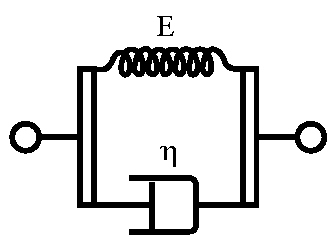
\includegraphics[width = 5 cm]{pics/Kelvin_Voigt_diagram.pdf}
  \caption{\textbf{Schematic overview of a Kelvin Voigt model.}}
  \label{fig:KelvinVoigt}
\end{figure}

The Young's modulus and initial radius of the vessel wall is divided into an active and a passive part and is a function of the attached myosin cross-bridges. The active and passive Young's modulus are based and fitted on experimental data of \citet{Gore} which is shown in Figure~\ref{fig:LinearisationRadius}. 

\begin{figure}[h!]
  \centering
  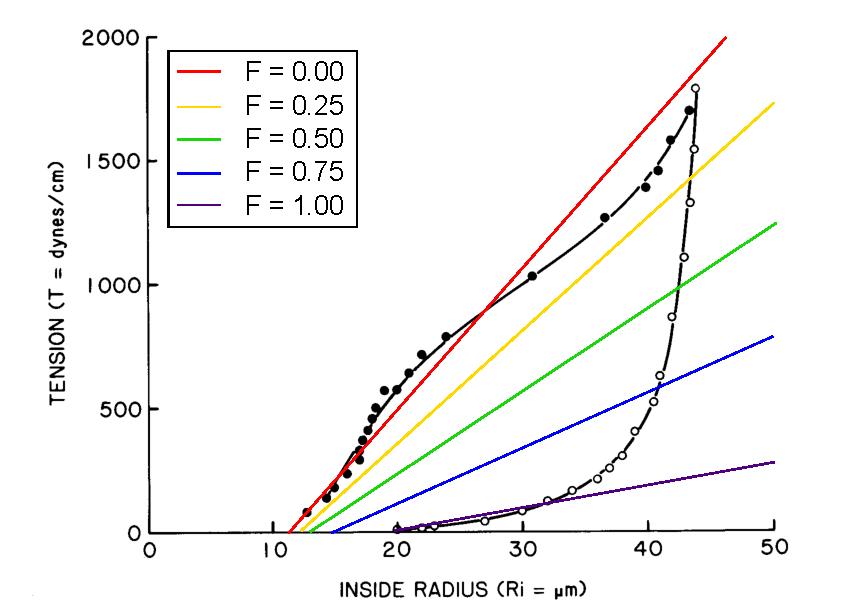
\includegraphics[width = 12 cm]{pics/LinearisationRadius.pdf}
  \caption{\textbf{Linearisation for the Young's modulus and initial radius on the data of \citet{Gore} for different values of F.}}
  \label{fig:LinearisationRadius}
\end{figure}

Figure~\ref{fig:LinearisationRadius} shows that the initial radius ($R_0$) decreases when the fraction of attached myosin cross bridges (F) are increased (the intersection with the x-axis). The figure also shows that the Young's modulus, represented by the slope of the lines in the tension-strain graph, increases when F increases. The linearisations of the Young's modulus can be described by:
\begin{equation} \label{eq:Fbalans4}
T=\frac{\Delta T}{\Delta R}(R-R_0)~,
\end{equation}
where $T$ is the tension of the vessel and $\frac{\Delta T}{\Delta R}$ is the slope of the linearisations in Figure~\ref{fig:LinearisationRadius}. \\

%Gore and Davis et al.\\
\newpage
\subsection{Merging of All Models}

The Astrocyte model and the \gls{SMC} and \gls{EC} model are linked by the SC and the \gls{PVS}. The \gls{K} input signal of the neuron is pumped into the \gls{SC} and taken up afterwards by the AC. The most important ion pumps and channels in this process are the \gls{K} channels in the neuron which releases the \gls{K} input,  the \gls{Na}/\gls{K} pump and \gls{K} channel in the \gls{AC} which pump the released \gls{K} into the AC.
The result of this is an efflux of \gls{K} at the end feet of the astrocyte using the BK-channel. Consequently, the membrane voltage of the astrocyte re-polarizes and the \gls{K} concentration in the PVS increases. This increased \gls{K} concentration activates the KIR channel in the \gls{SMC} and start to pump out more \gls{K} from the \gls{SMC} into the \gls{PVS}. The increased efflux of \gls{K} hyperpolarises the \gls{SMC} membrane voltage and as a result of that the VOCC closes and prevents the influx of \gls{Ca} into the \gls{SMC}.
Summarising, the neuronal input signal leads to a decrease of \gls{Ca} influx by the VOCC channels and therefore a decrease of the intracellular \gls{Ca} concentration. This leads to a decreased fraction of attached myosin bridges in the \citet{Hai1989} model, resulting in vessel dilation in the visco-elastic mechanical model. An overview of the whole model is shown in Figure~\ref{Overview}.

\begin{figure}[h!]
  \centering
  \def\svgwidth{450pt}
  \scriptsize 
  \import{pics/}{All_models_1pt1.pdf_tex}
  \caption{\textbf{All Models.}}
\label{Overview}
\end{figure}






%\begin{itemize}
%%\item What is the real relationship between the Ca concentration and the radius? - more references needed!
%%\item At the moment: Ca input of SMC, cross-bridge model of \citet{HaiMurphy}, Kelvin-Voigt model for elastic response of the arterial wall (assuming Laplace-law), change in radius 
%\end{itemize}


\section{Equations}

\subsection{Astrocyte Model}

\subsubsection{Scaling}
%
The  \gls{AC}  volume-area ratio (in $m$):
\begin{equation} \label{eq:R_k}
\dfrac{\mathrm{d}R_k}{\mathrm{d}t}= L_p \left( Na_k+K_k+Cl_k+HCO_{3_k}-Na_s-K_s-Cl_s-HCO_{3_{s}}+\frac{X_k}{R_k}\right)
\end{equation}
%
The \gls{SC} volume-surface ratio  (in $m$):
\begin{equation} \label{eq:R_tot}
R_s = R_{tot} - R_k  
\end{equation}
%
\begin{table}[h!]
\centering
\begin{tabular}{| p{0.09\linewidth} | >{\footnotesize} p{0.6\linewidth} | >{\footnotesize} p{0.17\linewidth} | >{\footnotesize} p{0.02\linewidth} |}
\arrayrulecolor{lightgrey}\hline
$L_p$ 			& The total water permeability per unit area of the astrocyte 			& 2.1e-9 \mperuMs &  \cite{Ostby2009}  \\
$X_k$			& Number of negatively charged impermeable ions trapped within the astrocyte divided by the astrocyte membrane area								& 12.41e-3 \uMm & \cite{Ostby2009}  \\
$R_{tot}$ 		& Total volume surface ratio AC+SC   		& 8.79e-8 \m & \cite{Ostby2009}  \\
\hline
\end{tabular}
\end{table}
\newpage
\subsubsection{Input Signal} \label{sec:InputSignal}
%
The neuronal \gls{K} input signal (-):\\
%
For $ t<t_0$ and $t>t_3$:
\begin{equation}
f(t)=0
\end{equation}
%
For $ t_0 \leq t \leq t_1$:
\begin{equation}
f(t)=F_{input} \dfrac{(\alpha+\beta-1)!}{(\alpha-1)!(\beta-1)!} \left( \dfrac{1-(t-t_0)}{\Delta t}\right) ^{\beta -1} \left( \dfrac{t-t_0}{\Delta t}\right) ^{\alpha -1} 
\end{equation}
%
For $ t_1 \leq t \leq t_2$:
\begin{equation}
f(t)=0
\end{equation}
%
For $ t_2 \leq t \leq t_3$:
\begin{equation}
f(t)=-F_{input}
\end{equation}
%
\begin{table}[h!]
\centering
\begin{tabular}{| p{0.09\linewidth} | >{\footnotesize} p{0.6\linewidth} | >{\footnotesize} p{0.17\linewidth} | >{\footnotesize} p{0.02\linewidth} |}
\arrayrulecolor{lightgrey}\hline
$t_0$ 			& Start of neuronal pulse	& 200 s &  ME  \\
$t_1$ 			& End of neuronal pulse	& 210 s &  ME  \\
$t_2$ 			& Start of back-buffering	& 230 s &  ME  \\
$t_3$ 			& End of back-buffering	& 240 s &  ME  \\
$F_{input}$ 	& Amplitude scaling factor 	& 2.5 	&  ME  \\
$\alpha$ 		& Beta-distribution constant	& 2 	&  ME  \\
$\beta$ 		& Beta-distribution constant	& 5 	&  ME  \\
$\Delta t$ 		& Time-scaling factor	& 10 s	&  ME  \\
\hline
\end{tabular}
\end{table}
% 
\subsubsection{Conservation Equations}
\paragraph{Synaptic Cleft}~\\
%
\gls{K} concentration in the \gls{SC} (times the \gls{SC} volume-area ratio $R_s$; in \uMm):
\begin{equation} \label{eq:KEx}
\dfrac{\mathrm{d}N_{K_s}}{\mathrm{d}t}= k_C f(t) -\dfrac{\mathrm{d}N_{K_k}}{\mathrm{d}t}
\end{equation}
%
\gls{Na} concentration in the \gls{SC}  (times the \gls{SC} volume-area ratio $R_s$; in \uMm):
\begin{equation} \label{eq:NaEx}
\dfrac{\mathrm{d}N_{Na_s}}{\mathrm{d}t}= - k_C f(t) -\dfrac{\mathrm{d}N_{Na_k}}{\mathrm{d}t}
\end{equation}
%
\gls{HCO3} concentration in the SC  (times the \gls{SC} volume-area ratio $R_s$; in \uMm):
\begin{equation} \label{eq:HCOEx}
\dfrac{\mathrm{d}N_{HCO_{3_{s}}}}{\mathrm{d}t}=-\dfrac{\mathrm{d}N_{HCO_{3_{k}}}}{\mathrm{d}t}
\end{equation}
\begin{table}[h!]
\centering
\begin{tabular}{| p{0.09\linewidth} | >{\footnotesize} p{0.6\linewidth} | >{\footnotesize} p{0.17\linewidth} | >{\footnotesize} p{0.02\linewidth} |}
\arrayrulecolor{lightgrey}\hline
$ k_C $  & Input scaling parameter & 7.35e-5 \muMps & \cite{Ostby2009} \\
\hline
\end{tabular}
\end{table}

\paragraph{Astrocyte}~\\
%
\gls{K} concentration in the AC  (times the AC volume-area ratio $R_k$; in \uMm):
\begin{equation} \label{eq:KInt}
\dfrac{\mathrm{d}N_{K_k}}{\mathrm{d}t}=- J_{K_k} + 2 J_{NaK_{k}} + J_{NKCC1_{k}} +  J_{KCC1_{k}}
- J_{BK_k}  
\end{equation}
%
\gls{Na} concentration in the AC  (times the AC volume-area ratio $R_k$; in \uMm):
\begin{equation} \label{eq:NaInt}
\dfrac{\mathrm{d}N_{Na_k}}{\mathrm{d}t}=-J_{Na_k} - 3 J_{NaK_{k}} + J_{NKCC1_{k}} +  J_{NBC_{k}}
\end{equation}
%
\gls{HCO3} concentration in the AC  (times the AC volume-area ratio $R_k$; in \uMm):
\begin{equation} \label{eq:HCOInt}
\dfrac{\mathrm{d}N_{HCO_{3_k}}}{\mathrm{d}t}= 2 J_{NBC_{k}} 
\end{equation}
%
\gls{Cl} concentration in the AC  (times the AC volume-area ratio $R_k$; in \uMm):
\begin{equation} \label{eq:ClInt}
\dfrac{\mathrm{d}N_{Cl_k}}{\mathrm{d}t}= \dfrac{\mathrm{d}N_{Na_k}}{\mathrm{d}t} + \dfrac{\mathrm{d}N_{K_k}}{\mathrm{d}t} - \dfrac{\mathrm{d}N_{HCO_{3_{k}}}}{\mathrm{d}t}
\end{equation}
%
Open probability of the BK channel (\pers):
\begin{equation} \label{eq:dwkdt}
\frac{\mathrm{d}w_{k}}{\mathrm{d}t} = \phi_{w} \left(w_{\infty}-w_{k} \right) 
\end{equation}
%
\paragraph{Perivascular Space}~\\
\gls{K} concentration in the PVS  (in \uM):
\begin{equation} \label{eq:K_p}
\dfrac{\mathrm{d}K_{p}}{\mathrm{d}t}= \frac{J_{BK_k}}{R_k VR_{pa}} + \frac{J_{KIR_i}}{ VR_{ps}}
\end{equation}
%
\begin{table}[h!]
\centering
\begin{tabular}{| p{0.09\linewidth} | >{\footnotesize} p{0.6\linewidth} | >{\footnotesize} p{0.17\linewidth} | >{\footnotesize} p{0.02\linewidth} |}
\arrayrulecolor{lightgrey}\hline
$ VR_{pa} $  & Volume ratio of PVS to AC & 0.001 [-] & \cite{LoesEvert} \\
$ VR_{ps} $  & Volume ratio of PVS to SMC & 0.001 [-] & \cite{LoesEvert} \\
\hline
\end{tabular}
\end{table}

\subsubsection{Fluxes}~\\
%
\gls{K} flux (times the AC volume-area ratio $R_k$; in \uMmps): 
\begin{equation} \label{eq:J_K}
J_{K_k}=\frac{g_{K_{k}}}{F}(v_k - E_{K_k}) C_{correction}
\end{equation}
%
\gls{Na} flux (times the AC volume-area ratio $R_k$; in \uMmps):
\begin{equation} \label{eq:J_Na}
J_{Na_k}=\frac{g_{Na_{k}}}{F}(v_k - E_{Na_k}) C_{correction}
\end{equation}
%
\gls{Na} and \gls{HCO3} flux through the NBC channel  (times the AC volume-area ratio $R_k$; in \uMmps): 
\begin{equation} \label{eq:J_NBC}
J_{NBC_k}=\frac{g_{NBC_k}}{F}\left(  v_k -E_{NBC_k}  \right) C_{correction}
\end{equation}
%
\gls{Cl} and \gls{K} flux through the KCC1 channel  (times the AC volume-area ratio $R_k$; in \uMmps): 
\begin{equation} \label{eq:J_KCC1}
J_{KCC1_k}=C_{input}\frac{g_{KCC1_k}}{F}\frac{RT}{F}ln \left(\frac{K_s Cl_s }{K_k Cl_k}\right) C_{correction}
\end{equation}
%
\gls{Na}, \gls{K} and \gls{Cl} flux through the NKCC1 channel   (times the AC volume-area ratio $R_k$; in \uMmps): 
\begin{equation} \label{eq:J_NKCC1}
J_{NKCC1_k}=C_{input}\frac{g_{NKCC1_k}}{F}\frac{RT}{F}ln \left(\frac{Na_s K_s {Cl_s}^2}{Na_k K_k {Cl_k}^2}\right) C_{correction}
\end{equation}
%
Flux through the sodium potassium pump   (times the \gls{AC} volume-area ratio $R_k$; in \uMmps): 
\begin{equation} \label{eq:J_NaK_s}
J_{NaK_{k}}=J_{NaK_{max}}\frac{{Na_k}^{1.5}}{{Na_k}^{1.5}+{K_{Na_k}}^{1.5}}\frac{K_s}{K_s+K_{K_s}}
\end{equation}
%
\gls{K} flux through the BK channel  (times the \gls{AC} volume-area ratio $R_k$; in \uMmps): 
\begin{equation} \label{eq:J_BK}
J_{BK_k}=\frac{g_{BK_k}}{F}w_k\left( v_k-E_{BK_k} \right) C_{correction}
\end{equation}
%
%
%
\begin{table}[h!]
\centering
\begin{tabular}{| p{0.09\linewidth} | >{\footnotesize} p{0.6\linewidth} | >{\footnotesize} p{0.17\linewidth} | >{\footnotesize} p{0.02\linewidth} |}
\arrayrulecolor{lightgrey}\hline	
$F$ 			& Faradays constant														& 9.649e4 \Cmol 	& \\
$R$ 			& Gas constant 															& 8.315 \JmolK		& \\
$T$ 	    	& Temperature 															& 300 \Kelvin		& \\
$g_{K_{k}}$ 	& Specific ion conductance of potassium 								& 40 \perOhmm 		& \cite{Ostby2009}  \\
$g_{Na_k}$ 		& Specific ion conductance of sodium 									& 1.314  \perOhmm 	& \cite{Ostby2009}  \\
$g_{NBC_k}$ 	& Specific ion conductance of the NBC cotransporter						& 7.57e-1 \perOhmm 	& \cite{Ostby2009}  \\
$g_{KCC1_k}$ 	& Specific ion conductance of the KCC1 cotransporter					& 1e-2 \perOhmm 	& \cite{Ostby2009}  \\
$g_{NKCC1_k}$ 	& Specific ion conductance of the NKCC1 cotransporter	 				& 5.54e-2 \perOhmm 	& \cite{Ostby2009}  \\
$J_{NaK_{max}}$ & The maximum flux through the NaKATPase pump							& 1.42e-3 \uMms 	& \cite{Ostby2009}  \\
$g_{BK_k}$ 		& Specific ion conductance of the BK channel							& 1.16     \perOhmm & \cite{LoesEvert}  \\
$C_{correction}$  & correction factor & 10$^3$ [-] & \cite{LoesEvert} \\
$C_{input}$  & Block function to switch the channel on and off &  0 ; 1 [-] & \cite{LoesEvert} \\
\hline
\end{tabular}
\end{table}



\newpage
\subsubsection{Additional Equations}
\paragraph{Synaptic Cleft}~\\
%
\gls{Cl} concentration  (times the SC volume-area ratio $R_s$; in \uMm): 
\begin{equation} \label{eq:ClEx}
N_{Cl_s}= N_{Na_s}+N_{K_s}-N_{ HCO_{3_s}}
\end{equation}

\paragraph{Astrocyte}~\\
%
Membrane voltage of the \gls{AC} (mV):
\begin{equation} \label{eq:v_k}
v_k=\frac{g_{Na_k}E_{Na_k}+g_{K_k}E_{K_k}+g_{Cl_k}E_{Cl_k}+g_{NBC_k}E_{NBC_k} + g_{BK_k}w_kE_{BK_k} -J_{NaK_k}F C_{correction} }{ g_{Na_k}+g_{K_k}+g_{Cl_k}+g_{NBC_k}+g_{BK_k}w_k }
\end{equation}
%
Nernst potential for the potassium channel (in mV):
\begin{equation} \label{eq:E_K}
E_{K_k}=\frac{RT}{z_K F}ln\left( \frac{K_s}{K_k}\right) 
\end{equation}
%
Nernst potential for the sodium channel (in mV):
\begin{equation} \label{eq:E_Na}
E_{Na_k}=\frac{RT}{z_{Na} F}ln\left( \frac{Na_s}{Na_k}\right) 
\end{equation}
%
Nernst potential for the chloride channel (in mV):
\begin{equation} \label{eq:E_Cl}
E_{Cl_k}=\frac{RT}{z_{Cl} F}ln\left( \frac{Cl_s}{Cl_k}\right) 
\end{equation}
%
Nernst potential for the NBC channel (in mV):
\begin{equation} \label{eq:E_NBC}
E_{NBC_k}=\frac{RT}{z_{NBC} F}ln\left( \frac{Na_s {HCO_{3_s}}^2}{Na_k {HCO_{3_k}}^2}\right) 
\end{equation}
Nernst potential for the BK channel (in mV):
\begin{equation} \label{eq:E_BK}
E_{BK_k}=\frac{RT}{z_K F}ln\left( \frac{K_p}{K_k}\right) 
\end{equation}
%
Equilibrium state BK-channel (-):
\begin{equation} \label{eq:winf}
w_{\infty}=0.5 \left(1+\mathrm{tanh}\left(\frac{v_{k}+v_{6} }{v_{4}} \right)  \right) 
\end{equation}
%
The time constant associated with the opening of BK channels	 (in \pers):
\begin{equation} \label{eq:phin}
\phi_{w}=\psi_{w}\mathrm{cosh}\left( \frac{v_{k}+v_{6}}{2v_{4}}\right) 
\end{equation}

\begin{table}[h!]
\centering
\begin{tabular}{| p{0.09\linewidth} | >{\footnotesize} p{0.6\linewidth} | >{\footnotesize} p{0.17\linewidth} | >{\footnotesize} p{0.02\linewidth} |}
\arrayrulecolor{lightgrey}\hline
$g_{Cl_k}$ 		& Specific ion conductance of chloride 									& 8.797e-1 \perOhmm & \cite{Ostby2009}  \\
$z_K$			& Valence of a potassium ion										& 1  [-] & \\ 
$z_Na$			& Valence of a sodium ion											& 1  [-] & \\ 
$z_Cl$			& Valence of a chloride ion											& -1 [-] & \\ 
$z_{NBC}$ 		& Effective valence of the NBC cotransporter complex 				& -1 [-] & \\
$v_{6}$			& The voltage associated with the opening of half the population		& 22e-3 \Volt  & \cite{LoesEvert}  \\
$v_{4}$			& A measure of the spread of the distribution of the open probability of the BK channel	& 14.5e-3 \Volt   &  \cite{Gonzalez1994}  
\\
$ \psi_{w}$    	& A characteristic time for the open probability of the BK channel		& 2.664 \pers & \cite{Gonzalez1994} \\

\hline
\end{tabular}
\end{table}




\newpage
\subsection{SMC and EC Model}


\subsubsection{Conservation Equations}
\paragraph{Smooth Muscle Cell}~\\
%
The cytosolic [\gls{Ca}] in the \gls{SMC} (in \uM):
\begin{equation}\label{eq:ci}
\begin{split}
\dfrac{\mathrm{d}\CaConsc}{\mathrm{d}t} = J_{IP_{3i}} - J_{SR_{uptake_{i}}} + J_{CICR_{i}} - J_{extrusion_{i}} +  J_{SR_{leak_{i}}}\dots \\
 - J_{VOCC_{i}} + J_{Na/Ca_{i}}  - 0.1J_{stretch_{i}} + J_{Ca^{2+}-coupling_{i}}^{SMC-EC}
\end{split} 
\end{equation}
%
The [Ca$^{2+}$] in the \gls{SR} of the \gls{SMC} (in \uM):
\begin{equation} \label{eq:si}
\dfrac{\mathrm{d}\CaConse}{\mathrm{d}t} =  J_{SR_{uptake_{i}}} - J_{CICR_{i}} - J_{SR_{leak_{i}}}
\end{equation}
%
The membrane potential of the \gls{SMC} (in \mV):
\begin{equation} \label{eq:vi}
\begin{split}
\dfrac{\mathrm{d}v_{i}}{\mathrm{d}t} = \gamma_{i}( -J_{Na/K_{i}} - J_{Cl_{i}} - 2J_{VOCC_{i}}- J_{Na/Ca_{i}} - J_{K_{i}} \dots \\
- J_{stretch_{i}} - J_{KIR_{i}} ) +V^{SMC-EC}_{coupling_{i}}
\end{split}
\end{equation}
%
The open state probability of calcium-activated potassium channels (dimensionless):
\begin{equation} \label{eq:dwidt}
\dfrac{\mathrm{d}w_{i}}{\mathrm{d}t} =  \lambda_{i} \left( K_{act_{i}} - w_{i} \right)
\end{equation}
%
The \gls{IP3} concentration om the \gls{SMC} (in \uM):
\begin{equation} \label{eq:dIidt}
\dfrac{\mathrm{d}\IP _{i}}{\mathrm{d}t} = J^{SMC-EC}_{IP_{3}-coupling_{i}} - J_{degrad_{i}}
\end{equation}
%
The \gls{K} concentration in the \gls{SMC} (in \uM):
\begin{equation} \label{eq:dkidt}
\dfrac{\mathrm{d} [K^+_{i}]}{\mathrm{d}t}  = J_{Na/K_{i}}  - J_{KIR_{i}} - J_{K_{i}}
\end{equation}

\begin{table}[h!]
\centering
\begin{tabular}{| p{0.09\linewidth} | >{\footnotesize} p{0.6\linewidth} | >{\footnotesize} p{0.17\linewidth} | >{\footnotesize} p{0.02\linewidth} |}
\arrayrulecolor{lightgrey}\hline
$\gamma_{i}$				& The change in membrane potential by a scaling factor					& 1970 \mVpuM	& \cite{Koenigsberger2006} \\
$\lambda_{i} $				& The rate constant for opening											& 45.0 \pers 	& \cite{Koenigsberger2006} \\
%$\CaConsc$      		& The cytololic [Ca$^{2+}$] in the SMC    								& var. \uM		& - \\
\hline
\end{tabular}
\label{tab:dcidt}
\end{table}

\paragraph{Endothelial Cell}~\\
%
The cytosolic \gls{Ca} concentration in the \gls{EC} (in \uM):
\begin{equation} \label{eq:cj}
\begin{split}
\dfrac{\mathrm{d}\CaConec}{\mathrm{d}t} = J_{IP_{3j}} - J_{ER_{uptake_{j}}} + J_{CICR_{j}} - J_{extrusion_{j}}\dots \\
 + J_{ER_{leak_{j}}} + J_{cation_{j}} + J_{0_{j}}- 0.1J_{stretch_{j}} - J_{Ca^{2+}-coupling_{j}}^{SMC-EC}
\end{split}
\end{equation}
%
The \gls{Ca} concentration in the \gls{ER} in the \gls{EC} (in \uM): %copied from SMC
\begin{equation} \label{eq:sj}
\dfrac{\mathrm{d}\CaConee}{\mathrm{d}t} =  J_{SR_{uptake_{j}}} - J_{CICR_{j}} - J_{SR_{leak_{j}}}
\end{equation}
%
The membrane potential of the \gls{EC} (in \mV):
\begin{equation} \label{eq:dvjdt}
\dfrac{\mathrm{d}v_{j}}{\mathrm{d}t} =-\frac{1}{C_{m_{j}}} ( J_{K_{j}}+J_{R_{j}}) + V^{SMC-EC}_{coupling_{j}}
\end{equation}
%
The \gls{IP3} concentration of the \gls{EC} (in \uM):
\begin{equation} \label{eq:dIjdt}
\dfrac{\mathrm{d}\IP_{j}}{\mathrm{d}t} =  J_{agonist_{j}}- J_{degrad_{j}}  - J^{SMC-EC}_{IP_{3}-coupling_{j}}
\end{equation}

\begin{table}[h!]
\centering
\begin{tabular}{| p{0.09\linewidth} | >{\footnotesize} p{0.6\linewidth} | >{\footnotesize} p{0.17\linewidth} | >{\footnotesize} p{0.02\linewidth} |}
\arrayrulecolor{lightgrey}\hline
 $C_{m_{j}}$				& Membrane capacitance												& 25.8  \pF		& \cite{Koenigsberger2006} \\
 
\hline
\end{tabular}
\label{tab:JSRuptakei}
\end{table}
%\\

\subsubsection{Fluxes}
%
\paragraph{Smooth Muscle Cell}~\\
%
The release of calcium from IP$_{3}$ sensitive stores in the SMC (in \uMps):
\begin{equation} \label{eq:IP3i}
J_{IP_{3i}} = F_{i}\frac{\IP_{i}^{2}}{K_{ri}^{2}+\IP_{i}^{2}}
\end{equation}
%
\begin{table}[h!]
\centering
\begin{tabular}{| p{0.09\linewidth} | >{\footnotesize} p{0.6\linewidth} | >{\footnotesize} p{0.17\linewidth} | >{\footnotesize} p{0.02\linewidth} |}
\arrayrulecolor{lightgrey}\hline
 $F_{i}$      			& Maximal rate of activation-dependent calcium influx			& 0.23 \uMps				& \cite{Koenigsberger2006} \\
$K_{ri}$				& Half-saturation constant for agonist-dependent calcium entry	& 1 \uM					& \cite{Koenigsberger2006} \\
\hline
\end{tabular}
\label{tab:IP3i}
\end{table}
\\
%
\newpage The uptake of calcium into the sarcoplasmic reticulum (in \uMs):
\begin{equation} \label{eq:JSRuptakei}
J_{SR_{uptake_{i}}} = B_{i}\frac{\CaConsc^{2}}{c_{bi}^{2}+\CaConsc^{2}}
\end{equation}
%
\begin{table}[h!]
\centering
\begin{tabular}{| p{0.09\linewidth} | >{\footnotesize} p{0.6\linewidth} | >{\footnotesize} p{0.17\linewidth} | >{\footnotesize} p{0.02\linewidth} |}
\arrayrulecolor{lightgrey}\hline
$B_{i}$      			& SR uptake rate constant							& 2.025 \uMs				& \cite{Koenigsberger2006} \\
$c_{bi}$				& Half-point of the SR ATPase activation sigmoidal (oder Michaelis (Menten) constant) 	& 1.0 \uM					& \cite{Koenigsberger2006} \\
\hline
\end{tabular}
\label{tab:JSRuptakei}
\end{table}
\\
%
The calcium-induced calcium release (CICR; in \uMs):
\begin{equation} \label{eq:JCICRi}
J_{CICR_{i}} = C_{i}\frac{\CaConse^{2}}{s_{ci}^{2}+\CaConse^{2}}    \frac{\CaConsc^{4}}{c_{ci}^{4}+\CaConsc^{4}}
\end{equation}
%
\begin{table}[h!]
\centering
\begin{tabular}{| p{0.09\linewidth} | >{\footnotesize} p{0.6\linewidth} | >{\footnotesize} p{0.17\linewidth} | >{\footnotesize} p{0.02\linewidth} |}
\arrayrulecolor{lightgrey}\hline
$C_{i}$      			& CICR rate constant									& 55 \uMs		& \cite{Koenigsberger2006} \\
$s_{ci}$				& Half-point of the CICR Ca$^{2+}$ efflux sigmoidal			& 2.0 \uM		& \cite{Koenigsberger2006} \\
$c_{ci}$				& Half-point of the CICR activation sigmoidal			& 0.9 \uM		& \cite{Koenigsberger2006} \\
\hline
\end{tabular}
\label{tab:JCICRi}
\end{table}
\\
%
The calcium extrusion by Ca$^{2+}$-ATPase pumps (in \uMs):
\begin{equation} \label{eq:Jextrusioni}
J_{extrusion_{i}} = D_{i}\CaConsc   \left( 1+ \frac{v_{i}-v_{d}}{R_{di}}\right)
\end{equation}
%
\begin{table}[h!]
\centering
\begin{tabular}{| p{0.09\linewidth} | >{\footnotesize} p{0.6\linewidth} | >{\footnotesize} p{0.17\linewidth} | >{\footnotesize} p{0.02\linewidth} |}
\arrayrulecolor{lightgrey}\hline
$D_{i}$      			& Rate constant for Ca$^{2+}$ extrusion by the ATPase pump		 & 0.24	\pers			& \cite{Koenigsberger2005} \\
$v_{d}$					& Intercept of voltage dependence of extrusion ATPase			 & -100.0 \mV			& \cite{Koenigsberger2006} \\
$R_{di}$				& Slope of voltage dependence of extrusion ATPase.				 & 250.0 \mV			& \cite{Koenigsberger2006} \\
\hline
\end{tabular}
\label{tab:Jextrusioni}
\end{table}
\\
%
The leak current from the SR (in \uMs):
\begin{equation} \label{eq:JSRleaki}
J_{SR_{leak_{i}}} = L_{i}\CaConse
\end{equation}
\begin{table}[h!]
\centering
\begin{tabular}{| p{0.09\linewidth} | >{\footnotesize} p{0.6\linewidth} | >{\footnotesize} p{0.17\linewidth} | >{\footnotesize} p{0.02\linewidth} |}
\arrayrulecolor{lightgrey}\hline
$L_{i}$      			& Leak from SR rate constant						 & 0.025 \pers				& \cite{Koenigsberger2006} \\
\hline
\end{tabular}
\label{tab:Jleaki}
\end{table}
\\
%
\newpage
The calcium influx through VOCCs (in \uMs): 
\begin{equation} \label{eq:JVOCCi}
J_{VOCC_{i}} = G_{Cai} \frac{v_{i}-v_{Ca_{1i}}}     {1+ exp(-\left[ \left(  v_{i}-v_{Ca_{2i}}\right) /R_{Cai}      \right] )}
\end{equation}
\begin{table}[h!]
\centering
\begin{tabular}{| p{0.09\linewidth} | >{\footnotesize} p{0.57\linewidth} | >{\footnotesize} p{0.2\linewidth} | >{\footnotesize} p{0.02\linewidth} |}
\arrayrulecolor{lightgrey}\hline
$G_{Cai}$      	& Whole-cell conductance for VOCCs	 					& 1.29e-3  \uMpmVs					& \cite{Koenigsberger2006} \\
$v_{Ca_{1i}}$   & Reversal potential for VOCCs	 						& 100.0 \mV							& \cite{Koenigsberger2006} \\
$v_{Ca_{2i}}$  	& Half-point of the VOCC activation sigmoidal		 	& -35.0 \mV							& ME \\
$R_{Cai}$      	& Maximum slope of the VOCC	activation sigmoidal		& 8.5 \mV							& \cite{Koenigsberger2006} \\
\hline
\end{tabular}
\label{tab:JVOCCi}
\end{table}
\\
%
The flux of calcium exchanging with sodium in the Na$^{+}$Ca$^{2+}$ exchange (in \uMs): 
\begin{equation} \label{eq:JNaCai}
J_{Na/Ca_{i}} = G_{Na/Ca_{i}} \frac{\CaConsc}     {\CaConsc + c_{Na/Cai}} \left( v_{i}-v_{Na/Ca_{i}} \right)
\end{equation}
%
\begin{table}[h!]
\centering
\begin{tabular}{| p{0.09\linewidth} | >{\footnotesize} p{0.57\linewidth} | >{\footnotesize} p{0.2\linewidth} | >{\footnotesize} p{0.02\linewidth} |}
\arrayrulecolor{lightgrey}\hline
$G_{Na/Cai}$   	& Whole-cell conductance for Na$^{+}$/Ca$^{2+}$ exchange			 		 & 3.16e-3 \uMpmVs	& \cite{Koenigsberger2005} \\
$c_{Na/Cai}$   	& Half-point for activation of Na$^{+}$/Ca$^{2+}$ exchange by Ca$^{2+}$		 & 0.5 \uM			& \cite{Koenigsberger2006} \\
$v_{Na/Cai}$   	& Reversal potential for the Na$^{+}$/Ca$^{2+}$ exchanger					 & -30.0 \mV		& \cite{Koenigsberger2006} \\
\hline
\end{tabular}
\label{tab:JNaCai}
\end{table}
\\
%
The calcium flux through the stretch-activated channels in the SMC (in \uMs): 
\begin{equation} \label{eq:Jstretchi}
\begin{split}
J_{stretch_{i}}= \frac{G_{stretch}}{1+ exp\left(-\alpha_{stretch}  \left(  \frac{\Delta pR}{h} -\sigma_{0}   \right) \right)}  \left(  v_{i}-E_{SAC}   \right) 
\end{split}
\end{equation}
%
\begin{table}[h!]
\centering
\begin{tabular}{| p{0.09\linewidth} | >{\footnotesize} p{0.57\linewidth} | >{\footnotesize} p{0.2\linewidth} | >{\footnotesize} p{0.02\linewidth} |}
\arrayrulecolor{lightgrey}\hline
$G_{stretch}$      		& The whole cell conductance for SACs						& 6.1e-3 \uMpmVs	&\cite{Koenigsberger2006} \\
$\alpha_{stretch}$      & Slope of stress dependence of the SAC activation sigmoidal	& 7.4e-3 \pmmHg	&\cite{Koenigsberger2006} \\
$ \Delta p $			& Pressure difference										& 30 \mmHg			& ME \\
$\sigma_{0}$      		& Half-point of the SAC activation sigmoidal				& 500 \mmHg			&\cite{Koenigsberger2006} \\
$E_{SAC}$      			& The reversal potential for SACs							& -18 \mV			&\cite{Koenigsberger2006} \\
\hline
\end{tabular}
\label{tab:Jstretchi}
\end{table}
\\
%
\newpage
Flux through the sodium potassium pump (in \uMs): 
\begin{equation} \label{eq:J_NaK_i}
J_{NaK_{i}}= F_{NaK}
\end{equation}
%
\begin{table}[h!]
\centering
\begin{tabular}{| p{0.09\linewidth} | >{\footnotesize} p{0.57\linewidth} | >{\footnotesize} p{0.2\linewidth} | >{\footnotesize} p{0.02\linewidth} |}
\arrayrulecolor{lightgrey}\hline
$F_{NaK}$      			& Rate of the potassium influx by the sodium potassium pump 		& 4.32e-2 \uMps 	&\cite{Koenigsberger2006} \\
\hline
\end{tabular}
\label{tab:JCli}
\end{table}
\\
Chloride flux through the chloride channel (in \uMs):
\begin{equation} \label{eq:JCli}
J_{Cl_{i}} = G_{Cli} \left(  v_{i} - v_{Cli}  \right) 
\end{equation}
%
\begin{table}[h!]
\centering
\begin{tabular}{| p{0.09\linewidth} | >{\footnotesize} p{0.57\linewidth} | >{\footnotesize} p{0.2\linewidth} | >{\footnotesize} p{0.02\linewidth} |}
\arrayrulecolor{lightgrey}\hline
$G_{Cli}$      			& Whole-cell conductance for Cl$^{-}$ current		& 1.34e-3 \uMpmVs	&\cite{Koenigsberger2006} \\
$v_{Cli}$      			& Reversal potential for Cl$^{-}$ channels.			& -25.0 \mV			&\cite{Koenigsberger2006} \\
\hline
\end{tabular}
\label{tab:JCli}
\end{table}
\\
%
Potassium flux through potassium channel (in \uMs):
\begin{equation} \label{eq:JKi}
J_{K_{i}}= G_{Ki} w_{i} \left(  v_{i} - vK_i  \right) 
\end{equation}
%
\begin{table}[h!]
\centering
\begin{tabular}{| p{0.09\linewidth} | >{\footnotesize} p{0.57\linewidth} | >{\footnotesize} p{0.2\linewidth} | >{\footnotesize} p{0.02\linewidth} |}
\arrayrulecolor{lightgrey}\hline
$G_{Ki}$      			& Whole-cell conductance for K$^{+}$ efflux.			& 4.46e-3 \uMpmVs	&\cite{Koenigsberger2005} \\
$vK_i$      			& Nernst potential										& -94 \mV	&\cite{Koenigsberger2005} \\
\hline
\end{tabular}
\label{tab:JKi}
\end{table}
\\
The flux through KIR channels in the SMC (in \uMs): 
\begin{equation} \label{eq:JKIRi}
J_{KIR_{i}} =  \frac{F_{KIR_{i}} g_{KIR_{i}}}{\gamma_{i}}( v_{i} - v_{KIR_{i}})
\end{equation}
%
\begin{table}[h!]
\centering
\begin{tabular}{| p{0.09\linewidth} | >{\footnotesize} p{0.57\linewidth} | >{\footnotesize} p{0.2\linewidth} | >{\footnotesize} p{0.02\linewidth} |}
\arrayrulecolor{lightgrey}\hline
$ F_{KIR_{i}} $ & Scaling factor of potassium efflux through the KIR channel & 7.5e2 & \cite{LoesEvert} \\
\hline
\end{tabular}
\label{tab:JCli}
\end{table}
\\
The IP$_{3}$ degradation (in \uMs): 
\begin{equation} \label{eq:Jdegradi}
J_{degrad_{i}}= k_{di}I_{i}
\end{equation}
\begin{table}[h!]
\centering
\begin{tabular}{| p{0.09\linewidth} | >{\footnotesize} p{0.57\linewidth} | >{\footnotesize} p{0.2\linewidth} | >{\footnotesize} p{0.02\linewidth} |}
\arrayrulecolor{lightgrey}\hline
$k_{di}$      			& Rate constant of IP$_{3}$ degradation	& 0.1 \pers	&\cite{Koenigsberger2006} \\
\hline
\end{tabular}
\label{tab:Jdegradi}
\end{table}
%
\newpage
\paragraph{Endothelial Cell}~\\
\\
%
The release of calcium from IP$_{3}$-sensitive stores in the EC (in \uMps):
\begin{equation} \label{eq:JIP3j}
J_{IP_{3j}} = F_{j}\frac{\IP_{j}^{2}}{K_{rj}^{2}+\IP_{j}^{2}}
\end{equation}
\begin{table}[h!]
\centering
\begin{tabular}{| p{0.09\linewidth} | >{\footnotesize} p{0.6\linewidth} | >{\footnotesize} p{0.17\linewidth} | >{\footnotesize} p{0.02\linewidth} |}
\arrayrulecolor{lightgrey}\hline
 $F_{j}$      			& Maximal rate of activation-dependent calcium influx			& 0.23 \uMps				& \cite{Koenigsberger2006} \\
$K_{rj}$				& Half-saturation constant for agonist-dependent calcium entry	& 1 \uM					& \cite{Koenigsberger2006} \\
\hline
\end{tabular}
\label{tab:IP3j}
\end{table}
\\
%
The uptake of calcium into the endoplasmic reticulum (in \uMs):
\begin{equation} \label{eq:JERuptakej}
J_{ER_{uptake_{j}}} = B_{j}\frac{\CaConec^{2}}{c_{bj}^{2}+\CaConec^{2}}
\end{equation}
%
\begin{table}[h!]
\centering
\begin{tabular}{| p{0.09\linewidth} | >{\footnotesize} p{0.6\linewidth} | >{\footnotesize} p{0.17\linewidth} | >{\footnotesize} p{0.02\linewidth} |}
\arrayrulecolor{lightgrey}\hline
$B_{j}$      			& ER uptake rate constant							& 0.5 \uMs				& \cite{Koenigsberger2006} \\
$c_{bj}$				& Half-point of the SR ATPase activation sigmoidal (oder Michaelis (Menten) constant) 	& 1.0 \uM					& \cite{Koenigsberger2006} \\
\hline
\end{tabular}
\label{tab:JERuptakej}
\end{table}
\\
%
The calcium-induced calcium release (CICR; in \uMs):
\begin{equation} \label{eq:JCICRJ}
J_{CICR_{j}} = C_{j}\frac{\CaConee^{2}}{s_{cj}^{2}+\CaConee^{2}}    \frac{\CaConec^{4}}{c_{cj}^{4}+\CaConec^{4}}
\end{equation}
%
\begin{table}[h!]
\centering
\begin{tabular}{| p{0.09\linewidth} | >{\footnotesize} p{0.6\linewidth} | >{\footnotesize} p{0.17\linewidth} | >{\footnotesize} p{0.02\linewidth} |}
\arrayrulecolor{lightgrey}\hline
$C_{j}$      			& CICR rate constant									& 5 \uMs		& \cite{Koenigsberger2006} \\
$s_{cj}$				& Half-point of the CICR Ca$^{2+}$ efflux sigmoidal			& 2.0 \uM		& \cite{Koenigsberger2006} \\
$c_{cj}$				& Half-point of the CICR activation sigmoidal			& 0.9 \uM		& \cite{Koenigsberger2006} \\
\hline
\end{tabular}
\label{tab:JCICRj}
\end{table}
\\
The calcium extrusion by Ca$^{2+}$-ATPase pumps (in \uMs):
\begin{equation} \label{eq:Jextrusionj}
J_{extrusion_{j}} = D_{j}\CaConec 
\end{equation}
%
%
\begin{table}[h!]
\centering
\begin{tabular}{| p{0.09\linewidth} | >{\footnotesize} p{0.6\linewidth} | >{\footnotesize} p{0.17\linewidth} | >{\footnotesize} p{0.02\linewidth} |}
\arrayrulecolor{lightgrey}\hline
$D_{j}$      			& Rate constant for Ca$^{2+}$ extrusion by the ATPase pump		 & 0.24	\pers			& \cite{Koenigsberger2005} \\
\hline
\end{tabular}
\label{tab:Jextrusionj}
\end{table}
\\
%
\newpage 
The calcium flux through the stretch-activated channels in the EC (in \uMs): 
\begin{equation} \label{eq:Jstretchj}
J_{stretch_{j}}= \frac{G_{stretch}}{1+ e^{-\alpha_{stretch}  \left(  \sigma -\sigma_{0}   \right) }}  \left(  v_{j}-E_{SAC}   \right) \\
= \frac{G_{stretch}}{1+ e^{-\alpha_{stretch}  \left(  \frac{\Delta pR}{h} -\sigma_{0}   \right) }}  \left(  v_{j}-E_{SAC}   \right) 
\end{equation}
%
\begin{table}[h!]
\centering
\begin{tabular}{| p{0.09\linewidth} | >{\footnotesize} p{0.6\linewidth} | >{\footnotesize} p{0.17\linewidth} | >{\footnotesize} p{0.02\linewidth} |}
\arrayrulecolor{lightgrey}\hline
$G_{stretch}$      		& The whole cell conductance for SACs						& 6.1e-3 \uMpmVs	&\cite{Koenigsberger2006} \\
$\alpha_{stretch}$      & Slope of stress dependence of the SAC activation sigmoidal	& 7.4e-3 \pmmHg	&\cite{Koenigsberger2006} \\
$ \Delta p $			& Pressure difference										& 30 \mmHg			& ME \\
$\sigma_{0}$      		& Half-point of the SAC activation sigmoidal				& 500 \mmHg			&\cite{Koenigsberger2006} \\
$E_{SAC}$      			& The reversal potential for SACs							& -18 \mV			&\cite{Koenigsberger2006} \\
\hline
\end{tabular}
\label{tab:Jstretchj}
\end{table}
\\
%
The leak current from the ER (in \uMs):
\begin{equation} \label{eq:JERleakj}
J_{ER_{leak_{j}}} = L_{j}\CaConee
\end{equation}
%
\begin{table}[h!]
\centering
\begin{tabular}{| p{0.09\linewidth} | >{\footnotesize} p{0.6\linewidth} | >{\footnotesize} p{0.17\linewidth} | >{\footnotesize} p{0.02\linewidth} |}
\arrayrulecolor{lightgrey}\hline
$L_{j}$      			& Rate constant for Ca$^{2+}$ leak from the ER 		 & 0.025	\pers			& \cite{Koenigsberger2006} \\
\hline
\end{tabular}
\label{tab:JKj}
\end{table}
\\
%
The calcium influx through nonselective cation channels (in \uMs):
\begin{equation} \label{eq:Jcationj}
J_{cation_{j}} = G_{cat_{j}} (E_{Ca_{j}} - v_{j}) \frac{1}{2} \left(   1+ \mathrm{tanh}  \left(  \frac{\mathrm{log}_{10} \CaConec - m_{3_{cat_{j}}} }    {m_{4_{cat_{j}}}}   \right)      \right) 
\end{equation}
%
%
\begin{table}[h!]
\centering
\begin{tabular}{| p{0.09\linewidth} | >{\footnotesize} p{0.6\linewidth} | >{\footnotesize} p{0.17\linewidth} | >{\footnotesize} p{0.02\linewidth} |}
\arrayrulecolor{lightgrey}\hline
$G_{cat j}$      		& Whole-cell cation channel conductivity						 	& 6.6e-4 \uMpmVs	& \cite{Koenigsberger2006} \\
$E_{Caj}$      			& Ca$^{2+}$ equilibrium potential								 	& 50 \mV		& \cite{Koenigsberger2006} \\

$m_{3_{catj}}$      	& Model constant				 	& -6.18 \uM		& \cite{Koenigsberger2006} \\
$m_{4_{catj}}$      	& Model constant					& 0.37  \uM		& \cite{Koenigsberger2006} \\
\hline
\end{tabular}
\label{tab:Jcationj}
\end{table}
\\
%
The potassium efflux through the $J_{BK_{Caj}}$ channel and the $J_{SK_{Caj}}$ channel (in \uMs):
\begin{equation} \label{eq:JKj}
J_{K_{j}} = G_{totj} (v_{j}-v_{Kj}) \left(   J_{BK_{Caj}} + J_{SK_{Caj}} \right) 
\end{equation}
%
%
\begin{table}[h!]
\centering
\begin{tabular}{| p{0.09\linewidth} | >{\footnotesize} p{0.6\linewidth} | >{\footnotesize} p{0.17\linewidth} | >{\footnotesize} p{0.02\linewidth} |}
\arrayrulecolor{lightgrey}\hline
$G_{totj}$      		& Total potassium channel conductivity.						 		& 6927 \pS		& \cite{Koenigsberger2006} \\
$v_{Kj}$      			& K$^{+}$ equilibrium potential					 			 		& -80.0 \mV		& \cite{Koenigsberger2006} \\
\hline
\end{tabular}
\label{tab:JKj}
\end{table}
\\
%
The potassium efflux through the $J_{BK_{Caj}}$ channel (in \uMs):
\begin{equation} \label{eq:JBKCAj}
J_{BK_{Caj}} = 0.2 \left(   1+ \mathrm{tanh}   \left(   \frac{   (\mathrm{log}_{10} \CaConec - c) (v_{j}-b_{j}) - a_{1j}  }   { m_{3bj} ( v_{j} + a_{2j} (\mathrm{log}_{10} \CaConec -c )-b_{j} )^{2} + m_{4bj} }  \right)     \right)  
\end{equation}
%
The potassium efflux through the $J_{SK_{Caj}}$ channel (in \uMs):
\begin{equation} \label{eq:JSKCaj}
J_{SK_{Caj}} = 0.3\left( 1+ \mathrm{tanh}  \left(  \frac{   \mathrm{log}_{10} \CaConec -m_{3sj}  } {m_{4sj}}  \right)      \right) 
\end{equation}
%
\begin{table}[h!]
\centering
\begin{tabular}{| p{0.09\linewidth} | >{\footnotesize} p{0.6\linewidth} | >{\footnotesize} p{0.17\linewidth} | >{\footnotesize} p{0.02\linewidth} |}
\arrayrulecolor{lightgrey}\hline
$c$      				& Model constant, further explanation see reference					& -6.4 \uM			& \cite{Koenigsberger2006} \\
$b_{j}$      			& Model constant, further explanation see reference					& -80.8 \mV		& \cite{Koenigsberger2006} \\
$a_{1j}$      			& Model constant, further explanation see reference					& 53.3 \uMkeermV	& \cite{Koenigsberger2006} \\
$a_{2j}$      			& Model constant, further explanation see reference					& 53.3 \mVpuM		& \cite{Koenigsberger2006} \\
$m_{3bj}$      			& Model constant, further explanation see reference					& 1.32e-3 \uMpmV	& \cite{Koenigsberger2006} \\
$m_{4bj}$      			& Model constant, further explanation see reference					& 0.30	\uMkeermV	& \cite{Koenigsberger2006} \\
$m_{3sj}$      			& Model constant, further explanation see reference					& -0.28 \uM		& \cite{Koenigsberger2006} \\
$m_{4sj}$      			& Model constant, further explanation see reference					& 0.389 \uM		& \cite{Koenigsberger2006} \\
\hline
\end{tabular}
\label{tab:JBKCAj}
\end{table}
\\
%
The residual current regrouping chloride and sodium current flux (in \uMs):
\begin{equation} \label{eq:JRj}
J_{R_{j}} = G_{R_{j}} ( v_{j} - v_{rest j}  )
\end{equation}
%
\begin{table}[h!]
\centering
\begin{tabular}{| p{0.09\linewidth} | >{\footnotesize} p{0.6\linewidth} | >{\footnotesize} p{0.17\linewidth} | >{\footnotesize} p{0.02\linewidth} |}
\arrayrulecolor{lightgrey}\hline
$G_{R_{j}}$      		& Residual current conductivity										& 955 \pS			& \cite{Koenigsberger2006} \\
$v_{rest j}$      		& Membrane resting potential						 				& -31.1 \mV		& \cite{Koenigsberger2006} \\
\hline
\end{tabular}
\label{tab:JRj}
\end{table}
\\
%
The IP$_{3}$ degradation (in \uMs):  
\begin{equation} \label{eq:Jdegradj}
J_{degrad_{j}}= k_{dj} \IP_{j}
\end{equation}
%
\begin{table}[h!]
\centering
\begin{tabular}{| p{0.09\linewidth} | >{\footnotesize} p{0.6\linewidth} | >{\footnotesize} p{0.17\linewidth} | >{\footnotesize} p{0.02\linewidth} |}
\arrayrulecolor{lightgrey}\hline
$k_{dj}$      			& Rate constant of IP$_{3}$ degradation						 		& 0.1 \pers		& \cite{Koenigsberger2006} \\
\hline
\end{tabular}
\label{tab:Jdegradj}
\end{table}
\\
%
%
\subsubsection{Coupling}~\\
%
The heterocellular electrical coupling between SMCs en ECs (in \mVs):
\begin{equation} \label{eq:Vcouplingi}
V_{coupling_{i}}^{SMC-EC}= -G_{coup}(v_{i}-v_{j})
\end{equation}
%
The heterocellular IP$_{3}$ coupling between SMCs and ECs (in \uMs):
\begin{equation} \label{eq:JIP3couplingi}
J_{IP_{3}-coupling_{i}}^{SMC-EC}= -P_{IP_{3}}(\IP_{i}-\IP_{j})
\end{equation}
%
Calcium coupling with EC (in\uMs):
\begin{equation} \label{eq:JCAcouplingi}
J_{Ca^{2+}-coupling_{i}}^{SMC-EC}= -P_{Ca^{2+}}(\CaConsc-\CaConec)
\end{equation}
%
\begin{table}[h!]
\centering
\begin{tabular}{| p{0.09\linewidth} | >{\footnotesize} p{0.6\linewidth} | >{\footnotesize} p{0.17\linewidth} | >{\footnotesize} p{0.02\linewidth} |}
\arrayrulecolor{lightgrey}\hline
$P_{CA^{2+}}$      		& Heterocellular $P_{Ca^{2+}}$ coupling coefficient	& 0.05 \pers	&  \cite{Koenigsberger2006} \\
$P_{IP_{3}}$      		& Heterocellular IP$_{3}$ coupling coefficient	& 0.05 \pers	&  \cite{Koenigsberger2006} \\
$G_{coup}$      		& Heterocellular electrical coupling coefficient		& 5 \pers	& ME \\
\hline
\end{tabular}
\label{tab:JCA3couplingi}
\end{table}
%
\newpage
\subsubsection{Additional Equations}
%
The equilibrium distribution of open channel states for the voltage and calcium activated potassium channels (dimensionless):
\begin{equation} \label{eq:Kacti}
K_{act_{i}}= \frac{  \left( \CaConsc + c_{wi}\right)^{2}}    {\left( \CaConsc + c_{wi} \right)^{2}    + \beta_{i} exp( -\left(   \left[ v_{i}-v_{Ca_{3i}}\right] /R_{Ki}   \right) )      }
\end{equation}
%
Nernst potential of the KIR channel in the SMC (in mV):
\begin{equation}\label{eq:vKIR}
v_{KIR_i} = z_1 K_p-z_2
\end{equation}
%
Conductance of KIR channel (in  s$^{-1} $):
\begin{equation}\label{eq:gKIR}
g_{KIR_i} = exp(z_5v_i +z_3 K_p - z_4)
\end{equation}
%
%
%
\begin{table}[h!]
\centering
\begin{tabular}{| p{0.09\linewidth} | >{\footnotesize} p{0.6\linewidth} | >{\footnotesize} p{0.17\linewidth} | >{\footnotesize} p{0.02\linewidth} |}
\arrayrulecolor{lightgrey}\hline
$c_{wi}$      			& Translation factor for Ca$^{2+}$ dependence of K$_{Ca}$ channel activation sigmoidal.	& 0.0  \uM	&\cite{Koenigsberger2006} \\
$\beta_{i}$     		& Translation factor for membrane potential dependence of K$_{Ca}$ channel activation sigmoidal.	& 0.13 \uMtwee& \cite{Koenigsberger2006} \\
$v_{Ca_{3i}}$   		& Half-point for the K$_{Ca}$ channel activation sigmoidal.			& -27 \mV	&\cite{Koenigsberger2006} \\
$R_{Ki}$      			& Maximum slope of the K$_{Ca}$ activation sigmoidal.				& 12 \mV	&\cite{Koenigsberger2006} \\
$z_{1}$      			& Model estimation for membrane voltage KIR channel				& 4.5e3 \mV	&\cite{LoesEvert}  \\
$z_{2}$      			& Model estimation for membrane voltage KIR channel			& 112 \mV	&\cite{LoesEvert}  \\
$z_{3}$      			& Model estimation for the KIR channel conductance				& 4.2e2 \uMpmVs	&\cite{LoesEvert}  \\
$z_{4}$      			& Model estimation for the KIR channel conductance				& 12.6 \uMpmVs	&\cite{LoesEvert}  \\
$z_{5}$      			& Model estimation for the KIR channel conductance			& -7.4e-2 \uMpmVs	&\cite{LoesEvert}  \\
\hline
\end{tabular}
\label{tab:Addeq}
\end{table}
\\
%
\newpage
\subsection{Contraction and Mechanical Model}

\subsubsection{Contraction Equations}
%
The fraction of free phosphorylated cross-bridges (dimensionless):
\begin{equation} \label{eq:dMpdt}
\frac{\dd[Mp]}{\dd t} = K_{4_{i}}[AMp] +K_{1_{i}} [M] - ( K_{2_{i}} + K_{3_{i}} ) [Mp]
\end{equation}
%
The fraction of attached phosphorylated cross-bridges (dimensionless):
\begin{equation} \label{eq:dAMpdt}
\frac{\dd[AMp]}{\dd t} =K_{3_{i}} [Mp] + K_{6_{i}} [AM] - ( K_{4_{i}} + K_{5_{i}} )[AMp]
\end{equation} 
%
The fraction of attached dephosphorylated cross-bridges (dimensionless):
\begin{equation} \label{eq:dAMdt}
\frac{\dd[AM]}{\dd t} = K_{5_{i}} [AMp]-(K_{7_{i}}+K_{6_{i}})[AM]
\end{equation}
%
The fraction of free non-phosphorylated cross-bridges (dimensionless):
\begin{equation} \label{eq:dMdt}
[M]=1-[AM]-[AMp]-[Mp]
%\frac{\dd[M]}{\dd t} = -K_{1_{i}} [M] + K_{2_{i}} [Mp] + K_{7_{i}} [AM]
\end{equation}
%
The rate constants that represent phosphorylation of M to Mp and of AM to AMp by the active myosin light chain kinase (MLCK), respectively (in \pers):
\begin{equation} \label{eq:gamma}
K_{1_{i}} = K_{6_{i}} = \gamma_{cross} \CaConsc ^{3}
\end{equation}
%
%Note that:
%\begin{equation} \label{eq:fractiesone}
%[AM]+[AMp]+[Mp]+[M]=1
%\end{equation}
%
\begin{table}[h!]
\centering
\begin{tabular}{| p{0.09\linewidth} | >{\footnotesize} p{0.6\linewidth} | >{\footnotesize} p{0.17\linewidth} | >{\footnotesize} p{0.02\linewidth} |}
\arrayrulecolor{lightgrey}\hline
$K_{2_{i}}$      	& The rate constant for dephosphorylation (of Mp to M) by myosin light-chain phosphatase (MLCP)																			 & 0.5 \pers & \cite{Hai1989} \\
$K_{3_{i}}$      	& The rate constants representing the attachment/detachment of fast cycling phosphorylated crossbridges																	 & 0.4 \pers	& \cite{Hai1989} \\
$K_{4_{i}}$      	& The rate constants representing the attachment/detachment of fast cycling phosphorylated crossbridges 																	 & 0.1 \pers	& \cite{Hai1989} \\
$K_{5_{i}}$      & The rate constant for dephosphorylation (of AMp to AM) by myosin light-chain phosphatase (MLCP)																			 & 0.5 \pers	& \cite{Hai1989} \\
$K_{7_{i}}$      	& The rate constant for latch-bridge detachment					& 0.1 \pers	& \cite{Hai1989} \\
$\gamma_{cross}$      	& The sensitivity of the contractile apparatus to calcium		& 17 \puMdries	& \cite{Hai1989} \\
%$n_{cross}$      		& A constant for further explanation see reference				& 3 \Dless	& \cite{Hai1988} \\
\hline
\end{tabular}
%\caption{This table shows some data}
\label{tab:crossbridge}
\end{table}
\newpage
\subsubsection{Mechanical Equations}

The wall thickness of the vessel (in \um):
\begin{equation} \label{eq:h2}
h=-R+\sqrt{R^2+2R_{0_{pas}}h_{0_{pas}}+h_{0_{pas}}^2}
\end{equation}
%
The fraction of attached myosin cross-bridges (dimensionless):
\begin{equation}
F_r = [AM_p] + [AM]
\end{equation}
%
The vessel radius (in \um):
\begin{equation} \label{eq:dRdt2}
\dfrac{\mathrm{d}R}{\mathrm{d}t}= \frac{R_{0_{pas}}}{\eta}\left(   \frac{ R P_{T}}{h}  - E(F_r) \frac{R - R_0(F_r)}{R_0(F_r)} \right)
\end{equation}
%
with:
\begin{equation}
E(F_r)= E_{pas} + F_r \left(E_{act} - E_{pas} \right)
\end{equation}
%
\begin{equation}
R_0(F_r)=R_{0_{pas}} + F_r (\alpha -1) R_{0_{pas}}
\end{equation}
%
\begin{table}[h!]
\centering
\begin{tabular}{| p{0.09\linewidth} | >{\footnotesize} p{0.6\linewidth} | >{\footnotesize} p{0.17\linewidth} | >{\footnotesize} p{0.02\linewidth} |}
\arrayrulecolor{lightgrey}\hline
$\eta   $				& viscosity															& 1e4 Pa m 		&  \cite{Koenigsberger2006}\\
$R_{0_{pas}}$			& Radius of the vessel when passive and no stress is applied		& 20  \um 		& ME \\
$h_{0_{pas}}$			& Wall thickness when passive and no stress is applied				& 3   \um		& ME \\
$P_T$					& Transmural pressure												& 4000 \Pa		& ME \\
${E}_{pas}$				& Young's moduli for the passive vessel								& 66e3 \Pa 		&  \cite{Gore}\\
${E}_{act}$				& Additional component of the Young's moduli when vessel is active	& 167e3 \Pa 	& \cite{Gore}\\
$\alpha$				& Scaling factor initial radius										& 0.6    		& \cite{Gore}\\
\hline
\end{tabular}
%\caption{This table shows some data}
\label{tab:crossbridge}
\end{table}



\section{Code Structure}
%\todo{check all filenames! Loes and Evert used different ones than I did!}

The main script of the code is named \textit{'NVC\_main.m'} and calls all the needed functions and other scripts. A graphic structure diagram is given in Figure~\ref{fig:Structure}.\\
\textit{'all\_constants.m'} contains all variables used in the model and is created to give a clear overview and  furthermore to make it easy to recognize if variables are defined twice in the code inadvertently. In \textit{'all\_indices.m'} indices are defined for all differential equations (stored in the structure \textit{ind}) and all fluxes (stored in the structure \textit{flu}). 

The fluxes and other non-differential equations are stored in \textit{'all\_fluxes.m'}. Here, a separate array is defined for each cell (NE, AC, SMC, EC) to create a clearly arranged structure. The indices refer to the corresponding cell type or domain (NE - n, AC - k, SMC - i, EC - j).\\
The mass conservation equations describing the time-dependent rate of change for each species concentration and membrane voltage, respectively, are stored in \textit{'DEsyst.m'}. In the main script an ODE solver with adjustable options is chosen to solve the set of ordinary differential equations. The  solution for each iteration step and the corresponding time are stored in the two variables \textit{state} and \textit{time}, respectively.  The functions \textit{'odeprog()'} and \textit{'odeabort()'}  \cite{Franklin} give a GUI  with a visual progress bar to show the approximate remaining time and allow to abort the equation solving process via the \textit{'Abort'}-button. After each iteration step the function \textit{'writeFlux()'} is called to write each flux and ode solution, the corresponding flowrate (right hand side of the ODE) and time step into the array structure $DATA $. The stored values are used by the function \textit{ 'plot\_all.m'} to plot different state variables or fluxes. \\
The values of the two global variables $ CASE $ and $ J\_PLC $ can be changed in the main script in order to obtain different coupling strengths and binding agonist concentration, respectively. Also the value of NVU can be varied to execute either the NVU 1.0 of the NVU 1.1 model or look at the separate effects of Calcium and EET on the BK-channel open state.

\begin{figure}[h!]
  \centering
  \def\svgwidth{450pt} %400pt
  \footnotesize
  \import{pics/}{structure_diagram2.pdf_tex}
  \caption{\textbf{Diagram to illustrate the code structure.} The main script (\textit{'NVC\_main.m'}) calls an ode solver which solves the set of differential equations iteratively and stores the solution of each time step into a data file.}
\label{fig:Structure}
\end{figure}


%include contain defines 

%\todo[inline]{What is the expected PLC agonist concentration in the EC?}
%test
\section{Results}

\subsection*{Potassium input signal (figure \ref{fig:K})}
At the top the neuronal \gls{K} input signal is shown. This input signal is pumped into the SC by the \gls{NE}. As a result of that, there is more \gls{K} taken up by the \gls{AC} in the beginning of the input pulse, and released at the end of the input pulse. In the second graph the membrane potential of the AC is shown over time. When the \gls{K} concentration in the SC is increased the membrane voltage depolarizes and when the \gls{K} concentration in the SC decreases the membrane potential repolarizes again.
In the third graph the fluxes into the PVS are shown. In blue the flux by the astrocytic BK channel, and in green the flux by the KIR channel in the SMC is shown. The drop in the middle of the KIR flux is caused because the SMC becomes in a oscillation state and therefore the efflux by the KIR channel follows the \gls{Ca} waves inside the SMC.
The bottom figure shows the \gls{K} concentration in the PVS.

\subsection*{SMC and EC fluxes (figure \ref{fig:SMCfluxes} and \ref{fig:ECfluxes})}
In these figures the coupling and the fluxes in the SMC and EC are shown. When one of the fluxes is negative, it means that the direction of the flux is in the opposite than it is defined in the equations. These figures show also that when the neuronal signal is given, the VOCC closes and that the SMC goes into an oscillation state. 

\subsection*{Conservation equations (figure \ref{fig:dfdt})}
The graphs in this figure shows the solutions of the differential equations of the \gls{SMC} and \gls{EC}. The graphs on the left side are the SMC results, and at the right side the EC results. From top to bottom the following parameters are shown over time: the intracellular \gls{Ca} concentration, the \gls{IP3} concentration, the sarcoplasmic (\gls{SMC}) or endoplasmic (\gls{EC}) \gls{Ca} concentration, the membrane voltage and at the bottom for the SMC the open probability of the \gls{K} channels.

\subsection*{Hai and Murphy and radius model (figure \ref{fig:Radius})}
In this figure the fraction of the four states (M, Mp, AMp, AM) of myosin in the \cite{Hai1989} are shown at the top. At the bottom left the fraction of attached cross bridged myosin (the sum of AM and AMp) is shown. And at the bottom right the radius is plotted over time. The increase in vessel diameter is in the expected order of magnitude, however the slope is less steep than expected.

\begin{landscape} 
\begin{figure}[h!]
	\centering
	\tiny 
	\setlength\figureheight{2.5 cm} 
	\setlength\figurewidth{18 cm}
	% This file was created by matlab2tikz v0.3.3.
% Copyright (c) 2008--2013, Nico Schlömer <nico.schloemer@gmail.com>
% All rights reserved.
% 
% The latest updates can be retrieved from
%   http://www.mathworks.com/matlabcentral/fileexchange/22022-matlab2tikz
% where you can also make suggestions and rate matlab2tikz.
% 
% 
% 
\begin{tikzpicture}

\begin{axis}[%
width=\figurewidth,
height=\figureheight,
scale only axis,
xmin=0,
xmax=300,
xlabel={Time [s]},
separate axis lines,
every outer y axis line/.append style={blue},
every y tick label/.append style={font=\color{blue}},
ymin=-5000,
ymax=5000,
ytick={-5000,     0,  5000},
ylabel={$\text{J}_{\text{BK}}\text{ [}\mu\text{M/s]}$},
name=plot3,
title={$\text{The contribution of the BK- and KIR-channel to K}_\text{p}$}
]
\addplot [
color=blue,
solid,
forget plot
]
table[row sep=crcr]{
0 113.285245901639\\
0.00080184 112.86344479247\\
0.0016037 113.079483773634\\
0.0024055 113.233630147095\\
0.0057341 113.827030927159\\
0.0090627 114.382932668656\\
0.012391 114.90767767538\\
0.01572 115.399626119183\\
0.02078 116.091369725989\\
0.025839 116.721053408327\\
0.030899 117.296623649214\\
0.035959 117.817788272334\\
0.041019 118.294962613144\\
0.05065 119.088300401738\\
0.060281 119.745515364182\\
0.069912 120.286290520931\\
0.079543 120.723748934217\\
0.098425 121.339563862928\\
0.11731 121.676613326338\\
0.13619 121.793946945601\\
0.15507 121.737847364538\\
0.19952 121.003623010213\\
0.22791 120.346873872988\\
0.25068 119.738049963937\\
0.26961 119.190230308991\\
0.28854 118.607700755651\\
0.30251 118.166469971151\\
0.31647 117.712140831681\\
0.3278 117.336502212752\\
0.33914 116.955958761535\\
0.35048 116.574060415335\\
0.37137 115.85891531313\\
0.39226 115.139148392172\\
0.41315 114.410974170709\\
0.42859 113.873182883459\\
0.44402 113.335409223508\\
0.45682 112.889639122882\\
0.46962 112.443665087923\\
0.48241 111.996066863324\\
0.49521 111.550122089117\\
0.51564 110.840352659696\\
0.53229 110.263343329564\\
0.54895 109.689789095915\\
0.5656 109.114446775039\\
0.58225 108.542400655469\\
0.60616 107.724576410055\\
0.63008 106.910056204631\\
0.65399 106.100378508578\\
0.6779 105.295756185483\\
0.70182 104.497714276351\\
0.74182 103.175383405427\\
0.78183 101.867811383819\\
0.82184 100.578356680593\\
0.86184 99.3020626832905\\
1.0021 94.9689552923445\\
1.1423 90.8346301908428\\
1.2826 86.8974102769906\\
1.4228 83.1471532464129\\
1.6346 77.8236373165618\\
1.8464 72.8770533418497\\
2.0582 68.2765058465167\\
2.27 63.9918773745578\\
2.4818 59.9990174565224\\
2.8712 53.323290048961\\
3.2605 47.4284030063369\\
3.6498 42.2101419612595\\
4.0392 37.5790025215313\\
4.5781 31.9918133442489\\
5.1171 27.2267339052983\\
5.656 23.1543788987671\\
6.1949 19.6637031943285\\
7.1949 14.3896329283867\\
8.1949 10.3978519270441\\
9.1949 7.37139395527031\\
10.195 5.0641802285602\\
11.195 3.30217099446609\\
12.195 1.94636366613183\\
13.195 0.891630374275517\\
14.195 0.0612397262516782\\
15.195 -0.601116604996889\\
16.195 -1.13888797930515\\
17.195 -1.58711811126756\\
18.195 -1.97501555388192\\
19.195 -2.3273519106716\\
20.195 -2.66577163626838\\
21.195 -3.00288156128229\\
22.195 -3.33458855889191\\
23.195 -3.63371426700285\\
23.97 -3.81479419758342\\
24.744 -3.93824290251809\\
25.519 -4.01306526081404\\
26.294 -4.05694358033989\\
27.069 -4.08575919316284\\
27.844 -4.10884442843577\\
28.618 -4.13176593863584\\
29.618 -4.16467467828023\\
30.618 -4.20298634532892\\
31.618 -4.2440813386162\\
32.618 -4.28321163102918\\
33.618 -4.31759389632928\\
34.618 -4.34722813451652\\
35.618 -4.37260552080946\\
36.618 -4.39257997969809\\
37.618 -4.40813386161957\\
38.618 -4.42336029339533\\
39.618 -4.43989652575395\\
40.618 -4.45545040767543\\
41.618 -4.46920331379547\\
42.618 -4.48344739513409\\
43.618 -4.49900127705557\\
44.618 -4.51324535839418\\
45.618 -4.52552473885851\\
46.618 -4.53764039424998\\
47.618 -4.55122957529716\\
48.618 -4.56481875634435\\
49.618 -4.57726186188153\\
50.618 -4.58921379220014\\
51.618 -4.60165689773732\\
52.618 -4.61459117849307\\
53.618 -4.62768918432169\\
54.618 -4.64013228985887\\
55.618 -4.65257539539605\\
56.618 -4.66501850093323\\
57.618 -4.67778905661613\\
58.618 -4.69072333737188\\
59.618 -4.70333016798192\\
60.618 -4.71577327351911\\
61.618 -4.72805265398343\\
62.618 -4.74082320966633\\
63.618 -4.75359376534923\\
64.618 -4.76620059595926\\
65.618 -4.77782507613216\\
66.618 -4.78928583123219\\
67.618 -4.80140148662366\\
68.618 -4.81335341694227\\
69.618 -4.82448672189659\\
70.618 -4.83463767641377\\
71.618 -4.84446118078522\\
72.618 -4.85444841022954\\
73.618 -4.86394446445529\\
74.618 -4.87245816824388\\
75.618 -4.87998952159534\\
76.618 -4.88702969972822\\
77.618 -4.89357870264252\\
78.618 -4.89963653033826\\
79.618 -4.90503945774256\\
80.618 -4.90946003470971\\
81.618 -4.91306198631258\\
82.618 -4.91617276269688\\
83.618 -4.9187923638626\\
84.618 -4.92092078980975\\
85.618 -4.92223059039261\\
86.618 -4.9230492157569\\
87.618 -4.92321294082976\\
88.618 -4.92321294082976\\
89.618 -4.92337666590262\\
90.618 -4.92321294082976\\
91.618 -4.92272176561119\\
92.618 -4.92157569010118\\
93.618 -4.92010216444546\\
94.618 -4.9187923638626\\
95.618 -4.91781001342546\\
96.618 -4.91682766298831\\
97.618 -4.91584531255116\\
98.618 -4.91469923704116\\
99.618 -4.91355316153116\\
100.62 -4.91240708602115\\
101.62 -4.91158846065686\\
102.62 -4.91093356036543\\
103.62 -4.91044238514686\\
104.62 -4.90995120992829\\
105.62 -4.90946003470971\\
106.62 -4.90896885949114\\
107.62 -4.90864140934543\\
108.62 -4.90847768427257\\
109.62 -4.90847768427257\\
110.62 -4.90847768427257\\
111.62 -4.90847768427257\\
112.62 -4.90847768427257\\
113.62 -4.90847768427257\\
114.62 -4.90864140934543\\
115.62 -4.90880513441828\\
116.62 -4.90896885949114\\
117.62 -4.909132584564\\
118.62 -4.90929630963686\\
119.62 -4.90946003470971\\
120.62 -4.90962375978257\\
121.62 -4.90978748485543\\
122.62 -4.91011493500115\\
123.62 -4.910278660074\\
124.62 -4.910278660074\\
125.62 -4.91044238514686\\
126.62 -4.91060611021972\\
127.62 -4.91060611021972\\
128.62 -4.91076983529258\\
129.62 -4.91076983529258\\
130.62 -4.91076983529258\\
131.62 -4.91093356036543\\
132.62 -4.91093356036543\\
133.62 -4.91093356036543\\
134.62 -4.91093356036543\\
135.62 -4.91093356036543\\
136.62 -4.91093356036543\\
137.62 -4.91093356036543\\
138.62 -4.91076983529258\\
139.62 -4.91076983529258\\
140.62 -4.91076983529258\\
141.62 -4.91076983529258\\
142.62 -4.91076983529258\\
143.62 -4.91076983529258\\
144.62 -4.91060611021972\\
145.62 -4.91060611021972\\
146.62 -4.91060611021972\\
147.62 -4.91060611021972\\
148.62 -4.91060611021972\\
149.62 -4.91060611021972\\
150.62 -4.91060611021972\\
151.62 -4.91060611021972\\
152.62 -4.91060611021972\\
153.62 -4.91044238514686\\
154.62 -4.91044238514686\\
155.62 -4.91044238514686\\
156.62 -4.91044238514686\\
157.62 -4.91044238514686\\
158.62 -4.91044238514686\\
159.62 -4.91044238514686\\
160.62 -4.91044238514686\\
161.62 -4.91044238514686\\
162.62 -4.91060611021972\\
163.62 -4.91060611021972\\
164.62 -4.91060611021972\\
165.62 -4.91060611021972\\
166.62 -4.91060611021972\\
167.62 -4.91060611021972\\
168.62 -4.91060611021972\\
169.62 -4.91060611021972\\
170.62 -4.91060611021972\\
171.62 -4.91060611021972\\
172.62 -4.91060611021972\\
173.62 -4.91060611021972\\
174.62 -4.91060611021972\\
175.62 -4.91060611021972\\
176.62 -4.91060611021972\\
177.62 -4.91060611021972\\
178.62 -4.91060611021972\\
179.62 -4.91060611021972\\
180.62 -4.91060611021972\\
181.62 -4.91060611021972\\
182.62 -4.91060611021972\\
183.62 -4.91060611021972\\
184.62 -4.91060611021972\\
185.62 -4.91060611021972\\
186.62 -4.91060611021972\\
187.62 -4.91060611021972\\
188.62 -4.91060611021972\\
189.62 -4.91060611021972\\
190.62 -4.91060611021972\\
191.62 -4.91060611021972\\
192.62 -4.91060611021972\\
193.62 -4.91060611021972\\
194.62 -4.91060611021972\\
195.62 -4.91060611021972\\
196.62 -4.91060611021972\\
197.62 -4.91060611021972\\
198.62 -4.91060611021972\\
199.62 -4.91060611021972\\
199.92 -4.91060611021972\\
200.22 20.3216493500139\\
200.37 64.7230178362192\\
200.52 133.265693738738\\
200.63 202.038039075916\\
200.74 286.148473874806\\
200.86 386.711188540457\\
201.05 587.972486500386\\
201.23 839.00299358061\\
201.42 1141.22861561518\\
201.6 1491.52972930063\\
201.97 2288.13826103381\\
202.26 2924.93083884278\\
202.47 3316.48758338646\\
202.64 3562.82325250085\\
202.81 3726.09795213422\\
202.93 3787.97195916861\\
203.03 3799.03689844493\\
203.13 3775.62572669971\\
203.23 3719.11295615146\\
203.33 3632.32181737899\\
203.43 3517.89403329688\\
203.53 3376.21991877311\\
203.64 3212.02866559826\\
203.74 3028.93172836154\\
203.84 2830.65438564806\\
203.94 2620.43488707352\\
204.04 2401.81608403135\\
204.23 2000.89565606807\\
204.41 1597.85227712169\\
204.59 1205.3417916642\\
204.77 832.744892381783\\
204.95 487.1662715184\\
205.31 -106.720056220078\\
205.68 -549.413735343384\\
206.04 -844.520816113455\\
206.4 -1008.39316412175\\
206.97 -1059.68110649433\\
207.55 -951.270184689009\\
208.12 -789.482711796572\\
208.69 -629.455749307914\\
209.26 -485.625507775196\\
209.98 -334.980349718061\\
210.7 -229.131684549051\\
211.42 -163.864470427584\\
212.13 -130.64660627693\\
213.13 -104.71309144677\\
214.13 -83.1030365063118\\
215.13 -62.7343672262577\\
216.13 -53.3915169433705\\
217.13 -56.4410899321991\\
217.43 -58.3676834295136\\
217.73 -59.074110924752\\
218.03 -58.7073940358757\\
218.28 -57.738010631947\\
218.36 -57.3201239446229\\
218.43 -56.7899479773716\\
218.5 -56.094891548455\\
218.58 -55.1446236941227\\
218.65 -53.7758510411485\\
218.71 -52.3004761566342\\
218.76 -50.2679269419373\\
218.78 -49.578565844645\\
218.8 -48.8394570393007\\
218.81 -48.0577073413403\\
218.83 -47.2432662923744\\
218.84 -46.404662070926\\
218.87 -45.1126430246606\\
218.89 -43.8220453414825\\
218.91 -42.5584535569611\\
218.94 -41.3346599388814\\
218.96 -40.1606140288537\\
218.99 -38.6866605074266\\
219.02 -37.3050955866676\\
219.06 -36.0144979034894\\
219.09 -34.8106033686305\\
219.12 -33.687726529742\\
219.2 -31.2472461090186\\
219.27 -29.2019046265368\\
219.35 -27.4962689218961\\
219.43 -26.0820126501315\\
219.58 -23.9258048468481\\
219.74 -22.5072844858219\\
219.89 -21.6288820979319\\
220.05 -21.1370904697605\\
220.35 -20.9437850899012\\
220.66 -21.3076540402246\\
220.96 -21.9515315187265\\
221.27 -22.7830289247388\\
221.58 -23.7708762703433\\
222.1 -25.8403809253074\\
222.63 -28.5153862554189\\
222.79 -29.4890199701514\\
222.95 -30.6133181721271\\
223.11 -31.9764053727525\\
223.27 -33.7445810532301\\
223.42 -36.2021178309999\\
223.56 -39.0448440054012\\
223.67 -41.6715229905479\\
223.77 -44.3735342193163\\
223.88 -46.8239641816502\\
223.98 -48.8295074976903\\
224.09 -50.3873214412622\\
224.19 -51.6068509700803\\
224.3 -52.5563215123303\\
224.41 -53.2940089545874\\
224.51 -53.8568687371189\\
224.62 -54.2747494847559\\
224.93 -54.8973065169498\\
225.25 -54.9868523914434\\
225.57 -54.8276597256769\\
225.88 -54.5561793760216\\
226.2 -54.2576931277095\\
226.77 -53.8511832847701\\
227.34 -53.6834624404804\\
227.91 -53.716153791486\\
228.49 -53.9506787008741\\
229.35 -54.601662994812\\
229.61 -54.8418733565489\\
229.87 -55.090611896809\\
229.95 -55.1631014142563\\
230.02 -699.157059801845\\
230.09 -1325.99670135927\\
230.17 -1654.64760685584\\
230.27 -1737.42865682688\\
230.37 -1633.3361820927\\
230.47 -1504.89658023407\\
230.57 -1397.77720709924\\
230.93 -1143.83238160663\\
231.17 -1050.88514618541\\
231.33 -998.663677903268\\
231.45 -959.55977557186\\
231.53 -930.911342462597\\
231.6 -909.811380567443\\
231.65 -893.858131487889\\
231.69 -881.072582506347\\
231.73 -868.578272916186\\
231.76 -859.483492847141\\
231.79 -850.539357969068\\
231.82 -841.704586493319\\
231.84 -836.497615951452\\
231.85 -832.251911154786\\
231.87 -828.060184716782\\
231.88 -823.881460065052\\
231.9 -819.744661162761\\
231.92 -814.935863136126\\
231.93 -810.168510884501\\
231.95 -805.442629591586\\
231.97 -800.772714775638\\
231.99 -794.450555812876\\
232.02 -788.226266487136\\
232.04 -782.085445329471\\
232.07 -776.039403158047\\
232.09 -770.080132152845\\
232.12 -762.661989389151\\
232.15 -755.372523998724\\
232.18 -748.219388717235\\
232.21 -741.191664731832\\
232.24 -734.289488582751\\
232.37 -707.378062077488\\
232.49 -682.274831833668\\
232.62 -658.831420697298\\
232.74 -636.884072786751\\
232.96 -602.149592924501\\
233.17 -570.902096669995\\
233.39 -542.6291536004\\
233.6 -516.940519952168\\
233.82 -493.530717986677\\
234.25 -452.213654092357\\
234.68 -416.99726043803\\
235.11 -386.550447114082\\
235.54 -359.967300472326\\
235.98 -336.524995433234\\
236.57 -308.350586611456\\
236.76 -300.01076078769\\
236.95 -292.012080495547\\
237.14 -284.352942993498\\
237.33 -276.959038979535\\
237.52 -269.821567106284\\
237.85 -257.70722664465\\
238.19 -246.254418066373\\
238.53 -235.344908788345\\
238.77 -227.784336875246\\
239.01 -220.471943808697\\
239.15 -216.496474977079\\
239.25 -213.552133938886\\
239.35 -210.645544554455\\
239.46 -207.780262302361\\
239.56 -204.969042705191\\
239.7 -201.27186009539\\
239.84 -197.650167958862\\
239.97 -194.114083474157\\
240.11 -178.279964864649\\
240.3 -187.094811992765\\
240.49 -190.221052969296\\
240.68 -186.225186852045\\
241.08 -171.221605575632\\
241.48 -154.325063520577\\
241.87 -138.60244013239\\
242.27 -124.144489782648\\
243.1 -97.5836431226766\\
243.94 -76.8136534378573\\
244.77 -61.0085819370658\\
245.61 -48.9803260993998\\
246.61 -38.0817615207185\\
247.61 -30.0256867525073\\
248.61 -23.9933242796603\\
249.61 -19.4371267282991\\
250.61 -15.9811830156263\\
251.61 -13.4985437052067\\
252.61 -11.6032333016985\\
253.61 -10.1369571620251\\
254.61 -8.95588572176588\\
255.61 -8.02614785482868\\
256.61 -7.30814543312498\\
257.61 -6.76178944268089\\
258.61 -6.34764538403639\\
259.61 -6.03233301698465\\
260.61 -5.79359884805446\\
261.61 -5.61131655594463\\
262.61 -5.47190496449259\\
263.61 -5.36538272736198\\
264.61 -5.28324115587263\\
265.61 -5.22024413391367\\
266.61 -5.17164643125961\\
267.61 -5.13499361848349\\
268.61 -5.10586772261675\\
269.61 -5.08197794286088\\
270.61 -5.0623425074451\\
271.61 -5.04614327322708\\
272.61 -5.0325620970645\\
273.61 -5.0209444644435\\
274.61 -5.01079948947868\\
275.61 -5.00179991491311\\
276.61 -4.99427299800373\\
277.61 -4.98821873875053\\
278.61 -4.98330987989659\\
279.61 -4.97938279281343\\
280.61 -4.9757829629872\\
281.61 -4.97316490493177\\
282.61 -4.97120136139019\\
283.61 -4.96972870373401\\
284.61 -4.96874693196322\\
285.61 -4.96792878882089\\
286.61 -4.96727427430703\\
287.61 -4.9669470170501\\
288.61 -4.9669470170501\\
289.61 -4.96711064567857\\
290.61 -4.96760153156396\\
291.61 -4.96809241744936\\
292.61 -4.96858330333475\\
293.61 -4.96923781784861\\
294.61 -4.96989233236247\\
295.61 -4.97054684687633\\
296.61 -4.97136499001865\\
297.61 -4.97201950453251\\
298.61 -4.97251039041791\\
299.61 -4.9730012763033\\
300 -4.97316490493177\\
};
\end{axis}

\begin{axis}[%
width=\figurewidth,
height=\figureheight,
scale only axis,
xmin=0,
xmax=300,
every outer y axis line/.append style={green!50!black},
every y tick label/.append style={font=\color{green!50!black}},
ymin=0,
ymax=100,
ytick={  0,  50, 100},
ylabel={$\text{J}_{\text{KIR}}\text{ [}\mu\text{M/s]}$},
axis x line*=bottom,
axis y line*=right
]
\addplot [
color=green!50!black,
solid,
forget plot
]
table[row sep=crcr]{
0 14.771\\
0.00080184 14.784\\
0.0016037 14.793\\
0.0024055 14.798\\
0.0057341 14.796\\
0.0090627 14.756\\
0.012391 14.69\\
0.01572 14.606\\
0.02078 14.456\\
0.025839 14.291\\
0.030899 14.119\\
0.035959 13.943\\
0.041019 13.764\\
0.05065 13.424\\
0.060281 13.086\\
0.069912 12.754\\
0.079543 12.429\\
0.098425 11.817\\
0.11731 11.236\\
0.13619 10.684\\
0.15507 10.156\\
0.19952 8.9576\\
0.22791 8.2124\\
0.25068 7.6103\\
0.26961 7.0986\\
0.28854 6.568\\
0.30251 6.1653\\
0.31647 5.7472\\
0.3278 5.398\\
0.33914 5.0378\\
0.35048 4.6676\\
0.37137 3.979\\
0.39226 3.3017\\
0.41315 2.6785\\
0.42859 2.2775\\
0.44402 1.9433\\
0.45682 1.7184\\
0.46962 1.539\\
0.48241 1.3998\\
0.49521 1.2946\\
0.51564 1.1811\\
0.53229 1.1258\\
0.54895 1.0938\\
0.5656 1.0782\\
0.58225 1.0737\\
0.60616 1.0795\\
0.63008 1.0925\\
0.65399 1.1082\\
0.6779 1.1244\\
0.70182 1.1406\\
0.74182 1.1675\\
0.78183 1.1939\\
0.82184 1.2195\\
0.86184 1.2443\\
1.0021 1.326\\
1.1423 1.3996\\
1.2826 1.4653\\
1.4228 1.5242\\
1.6346 1.5994\\
1.8464 1.663\\
2.0582 1.7168\\
2.27 1.7627\\
2.4818 1.8012\\
2.8712 1.8579\\
3.2605 1.9014\\
3.6498 1.9366\\
4.0392 1.9664\\
4.5781 2.003\\
5.1171 2.0362\\
5.656 2.0681\\
6.1949 2.0994\\
7.1949 2.158\\
8.1949 2.2185\\
9.1949 2.2824\\
10.195 2.3507\\
11.195 2.4248\\
12.195 2.5066\\
13.195 2.5983\\
14.195 2.7028\\
15.195 2.8239\\
16.195 2.9665\\
17.195 3.1382\\
18.195 3.3491\\
19.195 3.6113\\
20.195 3.9323\\
21.195 4.2768\\
22.195 4.555\\
23.195 4.638\\
23.97 4.5419\\
24.744 4.3979\\
25.519 4.2877\\
26.294 4.2302\\
27.069 4.2113\\
27.844 4.2194\\
28.618 4.2472\\
29.618 4.301\\
30.618 4.3568\\
31.618 4.398\\
32.618 4.4211\\
33.618 4.4366\\
34.618 4.4528\\
35.618 4.4591\\
36.618 4.4553\\
37.618 4.463\\
38.618 4.4869\\
39.618 4.5031\\
40.618 4.5053\\
41.618 4.5179\\
42.618 4.5425\\
43.618 4.5586\\
44.618 4.561\\
45.618 4.5676\\
46.618 4.587\\
47.618 4.6059\\
48.618 4.6148\\
49.618 4.6215\\
50.618 4.6337\\
51.618 4.6498\\
52.618 4.6643\\
53.618 4.6762\\
54.618 4.6865\\
55.618 4.6987\\
56.618 4.7127\\
57.618 4.7264\\
58.618 4.739\\
59.618 4.7504\\
60.618 4.762\\
61.618 4.7748\\
62.618 4.7893\\
63.618 4.8021\\
64.618 4.8113\\
65.618 4.8203\\
66.618 4.8334\\
67.618 4.8483\\
68.618 4.8582\\
69.618 4.8639\\
70.618 4.871\\
71.618 4.8817\\
72.618 4.8927\\
73.618 4.8992\\
74.618 4.9036\\
75.618 4.9079\\
76.618 4.9127\\
77.618 4.9175\\
78.618 4.9214\\
79.618 4.9238\\
80.618 4.9247\\
81.618 4.9252\\
82.618 4.9271\\
83.618 4.9283\\
84.618 4.9282\\
85.618 4.9269\\
86.618 4.9247\\
87.618 4.923\\
88.618 4.9232\\
89.618 4.9245\\
90.618 4.9227\\
91.618 4.9198\\
92.618 4.9169\\
93.618 4.915\\
94.618 4.9142\\
95.618 4.914\\
96.618 4.9134\\
97.618 4.9121\\
98.618 4.9104\\
99.618 4.9091\\
100.62 4.9085\\
101.62 4.9086\\
102.62 4.9088\\
103.62 4.9086\\
104.62 4.908\\
105.62 4.9074\\
106.62 4.9072\\
107.62 4.9075\\
108.62 4.908\\
109.62 4.9084\\
110.62 4.9085\\
111.62 4.9084\\
112.62 4.9084\\
113.62 4.9087\\
114.62 4.9091\\
115.62 4.9096\\
116.62 4.9098\\
117.62 4.9099\\
118.62 4.9099\\
119.62 4.91\\
120.62 4.9103\\
121.62 4.9106\\
122.62 4.9108\\
123.62 4.9108\\
124.62 4.9108\\
125.62 4.9108\\
126.62 4.9109\\
127.62 4.911\\
128.62 4.9111\\
129.62 4.9111\\
130.62 4.911\\
131.62 4.9109\\
132.62 4.9109\\
133.62 4.9109\\
134.62 4.9109\\
135.62 4.9109\\
136.62 4.9109\\
137.62 4.9108\\
138.62 4.9107\\
139.62 4.9107\\
140.62 4.9107\\
141.62 4.9107\\
142.62 4.9107\\
143.62 4.9106\\
144.62 4.9106\\
145.62 4.9105\\
146.62 4.9105\\
147.62 4.9105\\
148.62 4.9105\\
149.62 4.9105\\
150.62 4.9105\\
151.62 4.9105\\
152.62 4.9105\\
153.62 4.9105\\
154.62 4.9105\\
155.62 4.9105\\
156.62 4.9105\\
157.62 4.9105\\
158.62 4.9105\\
159.62 4.9105\\
160.62 4.9105\\
161.62 4.9105\\
162.62 4.9106\\
163.62 4.9106\\
164.62 4.9106\\
165.62 4.9106\\
166.62 4.9106\\
167.62 4.9106\\
168.62 4.9106\\
169.62 4.9106\\
170.62 4.9106\\
171.62 4.9106\\
172.62 4.9106\\
173.62 4.9106\\
174.62 4.9106\\
175.62 4.9106\\
176.62 4.9106\\
177.62 4.9106\\
178.62 4.9106\\
179.62 4.9106\\
180.62 4.9106\\
181.62 4.9106\\
182.62 4.9106\\
183.62 4.9106\\
184.62 4.9106\\
185.62 4.9106\\
186.62 4.9106\\
187.62 4.9106\\
188.62 4.9106\\
189.62 4.9106\\
190.62 4.9106\\
191.62 4.9106\\
192.62 4.9106\\
193.62 4.9106\\
194.62 4.9106\\
195.62 4.9106\\
196.62 4.9106\\
197.62 4.9106\\
198.62 4.9106\\
199.62 4.9106\\
199.92 4.9106\\
200.22 4.9223\\
200.37 4.9391\\
200.52 4.9738\\
200.63 5.0156\\
200.74 5.0759\\
200.86 5.159\\
201.05 5.3496\\
201.23 5.6354\\
201.42 6.0564\\
201.6 6.6684\\
201.97 8.8042\\
202.26 12.126\\
202.47 16.389\\
202.64 22.316\\
202.81 32.253\\
202.93 42.477\\
203.03 50.342\\
203.13 54.632\\
203.23 54.09\\
203.33 50.867\\
203.43 47.247\\
203.53 43.656\\
203.64 40.079\\
203.74 36.725\\
203.84 33.783\\
203.94 31.179\\
204.04 28.861\\
204.23 25.74\\
204.41 23.909\\
204.59 23.136\\
204.77 23.013\\
204.95 23.279\\
205.31 24.442\\
205.68 25.884\\
206.04 27.432\\
206.4 29.254\\
206.97 32.667\\
207.55 36.55\\
208.12 40.183\\
208.69 43.085\\
209.26 45.313\\
209.98 47.583\\
210.7 49.345\\
211.42 50.751\\
212.13 51.94\\
213.13 53.543\\
214.13 55.13\\
215.13 56.58\\
216.13 57.653\\
217.13 57.971\\
217.43 57.737\\
217.73 57.157\\
218.03 55.915\\
218.28 53.726\\
218.36 52.659\\
218.43 51.21\\
218.5 49.147\\
218.58 46.004\\
218.65 40.829\\
218.71 34.721\\
218.76 26.67\\
218.78 24.249\\
218.8 21.953\\
218.81 19.894\\
218.83 18.144\\
218.84 16.731\\
218.87 15.186\\
218.89 14.26\\
218.91 13.787\\
218.94 13.611\\
218.96 13.608\\
218.99 13.741\\
219.02 13.934\\
219.06 14.146\\
219.09 14.367\\
219.12 14.592\\
219.2 15.134\\
219.27 15.65\\
219.35 16.132\\
219.43 16.585\\
219.58 17.428\\
219.74 18.194\\
219.89 18.895\\
220.05 19.546\\
220.35 20.725\\
220.66 21.84\\
220.96 22.965\\
221.27 24.15\\
221.58 25.436\\
222.1 28.012\\
222.63 31.501\\
222.79 32.887\\
222.95 34.631\\
223.11 37.006\\
223.27 40.538\\
223.42 45.95\\
223.56 51.729\\
223.67 55.606\\
223.77 57.616\\
223.88 57.944\\
223.98 57.621\\
224.09 57.272\\
224.19 56.988\\
224.3 56.727\\
224.41 56.476\\
224.51 56.24\\
224.62 56.02\\
224.93 55.412\\
225.25 54.839\\
225.57 54.353\\
225.88 54.014\\
226.2 53.797\\
226.77 53.577\\
227.34 53.588\\
227.91 53.868\\
228.49 54.273\\
229.35 55.042\\
229.61 55.325\\
229.87 55.614\\
229.95 55.694\\
230.02 55.808\\
230.09 55.922\\
230.17 55.956\\
230.27 55.776\\
230.37 55.33\\
230.47 54.662\\
230.57 53.786\\
230.93 49.192\\
231.17 44.499\\
231.33 40.621\\
231.45 37.123\\
231.53 33.94\\
231.6 30.971\\
231.65 28.142\\
231.69 25.338\\
231.73 21.939\\
231.76 19.018\\
231.79 15.823\\
231.82 12.67\\
231.84 10.972\\
231.85 9.7621\\
231.87 8.7506\\
231.88 7.9404\\
231.9 7.3163\\
231.92 6.7861\\
231.93 6.4308\\
231.95 6.2074\\
231.97 6.0792\\
231.99 6.0085\\
232.02 6.0078\\
232.04 6.0394\\
232.07 6.0828\\
232.09 6.1298\\
232.12 6.1902\\
232.15 6.2489\\
232.18 6.3052\\
232.21 6.359\\
232.24 6.41\\
232.37 6.5903\\
232.49 6.7323\\
232.62 6.8437\\
232.74 6.9308\\
232.96 7.0357\\
233.17 7.1002\\
233.39 7.1401\\
233.6 7.1681\\
233.82 7.1939\\
234.25 7.267\\
234.68 7.4112\\
235.11 7.6715\\
235.54 8.1035\\
235.98 8.8045\\
236.57 10.269\\
236.76 10.838\\
236.95 11.359\\
237.14 11.774\\
237.33 12.044\\
237.52 12.151\\
237.85 11.948\\
238.19 11.26\\
238.53 10.064\\
238.77 8.8545\\
239.01 7.4424\\
239.15 6.6828\\
239.25 6.1965\\
239.35 5.8238\\
239.46 5.5653\\
239.56 5.4\\
239.7 5.2726\\
239.84 5.2082\\
239.97 5.1718\\
240.11 5.1477\\
240.3 5.1204\\
240.49 5.0963\\
240.68 5.0765\\
241.08 5.0501\\
241.48 5.0429\\
241.87 5.0523\\
242.27 5.0747\\
243.1 5.1401\\
243.94 5.2023\\
244.77 5.2263\\
245.61 5.1992\\
246.61 5.1285\\
247.61 5.0636\\
248.61 5.0312\\
249.61 5.0232\\
250.61 5.0198\\
251.61 5.0151\\
252.61 5.0158\\
253.61 5.0216\\
254.61 5.0291\\
255.61 5.0343\\
256.61 5.0364\\
257.61 5.0369\\
258.61 5.0383\\
259.61 5.0403\\
260.61 5.0404\\
261.61 5.0375\\
262.61 5.032\\
263.61 5.0269\\
264.61 5.0235\\
265.61 5.021\\
266.61 5.016\\
267.61 5.0084\\
268.61 5.0012\\
269.61 4.9956\\
270.61 4.9913\\
271.61 4.9876\\
272.61 4.9837\\
273.61 4.9792\\
274.61 4.9746\\
275.61 4.971\\
276.61 4.9692\\
277.61 4.9687\\
278.61 4.9679\\
279.61 4.9651\\
280.61 4.9632\\
281.61 4.9634\\
282.61 4.9641\\
283.61 4.9647\\
284.61 4.965\\
285.61 4.9652\\
286.61 4.9654\\
287.61 4.9661\\
288.61 4.9674\\
289.61 4.9688\\
290.61 4.9694\\
291.61 4.9699\\
292.61 4.9705\\
293.61 4.9714\\
294.61 4.9725\\
295.61 4.9733\\
296.61 4.9739\\
297.61 4.9743\\
298.61 4.9746\\
299.61 4.975\\
300 4.9752\\
};
\end{axis}

\begin{axis}[%
width=\figurewidth,
height=\figureheight,
scale only axis,
xmin=0,
xmax=300,
xlabel={Time [s]},
ymin=-100,
ymax=-50,
ylabel={$\text{v}_\text{k}\text{ [mV]}$},
name=plot2,
at=(plot3.above north west),
anchor=below south west,
title={Membrane Potential of the astrocyte}
]
\addplot [
color=blue,
solid,
forget plot
]
table[row sep=crcr]{
0 -84.936\\
0.00080184 -84.955\\
0.0016037 -84.945\\
0.0024055 -84.938\\
0.0057341 -84.909\\
0.0090627 -84.883\\
0.012391 -84.857\\
0.01572 -84.834\\
0.02078 -84.8\\
0.025839 -84.77\\
0.030899 -84.742\\
0.035959 -84.717\\
0.041019 -84.693\\
0.05065 -84.654\\
0.060281 -84.621\\
0.069912 -84.594\\
0.079543 -84.57\\
0.098425 -84.534\\
0.11731 -84.508\\
0.13619 -84.489\\
0.15507 -84.475\\
0.19952 -84.459\\
0.22791 -84.452\\
0.25068 -84.449\\
0.26961 -84.446\\
0.28854 -84.445\\
0.30251 -84.444\\
0.31647 -84.443\\
0.3278 -84.443\\
0.33914 -84.442\\
0.35048 -84.442\\
0.37137 -84.441\\
0.39226 -84.441\\
0.41315 -84.441\\
0.42859 -84.441\\
0.44402 -84.441\\
0.45682 -84.441\\
0.46962 -84.441\\
0.48241 -84.441\\
0.49521 -84.441\\
0.51564 -84.441\\
0.53229 -84.441\\
0.54895 -84.442\\
0.5656 -84.442\\
0.58225 -84.442\\
0.60616 -84.442\\
0.63008 -84.443\\
0.65399 -84.443\\
0.6779 -84.444\\
0.70182 -84.444\\
0.74182 -84.445\\
0.78183 -84.446\\
0.82184 -84.447\\
0.86184 -84.447\\
1.0021 -84.45\\
1.1423 -84.454\\
1.2826 -84.457\\
1.4228 -84.459\\
1.6346 -84.463\\
1.8464 -84.467\\
2.0582 -84.47\\
2.27 -84.472\\
2.4818 -84.474\\
2.8712 -84.478\\
3.2605 -84.48\\
3.6498 -84.482\\
4.0392 -84.484\\
4.5781 -84.485\\
5.1171 -84.486\\
5.656 -84.486\\
6.1949 -84.487\\
7.1949 -84.487\\
8.1949 -84.487\\
9.1949 -84.488\\
10.195 -84.488\\
11.195 -84.488\\
12.195 -84.488\\
13.195 -84.488\\
14.195 -84.488\\
15.195 -84.488\\
16.195 -84.488\\
17.195 -84.488\\
18.195 -84.488\\
19.195 -84.488\\
20.195 -84.488\\
21.195 -84.488\\
22.195 -84.488\\
23.195 -84.488\\
23.97 -84.488\\
24.744 -84.488\\
25.519 -84.488\\
26.294 -84.488\\
27.069 -84.488\\
27.844 -84.488\\
28.618 -84.488\\
29.618 -84.488\\
30.618 -84.488\\
31.618 -84.488\\
32.618 -84.488\\
33.618 -84.488\\
34.618 -84.488\\
35.618 -84.488\\
36.618 -84.488\\
37.618 -84.488\\
38.618 -84.488\\
39.618 -84.488\\
40.618 -84.488\\
41.618 -84.488\\
42.618 -84.488\\
43.618 -84.488\\
44.618 -84.488\\
45.618 -84.488\\
46.618 -84.488\\
47.618 -84.488\\
48.618 -84.488\\
49.618 -84.488\\
50.618 -84.488\\
51.618 -84.488\\
52.618 -84.488\\
53.618 -84.488\\
54.618 -84.488\\
55.618 -84.488\\
56.618 -84.488\\
57.618 -84.488\\
58.618 -84.488\\
59.618 -84.488\\
60.618 -84.488\\
61.618 -84.488\\
62.618 -84.488\\
63.618 -84.488\\
64.618 -84.488\\
65.618 -84.488\\
66.618 -84.488\\
67.618 -84.488\\
68.618 -84.488\\
69.618 -84.488\\
70.618 -84.488\\
71.618 -84.488\\
72.618 -84.488\\
73.618 -84.488\\
74.618 -84.488\\
75.618 -84.488\\
76.618 -84.488\\
77.618 -84.488\\
78.618 -84.488\\
79.618 -84.488\\
80.618 -84.488\\
81.618 -84.488\\
82.618 -84.488\\
83.618 -84.488\\
84.618 -84.488\\
85.618 -84.488\\
86.618 -84.488\\
87.618 -84.488\\
88.618 -84.488\\
89.618 -84.488\\
90.618 -84.488\\
91.618 -84.488\\
92.618 -84.488\\
93.618 -84.488\\
94.618 -84.488\\
95.618 -84.488\\
96.618 -84.488\\
97.618 -84.488\\
98.618 -84.488\\
99.618 -84.488\\
100.62 -84.488\\
101.62 -84.488\\
102.62 -84.488\\
103.62 -84.488\\
104.62 -84.488\\
105.62 -84.488\\
106.62 -84.488\\
107.62 -84.488\\
108.62 -84.488\\
109.62 -84.488\\
110.62 -84.488\\
111.62 -84.488\\
112.62 -84.488\\
113.62 -84.488\\
114.62 -84.488\\
115.62 -84.488\\
116.62 -84.488\\
117.62 -84.488\\
118.62 -84.488\\
119.62 -84.488\\
120.62 -84.488\\
121.62 -84.488\\
122.62 -84.488\\
123.62 -84.488\\
124.62 -84.488\\
125.62 -84.488\\
126.62 -84.488\\
127.62 -84.488\\
128.62 -84.488\\
129.62 -84.488\\
130.62 -84.488\\
131.62 -84.488\\
132.62 -84.488\\
133.62 -84.488\\
134.62 -84.488\\
135.62 -84.488\\
136.62 -84.488\\
137.62 -84.488\\
138.62 -84.488\\
139.62 -84.488\\
140.62 -84.488\\
141.62 -84.488\\
142.62 -84.488\\
143.62 -84.488\\
144.62 -84.488\\
145.62 -84.488\\
146.62 -84.488\\
147.62 -84.488\\
148.62 -84.488\\
149.62 -84.488\\
150.62 -84.488\\
151.62 -84.488\\
152.62 -84.488\\
153.62 -84.488\\
154.62 -84.488\\
155.62 -84.488\\
156.62 -84.488\\
157.62 -84.488\\
158.62 -84.488\\
159.62 -84.488\\
160.62 -84.488\\
161.62 -84.488\\
162.62 -84.488\\
163.62 -84.488\\
164.62 -84.488\\
165.62 -84.488\\
166.62 -84.488\\
167.62 -84.488\\
168.62 -84.488\\
169.62 -84.488\\
170.62 -84.488\\
171.62 -84.488\\
172.62 -84.488\\
173.62 -84.488\\
174.62 -84.488\\
175.62 -84.488\\
176.62 -84.488\\
177.62 -84.488\\
178.62 -84.488\\
179.62 -84.488\\
180.62 -84.488\\
181.62 -84.488\\
182.62 -84.488\\
183.62 -84.488\\
184.62 -84.488\\
185.62 -84.488\\
186.62 -84.488\\
187.62 -84.488\\
188.62 -84.488\\
189.62 -84.488\\
190.62 -84.488\\
191.62 -84.488\\
192.62 -84.488\\
193.62 -84.488\\
194.62 -84.488\\
195.62 -84.488\\
196.62 -84.488\\
197.62 -84.488\\
198.62 -84.488\\
199.62 -84.488\\
199.92 -84.488\\
200.22 -83.794\\
200.37 -82.759\\
200.52 -81.49\\
200.63 -80.475\\
200.74 -79.448\\
200.86 -78.415\\
201.05 -76.732\\
201.23 -75.043\\
201.42 -73.344\\
201.6 -71.634\\
201.97 -68.251\\
202.26 -65.644\\
202.47 -63.859\\
202.64 -62.471\\
202.81 -61.155\\
202.93 -60.232\\
203.03 -59.529\\
203.13 -58.86\\
203.23 -58.226\\
203.33 -57.628\\
203.43 -57.068\\
203.53 -56.536\\
203.64 -56.045\\
203.74 -55.594\\
203.84 -55.184\\
203.94 -54.814\\
204.04 -54.485\\
204.23 -53.997\\
204.41 -53.631\\
204.59 -53.381\\
204.77 -53.241\\
204.95 -53.203\\
205.31 -53.383\\
205.68 -53.856\\
206.04 -54.542\\
206.4 -55.361\\
206.97 -56.763\\
207.55 -58.079\\
208.12 -59.162\\
208.69 -59.984\\
209.26 -60.577\\
209.98 -61.086\\
210.7 -61.405\\
211.42 -61.593\\
212.13 -61.717\\
213.13 -61.826\\
214.13 -61.891\\
215.13 -61.926\\
216.13 -61.943\\
217.13 -61.952\\
217.43 -61.954\\
217.73 -61.955\\
218.03 -61.957\\
218.28 -61.958\\
218.36 -61.958\\
218.43 -61.958\\
218.5 -61.958\\
218.58 -61.959\\
218.65 -61.959\\
218.71 -61.959\\
218.76 -61.959\\
218.78 -61.959\\
218.8 -61.959\\
218.81 -61.959\\
218.83 -61.959\\
218.84 -61.959\\
218.87 -61.959\\
218.89 -61.959\\
218.91 -61.96\\
218.94 -61.96\\
218.96 -61.96\\
218.99 -61.96\\
219.02 -61.96\\
219.06 -61.96\\
219.09 -61.96\\
219.12 -61.96\\
219.2 -61.96\\
219.27 -61.96\\
219.35 -61.961\\
219.43 -61.961\\
219.58 -61.961\\
219.74 -61.961\\
219.89 -61.961\\
220.05 -61.962\\
220.35 -61.962\\
220.66 -61.962\\
220.96 -61.963\\
221.27 -61.963\\
221.58 -61.963\\
222.1 -61.963\\
222.63 -61.963\\
222.79 -61.963\\
222.95 -61.963\\
223.11 -61.963\\
223.27 -61.963\\
223.42 -61.963\\
223.56 -61.963\\
223.67 -61.964\\
223.77 -61.964\\
223.88 -61.964\\
223.98 -61.964\\
224.09 -61.964\\
224.19 -61.964\\
224.3 -61.964\\
224.41 -61.964\\
224.51 -61.964\\
224.62 -61.964\\
224.93 -61.964\\
225.25 -61.964\\
225.57 -61.964\\
225.88 -61.964\\
226.2 -61.964\\
226.77 -61.964\\
227.34 -61.964\\
227.91 -61.964\\
228.49 -61.964\\
229.35 -61.964\\
229.61 -61.964\\
229.87 -61.964\\
229.95 -61.964\\
230.02 -63\\
230.09 -64.246\\
230.17 -65.278\\
230.27 -66.313\\
230.37 -67.039\\
230.47 -67.615\\
230.57 -68.139\\
230.93 -69.749\\
231.17 -70.699\\
231.33 -71.265\\
231.45 -71.658\\
231.53 -71.94\\
231.6 -72.149\\
231.65 -72.31\\
231.69 -72.44\\
231.73 -72.568\\
231.76 -72.662\\
231.79 -72.755\\
231.82 -72.847\\
231.84 -72.901\\
231.85 -72.946\\
231.87 -72.99\\
231.88 -73.034\\
231.9 -73.078\\
231.92 -73.129\\
231.93 -73.181\\
231.95 -73.231\\
231.97 -73.282\\
231.99 -73.351\\
232.02 -73.42\\
232.04 -73.488\\
232.07 -73.555\\
232.09 -73.623\\
232.12 -73.707\\
232.15 -73.791\\
232.18 -73.875\\
232.21 -73.957\\
232.24 -74.04\\
232.37 -74.368\\
232.49 -74.688\\
232.62 -75.001\\
232.74 -75.306\\
232.96 -75.819\\
233.17 -76.316\\
233.39 -76.799\\
233.6 -77.271\\
233.82 -77.733\\
234.25 -78.639\\
234.68 -79.522\\
235.11 -80.39\\
235.54 -81.247\\
235.98 -82.097\\
236.57 -83.249\\
236.76 -83.619\\
236.95 -83.988\\
237.14 -84.356\\
237.33 -84.724\\
237.52 -85.091\\
237.85 -85.739\\
238.19 -86.383\\
238.53 -87.023\\
238.77 -87.483\\
239.01 -87.94\\
239.15 -88.194\\
239.25 -88.384\\
239.35 -88.574\\
239.46 -88.763\\
239.56 -88.951\\
239.7 -89.202\\
239.84 -89.451\\
239.97 -89.699\\
240.11 -87.335\\
240.3 -86.112\\
240.49 -85.771\\
240.68 -85.603\\
241.08 -85.316\\
241.48 -85.086\\
241.87 -84.895\\
242.27 -84.745\\
243.1 -84.525\\
243.94 -84.402\\
244.77 -84.336\\
245.61 -84.302\\
246.61 -84.281\\
247.61 -84.271\\
248.61 -84.267\\
249.61 -84.265\\
250.61 -84.264\\
251.61 -84.264\\
252.61 -84.263\\
253.61 -84.263\\
254.61 -84.263\\
255.61 -84.263\\
256.61 -84.263\\
257.61 -84.263\\
258.61 -84.263\\
259.61 -84.263\\
260.61 -84.263\\
261.61 -84.263\\
262.61 -84.263\\
263.61 -84.263\\
264.61 -84.263\\
265.61 -84.263\\
266.61 -84.263\\
267.61 -84.263\\
268.61 -84.263\\
269.61 -84.263\\
270.61 -84.263\\
271.61 -84.263\\
272.61 -84.263\\
273.61 -84.263\\
274.61 -84.263\\
275.61 -84.263\\
276.61 -84.263\\
277.61 -84.263\\
278.61 -84.263\\
279.61 -84.263\\
280.61 -84.263\\
281.61 -84.263\\
282.61 -84.263\\
283.61 -84.263\\
284.61 -84.263\\
285.61 -84.263\\
286.61 -84.263\\
287.61 -84.263\\
288.61 -84.263\\
289.61 -84.263\\
290.61 -84.263\\
291.61 -84.263\\
292.61 -84.263\\
293.61 -84.263\\
294.61 -84.263\\
295.61 -84.263\\
296.61 -84.263\\
297.61 -84.263\\
298.61 -84.263\\
299.61 -84.263\\
300 -84.263\\
};
\end{axis}

\begin{axis}[%
width=\figurewidth,
height=\figureheight,
scale only axis,
xmin=0,
xmax=300,
xlabel={Time [s]},
ymin=-0.0005,
ymax=0.0005,
ylabel={$\text{K}^\text{+}\text{ flux [}\mu\text{M m/s]}$},
at=(plot2.above north west),
anchor=below south west,
title={Input signal from the neuron into the synaptic cleft}
]
\addplot [
color=blue,
solid,
forget plot
]
table[row sep=crcr]{
0 0\\
0.00080184 0\\
0.0016037 0\\
0.0024055 0\\
0.0057341 0\\
0.0090627 0\\
0.012391 0\\
0.01572 0\\
0.02078 0\\
0.025839 0\\
0.030899 0\\
0.035959 0\\
0.041019 0\\
0.05065 0\\
0.060281 0\\
0.069912 0\\
0.079543 0\\
0.098425 0\\
0.11731 0\\
0.13619 0\\
0.15507 0\\
0.19952 0\\
0.22791 0\\
0.25068 0\\
0.26961 0\\
0.28854 0\\
0.30251 0\\
0.31647 0\\
0.3278 0\\
0.33914 0\\
0.35048 0\\
0.37137 0\\
0.39226 0\\
0.41315 0\\
0.42859 0\\
0.44402 0\\
0.45682 0\\
0.46962 0\\
0.48241 0\\
0.49521 0\\
0.51564 0\\
0.53229 0\\
0.54895 0\\
0.5656 0\\
0.58225 0\\
0.60616 0\\
0.63008 0\\
0.65399 0\\
0.6779 0\\
0.70182 0\\
0.74182 0\\
0.78183 0\\
0.82184 0\\
0.86184 0\\
1.0021 0\\
1.1423 0\\
1.2826 0\\
1.4228 0\\
1.6346 0\\
1.8464 0\\
2.0582 0\\
2.27 0\\
2.4818 0\\
2.8712 0\\
3.2605 0\\
3.6498 0\\
4.0392 0\\
4.5781 0\\
5.1171 0\\
5.656 0\\
6.1949 0\\
7.1949 0\\
8.1949 0\\
9.1949 0\\
10.195 0\\
11.195 0\\
12.195 0\\
13.195 0\\
14.195 0\\
15.195 0\\
16.195 0\\
17.195 0\\
18.195 0\\
19.195 0\\
20.195 0\\
21.195 0\\
22.195 0\\
23.195 0\\
23.97 0\\
24.744 0\\
25.519 0\\
26.294 0\\
27.069 0\\
27.844 0\\
28.618 0\\
29.618 0\\
30.618 0\\
31.618 0\\
32.618 0\\
33.618 0\\
34.618 0\\
35.618 0\\
36.618 0\\
37.618 0\\
38.618 0\\
39.618 0\\
40.618 0\\
41.618 0\\
42.618 0\\
43.618 0\\
44.618 0\\
45.618 0\\
46.618 0\\
47.618 0\\
48.618 0\\
49.618 0\\
50.618 0\\
51.618 0\\
52.618 0\\
53.618 0\\
54.618 0\\
55.618 0\\
56.618 0\\
57.618 0\\
58.618 0\\
59.618 0\\
60.618 0\\
61.618 0\\
62.618 0\\
63.618 0\\
64.618 0\\
65.618 0\\
66.618 0\\
67.618 0\\
68.618 0\\
69.618 0\\
70.618 0\\
71.618 0\\
72.618 0\\
73.618 0\\
74.618 0\\
75.618 0\\
76.618 0\\
77.618 0\\
78.618 0\\
79.618 0\\
80.618 0\\
81.618 0\\
82.618 0\\
83.618 0\\
84.618 0\\
85.618 0\\
86.618 0\\
87.618 0\\
88.618 0\\
89.618 0\\
90.618 0\\
91.618 0\\
92.618 0\\
93.618 0\\
94.618 0\\
95.618 0\\
96.618 0\\
97.618 0\\
98.618 0\\
99.618 0\\
100.62 0\\
101.62 0\\
102.62 0\\
103.62 0\\
104.62 0\\
105.62 0\\
106.62 0\\
107.62 0\\
108.62 0\\
109.62 0\\
110.62 0\\
111.62 0\\
112.62 0\\
113.62 0\\
114.62 0\\
115.62 0\\
116.62 0\\
117.62 0\\
118.62 0\\
119.62 0\\
120.62 0\\
121.62 0\\
122.62 0\\
123.62 0\\
124.62 0\\
125.62 0\\
126.62 0\\
127.62 0\\
128.62 0\\
129.62 0\\
130.62 0\\
131.62 0\\
132.62 0\\
133.62 0\\
134.62 0\\
135.62 0\\
136.62 0\\
137.62 0\\
138.62 0\\
139.62 0\\
140.62 0\\
141.62 0\\
142.62 0\\
143.62 0\\
144.62 0\\
145.62 0\\
146.62 0\\
147.62 0\\
148.62 0\\
149.62 0\\
150.62 0\\
151.62 0\\
152.62 0\\
153.62 0\\
154.62 0\\
155.62 0\\
156.62 0\\
157.62 0\\
158.62 0\\
159.62 0\\
160.62 0\\
161.62 0\\
162.62 0\\
163.62 0\\
164.62 0\\
165.62 0\\
166.62 0\\
167.62 0\\
168.62 0\\
169.62 0\\
170.62 0\\
171.62 0\\
172.62 0\\
173.62 0\\
174.62 0\\
175.62 0\\
176.62 0\\
177.62 0\\
178.62 0\\
179.62 0\\
180.62 0\\
181.62 0\\
182.62 0\\
183.62 0\\
184.62 0\\
185.62 0\\
186.62 0\\
187.62 0\\
188.62 0\\
189.62 0\\
190.62 0\\
191.62 0\\
192.62 0\\
193.62 0\\
194.62 0\\
195.62 0\\
196.62 0\\
197.62 0\\
198.62 0\\
199.62 0\\
199.92 0\\
200.22 0.0001101618\\
200.37 0.00017418765\\
200.52 0.0002299962\\
200.63 0.0002677017\\
200.74 0.0003011295\\
200.86 0.0003305442\\
201.05 0.00037046205\\
201.23 0.00040130265\\
201.42 0.0004239921\\
201.6 0.00043939035\\
201.97 0.00045153255\\
202.26 0.00044701965\\
202.47 0.00043775865\\
202.64 0.00042711585\\
202.81 0.0004141431\\
202.93 0.0004032651\\
203.03 0.00039390855\\
203.13 0.00038403015\\
203.23 0.00037371075\\
203.33 0.00036299445\\
203.43 0.00035195475\\
203.53 0.0003404373\\
203.64 0.000328692\\
203.74 0.00031677765\\
203.84 0.0003047457\\
203.94 0.0002926476\\
204.04 0.00028052745\\
204.23 0.000259014\\
204.41 0.0002377725\\
204.59 0.0002169867\\
204.77 0.00019682565\\
204.95 0.00017742165\\
205.31 0.0001412817\\
205.68 0.00010931655\\
206.04 8.1879e-05\\
206.4 5.9078565e-05\\
206.97 3.219594e-05\\
207.55 1.50675e-05\\
208.12 5.606874e-06\\
208.69 1.408848e-06\\
209.26 1.512189e-07\\
209.98 8.24523e-14\\
210.7 0\\
211.42 0\\
212.13 0\\
213.13 0\\
214.13 0\\
215.13 0\\
216.13 0\\
217.13 0\\
217.43 0\\
217.73 0\\
218.03 0\\
218.28 0\\
218.36 0\\
218.43 0\\
218.5 0\\
218.58 0\\
218.65 0\\
218.71 0\\
218.76 0\\
218.78 0\\
218.8 0\\
218.81 0\\
218.83 0\\
218.84 0\\
218.87 0\\
218.89 0\\
218.91 0\\
218.94 0\\
218.96 0\\
218.99 0\\
219.02 0\\
219.06 0\\
219.09 0\\
219.12 0\\
219.2 0\\
219.27 0\\
219.35 0\\
219.43 0\\
219.58 0\\
219.74 0\\
219.89 0\\
220.05 0\\
220.35 0\\
220.66 0\\
220.96 0\\
221.27 0\\
221.58 0\\
222.1 0\\
222.63 0\\
222.79 0\\
222.95 0\\
223.11 0\\
223.27 0\\
223.42 0\\
223.56 0\\
223.67 0\\
223.77 0\\
223.88 0\\
223.98 0\\
224.09 0\\
224.19 0\\
224.3 0\\
224.41 0\\
224.51 0\\
224.62 0\\
224.93 0\\
225.25 0\\
225.57 0\\
225.88 0\\
226.2 0\\
226.77 0\\
227.34 0\\
227.91 0\\
228.49 0\\
229.35 0\\
229.61 0\\
229.87 0\\
229.95 0\\
230.02 -0.00018375\\
230.09 -0.00018375\\
230.17 -0.00018375\\
230.27 -0.00018375\\
230.37 -0.00018375\\
230.47 -0.00018375\\
230.57 -0.00018375\\
230.93 -0.00018375\\
231.17 -0.00018375\\
231.33 -0.00018375\\
231.45 -0.00018375\\
231.53 -0.00018375\\
231.6 -0.00018375\\
231.65 -0.00018375\\
231.69 -0.00018375\\
231.73 -0.00018375\\
231.76 -0.00018375\\
231.79 -0.00018375\\
231.82 -0.00018375\\
231.84 -0.00018375\\
231.85 -0.00018375\\
231.87 -0.00018375\\
231.88 -0.00018375\\
231.9 -0.00018375\\
231.92 -0.00018375\\
231.93 -0.00018375\\
231.95 -0.00018375\\
231.97 -0.00018375\\
231.99 -0.00018375\\
232.02 -0.00018375\\
232.04 -0.00018375\\
232.07 -0.00018375\\
232.09 -0.00018375\\
232.12 -0.00018375\\
232.15 -0.00018375\\
232.18 -0.00018375\\
232.21 -0.00018375\\
232.24 -0.00018375\\
232.37 -0.00018375\\
232.49 -0.00018375\\
232.62 -0.00018375\\
232.74 -0.00018375\\
232.96 -0.00018375\\
233.17 -0.00018375\\
233.39 -0.00018375\\
233.6 -0.00018375\\
233.82 -0.00018375\\
234.25 -0.00018375\\
234.68 -0.00018375\\
235.11 -0.00018375\\
235.54 -0.00018375\\
235.98 -0.00018375\\
236.57 -0.00018375\\
236.76 -0.00018375\\
236.95 -0.00018375\\
237.14 -0.00018375\\
237.33 -0.00018375\\
237.52 -0.00018375\\
237.85 -0.00018375\\
238.19 -0.00018375\\
238.53 -0.00018375\\
238.77 -0.00018375\\
239.01 -0.00018375\\
239.15 -0.00018375\\
239.25 -0.00018375\\
239.35 -0.00018375\\
239.46 -0.00018375\\
239.56 -0.00018375\\
239.7 -0.00018375\\
239.84 -0.00018375\\
239.97 -0.00018375\\
240.11 0\\
240.3 0\\
240.49 0\\
240.68 0\\
241.08 0\\
241.48 0\\
241.87 0\\
242.27 0\\
243.1 0\\
243.94 0\\
244.77 0\\
245.61 0\\
246.61 0\\
247.61 0\\
248.61 0\\
249.61 0\\
250.61 0\\
251.61 0\\
252.61 0\\
253.61 0\\
254.61 0\\
255.61 0\\
256.61 0\\
257.61 0\\
258.61 0\\
259.61 0\\
260.61 0\\
261.61 0\\
262.61 0\\
263.61 0\\
264.61 0\\
265.61 0\\
266.61 0\\
267.61 0\\
268.61 0\\
269.61 0\\
270.61 0\\
271.61 0\\
272.61 0\\
273.61 0\\
274.61 0\\
275.61 0\\
276.61 0\\
277.61 0\\
278.61 0\\
279.61 0\\
280.61 0\\
281.61 0\\
282.61 0\\
283.61 0\\
284.61 0\\
285.61 0\\
286.61 0\\
287.61 0\\
288.61 0\\
289.61 0\\
290.61 0\\
291.61 0\\
292.61 0\\
293.61 0\\
294.61 0\\
295.61 0\\
296.61 0\\
297.61 0\\
298.61 0\\
299.61 0\\
300 0\\
};
\end{axis}

\begin{axis}[%
width=\figurewidth,
height=\figureheight,
scale only axis,
xmin=0,
xmax=300,
xlabel={Time [s]},
ymin=0,
ymax=20000,
ylabel={$\text{K}_\text{p}\text{  [}\mu\text{M]}$},
at=(plot3.below south west),
anchor=above north west,
title={Potassium concentration in perivascular space}
]
\addplot [
color=blue,
solid,
forget plot
]
table[row sep=crcr]{
0 3000\\
0.00080184 3000.1\\
0.0016037 3000.2\\
0.0024055 3000.3\\
0.0057341 3000.7\\
0.0090627 3001.2\\
0.012391 3001.6\\
0.01572 3002\\
0.02078 3002.7\\
0.025839 3003.3\\
0.030899 3004\\
0.035959 3004.7\\
0.041019 3005.3\\
0.05065 3006.6\\
0.060281 3007.9\\
0.069912 3009.2\\
0.079543 3010.5\\
0.098425 3013\\
0.11731 3015.5\\
0.13619 3018\\
0.15507 3020.5\\
0.19952 3026.3\\
0.22791 3029.9\\
0.25068 3032.8\\
0.26961 3035.2\\
0.28854 3037.6\\
0.30251 3039.3\\
0.31647 3041.1\\
0.3278 3042.5\\
0.33914 3043.8\\
0.35048 3045.2\\
0.37137 3047.7\\
0.39226 3050.2\\
0.41315 3052.7\\
0.42859 3054.5\\
0.44402 3056.3\\
0.45682 3057.7\\
0.46962 3059.2\\
0.48241 3060.7\\
0.49521 3062.1\\
0.51564 3064.4\\
0.53229 3066.3\\
0.54895 3068.1\\
0.5656 3070\\
0.58225 3071.8\\
0.60616 3074.4\\
0.63008 3077\\
0.65399 3079.6\\
0.6779 3082.1\\
0.70182 3084.7\\
0.74182 3088.9\\
0.78183 3093\\
0.82184 3097.1\\
0.86184 3101.2\\
1.0021 3115\\
1.1423 3128.2\\
1.2826 3140.8\\
1.4228 3153\\
1.6346 3170.4\\
1.8464 3186.7\\
2.0582 3202\\
2.27 3216.3\\
2.4818 3229.8\\
2.8712 3252.6\\
3.2605 3273\\
3.6498 3291.2\\
4.0392 3307.5\\
4.5781 3327.4\\
5.1171 3344.5\\
5.656 3359.2\\
6.1949 3371.9\\
7.1949 3391.1\\
8.1949 3405.8\\
9.1949 3417\\
10.195 3425.6\\
11.195 3432.2\\
12.195 3437.2\\
13.195 3441.2\\
14.195 3444.3\\
15.195 3446.7\\
16.195 3448.8\\
17.195 3450.4\\
18.195 3451.9\\
19.195 3453.2\\
20.195 3454.5\\
21.195 3455.8\\
22.195 3457\\
23.195 3458.1\\
23.97 3458.8\\
24.744 3459.3\\
25.519 3459.5\\
26.294 3459.7\\
27.069 3459.8\\
27.844 3459.9\\
28.618 3460\\
29.618 3460.1\\
30.618 3460.3\\
31.618 3460.4\\
32.618 3460.6\\
33.618 3460.7\\
34.618 3460.8\\
35.618 3460.9\\
36.618 3461\\
37.618 3461\\
38.618 3461.1\\
39.618 3461.1\\
40.618 3461.2\\
41.618 3461.3\\
42.618 3461.3\\
43.618 3461.4\\
44.618 3461.4\\
45.618 3461.5\\
46.618 3461.5\\
47.618 3461.6\\
48.618 3461.6\\
49.618 3461.7\\
50.618 3461.7\\
51.618 3461.8\\
52.618 3461.8\\
53.618 3461.9\\
54.618 3461.9\\
55.618 3461.9\\
56.618 3462\\
57.618 3462\\
58.618 3462.1\\
59.618 3462.1\\
60.618 3462.2\\
61.618 3462.2\\
62.618 3462.3\\
63.618 3462.3\\
64.618 3462.4\\
65.618 3462.4\\
66.618 3462.5\\
67.618 3462.5\\
68.618 3462.6\\
69.618 3462.6\\
70.618 3462.6\\
71.618 3462.7\\
72.618 3462.7\\
73.618 3462.7\\
74.618 3462.8\\
75.618 3462.8\\
76.618 3462.8\\
77.618 3462.9\\
78.618 3462.9\\
79.618 3462.9\\
80.618 3462.9\\
81.618 3462.9\\
82.618 3462.9\\
83.618 3463\\
84.618 3463\\
85.618 3463\\
86.618 3463\\
87.618 3463\\
88.618 3463\\
89.618 3463\\
90.618 3463\\
91.618 3463\\
92.618 3463\\
93.618 3463\\
94.618 3463\\
95.618 3462.9\\
96.618 3462.9\\
97.618 3462.9\\
98.618 3462.9\\
99.618 3462.9\\
100.62 3462.9\\
101.62 3462.9\\
102.62 3462.9\\
103.62 3462.9\\
104.62 3462.9\\
105.62 3462.9\\
106.62 3462.9\\
107.62 3462.9\\
108.62 3462.9\\
109.62 3462.9\\
110.62 3462.9\\
111.62 3462.9\\
112.62 3462.9\\
113.62 3462.9\\
114.62 3462.9\\
115.62 3462.9\\
116.62 3462.9\\
117.62 3462.9\\
118.62 3462.9\\
119.62 3462.9\\
120.62 3462.9\\
121.62 3462.9\\
122.62 3462.9\\
123.62 3462.9\\
124.62 3462.9\\
125.62 3462.9\\
126.62 3462.9\\
127.62 3462.9\\
128.62 3462.9\\
129.62 3462.9\\
130.62 3462.9\\
131.62 3462.9\\
132.62 3462.9\\
133.62 3462.9\\
134.62 3462.9\\
135.62 3462.9\\
136.62 3462.9\\
137.62 3462.9\\
138.62 3462.9\\
139.62 3462.9\\
140.62 3462.9\\
141.62 3462.9\\
142.62 3462.9\\
143.62 3462.9\\
144.62 3462.9\\
145.62 3462.9\\
146.62 3462.9\\
147.62 3462.9\\
148.62 3462.9\\
149.62 3462.9\\
150.62 3462.9\\
151.62 3462.9\\
152.62 3462.9\\
153.62 3462.9\\
154.62 3462.9\\
155.62 3462.9\\
156.62 3462.9\\
157.62 3462.9\\
158.62 3462.9\\
159.62 3462.9\\
160.62 3462.9\\
161.62 3462.9\\
162.62 3462.9\\
163.62 3462.9\\
164.62 3462.9\\
165.62 3462.9\\
166.62 3462.9\\
167.62 3462.9\\
168.62 3462.9\\
169.62 3462.9\\
170.62 3462.9\\
171.62 3462.9\\
172.62 3462.9\\
173.62 3462.9\\
174.62 3462.9\\
175.62 3462.9\\
176.62 3462.9\\
177.62 3462.9\\
178.62 3462.9\\
179.62 3462.9\\
180.62 3462.9\\
181.62 3462.9\\
182.62 3462.9\\
183.62 3462.9\\
184.62 3462.9\\
185.62 3462.9\\
186.62 3462.9\\
187.62 3462.9\\
188.62 3462.9\\
189.62 3462.9\\
190.62 3462.9\\
191.62 3462.9\\
192.62 3462.9\\
193.62 3462.9\\
194.62 3462.9\\
195.62 3462.9\\
196.62 3462.9\\
197.62 3462.9\\
198.62 3462.9\\
199.62 3462.9\\
199.92 3462.9\\
200.22 3469.3\\
200.37 3478.4\\
200.52 3497.1\\
200.63 3519.2\\
200.74 3550.7\\
200.86 3593.4\\
201.05 3688.2\\
201.23 3823.6\\
201.42 4009.9\\
201.6 4256.8\\
201.97 4952.4\\
202.26 5711.2\\
202.47 6362.2\\
202.64 6948.8\\
202.81 7571\\
202.93 8046.6\\
203.03 8430.8\\
203.13 8815\\
203.23 9195.4\\
203.33 9568.5\\
203.43 9931.1\\
203.53 10287\\
203.64 10627\\
203.74 10949\\
203.84 11251\\
203.94 11532\\
204.04 11791\\
204.23 12195\\
204.41 12526\\
204.59 12784\\
204.77 12973\\
204.95 13096\\
205.31 13177\\
205.68 13072\\
206.04 12832\\
206.4 12511\\
206.97 11929\\
207.55 11364\\
208.12 10886\\
208.69 10511\\
209.26 10227\\
209.98 9969\\
210.7 9798.6\\
211.42 9694.6\\
212.13 9631.1\\
213.13 9577.2\\
214.13 9542.1\\
215.13 9518.1\\
216.13 9506.8\\
217.13 9505.1\\
217.43 9505.4\\
217.73 9505.1\\
218.03 9504.4\\
218.28 9503.6\\
218.36 9503.2\\
218.43 9502.9\\
218.5 9502.4\\
218.58 9501.8\\
218.65 9501\\
218.71 9500.1\\
218.76 9499\\
218.78 9498.6\\
218.8 9498.2\\
218.81 9497.8\\
218.83 9497.3\\
218.84 9496.9\\
218.87 9496.2\\
218.89 9495.4\\
218.91 9494.7\\
218.94 9494.1\\
218.96 9493.4\\
218.99 9492.6\\
219.02 9491.8\\
219.06 9491.1\\
219.09 9490.5\\
219.12 9489.8\\
219.2 9488.5\\
219.27 9487.3\\
219.35 9486.4\\
219.43 9485.6\\
219.58 9484.3\\
219.74 9483.5\\
219.89 9482.9\\
220.05 9482.6\\
220.35 9482.3\\
220.66 9482.4\\
220.96 9482.7\\
221.27 9483\\
221.58 9483.5\\
222.1 9484.5\\
222.63 9485.9\\
222.79 9486.4\\
222.95 9486.9\\
223.11 9487.7\\
223.27 9488.6\\
223.42 9489.9\\
223.56 9491.4\\
223.67 9492.8\\
223.77 9494.2\\
223.88 9495.5\\
223.98 9496.6\\
224.09 9497.4\\
224.19 9498.1\\
224.3 9498.6\\
224.41 9499\\
224.51 9499.3\\
224.62 9499.5\\
224.93 9499.8\\
225.25 9499.8\\
225.57 9499.8\\
225.88 9499.6\\
226.2 9499.4\\
226.77 9499.2\\
227.34 9499.1\\
227.91 9499.1\\
228.49 9499.3\\
229.35 9499.6\\
229.61 9499.7\\
229.87 9499.9\\
229.95 9499.9\\
230.02 9471.8\\
230.09 9401\\
230.17 9299.8\\
230.27 9138.9\\
230.37 8976\\
230.47 8822.9\\
230.57 8678.9\\
230.93 8239.1\\
231.17 7977.7\\
231.33 7822.8\\
231.45 7715.1\\
231.53 7637.9\\
231.6 7580.5\\
231.65 7536.3\\
231.69 7500.5\\
231.73 7465.1\\
231.76 7439.2\\
231.79 7413.4\\
231.82 7387.8\\
231.84 7372.7\\
231.85 7360.3\\
231.87 7348\\
231.88 7335.8\\
231.9 7323.5\\
231.92 7309.2\\
231.93 7295\\
231.95 7280.9\\
231.97 7266.9\\
231.99 7247.7\\
232.02 7228.8\\
232.04 7210\\
232.07 7191.3\\
232.09 7172.8\\
232.12 7149.6\\
232.15 7126.5\\
232.18 7103.8\\
232.21 7081.2\\
232.24 7058.8\\
232.37 6970\\
232.49 6884.4\\
232.62 6801.9\\
232.74 6722.2\\
232.96 6590.6\\
233.17 6466.1\\
233.39 6348.1\\
233.6 6235.8\\
233.82 6128.8\\
234.25 5928\\
234.68 5743.6\\
235.11 5573.4\\
235.54 5415.6\\
235.98 5268.9\\
236.57 5084.6\\
236.76 5028.8\\
236.95 4974.7\\
237.14 4922.1\\
237.33 4871.1\\
237.52 4821.4\\
237.85 4736.7\\
238.19 4655.8\\
238.53 4578.3\\
238.77 4524.1\\
239.01 4471.4\\
239.15 4442.7\\
239.25 4421.2\\
239.35 4400.1\\
239.46 4379.2\\
239.56 4358.6\\
239.7 4331.3\\
239.84 4304.5\\
239.97 4278.2\\
240.11 4253.4\\
240.3 4218.8\\
240.49 4183.6\\
240.68 4149\\
241.08 4080.7\\
241.48 4018.2\\
241.87 3962\\
242.27 3911.9\\
243.1 3823.2\\
243.94 3754.3\\
244.77 3700.8\\
245.61 3659\\
246.61 3620.3\\
247.61 3591.2\\
248.61 3569.1\\
249.61 3552.4\\
250.61 3539.6\\
251.61 3530.4\\
252.61 3523.4\\
253.61 3518\\
254.61 3513.7\\
255.61 3510.2\\
256.61 3507.6\\
257.61 3505.5\\
258.61 3504\\
259.61 3502.9\\
260.61 3502\\
261.61 3501.3\\
262.61 3500.8\\
263.61 3500.4\\
264.61 3500.1\\
265.61 3499.9\\
266.61 3499.7\\
267.61 3499.5\\
268.61 3499.4\\
269.61 3499.3\\
270.61 3499.3\\
271.61 3499.2\\
272.61 3499.2\\
273.61 3499.1\\
274.61 3499.1\\
275.61 3499.1\\
276.61 3499\\
277.61 3499\\
278.61 3499\\
279.61 3499\\
280.61 3499\\
281.61 3498.9\\
282.61 3498.9\\
283.61 3498.9\\
284.61 3498.9\\
285.61 3498.9\\
286.61 3498.9\\
287.61 3498.9\\
288.61 3498.9\\
289.61 3498.9\\
290.61 3498.9\\
291.61 3498.9\\
292.61 3498.9\\
293.61 3498.9\\
294.61 3498.9\\
295.61 3498.9\\
296.61 3498.9\\
297.61 3498.9\\
298.61 3498.9\\
299.61 3498.9\\
300 3498.9\\
};
\end{axis}
\end{tikzpicture}%
	\caption{Potassium Input}
	\label{fig:K}
\end{figure}

\begin{figure}[h!]
	\centering
	\tiny 
	\setlength\figureheight{2.5 cm} 
	\setlength\figurewidth{4 cm}
	% This file was created by matlab2tikz v0.3.3.
% Copyright (c) 2008--2013, Nico Schlömer <nico.schloemer@gmail.com>
% All rights reserved.
% 
% The latest updates can be retrieved from
%   http://www.mathworks.com/matlabcentral/fileexchange/22022-matlab2tikz
% where you can also make suggestions and rate matlab2tikz.
% 
% 
% 
\begin{tikzpicture}

\begin{axis}[%
width=\figurewidth,
height=\figureheight,
scale only axis,
xmin=0,
xmax=300,
xlabel={time in s},
ymin=0,
ymax=0.4,
ylabel={$\text{J}_\text{ }\text{SRuptake}_\text{i}$},
name=plot5,
title={$\text{J}_\text{ }\text{SRuptake}_\text{i}$}
]
\addplot [
color=blue,
solid,
forget plot
]
table[row sep=crcr]{
0 0.02005\\
0.00080184 0.020034\\
0.0016037 0.020018\\
0.0024055 0.020002\\
0.0057341 0.019936\\
0.0090627 0.019871\\
0.012391 0.019806\\
0.01572 0.019741\\
0.02078 0.019644\\
0.025839 0.019548\\
0.030899 0.019454\\
0.035959 0.019361\\
0.041019 0.019269\\
0.05065 0.019099\\
0.060281 0.018934\\
0.069912 0.018774\\
0.079543 0.018621\\
0.098425 0.018335\\
0.11731 0.018071\\
0.13619 0.017828\\
0.15507 0.017608\\
0.19952 0.017222\\
0.22791 0.01704\\
0.25068 0.016939\\
0.26961 0.016891\\
0.28854 0.016883\\
0.30251 0.016903\\
0.31647 0.016951\\
0.3278 0.017011\\
0.33914 0.017096\\
0.35048 0.017207\\
0.37137 0.017481\\
0.39226 0.017861\\
0.41315 0.018356\\
0.42859 0.018793\\
0.44402 0.019279\\
0.45682 0.019713\\
0.46962 0.020167\\
0.48241 0.020635\\
0.49521 0.021113\\
0.51564 0.021889\\
0.53229 0.022529\\
0.54895 0.023173\\
0.5656 0.023819\\
0.58225 0.024467\\
0.60616 0.025397\\
0.63008 0.026327\\
0.65399 0.027254\\
0.6779 0.028178\\
0.70182 0.029098\\
0.74182 0.030625\\
0.78183 0.032135\\
0.82184 0.033625\\
0.86184 0.035093\\
1.0021 0.040034\\
1.1423 0.044599\\
1.2826 0.048749\\
1.4228 0.052475\\
1.6346 0.057316\\
1.8464 0.061299\\
2.0582 0.064548\\
2.27 0.067188\\
2.4818 0.069334\\
2.8712 0.072388\\
3.2605 0.074557\\
3.6498 0.076175\\
4.0392 0.077477\\
4.5781 0.079036\\
5.1171 0.080465\\
5.656 0.081881\\
6.1949 0.083339\\
7.1949 0.086247\\
8.1949 0.089463\\
9.1949 0.093042\\
10.195 0.097027\\
11.195 0.10147\\
12.195 0.10643\\
13.195 0.11201\\
14.195 0.11832\\
15.195 0.12547\\
16.195 0.13364\\
17.195 0.14297\\
18.195 0.15356\\
19.195 0.1653\\
20.195 0.1772\\
21.195 0.18708\\
22.195 0.19225\\
23.195 0.1913\\
23.97 0.18742\\
24.744 0.18307\\
25.519 0.17971\\
26.294 0.17774\\
27.069 0.17696\\
27.844 0.17701\\
28.618 0.17757\\
29.618 0.17859\\
30.618 0.17948\\
31.618 0.18\\
32.618 0.18018\\
33.618 0.18011\\
34.618 0.17982\\
35.618 0.17938\\
36.618 0.17903\\
37.618 0.17891\\
38.618 0.17887\\
39.618 0.17873\\
40.618 0.1786\\
41.618 0.17856\\
42.618 0.17848\\
43.618 0.17825\\
44.618 0.17799\\
45.618 0.17786\\
46.618 0.17777\\
47.618 0.17757\\
48.618 0.17732\\
49.618 0.17713\\
50.618 0.177\\
51.618 0.17684\\
52.618 0.17664\\
53.618 0.17642\\
54.618 0.17622\\
55.618 0.17604\\
56.618 0.17586\\
57.618 0.17565\\
58.618 0.17544\\
59.618 0.17524\\
60.618 0.17506\\
61.618 0.1749\\
62.618 0.17471\\
63.618 0.1745\\
64.618 0.1743\\
65.618 0.17414\\
66.618 0.17402\\
67.618 0.17387\\
68.618 0.17367\\
69.618 0.17352\\
70.618 0.17344\\
71.618 0.17337\\
72.618 0.17328\\
73.618 0.17316\\
74.618 0.17308\\
75.618 0.17304\\
76.618 0.17301\\
77.618 0.17299\\
78.618 0.17297\\
79.618 0.17295\\
80.618 0.17296\\
81.618 0.17299\\
82.618 0.17303\\
83.618 0.17304\\
84.618 0.17305\\
85.618 0.17307\\
86.618 0.17311\\
87.618 0.17318\\
88.618 0.17325\\
89.618 0.17328\\
90.618 0.17327\\
91.618 0.17327\\
92.618 0.17329\\
93.618 0.17334\\
94.618 0.17339\\
95.618 0.17341\\
96.618 0.17341\\
97.618 0.17339\\
98.618 0.1734\\
99.618 0.17341\\
100.62 0.17343\\
101.62 0.17345\\
102.62 0.17344\\
103.62 0.17342\\
104.62 0.17341\\
105.62 0.17341\\
106.62 0.17341\\
107.62 0.17342\\
108.62 0.17341\\
109.62 0.1734\\
110.62 0.17339\\
111.62 0.17338\\
112.62 0.17338\\
113.62 0.17338\\
114.62 0.17338\\
115.62 0.17337\\
116.62 0.17336\\
117.62 0.17336\\
118.62 0.17335\\
119.62 0.17336\\
120.62 0.17336\\
121.62 0.17336\\
122.62 0.17335\\
123.62 0.17335\\
124.62 0.17335\\
125.62 0.17335\\
126.62 0.17335\\
127.62 0.17335\\
128.62 0.17335\\
129.62 0.17335\\
130.62 0.17335\\
131.62 0.17335\\
132.62 0.17336\\
133.62 0.17336\\
134.62 0.17336\\
135.62 0.17336\\
136.62 0.17336\\
137.62 0.17336\\
138.62 0.17336\\
139.62 0.17336\\
140.62 0.17336\\
141.62 0.17336\\
142.62 0.17336\\
143.62 0.17336\\
144.62 0.17336\\
145.62 0.17336\\
146.62 0.17336\\
147.62 0.17336\\
148.62 0.17336\\
149.62 0.17336\\
150.62 0.17336\\
151.62 0.17336\\
152.62 0.17336\\
153.62 0.17336\\
154.62 0.17336\\
155.62 0.17336\\
156.62 0.17336\\
157.62 0.17336\\
158.62 0.17336\\
159.62 0.17336\\
160.62 0.17336\\
161.62 0.17336\\
162.62 0.17336\\
163.62 0.17336\\
164.62 0.17336\\
165.62 0.17336\\
166.62 0.17336\\
167.62 0.17336\\
168.62 0.17336\\
169.62 0.17336\\
170.62 0.17336\\
171.62 0.17336\\
172.62 0.17336\\
173.62 0.17336\\
174.62 0.17336\\
175.62 0.17336\\
176.62 0.17336\\
177.62 0.17336\\
178.62 0.17336\\
179.62 0.17336\\
180.62 0.17336\\
181.62 0.17336\\
182.62 0.17336\\
183.62 0.17336\\
184.62 0.17336\\
185.62 0.17336\\
186.62 0.17336\\
187.62 0.17336\\
188.62 0.17336\\
189.62 0.17336\\
190.62 0.17336\\
191.62 0.17336\\
192.62 0.17336\\
193.62 0.17336\\
194.62 0.17336\\
195.62 0.17336\\
196.62 0.17336\\
197.62 0.17336\\
198.62 0.17336\\
199.62 0.17336\\
199.92 0.17336\\
200.22 0.17336\\
200.37 0.17335\\
200.52 0.17333\\
200.63 0.17331\\
200.74 0.17328\\
200.86 0.17323\\
201.05 0.17309\\
201.23 0.17284\\
201.42 0.17245\\
201.6 0.17181\\
201.97 0.16933\\
202.26 0.16537\\
202.47 0.16054\\
202.64 0.15449\\
202.81 0.1457\\
202.93 0.13718\\
203.03 0.12937\\
203.13 0.12107\\
203.23 0.11271\\
203.33 0.10467\\
203.43 0.097152\\
203.53 0.090146\\
203.64 0.083816\\
203.74 0.078138\\
203.84 0.073079\\
203.94 0.0686\\
204.04 0.064659\\
204.23 0.05881\\
204.41 0.054234\\
204.59 0.05068\\
204.77 0.047925\\
204.95 0.045773\\
205.31 0.042529\\
205.68 0.040148\\
206.04 0.038084\\
206.4 0.036068\\
206.97 0.032886\\
207.55 0.029796\\
208.12 0.027087\\
208.69 0.024908\\
209.26 0.023229\\
209.98 0.021652\\
210.7 0.020536\\
211.42 0.019773\\
212.13 0.019249\\
213.13 0.018777\\
214.13 0.018505\\
215.13 0.018424\\
216.13 0.018599\\
217.13 0.019212\\
217.43 0.019537\\
217.73 0.019998\\
218.03 0.020691\\
218.28 0.021597\\
218.36 0.021966\\
218.43 0.022415\\
218.5 0.02298\\
218.58 0.023734\\
218.65 0.024829\\
218.71 0.02606\\
218.76 0.027884\\
218.78 0.028535\\
218.8 0.029248\\
218.81 0.030018\\
218.83 0.030834\\
218.84 0.031686\\
218.87 0.033032\\
218.89 0.034416\\
218.91 0.035821\\
218.94 0.037236\\
218.96 0.038656\\
218.99 0.040537\\
219.02 0.042413\\
219.06 0.044278\\
219.09 0.04613\\
219.12 0.047967\\
219.2 0.052384\\
219.27 0.056679\\
219.35 0.060838\\
219.43 0.064854\\
219.58 0.072467\\
219.74 0.079489\\
219.89 0.085944\\
220.05 0.091877\\
220.35 0.10222\\
220.66 0.11107\\
220.96 0.11872\\
221.27 0.12534\\
221.58 0.13096\\
222.1 0.13799\\
222.63 0.14041\\
222.79 0.13993\\
222.95 0.1386\\
223.11 0.13619\\
223.27 0.13228\\
223.42 0.12635\\
223.56 0.1194\\
223.67 0.11292\\
223.77 0.10585\\
223.88 0.098617\\
223.98 0.091583\\
224.09 0.084958\\
224.19 0.078729\\
224.3 0.073022\\
224.41 0.067819\\
224.51 0.063094\\
224.62 0.058816\\
224.93 0.048455\\
225.25 0.04085\\
225.57 0.03527\\
225.88 0.031154\\
226.2 0.028094\\
226.77 0.024266\\
227.34 0.021953\\
227.91 0.020549\\
228.49 0.019697\\
229.35 0.01897\\
229.61 0.018862\\
229.87 0.01878\\
229.95 0.018762\\
230.02 0.018745\\
230.09 0.01873\\
230.17 0.018717\\
230.27 0.018702\\
230.37 0.018695\\
230.47 0.018698\\
230.57 0.018715\\
230.93 0.018996\\
231.17 0.019476\\
231.33 0.019998\\
231.45 0.020558\\
231.53 0.021132\\
231.6 0.021714\\
231.65 0.022307\\
231.69 0.022932\\
231.73 0.02375\\
231.76 0.024529\\
231.79 0.025517\\
231.82 0.026751\\
231.84 0.027606\\
231.85 0.028367\\
231.87 0.029174\\
231.88 0.030016\\
231.9 0.030886\\
231.92 0.031932\\
231.93 0.032998\\
231.95 0.034077\\
231.97 0.035164\\
231.99 0.036661\\
232.02 0.038162\\
232.04 0.039665\\
232.07 0.041165\\
232.09 0.042664\\
232.12 0.044554\\
232.15 0.046436\\
232.18 0.048306\\
232.21 0.050165\\
232.24 0.052009\\
232.37 0.05936\\
232.49 0.066413\\
232.62 0.073139\\
232.74 0.079535\\
232.96 0.089841\\
233.17 0.099323\\
233.39 0.10815\\
233.6 0.11647\\
233.82 0.12444\\
234.25 0.13984\\
234.68 0.15515\\
235.11 0.17102\\
235.54 0.18776\\
235.98 0.20486\\
236.57 0.22487\\
236.76 0.22951\\
236.95 0.23249\\
237.14 0.2335\\
237.33 0.23236\\
237.52 0.22898\\
237.85 0.2179\\
238.19 0.20194\\
238.53 0.18429\\
238.77 0.1725\\
239.01 0.16366\\
239.15 0.16036\\
239.25 0.15873\\
239.35 0.15775\\
239.46 0.15726\\
239.56 0.15712\\
239.7 0.15724\\
239.84 0.15759\\
239.97 0.15805\\
240.11 0.15858\\
240.3 0.15941\\
240.49 0.16031\\
240.68 0.16126\\
241.08 0.16334\\
241.48 0.1655\\
241.87 0.16764\\
242.27 0.16966\\
243.1 0.17313\\
243.94 0.17521\\
244.77 0.17585\\
245.61 0.17546\\
246.61 0.17459\\
247.61 0.17388\\
248.61 0.17341\\
249.61 0.17302\\
250.61 0.17262\\
251.61 0.17235\\
252.61 0.17222\\
253.61 0.17213\\
254.61 0.17205\\
255.61 0.17197\\
256.61 0.17191\\
257.61 0.17191\\
258.61 0.17197\\
259.61 0.17205\\
260.61 0.17212\\
261.61 0.17219\\
262.61 0.1723\\
263.61 0.17245\\
264.61 0.17262\\
265.61 0.17276\\
266.61 0.17285\\
267.61 0.17293\\
268.61 0.17303\\
269.61 0.17315\\
270.61 0.17324\\
271.61 0.17331\\
272.61 0.17335\\
273.61 0.17337\\
274.61 0.17339\\
275.61 0.17342\\
276.61 0.17346\\
277.61 0.17346\\
278.61 0.17344\\
279.61 0.17341\\
280.61 0.17341\\
281.61 0.17342\\
282.61 0.17341\\
283.61 0.17339\\
284.61 0.17336\\
285.61 0.17333\\
286.61 0.17331\\
287.61 0.1733\\
288.61 0.17329\\
289.61 0.17327\\
290.61 0.17324\\
291.61 0.17322\\
292.61 0.17321\\
293.61 0.17321\\
294.61 0.1732\\
295.61 0.17319\\
296.61 0.17318\\
297.61 0.17317\\
298.61 0.17316\\
299.61 0.17316\\
300 0.17317\\
};
\end{axis}

\begin{axis}[%
width=\figurewidth,
height=\figureheight,
scale only axis,
xmin=0,
xmax=300,
xlabel={time in s},
ymin=-0.005,
ymax=0.015,
ylabel={$\text{Ca}_\text{ }\text{coup}_\text{i}$},
name=plot2,
at=(plot5.above north west),
anchor=below south west,
title={$\text{Ca}_\text{ }\text{coup}_\text{i}$}
]
\addplot [
color=blue,
solid,
forget plot
]
table[row sep=crcr]{
0 -0\\
0.00080184 1.4669e-06\\
0.0016037 2.9441e-06\\
0.0024055 4.4305e-06\\
0.0057341 1.0663e-05\\
0.0090627 1.6966e-05\\
0.012391 2.3288e-05\\
0.01572 2.9587e-05\\
0.02078 3.9065e-05\\
0.025839 4.8368e-05\\
0.030899 5.747e-05\\
0.035959 6.6361e-05\\
0.041019 7.5037e-05\\
0.05065 9.0952e-05\\
0.060281 0.00010608\\
0.069912 0.00012043\\
0.079543 0.000134\\
0.098425 0.00015841\\
0.11731 0.00017992\\
0.13619 0.00019858\\
0.15507 0.00021436\\
0.19952 0.00023437\\
0.22791 0.00023878\\
0.25068 0.00023638\\
0.26961 0.00022971\\
0.28854 0.0002178\\
0.30251 0.00020558\\
0.31647 0.0001896\\
0.3278 0.00017375\\
0.33914 0.00015476\\
0.35048 0.00013228\\
0.37137 8.1839e-05\\
0.39226 1.7761e-05\\
0.41315 -6.0568e-05\\
0.42859 -0.00012685\\
0.44402 -0.00019873\\
0.45682 -0.00026145\\
0.46962 -0.00032596\\
0.48241 -0.00039149\\
0.49521 -0.00045748\\
0.51564 -0.0005627\\
0.53229 -0.00064799\\
0.54895 -0.00073249\\
0.5656 -0.00081603\\
0.58225 -0.00089852\\
0.60616 -0.0010151\\
0.63008 -0.0011293\\
0.65399 -0.0012411\\
0.6779 -0.0013505\\
0.70182 -0.0014576\\
0.74182 -0.0016316\\
0.78183 -0.0017991\\
0.82184 -0.0019602\\
0.86184 -0.0021152\\
1.0021 -0.0026118\\
1.1423 -0.0030397\\
1.2826 -0.003405\\
1.4228 -0.003714\\
1.6346 -0.0040875\\
1.8464 -0.0043667\\
2.0582 -0.0045695\\
2.27 -0.0047109\\
2.4818 -0.0048029\\
2.8712 -0.0048804\\
3.2605 -0.0048655\\
3.6498 -0.0047886\\
4.0392 -0.0046713\\
4.5781 -0.0044697\\
5.1171 -0.0042399\\
5.656 -0.0039975\\
6.1949 -0.003752\\
7.1949 -0.0033117\\
8.1949 -0.002906\\
9.1949 -0.0025506\\
10.195 -0.0022518\\
11.195 -0.0020114\\
12.195 -0.0018304\\
13.195 -0.0017089\\
14.195 -0.0016468\\
15.195 -0.0016447\\
16.195 -0.0017042\\
17.195 -0.0018269\\
18.195 -0.0020116\\
19.195 -0.0022464\\
20.195 -0.0024814\\
21.195 -0.0026185\\
22.195 -0.0025455\\
23.195 -0.0022126\\
23.97 -0.0018298\\
24.744 -0.0014434\\
25.519 -0.001119\\
26.294 -0.0008721\\
27.069 -0.00068982\\
27.844 -0.00055324\\
28.618 -0.00044505\\
29.618 -0.00032306\\
30.618 -0.0001976\\
31.618 -5.665e-05\\
32.618 9.8269e-05\\
33.618 0.00026295\\
34.618 0.00043669\\
35.618 0.00061611\\
36.618 0.00079032\\
37.618 0.0009532\\
38.618 0.0011132\\
39.618 0.0012788\\
40.618 0.001445\\
41.618 0.0016074\\
42.618 0.0017736\\
43.618 0.0019484\\
44.618 0.0021253\\
45.618 0.0022977\\
46.618 0.0024701\\
47.618 0.002649\\
48.618 0.0028316\\
49.618 0.0030129\\
50.618 0.0031932\\
51.618 0.0033756\\
52.618 0.0035614\\
53.618 0.0037494\\
54.618 0.0039369\\
55.618 0.0041239\\
56.618 0.0043114\\
57.618 0.0044995\\
58.618 0.0046877\\
59.618 0.0048743\\
60.618 0.0050579\\
61.618 0.0052386\\
62.618 0.0054173\\
63.618 0.0055938\\
64.618 0.0057654\\
65.618 0.0059291\\
66.618 0.006085\\
67.618 0.0062356\\
68.618 0.0063798\\
69.618 0.0065131\\
70.618 0.0066336\\
71.618 0.006743\\
72.618 0.0068432\\
73.618 0.0069306\\
74.618 0.0070042\\
75.618 0.0070643\\
76.618 0.0071122\\
77.618 0.0071506\\
78.618 0.0071797\\
79.618 0.007199\\
80.618 0.0072083\\
81.618 0.0072078\\
82.618 0.0071997\\
83.618 0.0071877\\
84.618 0.0071718\\
85.618 0.0071516\\
86.618 0.0071275\\
87.618 0.0071\\
88.618 0.0070715\\
89.618 0.007045\\
90.618 0.0070208\\
91.618 0.0069971\\
92.618 0.0069733\\
93.618 0.0069504\\
94.618 0.0069298\\
95.618 0.0069126\\
96.618 0.0068988\\
97.618 0.0068876\\
98.618 0.006878\\
99.618 0.0068696\\
100.62 0.0068629\\
101.62 0.0068586\\
102.62 0.0068567\\
103.62 0.0068566\\
104.62 0.0068576\\
105.62 0.0068591\\
106.62 0.006861\\
107.62 0.0068636\\
108.62 0.0068672\\
109.62 0.0068715\\
110.62 0.0068761\\
111.62 0.0068805\\
112.62 0.0068845\\
113.62 0.0068883\\
114.62 0.006892\\
115.62 0.0068957\\
116.62 0.0068993\\
117.62 0.0069025\\
118.62 0.0069051\\
119.62 0.0069072\\
120.62 0.006909\\
121.62 0.0069105\\
122.62 0.0069119\\
123.62 0.006913\\
124.62 0.0069137\\
125.62 0.006914\\
126.62 0.006914\\
127.62 0.0069139\\
128.62 0.0069137\\
129.62 0.0069135\\
130.62 0.0069131\\
131.62 0.0069125\\
132.62 0.0069118\\
133.62 0.0069111\\
134.62 0.0069105\\
135.62 0.0069099\\
136.62 0.0069093\\
137.62 0.0069087\\
138.62 0.0069081\\
139.62 0.0069075\\
140.62 0.006907\\
141.62 0.0069067\\
142.62 0.0069063\\
143.62 0.0069061\\
144.62 0.0069058\\
145.62 0.0069056\\
146.62 0.0069054\\
147.62 0.0069053\\
148.62 0.0069053\\
149.62 0.0069053\\
150.62 0.0069053\\
151.62 0.0069053\\
152.62 0.0069053\\
153.62 0.0069054\\
154.62 0.0069055\\
155.62 0.0069056\\
156.62 0.0069057\\
157.62 0.0069058\\
158.62 0.0069059\\
159.62 0.006906\\
160.62 0.0069061\\
161.62 0.0069062\\
162.62 0.0069063\\
163.62 0.0069063\\
164.62 0.0069064\\
165.62 0.0069064\\
166.62 0.0069065\\
167.62 0.0069065\\
168.62 0.0069066\\
169.62 0.0069066\\
170.62 0.0069066\\
171.62 0.0069066\\
172.62 0.0069066\\
173.62 0.0069066\\
174.62 0.0069066\\
175.62 0.0069066\\
176.62 0.0069066\\
177.62 0.0069066\\
178.62 0.0069066\\
179.62 0.0069066\\
180.62 0.0069065\\
181.62 0.0069065\\
182.62 0.0069065\\
183.62 0.0069065\\
184.62 0.0069065\\
185.62 0.0069065\\
186.62 0.0069065\\
187.62 0.0069064\\
188.62 0.0069064\\
189.62 0.0069064\\
190.62 0.0069064\\
191.62 0.0069064\\
192.62 0.0069064\\
193.62 0.0069064\\
194.62 0.0069064\\
195.62 0.0069064\\
196.62 0.0069064\\
197.62 0.0069064\\
198.62 0.0069064\\
199.62 0.0069064\\
199.92 0.0069064\\
200.22 0.0069067\\
200.37 0.006907\\
200.52 0.0069077\\
200.63 0.0069087\\
200.74 0.0069104\\
200.86 0.0069129\\
201.05 0.0069196\\
201.23 0.006931\\
201.42 0.0069499\\
201.6 0.00698\\
201.97 0.0070978\\
202.26 0.0072872\\
202.47 0.0075202\\
202.64 0.0078157\\
202.81 0.0082532\\
202.93 0.008686\\
203.03 0.0090919\\
203.13 0.0095326\\
203.23 0.0099866\\
203.33 0.010435\\
203.43 0.010864\\
203.53 0.011273\\
203.64 0.011651\\
203.74 0.011996\\
203.84 0.01231\\
203.94 0.012592\\
204.04 0.012842\\
204.23 0.013215\\
204.41 0.013504\\
204.59 0.01372\\
204.77 0.013877\\
204.95 0.013986\\
205.31 0.014117\\
205.68 0.014174\\
206.04 0.014203\\
206.4 0.014226\\
206.97 0.014265\\
207.55 0.014297\\
208.12 0.014291\\
208.69 0.014231\\
209.26 0.014114\\
209.98 0.013904\\
210.7 0.013635\\
211.42 0.013316\\
212.13 0.012961\\
213.13 0.012417\\
214.13 0.011823\\
215.13 0.01117\\
216.13 0.010439\\
217.13 0.009595\\
217.43 0.0093113\\
217.73 0.0090045\\
218.03 0.0086633\\
218.28 0.0083383\\
218.36 0.0082288\\
218.43 0.0081099\\
218.5 0.0079776\\
218.58 0.0078241\\
218.65 0.0076334\\
218.71 0.0074464\\
218.76 0.0071993\\
218.78 0.0071164\\
218.8 0.0070278\\
218.81 0.0069344\\
218.83 0.0068372\\
218.84 0.0067376\\
218.87 0.0065834\\
218.89 0.0064283\\
218.91 0.0062738\\
218.94 0.006121\\
218.96 0.0059703\\
218.99 0.0057741\\
219.02 0.0055823\\
219.06 0.0053949\\
219.09 0.0052118\\
219.12 0.0050331\\
219.2 0.0046135\\
219.27 0.0042176\\
219.35 0.0038439\\
219.43 0.003491\\
219.58 0.0028401\\
219.74 0.0022574\\
219.89 0.0017352\\
220.05 0.001267\\
220.35 0.00048492\\
220.66 -0.00012961\\
220.96 -0.00059267\\
221.27 -0.00091522\\
221.58 -0.0011076\\
222.1 -0.0011583\\
222.63 -0.00084907\\
222.79 -0.00068056\\
222.95 -0.00046544\\
223.11 -0.00019103\\
223.27 0.00016352\\
223.42 0.00062869\\
223.56 0.0011328\\
223.67 0.0015898\\
223.77 0.0020873\\
223.88 0.0026031\\
223.98 0.0031173\\
224.09 0.0036167\\
224.19 0.0041027\\
224.3 0.0045642\\
224.41 0.0050005\\
224.51 0.0054116\\
224.62 0.0057977\\
224.93 0.0067996\\
225.25 0.0076135\\
225.57 0.0082689\\
225.88 0.0087938\\
226.2 0.0092124\\
226.77 0.0097729\\
227.34 0.010129\\
227.91 0.010336\\
228.49 0.010434\\
229.35 0.010432\\
229.61 0.010399\\
229.87 0.010355\\
229.95 0.01034\\
230.02 0.010325\\
230.09 0.010309\\
230.17 0.010292\\
230.27 0.010266\\
230.37 0.010239\\
230.47 0.010209\\
230.57 0.010176\\
230.93 0.010023\\
231.17 0.0098728\\
231.33 0.0097468\\
231.45 0.009632\\
231.53 0.0095275\\
231.6 0.0094307\\
231.65 0.0093391\\
231.69 0.0092483\\
231.73 0.0091361\\
231.76 0.0090343\\
231.79 0.0089105\\
231.82 0.0087621\\
231.84 0.0086623\\
231.85 0.0085751\\
231.87 0.0084843\\
231.88 0.0083909\\
231.9 0.008296\\
231.92 0.0081837\\
231.93 0.0080711\\
231.95 0.007959\\
231.97 0.0078477\\
231.99 0.007697\\
232.02 0.0075488\\
232.04 0.0074031\\
232.07 0.00726\\
232.09 0.0071196\\
232.12 0.0069455\\
232.15 0.0067754\\
232.18 0.0066094\\
232.21 0.0064472\\
232.24 0.0062888\\
232.37 0.0056802\\
232.49 0.0051256\\
232.62 0.0046188\\
232.74 0.0041541\\
232.96 0.0034362\\
233.17 0.0028069\\
233.39 0.0022488\\
233.6 0.0017491\\
233.82 0.0012987\\
234.25 0.00051526\\
234.68 -0.00014696\\
235.11 -0.0007278\\
235.54 -0.0012545\\
235.98 -0.0017201\\
236.57 -0.0021169\\
236.76 -0.002151\\
236.95 -0.0021097\\
237.14 -0.0019814\\
237.33 -0.0017596\\
237.52 -0.0014412\\
237.85 -0.000659\\
238.19 0.00033791\\
238.53 0.0014151\\
238.77 0.0021519\\
239.01 0.0027478\\
239.15 0.002999\\
239.25 0.0031448\\
239.35 0.0032577\\
239.46 0.003345\\
239.56 0.0034144\\
239.7 0.0034907\\
239.84 0.0035547\\
239.97 0.0036117\\
240.11 0.0036641\\
240.3 0.0037292\\
240.49 0.0037888\\
240.68 0.0038438\\
241.08 0.0039488\\
241.48 0.0040435\\
241.87 0.0041329\\
242.27 0.0042222\\
243.1 0.0044337\\
243.94 0.0046914\\
244.77 0.0049992\\
245.61 0.0053371\\
246.61 0.0057372\\
247.61 0.0061044\\
248.61 0.0064341\\
249.61 0.0067343\\
250.61 0.0070072\\
251.61 0.0072372\\
252.61 0.0074285\\
253.61 0.0075852\\
254.61 0.0077154\\
255.61 0.0078164\\
256.61 0.0078853\\
257.61 0.0079207\\
258.61 0.007925\\
259.61 0.0079025\\
260.61 0.0078584\\
261.61 0.0077957\\
262.61 0.007717\\
263.61 0.0076262\\
264.61 0.0075282\\
265.61 0.007429\\
266.61 0.0073327\\
267.61 0.007241\\
268.61 0.0071533\\
269.61 0.0070721\\
270.61 0.0069995\\
271.61 0.0069369\\
272.61 0.0068844\\
273.61 0.0068408\\
274.61 0.0068041\\
275.61 0.0067741\\
276.61 0.0067511\\
277.61 0.0067358\\
278.61 0.0067281\\
279.61 0.0067264\\
280.61 0.0067275\\
281.61 0.0067322\\
282.61 0.0067402\\
283.61 0.0067511\\
284.61 0.0067641\\
285.61 0.0067782\\
286.61 0.0067927\\
287.61 0.0068072\\
288.61 0.006822\\
289.61 0.0068371\\
290.61 0.0068518\\
291.61 0.0068654\\
292.61 0.0068778\\
293.61 0.0068889\\
294.61 0.006899\\
295.61 0.0069081\\
296.61 0.006916\\
297.61 0.0069225\\
298.61 0.0069277\\
299.61 0.0069316\\
300 0.0069328\\
};
\end{axis}

\begin{axis}[%
width=\figurewidth,
height=\figureheight,
scale only axis,
xmin=0,
xmax=300,
xlabel={time in s},
ymin=-300,
ymax=0,
ylabel={$\text{v}_\text{ }\text{coup}_\text{i}$},
name=plot1,
at=(plot2.left of south west),
anchor=right of south east,
title={$\text{v}_\text{ }\text{coup}_\text{i}$}
]
\addplot [
color=blue,
solid,
forget plot
]
table[row sep=crcr]{
0 -75\\
0.00080184 -69.438\\
0.0016037 -64.34\\
0.0024055 -59.693\\
0.0057341 -44.234\\
0.0090627 -34.287\\
0.012391 -28.327\\
0.01572 -25.002\\
0.02078 -23.017\\
0.025839 -22.777\\
0.030899 -23.263\\
0.035959 -24.131\\
0.041019 -25.243\\
0.05065 -27.631\\
0.060281 -30.168\\
0.069912 -32.708\\
0.079543 -35.225\\
0.098425 -40.112\\
0.11731 -44.949\\
0.13619 -49.727\\
0.15507 -54.5\\
0.19952 -66.142\\
0.22791 -74.055\\
0.25068 -80.911\\
0.26961 -87.115\\
0.28854 -93.976\\
0.30251 -99.514\\
0.31647 -105.62\\
0.3278 -111.02\\
0.33914 -116.94\\
0.35048 -123.44\\
0.37137 -136.89\\
0.39226 -152.39\\
0.41315 -169.53\\
0.42859 -182.67\\
0.44402 -195.4\\
0.45682 -205.2\\
0.46962 -213.94\\
0.48241 -221.41\\
0.49521 -227.55\\
0.51564 -234.75\\
0.53229 -238.51\\
0.54895 -240.78\\
0.5656 -241.92\\
0.58225 -242.29\\
0.60616 -241.93\\
0.63008 -241.05\\
0.65399 -240\\
0.6779 -238.94\\
0.70182 -237.88\\
0.74182 -236.17\\
0.78183 -234.53\\
0.82184 -232.98\\
0.86184 -231.51\\
1.0021 -226.89\\
1.1423 -223.01\\
1.2826 -219.75\\
1.4228 -216.99\\
1.6346 -213.69\\
1.8464 -211.1\\
2.0582 -209.05\\
2.27 -207.41\\
2.4818 -206.15\\
2.8712 -204.47\\
3.2605 -203.37\\
3.6498 -202.63\\
4.0392 -202.09\\
4.5781 -201.53\\
5.1171 -201.09\\
5.656 -200.68\\
6.1949 -200.28\\
7.1949 -199.48\\
8.1949 -198.57\\
9.1949 -197.51\\
10.195 -196.25\\
11.195 -194.77\\
12.195 -193.04\\
13.195 -191.01\\
14.195 -188.63\\
15.195 -185.85\\
16.195 -182.56\\
17.195 -178.66\\
18.195 -174\\
19.195 -168.45\\
20.195 -162.03\\
21.195 -155.65\\
22.195 -150.95\\
23.195 -149.97\\
23.97 -152.1\\
24.744 -155.14\\
25.519 -157.56\\
26.294 -158.96\\
27.069 -159.59\\
27.844 -159.67\\
28.618 -159.35\\
29.618 -158.6\\
30.618 -157.8\\
31.618 -157.3\\
32.618 -157.14\\
33.618 -157.12\\
34.618 -157.08\\
35.618 -157.23\\
36.618 -157.56\\
37.618 -157.67\\
38.618 -157.48\\
39.618 -157.44\\
40.618 -157.65\\
41.618 -157.68\\
42.618 -157.48\\
43.618 -157.44\\
44.618 -157.65\\
45.618 -157.79\\
46.618 -157.69\\
47.618 -157.6\\
48.618 -157.7\\
49.618 -157.84\\
50.618 -157.87\\
51.618 -157.84\\
52.618 -157.84\\
53.618 -157.88\\
54.618 -157.95\\
55.618 -157.98\\
56.618 -157.99\\
57.618 -157.99\\
58.618 -158.01\\
59.618 -158.05\\
60.618 -158.08\\
61.618 -158.09\\
62.618 -158.06\\
63.618 -158.05\\
64.618 -158.1\\
65.618 -158.14\\
66.618 -158.11\\
67.618 -158.03\\
68.618 -158.03\\
69.618 -158.08\\
70.618 -158.11\\
71.618 -158.05\\
72.618 -157.98\\
73.618 -157.96\\
74.618 -157.97\\
75.618 -157.97\\
76.618 -157.94\\
77.618 -157.91\\
78.618 -157.87\\
79.618 -157.85\\
80.618 -157.85\\
81.618 -157.84\\
82.618 -157.8\\
83.618 -157.77\\
84.618 -157.75\\
85.618 -157.75\\
86.618 -157.76\\
87.618 -157.76\\
88.618 -157.73\\
89.618 -157.68\\
90.618 -157.68\\
91.618 -157.7\\
92.618 -157.72\\
93.618 -157.73\\
94.618 -157.72\\
95.618 -157.71\\
96.618 -157.7\\
97.618 -157.71\\
98.618 -157.73\\
99.618 -157.74\\
100.62 -157.74\\
101.62 -157.74\\
102.62 -157.73\\
103.62 -157.73\\
104.62 -157.74\\
105.62 -157.75\\
106.62 -157.76\\
107.62 -157.76\\
108.62 -157.75\\
109.62 -157.75\\
110.62 -157.76\\
111.62 -157.76\\
112.62 -157.77\\
113.62 -157.77\\
114.62 -157.76\\
115.62 -157.76\\
116.62 -157.76\\
117.62 -157.76\\
118.62 -157.76\\
119.62 -157.76\\
120.62 -157.76\\
121.62 -157.76\\
122.62 -157.76\\
123.62 -157.76\\
124.62 -157.76\\
125.62 -157.76\\
126.62 -157.76\\
127.62 -157.76\\
128.62 -157.75\\
129.62 -157.75\\
130.62 -157.75\\
131.62 -157.76\\
132.62 -157.76\\
133.62 -157.75\\
134.62 -157.75\\
135.62 -157.75\\
136.62 -157.75\\
137.62 -157.75\\
138.62 -157.75\\
139.62 -157.75\\
140.62 -157.75\\
141.62 -157.75\\
142.62 -157.75\\
143.62 -157.75\\
144.62 -157.75\\
145.62 -157.75\\
146.62 -157.75\\
147.62 -157.75\\
148.62 -157.75\\
149.62 -157.75\\
150.62 -157.75\\
151.62 -157.75\\
152.62 -157.75\\
153.62 -157.75\\
154.62 -157.75\\
155.62 -157.75\\
156.62 -157.75\\
157.62 -157.75\\
158.62 -157.75\\
159.62 -157.75\\
160.62 -157.75\\
161.62 -157.75\\
162.62 -157.75\\
163.62 -157.75\\
164.62 -157.75\\
165.62 -157.75\\
166.62 -157.75\\
167.62 -157.75\\
168.62 -157.75\\
169.62 -157.75\\
170.62 -157.75\\
171.62 -157.75\\
172.62 -157.75\\
173.62 -157.75\\
174.62 -157.75\\
175.62 -157.75\\
176.62 -157.75\\
177.62 -157.75\\
178.62 -157.75\\
179.62 -157.75\\
180.62 -157.75\\
181.62 -157.75\\
182.62 -157.75\\
183.62 -157.75\\
184.62 -157.75\\
185.62 -157.75\\
186.62 -157.75\\
187.62 -157.75\\
188.62 -157.75\\
189.62 -157.75\\
190.62 -157.75\\
191.62 -157.75\\
192.62 -157.75\\
193.62 -157.75\\
194.62 -157.75\\
195.62 -157.75\\
196.62 -157.75\\
197.62 -157.75\\
198.62 -157.75\\
199.62 -157.75\\
199.92 -157.75\\
200.22 -157.74\\
200.37 -157.72\\
200.52 -157.67\\
200.63 -157.61\\
200.74 -157.51\\
200.86 -157.38\\
201.05 -157.06\\
201.23 -156.58\\
201.42 -155.86\\
201.6 -154.8\\
201.97 -150.93\\
202.26 -144.53\\
202.47 -135.69\\
202.64 -122.81\\
202.81 -101.65\\
202.93 -80.713\\
203.03 -63.265\\
203.13 -48.757\\
203.23 -39.884\\
203.33 -36.804\\
203.43 -37.586\\
203.53 -40.228\\
203.64 -43.647\\
203.74 -47.539\\
203.84 -51.717\\
203.94 -55.926\\
204.04 -60.01\\
204.23 -66.863\\
204.41 -72.926\\
204.59 -77.965\\
204.77 -81.813\\
204.95 -84.435\\
205.31 -86.418\\
205.68 -84.576\\
206.04 -80.01\\
206.4 -73.913\\
206.97 -63.259\\
207.55 -53.697\\
208.12 -46.325\\
208.69 -41.048\\
209.26 -37.459\\
209.98 -34.807\\
210.7 -33.633\\
211.42 -33.475\\
212.13 -33.92\\
213.13 -35.465\\
214.13 -38.07\\
215.13 -41.911\\
216.13 -47.266\\
217.13 -55.628\\
217.43 -59.319\\
217.73 -64.231\\
218.03 -71.242\\
218.28 -80.554\\
218.36 -84.513\\
218.43 -89.571\\
218.5 -96.367\\
218.58 -106.23\\
218.65 -122.06\\
218.71 -141.23\\
218.76 -169.32\\
218.78 -178.84\\
218.8 -188.54\\
218.81 -197.92\\
218.83 -206.52\\
218.84 -213.97\\
218.87 -222.72\\
218.89 -228.31\\
218.91 -231.26\\
218.94 -232.34\\
218.96 -232.3\\
218.99 -231.35\\
219.02 -230.03\\
219.06 -228.62\\
219.09 -227.17\\
219.12 -225.7\\
219.2 -222.26\\
219.27 -219.09\\
219.35 -216.19\\
219.43 -213.53\\
219.58 -208.72\\
219.74 -204.51\\
219.89 -200.77\\
220.05 -197.41\\
220.35 -191.56\\
220.66 -186.36\\
220.96 -181.43\\
221.27 -176.57\\
221.58 -171.61\\
222.1 -162.39\\
222.63 -150.8\\
222.79 -146.37\\
222.95 -140.88\\
223.11 -133.53\\
223.27 -122.78\\
223.42 -106.37\\
223.56 -87.689\\
223.67 -72.199\\
223.77 -59.098\\
223.88 -50.139\\
223.98 -45.102\\
224.09 -42.503\\
224.19 -40.934\\
224.3 -39.732\\
224.41 -38.715\\
224.51 -37.862\\
224.62 -37.132\\
224.93 -35.362\\
225.25 -33.919\\
225.57 -32.836\\
225.88 -32.176\\
226.2 -31.813\\
226.77 -31.52\\
227.34 -31.682\\
227.91 -32.401\\
228.49 -33.391\\
229.35 -35.344\\
229.61 -36.12\\
229.87 -36.96\\
229.95 -37.203\\
230.02 -37.437\\
230.09 -37.652\\
230.17 -37.909\\
230.27 -38.404\\
230.37 -39.176\\
230.47 -40.294\\
230.57 -41.77\\
230.93 -50.279\\
231.17 -60.009\\
231.33 -68.922\\
231.45 -77.802\\
231.53 -86.695\\
231.6 -95.779\\
231.65 -105.23\\
231.69 -115.48\\
231.73 -129.3\\
231.76 -142.7\\
231.79 -159.52\\
231.82 -179.24\\
231.84 -191.68\\
231.85 -201.61\\
231.87 -210.76\\
231.88 -218.76\\
231.9 -225.37\\
231.92 -231.31\\
231.93 -235.41\\
231.95 -237.95\\
231.97 -239.27\\
231.99 -239.67\\
232.02 -239.11\\
232.04 -238.1\\
232.07 -236.94\\
232.09 -235.74\\
232.12 -234.22\\
232.15 -232.74\\
232.18 -231.3\\
232.21 -229.91\\
232.24 -228.57\\
232.37 -223.57\\
232.49 -219.2\\
232.62 -215.33\\
232.74 -211.86\\
232.96 -206.63\\
233.17 -202.13\\
233.39 -198.12\\
233.6 -194.46\\
233.82 -191\\
234.25 -184.31\\
234.68 -177.42\\
235.11 -169.78\\
235.54 -160.83\\
235.98 -149.76\\
236.57 -131.38\\
236.76 -125.1\\
236.95 -119.47\\
237.14 -114.87\\
237.33 -111.51\\
237.52 -109.47\\
237.85 -108.98\\
238.19 -112.49\\
238.53 -120.88\\
238.77 -131.08\\
239.01 -145.15\\
239.15 -153.81\\
239.25 -159.8\\
239.35 -164.6\\
239.46 -167.96\\
239.56 -170.01\\
239.7 -171.36\\
239.84 -171.75\\
239.97 -171.69\\
240.11 -171.48\\
240.3 -171.08\\
240.49 -170.61\\
240.68 -170.08\\
241.08 -168.83\\
241.48 -167.42\\
241.87 -165.9\\
242.27 -164.33\\
243.1 -161.18\\
243.94 -158.64\\
244.77 -157.14\\
245.61 -156.78\\
246.61 -157.28\\
247.61 -157.94\\
248.61 -158.23\\
249.61 -158.22\\
250.61 -158.21\\
251.61 -158.28\\
252.61 -158.28\\
253.61 -158.2\\
254.61 -158.09\\
255.61 -158.02\\
256.61 -157.98\\
257.61 -157.95\\
258.61 -157.89\\
259.61 -157.8\\
260.61 -157.73\\
261.61 -157.69\\
262.61 -157.69\\
263.61 -157.66\\
264.61 -157.61\\
265.61 -157.53\\
266.61 -157.5\\
267.61 -157.53\\
268.61 -157.55\\
269.61 -157.55\\
270.61 -157.54\\
271.61 -157.53\\
272.61 -157.54\\
273.61 -157.56\\
274.61 -157.59\\
275.61 -157.62\\
276.61 -157.62\\
277.61 -157.61\\
278.61 -157.61\\
279.61 -157.66\\
280.61 -157.69\\
281.61 -157.69\\
282.61 -157.69\\
283.61 -157.69\\
284.61 -157.7\\
285.61 -157.71\\
286.61 -157.73\\
287.61 -157.73\\
288.61 -157.73\\
289.61 -157.72\\
290.61 -157.72\\
291.61 -157.73\\
292.61 -157.73\\
293.61 -157.73\\
294.61 -157.73\\
295.61 -157.72\\
296.61 -157.72\\
297.61 -157.72\\
298.61 -157.72\\
299.61 -157.72\\
300 -157.72\\
};
\end{axis}

\begin{axis}[%
width=\figurewidth,
height=\figureheight,
scale only axis,
xmin=0,
xmax=300,
xlabel={time in s},
ymin=0,
ymax=0.015,
ylabel={$\text{J}_\text{ }\text{IP3}_\text{i}$},
name=plot4,
at=(plot1.below south west),
anchor=above north west,
title={$\text{J}_\text{ }\text{IP3}_\text{i}$}
]
\addplot [
color=blue,
solid,
forget plot
]
table[row sep=crcr]{
0 0.0022772\\
0.00080184 0.0022769\\
0.0016037 0.0022765\\
0.0024055 0.0022761\\
0.0057341 0.0022746\\
0.0090627 0.0022732\\
0.012391 0.0022717\\
0.01572 0.0022702\\
0.02078 0.0022679\\
0.025839 0.0022657\\
0.030899 0.0022634\\
0.035959 0.0022612\\
0.041019 0.002259\\
0.05065 0.0022548\\
0.060281 0.0022506\\
0.069912 0.0022465\\
0.079543 0.0022423\\
0.098425 0.0022343\\
0.11731 0.0022264\\
0.13619 0.0022187\\
0.15507 0.002211\\
0.19952 0.0021935\\
0.22791 0.0021825\\
0.25068 0.0021739\\
0.26961 0.0021669\\
0.28854 0.0021599\\
0.30251 0.0021548\\
0.31647 0.0021498\\
0.3278 0.0021458\\
0.33914 0.0021418\\
0.35048 0.0021378\\
0.37137 0.0021306\\
0.39226 0.0021234\\
0.41315 0.0021164\\
0.42859 0.0021113\\
0.44402 0.0021062\\
0.45682 0.0021021\\
0.46962 0.002098\\
0.48241 0.0020939\\
0.49521 0.0020899\\
0.51564 0.0020836\\
0.53229 0.0020785\\
0.54895 0.0020735\\
0.5656 0.0020686\\
0.58225 0.0020637\\
0.60616 0.0020568\\
0.63008 0.00205\\
0.65399 0.0020434\\
0.6779 0.0020369\\
0.70182 0.0020306\\
0.74182 0.0020202\\
0.78183 0.0020103\\
0.82184 0.0020006\\
0.86184 0.0019914\\
1.0021 0.0019615\\
1.1423 0.0019355\\
1.2826 0.0019133\\
1.4228 0.0018947\\
1.6346 0.0018729\\
1.8464 0.0018582\\
2.0582 0.0018501\\
2.27 0.0018482\\
2.4818 0.0018521\\
2.8712 0.0018729\\
3.2605 0.0019104\\
3.6498 0.0019629\\
4.0392 0.0020295\\
4.5781 0.0021424\\
5.1171 0.0022776\\
5.656 0.0024332\\
6.1949 0.0026073\\
7.1949 0.0029713\\
8.1949 0.0033825\\
9.1949 0.0038308\\
10.195 0.0043061\\
11.195 0.0047993\\
12.195 0.0053018\\
13.195 0.0058055\\
14.195 0.0063039\\
15.195 0.0067919\\
16.195 0.0072652\\
17.195 0.0077206\\
18.195 0.0081559\\
19.195 0.0085693\\
20.195 0.0089598\\
21.195 0.0093269\\
22.195 0.0096707\\
23.195 0.0099914\\
23.97 0.010224\\
24.744 0.010444\\
25.519 0.010651\\
26.294 0.010846\\
27.069 0.011029\\
27.844 0.011201\\
28.618 0.011362\\
29.618 0.011555\\
30.618 0.011732\\
31.618 0.011894\\
32.618 0.012042\\
33.618 0.012177\\
34.618 0.012301\\
35.618 0.012414\\
36.618 0.012516\\
37.618 0.01261\\
38.618 0.012695\\
39.618 0.012773\\
40.618 0.012843\\
41.618 0.012907\\
42.618 0.012965\\
43.618 0.013018\\
44.618 0.013066\\
45.618 0.01311\\
46.618 0.013149\\
47.618 0.013185\\
48.618 0.013217\\
49.618 0.013247\\
50.618 0.013274\\
51.618 0.013298\\
52.618 0.01332\\
53.618 0.01334\\
54.618 0.013358\\
55.618 0.013374\\
56.618 0.013389\\
57.618 0.013402\\
58.618 0.013414\\
59.618 0.013425\\
60.618 0.013435\\
61.618 0.013444\\
62.618 0.013452\\
63.618 0.013459\\
64.618 0.013466\\
65.618 0.013472\\
66.618 0.013478\\
67.618 0.013482\\
68.618 0.013487\\
69.618 0.013491\\
70.618 0.013495\\
71.618 0.013498\\
72.618 0.013501\\
73.618 0.013504\\
74.618 0.013506\\
75.618 0.013508\\
76.618 0.01351\\
77.618 0.013512\\
78.618 0.013514\\
79.618 0.013515\\
80.618 0.013516\\
81.618 0.013518\\
82.618 0.013519\\
83.618 0.01352\\
84.618 0.013521\\
85.618 0.013521\\
86.618 0.013522\\
87.618 0.013523\\
88.618 0.013524\\
89.618 0.013524\\
90.618 0.013525\\
91.618 0.013525\\
92.618 0.013525\\
93.618 0.013526\\
94.618 0.013526\\
95.618 0.013526\\
96.618 0.013527\\
97.618 0.013527\\
98.618 0.013527\\
99.618 0.013527\\
100.62 0.013528\\
101.62 0.013528\\
102.62 0.013528\\
103.62 0.013528\\
104.62 0.013528\\
105.62 0.013528\\
106.62 0.013528\\
107.62 0.013528\\
108.62 0.013529\\
109.62 0.013529\\
110.62 0.013529\\
111.62 0.013529\\
112.62 0.013529\\
113.62 0.013529\\
114.62 0.013529\\
115.62 0.013529\\
116.62 0.013529\\
117.62 0.013529\\
118.62 0.013529\\
119.62 0.013529\\
120.62 0.013529\\
121.62 0.013529\\
122.62 0.013529\\
123.62 0.013529\\
124.62 0.013529\\
125.62 0.013529\\
126.62 0.013529\\
127.62 0.013529\\
128.62 0.013529\\
129.62 0.013529\\
130.62 0.013529\\
131.62 0.013529\\
132.62 0.013529\\
133.62 0.013529\\
134.62 0.013529\\
135.62 0.013529\\
136.62 0.013529\\
137.62 0.013529\\
138.62 0.013529\\
139.62 0.013529\\
140.62 0.013529\\
141.62 0.013529\\
142.62 0.013529\\
143.62 0.013529\\
144.62 0.013529\\
145.62 0.013529\\
146.62 0.013529\\
147.62 0.013529\\
148.62 0.013529\\
149.62 0.013529\\
150.62 0.013529\\
151.62 0.013529\\
152.62 0.013529\\
153.62 0.013529\\
154.62 0.013529\\
155.62 0.013529\\
156.62 0.013529\\
157.62 0.013529\\
158.62 0.013529\\
159.62 0.013529\\
160.62 0.013529\\
161.62 0.013529\\
162.62 0.013529\\
163.62 0.013529\\
164.62 0.013529\\
165.62 0.013529\\
166.62 0.013529\\
167.62 0.013529\\
168.62 0.013529\\
169.62 0.013529\\
170.62 0.013529\\
171.62 0.013529\\
172.62 0.013529\\
173.62 0.013529\\
174.62 0.013529\\
175.62 0.013529\\
176.62 0.013529\\
177.62 0.013529\\
178.62 0.013529\\
179.62 0.013529\\
180.62 0.013529\\
181.62 0.013529\\
182.62 0.013529\\
183.62 0.013529\\
184.62 0.013529\\
185.62 0.013529\\
186.62 0.013529\\
187.62 0.013529\\
188.62 0.013529\\
189.62 0.013529\\
190.62 0.013529\\
191.62 0.013529\\
192.62 0.013529\\
193.62 0.013529\\
194.62 0.013529\\
195.62 0.013529\\
196.62 0.013529\\
197.62 0.013529\\
198.62 0.013529\\
199.62 0.013529\\
199.92 0.013529\\
200.22 0.013529\\
200.37 0.013529\\
200.52 0.013529\\
200.63 0.013529\\
200.74 0.013529\\
200.86 0.013529\\
201.05 0.013529\\
201.23 0.013529\\
201.42 0.013529\\
201.6 0.013529\\
201.97 0.013529\\
202.26 0.013529\\
202.47 0.013529\\
202.64 0.013529\\
202.81 0.013529\\
202.93 0.013529\\
203.03 0.013529\\
203.13 0.013529\\
203.23 0.013529\\
203.33 0.013529\\
203.43 0.013529\\
203.53 0.013529\\
203.64 0.013529\\
203.74 0.013529\\
203.84 0.013529\\
203.94 0.013529\\
204.04 0.013529\\
204.23 0.013529\\
204.41 0.013529\\
204.59 0.013529\\
204.77 0.013529\\
204.95 0.013529\\
205.31 0.013529\\
205.68 0.013529\\
206.04 0.013529\\
206.4 0.013529\\
206.97 0.013529\\
207.55 0.013529\\
208.12 0.013529\\
208.69 0.013529\\
209.26 0.013529\\
209.98 0.013529\\
210.7 0.013529\\
211.42 0.013529\\
212.13 0.013529\\
213.13 0.013529\\
214.13 0.013529\\
215.13 0.013529\\
216.13 0.013529\\
217.13 0.013529\\
217.43 0.013529\\
217.73 0.013529\\
218.03 0.013529\\
218.28 0.013529\\
218.36 0.013529\\
218.43 0.013529\\
218.5 0.013529\\
218.58 0.013529\\
218.65 0.013529\\
218.71 0.013529\\
218.76 0.013529\\
218.78 0.013529\\
218.8 0.013529\\
218.81 0.013529\\
218.83 0.013529\\
218.84 0.013529\\
218.87 0.013529\\
218.89 0.013529\\
218.91 0.013529\\
218.94 0.013529\\
218.96 0.013529\\
218.99 0.013529\\
219.02 0.013529\\
219.06 0.013529\\
219.09 0.013529\\
219.12 0.013529\\
219.2 0.013529\\
219.27 0.013529\\
219.35 0.013529\\
219.43 0.013529\\
219.58 0.013529\\
219.74 0.013529\\
219.89 0.013529\\
220.05 0.013529\\
220.35 0.013529\\
220.66 0.013529\\
220.96 0.013529\\
221.27 0.013529\\
221.58 0.013529\\
222.1 0.013529\\
222.63 0.013529\\
222.79 0.013529\\
222.95 0.013529\\
223.11 0.013529\\
223.27 0.013529\\
223.42 0.013529\\
223.56 0.013529\\
223.67 0.013529\\
223.77 0.013529\\
223.88 0.013529\\
223.98 0.013529\\
224.09 0.013529\\
224.19 0.013529\\
224.3 0.013529\\
224.41 0.013529\\
224.51 0.013529\\
224.62 0.013529\\
224.93 0.013529\\
225.25 0.013529\\
225.57 0.013529\\
225.88 0.013529\\
226.2 0.013529\\
226.77 0.013529\\
227.34 0.013529\\
227.91 0.013529\\
228.49 0.013529\\
229.35 0.013529\\
229.61 0.013529\\
229.87 0.013529\\
229.95 0.013529\\
230.02 0.013529\\
230.09 0.013529\\
230.17 0.013529\\
230.27 0.013529\\
230.37 0.013529\\
230.47 0.013529\\
230.57 0.013529\\
230.93 0.013529\\
231.17 0.013529\\
231.33 0.013529\\
231.45 0.013529\\
231.53 0.013529\\
231.6 0.013529\\
231.65 0.013529\\
231.69 0.013529\\
231.73 0.013529\\
231.76 0.013529\\
231.79 0.013529\\
231.82 0.013529\\
231.84 0.013529\\
231.85 0.013529\\
231.87 0.013529\\
231.88 0.013529\\
231.9 0.013529\\
231.92 0.013529\\
231.93 0.013529\\
231.95 0.013529\\
231.97 0.013529\\
231.99 0.013529\\
232.02 0.013529\\
232.04 0.013529\\
232.07 0.013529\\
232.09 0.013529\\
232.12 0.013529\\
232.15 0.013529\\
232.18 0.013529\\
232.21 0.013529\\
232.24 0.013529\\
232.37 0.013529\\
232.49 0.013529\\
232.62 0.013529\\
232.74 0.013529\\
232.96 0.013529\\
233.17 0.013529\\
233.39 0.013529\\
233.6 0.013529\\
233.82 0.013529\\
234.25 0.013529\\
234.68 0.013529\\
235.11 0.013529\\
235.54 0.013529\\
235.98 0.013529\\
236.57 0.013529\\
236.76 0.013529\\
236.95 0.013529\\
237.14 0.013529\\
237.33 0.013529\\
237.52 0.013529\\
237.85 0.013529\\
238.19 0.013529\\
238.53 0.013529\\
238.77 0.013529\\
239.01 0.013529\\
239.15 0.013529\\
239.25 0.013529\\
239.35 0.013529\\
239.46 0.013529\\
239.56 0.013529\\
239.7 0.013529\\
239.84 0.013529\\
239.97 0.013529\\
240.11 0.013529\\
240.3 0.013529\\
240.49 0.013529\\
240.68 0.013529\\
241.08 0.013529\\
241.48 0.013529\\
241.87 0.013529\\
242.27 0.013529\\
243.1 0.013529\\
243.94 0.013529\\
244.77 0.013529\\
245.61 0.013529\\
246.61 0.013529\\
247.61 0.013529\\
248.61 0.013529\\
249.61 0.013529\\
250.61 0.013529\\
251.61 0.013529\\
252.61 0.013529\\
253.61 0.013529\\
254.61 0.013529\\
255.61 0.013529\\
256.61 0.013529\\
257.61 0.013529\\
258.61 0.013529\\
259.61 0.013529\\
260.61 0.013529\\
261.61 0.013529\\
262.61 0.013529\\
263.61 0.013529\\
264.61 0.013529\\
265.61 0.013529\\
266.61 0.013529\\
267.61 0.013529\\
268.61 0.013529\\
269.61 0.013529\\
270.61 0.013529\\
271.61 0.013529\\
272.61 0.013529\\
273.61 0.013529\\
274.61 0.013529\\
275.61 0.013529\\
276.61 0.013529\\
277.61 0.013529\\
278.61 0.013529\\
279.61 0.013529\\
280.61 0.013529\\
281.61 0.013529\\
282.61 0.013529\\
283.61 0.013529\\
284.61 0.013529\\
285.61 0.013529\\
286.61 0.013529\\
287.61 0.013529\\
288.61 0.013529\\
289.61 0.013529\\
290.61 0.013529\\
291.61 0.013529\\
292.61 0.013529\\
293.61 0.013529\\
294.61 0.013529\\
295.61 0.013529\\
296.61 0.013529\\
297.61 0.013529\\
298.61 0.013529\\
299.61 0.013529\\
300 0.013529\\
};
\end{axis}

\begin{axis}[%
width=\figurewidth,
height=\figureheight,
scale only axis,
xmin=0,
xmax=300,
xlabel={time in s},
ymin=0,
ymax=0.03,
ylabel={$\text{J}_\text{ }\text{leak}_\text{i}$},
name=plot8,
at=(plot4.below south west),
anchor=above north west,
title={$\text{J}_\text{ }\text{leak}_\text{i}$}
]
\addplot [
color=blue,
solid,
forget plot
]
table[row sep=crcr]{
0 0.0025\\
0.00080184 0.0025004\\
0.0016037 0.0025007\\
0.0024055 0.0025011\\
0.0057341 0.0025025\\
0.0090627 0.002504\\
0.012391 0.0025054\\
0.01572 0.0025068\\
0.02078 0.002509\\
0.025839 0.0025112\\
0.030899 0.0025133\\
0.035959 0.0025154\\
0.041019 0.0025176\\
0.05065 0.0025216\\
0.060281 0.0025255\\
0.069912 0.0025295\\
0.079543 0.0025333\\
0.098425 0.0025409\\
0.11731 0.0025482\\
0.13619 0.0025555\\
0.15507 0.0025627\\
0.19952 0.002579\\
0.22791 0.0025893\\
0.25068 0.0025974\\
0.26961 0.0026042\\
0.28854 0.002611\\
0.30251 0.0026159\\
0.31647 0.0026209\\
0.3278 0.002625\\
0.33914 0.0026291\\
0.35048 0.0026332\\
0.37137 0.0026409\\
0.39226 0.0026487\\
0.41315 0.0026568\\
0.42859 0.0026629\\
0.44402 0.0026693\\
0.45682 0.0026746\\
0.46962 0.0026801\\
0.48241 0.0026858\\
0.49521 0.0026916\\
0.51564 0.0027012\\
0.53229 0.0027093\\
0.54895 0.0027177\\
0.5656 0.0027263\\
0.58225 0.0027352\\
0.60616 0.0027485\\
0.63008 0.0027622\\
0.65399 0.0027766\\
0.6779 0.0027915\\
0.70182 0.0028069\\
0.74182 0.0028339\\
0.78183 0.0028623\\
0.82184 0.0028923\\
0.86184 0.0029236\\
1.0021 0.0030444\\
1.1423 0.0031812\\
1.2826 0.0033326\\
1.4228 0.003497\\
1.6346 0.0037669\\
1.8464 0.0040581\\
2.0582 0.0043662\\
2.27 0.0046872\\
2.4818 0.0050182\\
2.8712 0.0056432\\
3.2605 0.0062833\\
3.6498 0.0069311\\
4.0392 0.0075819\\
4.5781 0.0084816\\
5.1171 0.0093768\\
5.656 0.010265\\
6.1949 0.011144\\
7.1949 0.012748\\
8.1949 0.01431\\
9.1949 0.015824\\
10.195 0.017283\\
11.195 0.018677\\
12.195 0.019995\\
13.195 0.021223\\
14.195 0.022346\\
15.195 0.023343\\
16.195 0.024192\\
17.195 0.024864\\
18.195 0.02533\\
19.195 0.025556\\
20.195 0.025533\\
21.195 0.025303\\
22.195 0.024967\\
23.195 0.024668\\
23.97 0.02454\\
24.744 0.024511\\
25.519 0.02455\\
26.294 0.02462\\
27.069 0.024695\\
27.844 0.024759\\
28.618 0.024806\\
29.618 0.024839\\
30.618 0.024846\\
31.618 0.024837\\
32.618 0.024823\\
33.618 0.024812\\
34.618 0.024807\\
35.618 0.024811\\
36.618 0.024822\\
37.618 0.024835\\
38.618 0.024846\\
39.618 0.024856\\
40.618 0.024865\\
41.618 0.024874\\
42.618 0.024883\\
43.618 0.024892\\
44.618 0.024903\\
45.618 0.024916\\
46.618 0.024928\\
47.618 0.024939\\
48.618 0.024952\\
49.618 0.024966\\
50.618 0.02498\\
51.618 0.024993\\
52.618 0.025007\\
53.618 0.025021\\
54.618 0.025036\\
55.618 0.025051\\
56.618 0.025065\\
57.618 0.02508\\
58.618 0.025096\\
59.618 0.025111\\
60.618 0.025127\\
61.618 0.025142\\
62.618 0.025157\\
63.618 0.025172\\
64.618 0.025187\\
65.618 0.025203\\
66.618 0.025217\\
67.618 0.025231\\
68.618 0.025244\\
69.618 0.025258\\
70.618 0.025271\\
71.618 0.025282\\
72.618 0.025292\\
73.618 0.025302\\
74.618 0.025311\\
75.618 0.02532\\
76.618 0.025326\\
77.618 0.025332\\
78.618 0.025338\\
79.618 0.025342\\
80.618 0.025345\\
81.618 0.025348\\
82.618 0.025349\\
83.618 0.025349\\
84.618 0.025349\\
85.618 0.025349\\
86.618 0.025348\\
87.618 0.025347\\
88.618 0.025344\\
89.618 0.025342\\
90.618 0.02534\\
91.618 0.025338\\
92.618 0.025336\\
93.618 0.025334\\
94.618 0.025331\\
95.618 0.025329\\
96.618 0.025327\\
97.618 0.025326\\
98.618 0.025325\\
99.618 0.025324\\
100.62 0.025323\\
101.62 0.025321\\
102.62 0.025321\\
103.62 0.02532\\
104.62 0.02532\\
105.62 0.02532\\
106.62 0.02532\\
107.62 0.02532\\
108.62 0.02532\\
109.62 0.02532\\
110.62 0.02532\\
111.62 0.025321\\
112.62 0.025321\\
113.62 0.025321\\
114.62 0.025322\\
115.62 0.025322\\
116.62 0.025322\\
117.62 0.025323\\
118.62 0.025323\\
119.62 0.025323\\
120.62 0.025324\\
121.62 0.025324\\
122.62 0.025324\\
123.62 0.025324\\
124.62 0.025324\\
125.62 0.025324\\
126.62 0.025324\\
127.62 0.025324\\
128.62 0.025324\\
129.62 0.025324\\
130.62 0.025324\\
131.62 0.025324\\
132.62 0.025324\\
133.62 0.025324\\
134.62 0.025324\\
135.62 0.025324\\
136.62 0.025324\\
137.62 0.025324\\
138.62 0.025324\\
139.62 0.025324\\
140.62 0.025324\\
141.62 0.025324\\
142.62 0.025324\\
143.62 0.025324\\
144.62 0.025324\\
145.62 0.025324\\
146.62 0.025324\\
147.62 0.025324\\
148.62 0.025324\\
149.62 0.025324\\
150.62 0.025324\\
151.62 0.025324\\
152.62 0.025324\\
153.62 0.025324\\
154.62 0.025324\\
155.62 0.025324\\
156.62 0.025324\\
157.62 0.025324\\
158.62 0.025324\\
159.62 0.025324\\
160.62 0.025324\\
161.62 0.025324\\
162.62 0.025324\\
163.62 0.025324\\
164.62 0.025324\\
165.62 0.025324\\
166.62 0.025324\\
167.62 0.025324\\
168.62 0.025324\\
169.62 0.025324\\
170.62 0.025324\\
171.62 0.025324\\
172.62 0.025324\\
173.62 0.025324\\
174.62 0.025324\\
175.62 0.025324\\
176.62 0.025324\\
177.62 0.025324\\
178.62 0.025324\\
179.62 0.025324\\
180.62 0.025324\\
181.62 0.025324\\
182.62 0.025324\\
183.62 0.025324\\
184.62 0.025324\\
185.62 0.025324\\
186.62 0.025324\\
187.62 0.025324\\
188.62 0.025324\\
189.62 0.025324\\
190.62 0.025324\\
191.62 0.025324\\
192.62 0.025324\\
193.62 0.025324\\
194.62 0.025324\\
195.62 0.025324\\
196.62 0.025324\\
197.62 0.025324\\
198.62 0.025324\\
199.62 0.025324\\
199.92 0.025324\\
200.22 0.025324\\
200.37 0.025324\\
200.52 0.025324\\
200.63 0.025324\\
200.74 0.025324\\
200.86 0.025325\\
201.05 0.025325\\
201.23 0.025327\\
201.42 0.025329\\
201.6 0.025334\\
201.97 0.025353\\
202.26 0.025384\\
202.47 0.025422\\
202.64 0.025467\\
202.81 0.025528\\
202.93 0.025587\\
203.03 0.025641\\
203.13 0.025701\\
203.23 0.025765\\
203.33 0.025831\\
203.43 0.025898\\
203.53 0.025964\\
203.64 0.026028\\
203.74 0.026089\\
203.84 0.026146\\
203.94 0.0262\\
204.04 0.026249\\
204.23 0.026328\\
204.41 0.026397\\
204.59 0.026456\\
204.77 0.026507\\
204.95 0.026553\\
205.31 0.026629\\
205.68 0.02669\\
206.04 0.026737\\
206.4 0.026772\\
206.97 0.026801\\
207.55 0.0268\\
208.12 0.026769\\
208.69 0.026713\\
209.26 0.026637\\
209.98 0.026521\\
210.7 0.026389\\
211.42 0.026246\\
212.13 0.026096\\
213.13 0.025881\\
214.13 0.025664\\
215.13 0.02545\\
216.13 0.025242\\
217.13 0.025048\\
217.43 0.024994\\
217.73 0.024943\\
218.03 0.024895\\
218.28 0.024861\\
218.36 0.024851\\
218.43 0.024843\\
218.5 0.024835\\
218.58 0.024828\\
218.65 0.024822\\
218.71 0.024819\\
218.76 0.024818\\
218.78 0.024818\\
218.8 0.024818\\
218.81 0.024819\\
218.83 0.02482\\
218.84 0.024821\\
218.87 0.024822\\
218.89 0.024825\\
218.91 0.024828\\
218.94 0.024832\\
218.96 0.024836\\
218.99 0.024842\\
219.02 0.02485\\
219.06 0.024858\\
219.09 0.024867\\
219.12 0.024877\\
219.2 0.024905\\
219.27 0.024938\\
219.35 0.024974\\
219.43 0.025014\\
219.58 0.025102\\
219.74 0.025199\\
219.89 0.025302\\
220.05 0.025408\\
220.35 0.02562\\
220.66 0.025826\\
220.96 0.026018\\
221.27 0.02619\\
221.58 0.02634\\
222.1 0.026551\\
222.63 0.026714\\
222.79 0.026758\\
222.95 0.026803\\
223.11 0.026851\\
223.27 0.026903\\
223.42 0.026964\\
223.56 0.027022\\
223.67 0.027073\\
223.77 0.027126\\
223.88 0.027182\\
223.98 0.027239\\
224.09 0.027295\\
224.19 0.027349\\
224.3 0.0274\\
224.41 0.027448\\
224.51 0.027492\\
224.62 0.027531\\
224.93 0.027622\\
225.25 0.027677\\
225.57 0.027701\\
225.88 0.0277\\
226.2 0.027681\\
226.77 0.027612\\
227.34 0.027511\\
227.91 0.027391\\
228.49 0.02726\\
229.35 0.027052\\
229.61 0.026989\\
229.87 0.026925\\
229.95 0.026907\\
230.02 0.026889\\
230.09 0.026871\\
230.17 0.026853\\
230.27 0.026829\\
230.37 0.026804\\
230.47 0.026779\\
230.57 0.026755\\
230.93 0.026671\\
231.17 0.026615\\
231.33 0.026581\\
231.45 0.026557\\
231.53 0.026541\\
231.6 0.026529\\
231.65 0.026521\\
231.69 0.026514\\
231.73 0.026508\\
231.76 0.026504\\
231.79 0.026501\\
231.82 0.026498\\
231.84 0.026497\\
231.85 0.026496\\
231.87 0.026496\\
231.88 0.026495\\
231.9 0.026495\\
231.92 0.026495\\
231.93 0.026496\\
231.95 0.026497\\
231.97 0.026498\\
231.99 0.0265\\
232.02 0.026503\\
232.04 0.026506\\
232.07 0.02651\\
232.09 0.026514\\
232.12 0.02652\\
232.15 0.026527\\
232.18 0.026535\\
232.21 0.026544\\
232.24 0.026553\\
232.37 0.026597\\
232.49 0.026651\\
232.62 0.026711\\
232.74 0.026776\\
232.96 0.026895\\
233.17 0.027016\\
233.39 0.027131\\
233.6 0.027236\\
233.82 0.027325\\
234.25 0.027444\\
234.68 0.027457\\
235.11 0.027334\\
235.54 0.02705\\
235.98 0.026588\\
236.57 0.02571\\
236.76 0.025381\\
236.95 0.025052\\
237.14 0.024735\\
237.33 0.024446\\
237.52 0.024197\\
237.85 0.023883\\
238.19 0.023735\\
238.53 0.023735\\
238.77 0.023807\\
239.01 0.023917\\
239.15 0.023989\\
239.25 0.024045\\
239.35 0.024102\\
239.46 0.024158\\
239.56 0.024214\\
239.7 0.024286\\
239.84 0.024356\\
239.97 0.024424\\
240.11 0.024488\\
240.3 0.024571\\
240.49 0.024648\\
240.68 0.024719\\
241.08 0.02485\\
241.48 0.024958\\
241.87 0.025042\\
242.27 0.025105\\
243.1 0.025179\\
243.94 0.025197\\
244.77 0.02519\\
245.61 0.025181\\
246.61 0.025183\\
247.61 0.025198\\
248.61 0.02522\\
249.61 0.025246\\
250.61 0.025274\\
251.61 0.025301\\
252.61 0.025325\\
253.61 0.025346\\
254.61 0.025364\\
255.61 0.02538\\
256.61 0.025394\\
257.61 0.025405\\
258.61 0.025413\\
259.61 0.025418\\
260.61 0.02542\\
261.61 0.025421\\
262.61 0.02542\\
263.61 0.025416\\
264.61 0.025411\\
265.61 0.025403\\
266.61 0.025396\\
267.61 0.025388\\
268.61 0.025381\\
269.61 0.025373\\
270.61 0.025365\\
271.61 0.025357\\
272.61 0.02535\\
273.61 0.025345\\
274.61 0.02534\\
275.61 0.025335\\
276.61 0.025331\\
277.61 0.025328\\
278.61 0.025325\\
279.61 0.025324\\
280.61 0.025323\\
281.61 0.025322\\
282.61 0.025322\\
283.61 0.025322\\
284.61 0.025322\\
285.61 0.025323\\
286.61 0.025324\\
287.61 0.025325\\
288.61 0.025326\\
289.61 0.025327\\
290.61 0.025328\\
291.61 0.02533\\
292.61 0.025331\\
293.61 0.025332\\
294.61 0.025333\\
295.61 0.025334\\
296.61 0.025335\\
297.61 0.025336\\
298.61 0.025337\\
299.61 0.025338\\
300 0.025338\\
};
\end{axis}

\begin{axis}[%
width=\figurewidth,
height=\figureheight,
scale only axis,
xmin=0,
xmax=300,
xlabel={time in s},
ymin=-0.2,
ymax=0,
ylabel={$\text{J}_\text{ }\text{VOCC}_\text{i}$},
name=plot9,
at=(plot8.right of south east),
anchor=left of south west,
title={$\text{J}_\text{ }\text{VOCC}_\text{i}$}
]
\addplot [
color=blue,
solid,
forget plot
]
table[row sep=crcr]{
0 -0.010352\\
0.00080184 -0.010334\\
0.0016037 -0.010321\\
0.0024055 -0.010313\\
0.0057341 -0.01032\\
0.0090627 -0.010384\\
0.012391 -0.010489\\
0.01572 -0.010625\\
0.02078 -0.010872\\
0.025839 -0.01115\\
0.030899 -0.011451\\
0.035959 -0.011769\\
0.041019 -0.012103\\
0.05065 -0.012774\\
0.060281 -0.013487\\
0.069912 -0.014238\\
0.079543 -0.015025\\
0.098425 -0.016665\\
0.11731 -0.018439\\
0.13619 -0.020357\\
0.15507 -0.022437\\
0.19952 -0.028275\\
0.22791 -0.032897\\
0.25068 -0.037341\\
0.26961 -0.041714\\
0.28854 -0.046925\\
0.30251 -0.051402\\
0.31647 -0.056582\\
0.3278 -0.061363\\
0.33914 -0.066754\\
0.35048 -0.072803\\
0.37137 -0.085432\\
0.39226 -0.099347\\
0.41315 -0.11272\\
0.42859 -0.12095\\
0.44402 -0.12707\\
0.45682 -0.13055\\
0.46962 -0.13281\\
0.48241 -0.13417\\
0.49521 -0.13493\\
0.51564 -0.13545\\
0.53229 -0.13557\\
0.54895 -0.1356\\
0.5656 -0.13561\\
0.58225 -0.13561\\
0.60616 -0.13561\\
0.63008 -0.13561\\
0.65399 -0.1356\\
0.6779 -0.13558\\
0.70182 -0.13556\\
0.74182 -0.13551\\
0.78183 -0.13545\\
0.82184 -0.13537\\
0.86184 -0.13528\\
1.0021 -0.13489\\
1.1423 -0.13444\\
1.2826 -0.13397\\
1.4228 -0.1335\\
1.6346 -0.13284\\
1.8464 -0.13225\\
2.0582 -0.13173\\
2.27 -0.13128\\
2.4818 -0.1309\\
2.8712 -0.13036\\
3.2605 -0.12997\\
3.6498 -0.12966\\
4.0392 -0.12941\\
4.5781 -0.1291\\
5.1171 -0.12881\\
5.656 -0.12851\\
6.1949 -0.1282\\
7.1949 -0.12757\\
8.1949 -0.12684\\
9.1949 -0.12601\\
10.195 -0.12506\\
11.195 -0.12397\\
12.195 -0.12271\\
13.195 -0.12123\\
14.195 -0.11948\\
15.195 -0.11739\\
16.195 -0.11485\\
17.195 -0.11172\\
18.195 -0.10781\\
19.195 -0.10293\\
20.195 -0.096996\\
21.195 -0.090795\\
22.195 -0.085977\\
23.195 -0.084595\\
23.97 -0.086249\\
24.744 -0.088755\\
25.519 -0.090702\\
26.294 -0.09173\\
27.069 -0.092071\\
27.844 -0.091928\\
28.618 -0.091434\\
29.618 -0.090483\\
30.618 -0.089502\\
31.618 -0.088784\\
32.618 -0.088385\\
33.618 -0.088119\\
34.618 -0.087841\\
35.618 -0.087733\\
36.618 -0.087801\\
37.618 -0.08767\\
38.618 -0.087258\\
39.618 -0.08698\\
40.618 -0.086943\\
41.618 -0.086729\\
42.618 -0.086307\\
43.618 -0.086033\\
44.618 -0.085993\\
45.618 -0.085882\\
46.618 -0.085553\\
47.618 -0.085232\\
48.618 -0.085083\\
49.618 -0.08497\\
50.618 -0.084764\\
51.618 -0.084495\\
52.618 -0.084251\\
53.618 -0.084052\\
54.618 -0.083881\\
55.618 -0.083678\\
56.618 -0.083445\\
57.618 -0.083218\\
58.618 -0.08301\\
59.618 -0.082821\\
60.618 -0.082631\\
61.618 -0.082419\\
62.618 -0.082181\\
63.618 -0.081971\\
64.618 -0.081821\\
65.618 -0.081675\\
66.618 -0.081462\\
67.618 -0.081218\\
68.618 -0.081058\\
69.618 -0.080966\\
70.618 -0.080852\\
71.618 -0.080679\\
72.618 -0.0805\\
73.618 -0.080396\\
74.618 -0.080327\\
75.618 -0.080257\\
76.618 -0.08018\\
77.618 -0.080104\\
78.618 -0.080041\\
79.618 -0.080002\\
80.618 -0.079989\\
81.618 -0.079982\\
82.618 -0.079951\\
83.618 -0.079932\\
84.618 -0.079934\\
85.618 -0.079955\\
86.618 -0.079991\\
87.618 -0.080018\\
88.618 -0.080015\\
89.618 -0.079994\\
90.618 -0.080024\\
91.618 -0.08007\\
92.618 -0.080116\\
93.618 -0.080147\\
94.618 -0.080159\\
95.618 -0.080163\\
96.618 -0.080172\\
97.618 -0.080194\\
98.618 -0.080221\\
99.618 -0.080242\\
100.62 -0.080251\\
101.62 -0.080249\\
102.62 -0.080247\\
103.62 -0.08025\\
104.62 -0.080259\\
105.62 -0.080268\\
106.62 -0.080271\\
107.62 -0.080266\\
108.62 -0.080258\\
109.62 -0.080252\\
110.62 -0.080251\\
111.62 -0.080253\\
112.62 -0.080252\\
113.62 -0.080248\\
114.62 -0.08024\\
115.62 -0.080233\\
116.62 -0.080229\\
117.62 -0.080228\\
118.62 -0.080228\\
119.62 -0.080226\\
120.62 -0.080222\\
121.62 -0.080217\\
122.62 -0.080214\\
123.62 -0.080213\\
124.62 -0.080213\\
125.62 -0.080214\\
126.62 -0.080213\\
127.62 -0.080211\\
128.62 -0.080209\\
129.62 -0.080209\\
130.62 -0.08021\\
131.62 -0.080212\\
132.62 -0.080212\\
133.62 -0.080212\\
134.62 -0.080212\\
135.62 -0.080212\\
136.62 -0.080213\\
137.62 -0.080214\\
138.62 -0.080215\\
139.62 -0.080216\\
140.62 -0.080216\\
141.62 -0.080216\\
142.62 -0.080216\\
143.62 -0.080217\\
144.62 -0.080218\\
145.62 -0.080218\\
146.62 -0.080218\\
147.62 -0.080218\\
148.62 -0.080218\\
149.62 -0.080218\\
150.62 -0.080219\\
151.62 -0.080219\\
152.62 -0.080219\\
153.62 -0.080219\\
154.62 -0.080218\\
155.62 -0.080218\\
156.62 -0.080218\\
157.62 -0.080218\\
158.62 -0.080218\\
159.62 -0.080218\\
160.62 -0.080218\\
161.62 -0.080218\\
162.62 -0.080218\\
163.62 -0.080218\\
164.62 -0.080218\\
165.62 -0.080218\\
166.62 -0.080218\\
167.62 -0.080217\\
168.62 -0.080217\\
169.62 -0.080217\\
170.62 -0.080217\\
171.62 -0.080217\\
172.62 -0.080217\\
173.62 -0.080217\\
174.62 -0.080217\\
175.62 -0.080217\\
176.62 -0.080217\\
177.62 -0.080217\\
178.62 -0.080217\\
179.62 -0.080217\\
180.62 -0.080217\\
181.62 -0.080217\\
182.62 -0.080217\\
183.62 -0.080217\\
184.62 -0.080217\\
185.62 -0.080217\\
186.62 -0.080217\\
187.62 -0.080217\\
188.62 -0.080217\\
189.62 -0.080217\\
190.62 -0.080217\\
191.62 -0.080217\\
192.62 -0.080217\\
193.62 -0.080217\\
194.62 -0.080217\\
195.62 -0.080217\\
196.62 -0.080217\\
197.62 -0.080217\\
198.62 -0.080217\\
199.62 -0.080217\\
199.92 -0.080217\\
200.22 -0.080202\\
200.37 -0.080182\\
200.52 -0.080136\\
200.63 -0.080078\\
200.74 -0.079991\\
200.86 -0.079866\\
201.05 -0.079572\\
201.23 -0.079121\\
201.42 -0.078448\\
201.6 -0.077455\\
201.97 -0.073843\\
202.26 -0.067913\\
202.47 -0.059942\\
202.64 -0.049067\\
202.81 -0.033933\\
202.93 -0.022662\\
203.03 -0.01585\\
203.13 -0.011651\\
203.23 -0.0096183\\
203.33 -0.0089963\\
203.43 -0.0091553\\
203.53 -0.0097029\\
203.64 -0.010456\\
203.74 -0.011381\\
203.84 -0.012457\\
203.94 -0.013637\\
204.04 -0.014879\\
204.23 -0.017198\\
204.41 -0.019517\\
204.59 -0.021656\\
204.77 -0.023432\\
204.95 -0.024727\\
205.31 -0.025804\\
205.68 -0.024982\\
206.04 -0.022908\\
206.4 -0.020342\\
206.97 -0.016448\\
207.55 -0.01355\\
208.12 -0.011669\\
208.69 -0.010503\\
209.26 -0.0098049\\
209.98 -0.0093656\\
210.7 -0.0092428\\
211.42 -0.0093311\\
212.13 -0.0095501\\
213.13 -0.010074\\
214.13 -0.010887\\
215.13 -0.012098\\
216.13 -0.013904\\
217.13 -0.017031\\
217.43 -0.018543\\
217.73 -0.020687\\
218.03 -0.024034\\
218.28 -0.029047\\
218.36 -0.031391\\
218.43 -0.034573\\
218.5 -0.039187\\
218.58 -0.046563\\
218.65 -0.059894\\
218.71 -0.077618\\
218.76 -0.10289\\
218.78 -0.11029\\
218.8 -0.1169\\
218.81 -0.12232\\
218.83 -0.1264\\
218.84 -0.12927\\
218.87 -0.13188\\
218.89 -0.13316\\
218.91 -0.13372\\
218.94 -0.1339\\
218.96 -0.13391\\
218.99 -0.13376\\
219.02 -0.13353\\
219.06 -0.13327\\
219.09 -0.13299\\
219.12 -0.13269\\
219.2 -0.1319\\
219.27 -0.13108\\
219.35 -0.13026\\
219.43 -0.12943\\
219.58 -0.12776\\
219.74 -0.12611\\
219.89 -0.12451\\
220.05 -0.12294\\
220.35 -0.11993\\
220.66 -0.11692\\
220.96 -0.11373\\
221.27 -0.11024\\
221.58 -0.10634\\
222.1 -0.098292\\
222.63 -0.087238\\
222.79 -0.08289\\
222.95 -0.077501\\
223.11 -0.070375\\
223.27 -0.060329\\
223.42 -0.046373\\
223.56 -0.033158\\
223.67 -0.024522\\
223.77 -0.018746\\
223.88 -0.015501\\
223.98 -0.013889\\
224.09 -0.013101\\
224.19 -0.012632\\
224.3 -0.012276\\
224.41 -0.011979\\
224.51 -0.011731\\
224.62 -0.011519\\
224.93 -0.011014\\
225.25 -0.010613\\
225.57 -0.010314\\
225.88 -0.010124\\
226.2 -0.010009\\
226.77 -0.0098968\\
227.34 -0.0099019\\
227.91 -0.010045\\
228.49 -0.010267\\
229.35 -0.010748\\
229.61 -0.010948\\
229.87 -0.011171\\
229.95 -0.011236\\
230.02 -0.0113\\
230.09 -0.01136\\
230.17 -0.011431\\
230.27 -0.011565\\
230.37 -0.011771\\
230.47 -0.01207\\
230.57 -0.012472\\
230.93 -0.01501\\
231.17 -0.018451\\
231.33 -0.022177\\
231.45 -0.026494\\
231.53 -0.031468\\
231.6 -0.037248\\
231.65 -0.044015\\
231.69 -0.052158\\
231.73 -0.064238\\
231.76 -0.076677\\
231.79 -0.092257\\
231.82 -0.10868\\
231.84 -0.11725\\
231.85 -0.12287\\
231.87 -0.12707\\
231.88 -0.12998\\
231.9 -0.13188\\
231.92 -0.13322\\
231.93 -0.13395\\
231.95 -0.13433\\
231.97 -0.13451\\
231.99 -0.13456\\
232.02 -0.1345\\
232.04 -0.13437\\
232.07 -0.1342\\
232.09 -0.13402\\
232.12 -0.13378\\
232.15 -0.13352\\
232.18 -0.13326\\
232.21 -0.13298\\
232.24 -0.1327\\
232.37 -0.1315\\
232.49 -0.13025\\
232.62 -0.12899\\
232.74 -0.12773\\
232.96 -0.1256\\
233.17 -0.12352\\
233.39 -0.12148\\
233.6 -0.11946\\
233.82 -0.11739\\
234.25 -0.11296\\
234.68 -0.10779\\
235.11 -0.10141\\
235.54 -0.093272\\
235.98 -0.082609\\
236.57 -0.064703\\
236.76 -0.058827\\
236.95 -0.053723\\
237.14 -0.049686\\
237.33 -0.046795\\
237.52 -0.045007\\
237.85 -0.044275\\
238.19 -0.046633\\
238.53 -0.053094\\
238.77 -0.061711\\
239.01 -0.074412\\
239.15 -0.082397\\
239.25 -0.087855\\
239.35 -0.092124\\
239.46 -0.095028\\
239.56 -0.096744\\
239.7 -0.097806\\
239.84 -0.098029\\
239.97 -0.097879\\
240.11 -0.097594\\
240.3 -0.097107\\
240.49 -0.096562\\
240.68 -0.095966\\
241.08 -0.094596\\
241.48 -0.093082\\
241.87 -0.091465\\
242.27 -0.089797\\
243.1 -0.086421\\
243.94 -0.083603\\
244.77 -0.081776\\
245.61 -0.081046\\
246.61 -0.081077\\
247.61 -0.081291\\
248.61 -0.081197\\
249.61 -0.080865\\
250.61 -0.080569\\
251.61 -0.080393\\
252.61 -0.080191\\
253.61 -0.07995\\
254.61 -0.079711\\
255.61 -0.079535\\
256.61 -0.079429\\
257.61 -0.079366\\
258.61 -0.079301\\
259.61 -0.079238\\
260.61 -0.079213\\
261.61 -0.07924\\
262.61 -0.079313\\
263.61 -0.079382\\
264.61 -0.079428\\
265.61 -0.079461\\
266.61 -0.079535\\
267.61 -0.079653\\
268.61 -0.079764\\
269.61 -0.079852\\
270.61 -0.079918\\
271.61 -0.079974\\
272.61 -0.080036\\
273.61 -0.080106\\
274.61 -0.080178\\
275.61 -0.080235\\
276.61 -0.080264\\
277.61 -0.08027\\
278.61 -0.080283\\
279.61 -0.080328\\
280.61 -0.080357\\
281.61 -0.080353\\
282.61 -0.080343\\
283.61 -0.080332\\
284.61 -0.080327\\
285.61 -0.080326\\
286.61 -0.080322\\
287.61 -0.080311\\
288.61 -0.08029\\
289.61 -0.080266\\
290.61 -0.080258\\
291.61 -0.08025\\
292.61 -0.08024\\
293.61 -0.080225\\
294.61 -0.080209\\
295.61 -0.080195\\
296.61 -0.080186\\
297.61 -0.08018\\
298.61 -0.080175\\
299.61 -0.080169\\
300 -0.080165\\
};
\end{axis}

\begin{axis}[%
width=\figurewidth,
height=\figureheight,
scale only axis,
xmin=0,
xmax=300,
xlabel={time in s},
ymin=-0.04,
ymax=0.02,
ylabel={$\text{J }_\text{ }\text{NaCa}_\text{i}$},
name=plot10,
at=(plot9.right of south east),
anchor=left of south west,
title={$\text{J }_\text{ }\text{NaCa}_\text{i}$}
]
\addplot [
color=blue,
solid,
forget plot
]
table[row sep=crcr]{
0 -0.0158\\
0.00080184 -0.015804\\
0.0016037 -0.015805\\
0.0024055 -0.015803\\
0.0057341 -0.015778\\
0.0090627 -0.015725\\
0.012391 -0.015653\\
0.01572 -0.015568\\
0.02078 -0.015422\\
0.025839 -0.015264\\
0.030899 -0.015101\\
0.035959 -0.014935\\
0.041019 -0.014766\\
0.05065 -0.014444\\
0.060281 -0.014122\\
0.069912 -0.013803\\
0.079543 -0.013488\\
0.098425 -0.012884\\
0.11731 -0.0123\\
0.13619 -0.011732\\
0.15507 -0.011177\\
0.19952 -0.0098797\\
0.22791 -0.0090285\\
0.25068 -0.0083092\\
0.26961 -0.0076698\\
0.28854 -0.0069727\\
0.30251 -0.0064146\\
0.31647 -0.0058032\\
0.3278 -0.0052625\\
0.33914 -0.0046711\\
0.35048 -0.0040211\\
0.37137 -0.0026668\\
0.39226 -0.001084\\
0.41315 0.0007017\\
0.42859 0.0021013\\
0.44402 0.0034903\\
0.45682 0.0045849\\
0.46962 0.0055854\\
0.48241 0.0064664\\
0.49521 0.0072156\\
0.51564 0.0081438\\
0.53229 0.0086761\\
0.54895 0.0090439\\
0.5656 0.0092847\\
0.58225 0.0094338\\
0.60616 0.0095393\\
0.63008 0.0095768\\
0.65399 0.0095864\\
0.6779 0.0095856\\
0.70182 0.0095797\\
0.74182 0.0095611\\
0.78183 0.009535\\
0.82184 0.009504\\
0.86184 0.0094691\\
1.0021 0.0093182\\
1.1423 0.0091417\\
1.2826 0.0089598\\
1.4228 0.0087766\\
1.6346 0.008531\\
1.8464 0.0083071\\
2.0582 0.0081095\\
2.27 0.0079363\\
2.4818 0.0077939\\
2.8712 0.0075922\\
3.2605 0.0074454\\
3.6498 0.0073322\\
4.0392 0.0072388\\
4.5781 0.007124\\
5.1171 0.0070158\\
5.656 0.0069058\\
6.1949 0.0067907\\
7.1949 0.0065575\\
8.1949 0.0062941\\
9.1949 0.0059954\\
10.195 0.0056581\\
11.195 0.0052757\\
12.195 0.0048386\\
13.195 0.004334\\
14.195 0.0037455\\
15.195 0.003052\\
16.195 0.0022247\\
17.195 0.0012233\\
18.195 -3.1666e-06\\
19.195 -0.0015071\\
20.195 -0.0032934\\
21.195 -0.0051235\\
22.195 -0.0065153\\
23.195 -0.0068849\\
23.97 -0.0063853\\
24.744 -0.0056496\\
25.519 -0.0050802\\
26.294 -0.0047781\\
27.069 -0.0046769\\
27.844 -0.0047167\\
28.618 -0.0048584\\
29.618 -0.0051298\\
30.618 -0.0054079\\
31.618 -0.0056096\\
32.618 -0.0057205\\
33.618 -0.0057923\\
34.618 -0.005865\\
35.618 -0.0058895\\
36.618 -0.0058672\\
37.618 -0.0059014\\
38.618 -0.0060128\\
39.618 -0.0060863\\
40.618 -0.0060948\\
41.618 -0.0061524\\
42.618 -0.0062652\\
43.618 -0.0063362\\
44.618 -0.0063442\\
45.618 -0.0063725\\
46.618 -0.0064597\\
47.618 -0.0065435\\
48.618 -0.0065803\\
49.618 -0.0066083\\
50.618 -0.0066617\\
51.618 -0.0067318\\
52.618 -0.0067944\\
53.618 -0.0068446\\
54.618 -0.0068877\\
55.618 -0.0069395\\
56.618 -0.0069989\\
57.618 -0.0070568\\
58.618 -0.0071092\\
59.618 -0.0071567\\
60.618 -0.0072046\\
61.618 -0.0072586\\
62.618 -0.007319\\
63.618 -0.0073716\\
64.618 -0.0074083\\
65.618 -0.0074447\\
66.618 -0.0074995\\
67.618 -0.0075615\\
68.618 -0.0076009\\
69.618 -0.007623\\
70.618 -0.0076518\\
71.618 -0.0076966\\
72.618 -0.0077421\\
73.618 -0.0077679\\
74.618 -0.0077849\\
75.618 -0.0078026\\
76.618 -0.0078225\\
77.618 -0.0078422\\
78.618 -0.0078585\\
79.618 -0.0078684\\
80.618 -0.0078721\\
81.618 -0.0078745\\
82.618 -0.0078831\\
83.618 -0.0078883\\
84.618 -0.0078879\\
85.618 -0.0078827\\
86.618 -0.0078739\\
87.618 -0.0078679\\
88.618 -0.0078697\\
89.618 -0.0078755\\
90.618 -0.0078677\\
91.618 -0.0078555\\
92.618 -0.0078437\\
93.618 -0.0078363\\
94.618 -0.0078339\\
95.618 -0.0078332\\
96.618 -0.0078306\\
97.618 -0.0078247\\
98.618 -0.0078176\\
99.618 -0.0078123\\
100.62 -0.0078104\\
101.62 -0.007811\\
102.62 -0.0078116\\
103.62 -0.0078104\\
104.62 -0.0078078\\
105.62 -0.0078053\\
106.62 -0.0078047\\
107.62 -0.007806\\
108.62 -0.0078081\\
109.62 -0.0078095\\
110.62 -0.0078095\\
111.62 -0.007809\\
112.62 -0.0078091\\
113.62 -0.0078103\\
114.62 -0.0078122\\
115.62 -0.007814\\
116.62 -0.007815\\
117.62 -0.0078151\\
118.62 -0.0078152\\
119.62 -0.0078157\\
120.62 -0.0078168\\
121.62 -0.0078181\\
122.62 -0.0078189\\
123.62 -0.007819\\
124.62 -0.0078189\\
125.62 -0.0078188\\
126.62 -0.0078191\\
127.62 -0.0078196\\
128.62 -0.00782\\
129.62 -0.0078201\\
130.62 -0.0078198\\
131.62 -0.0078194\\
132.62 -0.0078193\\
133.62 -0.0078193\\
134.62 -0.0078195\\
135.62 -0.0078194\\
136.62 -0.0078192\\
137.62 -0.0078189\\
138.62 -0.0078186\\
139.62 -0.0078185\\
140.62 -0.0078185\\
141.62 -0.0078185\\
142.62 -0.0078184\\
143.62 -0.0078182\\
144.62 -0.007818\\
145.62 -0.0078179\\
146.62 -0.0078179\\
147.62 -0.0078179\\
148.62 -0.0078179\\
149.62 -0.0078179\\
150.62 -0.0078178\\
151.62 -0.0078177\\
152.62 -0.0078177\\
153.62 -0.0078178\\
154.62 -0.0078178\\
155.62 -0.0078178\\
156.62 -0.0078178\\
157.62 -0.0078178\\
158.62 -0.0078178\\
159.62 -0.0078178\\
160.62 -0.0078179\\
161.62 -0.007818\\
162.62 -0.007818\\
163.62 -0.0078179\\
164.62 -0.0078179\\
165.62 -0.007818\\
166.62 -0.007818\\
167.62 -0.007818\\
168.62 -0.0078181\\
169.62 -0.0078181\\
170.62 -0.007818\\
171.62 -0.007818\\
172.62 -0.0078181\\
173.62 -0.0078181\\
174.62 -0.0078181\\
175.62 -0.0078181\\
176.62 -0.0078181\\
177.62 -0.0078181\\
178.62 -0.0078181\\
179.62 -0.0078181\\
180.62 -0.0078181\\
181.62 -0.0078181\\
182.62 -0.0078181\\
183.62 -0.007818\\
184.62 -0.007818\\
185.62 -0.007818\\
186.62 -0.007818\\
187.62 -0.007818\\
188.62 -0.007818\\
189.62 -0.007818\\
190.62 -0.007818\\
191.62 -0.007818\\
192.62 -0.007818\\
193.62 -0.007818\\
194.62 -0.007818\\
195.62 -0.007818\\
196.62 -0.007818\\
197.62 -0.007818\\
198.62 -0.007818\\
199.62 -0.007818\\
199.92 -0.007818\\
200.22 -0.007822\\
200.37 -0.0078273\\
200.52 -0.007839\\
200.63 -0.0078539\\
200.74 -0.0078764\\
200.86 -0.0079085\\
201.05 -0.0079838\\
201.23 -0.0080986\\
201.42 -0.0082694\\
201.6 -0.0085195\\
201.97 -0.0094217\\
202.26 -0.010895\\
202.47 -0.012903\\
202.64 -0.015782\\
202.81 -0.02037\\
202.93 -0.024704\\
203.03 -0.028085\\
203.13 -0.03059\\
203.23 -0.031704\\
203.33 -0.031508\\
203.43 -0.03051\\
203.53 -0.029169\\
203.64 -0.027743\\
203.74 -0.026304\\
203.84 -0.024894\\
203.94 -0.023559\\
204.04 -0.022326\\
204.23 -0.020379\\
204.41 -0.018762\\
204.59 -0.01747\\
204.77 -0.016488\\
204.95 -0.015784\\
205.31 -0.015015\\
205.68 -0.014913\\
206.04 -0.015217\\
206.4 -0.015701\\
206.97 -0.016495\\
207.55 -0.017021\\
208.12 -0.017226\\
208.69 -0.017218\\
209.26 -0.017092\\
209.98 -0.016833\\
210.7 -0.01653\\
211.42 -0.016222\\
212.13 -0.015926\\
213.13 -0.015501\\
214.13 -0.015031\\
215.13 -0.014491\\
216.13 -0.013866\\
217.13 -0.013031\\
217.43 -0.012683\\
217.73 -0.01223\\
218.03 -0.011588\\
218.28 -0.010714\\
218.36 -0.010331\\
218.43 -0.0098305\\
218.5 -0.0091394\\
218.58 -0.0081014\\
218.65 -0.0063639\\
218.71 -0.0041637\\
218.76 -0.00077668\\
218.78 0.00041526\\
218.8 0.001654\\
218.81 0.0028793\\
218.83 0.0040306\\
218.84 0.0050574\\
218.87 0.0063185\\
218.89 0.0071906\\
218.91 0.0077199\\
218.94 0.0079983\\
218.96 0.0081192\\
218.99 0.0081449\\
219.02 0.0081044\\
219.06 0.0080372\\
219.09 0.0079535\\
219.12 0.0078563\\
219.2 0.0075966\\
219.27 0.0073239\\
219.35 0.0070517\\
219.43 0.0067806\\
219.58 0.0062353\\
219.74 0.0057005\\
219.89 0.0051813\\
220.05 0.0046775\\
220.35 0.0037171\\
220.66 0.0027632\\
220.96 0.0017728\\
221.27 0.00071496\\
221.58 -0.00043183\\
222.1 -0.0026796\\
222.63 -0.0055388\\
222.79 -0.0066077\\
222.95 -0.007902\\
223.11 -0.0095854\\
223.27 -0.011968\\
223.42 -0.015471\\
223.56 -0.019269\\
223.67 -0.022225\\
223.77 -0.024477\\
223.88 -0.025711\\
223.98 -0.026053\\
224.09 -0.025872\\
224.19 -0.025473\\
224.3 -0.02501\\
224.41 -0.024527\\
224.51 -0.024033\\
224.62 -0.023539\\
224.93 -0.022164\\
225.25 -0.020972\\
225.57 -0.019958\\
225.88 -0.019093\\
226.2 -0.01837\\
226.77 -0.017354\\
227.34 -0.016643\\
227.91 -0.016116\\
228.49 -0.015723\\
229.35 -0.015252\\
229.61 -0.015125\\
229.87 -0.014999\\
229.95 -0.014965\\
230.02 -0.014931\\
230.09 -0.0149\\
230.17 -0.014866\\
230.27 -0.014804\\
230.37 -0.014715\\
230.47 -0.014593\\
230.57 -0.014438\\
230.93 -0.013607\\
231.17 -0.012692\\
231.33 -0.011858\\
231.45 -0.011015\\
231.53 -0.01015\\
231.6 -0.0092433\\
231.65 -0.008272\\
231.69 -0.0071896\\
231.73 -0.0056844\\
231.76 -0.0041791\\
231.79 -0.0022299\\
231.82 0.00013897\\
231.84 0.0016843\\
231.85 0.0029493\\
231.87 0.0041454\\
231.88 0.0052218\\
231.9 0.0061444\\
231.92 0.0070131\\
231.93 0.0076568\\
231.95 0.0081029\\
231.97 0.0083896\\
231.99 0.00859\\
232.02 0.0086522\\
232.04 0.0086447\\
232.07 0.0086062\\
232.09 0.0085537\\
232.12 0.0084755\\
232.15 0.0083905\\
232.18 0.008301\\
232.21 0.0082076\\
232.24 0.0081119\\
232.37 0.0077063\\
232.49 0.0072876\\
232.62 0.0068649\\
232.74 0.0064439\\
232.96 0.0057336\\
233.17 0.0050473\\
233.39 0.0043787\\
233.6 0.0037158\\
233.82 0.003045\\
234.25 0.0016202\\
234.68 -1.1089e-05\\
235.11 -0.0019769\\
235.54 -0.0044312\\
235.98 -0.0076014\\
236.57 -0.013021\\
236.76 -0.014888\\
236.95 -0.016564\\
237.14 -0.017921\\
237.33 -0.018881\\
237.52 -0.019418\\
237.85 -0.01936\\
238.19 -0.018079\\
238.53 -0.015522\\
238.77 -0.012733\\
239.01 -0.0091656\\
239.15 -0.0070528\\
239.25 -0.0056176\\
239.35 -0.0044831\\
239.46 -0.0036995\\
239.56 -0.0032306\\
239.7 -0.0029383\\
239.84 -0.0028786\\
239.97 -0.0029233\\
240.11 -0.0030058\\
240.3 -0.0031461\\
240.49 -0.003303\\
240.68 -0.0034743\\
241.08 -0.0038661\\
241.48 -0.0042976\\
241.87 -0.0047558\\
242.27 -0.0052265\\
243.1 -0.0061704\\
243.94 -0.0069483\\
244.77 -0.0074427\\
245.61 -0.0076306\\
246.61 -0.0076097\\
247.61 -0.0075424\\
248.61 -0.0075604\\
249.61 -0.0076421\\
250.61 -0.0077141\\
251.61 -0.0077563\\
252.61 -0.0078075\\
253.61 -0.0078696\\
254.61 -0.007931\\
255.61 -0.007976\\
256.61 -0.0080029\\
257.61 -0.0080196\\
258.61 -0.0080374\\
259.61 -0.0080552\\
260.61 -0.0080631\\
261.61 -0.0080571\\
262.61 -0.0080394\\
263.61 -0.0080238\\
264.61 -0.0080144\\
265.61 -0.0080079\\
266.61 -0.0079898\\
267.61 -0.00796\\
268.61 -0.0079325\\
269.61 -0.007911\\
270.61 -0.0078953\\
271.61 -0.0078813\\
272.61 -0.0078655\\
273.61 -0.0078474\\
274.61 -0.0078288\\
275.61 -0.0078142\\
276.61 -0.0078073\\
277.61 -0.0078057\\
278.61 -0.0078018\\
279.61 -0.0077896\\
280.61 -0.0077819\\
281.61 -0.007783\\
282.61 -0.0077858\\
283.61 -0.0077881\\
284.61 -0.007789\\
285.61 -0.007789\\
286.61 -0.0077897\\
287.61 -0.0077924\\
288.61 -0.0077978\\
289.61 -0.0078037\\
290.61 -0.0078056\\
291.61 -0.0078073\\
292.61 -0.0078098\\
293.61 -0.0078136\\
294.61 -0.0078178\\
295.61 -0.0078213\\
296.61 -0.0078235\\
297.61 -0.0078249\\
298.61 -0.0078262\\
299.61 -0.0078279\\
300 -0.0078288\\
};
\end{axis}

\begin{axis}[%
width=\figurewidth,
height=\figureheight,
scale only axis,
xmin=0,
xmax=300,
xlabel={time in s},
ymin=0,
ymax=0.4,
ylabel={$\text{J}_\text{ }\text{CICR}_\text{i}$},
name=plot6,
at=(plot10.above north west),
anchor=below south west,
title={$\text{J}_\text{ }\text{CICR}_\text{i}$}
]
\addplot [
color=blue,
solid,
forget plot
]
table[row sep=crcr]{
0 2.0902e-05\\
0.00080184 2.0874e-05\\
0.0016037 2.0846e-05\\
0.0024055 2.0819e-05\\
0.0057341 2.0705e-05\\
0.0090627 2.0592e-05\\
0.012391 2.0479e-05\\
0.01572 2.0368e-05\\
0.02078 2.0201e-05\\
0.025839 2.0037e-05\\
0.030899 1.9876e-05\\
0.035959 1.9718e-05\\
0.041019 1.9563e-05\\
0.05065 1.9276e-05\\
0.060281 1.9001e-05\\
0.069912 1.8738e-05\\
0.079543 1.8486e-05\\
0.098425 1.8024e-05\\
0.11731 1.7606e-05\\
0.13619 1.723e-05\\
0.15507 1.6897e-05\\
0.19952 1.6363e-05\\
0.22791 1.6144e-05\\
0.25068 1.6054e-05\\
0.26961 1.6045e-05\\
0.28854 1.6112e-05\\
0.30251 1.6211e-05\\
0.31647 1.6366e-05\\
0.3278 1.6536e-05\\
0.33914 1.6754e-05\\
0.35048 1.7027e-05\\
0.37137 1.768e-05\\
0.39226 1.8575e-05\\
0.41315 1.9748e-05\\
0.42859 2.0802e-05\\
0.44402 2.2007e-05\\
0.45682 2.3111e-05\\
0.46962 2.4298e-05\\
0.48241 2.5558e-05\\
0.49521 2.6884e-05\\
0.51564 2.9124e-05\\
0.53229 3.1057e-05\\
0.54895 3.3082e-05\\
0.5656 3.5197e-05\\
0.58225 3.7403e-05\\
0.60616 4.0729e-05\\
0.63008 4.4244e-05\\
0.65399 4.795e-05\\
0.6779 5.1852e-05\\
0.70182 5.5953e-05\\
0.74182 6.327e-05\\
0.78183 7.1171e-05\\
0.82184 7.9674e-05\\
0.86184 8.8794e-05\\
1.0021 0.00012587\\
1.1423 0.00017127\\
1.2826 0.00022539\\
1.4228 0.00028848\\
1.6346 0.0004009\\
1.8464 0.00053378\\
2.0582 0.00068658\\
2.27 0.00085852\\
2.4818 0.0010488\\
2.8712 0.0014461\\
3.2605 0.0019\\
3.6498 0.0024091\\
4.0392 0.0029748\\
4.5781 0.0038582\\
5.1171 0.0048642\\
5.656 0.0060038\\
6.1949 0.0072882\\
7.1949 0.010095\\
8.1949 0.013515\\
9.1949 0.017639\\
10.195 0.022573\\
11.195 0.02844\\
12.195 0.0354\\
13.195 0.043648\\
14.195 0.053425\\
15.195 0.065023\\
16.195 0.078786\\
17.195 0.095073\\
18.195 0.1141\\
19.195 0.13555\\
20.195 0.15726\\
21.195 0.17434\\
22.195 0.18106\\
23.195 0.17569\\
23.97 0.16663\\
24.744 0.15806\\
25.519 0.15225\\
26.294 0.14935\\
27.069 0.14865\\
27.844 0.14936\\
28.618 0.15085\\
29.618 0.15306\\
30.618 0.15478\\
31.618 0.15565\\
32.618 0.15584\\
33.618 0.15561\\
34.618 0.15503\\
35.618 0.15425\\
36.618 0.1537\\
37.618 0.15361\\
38.618 0.15365\\
39.618 0.15348\\
40.618 0.15332\\
41.618 0.15335\\
42.618 0.15328\\
43.618 0.15294\\
44.618 0.15258\\
45.618 0.15246\\
46.618 0.1524\\
47.618 0.15215\\
48.618 0.15182\\
49.618 0.1516\\
50.618 0.15148\\
51.618 0.15133\\
52.618 0.15109\\
53.618 0.15081\\
54.618 0.15058\\
55.618 0.15039\\
56.618 0.1502\\
57.618 0.14997\\
58.618 0.14972\\
59.618 0.14949\\
60.618 0.14931\\
61.618 0.14916\\
62.618 0.14897\\
63.618 0.14872\\
64.618 0.14848\\
65.618 0.14834\\
66.618 0.14826\\
67.618 0.1481\\
68.618 0.14787\\
69.618 0.14772\\
70.618 0.14769\\
71.618 0.14767\\
72.618 0.14759\\
73.618 0.14746\\
74.618 0.1474\\
75.618 0.1474\\
76.618 0.14742\\
77.618 0.14744\\
78.618 0.14745\\
79.618 0.14745\\
80.618 0.14749\\
81.618 0.14758\\
82.618 0.14765\\
83.618 0.14768\\
84.618 0.1477\\
85.618 0.14772\\
86.618 0.14779\\
87.618 0.14791\\
88.618 0.14802\\
89.618 0.14804\\
90.618 0.14801\\
91.618 0.14799\\
92.618 0.14803\\
93.618 0.1481\\
94.618 0.14816\\
95.618 0.14818\\
96.618 0.14815\\
97.618 0.14812\\
98.618 0.14811\\
99.618 0.14813\\
100.62 0.14816\\
101.62 0.14817\\
102.62 0.14815\\
103.62 0.14812\\
104.62 0.14809\\
105.62 0.14809\\
106.62 0.1481\\
107.62 0.1481\\
108.62 0.1481\\
109.62 0.14807\\
110.62 0.14805\\
111.62 0.14804\\
112.62 0.14804\\
113.62 0.14805\\
114.62 0.14805\\
115.62 0.14804\\
116.62 0.14803\\
117.62 0.14802\\
118.62 0.14802\\
119.62 0.14802\\
120.62 0.14803\\
121.62 0.14803\\
122.62 0.14802\\
123.62 0.14802\\
124.62 0.14802\\
125.62 0.14802\\
126.62 0.14803\\
127.62 0.14803\\
128.62 0.14803\\
129.62 0.14803\\
130.62 0.14803\\
131.62 0.14803\\
132.62 0.14803\\
133.62 0.14804\\
134.62 0.14804\\
135.62 0.14804\\
136.62 0.14804\\
137.62 0.14804\\
138.62 0.14804\\
139.62 0.14804\\
140.62 0.14804\\
141.62 0.14804\\
142.62 0.14804\\
143.62 0.14804\\
144.62 0.14804\\
145.62 0.14804\\
146.62 0.14804\\
147.62 0.14804\\
148.62 0.14804\\
149.62 0.14804\\
150.62 0.14804\\
151.62 0.14804\\
152.62 0.14804\\
153.62 0.14804\\
154.62 0.14804\\
155.62 0.14804\\
156.62 0.14804\\
157.62 0.14804\\
158.62 0.14804\\
159.62 0.14804\\
160.62 0.14804\\
161.62 0.14804\\
162.62 0.14804\\
163.62 0.14804\\
164.62 0.14804\\
165.62 0.14804\\
166.62 0.14804\\
167.62 0.14804\\
168.62 0.14804\\
169.62 0.14804\\
170.62 0.14804\\
171.62 0.14804\\
172.62 0.14804\\
173.62 0.14804\\
174.62 0.14804\\
175.62 0.14804\\
176.62 0.14804\\
177.62 0.14804\\
178.62 0.14804\\
179.62 0.14804\\
180.62 0.14804\\
181.62 0.14804\\
182.62 0.14804\\
183.62 0.14804\\
184.62 0.14804\\
185.62 0.14804\\
186.62 0.14804\\
187.62 0.14804\\
188.62 0.14804\\
189.62 0.14804\\
190.62 0.14804\\
191.62 0.14804\\
192.62 0.14804\\
193.62 0.14804\\
194.62 0.14804\\
195.62 0.14804\\
196.62 0.14804\\
197.62 0.14804\\
198.62 0.14804\\
199.62 0.14804\\
199.92 0.14804\\
200.22 0.14803\\
200.37 0.14802\\
200.52 0.14799\\
200.63 0.14795\\
200.74 0.14789\\
200.86 0.14779\\
201.05 0.14754\\
201.23 0.14711\\
201.42 0.14641\\
201.6 0.14529\\
201.97 0.14097\\
202.26 0.13423\\
202.47 0.12623\\
202.64 0.11658\\
202.81 0.10324\\
202.93 0.091133\\
203.03 0.080725\\
203.13 0.070407\\
203.23 0.060786\\
203.33 0.052229\\
203.43 0.044858\\
203.53 0.038519\\
203.64 0.033227\\
203.74 0.028826\\
203.84 0.025178\\
203.94 0.022162\\
204.04 0.019671\\
204.23 0.016259\\
204.41 0.013821\\
204.59 0.01207\\
204.77 0.010797\\
204.95 0.0098546\\
205.31 0.0085185\\
205.68 0.0076009\\
206.04 0.0068443\\
206.4 0.0061393\\
206.97 0.0050965\\
207.55 0.0041708\\
208.12 0.0034318\\
208.69 0.0028862\\
209.26 0.002495\\
209.98 0.0021496\\
210.7 0.0019166\\
211.42 0.0017605\\
212.13 0.0016526\\
213.13 0.0015515\\
214.13 0.0014865\\
215.13 0.0014541\\
216.13 0.0014629\\
217.13 0.0015427\\
217.43 0.0015903\\
217.73 0.0016615\\
218.03 0.0017745\\
218.28 0.0019307\\
218.36 0.0019968\\
218.43 0.0020789\\
218.5 0.0021852\\
218.58 0.0023317\\
218.65 0.0025535\\
218.71 0.002816\\
218.76 0.0032294\\
218.78 0.0033841\\
218.8 0.003558\\
218.81 0.0037505\\
218.83 0.0039606\\
218.84 0.0041863\\
218.87 0.0045559\\
218.89 0.0049532\\
218.91 0.0053744\\
218.94 0.0058169\\
218.96 0.0062793\\
218.99 0.006921\\
219.02 0.0075937\\
219.06 0.0082958\\
219.09 0.0090259\\
219.12 0.0097828\\
219.2 0.011739\\
219.27 0.013829\\
219.35 0.016035\\
219.43 0.01834\\
219.58 0.023197\\
219.74 0.028273\\
219.89 0.033472\\
220.05 0.038728\\
220.35 0.049057\\
220.66 0.059153\\
220.96 0.068875\\
221.27 0.07805\\
221.58 0.086427\\
222.1 0.0978\\
222.63 0.10246\\
222.79 0.10198\\
222.95 0.1002\\
223.11 0.09678\\
223.27 0.091254\\
223.42 0.083081\\
223.56 0.07396\\
223.67 0.065929\\
223.77 0.05772\\
223.88 0.049918\\
223.98 0.0429\\
224.09 0.036801\\
224.19 0.03151\\
224.3 0.027037\\
224.41 0.023266\\
224.51 0.020094\\
224.62 0.017428\\
224.93 0.011769\\
225.25 0.0083284\\
225.57 0.0061831\\
225.88 0.0048046\\
226.2 0.0038911\\
226.77 0.0028812\\
227.34 0.0023395\\
227.91 0.0020334\\
228.49 0.0018529\\
229.35 0.0016972\\
229.61 0.0016717\\
229.87 0.0016511\\
229.95 0.0016461\\
230.02 0.0016415\\
230.09 0.0016371\\
230.17 0.0016331\\
230.27 0.0016282\\
230.37 0.0016245\\
230.47 0.0016227\\
230.57 0.0016235\\
230.93 0.0016648\\
231.17 0.0017452\\
231.33 0.0018372\\
231.45 0.00194\\
231.53 0.002049\\
231.6 0.0021633\\
231.65 0.0022832\\
231.69 0.0024134\\
231.73 0.0025897\\
231.76 0.002764\\
231.79 0.0029935\\
231.82 0.0032934\\
231.84 0.0035099\\
231.85 0.0037088\\
231.87 0.0039257\\
231.88 0.0041591\\
231.9 0.0044073\\
231.92 0.0047159\\
231.93 0.0050413\\
231.95 0.0053821\\
231.97 0.0057375\\
231.99 0.0062463\\
232.02 0.0067794\\
232.04 0.0073358\\
232.07 0.0079149\\
232.09 0.008516\\
232.12 0.009308\\
232.15 0.010134\\
232.18 0.010992\\
232.21 0.011881\\
232.24 0.012801\\
232.37 0.016838\\
232.49 0.021287\\
232.62 0.026077\\
232.74 0.031146\\
232.96 0.040413\\
233.17 0.05019\\
233.39 0.060403\\
233.6 0.071037\\
233.82 0.082118\\
234.25 0.1059\\
234.68 0.13232\\
235.11 0.16203\\
235.54 0.19512\\
235.98 0.22965\\
236.57 0.26721\\
236.76 0.27381\\
236.95 0.27588\\
237.14 0.27293\\
237.33 0.26494\\
237.52 0.25231\\
237.85 0.22152\\
238.19 0.18569\\
238.53 0.1522\\
238.77 0.13259\\
239.01 0.11927\\
239.15 0.11472\\
239.25 0.11266\\
239.35 0.1116\\
239.46 0.11128\\
239.56 0.11148\\
239.7 0.11221\\
239.84 0.11326\\
239.97 0.11448\\
240.11 0.1158\\
240.3 0.11774\\
240.49 0.11978\\
240.68 0.12187\\
241.08 0.12634\\
241.48 0.13086\\
241.87 0.13526\\
242.27 0.13937\\
243.1 0.14626\\
243.94 0.15026\\
244.77 0.15138\\
245.61 0.15058\\
246.61 0.14899\\
247.61 0.14781\\
248.61 0.14717\\
249.61 0.14668\\
250.61 0.14622\\
251.61 0.14597\\
252.61 0.14595\\
253.61 0.14599\\
254.61 0.146\\
255.61 0.14599\\
256.61 0.14601\\
257.61 0.14612\\
258.61 0.1463\\
259.61 0.14649\\
260.61 0.14665\\
261.61 0.14678\\
262.61 0.14697\\
263.61 0.14722\\
264.61 0.14748\\
265.61 0.14766\\
266.61 0.14776\\
267.61 0.14784\\
268.61 0.14796\\
269.61 0.14809\\
270.61 0.1482\\
271.61 0.14825\\
272.61 0.14825\\
273.61 0.14824\\
274.61 0.14824\\
275.61 0.14826\\
276.61 0.14828\\
277.61 0.14826\\
278.61 0.14819\\
279.61 0.14813\\
280.61 0.14812\\
281.61 0.14812\\
282.61 0.1481\\
283.61 0.14806\\
284.61 0.14801\\
285.61 0.14797\\
286.61 0.14795\\
287.61 0.14794\\
288.61 0.14792\\
289.61 0.14789\\
290.61 0.14786\\
291.61 0.14784\\
292.61 0.14783\\
293.61 0.14783\\
294.61 0.14783\\
295.61 0.14781\\
296.61 0.1478\\
297.61 0.14779\\
298.61 0.1478\\
299.61 0.1478\\
300 0.14781\\
};
\end{axis}

\begin{axis}[%
width=\figurewidth,
height=\figureheight,
scale only axis,
xmin=0,
xmax=300,
xlabel={time in s},
ymin=-0,
ymax=0.03,
ylabel={$\text{IP3}_\text{ }\text{coup}_\text{i}$},
name=plot3,
at=(plot6.above north west),
anchor=below south west,
title={$\text{IP3}_\text{ }\text{coup}_\text{i}$}
]
\addplot [
color=blue,
solid,
forget plot
]
table[row sep=crcr]{
0 -0\\
0.00080184 4.0087e-06\\
0.0016037 8.0167e-06\\
0.0024055 1.2024e-05\\
0.0057341 2.8653e-05\\
0.0090627 4.5271e-05\\
0.012391 6.1879e-05\\
0.01572 7.8475e-05\\
0.02078 0.00010368\\
0.025839 0.00012886\\
0.030899 0.00015402\\
0.035959 0.00017915\\
0.041019 0.00020425\\
0.05065 0.00025197\\
0.060281 0.00029959\\
0.069912 0.00034713\\
0.079543 0.00039457\\
0.098425 0.00048731\\
0.11731 0.00057971\\
0.13619 0.00067175\\
0.15507 0.00076345\\
0.19952 0.00097739\\
0.22791 0.0011132\\
0.25068 0.0012215\\
0.26961 0.0013113\\
0.28854 0.0014007\\
0.30251 0.0014665\\
0.31647 0.001532\\
0.3278 0.0015851\\
0.33914 0.0016381\\
0.35048 0.001691\\
0.37137 0.0017882\\
0.39226 0.0018849\\
0.41315 0.0019813\\
0.42859 0.0020523\\
0.44402 0.002123\\
0.45682 0.0021815\\
0.46962 0.0022398\\
0.48241 0.002298\\
0.49521 0.002356\\
0.51564 0.0024484\\
0.53229 0.0025233\\
0.54895 0.0025981\\
0.5656 0.0026726\\
0.58225 0.0027468\\
0.60616 0.002853\\
0.63008 0.0029586\\
0.65399 0.0030638\\
0.6779 0.0031685\\
0.70182 0.0032726\\
0.74182 0.0034458\\
0.78183 0.0036176\\
0.82184 0.003788\\
0.86184 0.003957\\
1.0021 0.0045391\\
1.1423 0.0051051\\
1.2826 0.0056555\\
1.4228 0.0061906\\
1.6346 0.0069708\\
1.8464 0.0077185\\
2.0582 0.0084353\\
2.27 0.0091223\\
2.4818 0.0097808\\
2.8712 0.010922\\
3.2605 0.011978\\
3.6498 0.012954\\
4.0392 0.013857\\
4.5781 0.014998\\
5.1171 0.016022\\
5.656 0.016941\\
6.1949 0.017766\\
7.1949 0.019086\\
8.1949 0.020165\\
9.1949 0.021047\\
10.195 0.021768\\
11.195 0.022356\\
12.195 0.022835\\
13.195 0.023227\\
14.195 0.023548\\
15.195 0.023811\\
16.195 0.024026\\
17.195 0.024203\\
18.195 0.024347\\
19.195 0.024465\\
20.195 0.024562\\
21.195 0.024642\\
22.195 0.024706\\
23.195 0.02476\\
23.97 0.024794\\
24.744 0.024824\\
25.519 0.024849\\
26.294 0.024871\\
27.069 0.024889\\
27.844 0.024905\\
28.618 0.024919\\
29.618 0.024933\\
30.618 0.024946\\
31.618 0.024955\\
32.618 0.024963\\
33.618 0.02497\\
34.618 0.024976\\
35.618 0.02498\\
36.618 0.024984\\
37.618 0.024987\\
38.618 0.024989\\
39.618 0.024991\\
40.618 0.024993\\
41.618 0.024994\\
42.618 0.024995\\
43.618 0.024996\\
44.618 0.024997\\
45.618 0.024997\\
46.618 0.024998\\
47.618 0.024998\\
48.618 0.024999\\
49.618 0.024999\\
50.618 0.024999\\
51.618 0.024999\\
52.618 0.024999\\
53.618 0.024999\\
54.618 0.025\\
55.618 0.025\\
56.618 0.025\\
57.618 0.025\\
58.618 0.025\\
59.618 0.025\\
60.618 0.025\\
61.618 0.025\\
62.618 0.025\\
63.618 0.025\\
64.618 0.025\\
65.618 0.025\\
66.618 0.025\\
67.618 0.025\\
68.618 0.025\\
69.618 0.025\\
70.618 0.025\\
71.618 0.025\\
72.618 0.025\\
73.618 0.025\\
74.618 0.025\\
75.618 0.025\\
76.618 0.025\\
77.618 0.025\\
78.618 0.025\\
79.618 0.025\\
80.618 0.025\\
81.618 0.025\\
82.618 0.025\\
83.618 0.025\\
84.618 0.025\\
85.618 0.025\\
86.618 0.025\\
87.618 0.025\\
88.618 0.025\\
89.618 0.025\\
90.618 0.025\\
91.618 0.025\\
92.618 0.025\\
93.618 0.025\\
94.618 0.025\\
95.618 0.025\\
96.618 0.025\\
97.618 0.025\\
98.618 0.025\\
99.618 0.025\\
100.62 0.025\\
101.62 0.025\\
102.62 0.025\\
103.62 0.025\\
104.62 0.025\\
105.62 0.025\\
106.62 0.025\\
107.62 0.025\\
108.62 0.025\\
109.62 0.025\\
110.62 0.025\\
111.62 0.025\\
112.62 0.025\\
113.62 0.025\\
114.62 0.025\\
115.62 0.025\\
116.62 0.025\\
117.62 0.025\\
118.62 0.025\\
119.62 0.025\\
120.62 0.025\\
121.62 0.025\\
122.62 0.025\\
123.62 0.025\\
124.62 0.025\\
125.62 0.025\\
126.62 0.025\\
127.62 0.025\\
128.62 0.025\\
129.62 0.025\\
130.62 0.025\\
131.62 0.025\\
132.62 0.025\\
133.62 0.025\\
134.62 0.025\\
135.62 0.025\\
136.62 0.025\\
137.62 0.025\\
138.62 0.025\\
139.62 0.025\\
140.62 0.025\\
141.62 0.025\\
142.62 0.025\\
143.62 0.025\\
144.62 0.025\\
145.62 0.025\\
146.62 0.025\\
147.62 0.025\\
148.62 0.025\\
149.62 0.025\\
150.62 0.025\\
151.62 0.025\\
152.62 0.025\\
153.62 0.025\\
154.62 0.025\\
155.62 0.025\\
156.62 0.025\\
157.62 0.025\\
158.62 0.025\\
159.62 0.025\\
160.62 0.025\\
161.62 0.025\\
162.62 0.025\\
163.62 0.025\\
164.62 0.025\\
165.62 0.025\\
166.62 0.025\\
167.62 0.025\\
168.62 0.025\\
169.62 0.025\\
170.62 0.025\\
171.62 0.025\\
172.62 0.025\\
173.62 0.025\\
174.62 0.025\\
175.62 0.025\\
176.62 0.025\\
177.62 0.025\\
178.62 0.025\\
179.62 0.025\\
180.62 0.025\\
181.62 0.025\\
182.62 0.025\\
183.62 0.025\\
184.62 0.025\\
185.62 0.025\\
186.62 0.025\\
187.62 0.025\\
188.62 0.025\\
189.62 0.025\\
190.62 0.025\\
191.62 0.025\\
192.62 0.025\\
193.62 0.025\\
194.62 0.025\\
195.62 0.025\\
196.62 0.025\\
197.62 0.025\\
198.62 0.025\\
199.62 0.025\\
199.92 0.025\\
200.22 0.025\\
200.37 0.025\\
200.52 0.025\\
200.63 0.025\\
200.74 0.025\\
200.86 0.025\\
201.05 0.025\\
201.23 0.025\\
201.42 0.025\\
201.6 0.025\\
201.97 0.025\\
202.26 0.025\\
202.47 0.025\\
202.64 0.025\\
202.81 0.025\\
202.93 0.025\\
203.03 0.025\\
203.13 0.025\\
203.23 0.025\\
203.33 0.025\\
203.43 0.025\\
203.53 0.025\\
203.64 0.025\\
203.74 0.025\\
203.84 0.025\\
203.94 0.025\\
204.04 0.025\\
204.23 0.025\\
204.41 0.025\\
204.59 0.025\\
204.77 0.025\\
204.95 0.025\\
205.31 0.025\\
205.68 0.025\\
206.04 0.025\\
206.4 0.025\\
206.97 0.025\\
207.55 0.025\\
208.12 0.025\\
208.69 0.025\\
209.26 0.025\\
209.98 0.025\\
210.7 0.025\\
211.42 0.025\\
212.13 0.025\\
213.13 0.025\\
214.13 0.025\\
215.13 0.025\\
216.13 0.025\\
217.13 0.025\\
217.43 0.025\\
217.73 0.025\\
218.03 0.025\\
218.28 0.025\\
218.36 0.025\\
218.43 0.025\\
218.5 0.025\\
218.58 0.025\\
218.65 0.025\\
218.71 0.025\\
218.76 0.025\\
218.78 0.025\\
218.8 0.025\\
218.81 0.025\\
218.83 0.025\\
218.84 0.025\\
218.87 0.025\\
218.89 0.025\\
218.91 0.025\\
218.94 0.025\\
218.96 0.025\\
218.99 0.025\\
219.02 0.025\\
219.06 0.025\\
219.09 0.025\\
219.12 0.025\\
219.2 0.025\\
219.27 0.025\\
219.35 0.025\\
219.43 0.025\\
219.58 0.025\\
219.74 0.025\\
219.89 0.025\\
220.05 0.025\\
220.35 0.025\\
220.66 0.025\\
220.96 0.025\\
221.27 0.025\\
221.58 0.025\\
222.1 0.025\\
222.63 0.025\\
222.79 0.025\\
222.95 0.025\\
223.11 0.025\\
223.27 0.025\\
223.42 0.025\\
223.56 0.025\\
223.67 0.025\\
223.77 0.025\\
223.88 0.025\\
223.98 0.025\\
224.09 0.025\\
224.19 0.025\\
224.3 0.025\\
224.41 0.025\\
224.51 0.025\\
224.62 0.025\\
224.93 0.025\\
225.25 0.025\\
225.57 0.025\\
225.88 0.025\\
226.2 0.025\\
226.77 0.025\\
227.34 0.025\\
227.91 0.025\\
228.49 0.025\\
229.35 0.025\\
229.61 0.025\\
229.87 0.025\\
229.95 0.025\\
230.02 0.025\\
230.09 0.025\\
230.17 0.025\\
230.27 0.025\\
230.37 0.025\\
230.47 0.025\\
230.57 0.025\\
230.93 0.025\\
231.17 0.025\\
231.33 0.025\\
231.45 0.025\\
231.53 0.025\\
231.6 0.025\\
231.65 0.025\\
231.69 0.025\\
231.73 0.025\\
231.76 0.025\\
231.79 0.025\\
231.82 0.025\\
231.84 0.025\\
231.85 0.025\\
231.87 0.025\\
231.88 0.025\\
231.9 0.025\\
231.92 0.025\\
231.93 0.025\\
231.95 0.025\\
231.97 0.025\\
231.99 0.025\\
232.02 0.025\\
232.04 0.025\\
232.07 0.025\\
232.09 0.025\\
232.12 0.025\\
232.15 0.025\\
232.18 0.025\\
232.21 0.025\\
232.24 0.025\\
232.37 0.025\\
232.49 0.025\\
232.62 0.025\\
232.74 0.025\\
232.96 0.025\\
233.17 0.025\\
233.39 0.025\\
233.6 0.025\\
233.82 0.025\\
234.25 0.025\\
234.68 0.025\\
235.11 0.025\\
235.54 0.025\\
235.98 0.025\\
236.57 0.025\\
236.76 0.025\\
236.95 0.025\\
237.14 0.025\\
237.33 0.025\\
237.52 0.025\\
237.85 0.025\\
238.19 0.025\\
238.53 0.025\\
238.77 0.025\\
239.01 0.025\\
239.15 0.025\\
239.25 0.025\\
239.35 0.025\\
239.46 0.025\\
239.56 0.025\\
239.7 0.025\\
239.84 0.025\\
239.97 0.025\\
240.11 0.025\\
240.3 0.025\\
240.49 0.025\\
240.68 0.025\\
241.08 0.025\\
241.48 0.025\\
241.87 0.025\\
242.27 0.025\\
243.1 0.025\\
243.94 0.025\\
244.77 0.025\\
245.61 0.025\\
246.61 0.025\\
247.61 0.025\\
248.61 0.025\\
249.61 0.025\\
250.61 0.025\\
251.61 0.025\\
252.61 0.025\\
253.61 0.025\\
254.61 0.025\\
255.61 0.025\\
256.61 0.025\\
257.61 0.025\\
258.61 0.025\\
259.61 0.025\\
260.61 0.025\\
261.61 0.025\\
262.61 0.025\\
263.61 0.025\\
264.61 0.025\\
265.61 0.025\\
266.61 0.025\\
267.61 0.025\\
268.61 0.025\\
269.61 0.025\\
270.61 0.025\\
271.61 0.025\\
272.61 0.025\\
273.61 0.025\\
274.61 0.025\\
275.61 0.025\\
276.61 0.025\\
277.61 0.025\\
278.61 0.025\\
279.61 0.025\\
280.61 0.025\\
281.61 0.025\\
282.61 0.025\\
283.61 0.025\\
284.61 0.025\\
285.61 0.025\\
286.61 0.025\\
287.61 0.025\\
288.61 0.025\\
289.61 0.025\\
290.61 0.025\\
291.61 0.025\\
292.61 0.025\\
293.61 0.025\\
294.61 0.025\\
295.61 0.025\\
296.61 0.025\\
297.61 0.025\\
298.61 0.025\\
299.61 0.025\\
300 0.025\\
};
\end{axis}

\begin{axis}[%
width=\figurewidth,
height=\figureheight,
scale only axis,
xmin=0,
xmax=300,
xlabel={time in s},
ymin=-0.06,
ymax=0.02,
ylabel={$\text{J stretch}_\text{i}$},
name=plot16,
at=(plot3.right of south east),
anchor=left of south west,
title={$\text{J stretch}_\text{i}$}
]
\addplot [
color=blue,
solid,
forget plot
]
table[row sep=crcr]{
0 -0.014316\\
0.00080184 -0.014378\\
0.0016037 -0.014438\\
0.0024055 -0.014496\\
0.0057341 -0.014723\\
0.0090627 -0.014926\\
0.012391 -0.015108\\
0.01572 -0.015274\\
0.02078 -0.0155\\
0.025839 -0.015701\\
0.030899 -0.01588\\
0.035959 -0.016038\\
0.041019 -0.016178\\
0.05065 -0.016399\\
0.060281 -0.016563\\
0.069912 -0.016677\\
0.079543 -0.016746\\
0.098425 -0.016775\\
0.11731 -0.016681\\
0.13619 -0.016491\\
0.15507 -0.016224\\
0.19952 -0.015316\\
0.22791 -0.014615\\
0.25068 -0.013972\\
0.26961 -0.013374\\
0.28854 -0.0127\\
0.30251 -0.012151\\
0.31647 -0.011543\\
0.3278 -0.011003\\
0.33914 -0.01041\\
0.35048 -0.009759\\
0.37137 -0.0084105\\
0.39226 -0.0068556\\
0.41315 -0.0051371\\
0.42859 -0.0038206\\
0.44402 -0.002544\\
0.45682 -0.0015618\\
0.46962 -0.00068629\\
0.48241 6.2952e-05\\
0.49521 0.00067868\\
0.51564 0.0014006\\
0.53229 0.001778\\
0.54895 0.0020055\\
0.5656 0.0021209\\
0.58225 0.0021579\\
0.60616 0.0021224\\
0.63008 0.0020356\\
0.65399 0.0019318\\
0.6779 0.0018257\\
0.70182 0.0017212\\
0.74182 0.0015515\\
0.78183 0.0013897\\
0.82184 0.0012366\\
0.86184 0.0010918\\
1.0021 0.00063736\\
1.1423 0.00025488\\
1.2826 -6.6308e-05\\
1.4228 -0.00034091\\
1.6346 -0.00067289\\
1.8464 -0.00093975\\
2.0582 -0.0011569\\
2.27 -0.0013367\\
2.4818 -0.0014829\\
2.8712 -0.0016924\\
3.2605 -0.0018491\\
3.6498 -0.0019746\\
4.0392 -0.0020819\\
4.5781 -0.0022163\\
5.1171 -0.0023426\\
5.656 -0.0024675\\
6.1949 -0.0025933\\
7.1949 -0.0028325\\
8.1949 -0.0030789\\
9.1949 -0.0033314\\
10.195 -0.0035875\\
11.195 -0.0038465\\
12.195 -0.0041089\\
13.195 -0.0043769\\
14.195 -0.0046539\\
15.195 -0.0049443\\
16.195 -0.0052542\\
17.195 -0.0055929\\
18.195 -0.0059712\\
19.195 -0.006398\\
20.195 -0.0068659\\
21.195 -0.0072931\\
22.195 -0.0075467\\
23.195 -0.0074813\\
23.97 -0.0072072\\
24.744 -0.006888\\
25.519 -0.0066493\\
26.294 -0.0065168\\
27.069 -0.0064618\\
27.844 -0.0064598\\
28.618 -0.0064947\\
29.618 -0.0065706\\
30.618 -0.0066499\\
31.618 -0.0067033\\
32.618 -0.00673\\
33.618 -0.0067429\\
34.618 -0.006761\\
35.618 -0.0067678\\
36.618 -0.0067587\\
37.618 -0.0067687\\
38.618 -0.0068063\\
39.618 -0.0068315\\
40.618 -0.0068346\\
41.618 -0.0068546\\
42.618 -0.0068934\\
43.618 -0.0069188\\
44.618 -0.0069236\\
45.618 -0.006935\\
46.618 -0.0069661\\
47.618 -0.0069966\\
48.618 -0.0070117\\
49.618 -0.0070239\\
50.618 -0.0070444\\
51.618 -0.0070707\\
52.618 -0.0070947\\
53.618 -0.0071147\\
54.618 -0.0071324\\
55.618 -0.0071529\\
56.618 -0.0071762\\
57.618 -0.0071991\\
58.618 -0.0072202\\
59.618 -0.0072398\\
60.618 -0.0072594\\
61.618 -0.007281\\
62.618 -0.0073048\\
63.618 -0.0073262\\
64.618 -0.0073423\\
65.618 -0.007358\\
66.618 -0.0073798\\
67.618 -0.0074041\\
68.618 -0.0074209\\
69.618 -0.0074316\\
70.618 -0.0074441\\
71.618 -0.0074619\\
72.618 -0.0074799\\
73.618 -0.0074911\\
74.618 -0.0074991\\
75.618 -0.007507\\
76.618 -0.0075153\\
77.618 -0.0075234\\
78.618 -0.0075302\\
79.618 -0.0075346\\
80.618 -0.0075367\\
81.618 -0.0075379\\
82.618 -0.007541\\
83.618 -0.0075429\\
84.618 -0.0075429\\
85.618 -0.0075411\\
86.618 -0.0075378\\
87.618 -0.0075353\\
88.618 -0.0075352\\
89.618 -0.0075367\\
90.618 -0.0075336\\
91.618 -0.0075291\\
92.618 -0.0075246\\
93.618 -0.0075215\\
94.618 -0.00752\\
95.618 -0.0075192\\
96.618 -0.007518\\
97.618 -0.0075158\\
98.618 -0.0075131\\
99.618 -0.007511\\
100.62 -0.00751\\
101.62 -0.0075099\\
102.62 -0.00751\\
103.62 -0.0075095\\
104.62 -0.0075086\\
105.62 -0.0075078\\
106.62 -0.0075075\\
107.62 -0.0075079\\
108.62 -0.0075086\\
109.62 -0.0075091\\
110.62 -0.0075093\\
111.62 -0.0075092\\
112.62 -0.0075093\\
113.62 -0.0075097\\
114.62 -0.0075105\\
115.62 -0.0075112\\
116.62 -0.0075116\\
117.62 -0.0075117\\
118.62 -0.0075118\\
119.62 -0.0075121\\
120.62 -0.0075125\\
121.62 -0.0075129\\
122.62 -0.0075133\\
123.62 -0.0075134\\
124.62 -0.0075134\\
125.62 -0.0075134\\
126.62 -0.0075135\\
127.62 -0.0075136\\
128.62 -0.0075138\\
129.62 -0.0075138\\
130.62 -0.0075137\\
131.62 -0.0075136\\
132.62 -0.0075135\\
133.62 -0.0075135\\
134.62 -0.0075136\\
135.62 -0.0075136\\
136.62 -0.0075135\\
137.62 -0.0075133\\
138.62 -0.0075132\\
139.62 -0.0075132\\
140.62 -0.0075132\\
141.62 -0.0075132\\
142.62 -0.0075131\\
143.62 -0.007513\\
144.62 -0.007513\\
145.62 -0.0075129\\
146.62 -0.0075129\\
147.62 -0.0075129\\
148.62 -0.0075129\\
149.62 -0.0075129\\
150.62 -0.0075129\\
151.62 -0.0075128\\
152.62 -0.0075128\\
153.62 -0.0075129\\
154.62 -0.0075129\\
155.62 -0.0075129\\
156.62 -0.0075129\\
157.62 -0.0075129\\
158.62 -0.0075129\\
159.62 -0.0075129\\
160.62 -0.0075129\\
161.62 -0.0075129\\
162.62 -0.0075129\\
163.62 -0.0075129\\
164.62 -0.0075129\\
165.62 -0.0075129\\
166.62 -0.007513\\
167.62 -0.007513\\
168.62 -0.007513\\
169.62 -0.007513\\
170.62 -0.007513\\
171.62 -0.007513\\
172.62 -0.007513\\
173.62 -0.007513\\
174.62 -0.007513\\
175.62 -0.007513\\
176.62 -0.007513\\
177.62 -0.007513\\
178.62 -0.007513\\
179.62 -0.007513\\
180.62 -0.007513\\
181.62 -0.007513\\
182.62 -0.007513\\
183.62 -0.007513\\
184.62 -0.007513\\
185.62 -0.007513\\
186.62 -0.007513\\
187.62 -0.007513\\
188.62 -0.007513\\
189.62 -0.007513\\
190.62 -0.007513\\
191.62 -0.007513\\
192.62 -0.007513\\
193.62 -0.007513\\
194.62 -0.007513\\
195.62 -0.007513\\
196.62 -0.007513\\
197.62 -0.007513\\
198.62 -0.007513\\
199.62 -0.007513\\
199.92 -0.007513\\
200.22 -0.0075143\\
200.37 -0.0075162\\
200.52 -0.0075202\\
200.63 -0.0075254\\
200.74 -0.0075332\\
200.86 -0.0075443\\
201.05 -0.0075705\\
201.23 -0.0076107\\
201.42 -0.0076709\\
201.6 -0.0077594\\
201.97 -0.0080823\\
202.26 -0.0086168\\
202.47 -0.0093547\\
202.64 -0.010431\\
202.81 -0.0122\\
202.93 -0.013953\\
203.03 -0.015417\\
203.13 -0.016639\\
203.23 -0.017395\\
203.33 -0.017669\\
203.43 -0.017623\\
203.53 -0.017424\\
203.64 -0.017163\\
203.74 -0.016864\\
203.84 -0.016544\\
203.94 -0.016223\\
204.04 -0.015915\\
204.23 -0.015406\\
204.41 -0.014968\\
204.59 -0.014622\\
204.77 -0.014383\\
204.95 -0.014254\\
205.31 -0.014298\\
205.68 -0.014709\\
206.04 -0.015404\\
206.4 -0.016284\\
206.97 -0.017869\\
207.55 -0.019476\\
208.12 -0.020988\\
208.69 -0.0224\\
209.26 -0.02374\\
209.98 -0.025363\\
210.7 -0.026973\\
211.42 -0.028617\\
212.13 -0.030348\\
213.13 -0.032917\\
214.13 -0.035682\\
215.13 -0.038615\\
216.13 -0.041644\\
217.13 -0.044361\\
217.43 -0.04493\\
217.73 -0.045177\\
218.03 -0.044821\\
218.28 -0.043471\\
218.36 -0.042711\\
218.43 -0.041617\\
218.5 -0.039996\\
218.58 -0.037442\\
218.65 -0.033077\\
218.71 -0.027579\\
218.76 -0.019329\\
218.78 -0.0165\\
218.8 -0.013604\\
218.81 -0.010792\\
218.83 -0.0082042\\
218.84 -0.0059532\\
218.87 -0.0032953\\
218.89 -0.0015835\\
218.91 -0.00067344\\
218.94 -0.00033036\\
218.96 -0.00033022\\
218.99 -0.00060668\\
219.02 -0.0010031\\
219.06 -0.0014333\\
219.09 -0.0018768\\
219.12 -0.002328\\
219.2 -0.0033998\\
219.27 -0.0044054\\
219.35 -0.0053344\\
219.43 -0.0061976\\
219.58 -0.0077741\\
219.74 -0.009156\\
219.89 -0.010358\\
220.05 -0.01139\\
220.35 -0.012961\\
220.66 -0.013986\\
220.96 -0.014576\\
221.27 -0.014858\\
221.58 -0.014966\\
222.1 -0.015059\\
222.63 -0.015508\\
222.79 -0.015808\\
222.95 -0.016279\\
223.11 -0.017046\\
223.27 -0.018344\\
223.42 -0.020493\\
223.56 -0.022987\\
223.67 -0.025019\\
223.77 -0.026644\\
223.88 -0.027624\\
223.98 -0.028023\\
224.09 -0.028083\\
224.19 -0.028015\\
224.3 -0.027924\\
224.41 -0.027837\\
224.51 -0.027756\\
224.62 -0.027684\\
224.93 -0.027568\\
225.25 -0.0276\\
225.57 -0.027744\\
225.88 -0.027966\\
226.2 -0.028261\\
226.77 -0.028971\\
227.34 -0.029872\\
227.91 -0.030908\\
228.49 -0.03209\\
229.35 -0.034116\\
229.61 -0.034767\\
229.87 -0.035438\\
229.95 -0.03563\\
230.02 -0.035827\\
230.09 -0.036029\\
230.17 -0.036226\\
230.27 -0.036478\\
230.37 -0.036683\\
230.47 -0.036827\\
230.57 -0.036904\\
230.93 -0.036526\\
231.17 -0.035469\\
231.33 -0.03421\\
231.45 -0.032771\\
231.53 -0.031199\\
231.6 -0.029497\\
231.65 -0.027655\\
231.69 -0.025602\\
231.73 -0.022772\\
231.76 -0.019985\\
231.79 -0.016449\\
231.82 -0.012267\\
231.84 -0.00961\\
231.85 -0.007482\\
231.87 -0.0055148\\
231.88 -0.0037904\\
231.9 -0.0023584\\
231.92 -0.0010678\\
231.93 -0.0001729\\
231.95 0.00038488\\
231.97 0.00067854\\
231.99 0.00077289\\
232.02 0.00065572\\
232.04 0.0004404\\
232.07 0.00018902\\
232.09 -7.2304e-05\\
232.12 -0.00040529\\
232.15 -0.00073224\\
232.18 -0.0010509\\
232.21 -0.0013615\\
232.24 -0.0016629\\
232.37 -0.0028023\\
232.49 -0.003819\\
232.62 -0.0047349\\
232.74 -0.0055645\\
232.96 -0.0068171\\
233.17 -0.0078683\\
233.39 -0.008741\\
233.6 -0.0094546\\
233.82 -0.010028\\
234.25 -0.010839\\
234.68 -0.011353\\
235.11 -0.011751\\
235.54 -0.01219\\
235.98 -0.012804\\
236.57 -0.013875\\
236.76 -0.014219\\
236.95 -0.014467\\
237.14 -0.014588\\
237.33 -0.014572\\
237.52 -0.014427\\
237.85 -0.013906\\
238.19 -0.013082\\
238.53 -0.011892\\
238.77 -0.010708\\
239.01 -0.0092205\\
239.15 -0.0083412\\
239.25 -0.0077414\\
239.35 -0.0072628\\
239.46 -0.0069257\\
239.56 -0.0067153\\
239.7 -0.0065688\\
239.84 -0.0065163\\
239.97 -0.006507\\
240.11 -0.0065142\\
240.3 -0.0065377\\
240.49 -0.0065696\\
240.68 -0.0066086\\
241.08 -0.0067056\\
241.48 -0.0068198\\
241.87 -0.0069447\\
242.27 -0.007074\\
243.1 -0.0073284\\
243.94 -0.0075262\\
244.77 -0.0076324\\
245.61 -0.0076434\\
246.61 -0.0075861\\
247.61 -0.007526\\
248.61 -0.0075057\\
249.61 -0.0075156\\
250.61 -0.0075285\\
251.61 -0.0075359\\
252.61 -0.0075486\\
253.61 -0.0075665\\
254.61 -0.0075853\\
255.61 -0.0075993\\
256.61 -0.0076077\\
257.61 -0.0076127\\
258.61 -0.0076181\\
259.61 -0.0076233\\
260.61 -0.0076252\\
261.61 -0.0076221\\
262.61 -0.0076148\\
263.61 -0.0076077\\
264.61 -0.0076024\\
265.61 -0.007598\\
266.61 -0.0075898\\
267.61 -0.0075777\\
268.61 -0.0075662\\
269.61 -0.0075567\\
270.61 -0.0075493\\
271.61 -0.0075426\\
272.61 -0.0075357\\
273.61 -0.0075282\\
274.61 -0.0075206\\
275.61 -0.0075145\\
276.61 -0.0075111\\
277.61 -0.0075098\\
278.61 -0.007508\\
279.61 -0.0075035\\
280.61 -0.0075006\\
281.61 -0.0075008\\
282.61 -0.0075016\\
283.61 -0.0075024\\
284.61 -0.0075029\\
285.61 -0.0075031\\
286.61 -0.0075035\\
287.61 -0.0075047\\
288.61 -0.0075067\\
289.61 -0.007509\\
290.61 -0.00751\\
291.61 -0.0075109\\
292.61 -0.0075121\\
293.61 -0.0075136\\
294.61 -0.0075153\\
295.61 -0.0075167\\
296.61 -0.0075177\\
297.61 -0.0075184\\
298.61 -0.007519\\
299.61 -0.0075197\\
300 -0.0075201\\
};
\end{axis}

\begin{axis}[%
width=\figurewidth,
height=\figureheight,
scale only axis,
xmin=0,
xmax=300,
xlabel={time in s},
ymin=0,
ymax=0.2,
ylabel={$\text{J}_\text{ }\text{extrusion}_\text{i}$},
name=plot7,
at=(plot16.below south west),
anchor=above north west,
title={$\text{J}_\text{ }\text{extrusion}_\text{i}$}
]
\addplot [
color=blue,
solid,
forget plot
]
table[row sep=crcr]{
0 0.02784\\
0.00080184 0.027827\\
0.0016037 0.027815\\
0.0024055 0.027803\\
0.0057341 0.027757\\
0.0090627 0.027717\\
0.012391 0.02768\\
0.01572 0.027646\\
0.02078 0.027598\\
0.025839 0.027553\\
0.030899 0.02751\\
0.035959 0.027468\\
0.041019 0.027428\\
0.05065 0.027353\\
0.060281 0.027283\\
0.069912 0.027215\\
0.079543 0.027151\\
0.098425 0.027033\\
0.11731 0.026928\\
0.13619 0.026835\\
0.15507 0.026756\\
0.19952 0.026672\\
0.22791 0.026675\\
0.25068 0.026721\\
0.26961 0.026796\\
0.28854 0.026914\\
0.30251 0.027031\\
0.31647 0.027181\\
0.3278 0.027329\\
0.33914 0.027506\\
0.35048 0.027715\\
0.37137 0.028185\\
0.39226 0.028783\\
0.41315 0.029509\\
0.42859 0.030113\\
0.44402 0.030752\\
0.45682 0.031293\\
0.46962 0.031829\\
0.48241 0.032351\\
0.49521 0.032854\\
0.51564 0.033608\\
0.53229 0.034182\\
0.54895 0.034721\\
0.5656 0.035233\\
0.58225 0.035723\\
0.60616 0.036397\\
0.63008 0.037046\\
0.65399 0.037677\\
0.6779 0.038295\\
0.70182 0.038899\\
0.74182 0.03988\\
0.78183 0.040826\\
0.82184 0.041738\\
0.86184 0.042616\\
1.0021 0.045445\\
1.1423 0.047906\\
1.2826 0.050037\\
1.4228 0.051874\\
1.6346 0.054168\\
1.8464 0.055984\\
2.0582 0.057421\\
2.27 0.058561\\
2.4818 0.059472\\
2.8712 0.060746\\
3.2605 0.061635\\
3.6498 0.062289\\
4.0392 0.062811\\
4.5781 0.063429\\
5.1171 0.06399\\
5.656 0.064541\\
6.1949 0.065103\\
7.1949 0.06621\\
8.1949 0.067412\\
9.1949 0.068726\\
10.195 0.070161\\
11.195 0.071725\\
12.195 0.073435\\
13.195 0.075312\\
14.195 0.077377\\
15.195 0.079656\\
16.195 0.082176\\
17.195 0.084958\\
18.195 0.087998\\
19.195 0.091223\\
20.195 0.094323\\
21.195 0.096737\\
22.195 0.097865\\
23.195 0.097503\\
23.97 0.096518\\
24.744 0.095449\\
25.519 0.094616\\
26.294 0.094116\\
27.069 0.09391\\
27.844 0.093915\\
28.618 0.094046\\
29.618 0.094278\\
30.618 0.094468\\
31.618 0.094569\\
32.618 0.094592\\
33.618 0.094555\\
34.618 0.094454\\
35.618 0.09432\\
36.618 0.094222\\
37.618 0.094181\\
38.618 0.094141\\
39.618 0.094082\\
40.618 0.09404\\
41.618 0.094017\\
42.618 0.093965\\
43.618 0.093879\\
44.618 0.093803\\
45.618 0.093758\\
46.618 0.093709\\
47.618 0.093631\\
48.618 0.093549\\
49.618 0.093487\\
50.618 0.093434\\
51.618 0.093372\\
52.618 0.093298\\
53.618 0.093219\\
54.618 0.09315\\
55.618 0.093085\\
56.618 0.093017\\
57.618 0.092944\\
58.618 0.092868\\
59.618 0.092796\\
60.618 0.092733\\
61.618 0.092672\\
62.618 0.092604\\
63.618 0.092528\\
64.618 0.092459\\
65.618 0.092405\\
66.618 0.092356\\
67.618 0.092295\\
68.618 0.092229\\
69.618 0.092179\\
70.618 0.092147\\
71.618 0.092117\\
72.618 0.092077\\
73.618 0.092037\\
74.618 0.092008\\
75.618 0.091992\\
76.618 0.09198\\
77.618 0.09197\\
78.618 0.091959\\
79.618 0.091951\\
80.618 0.091951\\
81.618 0.091961\\
82.618 0.09197\\
83.618 0.091973\\
84.618 0.091975\\
85.618 0.091981\\
86.618 0.091995\\
87.618 0.092018\\
88.618 0.092038\\
89.618 0.092044\\
90.618 0.092044\\
91.618 0.092047\\
92.618 0.092058\\
93.618 0.092074\\
94.618 0.092088\\
95.618 0.092095\\
96.618 0.092094\\
97.618 0.092092\\
98.618 0.092094\\
99.618 0.0921\\
100.62 0.092107\\
101.62 0.092111\\
102.62 0.092109\\
103.62 0.092104\\
104.62 0.092101\\
105.62 0.092101\\
106.62 0.092102\\
107.62 0.092103\\
108.62 0.092102\\
109.62 0.092098\\
110.62 0.092093\\
111.62 0.092091\\
112.62 0.092091\\
113.62 0.092091\\
114.62 0.09209\\
115.62 0.092088\\
116.62 0.092085\\
117.62 0.092083\\
118.62 0.092082\\
119.62 0.092083\\
120.62 0.092083\\
121.62 0.092083\\
122.62 0.092081\\
123.62 0.09208\\
124.62 0.09208\\
125.62 0.09208\\
126.62 0.092081\\
127.62 0.092081\\
128.62 0.092081\\
129.62 0.092081\\
130.62 0.092081\\
131.62 0.092081\\
132.62 0.092082\\
133.62 0.092083\\
134.62 0.092083\\
135.62 0.092083\\
136.62 0.092083\\
137.62 0.092083\\
138.62 0.092083\\
139.62 0.092084\\
140.62 0.092084\\
141.62 0.092084\\
142.62 0.092084\\
143.62 0.092084\\
144.62 0.092084\\
145.62 0.092084\\
146.62 0.092085\\
147.62 0.092085\\
148.62 0.092085\\
149.62 0.092084\\
150.62 0.092084\\
151.62 0.092084\\
152.62 0.092084\\
153.62 0.092084\\
154.62 0.092084\\
155.62 0.092084\\
156.62 0.092084\\
157.62 0.092084\\
158.62 0.092084\\
159.62 0.092084\\
160.62 0.092084\\
161.62 0.092084\\
162.62 0.092084\\
163.62 0.092084\\
164.62 0.092084\\
165.62 0.092084\\
166.62 0.092084\\
167.62 0.092084\\
168.62 0.092084\\
169.62 0.092084\\
170.62 0.092084\\
171.62 0.092084\\
172.62 0.092084\\
173.62 0.092084\\
174.62 0.092084\\
175.62 0.092084\\
176.62 0.092084\\
177.62 0.092084\\
178.62 0.092084\\
179.62 0.092084\\
180.62 0.092084\\
181.62 0.092084\\
182.62 0.092084\\
183.62 0.092084\\
184.62 0.092084\\
185.62 0.092084\\
186.62 0.092084\\
187.62 0.092084\\
188.62 0.092084\\
189.62 0.092084\\
190.62 0.092084\\
191.62 0.092084\\
192.62 0.092084\\
193.62 0.092084\\
194.62 0.092084\\
195.62 0.092084\\
196.62 0.092084\\
197.62 0.092084\\
198.62 0.092084\\
199.62 0.092084\\
199.92 0.092084\\
200.22 0.092081\\
200.37 0.092078\\
200.52 0.092071\\
200.63 0.092061\\
200.74 0.092045\\
200.86 0.092022\\
201.05 0.091962\\
201.23 0.091863\\
201.42 0.091704\\
201.6 0.091456\\
201.97 0.090503\\
202.26 0.088966\\
202.47 0.087033\\
202.64 0.084511\\
202.81 0.080718\\
202.93 0.077036\\
203.03 0.073758\\
203.13 0.070475\\
203.23 0.067428\\
203.33 0.064699\\
203.43 0.062247\\
203.53 0.059965\\
203.64 0.057868\\
203.74 0.055947\\
203.84 0.054196\\
203.94 0.052606\\
204.04 0.051168\\
204.23 0.048963\\
204.41 0.047166\\
204.59 0.045715\\
204.77 0.044545\\
204.95 0.04359\\
205.31 0.042046\\
205.68 0.040781\\
206.04 0.039579\\
206.4 0.038342\\
206.97 0.03632\\
207.55 0.034324\\
208.12 0.032544\\
208.69 0.031083\\
209.26 0.029937\\
209.98 0.028848\\
210.7 0.028075\\
211.42 0.027552\\
212.13 0.027202\\
213.13 0.02691\\
214.13 0.02678\\
215.13 0.026814\\
216.13 0.027066\\
217.13 0.027699\\
217.43 0.028014\\
217.73 0.028451\\
218.03 0.029095\\
218.28 0.02993\\
218.36 0.030272\\
218.43 0.030691\\
218.5 0.031227\\
218.58 0.031956\\
218.65 0.033045\\
218.71 0.034299\\
218.76 0.036153\\
218.78 0.036805\\
218.8 0.037501\\
218.81 0.038227\\
218.83 0.038964\\
218.84 0.039694\\
218.87 0.040766\\
218.89 0.041773\\
218.91 0.042712\\
218.94 0.043593\\
218.96 0.044432\\
218.99 0.045497\\
219.02 0.046523\\
219.06 0.047517\\
219.09 0.04848\\
219.12 0.049415\\
219.2 0.051591\\
219.27 0.05362\\
219.35 0.055514\\
219.43 0.057283\\
219.58 0.060495\\
219.74 0.063311\\
219.89 0.065793\\
220.05 0.067992\\
220.35 0.071656\\
220.66 0.074626\\
220.96 0.077068\\
221.27 0.079073\\
221.58 0.080678\\
222.1 0.082445\\
222.63 0.08255\\
222.79 0.082146\\
222.95 0.08142\\
223.11 0.080251\\
223.27 0.078434\\
223.42 0.075686\\
223.56 0.072506\\
223.67 0.069637\\
223.77 0.066681\\
223.88 0.063834\\
223.98 0.06118\\
224.09 0.058712\\
224.19 0.05636\\
224.3 0.054148\\
224.41 0.052072\\
224.51 0.05013\\
224.62 0.04832\\
224.93 0.043678\\
225.25 0.039979\\
225.57 0.037062\\
225.88 0.034775\\
226.2 0.032985\\
226.77 0.030615\\
227.34 0.029103\\
227.91 0.028161\\
228.49 0.027584\\
229.35 0.027106\\
229.61 0.027044\\
229.87 0.027003\\
229.95 0.026995\\
230.02 0.026988\\
230.09 0.026982\\
230.17 0.026977\\
230.27 0.026977\\
230.37 0.026987\\
230.47 0.027012\\
230.57 0.027053\\
230.93 0.027425\\
231.17 0.027965\\
231.33 0.028519\\
231.45 0.029099\\
231.53 0.029688\\
231.6 0.030287\\
231.65 0.0309\\
231.69 0.031552\\
231.73 0.032414\\
231.76 0.033242\\
231.79 0.034289\\
231.82 0.03557\\
231.84 0.036431\\
231.85 0.037172\\
231.87 0.037923\\
231.88 0.038669\\
231.9 0.039398\\
231.92 0.040219\\
231.93 0.041001\\
231.95 0.041743\\
231.97 0.042451\\
231.99 0.043373\\
232.02 0.044254\\
232.04 0.045106\\
232.07 0.045936\\
232.09 0.046748\\
232.12 0.04775\\
232.15 0.048727\\
232.18 0.049679\\
232.21 0.050606\\
232.24 0.051509\\
232.37 0.054962\\
232.49 0.058083\\
232.62 0.060913\\
232.74 0.063488\\
232.96 0.067437\\
233.17 0.070883\\
233.39 0.073949\\
233.6 0.076733\\
233.82 0.079307\\
234.25 0.084048\\
234.68 0.088486\\
235.11 0.09282\\
235.54 0.097102\\
235.98 0.10113\\
236.57 0.1052\\
236.76 0.10595\\
236.95 0.10631\\
237.14 0.10622\\
237.33 0.10567\\
237.52 0.10463\\
237.85 0.10169\\
238.19 0.097669\\
238.53 0.093353\\
238.77 0.090629\\
239.01 0.088873\\
239.15 0.088388\\
239.25 0.08824\\
239.35 0.088213\\
239.46 0.088253\\
239.56 0.088322\\
239.7 0.08843\\
239.84 0.088549\\
239.97 0.08868\\
240.11 0.088822\\
240.3 0.089041\\
240.49 0.089277\\
240.68 0.089525\\
241.08 0.09006\\
241.48 0.090604\\
241.87 0.091134\\
242.27 0.091624\\
243.1 0.092418\\
243.94 0.09284\\
244.77 0.092905\\
245.61 0.092746\\
246.61 0.092497\\
247.61 0.092303\\
248.61 0.092162\\
249.61 0.092026\\
250.61 0.091891\\
251.61 0.091801\\
252.61 0.091749\\
253.61 0.09171\\
254.61 0.091671\\
255.61 0.091634\\
256.61 0.09161\\
257.61 0.091607\\
258.61 0.091621\\
259.61 0.09164\\
260.61 0.091659\\
261.61 0.091681\\
262.61 0.091717\\
263.61 0.091765\\
264.61 0.091817\\
265.61 0.09186\\
266.61 0.09189\\
267.61 0.091922\\
268.61 0.091959\\
269.61 0.091998\\
270.61 0.092031\\
271.61 0.092054\\
272.61 0.092068\\
273.61 0.092078\\
274.61 0.092089\\
275.61 0.092103\\
276.61 0.092114\\
277.61 0.092117\\
278.61 0.09211\\
279.61 0.092106\\
280.61 0.092108\\
281.61 0.092108\\
282.61 0.092106\\
283.61 0.092099\\
284.61 0.09209\\
285.61 0.092082\\
286.61 0.092076\\
287.61 0.092072\\
288.61 0.092068\\
289.61 0.09206\\
290.61 0.092052\\
291.61 0.092046\\
292.61 0.092042\\
293.61 0.09204\\
294.61 0.092036\\
295.61 0.092032\\
296.61 0.092028\\
297.61 0.092025\\
298.61 0.092024\\
299.61 0.092024\\
300 0.092024\\
};
\end{axis}

\begin{axis}[%
width=\figurewidth,
height=\figureheight,
scale only axis,
xmin=0,
xmax=300,
xlabel={time in s},
ymin=-1,
ymax=2,
ylabel={$\text{J}_\text{ }\text{NaK}_\text{i}$},
name=plot11,
at=(plot7.below south west),
anchor=above north west,
title={$\text{J}_\text{ }\text{NaK}_\text{i}$}
]
\addplot [
color=blue,
solid,
forget plot
]
table[row sep=crcr]{
0 0.0432\\
0.00080184 0.0432\\
0.0016037 0.0432\\
0.0024055 0.0432\\
0.0057341 0.0432\\
0.0090627 0.0432\\
0.012391 0.0432\\
0.01572 0.0432\\
0.02078 0.0432\\
0.025839 0.0432\\
0.030899 0.0432\\
0.035959 0.0432\\
0.041019 0.0432\\
0.05065 0.0432\\
0.060281 0.0432\\
0.069912 0.0432\\
0.079543 0.0432\\
0.098425 0.0432\\
0.11731 0.0432\\
0.13619 0.0432\\
0.15507 0.0432\\
0.19952 0.0432\\
0.22791 0.0432\\
0.25068 0.0432\\
0.26961 0.0432\\
0.28854 0.0432\\
0.30251 0.0432\\
0.31647 0.0432\\
0.3278 0.0432\\
0.33914 0.0432\\
0.35048 0.0432\\
0.37137 0.0432\\
0.39226 0.0432\\
0.41315 0.0432\\
0.42859 0.0432\\
0.44402 0.0432\\
0.45682 0.0432\\
0.46962 0.0432\\
0.48241 0.0432\\
0.49521 0.0432\\
0.51564 0.0432\\
0.53229 0.0432\\
0.54895 0.0432\\
0.5656 0.0432\\
0.58225 0.0432\\
0.60616 0.0432\\
0.63008 0.0432\\
0.65399 0.0432\\
0.6779 0.0432\\
0.70182 0.0432\\
0.74182 0.0432\\
0.78183 0.0432\\
0.82184 0.0432\\
0.86184 0.0432\\
1.0021 0.0432\\
1.1423 0.0432\\
1.2826 0.0432\\
1.4228 0.0432\\
1.6346 0.0432\\
1.8464 0.0432\\
2.0582 0.0432\\
2.27 0.0432\\
2.4818 0.0432\\
2.8712 0.0432\\
3.2605 0.0432\\
3.6498 0.0432\\
4.0392 0.0432\\
4.5781 0.0432\\
5.1171 0.0432\\
5.656 0.0432\\
6.1949 0.0432\\
7.1949 0.0432\\
8.1949 0.0432\\
9.1949 0.0432\\
10.195 0.0432\\
11.195 0.0432\\
12.195 0.0432\\
13.195 0.0432\\
14.195 0.0432\\
15.195 0.0432\\
16.195 0.0432\\
17.195 0.0432\\
18.195 0.0432\\
19.195 0.0432\\
20.195 0.0432\\
21.195 0.0432\\
22.195 0.0432\\
23.195 0.0432\\
23.97 0.0432\\
24.744 0.0432\\
25.519 0.0432\\
26.294 0.0432\\
27.069 0.0432\\
27.844 0.0432\\
28.618 0.0432\\
29.618 0.0432\\
30.618 0.0432\\
31.618 0.0432\\
32.618 0.0432\\
33.618 0.0432\\
34.618 0.0432\\
35.618 0.0432\\
36.618 0.0432\\
37.618 0.0432\\
38.618 0.0432\\
39.618 0.0432\\
40.618 0.0432\\
41.618 0.0432\\
42.618 0.0432\\
43.618 0.0432\\
44.618 0.0432\\
45.618 0.0432\\
46.618 0.0432\\
47.618 0.0432\\
48.618 0.0432\\
49.618 0.0432\\
50.618 0.0432\\
51.618 0.0432\\
52.618 0.0432\\
53.618 0.0432\\
54.618 0.0432\\
55.618 0.0432\\
56.618 0.0432\\
57.618 0.0432\\
58.618 0.0432\\
59.618 0.0432\\
60.618 0.0432\\
61.618 0.0432\\
62.618 0.0432\\
63.618 0.0432\\
64.618 0.0432\\
65.618 0.0432\\
66.618 0.0432\\
67.618 0.0432\\
68.618 0.0432\\
69.618 0.0432\\
70.618 0.0432\\
71.618 0.0432\\
72.618 0.0432\\
73.618 0.0432\\
74.618 0.0432\\
75.618 0.0432\\
76.618 0.0432\\
77.618 0.0432\\
78.618 0.0432\\
79.618 0.0432\\
80.618 0.0432\\
81.618 0.0432\\
82.618 0.0432\\
83.618 0.0432\\
84.618 0.0432\\
85.618 0.0432\\
86.618 0.0432\\
87.618 0.0432\\
88.618 0.0432\\
89.618 0.0432\\
90.618 0.0432\\
91.618 0.0432\\
92.618 0.0432\\
93.618 0.0432\\
94.618 0.0432\\
95.618 0.0432\\
96.618 0.0432\\
97.618 0.0432\\
98.618 0.0432\\
99.618 0.0432\\
100.62 0.0432\\
101.62 0.0432\\
102.62 0.0432\\
103.62 0.0432\\
104.62 0.0432\\
105.62 0.0432\\
106.62 0.0432\\
107.62 0.0432\\
108.62 0.0432\\
109.62 0.0432\\
110.62 0.0432\\
111.62 0.0432\\
112.62 0.0432\\
113.62 0.0432\\
114.62 0.0432\\
115.62 0.0432\\
116.62 0.0432\\
117.62 0.0432\\
118.62 0.0432\\
119.62 0.0432\\
120.62 0.0432\\
121.62 0.0432\\
122.62 0.0432\\
123.62 0.0432\\
124.62 0.0432\\
125.62 0.0432\\
126.62 0.0432\\
127.62 0.0432\\
128.62 0.0432\\
129.62 0.0432\\
130.62 0.0432\\
131.62 0.0432\\
132.62 0.0432\\
133.62 0.0432\\
134.62 0.0432\\
135.62 0.0432\\
136.62 0.0432\\
137.62 0.0432\\
138.62 0.0432\\
139.62 0.0432\\
140.62 0.0432\\
141.62 0.0432\\
142.62 0.0432\\
143.62 0.0432\\
144.62 0.0432\\
145.62 0.0432\\
146.62 0.0432\\
147.62 0.0432\\
148.62 0.0432\\
149.62 0.0432\\
150.62 0.0432\\
151.62 0.0432\\
152.62 0.0432\\
153.62 0.0432\\
154.62 0.0432\\
155.62 0.0432\\
156.62 0.0432\\
157.62 0.0432\\
158.62 0.0432\\
159.62 0.0432\\
160.62 0.0432\\
161.62 0.0432\\
162.62 0.0432\\
163.62 0.0432\\
164.62 0.0432\\
165.62 0.0432\\
166.62 0.0432\\
167.62 0.0432\\
168.62 0.0432\\
169.62 0.0432\\
170.62 0.0432\\
171.62 0.0432\\
172.62 0.0432\\
173.62 0.0432\\
174.62 0.0432\\
175.62 0.0432\\
176.62 0.0432\\
177.62 0.0432\\
178.62 0.0432\\
179.62 0.0432\\
180.62 0.0432\\
181.62 0.0432\\
182.62 0.0432\\
183.62 0.0432\\
184.62 0.0432\\
185.62 0.0432\\
186.62 0.0432\\
187.62 0.0432\\
188.62 0.0432\\
189.62 0.0432\\
190.62 0.0432\\
191.62 0.0432\\
192.62 0.0432\\
193.62 0.0432\\
194.62 0.0432\\
195.62 0.0432\\
196.62 0.0432\\
197.62 0.0432\\
198.62 0.0432\\
199.62 0.0432\\
199.92 0.0432\\
200.22 0.0432\\
200.37 0.0432\\
200.52 0.0432\\
200.63 0.0432\\
200.74 0.0432\\
200.86 0.0432\\
201.05 0.0432\\
201.23 0.0432\\
201.42 0.0432\\
201.6 0.0432\\
201.97 0.0432\\
202.26 0.0432\\
202.47 0.0432\\
202.64 0.0432\\
202.81 0.0432\\
202.93 0.0432\\
203.03 0.0432\\
203.13 0.0432\\
203.23 0.0432\\
203.33 0.0432\\
203.43 0.0432\\
203.53 0.0432\\
203.64 0.0432\\
203.74 0.0432\\
203.84 0.0432\\
203.94 0.0432\\
204.04 0.0432\\
204.23 0.0432\\
204.41 0.0432\\
204.59 0.0432\\
204.77 0.0432\\
204.95 0.0432\\
205.31 0.0432\\
205.68 0.0432\\
206.04 0.0432\\
206.4 0.0432\\
206.97 0.0432\\
207.55 0.0432\\
208.12 0.0432\\
208.69 0.0432\\
209.26 0.0432\\
209.98 0.0432\\
210.7 0.0432\\
211.42 0.0432\\
212.13 0.0432\\
213.13 0.0432\\
214.13 0.0432\\
215.13 0.0432\\
216.13 0.0432\\
217.13 0.0432\\
217.43 0.0432\\
217.73 0.0432\\
218.03 0.0432\\
218.28 0.0432\\
218.36 0.0432\\
218.43 0.0432\\
218.5 0.0432\\
218.58 0.0432\\
218.65 0.0432\\
218.71 0.0432\\
218.76 0.0432\\
218.78 0.0432\\
218.8 0.0432\\
218.81 0.0432\\
218.83 0.0432\\
218.84 0.0432\\
218.87 0.0432\\
218.89 0.0432\\
218.91 0.0432\\
218.94 0.0432\\
218.96 0.0432\\
218.99 0.0432\\
219.02 0.0432\\
219.06 0.0432\\
219.09 0.0432\\
219.12 0.0432\\
219.2 0.0432\\
219.27 0.0432\\
219.35 0.0432\\
219.43 0.0432\\
219.58 0.0432\\
219.74 0.0432\\
219.89 0.0432\\
220.05 0.0432\\
220.35 0.0432\\
220.66 0.0432\\
220.96 0.0432\\
221.27 0.0432\\
221.58 0.0432\\
222.1 0.0432\\
222.63 0.0432\\
222.79 0.0432\\
222.95 0.0432\\
223.11 0.0432\\
223.27 0.0432\\
223.42 0.0432\\
223.56 0.0432\\
223.67 0.0432\\
223.77 0.0432\\
223.88 0.0432\\
223.98 0.0432\\
224.09 0.0432\\
224.19 0.0432\\
224.3 0.0432\\
224.41 0.0432\\
224.51 0.0432\\
224.62 0.0432\\
224.93 0.0432\\
225.25 0.0432\\
225.57 0.0432\\
225.88 0.0432\\
226.2 0.0432\\
226.77 0.0432\\
227.34 0.0432\\
227.91 0.0432\\
228.49 0.0432\\
229.35 0.0432\\
229.61 0.0432\\
229.87 0.0432\\
229.95 0.0432\\
230.02 0.0432\\
230.09 0.0432\\
230.17 0.0432\\
230.27 0.0432\\
230.37 0.0432\\
230.47 0.0432\\
230.57 0.0432\\
230.93 0.0432\\
231.17 0.0432\\
231.33 0.0432\\
231.45 0.0432\\
231.53 0.0432\\
231.6 0.0432\\
231.65 0.0432\\
231.69 0.0432\\
231.73 0.0432\\
231.76 0.0432\\
231.79 0.0432\\
231.82 0.0432\\
231.84 0.0432\\
231.85 0.0432\\
231.87 0.0432\\
231.88 0.0432\\
231.9 0.0432\\
231.92 0.0432\\
231.93 0.0432\\
231.95 0.0432\\
231.97 0.0432\\
231.99 0.0432\\
232.02 0.0432\\
232.04 0.0432\\
232.07 0.0432\\
232.09 0.0432\\
232.12 0.0432\\
232.15 0.0432\\
232.18 0.0432\\
232.21 0.0432\\
232.24 0.0432\\
232.37 0.0432\\
232.49 0.0432\\
232.62 0.0432\\
232.74 0.0432\\
232.96 0.0432\\
233.17 0.0432\\
233.39 0.0432\\
233.6 0.0432\\
233.82 0.0432\\
234.25 0.0432\\
234.68 0.0432\\
235.11 0.0432\\
235.54 0.0432\\
235.98 0.0432\\
236.57 0.0432\\
236.76 0.0432\\
236.95 0.0432\\
237.14 0.0432\\
237.33 0.0432\\
237.52 0.0432\\
237.85 0.0432\\
238.19 0.0432\\
238.53 0.0432\\
238.77 0.0432\\
239.01 0.0432\\
239.15 0.0432\\
239.25 0.0432\\
239.35 0.0432\\
239.46 0.0432\\
239.56 0.0432\\
239.7 0.0432\\
239.84 0.0432\\
239.97 0.0432\\
240.11 0.0432\\
240.3 0.0432\\
240.49 0.0432\\
240.68 0.0432\\
241.08 0.0432\\
241.48 0.0432\\
241.87 0.0432\\
242.27 0.0432\\
243.1 0.0432\\
243.94 0.0432\\
244.77 0.0432\\
245.61 0.0432\\
246.61 0.0432\\
247.61 0.0432\\
248.61 0.0432\\
249.61 0.0432\\
250.61 0.0432\\
251.61 0.0432\\
252.61 0.0432\\
253.61 0.0432\\
254.61 0.0432\\
255.61 0.0432\\
256.61 0.0432\\
257.61 0.0432\\
258.61 0.0432\\
259.61 0.0432\\
260.61 0.0432\\
261.61 0.0432\\
262.61 0.0432\\
263.61 0.0432\\
264.61 0.0432\\
265.61 0.0432\\
266.61 0.0432\\
267.61 0.0432\\
268.61 0.0432\\
269.61 0.0432\\
270.61 0.0432\\
271.61 0.0432\\
272.61 0.0432\\
273.61 0.0432\\
274.61 0.0432\\
275.61 0.0432\\
276.61 0.0432\\
277.61 0.0432\\
278.61 0.0432\\
279.61 0.0432\\
280.61 0.0432\\
281.61 0.0432\\
282.61 0.0432\\
283.61 0.0432\\
284.61 0.0432\\
285.61 0.0432\\
286.61 0.0432\\
287.61 0.0432\\
288.61 0.0432\\
289.61 0.0432\\
290.61 0.0432\\
291.61 0.0432\\
292.61 0.0432\\
293.61 0.0432\\
294.61 0.0432\\
295.61 0.0432\\
296.61 0.0432\\
297.61 0.0432\\
298.61 0.0432\\
299.61 0.0432\\
300 0.0432\\
};
\end{axis}

\begin{axis}[%
width=\figurewidth,
height=\figureheight,
scale only axis,
xmin=0,
xmax=300,
xlabel={time in s},
ymin=0.005,
ymax=0.025,
ylabel={$\text{J}_\text{ }\text{degrad}_\text{i}$},
name=plot15,
at=(plot11.below south west),
anchor=above north west,
title={$\text{J}_\text{ }\text{degrad}_\text{i}$}
]
\addplot [
color=blue,
solid,
forget plot
]
table[row sep=crcr]{
0 0.01\\
0.00080184 0.0099992\\
0.0016037 0.0099984\\
0.0024055 0.0099976\\
0.0057341 0.0099943\\
0.0090627 0.009991\\
0.012391 0.0099877\\
0.01572 0.0099844\\
0.02078 0.0099794\\
0.025839 0.0099744\\
0.030899 0.0099694\\
0.035959 0.0099644\\
0.041019 0.0099595\\
0.05065 0.0099501\\
0.060281 0.0099408\\
0.069912 0.0099315\\
0.079543 0.0099223\\
0.098425 0.0099045\\
0.11731 0.0098868\\
0.13619 0.0098693\\
0.15507 0.009852\\
0.19952 0.0098126\\
0.22791 0.0097878\\
0.25068 0.0097683\\
0.26961 0.0097523\\
0.28854 0.0097365\\
0.30251 0.0097249\\
0.31647 0.0097135\\
0.3278 0.0097043\\
0.33914 0.0096951\\
0.35048 0.009686\\
0.37137 0.0096695\\
0.39226 0.0096531\\
0.41315 0.009637\\
0.42859 0.0096253\\
0.44402 0.0096136\\
0.45682 0.0096041\\
0.46962 0.0095946\\
0.48241 0.0095853\\
0.49521 0.009576\\
0.51564 0.0095614\\
0.53229 0.0095496\\
0.54895 0.009538\\
0.5656 0.0095265\\
0.58225 0.0095151\\
0.60616 0.0094991\\
0.63008 0.0094833\\
0.65399 0.0094679\\
0.6779 0.0094527\\
0.70182 0.0094378\\
0.74182 0.0094136\\
0.78183 0.0093901\\
0.82184 0.0093674\\
0.86184 0.0093454\\
1.0021 0.0092744\\
1.1423 0.0092124\\
1.2826 0.009159\\
1.4228 0.0091139\\
1.6346 0.0090608\\
1.8464 0.009025\\
2.0582 0.0090052\\
2.27 0.0090005\\
2.4818 0.00901\\
2.8712 0.0090609\\
3.2605 0.0091518\\
3.6498 0.0092779\\
4.0392 0.0094353\\
4.5781 0.0096965\\
5.1171 0.010001\\
5.656 0.01034\\
6.1949 0.010708\\
7.1949 0.01144\\
8.1949 0.012217\\
9.1949 0.013015\\
10.195 0.013813\\
11.195 0.014598\\
12.195 0.015361\\
13.195 0.016092\\
14.195 0.016787\\
15.195 0.017444\\
16.195 0.01806\\
17.195 0.018637\\
18.195 0.019174\\
19.195 0.019672\\
20.195 0.020133\\
21.195 0.020559\\
22.195 0.02095\\
23.195 0.021311\\
23.97 0.021569\\
24.744 0.021811\\
25.519 0.022036\\
26.294 0.022247\\
27.069 0.022443\\
27.844 0.022626\\
28.618 0.022796\\
29.618 0.022999\\
30.618 0.023184\\
31.618 0.023352\\
32.618 0.023505\\
33.618 0.023644\\
34.618 0.023771\\
35.618 0.023885\\
36.618 0.02399\\
37.618 0.024084\\
38.618 0.02417\\
39.618 0.024248\\
40.618 0.024319\\
41.618 0.024383\\
42.618 0.024441\\
43.618 0.024494\\
44.618 0.024542\\
45.618 0.024585\\
46.618 0.024625\\
47.618 0.02466\\
48.618 0.024692\\
49.618 0.024721\\
50.618 0.024748\\
51.618 0.024772\\
52.618 0.024794\\
53.618 0.024813\\
54.618 0.024831\\
55.618 0.024847\\
56.618 0.024862\\
57.618 0.024875\\
58.618 0.024887\\
59.618 0.024897\\
60.618 0.024907\\
61.618 0.024916\\
62.618 0.024924\\
63.618 0.024931\\
64.618 0.024938\\
65.618 0.024944\\
66.618 0.024949\\
67.618 0.024954\\
68.618 0.024958\\
69.618 0.024962\\
70.618 0.024966\\
71.618 0.024969\\
72.618 0.024972\\
73.618 0.024975\\
74.618 0.024977\\
75.618 0.024979\\
76.618 0.024981\\
77.618 0.024983\\
78.618 0.024984\\
79.618 0.024986\\
80.618 0.024987\\
81.618 0.024988\\
82.618 0.02499\\
83.618 0.024991\\
84.618 0.024991\\
85.618 0.024992\\
86.618 0.024993\\
87.618 0.024994\\
88.618 0.024994\\
89.618 0.024995\\
90.618 0.024995\\
91.618 0.024996\\
92.618 0.024996\\
93.618 0.024996\\
94.618 0.024997\\
95.618 0.024997\\
96.618 0.024997\\
97.618 0.024998\\
98.618 0.024998\\
99.618 0.024998\\
100.62 0.024998\\
101.62 0.024998\\
102.62 0.024999\\
103.62 0.024999\\
104.62 0.024999\\
105.62 0.024999\\
106.62 0.024999\\
107.62 0.024999\\
108.62 0.024999\\
109.62 0.024999\\
110.62 0.024999\\
111.62 0.024999\\
112.62 0.024999\\
113.62 0.024999\\
114.62 0.025\\
115.62 0.025\\
116.62 0.025\\
117.62 0.025\\
118.62 0.025\\
119.62 0.025\\
120.62 0.025\\
121.62 0.025\\
122.62 0.025\\
123.62 0.025\\
124.62 0.025\\
125.62 0.025\\
126.62 0.025\\
127.62 0.025\\
128.62 0.025\\
129.62 0.025\\
130.62 0.025\\
131.62 0.025\\
132.62 0.025\\
133.62 0.025\\
134.62 0.025\\
135.62 0.025\\
136.62 0.025\\
137.62 0.025\\
138.62 0.025\\
139.62 0.025\\
140.62 0.025\\
141.62 0.025\\
142.62 0.025\\
143.62 0.025\\
144.62 0.025\\
145.62 0.025\\
146.62 0.025\\
147.62 0.025\\
148.62 0.025\\
149.62 0.025\\
150.62 0.025\\
151.62 0.025\\
152.62 0.025\\
153.62 0.025\\
154.62 0.025\\
155.62 0.025\\
156.62 0.025\\
157.62 0.025\\
158.62 0.025\\
159.62 0.025\\
160.62 0.025\\
161.62 0.025\\
162.62 0.025\\
163.62 0.025\\
164.62 0.025\\
165.62 0.025\\
166.62 0.025\\
167.62 0.025\\
168.62 0.025\\
169.62 0.025\\
170.62 0.025\\
171.62 0.025\\
172.62 0.025\\
173.62 0.025\\
174.62 0.025\\
175.62 0.025\\
176.62 0.025\\
177.62 0.025\\
178.62 0.025\\
179.62 0.025\\
180.62 0.025\\
181.62 0.025\\
182.62 0.025\\
183.62 0.025\\
184.62 0.025\\
185.62 0.025\\
186.62 0.025\\
187.62 0.025\\
188.62 0.025\\
189.62 0.025\\
190.62 0.025\\
191.62 0.025\\
192.62 0.025\\
193.62 0.025\\
194.62 0.025\\
195.62 0.025\\
196.62 0.025\\
197.62 0.025\\
198.62 0.025\\
199.62 0.025\\
199.92 0.025\\
200.22 0.025\\
200.37 0.025\\
200.52 0.025\\
200.63 0.025\\
200.74 0.025\\
200.86 0.025\\
201.05 0.025\\
201.23 0.025\\
201.42 0.025\\
201.6 0.025\\
201.97 0.025\\
202.26 0.025\\
202.47 0.025\\
202.64 0.025\\
202.81 0.025\\
202.93 0.025\\
203.03 0.025\\
203.13 0.025\\
203.23 0.025\\
203.33 0.025\\
203.43 0.025\\
203.53 0.025\\
203.64 0.025\\
203.74 0.025\\
203.84 0.025\\
203.94 0.025\\
204.04 0.025\\
204.23 0.025\\
204.41 0.025\\
204.59 0.025\\
204.77 0.025\\
204.95 0.025\\
205.31 0.025\\
205.68 0.025\\
206.04 0.025\\
206.4 0.025\\
206.97 0.025\\
207.55 0.025\\
208.12 0.025\\
208.69 0.025\\
209.26 0.025\\
209.98 0.025\\
210.7 0.025\\
211.42 0.025\\
212.13 0.025\\
213.13 0.025\\
214.13 0.025\\
215.13 0.025\\
216.13 0.025\\
217.13 0.025\\
217.43 0.025\\
217.73 0.025\\
218.03 0.025\\
218.28 0.025\\
218.36 0.025\\
218.43 0.025\\
218.5 0.025\\
218.58 0.025\\
218.65 0.025\\
218.71 0.025\\
218.76 0.025\\
218.78 0.025\\
218.8 0.025\\
218.81 0.025\\
218.83 0.025\\
218.84 0.025\\
218.87 0.025\\
218.89 0.025\\
218.91 0.025\\
218.94 0.025\\
218.96 0.025\\
218.99 0.025\\
219.02 0.025\\
219.06 0.025\\
219.09 0.025\\
219.12 0.025\\
219.2 0.025\\
219.27 0.025\\
219.35 0.025\\
219.43 0.025\\
219.58 0.025\\
219.74 0.025\\
219.89 0.025\\
220.05 0.025\\
220.35 0.025\\
220.66 0.025\\
220.96 0.025\\
221.27 0.025\\
221.58 0.025\\
222.1 0.025\\
222.63 0.025\\
222.79 0.025\\
222.95 0.025\\
223.11 0.025\\
223.27 0.025\\
223.42 0.025\\
223.56 0.025\\
223.67 0.025\\
223.77 0.025\\
223.88 0.025\\
223.98 0.025\\
224.09 0.025\\
224.19 0.025\\
224.3 0.025\\
224.41 0.025\\
224.51 0.025\\
224.62 0.025\\
224.93 0.025\\
225.25 0.025\\
225.57 0.025\\
225.88 0.025\\
226.2 0.025\\
226.77 0.025\\
227.34 0.025\\
227.91 0.025\\
228.49 0.025\\
229.35 0.025\\
229.61 0.025\\
229.87 0.025\\
229.95 0.025\\
230.02 0.025\\
230.09 0.025\\
230.17 0.025\\
230.27 0.025\\
230.37 0.025\\
230.47 0.025\\
230.57 0.025\\
230.93 0.025\\
231.17 0.025\\
231.33 0.025\\
231.45 0.025\\
231.53 0.025\\
231.6 0.025\\
231.65 0.025\\
231.69 0.025\\
231.73 0.025\\
231.76 0.025\\
231.79 0.025\\
231.82 0.025\\
231.84 0.025\\
231.85 0.025\\
231.87 0.025\\
231.88 0.025\\
231.9 0.025\\
231.92 0.025\\
231.93 0.025\\
231.95 0.025\\
231.97 0.025\\
231.99 0.025\\
232.02 0.025\\
232.04 0.025\\
232.07 0.025\\
232.09 0.025\\
232.12 0.025\\
232.15 0.025\\
232.18 0.025\\
232.21 0.025\\
232.24 0.025\\
232.37 0.025\\
232.49 0.025\\
232.62 0.025\\
232.74 0.025\\
232.96 0.025\\
233.17 0.025\\
233.39 0.025\\
233.6 0.025\\
233.82 0.025\\
234.25 0.025\\
234.68 0.025\\
235.11 0.025\\
235.54 0.025\\
235.98 0.025\\
236.57 0.025\\
236.76 0.025\\
236.95 0.025\\
237.14 0.025\\
237.33 0.025\\
237.52 0.025\\
237.85 0.025\\
238.19 0.025\\
238.53 0.025\\
238.77 0.025\\
239.01 0.025\\
239.15 0.025\\
239.25 0.025\\
239.35 0.025\\
239.46 0.025\\
239.56 0.025\\
239.7 0.025\\
239.84 0.025\\
239.97 0.025\\
240.11 0.025\\
240.3 0.025\\
240.49 0.025\\
240.68 0.025\\
241.08 0.025\\
241.48 0.025\\
241.87 0.025\\
242.27 0.025\\
243.1 0.025\\
243.94 0.025\\
244.77 0.025\\
245.61 0.025\\
246.61 0.025\\
247.61 0.025\\
248.61 0.025\\
249.61 0.025\\
250.61 0.025\\
251.61 0.025\\
252.61 0.025\\
253.61 0.025\\
254.61 0.025\\
255.61 0.025\\
256.61 0.025\\
257.61 0.025\\
258.61 0.025\\
259.61 0.025\\
260.61 0.025\\
261.61 0.025\\
262.61 0.025\\
263.61 0.025\\
264.61 0.025\\
265.61 0.025\\
266.61 0.025\\
267.61 0.025\\
268.61 0.025\\
269.61 0.025\\
270.61 0.025\\
271.61 0.025\\
272.61 0.025\\
273.61 0.025\\
274.61 0.025\\
275.61 0.025\\
276.61 0.025\\
277.61 0.025\\
278.61 0.025\\
279.61 0.025\\
280.61 0.025\\
281.61 0.025\\
282.61 0.025\\
283.61 0.025\\
284.61 0.025\\
285.61 0.025\\
286.61 0.025\\
287.61 0.025\\
288.61 0.025\\
289.61 0.025\\
290.61 0.025\\
291.61 0.025\\
292.61 0.025\\
293.61 0.025\\
294.61 0.025\\
295.61 0.025\\
296.61 0.025\\
297.61 0.025\\
298.61 0.025\\
299.61 0.025\\
300 0.025\\
};
\end{axis}

\begin{axis}[%
width=\figurewidth,
height=\figureheight,
scale only axis,
xmin=0,
xmax=300,
xlabel={time in s},
ymin=0,
ymax=0.4,
ylabel={$\text{Kactivation}_\text{i}$},
name=plot14,
at=(plot15.left of south west),
anchor=right of south east,
title={$\text{Kactivation}_\text{i}$}
]
\addplot [
color=blue,
solid,
forget plot
]
table[row sep=crcr]{
0 0.0048935\\
0.00080184 0.0048828\\
0.0016037 0.004874\\
0.0024055 0.0048672\\
0.0057341 0.0048536\\
0.0090627 0.0048612\\
0.012391 0.004884\\
0.01572 0.0049175\\
0.02078 0.0049825\\
0.025839 0.0050581\\
0.030899 0.0051405\\
0.035959 0.0052281\\
0.041019 0.00532\\
0.05065 0.0055041\\
0.060281 0.0056984\\
0.069912 0.0059014\\
0.079543 0.0061121\\
0.098425 0.0065464\\
0.11731 0.0070103\\
0.13619 0.0075081\\
0.15507 0.0080473\\
0.19952 0.0096078\\
0.22791 0.010884\\
0.25068 0.012164\\
0.26961 0.013482\\
0.28854 0.015142\\
0.30251 0.016654\\
0.31647 0.018519\\
0.3278 0.020363\\
0.33914 0.022611\\
0.35048 0.025381\\
0.37137 0.03228\\
0.39226 0.042626\\
0.41315 0.057933\\
0.42859 0.073194\\
0.44402 0.091699\\
0.45682 0.10896\\
0.46962 0.12703\\
0.48241 0.14492\\
0.49521 0.16171\\
0.51564 0.18478\\
0.53229 0.19944\\
0.54895 0.21053\\
0.5656 0.21861\\
0.58225 0.22443\\
0.60616 0.23002\\
0.63008 0.23386\\
0.65399 0.23698\\
0.6779 0.2398\\
0.70182 0.24247\\
0.74182 0.24665\\
0.78183 0.25056\\
0.82184 0.25425\\
0.86184 0.25775\\
1.0021 0.26845\\
1.1423 0.27712\\
1.2826 0.28423\\
1.4228 0.28997\\
1.6346 0.29697\\
1.8464 0.30205\\
2.0582 0.30573\\
2.27 0.30838\\
2.4818 0.31045\\
2.8712 0.31335\\
3.2605 0.31528\\
3.6498 0.31662\\
4.0392 0.31763\\
4.5781 0.31877\\
5.1171 0.31974\\
5.656 0.32063\\
6.1949 0.3215\\
7.1949 0.32312\\
8.1949 0.32474\\
9.1949 0.32636\\
10.195 0.328\\
11.195 0.32961\\
12.195 0.33112\\
13.195 0.33244\\
14.195 0.33347\\
15.195 0.33404\\
16.195 0.33388\\
17.195 0.33259\\
18.195 0.32952\\
19.195 0.32375\\
20.195 0.31404\\
21.195 0.30123\\
22.195 0.28872\\
23.195 0.28239\\
23.97 0.28401\\
24.744 0.28828\\
25.519 0.29164\\
26.294 0.29318\\
27.069 0.29351\\
27.844 0.29302\\
28.618 0.29179\\
29.618 0.28937\\
30.618 0.2867\\
31.618 0.28459\\
32.618 0.28329\\
33.618 0.2822\\
34.618 0.28079\\
35.618 0.27984\\
36.618 0.27966\\
37.618 0.27903\\
38.618 0.27744\\
39.618 0.27623\\
40.618 0.27592\\
41.618 0.27509\\
42.618 0.27343\\
43.618 0.27214\\
44.618 0.27168\\
45.618 0.27111\\
46.618 0.2698\\
47.618 0.26839\\
48.618 0.26755\\
49.618 0.26691\\
50.618 0.266\\
51.618 0.26484\\
52.618 0.26373\\
53.618 0.26275\\
54.618 0.26189\\
55.618 0.26096\\
56.618 0.25991\\
57.618 0.25887\\
58.618 0.25788\\
59.618 0.25697\\
60.618 0.25609\\
61.618 0.25516\\
62.618 0.25411\\
63.618 0.25313\\
64.618 0.25237\\
65.618 0.25168\\
66.618 0.2508\\
67.618 0.24978\\
68.618 0.249\\
69.618 0.24851\\
70.618 0.24802\\
71.618 0.24735\\
72.618 0.24663\\
73.618 0.24614\\
74.618 0.24581\\
75.618 0.24552\\
76.618 0.24524\\
77.618 0.24496\\
78.618 0.24472\\
79.618 0.24456\\
80.618 0.24452\\
81.618 0.24454\\
82.618 0.24448\\
83.618 0.24443\\
84.618 0.24444\\
85.618 0.24453\\
86.618 0.2447\\
87.618 0.24488\\
88.618 0.24495\\
89.618 0.24491\\
90.618 0.245\\
91.618 0.24516\\
92.618 0.24535\\
93.618 0.24551\\
94.618 0.24561\\
95.618 0.24564\\
96.618 0.24567\\
97.618 0.24573\\
98.618 0.24582\\
99.618 0.24592\\
100.62 0.24597\\
101.62 0.24598\\
102.62 0.24596\\
103.62 0.24595\\
104.62 0.24597\\
105.62 0.246\\
106.62 0.24601\\
107.62 0.246\\
108.62 0.24597\\
109.62 0.24593\\
110.62 0.24591\\
111.62 0.24591\\
112.62 0.24591\\
113.62 0.24589\\
114.62 0.24587\\
115.62 0.24584\\
116.62 0.24581\\
117.62 0.2458\\
118.62 0.2458\\
119.62 0.24579\\
120.62 0.24578\\
121.62 0.24576\\
122.62 0.24575\\
123.62 0.24574\\
124.62 0.24574\\
125.62 0.24574\\
126.62 0.24574\\
127.62 0.24574\\
128.62 0.24574\\
129.62 0.24573\\
130.62 0.24574\\
131.62 0.24574\\
132.62 0.24575\\
133.62 0.24575\\
134.62 0.24575\\
135.62 0.24575\\
136.62 0.24575\\
137.62 0.24576\\
138.62 0.24576\\
139.62 0.24577\\
140.62 0.24577\\
141.62 0.24577\\
142.62 0.24577\\
143.62 0.24577\\
144.62 0.24577\\
145.62 0.24577\\
146.62 0.24578\\
147.62 0.24578\\
148.62 0.24577\\
149.62 0.24577\\
150.62 0.24578\\
151.62 0.24578\\
152.62 0.24578\\
153.62 0.24578\\
154.62 0.24578\\
155.62 0.24577\\
156.62 0.24577\\
157.62 0.24577\\
158.62 0.24577\\
159.62 0.24577\\
160.62 0.24577\\
161.62 0.24577\\
162.62 0.24577\\
163.62 0.24577\\
164.62 0.24577\\
165.62 0.24577\\
166.62 0.24577\\
167.62 0.24577\\
168.62 0.24577\\
169.62 0.24577\\
170.62 0.24577\\
171.62 0.24577\\
172.62 0.24577\\
173.62 0.24577\\
174.62 0.24577\\
175.62 0.24577\\
176.62 0.24577\\
177.62 0.24577\\
178.62 0.24577\\
179.62 0.24577\\
180.62 0.24577\\
181.62 0.24577\\
182.62 0.24577\\
183.62 0.24577\\
184.62 0.24577\\
185.62 0.24577\\
186.62 0.24577\\
187.62 0.24577\\
188.62 0.24577\\
189.62 0.24577\\
190.62 0.24577\\
191.62 0.24577\\
192.62 0.24577\\
193.62 0.24577\\
194.62 0.24577\\
195.62 0.24577\\
196.62 0.24577\\
197.62 0.24577\\
198.62 0.24577\\
199.62 0.24577\\
199.92 0.24577\\
200.22 0.24571\\
200.37 0.24563\\
200.52 0.24546\\
200.63 0.24524\\
200.74 0.24491\\
200.86 0.24442\\
201.05 0.24327\\
201.23 0.24147\\
201.42 0.23876\\
201.6 0.23476\\
201.97 0.22035\\
202.26 0.198\\
202.47 0.17051\\
202.64 0.13659\\
202.81 0.093747\\
202.93 0.06348\\
203.03 0.045106\\
203.13 0.033202\\
203.23 0.026625\\
203.33 0.023439\\
203.43 0.022003\\
203.53 0.021307\\
203.64 0.020953\\
203.74 0.020832\\
203.84 0.020884\\
203.94 0.02103\\
204.04 0.021223\\
204.23 0.021658\\
204.41 0.022123\\
204.59 0.022518\\
204.77 0.022739\\
204.95 0.022724\\
205.31 0.021895\\
205.68 0.020107\\
206.04 0.017725\\
206.4 0.015201\\
206.97 0.011641\\
207.55 0.0090199\\
208.12 0.007278\\
208.69 0.0061566\\
209.26 0.0054375\\
209.98 0.0048877\\
210.7 0.0045868\\
211.42 0.0044486\\
212.13 0.0044093\\
213.13 0.0044845\\
214.13 0.0046973\\
215.13 0.0050842\\
216.13 0.0057355\\
217.13 0.0069834\\
217.43 0.0076157\\
217.73 0.008537\\
218.03 0.010026\\
218.28 0.012334\\
218.36 0.013441\\
218.43 0.014969\\
218.5 0.017244\\
218.58 0.021063\\
218.65 0.028756\\
218.71 0.041473\\
218.76 0.069893\\
218.78 0.083094\\
218.8 0.098948\\
218.81 0.11702\\
218.83 0.13641\\
218.84 0.15589\\
218.87 0.18309\\
218.89 0.20477\\
218.91 0.22018\\
218.94 0.23045\\
218.96 0.23729\\
218.99 0.24334\\
219.02 0.24784\\
219.06 0.25166\\
219.09 0.25503\\
219.12 0.258\\
219.2 0.26439\\
219.27 0.26991\\
219.35 0.27486\\
219.43 0.27927\\
219.58 0.28652\\
219.74 0.29209\\
219.89 0.29632\\
220.05 0.29944\\
220.35 0.30288\\
220.66 0.30313\\
220.96 0.30038\\
221.27 0.29471\\
221.58 0.2861\\
222.1 0.26373\\
222.63 0.22788\\
222.79 0.21342\\
222.95 0.19571\\
223.11 0.17323\\
223.27 0.14391\\
223.42 0.10733\\
223.56 0.075652\\
223.67 0.05567\\
223.77 0.041999\\
223.88 0.033625\\
223.98 0.02861\\
224.09 0.02532\\
224.19 0.022773\\
224.3 0.02063\\
224.41 0.018774\\
224.51 0.017163\\
224.62 0.015758\\
224.93 0.012503\\
225.25 0.01022\\
225.57 0.008617\\
225.88 0.0074934\\
226.2 0.0066917\\
226.77 0.0057235\\
227.34 0.0051768\\
227.91 0.004899\\
228.49 0.004776\\
229.35 0.0047673\\
229.61 0.0048098\\
229.87 0.0048655\\
229.95 0.0048833\\
230.02 0.0049009\\
230.09 0.0049175\\
230.17 0.0049381\\
230.27 0.00498\\
230.37 0.005048\\
230.47 0.0051503\\
230.57 0.0052913\\
230.93 0.0062309\\
231.17 0.0075606\\
231.33 0.0090508\\
231.45 0.010834\\
231.53 0.01296\\
231.6 0.015539\\
231.65 0.01873\\
231.69 0.022875\\
231.73 0.029838\\
231.76 0.038461\\
231.79 0.052643\\
231.82 0.075597\\
231.84 0.094659\\
231.85 0.11307\\
231.87 0.13309\\
231.88 0.1535\\
231.9 0.17302\\
231.92 0.1934\\
231.93 0.21017\\
231.95 0.22319\\
231.97 0.23287\\
231.99 0.24187\\
232.02 0.2477\\
232.04 0.25191\\
232.07 0.25536\\
232.09 0.25844\\
232.12 0.26201\\
232.15 0.26534\\
232.18 0.26848\\
232.21 0.27146\\
232.24 0.27429\\
232.37 0.2846\\
232.49 0.29321\\
232.62 0.30042\\
232.74 0.30647\\
232.96 0.31484\\
233.17 0.32119\\
233.39 0.32603\\
233.6 0.32962\\
233.82 0.33212\\
234.25 0.33405\\
234.68 0.33185\\
235.11 0.32497\\
235.54 0.31211\\
235.98 0.29042\\
236.57 0.2462\\
236.76 0.22995\\
236.95 0.2149\\
237.14 0.20189\\
237.33 0.19118\\
237.52 0.18263\\
237.85 0.17209\\
238.19 0.16755\\
238.53 0.1726\\
238.77 0.187\\
239.01 0.21579\\
239.15 0.23752\\
239.25 0.25419\\
239.35 0.26843\\
239.46 0.27888\\
239.56 0.28549\\
239.7 0.28998\\
239.84 0.29138\\
239.97 0.29142\\
240.11 0.291\\
240.3 0.29018\\
240.49 0.28922\\
240.68 0.28813\\
241.08 0.28552\\
241.48 0.28248\\
241.87 0.27908\\
242.27 0.27538\\
243.1 0.26727\\
243.94 0.2597\\
244.77 0.25404\\
245.61 0.25106\\
246.61 0.25015\\
247.61 0.25005\\
248.61 0.24917\\
249.61 0.24757\\
250.61 0.2461\\
251.61 0.24518\\
252.61 0.24434\\
253.61 0.24343\\
254.61 0.24253\\
255.61 0.24184\\
256.61 0.24141\\
257.61 0.24121\\
258.61 0.24106\\
259.61 0.24094\\
260.61 0.24094\\
261.61 0.24111\\
262.61 0.24148\\
263.61 0.24189\\
264.61 0.24224\\
265.61 0.24251\\
266.61 0.24286\\
267.61 0.24336\\
268.61 0.24385\\
269.61 0.24428\\
270.61 0.24462\\
271.61 0.24489\\
272.61 0.24514\\
273.61 0.2454\\
274.61 0.24567\\
275.61 0.2459\\
276.61 0.24604\\
277.61 0.24607\\
278.61 0.24608\\
279.61 0.24621\\
280.61 0.2463\\
281.61 0.2463\\
282.61 0.24625\\
283.61 0.24619\\
284.61 0.24614\\
285.61 0.2461\\
286.61 0.24607\\
287.61 0.24602\\
288.61 0.24593\\
289.61 0.24583\\
290.61 0.24577\\
291.61 0.24572\\
292.61 0.24567\\
293.61 0.24562\\
294.61 0.24555\\
295.61 0.24549\\
296.61 0.24545\\
297.61 0.24542\\
298.61 0.2454\\
299.61 0.24538\\
300 0.24536\\
};
\end{axis}

\begin{axis}[%
width=\figurewidth,
height=\figureheight,
scale only axis,
xmin=0,
xmax=300,
xlabel={time in s},
ymin=0,
ymax=0.2,
ylabel={$\text{J}_\text{ }\text{K}_\text{i}$},
name=plot13,
at=(plot14.left of south west),
anchor=right of south east,
title={$\text{J}_\text{ }\text{K}_\text{i}$}
]
\addplot [
color=blue,
solid,
forget plot
]
table[row sep=crcr]{
0 0.015164\\
0.00080184 0.014652\\
0.0016037 0.014159\\
0.0024055 0.013686\\
0.0057341 0.011889\\
0.0090627 0.010352\\
0.012391 0.0090352\\
0.01572 0.007906\\
0.02078 0.0064898\\
0.025839 0.0053643\\
0.030899 0.0044669\\
0.035959 0.0037509\\
0.041019 0.0031803\\
0.05065 0.0023783\\
0.060281 0.0018691\\
0.069912 0.0015563\\
0.079543 0.0013717\\
0.098425 0.0012042\\
0.11731 0.0012041\\
0.13619 0.0012801\\
0.15507 0.00139\\
0.19952 0.0017418\\
0.22791 0.0020315\\
0.25068 0.0023218\\
0.26961 0.0026201\\
0.28854 0.0029951\\
0.30251 0.0033346\\
0.31647 0.0037532\\
0.3278 0.004166\\
0.33914 0.0046694\\
0.35048 0.0052913\\
0.37137 0.0068486\\
0.39226 0.0092325\\
0.41315 0.012926\\
0.42859 0.016804\\
0.44402 0.021872\\
0.45682 0.026993\\
0.46962 0.032829\\
0.48241 0.039149\\
0.49521 0.045649\\
0.51564 0.055551\\
0.53229 0.062704\\
0.54895 0.068638\\
0.5656 0.073278\\
0.58225 0.076741\\
0.60616 0.080045\\
0.63008 0.082025\\
0.65399 0.083302\\
0.6779 0.084265\\
0.70182 0.085094\\
0.74182 0.086322\\
0.78183 0.08741\\
0.82184 0.088397\\
0.86184 0.089312\\
1.0021 0.09204\\
1.1423 0.094186\\
1.2826 0.095829\\
1.4228 0.097125\\
1.6346 0.098559\\
1.8464 0.099576\\
2.0582 0.10024\\
2.27 0.10071\\
2.4818 0.10104\\
2.8712 0.10148\\
3.2605 0.10175\\
3.6498 0.10192\\
4.0392 0.10203\\
4.5781 0.10213\\
5.1171 0.1022\\
5.656 0.10226\\
6.1949 0.10228\\
7.1949 0.1023\\
8.1949 0.10227\\
9.1949 0.10221\\
10.195 0.10208\\
11.195 0.10187\\
12.195 0.10157\\
13.195 0.10112\\
14.195 0.10048\\
15.195 0.099587\\
16.195 0.098332\\
17.195 0.096564\\
18.195 0.094066\\
19.195 0.09056\\
20.195 0.085835\\
21.195 0.080472\\
22.195 0.075733\\
23.195 0.073619\\
23.97 0.074458\\
24.744 0.076308\\
25.519 0.077792\\
26.294 0.078521\\
27.069 0.078714\\
27.844 0.078542\\
28.618 0.078071\\
29.618 0.077152\\
30.618 0.076159\\
31.618 0.075386\\
32.618 0.074912\\
33.618 0.074546\\
34.618 0.074115\\
35.618 0.073828\\
36.618 0.073785\\
37.618 0.073594\\
38.618 0.073078\\
39.618 0.072667\\
40.618 0.072556\\
41.618 0.072292\\
42.618 0.071761\\
43.618 0.07134\\
44.618 0.071192\\
45.618 0.071017\\
46.618 0.0706\\
47.618 0.070148\\
48.618 0.069881\\
49.618 0.069677\\
50.618 0.069388\\
51.618 0.069021\\
52.618 0.068668\\
53.618 0.06836\\
54.618 0.06809\\
55.618 0.067794\\
56.618 0.067465\\
57.618 0.067137\\
58.618 0.066827\\
59.618 0.066543\\
60.618 0.066266\\
61.618 0.06597\\
62.618 0.065645\\
63.618 0.06534\\
64.618 0.065101\\
65.618 0.064885\\
66.618 0.06461\\
67.618 0.064293\\
68.618 0.064052\\
69.618 0.063898\\
70.618 0.063741\\
71.618 0.06353\\
72.618 0.063305\\
73.618 0.063153\\
74.618 0.063049\\
75.618 0.062957\\
76.618 0.062865\\
77.618 0.062776\\
78.618 0.0627\\
79.618 0.062651\\
80.618 0.062635\\
81.618 0.062635\\
82.618 0.062614\\
83.618 0.062599\\
84.618 0.062604\\
85.618 0.062632\\
86.618 0.06268\\
87.618 0.062729\\
88.618 0.062747\\
89.618 0.062736\\
90.618 0.062768\\
91.618 0.062819\\
92.618 0.062877\\
93.618 0.062924\\
94.618 0.06295\\
95.618 0.062961\\
96.618 0.062972\\
97.618 0.062994\\
98.618 0.063024\\
99.618 0.063052\\
100.62 0.063067\\
101.62 0.063068\\
102.62 0.063065\\
103.62 0.063065\\
104.62 0.063071\\
105.62 0.06308\\
106.62 0.063084\\
107.62 0.06308\\
108.62 0.063069\\
109.62 0.06306\\
110.62 0.063055\\
111.62 0.063054\\
112.62 0.063053\\
113.62 0.063048\\
114.62 0.06304\\
115.62 0.06303\\
116.62 0.063023\\
117.62 0.06302\\
118.62 0.063019\\
119.62 0.063017\\
120.62 0.063013\\
121.62 0.063007\\
122.62 0.063003\\
123.62 0.063001\\
124.62 0.063001\\
125.62 0.063002\\
126.62 0.063002\\
127.62 0.063\\
128.62 0.062998\\
129.62 0.062998\\
130.62 0.062999\\
131.62 0.063001\\
132.62 0.063002\\
133.62 0.063003\\
134.62 0.063002\\
135.62 0.063003\\
136.62 0.063003\\
137.62 0.063005\\
138.62 0.063007\\
139.62 0.063007\\
140.62 0.063008\\
141.62 0.063008\\
142.62 0.063008\\
143.62 0.063009\\
144.62 0.06301\\
145.62 0.063011\\
146.62 0.063011\\
147.62 0.063011\\
148.62 0.063011\\
149.62 0.063011\\
150.62 0.063011\\
151.62 0.063011\\
152.62 0.063011\\
153.62 0.063011\\
154.62 0.063011\\
155.62 0.063011\\
156.62 0.063011\\
157.62 0.063011\\
158.62 0.063011\\
159.62 0.06301\\
160.62 0.06301\\
161.62 0.06301\\
162.62 0.06301\\
163.62 0.06301\\
164.62 0.06301\\
165.62 0.06301\\
166.62 0.06301\\
167.62 0.063009\\
168.62 0.063009\\
169.62 0.063009\\
170.62 0.063009\\
171.62 0.063009\\
172.62 0.063009\\
173.62 0.063009\\
174.62 0.063009\\
175.62 0.063009\\
176.62 0.063009\\
177.62 0.063009\\
178.62 0.063009\\
179.62 0.063009\\
180.62 0.063009\\
181.62 0.063009\\
182.62 0.063009\\
183.62 0.063009\\
184.62 0.063009\\
185.62 0.063009\\
186.62 0.063009\\
187.62 0.063009\\
188.62 0.063009\\
189.62 0.063009\\
190.62 0.063009\\
191.62 0.063009\\
192.62 0.063009\\
193.62 0.063009\\
194.62 0.063009\\
195.62 0.063009\\
196.62 0.06301\\
197.62 0.06301\\
198.62 0.06301\\
199.62 0.06301\\
199.92 0.063009\\
200.22 0.062992\\
200.37 0.062969\\
200.52 0.062918\\
200.63 0.062852\\
200.74 0.06275\\
200.86 0.062603\\
201.05 0.062253\\
201.23 0.06171\\
201.42 0.060892\\
201.6 0.059687\\
201.97 0.0554\\
202.26 0.048874\\
202.47 0.041058\\
202.64 0.031731\\
202.81 0.020461\\
202.93 0.012726\\
203.03 0.0082715\\
203.13 0.0055382\\
203.23 0.0041287\\
203.33 0.0035006\\
203.43 0.0032586\\
203.53 0.0031851\\
203.64 0.0031922\\
203.74 0.0032445\\
203.84 0.003328\\
203.94 0.0034305\\
204.04 0.0035409\\
204.23 0.0037487\\
204.41 0.0039531\\
204.59 0.0041315\\
204.77 0.004259\\
204.95 0.0043186\\
205.31 0.004217\\
205.68 0.0038557\\
206.04 0.0033429\\
206.4 0.0027997\\
206.97 0.0020236\\
207.55 0.0014937\\
208.12 0.0011691\\
208.69 0.00096296\\
209.26 0.00082645\\
209.98 0.00071704\\
210.7 0.00066742\\
211.42 0.00067037\\
212.13 0.00067256\\
213.13 0.00068383\\
214.13 0.00071759\\
215.13 0.00079565\\
216.13 0.00093697\\
217.13 0.0012014\\
217.43 0.0013369\\
217.73 0.0015369\\
218.03 0.0018646\\
218.28 0.0023825\\
218.36 0.002633\\
218.43 0.0029819\\
218.5 0.0035021\\
218.58 0.0043827\\
218.65 0.0061633\\
218.71 0.0091334\\
218.76 0.016161\\
218.78 0.019476\\
218.8 0.023711\\
218.81 0.028921\\
218.83 0.034966\\
218.84 0.041578\\
218.87 0.051866\\
218.89 0.06126\\
218.91 0.068762\\
218.94 0.074085\\
218.96 0.077571\\
218.99 0.080325\\
219.02 0.081942\\
219.06 0.083107\\
219.09 0.084083\\
219.12 0.08491\\
219.2 0.086436\\
219.27 0.087561\\
219.35 0.088513\\
219.43 0.089339\\
219.58 0.090556\\
219.74 0.091315\\
219.89 0.091727\\
220.05 0.091862\\
220.35 0.091442\\
220.66 0.090182\\
220.96 0.088081\\
221.27 0.085138\\
221.58 0.081358\\
222.1 0.072731\\
222.63 0.060473\\
222.79 0.055832\\
222.95 0.050334\\
223.11 0.04358\\
223.27 0.035091\\
223.42 0.024942\\
223.56 0.016504\\
223.67 0.011282\\
223.77 0.0078697\\
223.88 0.0059155\\
223.98 0.0048504\\
224.09 0.0042056\\
224.19 0.0037302\\
224.3 0.0033432\\
224.41 0.0030182\\
224.51 0.0027426\\
224.62 0.0025042\\
224.93 0.0019599\\
225.25 0.0015699\\
225.57 0.0013046\\
225.88 0.001137\\
226.2 0.0010195\\
226.77 0.00087226\\
227.34 0.00077203\\
227.91 0.00074373\\
228.49 0.0007297\\
229.35 0.00071965\\
229.61 0.00073839\\
229.87 0.00075315\\
229.95 0.00075675\\
230.02 0.00076054\\
230.09 0.00076428\\
230.17 0.00076857\\
230.27 0.00077704\\
230.37 0.00079045\\
230.47 0.00081072\\
230.57 0.00083897\\
230.93 0.001031\\
231.17 0.0013095\\
231.33 0.0016279\\
231.45 0.0020158\\
231.53 0.0024851\\
231.6 0.00306\\
231.65 0.0037765\\
231.69 0.0047119\\
231.73 0.0062941\\
231.76 0.0082696\\
231.79 0.011613\\
231.82 0.017338\\
231.84 0.02233\\
231.85 0.027497\\
231.87 0.033579\\
231.88 0.040345\\
231.9 0.047434\\
231.92 0.055587\\
231.93 0.063014\\
231.95 0.069316\\
231.97 0.074337\\
231.99 0.079237\\
232.02 0.082305\\
232.04 0.084196\\
232.07 0.085457\\
232.09 0.086419\\
232.12 0.087404\\
232.15 0.088265\\
232.18 0.089045\\
232.21 0.089763\\
232.24 0.090415\\
232.37 0.09268\\
232.49 0.09444\\
232.62 0.09581\\
232.74 0.096857\\
232.96 0.098087\\
233.17 0.098821\\
233.39 0.099182\\
233.6 0.099218\\
233.82 0.098951\\
234.25 0.097506\\
234.68 0.094751\\
235.11 0.090466\\
235.54 0.084277\\
235.98 0.075486\\
236.57 0.05985\\
236.76 0.054495\\
236.95 0.049732\\
237.14 0.045765\\
237.33 0.042648\\
237.52 0.04031\\
237.85 0.037759\\
238.19 0.037167\\
238.53 0.03937\\
238.77 0.044104\\
239.01 0.053333\\
239.15 0.060449\\
239.25 0.06613\\
239.35 0.071195\\
239.46 0.07507\\
239.56 0.077614\\
239.7 0.079409\\
239.84 0.079987\\
239.97 0.079978\\
240.11 0.07976\\
240.3 0.079364\\
240.49 0.078936\\
240.68 0.07846\\
241.08 0.077354\\
241.48 0.076095\\
241.87 0.074722\\
242.27 0.073271\\
243.1 0.070215\\
243.94 0.067499\\
244.77 0.065559\\
245.61 0.064587\\
246.61 0.064334\\
247.61 0.064352\\
248.61 0.064117\\
249.61 0.06364\\
250.61 0.063193\\
251.61 0.06291\\
252.61 0.062641\\
253.61 0.06235\\
254.61 0.062065\\
255.61 0.061845\\
256.61 0.06171\\
257.61 0.061638\\
258.61 0.061585\\
259.61 0.06154\\
260.61 0.061534\\
261.61 0.061585\\
262.61 0.061695\\
263.61 0.061813\\
264.61 0.061912\\
265.61 0.061991\\
266.61 0.062101\\
267.61 0.062255\\
268.61 0.062406\\
269.61 0.062536\\
270.61 0.062637\\
271.61 0.062721\\
272.61 0.062802\\
273.61 0.062886\\
274.61 0.062973\\
275.61 0.063045\\
276.61 0.063087\\
277.61 0.063099\\
278.61 0.063107\\
279.61 0.063148\\
280.61 0.063179\\
281.61 0.063176\\
282.61 0.063162\\
283.61 0.063145\\
284.61 0.063131\\
285.61 0.063121\\
286.61 0.063111\\
287.61 0.063095\\
288.61 0.063068\\
289.61 0.063037\\
290.61 0.063019\\
291.61 0.063005\\
292.61 0.06299\\
293.61 0.062972\\
294.61 0.062952\\
295.61 0.062933\\
296.61 0.062919\\
297.61 0.06291\\
298.61 0.062904\\
299.61 0.062897\\
300 0.062893\\
};
\end{axis}

\begin{axis}[%
width=\figurewidth,
height=\figureheight,
scale only axis,
xmin=0,
xmax=300,
xlabel={time in s},
ymin=-0.06,
ymax=0.02,
ylabel={$\text{J}_\text{ }\text{Cl}_\text{i}$},
at=(plot13.left of south west),
anchor=right of south east,
title={$\text{J}_\text{ }\text{Cl}_\text{i}$}
]
\addplot [
color=blue,
solid,
forget plot
]
table[row sep=crcr]{
0 -0.0469\\
0.00080184 -0.046923\\
0.0016037 -0.046939\\
0.0024055 -0.046948\\
0.0057341 -0.04694\\
0.0090627 -0.046861\\
0.012391 -0.046732\\
0.01572 -0.046569\\
0.02078 -0.046277\\
0.025839 -0.045954\\
0.030899 -0.045614\\
0.035959 -0.045263\\
0.041019 -0.044904\\
0.05065 -0.04421\\
0.060281 -0.043509\\
0.069912 -0.042805\\
0.079543 -0.042104\\
0.098425 -0.040742\\
0.11731 -0.039399\\
0.13619 -0.038068\\
0.15507 -0.036743\\
0.19952 -0.033508\\
0.22791 -0.031309\\
0.25068 -0.029405\\
0.26961 -0.027683\\
0.28854 -0.02578\\
0.30251 -0.024244\\
0.31647 -0.022553\\
0.3278 -0.021054\\
0.33914 -0.019414\\
0.35048 -0.017615\\
0.37137 -0.01389\\
0.39226 -0.0095962\\
0.41315 -0.0048469\\
0.42859 -0.0012056\\
0.44402 0.0023283\\
0.45682 0.005049\\
0.46962 0.0074761\\
0.48241 0.0095547\\
0.49521 0.011264\\
0.51564 0.013271\\
0.53229 0.014322\\
0.54895 0.014957\\
0.5656 0.015281\\
0.58225 0.015387\\
0.60616 0.015292\\
0.63008 0.015053\\
0.65399 0.014767\\
0.6779 0.014474\\
0.70182 0.014184\\
0.74182 0.013714\\
0.78183 0.013264\\
0.82184 0.012837\\
0.86184 0.012434\\
1.0021 0.011163\\
1.1423 0.010093\\
1.2826 0.0091949\\
1.4228 0.0084308\\
1.6346 0.0075156\\
1.8464 0.0067916\\
2.0582 0.0062147\\
2.27 0.0057487\\
2.4818 0.0053814\\
2.8712 0.0048799\\
3.2605 0.0045314\\
3.6498 0.0042725\\
4.0392 0.0040646\\
4.5781 0.0038158\\
5.1171 0.0035876\\
5.656 0.0033612\\
6.1949 0.0031294\\
7.1949 0.0026727\\
8.1949 0.0021762\\
9.1949 0.0016349\\
10.195 0.0010469\\
11.195 0.0004075\\
12.195 -0.0002924\\
13.195 -0.0010646\\
14.195 -0.0019238\\
15.195 -0.002888\\
16.195 -0.0039821\\
17.195 -0.0052402\\
18.195 -0.0067037\\
19.195 -0.0084109\\
20.195 -0.010351\\
21.195 -0.012277\\
22.195 -0.013728\\
23.195 -0.014139\\
23.97 -0.013647\\
24.744 -0.012895\\
25.519 -0.012306\\
26.294 -0.011992\\
27.069 -0.011888\\
27.844 -0.011931\\
28.618 -0.012083\\
29.618 -0.012372\\
30.618 -0.01267\\
31.618 -0.012887\\
32.618 -0.013007\\
33.618 -0.013087\\
34.618 -0.01317\\
35.618 -0.013203\\
36.618 -0.013183\\
37.618 -0.013222\\
38.618 -0.013345\\
39.618 -0.013428\\
40.618 -0.01344\\
41.618 -0.013504\\
42.618 -0.013629\\
43.618 -0.013711\\
44.618 -0.013723\\
45.618 -0.013756\\
46.618 -0.013854\\
47.618 -0.01395\\
48.618 -0.013994\\
49.618 -0.014028\\
50.618 -0.014089\\
51.618 -0.014169\\
52.618 -0.014241\\
53.618 -0.0143\\
54.618 -0.014351\\
55.618 -0.014411\\
56.618 -0.01448\\
57.618 -0.014547\\
58.618 -0.014609\\
59.618 -0.014665\\
60.618 -0.014721\\
61.618 -0.014783\\
62.618 -0.014854\\
63.618 -0.014916\\
64.618 -0.01496\\
65.618 -0.015003\\
66.618 -0.015066\\
67.618 -0.015138\\
68.618 -0.015185\\
69.618 -0.015212\\
70.618 -0.015246\\
71.618 -0.015297\\
72.618 -0.015349\\
73.618 -0.01538\\
74.618 -0.0154\\
75.618 -0.015421\\
76.618 -0.015444\\
77.618 -0.015466\\
78.618 -0.015484\\
79.618 -0.015496\\
80.618 -0.0155\\
81.618 -0.015502\\
82.618 -0.015511\\
83.618 -0.015517\\
84.618 -0.015516\\
85.618 -0.01551\\
86.618 -0.015499\\
87.618 -0.015491\\
88.618 -0.015492\\
89.618 -0.015498\\
90.618 -0.01549\\
91.618 -0.015476\\
92.618 -0.015462\\
93.618 -0.015453\\
94.618 -0.01545\\
95.618 -0.015449\\
96.618 -0.015446\\
97.618 -0.01544\\
98.618 -0.015432\\
99.618 -0.015425\\
100.62 -0.015423\\
101.62 -0.015423\\
102.62 -0.015424\\
103.62 -0.015423\\
104.62 -0.01542\\
105.62 -0.015418\\
106.62 -0.015417\\
107.62 -0.015418\\
108.62 -0.015421\\
109.62 -0.015422\\
110.62 -0.015423\\
111.62 -0.015422\\
112.62 -0.015422\\
113.62 -0.015424\\
114.62 -0.015426\\
115.62 -0.015428\\
116.62 -0.015429\\
117.62 -0.015429\\
118.62 -0.01543\\
119.62 -0.01543\\
120.62 -0.015431\\
121.62 -0.015433\\
122.62 -0.015434\\
123.62 -0.015434\\
124.62 -0.015434\\
125.62 -0.015434\\
126.62 -0.015434\\
127.62 -0.015434\\
128.62 -0.015435\\
129.62 -0.015435\\
130.62 -0.015435\\
131.62 -0.015434\\
132.62 -0.015434\\
133.62 -0.015434\\
134.62 -0.015434\\
135.62 -0.015434\\
136.62 -0.015434\\
137.62 -0.015434\\
138.62 -0.015433\\
139.62 -0.015433\\
140.62 -0.015433\\
141.62 -0.015433\\
142.62 -0.015433\\
143.62 -0.015433\\
144.62 -0.015433\\
145.62 -0.015432\\
146.62 -0.015432\\
147.62 -0.015432\\
148.62 -0.015432\\
149.62 -0.015432\\
150.62 -0.015432\\
151.62 -0.015432\\
152.62 -0.015432\\
153.62 -0.015432\\
154.62 -0.015432\\
155.62 -0.015432\\
156.62 -0.015432\\
157.62 -0.015432\\
158.62 -0.015432\\
159.62 -0.015432\\
160.62 -0.015432\\
161.62 -0.015432\\
162.62 -0.015433\\
163.62 -0.015433\\
164.62 -0.015432\\
165.62 -0.015433\\
166.62 -0.015433\\
167.62 -0.015433\\
168.62 -0.015433\\
169.62 -0.015433\\
170.62 -0.015433\\
171.62 -0.015433\\
172.62 -0.015433\\
173.62 -0.015433\\
174.62 -0.015433\\
175.62 -0.015433\\
176.62 -0.015433\\
177.62 -0.015433\\
178.62 -0.015433\\
179.62 -0.015433\\
180.62 -0.015433\\
181.62 -0.015433\\
182.62 -0.015433\\
183.62 -0.015433\\
184.62 -0.015433\\
185.62 -0.015433\\
186.62 -0.015433\\
187.62 -0.015433\\
188.62 -0.015433\\
189.62 -0.015433\\
190.62 -0.015433\\
191.62 -0.015433\\
192.62 -0.015433\\
193.62 -0.015433\\
194.62 -0.015433\\
195.62 -0.015433\\
196.62 -0.015433\\
197.62 -0.015433\\
198.62 -0.015433\\
199.62 -0.015433\\
199.92 -0.015433\\
200.22 -0.015437\\
200.37 -0.015443\\
200.52 -0.015457\\
200.63 -0.015474\\
200.74 -0.015499\\
200.86 -0.015536\\
201.05 -0.015623\\
201.23 -0.015755\\
201.42 -0.015953\\
201.6 -0.016245\\
201.97 -0.017308\\
202.26 -0.019067\\
202.47 -0.021494\\
202.64 -0.025036\\
202.81 -0.030849\\
202.93 -0.036606\\
203.03 -0.041403\\
203.13 -0.045393\\
203.23 -0.047832\\
203.33 -0.048676\\
203.43 -0.048455\\
203.53 -0.047721\\
203.64 -0.046772\\
203.74 -0.045693\\
203.84 -0.044534\\
203.94 -0.043366\\
204.04 -0.042232\\
204.23 -0.040326\\
204.41 -0.038637\\
204.59 -0.037227\\
204.77 -0.036145\\
204.95 -0.035399\\
205.31 -0.034802\\
205.68 -0.035256\\
206.04 -0.036457\\
206.4 -0.038078\\
206.97 -0.040916\\
207.55 -0.043448\\
208.12 -0.045373\\
208.69 -0.046715\\
209.26 -0.047589\\
209.98 -0.048168\\
210.7 -0.048335\\
211.42 -0.048215\\
212.13 -0.047922\\
213.13 -0.047246\\
214.13 -0.046259\\
215.13 -0.04491\\
216.13 -0.043114\\
217.13 -0.040455\\
217.43 -0.039323\\
217.73 -0.037851\\
218.03 -0.035794\\
218.28 -0.033122\\
218.36 -0.031997\\
218.43 -0.03057\\
218.5 -0.028662\\
218.58 -0.025908\\
218.65 -0.021509\\
218.71 -0.016197\\
218.76 -0.008423\\
218.78 -0.0057875\\
218.8 -0.0031019\\
218.81 -0.00050227\\
218.83 0.0018817\\
218.84 0.0039495\\
218.87 0.0063828\\
218.89 0.0079439\\
218.91 0.008771\\
218.94 0.0090821\\
218.96 0.0090831\\
218.99 0.0088366\\
219.02 0.008485\\
219.06 0.0081058\\
219.09 0.0077177\\
219.12 0.0073255\\
219.2 0.0064053\\
219.27 0.0055567\\
219.35 0.0047856\\
219.43 0.004079\\
219.58 0.0028065\\
219.74 0.0016968\\
219.89 0.00071522\\
220.05 -0.00016734\\
220.35 -0.0017056\\
220.66 -0.0030962\\
220.96 -0.0044421\\
221.27 -0.0058067\\
221.58 -0.0072313\\
222.1 -0.0099372\\
222.63 -0.013351\\
222.79 -0.014644\\
222.95 -0.016232\\
223.11 -0.018333\\
223.27 -0.021374\\
223.42 -0.025976\\
223.56 -0.031192\\
223.67 -0.035515\\
223.77 -0.039178\\
223.88 -0.041696\\
223.98 -0.043128\\
224.09 -0.043884\\
224.19 -0.044355\\
224.3 -0.044722\\
224.41 -0.045037\\
224.51 -0.045306\\
224.62 -0.045538\\
224.93 -0.046112\\
225.25 -0.046584\\
225.57 -0.046946\\
225.88 -0.047182\\
226.2 -0.047328\\
226.77 -0.04747\\
227.34 -0.047464\\
227.91 -0.047282\\
228.49 -0.047004\\
229.35 -0.046423\\
229.61 -0.046187\\
229.87 -0.045931\\
229.95 -0.045856\\
230.02 -0.045783\\
230.09 -0.045716\\
230.17 -0.045637\\
230.27 -0.045487\\
230.37 -0.045262\\
230.47 -0.04494\\
230.57 -0.044518\\
230.93 -0.042117\\
231.17 -0.03939\\
231.33 -0.036903\\
231.45 -0.034431\\
231.53 -0.031962\\
231.6 -0.029444\\
231.65 -0.026826\\
231.69 -0.023992\\
231.73 -0.020174\\
231.76 -0.016474\\
231.79 -0.011831\\
231.82 -0.0063864\\
231.84 -0.0029481\\
231.85 -0.00020312\\
231.87 0.0023276\\
231.88 0.0045405\\
231.9 0.0063735\\
231.92 0.0080213\\
231.93 0.0091604\\
231.95 0.0098679\\
231.97 0.010239\\
231.99 0.010356\\
232.02 0.010206\\
232.04 0.0099331\\
232.07 0.0096168\\
232.09 0.0092896\\
232.12 0.0088751\\
232.15 0.0084705\\
232.18 0.0080787\\
232.21 0.0076992\\
232.24 0.0073331\\
232.37 0.0059702\\
232.49 0.0047814\\
232.62 0.0037303\\
232.74 0.0027899\\
232.96 0.0013734\\
233.17 0.00015234\\
233.39 -0.00093468\\
233.6 -0.0019352\\
233.82 -0.0028857\\
234.25 -0.0047516\\
234.68 -0.0067129\\
235.11 -0.0089184\\
235.54 -0.011518\\
235.98 -0.014727\\
236.57 -0.020033\\
236.76 -0.021843\\
236.95 -0.023476\\
237.14 -0.024824\\
237.33 -0.025826\\
237.52 -0.026465\\
237.85 -0.026731\\
238.19 -0.025883\\
238.53 -0.023683\\
238.77 -0.020947\\
239.01 -0.017141\\
239.15 -0.01479\\
239.25 -0.013166\\
239.35 -0.011871\\
239.46 -0.010972\\
239.56 -0.010432\\
239.7 -0.010093\\
239.84 -0.010022\\
239.97 -0.01007\\
240.11 -0.010161\\
240.3 -0.010316\\
240.49 -0.010489\\
240.68 -0.010678\\
241.08 -0.011107\\
241.48 -0.011577\\
241.87 -0.012073\\
242.27 -0.012581\\
243.1 -0.013595\\
243.94 -0.014433\\
244.77 -0.014973\\
245.61 -0.015188\\
246.61 -0.015179\\
247.61 -0.015116\\
248.61 -0.015144\\
249.61 -0.015242\\
250.61 -0.015329\\
251.61 -0.015381\\
252.61 -0.01544\\
253.61 -0.015511\\
254.61 -0.015582\\
255.61 -0.015633\\
256.61 -0.015665\\
257.61 -0.015683\\
258.61 -0.015702\\
259.61 -0.015721\\
260.61 -0.015728\\
261.61 -0.01572\\
262.61 -0.015699\\
263.61 -0.015678\\
264.61 -0.015665\\
265.61 -0.015655\\
266.61 -0.015633\\
267.61 -0.015599\\
268.61 -0.015566\\
269.61 -0.01554\\
270.61 -0.015521\\
271.61 -0.015504\\
272.61 -0.015486\\
273.61 -0.015465\\
274.61 -0.015444\\
275.61 -0.015427\\
276.61 -0.015419\\
277.61 -0.015417\\
278.61 -0.015413\\
279.61 -0.0154\\
280.61 -0.015391\\
281.61 -0.015393\\
282.61 -0.015396\\
283.61 -0.015399\\
284.61 -0.0154\\
285.61 -0.015401\\
286.61 -0.015402\\
287.61 -0.015405\\
288.61 -0.015411\\
289.61 -0.015418\\
290.61 -0.015421\\
291.61 -0.015423\\
292.61 -0.015426\\
293.61 -0.01543\\
294.61 -0.015435\\
295.61 -0.015439\\
296.61 -0.015442\\
297.61 -0.015444\\
298.61 -0.015445\\
299.61 -0.015447\\
300 -0.015448\\
};
\end{axis}
\end{tikzpicture}%
	\caption{SMC fluxes}
	\label{fig:SMCfluxes}
\end{figure}

\begin{figure}[h!]
	\centering
	\tiny 
%	\newlength\figureheight 
%	\newlength\figurewidth 
	\setlength\figureheight{2.5 cm} 
	\setlength\figurewidth{3.7 cm}
	% This file was created by matlab2tikz v0.3.3.
% Copyright (c) 2008--2013, Nico Schlömer <nico.schloemer@gmail.com>
% All rights reserved.
% 
% The latest updates can be retrieved from
%   http://www.mathworks.com/matlabcentral/fileexchange/22022-matlab2tikz
% where you can also make suggestions and rate matlab2tikz.
% 
% 
% 
\begin{tikzpicture}

\begin{axis}[%
width=\figurewidth,
height=\figureheight,
scale only axis,
xmin=-3.55527912723361,
xmax=296.444720872766,
xlabel={time in s},
ymin=-0.00228913685592386,
ymax=0.0977108631440761,
ylabel={$\text{J}_\text{ }\text{IP3}_\text{j}$},
name=plot5,
title={$\text{J}_\text{ }\text{IP3}_\text{j}$}
]
\addplot [
color=blue,
solid,
forget plot
]
table[row sep=crcr]{
0 0.0022772\\
0.00080184 0.0022805\\
0.0016037 0.0022837\\
0.0024055 0.002287\\
0.0057341 0.0023005\\
0.0090627 0.0023141\\
0.012391 0.0023277\\
0.01572 0.0023414\\
0.02078 0.0023622\\
0.025839 0.002383\\
0.030899 0.002404\\
0.035959 0.002425\\
0.041019 0.0024461\\
0.05065 0.0024864\\
0.060281 0.002527\\
0.069912 0.0025679\\
0.079543 0.002609\\
0.098425 0.0026903\\
0.11731 0.0027726\\
0.13619 0.0028558\\
0.15507 0.00294\\
0.19952 0.0031413\\
0.22791 0.0032726\\
0.25068 0.0033793\\
0.26961 0.003469\\
0.28854 0.0035596\\
0.30251 0.003627\\
0.31647 0.0036948\\
0.3278 0.0037502\\
0.33914 0.0038059\\
0.35048 0.0038619\\
0.37137 0.0039658\\
0.39226 0.0040707\\
0.41315 0.0041766\\
0.42859 0.0042555\\
0.44402 0.0043348\\
0.45682 0.004401\\
0.46962 0.0044675\\
0.48241 0.0045343\\
0.49521 0.0046015\\
0.51564 0.0047094\\
0.53229 0.004798\\
0.54895 0.0048871\\
0.5656 0.0049767\\
0.58225 0.0050669\\
0.60616 0.0051973\\
0.63008 0.0053287\\
0.65399 0.0054612\\
0.6779 0.0055947\\
0.70182 0.0057292\\
0.74182 0.0059564\\
0.78183 0.0061862\\
0.82184 0.0064185\\
0.86184 0.0066533\\
1.0021 0.0074944\\
1.1423 0.0083611\\
1.2826 0.0092499\\
1.4228 0.010158\\
1.6346 0.011558\\
1.8464 0.012986\\
2.0582 0.014433\\
2.27 0.015893\\
2.4818 0.017359\\
2.8712 0.020052\\
3.2605 0.02272\\
3.6498 0.025339\\
4.0392 0.027894\\
4.5781 0.031305\\
5.1171 0.034552\\
5.656 0.037623\\
6.1949 0.040515\\
7.1949 0.045429\\
8.1949 0.049767\\
9.1949 0.053579\\
10.195 0.056923\\
11.195 0.059852\\
12.195 0.062419\\
13.195 0.064675\\
14.195 0.06666\\
15.195 0.06841\\
16.195 0.069955\\
17.195 0.071321\\
18.195 0.072532\\
19.195 0.073605\\
20.195 0.074559\\
21.195 0.075408\\
22.195 0.076164\\
23.195 0.076839\\
23.97 0.077312\\
24.744 0.077745\\
25.519 0.078143\\
26.294 0.078508\\
27.069 0.078843\\
27.844 0.079151\\
28.618 0.079434\\
29.618 0.079766\\
30.618 0.080065\\
31.618 0.080333\\
32.618 0.080574\\
33.618 0.080791\\
34.618 0.080987\\
35.618 0.081163\\
36.618 0.081322\\
37.618 0.081465\\
38.618 0.081594\\
39.618 0.08171\\
40.618 0.081815\\
41.618 0.08191\\
42.618 0.081995\\
43.618 0.082073\\
44.618 0.082143\\
45.618 0.082206\\
46.618 0.082263\\
47.618 0.082314\\
48.618 0.082361\\
49.618 0.082403\\
50.618 0.082441\\
51.618 0.082475\\
52.618 0.082506\\
53.618 0.082534\\
54.618 0.08256\\
55.618 0.082583\\
56.618 0.082603\\
57.618 0.082622\\
58.618 0.082639\\
59.618 0.082655\\
60.618 0.082668\\
61.618 0.082681\\
62.618 0.082692\\
63.618 0.082703\\
64.618 0.082712\\
65.618 0.08272\\
66.618 0.082728\\
67.618 0.082735\\
68.618 0.082741\\
69.618 0.082747\\
70.618 0.082752\\
71.618 0.082756\\
72.618 0.08276\\
73.618 0.082764\\
74.618 0.082767\\
75.618 0.08277\\
76.618 0.082773\\
77.618 0.082776\\
78.618 0.082778\\
79.618 0.08278\\
80.618 0.082782\\
81.618 0.082784\\
82.618 0.082785\\
83.618 0.082787\\
84.618 0.082788\\
85.618 0.082789\\
86.618 0.08279\\
87.618 0.082791\\
88.618 0.082792\\
89.618 0.082793\\
90.618 0.082793\\
91.618 0.082794\\
92.618 0.082794\\
93.618 0.082795\\
94.618 0.082795\\
95.618 0.082796\\
96.618 0.082796\\
97.618 0.082797\\
98.618 0.082797\\
99.618 0.082797\\
100.62 0.082797\\
101.62 0.082798\\
102.62 0.082798\\
103.62 0.082798\\
104.62 0.082798\\
105.62 0.082798\\
106.62 0.082799\\
107.62 0.082799\\
108.62 0.082799\\
109.62 0.082799\\
110.62 0.082799\\
111.62 0.082799\\
112.62 0.082799\\
113.62 0.082799\\
114.62 0.082799\\
115.62 0.082799\\
116.62 0.082799\\
117.62 0.0828\\
118.62 0.0828\\
119.62 0.0828\\
120.62 0.0828\\
121.62 0.0828\\
122.62 0.0828\\
123.62 0.0828\\
124.62 0.0828\\
125.62 0.0828\\
126.62 0.0828\\
127.62 0.0828\\
128.62 0.0828\\
129.62 0.0828\\
130.62 0.0828\\
131.62 0.0828\\
132.62 0.0828\\
133.62 0.0828\\
134.62 0.0828\\
135.62 0.0828\\
136.62 0.0828\\
137.62 0.0828\\
138.62 0.0828\\
139.62 0.0828\\
140.62 0.0828\\
141.62 0.0828\\
142.62 0.0828\\
143.62 0.0828\\
144.62 0.0828\\
145.62 0.0828\\
146.62 0.0828\\
147.62 0.0828\\
148.62 0.0828\\
149.62 0.0828\\
150.62 0.0828\\
151.62 0.0828\\
152.62 0.0828\\
153.62 0.0828\\
154.62 0.0828\\
155.62 0.0828\\
156.62 0.0828\\
157.62 0.0828\\
158.62 0.0828\\
159.62 0.0828\\
160.62 0.0828\\
161.62 0.0828\\
162.62 0.0828\\
163.62 0.0828\\
164.62 0.0828\\
165.62 0.0828\\
166.62 0.0828\\
167.62 0.0828\\
168.62 0.0828\\
169.62 0.0828\\
170.62 0.0828\\
171.62 0.0828\\
172.62 0.0828\\
173.62 0.0828\\
174.62 0.0828\\
175.62 0.0828\\
176.62 0.0828\\
177.62 0.0828\\
178.62 0.0828\\
179.62 0.0828\\
180.62 0.0828\\
181.62 0.0828\\
182.62 0.0828\\
183.62 0.0828\\
184.62 0.0828\\
185.62 0.0828\\
186.62 0.0828\\
187.62 0.0828\\
188.62 0.0828\\
189.62 0.0828\\
190.62 0.0828\\
191.62 0.0828\\
192.62 0.0828\\
193.62 0.0828\\
194.62 0.0828\\
195.62 0.0828\\
196.62 0.0828\\
197.62 0.0828\\
198.62 0.0828\\
199.62 0.0828\\
199.92 0.0828\\
200.22 0.0828\\
200.37 0.0828\\
200.52 0.0828\\
200.63 0.0828\\
200.74 0.0828\\
200.86 0.0828\\
201.05 0.0828\\
201.23 0.0828\\
201.42 0.0828\\
201.6 0.0828\\
201.97 0.0828\\
202.26 0.0828\\
202.47 0.0828\\
202.64 0.0828\\
202.81 0.0828\\
202.93 0.0828\\
203.03 0.0828\\
203.13 0.0828\\
203.23 0.0828\\
203.33 0.0828\\
203.43 0.0828\\
203.53 0.0828\\
203.64 0.0828\\
203.74 0.0828\\
203.84 0.0828\\
203.94 0.0828\\
204.04 0.0828\\
204.23 0.0828\\
204.41 0.0828\\
204.59 0.0828\\
204.77 0.0828\\
204.95 0.0828\\
205.31 0.0828\\
205.68 0.0828\\
206.04 0.0828\\
206.4 0.0828\\
206.97 0.0828\\
207.55 0.0828\\
208.12 0.0828\\
208.69 0.0828\\
209.26 0.0828\\
209.98 0.0828\\
210.7 0.0828\\
211.42 0.0828\\
212.13 0.0828\\
213.13 0.0828\\
214.13 0.0828\\
215.13 0.0828\\
216.13 0.0828\\
217.13 0.0828\\
217.43 0.0828\\
217.73 0.0828\\
218.03 0.0828\\
218.28 0.0828\\
218.36 0.0828\\
218.43 0.0828\\
218.5 0.0828\\
218.58 0.0828\\
218.65 0.0828\\
218.71 0.0828\\
218.76 0.0828\\
218.78 0.0828\\
218.8 0.0828\\
218.81 0.0828\\
218.83 0.0828\\
218.84 0.0828\\
218.87 0.0828\\
218.89 0.0828\\
218.91 0.0828\\
218.94 0.0828\\
218.96 0.0828\\
218.99 0.0828\\
219.02 0.0828\\
219.06 0.0828\\
219.09 0.0828\\
219.12 0.0828\\
219.2 0.0828\\
219.27 0.0828\\
219.35 0.0828\\
219.43 0.0828\\
219.58 0.0828\\
219.74 0.0828\\
219.89 0.0828\\
220.05 0.0828\\
220.35 0.0828\\
220.66 0.0828\\
220.96 0.0828\\
221.27 0.0828\\
221.58 0.0828\\
222.1 0.0828\\
222.63 0.0828\\
222.79 0.0828\\
222.95 0.0828\\
223.11 0.0828\\
223.27 0.0828\\
223.42 0.0828\\
223.56 0.0828\\
223.67 0.0828\\
223.77 0.0828\\
223.88 0.0828\\
223.98 0.0828\\
224.09 0.0828\\
224.19 0.0828\\
224.3 0.0828\\
224.41 0.0828\\
224.51 0.0828\\
224.62 0.0828\\
224.93 0.0828\\
225.25 0.0828\\
225.57 0.0828\\
225.88 0.0828\\
226.2 0.0828\\
226.77 0.0828\\
227.34 0.0828\\
227.91 0.0828\\
228.49 0.0828\\
229.35 0.0828\\
229.61 0.0828\\
229.87 0.0828\\
229.95 0.0828\\
230.02 0.0828\\
230.09 0.0828\\
230.17 0.0828\\
230.27 0.0828\\
230.37 0.0828\\
230.47 0.0828\\
230.57 0.0828\\
230.93 0.0828\\
231.17 0.0828\\
231.33 0.0828\\
231.45 0.0828\\
231.53 0.0828\\
231.6 0.0828\\
231.65 0.0828\\
231.69 0.0828\\
231.73 0.0828\\
231.76 0.0828\\
231.79 0.0828\\
231.82 0.0828\\
231.84 0.0828\\
231.85 0.0828\\
231.87 0.0828\\
231.88 0.0828\\
231.9 0.0828\\
231.92 0.0828\\
231.93 0.0828\\
231.95 0.0828\\
231.97 0.0828\\
231.99 0.0828\\
232.02 0.0828\\
232.04 0.0828\\
232.07 0.0828\\
232.09 0.0828\\
232.12 0.0828\\
232.15 0.0828\\
232.18 0.0828\\
232.21 0.0828\\
232.24 0.0828\\
232.37 0.0828\\
232.49 0.0828\\
232.62 0.0828\\
232.74 0.0828\\
232.96 0.0828\\
233.17 0.0828\\
233.39 0.0828\\
233.6 0.0828\\
233.82 0.0828\\
234.25 0.0828\\
234.68 0.0828\\
235.11 0.0828\\
235.54 0.0828\\
235.98 0.0828\\
236.57 0.0828\\
236.76 0.0828\\
236.95 0.0828\\
237.14 0.0828\\
237.33 0.0828\\
237.52 0.0828\\
237.85 0.0828\\
238.19 0.0828\\
238.53 0.0828\\
238.77 0.0828\\
239.01 0.0828\\
239.15 0.0828\\
239.25 0.0828\\
239.35 0.0828\\
239.46 0.0828\\
239.56 0.0828\\
239.7 0.0828\\
239.84 0.0828\\
239.97 0.0828\\
240.11 0.0828\\
240.3 0.0828\\
240.49 0.0828\\
240.68 0.0828\\
241.08 0.0828\\
241.48 0.0828\\
241.87 0.0828\\
242.27 0.0828\\
243.1 0.0828\\
243.94 0.0828\\
244.77 0.0828\\
245.61 0.0828\\
246.61 0.0828\\
247.61 0.0828\\
248.61 0.0828\\
249.61 0.0828\\
250.61 0.0828\\
251.61 0.0828\\
252.61 0.0828\\
253.61 0.0828\\
254.61 0.0828\\
255.61 0.0828\\
256.61 0.0828\\
257.61 0.0828\\
258.61 0.0828\\
259.61 0.0828\\
260.61 0.0828\\
261.61 0.0828\\
262.61 0.0828\\
263.61 0.0828\\
264.61 0.0828\\
265.61 0.0828\\
266.61 0.0828\\
267.61 0.0828\\
268.61 0.0828\\
269.61 0.0828\\
270.61 0.0828\\
271.61 0.0828\\
272.61 0.0828\\
273.61 0.0828\\
274.61 0.0828\\
275.61 0.0828\\
276.61 0.0828\\
277.61 0.0828\\
278.61 0.0828\\
279.61 0.0828\\
280.61 0.0828\\
281.61 0.0828\\
282.61 0.0828\\
283.61 0.0828\\
284.61 0.0828\\
285.61 0.0828\\
286.61 0.0828\\
287.61 0.0828\\
288.61 0.0828\\
289.61 0.0828\\
290.61 0.0828\\
291.61 0.0828\\
292.61 0.0828\\
293.61 0.0828\\
294.61 0.0828\\
295.61 0.0828\\
296.61 0.0828\\
};
\end{axis}

\begin{axis}[%
width=\figurewidth,
height=\figureheight,
scale only axis,
xmin=0,
xmax=300,
xlabel={time in s},
ymin=-0.015,
ymax=0.005,
ylabel={$\text{Ca}_\text{ }\text{coup}_\text{j}$},
name=plot2,
at=(plot5.above north west),
anchor=below south west,
title={$\text{Ca}_\text{ }\text{coup}_\text{j}$}
]
\addplot [
color=blue,
solid,
forget plot
]
table[row sep=crcr]{
0 -0\\
0.00080184 -1.4669e-06\\
0.0016037 -2.9441e-06\\
0.0024055 -4.4305e-06\\
0.0057341 -1.0663e-05\\
0.0090627 -1.6966e-05\\
0.012391 -2.3288e-05\\
0.01572 -2.9587e-05\\
0.02078 -3.9065e-05\\
0.025839 -4.8368e-05\\
0.030899 -5.747e-05\\
0.035959 -6.6361e-05\\
0.041019 -7.5037e-05\\
0.05065 -9.0952e-05\\
0.060281 -0.00010608\\
0.069912 -0.00012043\\
0.079543 -0.000134\\
0.098425 -0.00015841\\
0.11731 -0.00017992\\
0.13619 -0.00019858\\
0.15507 -0.00021436\\
0.19952 -0.00023437\\
0.22791 -0.00023878\\
0.25068 -0.00023638\\
0.26961 -0.00022971\\
0.28854 -0.0002178\\
0.30251 -0.00020558\\
0.31647 -0.0001896\\
0.3278 -0.00017375\\
0.33914 -0.00015476\\
0.35048 -0.00013228\\
0.37137 -8.1839e-05\\
0.39226 -1.7761e-05\\
0.41315 6.0568e-05\\
0.42859 0.00012685\\
0.44402 0.00019873\\
0.45682 0.00026145\\
0.46962 0.00032596\\
0.48241 0.00039149\\
0.49521 0.00045748\\
0.51564 0.0005627\\
0.53229 0.00064799\\
0.54895 0.00073249\\
0.5656 0.00081603\\
0.58225 0.00089852\\
0.60616 0.0010151\\
0.63008 0.0011293\\
0.65399 0.0012411\\
0.6779 0.0013505\\
0.70182 0.0014576\\
0.74182 0.0016316\\
0.78183 0.0017991\\
0.82184 0.0019602\\
0.86184 0.0021152\\
1.0021 0.0026118\\
1.1423 0.0030397\\
1.2826 0.003405\\
1.4228 0.003714\\
1.6346 0.0040875\\
1.8464 0.0043667\\
2.0582 0.0045695\\
2.27 0.0047109\\
2.4818 0.0048029\\
2.8712 0.0048804\\
3.2605 0.0048655\\
3.6498 0.0047886\\
4.0392 0.0046713\\
4.5781 0.0044697\\
5.1171 0.0042399\\
5.656 0.0039975\\
6.1949 0.003752\\
7.1949 0.0033117\\
8.1949 0.002906\\
9.1949 0.0025506\\
10.195 0.0022518\\
11.195 0.0020114\\
12.195 0.0018304\\
13.195 0.0017089\\
14.195 0.0016468\\
15.195 0.0016447\\
16.195 0.0017042\\
17.195 0.0018269\\
18.195 0.0020116\\
19.195 0.0022464\\
20.195 0.0024814\\
21.195 0.0026185\\
22.195 0.0025455\\
23.195 0.0022126\\
23.97 0.0018298\\
24.744 0.0014434\\
25.519 0.001119\\
26.294 0.0008721\\
27.069 0.00068982\\
27.844 0.00055324\\
28.618 0.00044505\\
29.618 0.00032306\\
30.618 0.0001976\\
31.618 5.665e-05\\
32.618 -9.8269e-05\\
33.618 -0.00026295\\
34.618 -0.00043669\\
35.618 -0.00061611\\
36.618 -0.00079032\\
37.618 -0.0009532\\
38.618 -0.0011132\\
39.618 -0.0012788\\
40.618 -0.001445\\
41.618 -0.0016074\\
42.618 -0.0017736\\
43.618 -0.0019484\\
44.618 -0.0021253\\
45.618 -0.0022977\\
46.618 -0.0024701\\
47.618 -0.002649\\
48.618 -0.0028316\\
49.618 -0.0030129\\
50.618 -0.0031932\\
51.618 -0.0033756\\
52.618 -0.0035614\\
53.618 -0.0037494\\
54.618 -0.0039369\\
55.618 -0.0041239\\
56.618 -0.0043114\\
57.618 -0.0044995\\
58.618 -0.0046877\\
59.618 -0.0048743\\
60.618 -0.0050579\\
61.618 -0.0052386\\
62.618 -0.0054173\\
63.618 -0.0055938\\
64.618 -0.0057654\\
65.618 -0.0059291\\
66.618 -0.006085\\
67.618 -0.0062356\\
68.618 -0.0063798\\
69.618 -0.0065131\\
70.618 -0.0066336\\
71.618 -0.006743\\
72.618 -0.0068432\\
73.618 -0.0069306\\
74.618 -0.0070042\\
75.618 -0.0070643\\
76.618 -0.0071122\\
77.618 -0.0071506\\
78.618 -0.0071797\\
79.618 -0.007199\\
80.618 -0.0072083\\
81.618 -0.0072078\\
82.618 -0.0071997\\
83.618 -0.0071877\\
84.618 -0.0071718\\
85.618 -0.0071516\\
86.618 -0.0071275\\
87.618 -0.0071\\
88.618 -0.0070715\\
89.618 -0.007045\\
90.618 -0.0070208\\
91.618 -0.0069971\\
92.618 -0.0069733\\
93.618 -0.0069504\\
94.618 -0.0069298\\
95.618 -0.0069126\\
96.618 -0.0068988\\
97.618 -0.0068876\\
98.618 -0.006878\\
99.618 -0.0068696\\
100.62 -0.0068629\\
101.62 -0.0068586\\
102.62 -0.0068567\\
103.62 -0.0068566\\
104.62 -0.0068576\\
105.62 -0.0068591\\
106.62 -0.006861\\
107.62 -0.0068636\\
108.62 -0.0068672\\
109.62 -0.0068715\\
110.62 -0.0068761\\
111.62 -0.0068805\\
112.62 -0.0068845\\
113.62 -0.0068883\\
114.62 -0.006892\\
115.62 -0.0068957\\
116.62 -0.0068993\\
117.62 -0.0069025\\
118.62 -0.0069051\\
119.62 -0.0069072\\
120.62 -0.006909\\
121.62 -0.0069105\\
122.62 -0.0069119\\
123.62 -0.006913\\
124.62 -0.0069137\\
125.62 -0.006914\\
126.62 -0.006914\\
127.62 -0.0069139\\
128.62 -0.0069137\\
129.62 -0.0069135\\
130.62 -0.0069131\\
131.62 -0.0069125\\
132.62 -0.0069118\\
133.62 -0.0069111\\
134.62 -0.0069105\\
135.62 -0.0069099\\
136.62 -0.0069093\\
137.62 -0.0069087\\
138.62 -0.0069081\\
139.62 -0.0069075\\
140.62 -0.006907\\
141.62 -0.0069067\\
142.62 -0.0069063\\
143.62 -0.0069061\\
144.62 -0.0069058\\
145.62 -0.0069056\\
146.62 -0.0069054\\
147.62 -0.0069053\\
148.62 -0.0069053\\
149.62 -0.0069053\\
150.62 -0.0069053\\
151.62 -0.0069053\\
152.62 -0.0069053\\
153.62 -0.0069054\\
154.62 -0.0069055\\
155.62 -0.0069056\\
156.62 -0.0069057\\
157.62 -0.0069058\\
158.62 -0.0069059\\
159.62 -0.006906\\
160.62 -0.0069061\\
161.62 -0.0069062\\
162.62 -0.0069063\\
163.62 -0.0069063\\
164.62 -0.0069064\\
165.62 -0.0069064\\
166.62 -0.0069065\\
167.62 -0.0069065\\
168.62 -0.0069066\\
169.62 -0.0069066\\
170.62 -0.0069066\\
171.62 -0.0069066\\
172.62 -0.0069066\\
173.62 -0.0069066\\
174.62 -0.0069066\\
175.62 -0.0069066\\
176.62 -0.0069066\\
177.62 -0.0069066\\
178.62 -0.0069066\\
179.62 -0.0069066\\
180.62 -0.0069065\\
181.62 -0.0069065\\
182.62 -0.0069065\\
183.62 -0.0069065\\
184.62 -0.0069065\\
185.62 -0.0069065\\
186.62 -0.0069065\\
187.62 -0.0069064\\
188.62 -0.0069064\\
189.62 -0.0069064\\
190.62 -0.0069064\\
191.62 -0.0069064\\
192.62 -0.0069064\\
193.62 -0.0069064\\
194.62 -0.0069064\\
195.62 -0.0069064\\
196.62 -0.0069064\\
197.62 -0.0069064\\
198.62 -0.0069064\\
199.62 -0.0069064\\
199.92 -0.0069064\\
200.22 -0.0069067\\
200.37 -0.006907\\
200.52 -0.0069077\\
200.63 -0.0069087\\
200.74 -0.0069104\\
200.86 -0.0069129\\
201.05 -0.0069196\\
201.23 -0.006931\\
201.42 -0.0069499\\
201.6 -0.00698\\
201.97 -0.0070978\\
202.26 -0.0072872\\
202.47 -0.0075202\\
202.64 -0.0078157\\
202.81 -0.0082532\\
202.93 -0.008686\\
203.03 -0.0090919\\
203.13 -0.0095326\\
203.23 -0.0099866\\
203.33 -0.010435\\
203.43 -0.010864\\
203.53 -0.011273\\
203.64 -0.011651\\
203.74 -0.011996\\
203.84 -0.01231\\
203.94 -0.012592\\
204.04 -0.012842\\
204.23 -0.013215\\
204.41 -0.013504\\
204.59 -0.01372\\
204.77 -0.013877\\
204.95 -0.013986\\
205.31 -0.014117\\
205.68 -0.014174\\
206.04 -0.014203\\
206.4 -0.014226\\
206.97 -0.014265\\
207.55 -0.014297\\
208.12 -0.014291\\
208.69 -0.014231\\
209.26 -0.014114\\
209.98 -0.013904\\
210.7 -0.013635\\
211.42 -0.013316\\
212.13 -0.012961\\
213.13 -0.012417\\
214.13 -0.011823\\
215.13 -0.01117\\
216.13 -0.010439\\
217.13 -0.009595\\
217.43 -0.0093113\\
217.73 -0.0090045\\
218.03 -0.0086633\\
218.28 -0.0083383\\
218.36 -0.0082288\\
218.43 -0.0081099\\
218.5 -0.0079776\\
218.58 -0.0078241\\
218.65 -0.0076334\\
218.71 -0.0074464\\
218.76 -0.0071993\\
218.78 -0.0071164\\
218.8 -0.0070278\\
218.81 -0.0069344\\
218.83 -0.0068372\\
218.84 -0.0067376\\
218.87 -0.0065834\\
218.89 -0.0064283\\
218.91 -0.0062738\\
218.94 -0.006121\\
218.96 -0.0059703\\
218.99 -0.0057741\\
219.02 -0.0055823\\
219.06 -0.0053949\\
219.09 -0.0052118\\
219.12 -0.0050331\\
219.2 -0.0046135\\
219.27 -0.0042176\\
219.35 -0.0038439\\
219.43 -0.003491\\
219.58 -0.0028401\\
219.74 -0.0022574\\
219.89 -0.0017352\\
220.05 -0.001267\\
220.35 -0.00048492\\
220.66 0.00012961\\
220.96 0.00059267\\
221.27 0.00091522\\
221.58 0.0011076\\
222.1 0.0011583\\
222.63 0.00084907\\
222.79 0.00068056\\
222.95 0.00046544\\
223.11 0.00019103\\
223.27 -0.00016352\\
223.42 -0.00062869\\
223.56 -0.0011328\\
223.67 -0.0015898\\
223.77 -0.0020873\\
223.88 -0.0026031\\
223.98 -0.0031173\\
224.09 -0.0036167\\
224.19 -0.0041027\\
224.3 -0.0045642\\
224.41 -0.0050005\\
224.51 -0.0054116\\
224.62 -0.0057977\\
224.93 -0.0067996\\
225.25 -0.0076135\\
225.57 -0.0082689\\
225.88 -0.0087938\\
226.2 -0.0092124\\
226.77 -0.0097729\\
227.34 -0.010129\\
227.91 -0.010336\\
228.49 -0.010434\\
229.35 -0.010432\\
229.61 -0.010399\\
229.87 -0.010355\\
229.95 -0.01034\\
230.02 -0.010325\\
230.09 -0.010309\\
230.17 -0.010292\\
230.27 -0.010266\\
230.37 -0.010239\\
230.47 -0.010209\\
230.57 -0.010176\\
230.93 -0.010023\\
231.17 -0.0098728\\
231.33 -0.0097468\\
231.45 -0.009632\\
231.53 -0.0095275\\
231.6 -0.0094307\\
231.65 -0.0093391\\
231.69 -0.0092483\\
231.73 -0.0091361\\
231.76 -0.0090343\\
231.79 -0.0089105\\
231.82 -0.0087621\\
231.84 -0.0086623\\
231.85 -0.0085751\\
231.87 -0.0084843\\
231.88 -0.0083909\\
231.9 -0.008296\\
231.92 -0.0081837\\
231.93 -0.0080711\\
231.95 -0.007959\\
231.97 -0.0078477\\
231.99 -0.007697\\
232.02 -0.0075488\\
232.04 -0.0074031\\
232.07 -0.00726\\
232.09 -0.0071196\\
232.12 -0.0069455\\
232.15 -0.0067754\\
232.18 -0.0066094\\
232.21 -0.0064472\\
232.24 -0.0062888\\
232.37 -0.0056802\\
232.49 -0.0051256\\
232.62 -0.0046188\\
232.74 -0.0041541\\
232.96 -0.0034362\\
233.17 -0.0028069\\
233.39 -0.0022488\\
233.6 -0.0017491\\
233.82 -0.0012987\\
234.25 -0.00051526\\
234.68 0.00014696\\
235.11 0.0007278\\
235.54 0.0012545\\
235.98 0.0017201\\
236.57 0.0021169\\
236.76 0.002151\\
236.95 0.0021097\\
237.14 0.0019814\\
237.33 0.0017596\\
237.52 0.0014412\\
237.85 0.000659\\
238.19 -0.00033791\\
238.53 -0.0014151\\
238.77 -0.0021519\\
239.01 -0.0027478\\
239.15 -0.002999\\
239.25 -0.0031448\\
239.35 -0.0032577\\
239.46 -0.003345\\
239.56 -0.0034144\\
239.7 -0.0034907\\
239.84 -0.0035547\\
239.97 -0.0036117\\
240.11 -0.0036641\\
240.3 -0.0037292\\
240.49 -0.0037888\\
240.68 -0.0038438\\
241.08 -0.0039488\\
241.48 -0.0040435\\
241.87 -0.0041329\\
242.27 -0.0042222\\
243.1 -0.0044337\\
243.94 -0.0046914\\
244.77 -0.0049992\\
245.61 -0.0053371\\
246.61 -0.0057372\\
247.61 -0.0061044\\
248.61 -0.0064341\\
249.61 -0.0067343\\
250.61 -0.0070072\\
251.61 -0.0072372\\
252.61 -0.0074285\\
253.61 -0.0075852\\
254.61 -0.0077154\\
255.61 -0.0078164\\
256.61 -0.0078853\\
257.61 -0.0079207\\
258.61 -0.007925\\
259.61 -0.0079025\\
260.61 -0.0078584\\
261.61 -0.0077957\\
262.61 -0.007717\\
263.61 -0.0076262\\
264.61 -0.0075282\\
265.61 -0.007429\\
266.61 -0.0073327\\
267.61 -0.007241\\
268.61 -0.0071533\\
269.61 -0.0070721\\
270.61 -0.0069995\\
271.61 -0.0069369\\
272.61 -0.0068844\\
273.61 -0.0068408\\
274.61 -0.0068041\\
275.61 -0.0067741\\
276.61 -0.0067511\\
277.61 -0.0067358\\
278.61 -0.0067281\\
279.61 -0.0067264\\
280.61 -0.0067275\\
281.61 -0.0067322\\
282.61 -0.0067402\\
283.61 -0.0067511\\
284.61 -0.0067641\\
285.61 -0.0067782\\
286.61 -0.0067927\\
287.61 -0.0068072\\
288.61 -0.006822\\
289.61 -0.0068371\\
290.61 -0.0068518\\
291.61 -0.0068654\\
292.61 -0.0068778\\
293.61 -0.0068889\\
294.61 -0.006899\\
295.61 -0.0069081\\
296.61 -0.006916\\
297.61 -0.0069225\\
298.61 -0.0069277\\
299.61 -0.0069316\\
300 -0.0069328\\
};
\end{axis}

\begin{axis}[%
width=\figurewidth,
height=\figureheight,
scale only axis,
xmin=0,
xmax=300,
xlabel={time in s},
ymin=0,
ymax=300,
ylabel={$\text{v}_\text{ }\text{coup}_\text{j}$},
name=plot1,
at=(plot2.left of south west),
anchor=right of south east,
title={$\text{v}_\text{ }\text{coup}_\text{j}$}
]
\addplot [
color=blue,
solid,
forget plot
]
table[row sep=crcr]{
0 75\\
0.00080184 69.438\\
0.0016037 64.34\\
0.0024055 59.693\\
0.0057341 44.234\\
0.0090627 34.287\\
0.012391 28.327\\
0.01572 25.002\\
0.02078 23.017\\
0.025839 22.777\\
0.030899 23.263\\
0.035959 24.131\\
0.041019 25.243\\
0.05065 27.631\\
0.060281 30.168\\
0.069912 32.708\\
0.079543 35.225\\
0.098425 40.112\\
0.11731 44.949\\
0.13619 49.727\\
0.15507 54.5\\
0.19952 66.142\\
0.22791 74.055\\
0.25068 80.911\\
0.26961 87.115\\
0.28854 93.976\\
0.30251 99.514\\
0.31647 105.62\\
0.3278 111.02\\
0.33914 116.94\\
0.35048 123.44\\
0.37137 136.89\\
0.39226 152.39\\
0.41315 169.53\\
0.42859 182.67\\
0.44402 195.4\\
0.45682 205.2\\
0.46962 213.94\\
0.48241 221.41\\
0.49521 227.55\\
0.51564 234.75\\
0.53229 238.51\\
0.54895 240.78\\
0.5656 241.92\\
0.58225 242.29\\
0.60616 241.93\\
0.63008 241.05\\
0.65399 240\\
0.6779 238.94\\
0.70182 237.88\\
0.74182 236.17\\
0.78183 234.53\\
0.82184 232.98\\
0.86184 231.51\\
1.0021 226.89\\
1.1423 223.01\\
1.2826 219.75\\
1.4228 216.99\\
1.6346 213.69\\
1.8464 211.1\\
2.0582 209.05\\
2.27 207.41\\
2.4818 206.15\\
2.8712 204.47\\
3.2605 203.37\\
3.6498 202.63\\
4.0392 202.09\\
4.5781 201.53\\
5.1171 201.09\\
5.656 200.68\\
6.1949 200.28\\
7.1949 199.48\\
8.1949 198.57\\
9.1949 197.51\\
10.195 196.25\\
11.195 194.77\\
12.195 193.04\\
13.195 191.01\\
14.195 188.63\\
15.195 185.85\\
16.195 182.56\\
17.195 178.66\\
18.195 174\\
19.195 168.45\\
20.195 162.03\\
21.195 155.65\\
22.195 150.95\\
23.195 149.97\\
23.97 152.1\\
24.744 155.14\\
25.519 157.56\\
26.294 158.96\\
27.069 159.59\\
27.844 159.67\\
28.618 159.35\\
29.618 158.6\\
30.618 157.8\\
31.618 157.3\\
32.618 157.14\\
33.618 157.12\\
34.618 157.08\\
35.618 157.23\\
36.618 157.56\\
37.618 157.67\\
38.618 157.48\\
39.618 157.44\\
40.618 157.65\\
41.618 157.68\\
42.618 157.48\\
43.618 157.44\\
44.618 157.65\\
45.618 157.79\\
46.618 157.69\\
47.618 157.6\\
48.618 157.7\\
49.618 157.84\\
50.618 157.87\\
51.618 157.84\\
52.618 157.84\\
53.618 157.88\\
54.618 157.95\\
55.618 157.98\\
56.618 157.99\\
57.618 157.99\\
58.618 158.01\\
59.618 158.05\\
60.618 158.08\\
61.618 158.09\\
62.618 158.06\\
63.618 158.05\\
64.618 158.1\\
65.618 158.14\\
66.618 158.11\\
67.618 158.03\\
68.618 158.03\\
69.618 158.08\\
70.618 158.11\\
71.618 158.05\\
72.618 157.98\\
73.618 157.96\\
74.618 157.97\\
75.618 157.97\\
76.618 157.94\\
77.618 157.91\\
78.618 157.87\\
79.618 157.85\\
80.618 157.85\\
81.618 157.84\\
82.618 157.8\\
83.618 157.77\\
84.618 157.75\\
85.618 157.75\\
86.618 157.76\\
87.618 157.76\\
88.618 157.73\\
89.618 157.68\\
90.618 157.68\\
91.618 157.7\\
92.618 157.72\\
93.618 157.73\\
94.618 157.72\\
95.618 157.71\\
96.618 157.7\\
97.618 157.71\\
98.618 157.73\\
99.618 157.74\\
100.62 157.74\\
101.62 157.74\\
102.62 157.73\\
103.62 157.73\\
104.62 157.74\\
105.62 157.75\\
106.62 157.76\\
107.62 157.76\\
108.62 157.75\\
109.62 157.75\\
110.62 157.76\\
111.62 157.76\\
112.62 157.77\\
113.62 157.77\\
114.62 157.76\\
115.62 157.76\\
116.62 157.76\\
117.62 157.76\\
118.62 157.76\\
119.62 157.76\\
120.62 157.76\\
121.62 157.76\\
122.62 157.76\\
123.62 157.76\\
124.62 157.76\\
125.62 157.76\\
126.62 157.76\\
127.62 157.76\\
128.62 157.75\\
129.62 157.75\\
130.62 157.75\\
131.62 157.76\\
132.62 157.76\\
133.62 157.75\\
134.62 157.75\\
135.62 157.75\\
136.62 157.75\\
137.62 157.75\\
138.62 157.75\\
139.62 157.75\\
140.62 157.75\\
141.62 157.75\\
142.62 157.75\\
143.62 157.75\\
144.62 157.75\\
145.62 157.75\\
146.62 157.75\\
147.62 157.75\\
148.62 157.75\\
149.62 157.75\\
150.62 157.75\\
151.62 157.75\\
152.62 157.75\\
153.62 157.75\\
154.62 157.75\\
155.62 157.75\\
156.62 157.75\\
157.62 157.75\\
158.62 157.75\\
159.62 157.75\\
160.62 157.75\\
161.62 157.75\\
162.62 157.75\\
163.62 157.75\\
164.62 157.75\\
165.62 157.75\\
166.62 157.75\\
167.62 157.75\\
168.62 157.75\\
169.62 157.75\\
170.62 157.75\\
171.62 157.75\\
172.62 157.75\\
173.62 157.75\\
174.62 157.75\\
175.62 157.75\\
176.62 157.75\\
177.62 157.75\\
178.62 157.75\\
179.62 157.75\\
180.62 157.75\\
181.62 157.75\\
182.62 157.75\\
183.62 157.75\\
184.62 157.75\\
185.62 157.75\\
186.62 157.75\\
187.62 157.75\\
188.62 157.75\\
189.62 157.75\\
190.62 157.75\\
191.62 157.75\\
192.62 157.75\\
193.62 157.75\\
194.62 157.75\\
195.62 157.75\\
196.62 157.75\\
197.62 157.75\\
198.62 157.75\\
199.62 157.75\\
199.92 157.75\\
200.22 157.74\\
200.37 157.72\\
200.52 157.67\\
200.63 157.61\\
200.74 157.51\\
200.86 157.38\\
201.05 157.06\\
201.23 156.58\\
201.42 155.86\\
201.6 154.8\\
201.97 150.93\\
202.26 144.53\\
202.47 135.69\\
202.64 122.81\\
202.81 101.65\\
202.93 80.713\\
203.03 63.265\\
203.13 48.757\\
203.23 39.884\\
203.33 36.804\\
203.43 37.586\\
203.53 40.228\\
203.64 43.647\\
203.74 47.539\\
203.84 51.717\\
203.94 55.926\\
204.04 60.01\\
204.23 66.863\\
204.41 72.926\\
204.59 77.965\\
204.77 81.813\\
204.95 84.435\\
205.31 86.418\\
205.68 84.576\\
206.04 80.01\\
206.4 73.913\\
206.97 63.259\\
207.55 53.697\\
208.12 46.325\\
208.69 41.048\\
209.26 37.459\\
209.98 34.807\\
210.7 33.633\\
211.42 33.475\\
212.13 33.92\\
213.13 35.465\\
214.13 38.07\\
215.13 41.911\\
216.13 47.266\\
217.13 55.628\\
217.43 59.319\\
217.73 64.231\\
218.03 71.242\\
218.28 80.554\\
218.36 84.513\\
218.43 89.571\\
218.5 96.367\\
218.58 106.23\\
218.65 122.06\\
218.71 141.23\\
218.76 169.32\\
218.78 178.84\\
218.8 188.54\\
218.81 197.92\\
218.83 206.52\\
218.84 213.97\\
218.87 222.72\\
218.89 228.31\\
218.91 231.26\\
218.94 232.34\\
218.96 232.3\\
218.99 231.35\\
219.02 230.03\\
219.06 228.62\\
219.09 227.17\\
219.12 225.7\\
219.2 222.26\\
219.27 219.09\\
219.35 216.19\\
219.43 213.53\\
219.58 208.72\\
219.74 204.51\\
219.89 200.77\\
220.05 197.41\\
220.35 191.56\\
220.66 186.36\\
220.96 181.43\\
221.27 176.57\\
221.58 171.61\\
222.1 162.39\\
222.63 150.8\\
222.79 146.37\\
222.95 140.88\\
223.11 133.53\\
223.27 122.78\\
223.42 106.37\\
223.56 87.689\\
223.67 72.199\\
223.77 59.098\\
223.88 50.139\\
223.98 45.102\\
224.09 42.503\\
224.19 40.934\\
224.3 39.732\\
224.41 38.715\\
224.51 37.862\\
224.62 37.132\\
224.93 35.362\\
225.25 33.919\\
225.57 32.836\\
225.88 32.176\\
226.2 31.813\\
226.77 31.52\\
227.34 31.682\\
227.91 32.401\\
228.49 33.391\\
229.35 35.344\\
229.61 36.12\\
229.87 36.96\\
229.95 37.203\\
230.02 37.437\\
230.09 37.652\\
230.17 37.909\\
230.27 38.404\\
230.37 39.176\\
230.47 40.294\\
230.57 41.77\\
230.93 50.279\\
231.17 60.009\\
231.33 68.922\\
231.45 77.802\\
231.53 86.695\\
231.6 95.779\\
231.65 105.23\\
231.69 115.48\\
231.73 129.3\\
231.76 142.7\\
231.79 159.52\\
231.82 179.24\\
231.84 191.68\\
231.85 201.61\\
231.87 210.76\\
231.88 218.76\\
231.9 225.37\\
231.92 231.31\\
231.93 235.41\\
231.95 237.95\\
231.97 239.27\\
231.99 239.67\\
232.02 239.11\\
232.04 238.1\\
232.07 236.94\\
232.09 235.74\\
232.12 234.22\\
232.15 232.74\\
232.18 231.3\\
232.21 229.91\\
232.24 228.57\\
232.37 223.57\\
232.49 219.2\\
232.62 215.33\\
232.74 211.86\\
232.96 206.63\\
233.17 202.13\\
233.39 198.12\\
233.6 194.46\\
233.82 191\\
234.25 184.31\\
234.68 177.42\\
235.11 169.78\\
235.54 160.83\\
235.98 149.76\\
236.57 131.38\\
236.76 125.1\\
236.95 119.47\\
237.14 114.87\\
237.33 111.51\\
237.52 109.47\\
237.85 108.98\\
238.19 112.49\\
238.53 120.88\\
238.77 131.08\\
239.01 145.15\\
239.15 153.81\\
239.25 159.8\\
239.35 164.6\\
239.46 167.96\\
239.56 170.01\\
239.7 171.36\\
239.84 171.75\\
239.97 171.69\\
240.11 171.48\\
240.3 171.08\\
240.49 170.61\\
240.68 170.08\\
241.08 168.83\\
241.48 167.42\\
241.87 165.9\\
242.27 164.33\\
243.1 161.18\\
243.94 158.64\\
244.77 157.14\\
245.61 156.78\\
246.61 157.28\\
247.61 157.94\\
248.61 158.23\\
249.61 158.22\\
250.61 158.21\\
251.61 158.28\\
252.61 158.28\\
253.61 158.2\\
254.61 158.09\\
255.61 158.02\\
256.61 157.98\\
257.61 157.95\\
258.61 157.89\\
259.61 157.8\\
260.61 157.73\\
261.61 157.69\\
262.61 157.69\\
263.61 157.66\\
264.61 157.61\\
265.61 157.53\\
266.61 157.5\\
267.61 157.53\\
268.61 157.55\\
269.61 157.55\\
270.61 157.54\\
271.61 157.53\\
272.61 157.54\\
273.61 157.56\\
274.61 157.59\\
275.61 157.62\\
276.61 157.62\\
277.61 157.61\\
278.61 157.61\\
279.61 157.66\\
280.61 157.69\\
281.61 157.69\\
282.61 157.69\\
283.61 157.69\\
284.61 157.7\\
285.61 157.71\\
286.61 157.73\\
287.61 157.73\\
288.61 157.73\\
289.61 157.72\\
290.61 157.72\\
291.61 157.73\\
292.61 157.73\\
293.61 157.73\\
294.61 157.73\\
295.61 157.72\\
296.61 157.72\\
297.61 157.72\\
298.61 157.72\\
299.61 157.72\\
300 157.72\\
};
\end{axis}

\begin{axis}[%
width=\figurewidth,
height=\figureheight,
scale only axis,
xmin=0,
xmax=300,
xlabel={time in s},
ymin=-1,
ymax=2,
ylabel={$\text{J}_\text{ }\text{0}_\text{j}$},
name=plot4,
at=(plot1.below south west),
anchor=above north west,
title={$\text{J}_\text{ }\text{0}_\text{j}$}
]
\addplot [
color=blue,
solid,
forget plot
]
table[row sep=crcr]{
0 0.029\\
0.00080184 0.029\\
0.0016037 0.029\\
0.0024055 0.029\\
0.0057341 0.029\\
0.0090627 0.029\\
0.012391 0.029\\
0.01572 0.029\\
0.02078 0.029\\
0.025839 0.029\\
0.030899 0.029\\
0.035959 0.029\\
0.041019 0.029\\
0.05065 0.029\\
0.060281 0.029\\
0.069912 0.029\\
0.079543 0.029\\
0.098425 0.029\\
0.11731 0.029\\
0.13619 0.029\\
0.15507 0.029\\
0.19952 0.029\\
0.22791 0.029\\
0.25068 0.029\\
0.26961 0.029\\
0.28854 0.029\\
0.30251 0.029\\
0.31647 0.029\\
0.3278 0.029\\
0.33914 0.029\\
0.35048 0.029\\
0.37137 0.029\\
0.39226 0.029\\
0.41315 0.029\\
0.42859 0.029\\
0.44402 0.029\\
0.45682 0.029\\
0.46962 0.029\\
0.48241 0.029\\
0.49521 0.029\\
0.51564 0.029\\
0.53229 0.029\\
0.54895 0.029\\
0.5656 0.029\\
0.58225 0.029\\
0.60616 0.029\\
0.63008 0.029\\
0.65399 0.029\\
0.6779 0.029\\
0.70182 0.029\\
0.74182 0.029\\
0.78183 0.029\\
0.82184 0.029\\
0.86184 0.029\\
1.0021 0.029\\
1.1423 0.029\\
1.2826 0.029\\
1.4228 0.029\\
1.6346 0.029\\
1.8464 0.029\\
2.0582 0.029\\
2.27 0.029\\
2.4818 0.029\\
2.8712 0.029\\
3.2605 0.029\\
3.6498 0.029\\
4.0392 0.029\\
4.5781 0.029\\
5.1171 0.029\\
5.656 0.029\\
6.1949 0.029\\
7.1949 0.029\\
8.1949 0.029\\
9.1949 0.029\\
10.195 0.029\\
11.195 0.029\\
12.195 0.029\\
13.195 0.029\\
14.195 0.029\\
15.195 0.029\\
16.195 0.029\\
17.195 0.029\\
18.195 0.029\\
19.195 0.029\\
20.195 0.029\\
21.195 0.029\\
22.195 0.029\\
23.195 0.029\\
23.97 0.029\\
24.744 0.029\\
25.519 0.029\\
26.294 0.029\\
27.069 0.029\\
27.844 0.029\\
28.618 0.029\\
29.618 0.029\\
30.618 0.029\\
31.618 0.029\\
32.618 0.029\\
33.618 0.029\\
34.618 0.029\\
35.618 0.029\\
36.618 0.029\\
37.618 0.029\\
38.618 0.029\\
39.618 0.029\\
40.618 0.029\\
41.618 0.029\\
42.618 0.029\\
43.618 0.029\\
44.618 0.029\\
45.618 0.029\\
46.618 0.029\\
47.618 0.029\\
48.618 0.029\\
49.618 0.029\\
50.618 0.029\\
51.618 0.029\\
52.618 0.029\\
53.618 0.029\\
54.618 0.029\\
55.618 0.029\\
56.618 0.029\\
57.618 0.029\\
58.618 0.029\\
59.618 0.029\\
60.618 0.029\\
61.618 0.029\\
62.618 0.029\\
63.618 0.029\\
64.618 0.029\\
65.618 0.029\\
66.618 0.029\\
67.618 0.029\\
68.618 0.029\\
69.618 0.029\\
70.618 0.029\\
71.618 0.029\\
72.618 0.029\\
73.618 0.029\\
74.618 0.029\\
75.618 0.029\\
76.618 0.029\\
77.618 0.029\\
78.618 0.029\\
79.618 0.029\\
80.618 0.029\\
81.618 0.029\\
82.618 0.029\\
83.618 0.029\\
84.618 0.029\\
85.618 0.029\\
86.618 0.029\\
87.618 0.029\\
88.618 0.029\\
89.618 0.029\\
90.618 0.029\\
91.618 0.029\\
92.618 0.029\\
93.618 0.029\\
94.618 0.029\\
95.618 0.029\\
96.618 0.029\\
97.618 0.029\\
98.618 0.029\\
99.618 0.029\\
100.62 0.029\\
101.62 0.029\\
102.62 0.029\\
103.62 0.029\\
104.62 0.029\\
105.62 0.029\\
106.62 0.029\\
107.62 0.029\\
108.62 0.029\\
109.62 0.029\\
110.62 0.029\\
111.62 0.029\\
112.62 0.029\\
113.62 0.029\\
114.62 0.029\\
115.62 0.029\\
116.62 0.029\\
117.62 0.029\\
118.62 0.029\\
119.62 0.029\\
120.62 0.029\\
121.62 0.029\\
122.62 0.029\\
123.62 0.029\\
124.62 0.029\\
125.62 0.029\\
126.62 0.029\\
127.62 0.029\\
128.62 0.029\\
129.62 0.029\\
130.62 0.029\\
131.62 0.029\\
132.62 0.029\\
133.62 0.029\\
134.62 0.029\\
135.62 0.029\\
136.62 0.029\\
137.62 0.029\\
138.62 0.029\\
139.62 0.029\\
140.62 0.029\\
141.62 0.029\\
142.62 0.029\\
143.62 0.029\\
144.62 0.029\\
145.62 0.029\\
146.62 0.029\\
147.62 0.029\\
148.62 0.029\\
149.62 0.029\\
150.62 0.029\\
151.62 0.029\\
152.62 0.029\\
153.62 0.029\\
154.62 0.029\\
155.62 0.029\\
156.62 0.029\\
157.62 0.029\\
158.62 0.029\\
159.62 0.029\\
160.62 0.029\\
161.62 0.029\\
162.62 0.029\\
163.62 0.029\\
164.62 0.029\\
165.62 0.029\\
166.62 0.029\\
167.62 0.029\\
168.62 0.029\\
169.62 0.029\\
170.62 0.029\\
171.62 0.029\\
172.62 0.029\\
173.62 0.029\\
174.62 0.029\\
175.62 0.029\\
176.62 0.029\\
177.62 0.029\\
178.62 0.029\\
179.62 0.029\\
180.62 0.029\\
181.62 0.029\\
182.62 0.029\\
183.62 0.029\\
184.62 0.029\\
185.62 0.029\\
186.62 0.029\\
187.62 0.029\\
188.62 0.029\\
189.62 0.029\\
190.62 0.029\\
191.62 0.029\\
192.62 0.029\\
193.62 0.029\\
194.62 0.029\\
195.62 0.029\\
196.62 0.029\\
197.62 0.029\\
198.62 0.029\\
199.62 0.029\\
199.92 0.029\\
200.22 0.029\\
200.37 0.029\\
200.52 0.029\\
200.63 0.029\\
200.74 0.029\\
200.86 0.029\\
201.05 0.029\\
201.23 0.029\\
201.42 0.029\\
201.6 0.029\\
201.97 0.029\\
202.26 0.029\\
202.47 0.029\\
202.64 0.029\\
202.81 0.029\\
202.93 0.029\\
203.03 0.029\\
203.13 0.029\\
203.23 0.029\\
203.33 0.029\\
203.43 0.029\\
203.53 0.029\\
203.64 0.029\\
203.74 0.029\\
203.84 0.029\\
203.94 0.029\\
204.04 0.029\\
204.23 0.029\\
204.41 0.029\\
204.59 0.029\\
204.77 0.029\\
204.95 0.029\\
205.31 0.029\\
205.68 0.029\\
206.04 0.029\\
206.4 0.029\\
206.97 0.029\\
207.55 0.029\\
208.12 0.029\\
208.69 0.029\\
209.26 0.029\\
209.98 0.029\\
210.7 0.029\\
211.42 0.029\\
212.13 0.029\\
213.13 0.029\\
214.13 0.029\\
215.13 0.029\\
216.13 0.029\\
217.13 0.029\\
217.43 0.029\\
217.73 0.029\\
218.03 0.029\\
218.28 0.029\\
218.36 0.029\\
218.43 0.029\\
218.5 0.029\\
218.58 0.029\\
218.65 0.029\\
218.71 0.029\\
218.76 0.029\\
218.78 0.029\\
218.8 0.029\\
218.81 0.029\\
218.83 0.029\\
218.84 0.029\\
218.87 0.029\\
218.89 0.029\\
218.91 0.029\\
218.94 0.029\\
218.96 0.029\\
218.99 0.029\\
219.02 0.029\\
219.06 0.029\\
219.09 0.029\\
219.12 0.029\\
219.2 0.029\\
219.27 0.029\\
219.35 0.029\\
219.43 0.029\\
219.58 0.029\\
219.74 0.029\\
219.89 0.029\\
220.05 0.029\\
220.35 0.029\\
220.66 0.029\\
220.96 0.029\\
221.27 0.029\\
221.58 0.029\\
222.1 0.029\\
222.63 0.029\\
222.79 0.029\\
222.95 0.029\\
223.11 0.029\\
223.27 0.029\\
223.42 0.029\\
223.56 0.029\\
223.67 0.029\\
223.77 0.029\\
223.88 0.029\\
223.98 0.029\\
224.09 0.029\\
224.19 0.029\\
224.3 0.029\\
224.41 0.029\\
224.51 0.029\\
224.62 0.029\\
224.93 0.029\\
225.25 0.029\\
225.57 0.029\\
225.88 0.029\\
226.2 0.029\\
226.77 0.029\\
227.34 0.029\\
227.91 0.029\\
228.49 0.029\\
229.35 0.029\\
229.61 0.029\\
229.87 0.029\\
229.95 0.029\\
230.02 0.029\\
230.09 0.029\\
230.17 0.029\\
230.27 0.029\\
230.37 0.029\\
230.47 0.029\\
230.57 0.029\\
230.93 0.029\\
231.17 0.029\\
231.33 0.029\\
231.45 0.029\\
231.53 0.029\\
231.6 0.029\\
231.65 0.029\\
231.69 0.029\\
231.73 0.029\\
231.76 0.029\\
231.79 0.029\\
231.82 0.029\\
231.84 0.029\\
231.85 0.029\\
231.87 0.029\\
231.88 0.029\\
231.9 0.029\\
231.92 0.029\\
231.93 0.029\\
231.95 0.029\\
231.97 0.029\\
231.99 0.029\\
232.02 0.029\\
232.04 0.029\\
232.07 0.029\\
232.09 0.029\\
232.12 0.029\\
232.15 0.029\\
232.18 0.029\\
232.21 0.029\\
232.24 0.029\\
232.37 0.029\\
232.49 0.029\\
232.62 0.029\\
232.74 0.029\\
232.96 0.029\\
233.17 0.029\\
233.39 0.029\\
233.6 0.029\\
233.82 0.029\\
234.25 0.029\\
234.68 0.029\\
235.11 0.029\\
235.54 0.029\\
235.98 0.029\\
236.57 0.029\\
236.76 0.029\\
236.95 0.029\\
237.14 0.029\\
237.33 0.029\\
237.52 0.029\\
237.85 0.029\\
238.19 0.029\\
238.53 0.029\\
238.77 0.029\\
239.01 0.029\\
239.15 0.029\\
239.25 0.029\\
239.35 0.029\\
239.46 0.029\\
239.56 0.029\\
239.7 0.029\\
239.84 0.029\\
239.97 0.029\\
240.11 0.029\\
240.3 0.029\\
240.49 0.029\\
240.68 0.029\\
241.08 0.029\\
241.48 0.029\\
241.87 0.029\\
242.27 0.029\\
243.1 0.029\\
243.94 0.029\\
244.77 0.029\\
245.61 0.029\\
246.61 0.029\\
247.61 0.029\\
248.61 0.029\\
249.61 0.029\\
250.61 0.029\\
251.61 0.029\\
252.61 0.029\\
253.61 0.029\\
254.61 0.029\\
255.61 0.029\\
256.61 0.029\\
257.61 0.029\\
258.61 0.029\\
259.61 0.029\\
260.61 0.029\\
261.61 0.029\\
262.61 0.029\\
263.61 0.029\\
264.61 0.029\\
265.61 0.029\\
266.61 0.029\\
267.61 0.029\\
268.61 0.029\\
269.61 0.029\\
270.61 0.029\\
271.61 0.029\\
272.61 0.029\\
273.61 0.029\\
274.61 0.029\\
275.61 0.029\\
276.61 0.029\\
277.61 0.029\\
278.61 0.029\\
279.61 0.029\\
280.61 0.029\\
281.61 0.029\\
282.61 0.029\\
283.61 0.029\\
284.61 0.029\\
285.61 0.029\\
286.61 0.029\\
287.61 0.029\\
288.61 0.029\\
289.61 0.029\\
290.61 0.029\\
291.61 0.029\\
292.61 0.029\\
293.61 0.029\\
294.61 0.029\\
295.61 0.029\\
296.61 0.029\\
297.61 0.029\\
298.61 0.029\\
299.61 0.029\\
300 0.029\\
};
\end{axis}

\begin{axis}[%
width=\figurewidth,
height=\figureheight,
scale only axis,
xmin=0,
xmax=300,
xlabel={time in s},
ymin=0,
ymax=0.2,
ylabel={$\text{J}_\text{ }\text{extrusion}_\text{j}$},
name=plot8,
at=(plot4.below south west),
anchor=above north west,
title={$\text{J}_\text{ }\text{extrusion}_\text{j}$}
]
\addplot [
color=blue,
solid,
forget plot
]
table[row sep=crcr]{
0 0.024\\
0.00080184 0.023997\\
0.0016037 0.023995\\
0.0024055 0.023992\\
0.0057341 0.023983\\
0.0090627 0.023973\\
0.012391 0.023964\\
0.01572 0.023955\\
0.02078 0.023941\\
0.025839 0.023927\\
0.030899 0.023913\\
0.035959 0.023899\\
0.041019 0.023884\\
0.05065 0.023855\\
0.060281 0.023825\\
0.069912 0.023795\\
0.079543 0.023764\\
0.098425 0.023701\\
0.11731 0.023637\\
0.13619 0.023572\\
0.15507 0.023507\\
0.19952 0.023352\\
0.22791 0.023255\\
0.25068 0.023178\\
0.26961 0.023114\\
0.28854 0.023051\\
0.30251 0.023006\\
0.31647 0.022961\\
0.3278 0.022924\\
0.33914 0.022888\\
0.35048 0.022853\\
0.37137 0.022788\\
0.39226 0.022725\\
0.41315 0.022664\\
0.42859 0.022619\\
0.44402 0.022576\\
0.45682 0.022541\\
0.46962 0.022506\\
0.48241 0.022472\\
0.49521 0.022439\\
0.51564 0.022387\\
0.53229 0.022346\\
0.54895 0.022306\\
0.5656 0.022267\\
0.58225 0.022229\\
0.60616 0.022176\\
0.63008 0.022124\\
0.65399 0.022075\\
0.6779 0.022027\\
0.70182 0.021981\\
0.74182 0.021909\\
0.78183 0.021841\\
0.82184 0.021778\\
0.86184 0.021719\\
1.0021 0.021547\\
1.1423 0.021426\\
1.2826 0.02135\\
1.4228 0.021318\\
1.6346 0.021341\\
1.8464 0.021443\\
2.0582 0.021615\\
2.27 0.021848\\
2.4818 0.022135\\
2.8712 0.022784\\
3.2605 0.023569\\
3.6498 0.024464\\
4.0392 0.025447\\
4.5781 0.026913\\
5.1171 0.02847\\
5.656 0.030079\\
6.1949 0.031712\\
7.1949 0.034724\\
8.1949 0.037649\\
9.1949 0.040425\\
10.195 0.043031\\
11.195 0.045467\\
12.195 0.047741\\
13.195 0.049872\\
14.195 0.051881\\
15.195 0.053788\\
16.195 0.055615\\
17.195 0.057379\\
18.195 0.059094\\
19.195 0.060771\\
20.195 0.062411\\
21.195 0.064003\\
22.195 0.065513\\
23.195 0.066898\\
23.97 0.067864\\
24.744 0.068734\\
25.519 0.069526\\
26.294 0.070261\\
27.069 0.070955\\
27.844 0.071622\\
28.618 0.072271\\
29.618 0.073091\\
30.618 0.073897\\
31.618 0.074691\\
32.618 0.075475\\
33.618 0.076251\\
34.618 0.077019\\
35.618 0.077779\\
36.618 0.078535\\
37.618 0.07929\\
38.618 0.080049\\
39.618 0.080811\\
40.618 0.081578\\
41.618 0.082351\\
42.618 0.083129\\
43.618 0.083914\\
44.618 0.084705\\
45.618 0.085503\\
46.618 0.086309\\
47.618 0.087122\\
48.618 0.087942\\
49.618 0.088769\\
50.618 0.089602\\
51.618 0.090443\\
52.618 0.091288\\
53.618 0.092139\\
54.618 0.092993\\
55.618 0.093849\\
56.618 0.094707\\
57.618 0.095564\\
58.618 0.096417\\
59.618 0.097266\\
60.618 0.098106\\
61.618 0.098936\\
62.618 0.099752\\
63.618 0.10055\\
64.618 0.10133\\
65.618 0.10208\\
66.618 0.1028\\
67.618 0.10348\\
68.618 0.10413\\
69.618 0.10474\\
70.618 0.1053\\
71.618 0.10581\\
72.618 0.10626\\
73.618 0.10666\\
74.618 0.10699\\
75.618 0.10727\\
76.618 0.10749\\
77.618 0.10767\\
78.618 0.10781\\
79.618 0.1079\\
80.618 0.10794\\
81.618 0.10795\\
82.618 0.10792\\
83.618 0.10786\\
84.618 0.10779\\
85.618 0.1077\\
86.618 0.10759\\
87.618 0.10747\\
88.618 0.10735\\
89.618 0.10723\\
90.618 0.10711\\
91.618 0.107\\
92.618 0.10689\\
93.618 0.10679\\
94.618 0.10671\\
95.618 0.10663\\
96.618 0.10656\\
97.618 0.1065\\
98.618 0.10646\\
99.618 0.10642\\
100.62 0.1064\\
101.62 0.10638\\
102.62 0.10637\\
103.62 0.10636\\
104.62 0.10636\\
105.62 0.10637\\
106.62 0.10638\\
107.62 0.10639\\
108.62 0.10641\\
109.62 0.10643\\
110.62 0.10645\\
111.62 0.10647\\
112.62 0.10649\\
113.62 0.1065\\
114.62 0.10652\\
115.62 0.10654\\
116.62 0.10655\\
117.62 0.10657\\
118.62 0.10658\\
119.62 0.10659\\
120.62 0.1066\\
121.62 0.10661\\
122.62 0.10661\\
123.62 0.10662\\
124.62 0.10662\\
125.62 0.10662\\
126.62 0.10662\\
127.62 0.10662\\
128.62 0.10662\\
129.62 0.10662\\
130.62 0.10662\\
131.62 0.10661\\
132.62 0.10661\\
133.62 0.10661\\
134.62 0.10661\\
135.62 0.1066\\
136.62 0.1066\\
137.62 0.1066\\
138.62 0.10659\\
139.62 0.10659\\
140.62 0.10659\\
141.62 0.10659\\
142.62 0.10659\\
143.62 0.10659\\
144.62 0.10658\\
145.62 0.10658\\
146.62 0.10658\\
147.62 0.10658\\
148.62 0.10658\\
149.62 0.10658\\
150.62 0.10658\\
151.62 0.10658\\
152.62 0.10658\\
153.62 0.10658\\
154.62 0.10658\\
155.62 0.10658\\
156.62 0.10658\\
157.62 0.10658\\
158.62 0.10658\\
159.62 0.10659\\
160.62 0.10659\\
161.62 0.10659\\
162.62 0.10659\\
163.62 0.10659\\
164.62 0.10659\\
165.62 0.10659\\
166.62 0.10659\\
167.62 0.10659\\
168.62 0.10659\\
169.62 0.10659\\
170.62 0.10659\\
171.62 0.10659\\
172.62 0.10659\\
173.62 0.10659\\
174.62 0.10659\\
175.62 0.10659\\
176.62 0.10659\\
177.62 0.10659\\
178.62 0.10659\\
179.62 0.10659\\
180.62 0.10659\\
181.62 0.10659\\
182.62 0.10659\\
183.62 0.10659\\
184.62 0.10659\\
185.62 0.10659\\
186.62 0.10659\\
187.62 0.10659\\
188.62 0.10659\\
189.62 0.10659\\
190.62 0.10659\\
191.62 0.10659\\
192.62 0.10659\\
193.62 0.10659\\
194.62 0.10659\\
195.62 0.10659\\
196.62 0.10659\\
197.62 0.10659\\
198.62 0.10659\\
199.62 0.10659\\
199.92 0.10659\\
200.22 0.10659\\
200.37 0.10659\\
200.52 0.10659\\
200.63 0.10659\\
200.74 0.10659\\
200.86 0.10659\\
201.05 0.10659\\
201.23 0.10659\\
201.42 0.10658\\
201.6 0.10658\\
201.97 0.10657\\
202.26 0.10655\\
202.47 0.10652\\
202.64 0.10649\\
202.81 0.10644\\
202.93 0.10639\\
203.03 0.10634\\
203.13 0.10628\\
203.23 0.1062\\
203.33 0.10612\\
203.43 0.10602\\
203.53 0.10591\\
203.64 0.10579\\
203.74 0.10566\\
203.84 0.10553\\
203.94 0.10538\\
204.04 0.10523\\
204.23 0.10494\\
204.41 0.10463\\
204.59 0.10431\\
204.77 0.10397\\
204.95 0.10363\\
205.31 0.10291\\
205.68 0.10217\\
206.04 0.1014\\
206.4 0.10061\\
206.97 0.099308\\
207.55 0.097953\\
208.12 0.096544\\
208.69 0.09509\\
209.26 0.0936\\
209.98 0.091689\\
210.7 0.089738\\
211.42 0.087751\\
212.13 0.085725\\
213.13 0.082823\\
214.13 0.0798\\
215.13 0.076614\\
216.13 0.073214\\
217.13 0.069545\\
217.43 0.068383\\
217.73 0.067191\\
218.03 0.065969\\
218.28 0.064942\\
218.36 0.064631\\
218.43 0.064319\\
218.5 0.064006\\
218.58 0.063692\\
218.65 0.06338\\
218.71 0.063146\\
218.76 0.062915\\
218.78 0.062851\\
218.8 0.062788\\
218.81 0.062724\\
218.83 0.062662\\
218.84 0.0626\\
218.87 0.062506\\
218.89 0.062413\\
218.91 0.062321\\
218.94 0.062229\\
218.96 0.062138\\
218.99 0.062018\\
219.02 0.061898\\
219.06 0.061779\\
219.09 0.06166\\
219.12 0.061542\\
219.2 0.061255\\
219.27 0.060971\\
219.35 0.06069\\
219.43 0.060412\\
219.58 0.059869\\
219.74 0.059348\\
219.89 0.058856\\
220.05 0.058403\\
220.35 0.057664\\
220.66 0.057193\\
220.96 0.05705\\
221.27 0.057255\\
221.58 0.057791\\
222.1 0.05934\\
222.63 0.061433\\
222.79 0.062121\\
222.95 0.062821\\
223.11 0.063527\\
223.27 0.064233\\
223.42 0.064931\\
223.56 0.065514\\
223.67 0.065954\\
223.77 0.066382\\
223.88 0.066797\\
223.98 0.067197\\
224.09 0.067584\\
224.19 0.067963\\
224.3 0.068328\\
224.41 0.068678\\
224.51 0.069015\\
224.62 0.069338\\
224.93 0.070215\\
225.25 0.070982\\
225.57 0.071644\\
225.88 0.07221\\
226.2 0.072686\\
226.77 0.073341\\
227.34 0.073744\\
227.91 0.073915\\
228.49 0.073869\\
229.35 0.073414\\
229.61 0.073189\\
229.87 0.072924\\
229.95 0.072843\\
230.02 0.072759\\
230.09 0.072671\\
230.17 0.072581\\
230.27 0.072451\\
230.37 0.072314\\
230.47 0.072172\\
230.57 0.072025\\
230.93 0.071465\\
231.17 0.07104\\
231.33 0.070754\\
231.45 0.070539\\
231.53 0.070378\\
231.6 0.070254\\
231.65 0.070157\\
231.69 0.070078\\
231.73 0.069998\\
231.76 0.06994\\
231.79 0.069883\\
231.82 0.069827\\
231.84 0.069794\\
231.85 0.069767\\
231.87 0.069741\\
231.88 0.069715\\
231.9 0.06969\\
231.92 0.06966\\
231.93 0.069631\\
231.95 0.069602\\
231.97 0.069573\\
231.99 0.069534\\
232.02 0.069496\\
232.04 0.069458\\
232.07 0.06942\\
232.09 0.069383\\
232.12 0.069336\\
232.15 0.069289\\
232.18 0.069243\\
232.21 0.069198\\
232.24 0.069152\\
232.37 0.068972\\
232.49 0.068797\\
232.62 0.068628\\
232.74 0.068466\\
232.96 0.068206\\
233.17 0.067979\\
233.39 0.067801\\
233.6 0.067685\\
233.82 0.067646\\
234.25 0.067839\\
234.68 0.068426\\
235.11 0.069399\\
235.54 0.070702\\
235.98 0.07226\\
236.57 0.074665\\
236.76 0.075481\\
236.95 0.076306\\
237.14 0.077135\\
237.33 0.077961\\
237.52 0.078777\\
237.85 0.080176\\
238.19 0.0815\\
238.53 0.082732\\
238.77 0.083566\\
239.01 0.084354\\
239.15 0.084776\\
239.25 0.085088\\
239.35 0.085395\\
239.46 0.085697\\
239.56 0.085996\\
239.7 0.086392\\
239.84 0.086782\\
239.97 0.087166\\
240.11 0.087544\\
240.3 0.088055\\
240.49 0.088556\\
240.68 0.089047\\
241.08 0.090044\\
241.48 0.091007\\
241.87 0.091939\\
242.27 0.092843\\
243.1 0.094663\\
243.94 0.096382\\
244.77 0.098006\\
245.61 0.099539\\
246.61 0.10126\\
247.61 0.10286\\
248.61 0.10433\\
249.61 0.10568\\
250.61 0.1069\\
251.61 0.10794\\
252.61 0.10883\\
253.61 0.10956\\
254.61 0.11017\\
255.61 0.11063\\
256.61 0.11095\\
257.61 0.11112\\
258.61 0.11115\\
259.61 0.11106\\
260.61 0.11087\\
261.61 0.11058\\
262.61 0.11023\\
263.61 0.10983\\
264.61 0.1094\\
265.61 0.10896\\
266.61 0.10851\\
267.61 0.10809\\
268.61 0.1077\\
269.61 0.10733\\
270.61 0.10701\\
271.61 0.10672\\
272.61 0.10648\\
273.61 0.10627\\
274.61 0.1061\\
275.61 0.10597\\
276.61 0.10586\\
277.61 0.10579\\
278.61 0.10575\\
279.61 0.10573\\
280.61 0.10574\\
281.61 0.10576\\
282.61 0.1058\\
283.61 0.10585\\
284.61 0.1059\\
285.61 0.10596\\
286.61 0.10603\\
287.61 0.1061\\
288.61 0.10616\\
289.61 0.10623\\
290.61 0.1063\\
291.61 0.10636\\
292.61 0.10642\\
293.61 0.10647\\
294.61 0.10651\\
295.61 0.10655\\
296.61 0.10659\\
297.61 0.10662\\
298.61 0.10664\\
299.61 0.10666\\
300 0.10667\\
};
\end{axis}

\begin{axis}[%
width=\figurewidth,
height=\figureheight,
scale only axis,
xmin=0,
xmax=300,
xlabel={time in s},
ymin=0,
ymax=0.03,
ylabel={$\text{J}_\text{ }\text{leak}_\text{j}$},
name=plot9,
at=(plot8.right of south east),
anchor=left of south west,
title={$\text{J}_\text{ }\text{leak}_\text{j}$}
]
\addplot [
color=blue,
solid,
forget plot
]
table[row sep=crcr]{
0 0.0025\\
0.00080184 0.0025\\
0.0016037 0.0025001\\
0.0024055 0.0025001\\
0.0057341 0.0025004\\
0.0090627 0.0025006\\
0.012391 0.0025008\\
0.01572 0.002501\\
0.02078 0.0025013\\
0.025839 0.0025016\\
0.030899 0.0025019\\
0.035959 0.0025022\\
0.041019 0.0025025\\
0.05065 0.0025031\\
0.060281 0.0025036\\
0.069912 0.0025042\\
0.079543 0.0025048\\
0.098425 0.0025059\\
0.11731 0.002507\\
0.13619 0.002508\\
0.15507 0.0025091\\
0.19952 0.0025115\\
0.22791 0.0025131\\
0.25068 0.0025143\\
0.26961 0.0025152\\
0.28854 0.0025162\\
0.30251 0.0025169\\
0.31647 0.0025176\\
0.3278 0.0025182\\
0.33914 0.0025188\\
0.35048 0.0025193\\
0.37137 0.0025203\\
0.39226 0.0025214\\
0.41315 0.0025224\\
0.42859 0.0025231\\
0.44402 0.0025238\\
0.45682 0.0025244\\
0.46962 0.002525\\
0.48241 0.0025256\\
0.49521 0.0025261\\
0.51564 0.0025271\\
0.53229 0.0025278\\
0.54895 0.0025285\\
0.5656 0.0025293\\
0.58225 0.00253\\
0.60616 0.002531\\
0.63008 0.002532\\
0.65399 0.002533\\
0.6779 0.002534\\
0.70182 0.002535\\
0.74182 0.0025366\\
0.78183 0.0025382\\
0.82184 0.0025397\\
0.86184 0.0025413\\
1.0021 0.0025465\\
1.1423 0.0025515\\
1.2826 0.0025563\\
1.4228 0.0025611\\
1.6346 0.0025683\\
1.8464 0.0025755\\
2.0582 0.0025829\\
2.27 0.0025908\\
2.4818 0.002599\\
2.8712 0.0026159\\
3.2605 0.0026354\\
3.6498 0.0026579\\
4.0392 0.002684\\
4.5781 0.0027269\\
5.1171 0.0027784\\
5.656 0.0028394\\
6.1949 0.0029106\\
7.1949 0.0030712\\
8.1949 0.0032698\\
9.1949 0.0035073\\
10.195 0.0037824\\
11.195 0.0040938\\
12.195 0.0044397\\
13.195 0.0048179\\
14.195 0.0052263\\
15.195 0.005663\\
16.195 0.0061262\\
17.195 0.0066142\\
18.195 0.0071255\\
19.195 0.0076588\\
20.195 0.0082128\\
21.195 0.0087856\\
22.195 0.009375\\
23.195 0.0099777\\
23.97 0.010451\\
24.744 0.010928\\
25.519 0.011406\\
26.294 0.011884\\
27.069 0.01236\\
27.844 0.012833\\
28.618 0.013303\\
29.618 0.013904\\
30.618 0.014497\\
31.618 0.015082\\
32.618 0.015657\\
33.618 0.016221\\
34.618 0.016773\\
35.618 0.017314\\
36.618 0.017841\\
37.618 0.018355\\
38.618 0.018854\\
39.618 0.019338\\
40.618 0.019807\\
41.618 0.020261\\
42.618 0.020698\\
43.618 0.021119\\
44.618 0.021522\\
45.618 0.021909\\
46.618 0.022278\\
47.618 0.022628\\
48.618 0.022961\\
49.618 0.023275\\
50.618 0.023571\\
51.618 0.023848\\
52.618 0.024106\\
53.618 0.024344\\
54.618 0.024564\\
55.618 0.024765\\
56.618 0.024947\\
57.618 0.02511\\
58.618 0.025255\\
59.618 0.025381\\
60.618 0.02549\\
61.618 0.025581\\
62.618 0.025656\\
63.618 0.025715\\
64.618 0.025758\\
65.618 0.025787\\
66.618 0.025803\\
67.618 0.025807\\
68.618 0.025801\\
69.618 0.025785\\
70.618 0.025761\\
71.618 0.02573\\
72.618 0.025694\\
73.618 0.025653\\
74.618 0.02561\\
75.618 0.025566\\
76.618 0.025523\\
77.618 0.025481\\
78.618 0.025441\\
79.618 0.025403\\
80.618 0.025368\\
81.618 0.025337\\
82.618 0.02531\\
83.618 0.025287\\
84.618 0.025267\\
85.618 0.025251\\
86.618 0.025239\\
87.618 0.025229\\
88.618 0.025223\\
89.618 0.02522\\
90.618 0.02522\\
91.618 0.025222\\
92.618 0.025225\\
93.618 0.02523\\
94.618 0.025236\\
95.618 0.025243\\
96.618 0.02525\\
97.618 0.025257\\
98.618 0.025265\\
99.618 0.025272\\
100.62 0.025279\\
101.62 0.025285\\
102.62 0.025291\\
103.62 0.025296\\
104.62 0.025301\\
105.62 0.025305\\
106.62 0.025309\\
107.62 0.025312\\
108.62 0.025314\\
109.62 0.025316\\
110.62 0.025317\\
111.62 0.025318\\
112.62 0.025318\\
113.62 0.025318\\
114.62 0.025318\\
115.62 0.025317\\
116.62 0.025316\\
117.62 0.025316\\
118.62 0.025314\\
119.62 0.025313\\
120.62 0.025312\\
121.62 0.025311\\
122.62 0.02531\\
123.62 0.025309\\
124.62 0.025308\\
125.62 0.025307\\
126.62 0.025306\\
127.62 0.025305\\
128.62 0.025305\\
129.62 0.025304\\
130.62 0.025304\\
131.62 0.025303\\
132.62 0.025303\\
133.62 0.025303\\
134.62 0.025303\\
135.62 0.025303\\
136.62 0.025303\\
137.62 0.025303\\
138.62 0.025303\\
139.62 0.025303\\
140.62 0.025303\\
141.62 0.025303\\
142.62 0.025303\\
143.62 0.025304\\
144.62 0.025304\\
145.62 0.025304\\
146.62 0.025304\\
147.62 0.025304\\
148.62 0.025304\\
149.62 0.025304\\
150.62 0.025305\\
151.62 0.025305\\
152.62 0.025305\\
153.62 0.025305\\
154.62 0.025305\\
155.62 0.025305\\
156.62 0.025305\\
157.62 0.025305\\
158.62 0.025305\\
159.62 0.025305\\
160.62 0.025305\\
161.62 0.025305\\
162.62 0.025305\\
163.62 0.025305\\
164.62 0.025305\\
165.62 0.025305\\
166.62 0.025305\\
167.62 0.025305\\
168.62 0.025305\\
169.62 0.025305\\
170.62 0.025305\\
171.62 0.025305\\
172.62 0.025305\\
173.62 0.025305\\
174.62 0.025305\\
175.62 0.025305\\
176.62 0.025305\\
177.62 0.025305\\
178.62 0.025305\\
179.62 0.025305\\
180.62 0.025305\\
181.62 0.025305\\
182.62 0.025305\\
183.62 0.025305\\
184.62 0.025305\\
185.62 0.025305\\
186.62 0.025305\\
187.62 0.025305\\
188.62 0.025305\\
189.62 0.025305\\
190.62 0.025305\\
191.62 0.025305\\
192.62 0.025305\\
193.62 0.025305\\
194.62 0.025305\\
195.62 0.025305\\
196.62 0.025305\\
197.62 0.025305\\
198.62 0.025305\\
199.62 0.025305\\
199.92 0.025305\\
200.22 0.025305\\
200.37 0.025305\\
200.52 0.025305\\
200.63 0.025305\\
200.74 0.025305\\
200.86 0.025305\\
201.05 0.025305\\
201.23 0.025305\\
201.42 0.025305\\
201.6 0.025305\\
201.97 0.025305\\
202.26 0.025305\\
202.47 0.025305\\
202.64 0.025305\\
202.81 0.025306\\
202.93 0.025306\\
203.03 0.025306\\
203.13 0.025307\\
203.23 0.025308\\
203.33 0.025308\\
203.43 0.025309\\
203.53 0.02531\\
203.64 0.025312\\
203.74 0.025313\\
203.84 0.025315\\
203.94 0.025317\\
204.04 0.025319\\
204.23 0.025323\\
204.41 0.025328\\
204.59 0.025334\\
204.77 0.025341\\
204.95 0.025349\\
205.31 0.025367\\
205.68 0.025388\\
206.04 0.025411\\
206.4 0.025438\\
206.97 0.025485\\
207.55 0.025538\\
208.12 0.025596\\
208.69 0.025658\\
209.26 0.025723\\
209.98 0.025808\\
210.7 0.025894\\
211.42 0.02598\\
212.13 0.026065\\
213.13 0.026177\\
214.13 0.026277\\
215.13 0.02636\\
216.13 0.026421\\
217.13 0.026454\\
217.43 0.026457\\
217.73 0.026457\\
218.03 0.026453\\
218.28 0.026447\\
218.36 0.026445\\
218.43 0.026442\\
218.5 0.02644\\
218.58 0.026437\\
218.65 0.026433\\
218.71 0.02643\\
218.76 0.026428\\
218.78 0.026427\\
218.8 0.026426\\
218.81 0.026425\\
218.83 0.026424\\
218.84 0.026423\\
218.87 0.026422\\
218.89 0.026421\\
218.91 0.026419\\
218.94 0.026418\\
218.96 0.026417\\
218.99 0.026415\\
219.02 0.026413\\
219.06 0.026411\\
219.09 0.026408\\
219.12 0.026406\\
219.2 0.026401\\
219.27 0.026395\\
219.35 0.02639\\
219.43 0.026384\\
219.58 0.026371\\
219.74 0.026357\\
219.89 0.026342\\
220.05 0.026326\\
220.35 0.026293\\
220.66 0.026258\\
220.96 0.026222\\
221.27 0.026187\\
221.58 0.026153\\
222.1 0.026103\\
222.63 0.026065\\
222.79 0.026057\\
222.95 0.02605\\
223.11 0.026044\\
223.27 0.02604\\
223.42 0.026037\\
223.56 0.026036\\
223.67 0.026035\\
223.77 0.026035\\
223.88 0.026035\\
223.98 0.026036\\
224.09 0.026038\\
224.19 0.026039\\
224.3 0.026041\\
224.41 0.026044\\
224.51 0.026047\\
224.62 0.02605\\
224.93 0.026061\\
225.25 0.026075\\
225.57 0.02609\\
225.88 0.026106\\
226.2 0.026124\\
226.77 0.026158\\
227.34 0.026194\\
227.91 0.026229\\
228.49 0.026264\\
229.35 0.026314\\
229.61 0.026328\\
229.87 0.026341\\
229.95 0.026345\\
230.02 0.026348\\
230.09 0.026352\\
230.17 0.026355\\
230.27 0.02636\\
230.37 0.026364\\
230.47 0.026369\\
230.57 0.026373\\
230.93 0.026387\\
231.17 0.026395\\
231.33 0.0264\\
231.45 0.026403\\
231.53 0.026405\\
231.6 0.026407\\
231.65 0.026408\\
231.69 0.026409\\
231.73 0.02641\\
231.76 0.026411\\
231.79 0.026411\\
231.82 0.026412\\
231.84 0.026412\\
231.85 0.026413\\
231.87 0.026413\\
231.88 0.026413\\
231.9 0.026414\\
231.92 0.026414\\
231.93 0.026414\\
231.95 0.026415\\
231.97 0.026415\\
231.99 0.026415\\
232.02 0.026416\\
232.04 0.026416\\
232.07 0.026417\\
232.09 0.026417\\
232.12 0.026418\\
232.15 0.026418\\
232.18 0.026419\\
232.21 0.026419\\
232.24 0.026419\\
232.37 0.026421\\
232.49 0.026422\\
232.62 0.026424\\
232.74 0.026425\\
232.96 0.026426\\
233.17 0.026427\\
233.39 0.026427\\
233.6 0.026427\\
233.82 0.026427\\
234.25 0.026427\\
234.68 0.026429\\
235.11 0.026433\\
235.54 0.026442\\
235.98 0.026457\\
236.57 0.026485\\
236.76 0.026496\\
236.95 0.026507\\
237.14 0.02652\\
237.33 0.026533\\
237.52 0.026547\\
237.85 0.026573\\
238.19 0.026599\\
238.53 0.026626\\
238.77 0.026645\\
239.01 0.026665\\
239.15 0.026675\\
239.25 0.026683\\
239.35 0.026691\\
239.46 0.026699\\
239.56 0.026707\\
239.7 0.026717\\
239.84 0.026727\\
239.97 0.026737\\
240.11 0.026746\\
240.3 0.026759\\
240.49 0.026771\\
240.68 0.026783\\
241.08 0.026805\\
241.48 0.026825\\
241.87 0.026843\\
242.27 0.026857\\
243.1 0.026876\\
243.94 0.02688\\
244.77 0.026868\\
245.61 0.02684\\
246.61 0.026786\\
247.61 0.026711\\
248.61 0.026617\\
249.61 0.026506\\
250.61 0.026381\\
251.61 0.026245\\
252.61 0.026104\\
253.61 0.025963\\
254.61 0.025823\\
255.61 0.025688\\
256.61 0.02556\\
257.61 0.025443\\
258.61 0.025337\\
259.61 0.025245\\
260.61 0.025167\\
261.61 0.025104\\
262.61 0.025055\\
263.61 0.025019\\
264.61 0.024995\\
265.61 0.024983\\
266.61 0.024981\\
267.61 0.024988\\
268.61 0.025002\\
269.61 0.025021\\
270.61 0.025044\\
271.61 0.025069\\
272.61 0.025095\\
273.61 0.025122\\
274.61 0.025149\\
275.61 0.025175\\
276.61 0.0252\\
277.61 0.025224\\
278.61 0.025246\\
279.61 0.025266\\
280.61 0.025284\\
281.61 0.0253\\
282.61 0.025313\\
283.61 0.025325\\
284.61 0.025334\\
285.61 0.025341\\
286.61 0.025347\\
287.61 0.025352\\
288.61 0.025354\\
289.61 0.025356\\
290.61 0.025355\\
291.61 0.025354\\
292.61 0.025352\\
293.61 0.025349\\
294.61 0.025346\\
295.61 0.025342\\
296.61 0.025338\\
297.61 0.025334\\
298.61 0.02533\\
299.61 0.025326\\
300 0.025325\\
};
\end{axis}

\begin{axis}[%
width=\figurewidth,
height=\figureheight,
scale only axis,
xmin=0,
xmax=300,
xlabel={time in s},
ymin=0,
ymax=0.03,
ylabel={$\text{J}_\text{ }\text{cation}_\text{j}$},
name=plot10,
at=(plot9.right of south east),
anchor=left of south west,
title={$\text{J}_\text{ }\text{cation}_\text{j}$}
]
\addplot [
color=blue,
solid,
forget plot
]
table[row sep=crcr]{
0 0.00096904\\
0.00080184 0.00096031\\
0.0016037 0.00095227\\
0.0024055 0.00094489\\
0.0057341 0.00092001\\
0.0090627 0.00090333\\
0.012391 0.00089258\\
0.01572 0.00088572\\
0.02078 0.0008798\\
0.025839 0.0008764\\
0.030899 0.00087399\\
0.035959 0.00087209\\
0.041019 0.00087049\\
0.05065 0.00086776\\
0.060281 0.00086513\\
0.069912 0.00086244\\
0.079543 0.00085968\\
0.098425 0.00085415\\
0.11731 0.00084854\\
0.13619 0.00084285\\
0.15507 0.00083715\\
0.19952 0.00082384\\
0.22791 0.00081545\\
0.25068 0.00080882\\
0.26961 0.00080337\\
0.28854 0.00079798\\
0.30251 0.00079404\\
0.31647 0.00079013\\
0.3278 0.00078697\\
0.33914 0.00078383\\
0.35048 0.0007807\\
0.37137 0.00077497\\
0.39226 0.00076929\\
0.41315 0.00076368\\
0.42859 0.0007596\\
0.44402 0.00075561\\
0.45682 0.0007524\\
0.46962 0.00074929\\
0.48241 0.00074629\\
0.49521 0.00074341\\
0.51564 0.00073905\\
0.53229 0.00073569\\
0.54895 0.00073249\\
0.5656 0.00072943\\
0.58225 0.00072649\\
0.60616 0.00072245\\
0.63008 0.00071859\\
0.65399 0.00071489\\
0.6779 0.00071135\\
0.70182 0.00070794\\
0.74182 0.00070256\\
0.78183 0.00069756\\
0.82184 0.00069292\\
0.86184 0.00068864\\
1.0021 0.00067618\\
1.1423 0.00066748\\
1.2826 0.00066215\\
1.4228 0.00065988\\
1.6346 0.00066172\\
1.8464 0.00066925\\
2.0582 0.00068189\\
2.27 0.00069922\\
2.4818 0.00072095\\
2.8712 0.00077128\\
3.2605 0.00083467\\
3.6498 0.00091041\\
4.0392 0.00099786\\
4.5781 0.0011367\\
5.1171 0.0012952\\
5.656 0.0014713\\
6.1949 0.0016628\\
7.1949 0.0020499\\
8.1949 0.0024685\\
9.1949 0.0029047\\
10.195 0.0033485\\
11.195 0.0037931\\
12.195 0.0042342\\
13.195 0.0046699\\
14.195 0.0051002\\
15.195 0.0055262\\
16.195 0.0059498\\
17.195 0.0063729\\
18.195 0.0067976\\
19.195 0.0072254\\
20.195 0.0076557\\
21.195 0.0080837\\
22.195 0.0084983\\
23.195 0.0088849\\
23.97 0.009157\\
24.744 0.0094047\\
25.519 0.0096325\\
26.294 0.0098459\\
27.069 0.01005\\
27.844 0.010247\\
28.618 0.010441\\
29.618 0.010688\\
30.618 0.010933\\
31.618 0.011176\\
32.618 0.011418\\
33.618 0.011659\\
34.618 0.011899\\
35.618 0.012138\\
36.618 0.012377\\
37.618 0.012618\\
38.618 0.012862\\
39.618 0.013108\\
40.618 0.013356\\
41.618 0.013608\\
42.618 0.013864\\
43.618 0.014123\\
44.618 0.014385\\
45.618 0.014651\\
46.618 0.014921\\
47.618 0.015195\\
48.618 0.015472\\
49.618 0.015752\\
50.618 0.016037\\
51.618 0.016324\\
52.618 0.016615\\
53.618 0.016908\\
54.618 0.017204\\
55.618 0.017501\\
56.618 0.0178\\
57.618 0.018099\\
58.618 0.018399\\
59.618 0.018697\\
60.618 0.018993\\
61.618 0.019286\\
62.618 0.019574\\
63.618 0.019857\\
64.618 0.020132\\
65.618 0.020399\\
66.618 0.020655\\
67.618 0.0209\\
68.618 0.021131\\
69.618 0.021346\\
70.618 0.021546\\
71.618 0.021728\\
72.618 0.021892\\
73.618 0.022032\\
74.618 0.022152\\
75.618 0.022251\\
76.618 0.022332\\
77.618 0.022396\\
78.618 0.022444\\
79.618 0.022476\\
80.618 0.022492\\
81.618 0.022494\\
82.618 0.022483\\
83.618 0.022464\\
84.618 0.022437\\
85.618 0.022404\\
86.618 0.022366\\
87.618 0.022325\\
88.618 0.022282\\
89.618 0.022238\\
90.618 0.022196\\
91.618 0.022156\\
92.618 0.022117\\
93.618 0.022082\\
94.618 0.02205\\
95.618 0.022022\\
96.618 0.021999\\
97.618 0.021978\\
98.618 0.021962\\
99.618 0.021949\\
100.62 0.021939\\
101.62 0.021933\\
102.62 0.021929\\
103.62 0.021928\\
104.62 0.021928\\
105.62 0.02193\\
106.62 0.021934\\
107.62 0.021939\\
108.62 0.021945\\
109.62 0.021951\\
110.62 0.021958\\
111.62 0.021965\\
112.62 0.021971\\
113.62 0.021978\\
114.62 0.021984\\
115.62 0.02199\\
116.62 0.021996\\
117.62 0.022001\\
118.62 0.022005\\
119.62 0.022009\\
120.62 0.022012\\
121.62 0.022014\\
122.62 0.022017\\
123.62 0.022018\\
124.62 0.022019\\
125.62 0.02202\\
126.62 0.02202\\
127.62 0.02202\\
128.62 0.02202\\
129.62 0.022019\\
130.62 0.022018\\
131.62 0.022018\\
132.62 0.022017\\
133.62 0.022016\\
134.62 0.022015\\
135.62 0.022013\\
136.62 0.022012\\
137.62 0.022011\\
138.62 0.022011\\
139.62 0.02201\\
140.62 0.022009\\
141.62 0.022008\\
142.62 0.022008\\
143.62 0.022007\\
144.62 0.022007\\
145.62 0.022006\\
146.62 0.022006\\
147.62 0.022006\\
148.62 0.022006\\
149.62 0.022006\\
150.62 0.022006\\
151.62 0.022006\\
152.62 0.022006\\
153.62 0.022006\\
154.62 0.022006\\
155.62 0.022006\\
156.62 0.022007\\
157.62 0.022007\\
158.62 0.022007\\
159.62 0.022007\\
160.62 0.022007\\
161.62 0.022007\\
162.62 0.022008\\
163.62 0.022008\\
164.62 0.022008\\
165.62 0.022008\\
166.62 0.022008\\
167.62 0.022008\\
168.62 0.022008\\
169.62 0.022008\\
170.62 0.022008\\
171.62 0.022008\\
172.62 0.022008\\
173.62 0.022008\\
174.62 0.022008\\
175.62 0.022008\\
176.62 0.022008\\
177.62 0.022008\\
178.62 0.022008\\
179.62 0.022008\\
180.62 0.022008\\
181.62 0.022008\\
182.62 0.022008\\
183.62 0.022008\\
184.62 0.022008\\
185.62 0.022008\\
186.62 0.022008\\
187.62 0.022008\\
188.62 0.022008\\
189.62 0.022008\\
190.62 0.022008\\
191.62 0.022008\\
192.62 0.022008\\
193.62 0.022008\\
194.62 0.022008\\
195.62 0.022008\\
196.62 0.022008\\
197.62 0.022008\\
198.62 0.022008\\
199.62 0.022008\\
199.92 0.022008\\
200.22 0.022008\\
200.37 0.022008\\
200.52 0.022008\\
200.63 0.022008\\
200.74 0.022008\\
200.86 0.022008\\
201.05 0.022008\\
201.23 0.022008\\
201.42 0.022008\\
201.6 0.022008\\
201.97 0.022008\\
202.26 0.022006\\
202.47 0.022006\\
202.64 0.022006\\
202.81 0.02201\\
202.93 0.022012\\
203.03 0.022011\\
203.13 0.022003\\
203.23 0.021986\\
203.33 0.021959\\
203.43 0.021924\\
203.53 0.021882\\
203.64 0.021836\\
203.74 0.021786\\
203.84 0.021732\\
203.94 0.021676\\
204.04 0.021617\\
204.23 0.021507\\
204.41 0.021391\\
204.59 0.021271\\
204.77 0.021147\\
204.95 0.021021\\
205.31 0.020764\\
205.68 0.0205\\
206.04 0.02023\\
206.4 0.019953\\
206.97 0.019502\\
207.55 0.01903\\
208.12 0.018539\\
208.69 0.018033\\
209.26 0.017514\\
209.98 0.016851\\
210.7 0.016179\\
211.42 0.0155\\
212.13 0.014814\\
213.13 0.013847\\
214.13 0.012858\\
215.13 0.011841\\
216.13 0.010787\\
217.13 0.0096893\\
217.43 0.0093508\\
217.73 0.009008\\
218.03 0.0086613\\
218.28 0.0083729\\
218.36 0.0082858\\
218.43 0.0081984\\
218.5 0.0081104\\
218.58 0.0080216\\
218.65 0.0079311\\
218.71 0.0078607\\
218.76 0.0077879\\
218.78 0.007767\\
218.8 0.0077461\\
218.81 0.0077255\\
218.83 0.0077052\\
218.84 0.0076855\\
218.87 0.0076569\\
218.89 0.0076298\\
218.91 0.0076041\\
218.94 0.0075794\\
218.96 0.0075554\\
218.99 0.0075242\\
219.02 0.0074934\\
219.06 0.0074629\\
219.09 0.0074325\\
219.12 0.0074024\\
219.2 0.0073294\\
219.27 0.0072573\\
219.35 0.0071862\\
219.43 0.0071162\\
219.58 0.00698\\
219.74 0.0068501\\
219.89 0.0067285\\
220.05 0.0066175\\
220.35 0.0064379\\
220.66 0.0063253\\
220.96 0.0062922\\
221.27 0.0063435\\
221.58 0.006476\\
222.1 0.0068637\\
222.63 0.0074037\\
222.79 0.0075855\\
222.95 0.0077729\\
223.11 0.0079647\\
223.27 0.0081599\\
223.42 0.0083575\\
223.56 0.0085266\\
223.67 0.008656\\
223.77 0.0087819\\
223.88 0.0089028\\
223.98 0.0090186\\
224.09 0.0091298\\
224.19 0.0092389\\
224.3 0.0093442\\
224.41 0.0094459\\
224.51 0.0095439\\
224.62 0.0096382\\
224.93 0.009896\\
225.25 0.010123\\
225.57 0.010321\\
225.88 0.010492\\
226.2 0.010635\\
226.77 0.010834\\
227.34 0.010957\\
227.91 0.011009\\
228.49 0.010994\\
229.35 0.010854\\
229.61 0.010785\\
229.87 0.010705\\
229.95 0.01068\\
230.02 0.010654\\
230.09 0.010628\\
230.17 0.0106\\
230.27 0.010561\\
230.37 0.010519\\
230.47 0.010476\\
230.57 0.010431\\
230.93 0.010259\\
231.17 0.010127\\
231.33 0.010038\\
231.45 0.0099699\\
231.53 0.0099179\\
231.6 0.009877\\
231.65 0.0098438\\
231.69 0.0098154\\
231.73 0.0097854\\
231.76 0.009762\\
231.79 0.0097371\\
231.82 0.009711\\
231.84 0.0096953\\
231.85 0.0096825\\
231.87 0.0096701\\
231.88 0.0096583\\
231.9 0.0096473\\
231.92 0.0096354\\
231.93 0.0096246\\
231.95 0.0096147\\
231.97 0.0096055\\
231.99 0.0095939\\
232.02 0.009583\\
232.04 0.0095725\\
232.07 0.0095621\\
232.09 0.0095519\\
232.12 0.0095391\\
232.15 0.0095264\\
232.18 0.0095138\\
232.21 0.0095013\\
232.24 0.009489\\
232.37 0.0094395\\
232.49 0.0093914\\
232.62 0.0093449\\
232.74 0.0093001\\
232.96 0.0092282\\
233.17 0.0091659\\
233.39 0.0091171\\
233.6 0.009086\\
233.82 0.0090767\\
234.25 0.0091344\\
234.68 0.0093054\\
235.11 0.0095893\\
235.54 0.0099742\\
235.98 0.010443\\
236.57 0.011183\\
236.76 0.011438\\
236.95 0.011698\\
237.14 0.01196\\
237.33 0.012223\\
237.52 0.012484\\
237.85 0.012934\\
238.19 0.013361\\
238.53 0.013758\\
238.77 0.014026\\
239.01 0.014278\\
239.15 0.014412\\
239.25 0.014511\\
239.35 0.01461\\
239.46 0.014709\\
239.56 0.014807\\
239.7 0.014939\\
239.84 0.01507\\
239.97 0.015199\\
240.11 0.015327\\
240.3 0.0155\\
240.49 0.01567\\
240.68 0.015838\\
241.08 0.016179\\
241.48 0.016511\\
241.87 0.016833\\
242.27 0.017147\\
243.1 0.017782\\
243.94 0.018386\\
244.77 0.018958\\
245.61 0.0195\\
246.61 0.020109\\
247.61 0.020677\\
248.61 0.021202\\
249.61 0.021684\\
250.61 0.022119\\
251.61 0.022491\\
252.61 0.022808\\
253.61 0.023071\\
254.61 0.023288\\
255.61 0.023454\\
256.61 0.023568\\
257.61 0.023629\\
258.61 0.023642\\
259.61 0.02361\\
260.61 0.02354\\
261.61 0.023438\\
262.61 0.023312\\
263.61 0.023168\\
264.61 0.023014\\
265.61 0.022855\\
266.61 0.022697\\
267.61 0.022547\\
268.61 0.022404\\
269.61 0.022274\\
270.61 0.022158\\
271.61 0.022056\\
272.61 0.021969\\
273.61 0.021896\\
274.61 0.021835\\
275.61 0.021786\\
276.61 0.021749\\
277.61 0.021724\\
278.61 0.021708\\
279.61 0.021703\\
280.61 0.021705\\
281.61 0.021713\\
282.61 0.021727\\
283.61 0.021743\\
284.61 0.021763\\
285.61 0.021785\\
286.61 0.021809\\
287.61 0.021833\\
288.61 0.021857\\
289.61 0.021881\\
290.61 0.021904\\
291.61 0.021926\\
292.61 0.021946\\
293.61 0.021965\\
294.61 0.021982\\
295.61 0.021996\\
296.61 0.022009\\
297.61 0.022019\\
298.61 0.022028\\
299.61 0.022035\\
300 0.022037\\
};
\end{axis}

\begin{axis}[%
width=\figurewidth,
height=\figureheight,
scale only axis,
xmin=1.1850930424112,
xmax=301.185093042411,
xlabel={time in s},
ymin=-0.00152609123728257,
ymax=0.0984739087627174,
ylabel={$\text{J}_\text{ }\text{ERuptake}_\text{j}$},
name=plot6,
at=(plot10.above north west),
anchor=below south west,
title={$\text{J}_\text{ }\text{ERuptake}_\text{j}$}
]
\addplot [
color=blue,
solid,
forget plot
]
table[row sep=crcr]{
1.1423 0.0039534\\
1.2826 0.0039259\\
1.4228 0.0039139\\
1.6346 0.0039225\\
1.8464 0.0039599\\
2.0582 0.0040229\\
2.27 0.0041094\\
2.4818 0.0042174\\
2.8712 0.004466\\
3.2605 0.0047759\\
3.6498 0.0051417\\
4.0392 0.0055585\\
4.5781 0.0062095\\
5.1171 0.0069381\\
5.656 0.0077321\\
6.1949 0.00858\\
7.1949 0.010252\\
8.1949 0.012009\\
9.1949 0.013795\\
10.195 0.015573\\
11.195 0.017323\\
12.195 0.019032\\
13.195 0.020697\\
14.195 0.022321\\
15.195 0.023913\\
16.195 0.025481\\
17.195 0.027034\\
18.195 0.02858\\
19.195 0.030126\\
20.195 0.031671\\
21.195 0.033198\\
22.195 0.034673\\
23.195 0.036048\\
23.97 0.037018\\
24.744 0.037902\\
25.519 0.038712\\
26.294 0.039469\\
27.069 0.04019\\
27.844 0.040887\\
28.618 0.04157\\
29.618 0.042438\\
30.618 0.043297\\
31.618 0.044151\\
32.618 0.044999\\
33.618 0.045843\\
34.618 0.046684\\
35.618 0.047523\\
36.618 0.048361\\
37.618 0.049204\\
38.618 0.050055\\
39.618 0.050915\\
40.618 0.051786\\
41.618 0.052667\\
42.618 0.053561\\
43.618 0.054467\\
44.618 0.055384\\
45.618 0.056314\\
46.618 0.057258\\
47.618 0.058216\\
48.618 0.059187\\
49.618 0.06017\\
50.618 0.061167\\
51.618 0.062176\\
52.618 0.063197\\
53.618 0.064228\\
54.618 0.065268\\
55.618 0.066315\\
56.618 0.067369\\
57.618 0.068425\\
58.618 0.069483\\
59.618 0.070538\\
60.618 0.071587\\
61.618 0.072627\\
62.618 0.073652\\
63.618 0.074659\\
64.618 0.075641\\
65.618 0.076593\\
66.618 0.077509\\
67.618 0.078385\\
68.618 0.079214\\
69.618 0.079989\\
70.618 0.080707\\
71.618 0.081364\\
72.618 0.081954\\
73.618 0.082461\\
74.618 0.082893\\
75.618 0.083253\\
76.618 0.083544\\
77.618 0.083777\\
78.618 0.083951\\
79.618 0.084065\\
80.618 0.084124\\
81.618 0.084132\\
82.618 0.084092\\
83.618 0.084023\\
84.618 0.083925\\
85.618 0.083804\\
86.618 0.083667\\
87.618 0.083518\\
88.618 0.083362\\
89.618 0.083205\\
90.618 0.083053\\
91.618 0.082905\\
92.618 0.082766\\
93.618 0.082639\\
94.618 0.082524\\
95.618 0.082424\\
96.618 0.082338\\
97.618 0.082265\\
98.618 0.082205\\
99.618 0.082158\\
100.62 0.082124\\
101.62 0.0821\\
102.62 0.082086\\
103.62 0.082081\\
104.62 0.082083\\
105.62 0.082092\\
106.62 0.082105\\
107.62 0.082123\\
108.62 0.082144\\
109.62 0.082167\\
110.62 0.082191\\
111.62 0.082216\\
112.62 0.08224\\
113.62 0.082264\\
114.62 0.082287\\
115.62 0.082308\\
116.62 0.082328\\
117.62 0.082345\\
118.62 0.082361\\
119.62 0.082375\\
120.62 0.082386\\
121.62 0.082395\\
122.62 0.082403\\
123.62 0.082408\\
124.62 0.082412\\
125.62 0.082415\\
126.62 0.082416\\
127.62 0.082416\\
128.62 0.082414\\
129.62 0.082412\\
130.62 0.08241\\
131.62 0.082407\\
132.62 0.082403\\
133.62 0.082399\\
134.62 0.082396\\
135.62 0.082392\\
136.62 0.082388\\
137.62 0.082385\\
138.62 0.082381\\
139.62 0.082378\\
140.62 0.082376\\
141.62 0.082373\\
142.62 0.082371\\
143.62 0.082369\\
144.62 0.082368\\
145.62 0.082367\\
146.62 0.082366\\
147.62 0.082365\\
148.62 0.082365\\
149.62 0.082365\\
150.62 0.082365\\
151.62 0.082365\\
152.62 0.082365\\
153.62 0.082365\\
154.62 0.082366\\
155.62 0.082366\\
156.62 0.082367\\
157.62 0.082368\\
158.62 0.082368\\
159.62 0.082369\\
160.62 0.082369\\
161.62 0.08237\\
162.62 0.08237\\
163.62 0.082371\\
164.62 0.082371\\
165.62 0.082371\\
166.62 0.082372\\
167.62 0.082372\\
168.62 0.082372\\
169.62 0.082372\\
170.62 0.082372\\
171.62 0.082372\\
172.62 0.082372\\
173.62 0.082372\\
174.62 0.082372\\
175.62 0.082372\\
176.62 0.082372\\
177.62 0.082372\\
178.62 0.082372\\
179.62 0.082372\\
180.62 0.082372\\
181.62 0.082372\\
182.62 0.082372\\
183.62 0.082372\\
184.62 0.082372\\
185.62 0.082372\\
186.62 0.082372\\
187.62 0.082371\\
188.62 0.082371\\
189.62 0.082371\\
190.62 0.082371\\
191.62 0.082371\\
192.62 0.082371\\
193.62 0.082371\\
194.62 0.082371\\
195.62 0.082371\\
196.62 0.082371\\
197.62 0.082371\\
198.62 0.082371\\
199.62 0.082371\\
199.92 0.082371\\
200.22 0.082371\\
200.37 0.082371\\
200.52 0.082371\\
200.63 0.082371\\
200.74 0.082371\\
200.86 0.082371\\
201.05 0.08237\\
201.23 0.082369\\
201.42 0.082367\\
201.6 0.082363\\
201.97 0.082347\\
202.26 0.08232\\
202.47 0.082287\\
202.64 0.082244\\
202.81 0.082181\\
202.93 0.082117\\
203.03 0.082051\\
203.13 0.081971\\
203.23 0.081876\\
203.33 0.081766\\
203.43 0.081642\\
203.53 0.081501\\
203.64 0.081348\\
203.74 0.081182\\
203.84 0.081005\\
203.94 0.080817\\
204.04 0.08062\\
204.23 0.080248\\
204.41 0.079854\\
204.59 0.079441\\
204.77 0.079012\\
204.95 0.078571\\
205.31 0.077658\\
205.68 0.076711\\
206.04 0.075734\\
206.4 0.074729\\
206.97 0.073094\\
207.55 0.071395\\
208.12 0.06964\\
208.69 0.067841\\
209.26 0.06601\\
209.98 0.063682\\
210.7 0.06133\\
211.42 0.058961\\
212.13 0.056573\\
213.13 0.053208\\
214.13 0.049775\\
215.13 0.04624\\
216.13 0.042569\\
217.13 0.038731\\
217.43 0.037544\\
217.73 0.036341\\
218.03 0.035123\\
218.28 0.034112\\
218.36 0.033808\\
218.43 0.033504\\
218.5 0.0332\\
218.58 0.032898\\
218.65 0.032597\\
218.71 0.032372\\
218.76 0.032151\\
218.78 0.03209\\
218.8 0.032029\\
218.81 0.031969\\
218.83 0.031909\\
218.84 0.03185\\
218.87 0.031761\\
218.89 0.031672\\
218.91 0.031585\\
218.94 0.031498\\
218.96 0.031411\\
218.99 0.031297\\
219.02 0.031184\\
219.06 0.031071\\
219.09 0.03096\\
219.12 0.030848\\
219.2 0.030579\\
219.27 0.030313\\
219.35 0.030051\\
219.43 0.029793\\
219.58 0.029291\\
219.74 0.028812\\
219.89 0.028364\\
220.05 0.027954\\
220.35 0.027289\\
220.66 0.026869\\
220.96 0.026741\\
221.27 0.026923\\
221.58 0.027403\\
222.1 0.028805\\
222.63 0.030746\\
222.79 0.031395\\
222.95 0.032061\\
223.11 0.032739\\
223.27 0.033421\\
223.42 0.034101\\
223.56 0.034674\\
223.67 0.035109\\
223.77 0.035533\\
223.88 0.035946\\
223.98 0.036347\\
224.09 0.036736\\
224.19 0.037119\\
224.3 0.037488\\
224.41 0.037845\\
224.51 0.038188\\
224.62 0.038519\\
224.93 0.039423\\
225.25 0.040218\\
225.57 0.040911\\
225.88 0.041506\\
226.2 0.042009\\
226.77 0.042704\\
227.34 0.043134\\
227.91 0.043317\\
228.49 0.043267\\
229.35 0.042782\\
229.61 0.042542\\
229.87 0.042261\\
229.95 0.042175\\
230.02 0.042085\\
230.09 0.041993\\
230.17 0.041897\\
230.27 0.041759\\
230.37 0.041616\\
230.47 0.041466\\
230.57 0.041311\\
230.93 0.040723\\
231.17 0.040279\\
231.33 0.039981\\
231.45 0.039758\\
231.53 0.039591\\
231.6 0.039463\\
231.65 0.039362\\
231.69 0.03928\\
231.73 0.039198\\
231.76 0.039138\\
231.79 0.039079\\
231.82 0.039021\\
231.84 0.038987\\
231.85 0.03896\\
231.87 0.038933\\
231.88 0.038906\\
231.9 0.03888\\
231.92 0.03885\\
231.93 0.03882\\
231.95 0.03879\\
231.97 0.03876\\
231.99 0.03872\\
232.02 0.038681\\
232.04 0.038642\\
232.07 0.038603\\
232.09 0.038565\\
232.12 0.038517\\
232.15 0.038469\\
232.18 0.038422\\
232.21 0.038375\\
232.24 0.038329\\
232.37 0.038144\\
232.49 0.037966\\
232.62 0.037794\\
232.74 0.037629\\
232.96 0.037364\\
233.17 0.037135\\
233.39 0.036955\\
233.6 0.036838\\
233.82 0.036799\\
234.25 0.036993\\
234.68 0.037588\\
235.11 0.038582\\
235.54 0.039927\\
235.98 0.041559\\
236.57 0.044122\\
236.76 0.045005\\
236.95 0.045903\\
237.14 0.046812\\
237.33 0.047723\\
237.52 0.04863\\
237.85 0.050198\\
238.19 0.051697\\
238.53 0.053104\\
238.77 0.054064\\
239.01 0.054976\\
239.15 0.055466\\
239.25 0.055829\\
239.35 0.056188\\
239.46 0.056541\\
239.56 0.056891\\
239.7 0.057356\\
239.84 0.057815\\
239.97 0.058268\\
240.11 0.058715\\
240.3 0.059321\\
240.49 0.059916\\
240.68 0.060502\\
241.08 0.061697\\
241.48 0.062857\\
241.87 0.063986\\
242.27 0.065085\\
243.1 0.067315\\
243.94 0.069439\\
244.77 0.071462\\
245.61 0.073384\\
246.61 0.075556\\
247.61 0.077586\\
248.61 0.07947\\
249.61 0.081203\\
250.61 0.082774\\
251.61 0.084122\\
252.61 0.085273\\
253.61 0.086228\\
254.61 0.087017\\
255.61 0.087625\\
256.61 0.088038\\
257.61 0.088262\\
258.61 0.088308\\
259.61 0.08819\\
260.61 0.087935\\
261.61 0.087564\\
262.61 0.087102\\
263.61 0.08658\\
264.61 0.086018\\
265.61 0.08544\\
266.61 0.084866\\
267.61 0.08432\\
268.61 0.083805\\
269.61 0.083334\\
270.61 0.082914\\
271.61 0.082545\\
272.61 0.08223\\
273.61 0.081966\\
274.61 0.081746\\
275.61 0.081571\\
276.61 0.081438\\
277.61 0.081346\\
278.61 0.08129\\
279.61 0.081272\\
280.61 0.081279\\
281.61 0.081309\\
282.61 0.081356\\
283.61 0.081417\\
284.61 0.081489\\
285.61 0.081568\\
286.61 0.081652\\
287.61 0.081739\\
288.61 0.081827\\
289.61 0.081914\\
290.61 0.081997\\
291.61 0.082076\\
292.61 0.08215\\
293.61 0.082217\\
294.61 0.082277\\
295.61 0.08233\\
296.61 0.082375\\
297.61 0.082413\\
298.61 0.082444\\
299.61 0.082468\\
300 0.082476\\
};
\end{axis}

\begin{axis}[%
width=\figurewidth,
height=\figureheight,
scale only axis,
xmin=0,
xmax=300,
xlabel={time in s},
ymin=-0.03,
ymax=-0,
ylabel={$\text{IP3}_\text{ }\text{coup}_\text{j}$},
name=plot3,
at=(plot6.above north west),
anchor=below south west,
title={$\text{IP3}_\text{ }\text{coup}_\text{j}$}
]
\addplot [
color=blue,
solid,
forget plot
]
table[row sep=crcr]{
0 -0\\
0.00080184 -4.0087e-06\\
0.0016037 -8.0167e-06\\
0.0024055 -1.2024e-05\\
0.0057341 -2.8653e-05\\
0.0090627 -4.5271e-05\\
0.012391 -6.1879e-05\\
0.01572 -7.8475e-05\\
0.02078 -0.00010368\\
0.025839 -0.00012886\\
0.030899 -0.00015402\\
0.035959 -0.00017915\\
0.041019 -0.00020425\\
0.05065 -0.00025197\\
0.060281 -0.00029959\\
0.069912 -0.00034713\\
0.079543 -0.00039457\\
0.098425 -0.00048731\\
0.11731 -0.00057971\\
0.13619 -0.00067175\\
0.15507 -0.00076345\\
0.19952 -0.00097739\\
0.22791 -0.0011132\\
0.25068 -0.0012215\\
0.26961 -0.0013113\\
0.28854 -0.0014007\\
0.30251 -0.0014665\\
0.31647 -0.001532\\
0.3278 -0.0015851\\
0.33914 -0.0016381\\
0.35048 -0.001691\\
0.37137 -0.0017882\\
0.39226 -0.0018849\\
0.41315 -0.0019813\\
0.42859 -0.0020523\\
0.44402 -0.002123\\
0.45682 -0.0021815\\
0.46962 -0.0022398\\
0.48241 -0.002298\\
0.49521 -0.002356\\
0.51564 -0.0024484\\
0.53229 -0.0025233\\
0.54895 -0.0025981\\
0.5656 -0.0026726\\
0.58225 -0.0027468\\
0.60616 -0.002853\\
0.63008 -0.0029586\\
0.65399 -0.0030638\\
0.6779 -0.0031685\\
0.70182 -0.0032726\\
0.74182 -0.0034458\\
0.78183 -0.0036176\\
0.82184 -0.003788\\
0.86184 -0.003957\\
1.0021 -0.0045391\\
1.1423 -0.0051051\\
1.2826 -0.0056555\\
1.4228 -0.0061906\\
1.6346 -0.0069708\\
1.8464 -0.0077185\\
2.0582 -0.0084353\\
2.27 -0.0091223\\
2.4818 -0.0097808\\
2.8712 -0.010922\\
3.2605 -0.011978\\
3.6498 -0.012954\\
4.0392 -0.013857\\
4.5781 -0.014998\\
5.1171 -0.016022\\
5.656 -0.016941\\
6.1949 -0.017766\\
7.1949 -0.019086\\
8.1949 -0.020165\\
9.1949 -0.021047\\
10.195 -0.021768\\
11.195 -0.022356\\
12.195 -0.022835\\
13.195 -0.023227\\
14.195 -0.023548\\
15.195 -0.023811\\
16.195 -0.024026\\
17.195 -0.024203\\
18.195 -0.024347\\
19.195 -0.024465\\
20.195 -0.024562\\
21.195 -0.024642\\
22.195 -0.024706\\
23.195 -0.02476\\
23.97 -0.024794\\
24.744 -0.024824\\
25.519 -0.024849\\
26.294 -0.024871\\
27.069 -0.024889\\
27.844 -0.024905\\
28.618 -0.024919\\
29.618 -0.024933\\
30.618 -0.024946\\
31.618 -0.024955\\
32.618 -0.024963\\
33.618 -0.02497\\
34.618 -0.024976\\
35.618 -0.02498\\
36.618 -0.024984\\
37.618 -0.024987\\
38.618 -0.024989\\
39.618 -0.024991\\
40.618 -0.024993\\
41.618 -0.024994\\
42.618 -0.024995\\
43.618 -0.024996\\
44.618 -0.024997\\
45.618 -0.024997\\
46.618 -0.024998\\
47.618 -0.024998\\
48.618 -0.024999\\
49.618 -0.024999\\
50.618 -0.024999\\
51.618 -0.024999\\
52.618 -0.024999\\
53.618 -0.024999\\
54.618 -0.025\\
55.618 -0.025\\
56.618 -0.025\\
57.618 -0.025\\
58.618 -0.025\\
59.618 -0.025\\
60.618 -0.025\\
61.618 -0.025\\
62.618 -0.025\\
63.618 -0.025\\
64.618 -0.025\\
65.618 -0.025\\
66.618 -0.025\\
67.618 -0.025\\
68.618 -0.025\\
69.618 -0.025\\
70.618 -0.025\\
71.618 -0.025\\
72.618 -0.025\\
73.618 -0.025\\
74.618 -0.025\\
75.618 -0.025\\
76.618 -0.025\\
77.618 -0.025\\
78.618 -0.025\\
79.618 -0.025\\
80.618 -0.025\\
81.618 -0.025\\
82.618 -0.025\\
83.618 -0.025\\
84.618 -0.025\\
85.618 -0.025\\
86.618 -0.025\\
87.618 -0.025\\
88.618 -0.025\\
89.618 -0.025\\
90.618 -0.025\\
91.618 -0.025\\
92.618 -0.025\\
93.618 -0.025\\
94.618 -0.025\\
95.618 -0.025\\
96.618 -0.025\\
97.618 -0.025\\
98.618 -0.025\\
99.618 -0.025\\
100.62 -0.025\\
101.62 -0.025\\
102.62 -0.025\\
103.62 -0.025\\
104.62 -0.025\\
105.62 -0.025\\
106.62 -0.025\\
107.62 -0.025\\
108.62 -0.025\\
109.62 -0.025\\
110.62 -0.025\\
111.62 -0.025\\
112.62 -0.025\\
113.62 -0.025\\
114.62 -0.025\\
115.62 -0.025\\
116.62 -0.025\\
117.62 -0.025\\
118.62 -0.025\\
119.62 -0.025\\
120.62 -0.025\\
121.62 -0.025\\
122.62 -0.025\\
123.62 -0.025\\
124.62 -0.025\\
125.62 -0.025\\
126.62 -0.025\\
127.62 -0.025\\
128.62 -0.025\\
129.62 -0.025\\
130.62 -0.025\\
131.62 -0.025\\
132.62 -0.025\\
133.62 -0.025\\
134.62 -0.025\\
135.62 -0.025\\
136.62 -0.025\\
137.62 -0.025\\
138.62 -0.025\\
139.62 -0.025\\
140.62 -0.025\\
141.62 -0.025\\
142.62 -0.025\\
143.62 -0.025\\
144.62 -0.025\\
145.62 -0.025\\
146.62 -0.025\\
147.62 -0.025\\
148.62 -0.025\\
149.62 -0.025\\
150.62 -0.025\\
151.62 -0.025\\
152.62 -0.025\\
153.62 -0.025\\
154.62 -0.025\\
155.62 -0.025\\
156.62 -0.025\\
157.62 -0.025\\
158.62 -0.025\\
159.62 -0.025\\
160.62 -0.025\\
161.62 -0.025\\
162.62 -0.025\\
163.62 -0.025\\
164.62 -0.025\\
165.62 -0.025\\
166.62 -0.025\\
167.62 -0.025\\
168.62 -0.025\\
169.62 -0.025\\
170.62 -0.025\\
171.62 -0.025\\
172.62 -0.025\\
173.62 -0.025\\
174.62 -0.025\\
175.62 -0.025\\
176.62 -0.025\\
177.62 -0.025\\
178.62 -0.025\\
179.62 -0.025\\
180.62 -0.025\\
181.62 -0.025\\
182.62 -0.025\\
183.62 -0.025\\
184.62 -0.025\\
185.62 -0.025\\
186.62 -0.025\\
187.62 -0.025\\
188.62 -0.025\\
189.62 -0.025\\
190.62 -0.025\\
191.62 -0.025\\
192.62 -0.025\\
193.62 -0.025\\
194.62 -0.025\\
195.62 -0.025\\
196.62 -0.025\\
197.62 -0.025\\
198.62 -0.025\\
199.62 -0.025\\
199.92 -0.025\\
200.22 -0.025\\
200.37 -0.025\\
200.52 -0.025\\
200.63 -0.025\\
200.74 -0.025\\
200.86 -0.025\\
201.05 -0.025\\
201.23 -0.025\\
201.42 -0.025\\
201.6 -0.025\\
201.97 -0.025\\
202.26 -0.025\\
202.47 -0.025\\
202.64 -0.025\\
202.81 -0.025\\
202.93 -0.025\\
203.03 -0.025\\
203.13 -0.025\\
203.23 -0.025\\
203.33 -0.025\\
203.43 -0.025\\
203.53 -0.025\\
203.64 -0.025\\
203.74 -0.025\\
203.84 -0.025\\
203.94 -0.025\\
204.04 -0.025\\
204.23 -0.025\\
204.41 -0.025\\
204.59 -0.025\\
204.77 -0.025\\
204.95 -0.025\\
205.31 -0.025\\
205.68 -0.025\\
206.04 -0.025\\
206.4 -0.025\\
206.97 -0.025\\
207.55 -0.025\\
208.12 -0.025\\
208.69 -0.025\\
209.26 -0.025\\
209.98 -0.025\\
210.7 -0.025\\
211.42 -0.025\\
212.13 -0.025\\
213.13 -0.025\\
214.13 -0.025\\
215.13 -0.025\\
216.13 -0.025\\
217.13 -0.025\\
217.43 -0.025\\
217.73 -0.025\\
218.03 -0.025\\
218.28 -0.025\\
218.36 -0.025\\
218.43 -0.025\\
218.5 -0.025\\
218.58 -0.025\\
218.65 -0.025\\
218.71 -0.025\\
218.76 -0.025\\
218.78 -0.025\\
218.8 -0.025\\
218.81 -0.025\\
218.83 -0.025\\
218.84 -0.025\\
218.87 -0.025\\
218.89 -0.025\\
218.91 -0.025\\
218.94 -0.025\\
218.96 -0.025\\
218.99 -0.025\\
219.02 -0.025\\
219.06 -0.025\\
219.09 -0.025\\
219.12 -0.025\\
219.2 -0.025\\
219.27 -0.025\\
219.35 -0.025\\
219.43 -0.025\\
219.58 -0.025\\
219.74 -0.025\\
219.89 -0.025\\
220.05 -0.025\\
220.35 -0.025\\
220.66 -0.025\\
220.96 -0.025\\
221.27 -0.025\\
221.58 -0.025\\
222.1 -0.025\\
222.63 -0.025\\
222.79 -0.025\\
222.95 -0.025\\
223.11 -0.025\\
223.27 -0.025\\
223.42 -0.025\\
223.56 -0.025\\
223.67 -0.025\\
223.77 -0.025\\
223.88 -0.025\\
223.98 -0.025\\
224.09 -0.025\\
224.19 -0.025\\
224.3 -0.025\\
224.41 -0.025\\
224.51 -0.025\\
224.62 -0.025\\
224.93 -0.025\\
225.25 -0.025\\
225.57 -0.025\\
225.88 -0.025\\
226.2 -0.025\\
226.77 -0.025\\
227.34 -0.025\\
227.91 -0.025\\
228.49 -0.025\\
229.35 -0.025\\
229.61 -0.025\\
229.87 -0.025\\
229.95 -0.025\\
230.02 -0.025\\
230.09 -0.025\\
230.17 -0.025\\
230.27 -0.025\\
230.37 -0.025\\
230.47 -0.025\\
230.57 -0.025\\
230.93 -0.025\\
231.17 -0.025\\
231.33 -0.025\\
231.45 -0.025\\
231.53 -0.025\\
231.6 -0.025\\
231.65 -0.025\\
231.69 -0.025\\
231.73 -0.025\\
231.76 -0.025\\
231.79 -0.025\\
231.82 -0.025\\
231.84 -0.025\\
231.85 -0.025\\
231.87 -0.025\\
231.88 -0.025\\
231.9 -0.025\\
231.92 -0.025\\
231.93 -0.025\\
231.95 -0.025\\
231.97 -0.025\\
231.99 -0.025\\
232.02 -0.025\\
232.04 -0.025\\
232.07 -0.025\\
232.09 -0.025\\
232.12 -0.025\\
232.15 -0.025\\
232.18 -0.025\\
232.21 -0.025\\
232.24 -0.025\\
232.37 -0.025\\
232.49 -0.025\\
232.62 -0.025\\
232.74 -0.025\\
232.96 -0.025\\
233.17 -0.025\\
233.39 -0.025\\
233.6 -0.025\\
233.82 -0.025\\
234.25 -0.025\\
234.68 -0.025\\
235.11 -0.025\\
235.54 -0.025\\
235.98 -0.025\\
236.57 -0.025\\
236.76 -0.025\\
236.95 -0.025\\
237.14 -0.025\\
237.33 -0.025\\
237.52 -0.025\\
237.85 -0.025\\
238.19 -0.025\\
238.53 -0.025\\
238.77 -0.025\\
239.01 -0.025\\
239.15 -0.025\\
239.25 -0.025\\
239.35 -0.025\\
239.46 -0.025\\
239.56 -0.025\\
239.7 -0.025\\
239.84 -0.025\\
239.97 -0.025\\
240.11 -0.025\\
240.3 -0.025\\
240.49 -0.025\\
240.68 -0.025\\
241.08 -0.025\\
241.48 -0.025\\
241.87 -0.025\\
242.27 -0.025\\
243.1 -0.025\\
243.94 -0.025\\
244.77 -0.025\\
245.61 -0.025\\
246.61 -0.025\\
247.61 -0.025\\
248.61 -0.025\\
249.61 -0.025\\
250.61 -0.025\\
251.61 -0.025\\
252.61 -0.025\\
253.61 -0.025\\
254.61 -0.025\\
255.61 -0.025\\
256.61 -0.025\\
257.61 -0.025\\
258.61 -0.025\\
259.61 -0.025\\
260.61 -0.025\\
261.61 -0.025\\
262.61 -0.025\\
263.61 -0.025\\
264.61 -0.025\\
265.61 -0.025\\
266.61 -0.025\\
267.61 -0.025\\
268.61 -0.025\\
269.61 -0.025\\
270.61 -0.025\\
271.61 -0.025\\
272.61 -0.025\\
273.61 -0.025\\
274.61 -0.025\\
275.61 -0.025\\
276.61 -0.025\\
277.61 -0.025\\
278.61 -0.025\\
279.61 -0.025\\
280.61 -0.025\\
281.61 -0.025\\
282.61 -0.025\\
283.61 -0.025\\
284.61 -0.025\\
285.61 -0.025\\
286.61 -0.025\\
287.61 -0.025\\
288.61 -0.025\\
289.61 -0.025\\
290.61 -0.025\\
291.61 -0.025\\
292.61 -0.025\\
293.61 -0.025\\
294.61 -0.025\\
295.61 -0.025\\
296.61 -0.025\\
297.61 -0.025\\
298.61 -0.025\\
299.61 -0.025\\
300 -0.025\\
};
\end{axis}

\begin{axis}[%
width=\figurewidth,
height=\figureheight,
scale only axis,
xmin=0,
xmax=300,
xlabel={time in s},
ymin=-0.06,
ymax=0.02,
ylabel={$\text{J stretch}_\text{j}$},
name=plot16,
at=(plot3.right of south east),
anchor=left of south west,
title={$\text{J stretch}_\text{j}$}
]
\addplot [
color=blue,
solid,
forget plot
]
table[row sep=crcr]{
0 -0.014316\\
0.00080184 -0.014378\\
0.0016037 -0.014438\\
0.0024055 -0.014496\\
0.0057341 -0.014723\\
0.0090627 -0.014926\\
0.012391 -0.015108\\
0.01572 -0.015274\\
0.02078 -0.0155\\
0.025839 -0.015701\\
0.030899 -0.01588\\
0.035959 -0.016038\\
0.041019 -0.016178\\
0.05065 -0.016399\\
0.060281 -0.016563\\
0.069912 -0.016677\\
0.079543 -0.016746\\
0.098425 -0.016775\\
0.11731 -0.016681\\
0.13619 -0.016491\\
0.15507 -0.016224\\
0.19952 -0.015316\\
0.22791 -0.014615\\
0.25068 -0.013972\\
0.26961 -0.013374\\
0.28854 -0.0127\\
0.30251 -0.012151\\
0.31647 -0.011543\\
0.3278 -0.011003\\
0.33914 -0.01041\\
0.35048 -0.009759\\
0.37137 -0.0084105\\
0.39226 -0.0068556\\
0.41315 -0.0051371\\
0.42859 -0.0038206\\
0.44402 -0.002544\\
0.45682 -0.0015618\\
0.46962 -0.00068629\\
0.48241 6.2952e-05\\
0.49521 0.00067868\\
0.51564 0.0014006\\
0.53229 0.001778\\
0.54895 0.0020055\\
0.5656 0.0021209\\
0.58225 0.0021579\\
0.60616 0.0021224\\
0.63008 0.0020356\\
0.65399 0.0019318\\
0.6779 0.0018257\\
0.70182 0.0017212\\
0.74182 0.0015515\\
0.78183 0.0013897\\
0.82184 0.0012366\\
0.86184 0.0010918\\
1.0021 0.00063736\\
1.1423 0.00025488\\
1.2826 -6.6308e-05\\
1.4228 -0.00034091\\
1.6346 -0.00067289\\
1.8464 -0.00093975\\
2.0582 -0.0011569\\
2.27 -0.0013367\\
2.4818 -0.0014829\\
2.8712 -0.0016924\\
3.2605 -0.0018491\\
3.6498 -0.0019746\\
4.0392 -0.0020819\\
4.5781 -0.0022163\\
5.1171 -0.0023426\\
5.656 -0.0024675\\
6.1949 -0.0025933\\
7.1949 -0.0028325\\
8.1949 -0.0030789\\
9.1949 -0.0033314\\
10.195 -0.0035875\\
11.195 -0.0038465\\
12.195 -0.0041089\\
13.195 -0.0043769\\
14.195 -0.0046539\\
15.195 -0.0049443\\
16.195 -0.0052542\\
17.195 -0.0055929\\
18.195 -0.0059712\\
19.195 -0.006398\\
20.195 -0.0068659\\
21.195 -0.0072931\\
22.195 -0.0075467\\
23.195 -0.0074813\\
23.97 -0.0072072\\
24.744 -0.006888\\
25.519 -0.0066493\\
26.294 -0.0065168\\
27.069 -0.0064618\\
27.844 -0.0064598\\
28.618 -0.0064947\\
29.618 -0.0065706\\
30.618 -0.0066499\\
31.618 -0.0067033\\
32.618 -0.00673\\
33.618 -0.0067429\\
34.618 -0.006761\\
35.618 -0.0067678\\
36.618 -0.0067587\\
37.618 -0.0067687\\
38.618 -0.0068063\\
39.618 -0.0068315\\
40.618 -0.0068346\\
41.618 -0.0068546\\
42.618 -0.0068934\\
43.618 -0.0069188\\
44.618 -0.0069236\\
45.618 -0.006935\\
46.618 -0.0069661\\
47.618 -0.0069966\\
48.618 -0.0070117\\
49.618 -0.0070239\\
50.618 -0.0070444\\
51.618 -0.0070707\\
52.618 -0.0070947\\
53.618 -0.0071147\\
54.618 -0.0071324\\
55.618 -0.0071529\\
56.618 -0.0071762\\
57.618 -0.0071991\\
58.618 -0.0072202\\
59.618 -0.0072398\\
60.618 -0.0072594\\
61.618 -0.007281\\
62.618 -0.0073048\\
63.618 -0.0073262\\
64.618 -0.0073423\\
65.618 -0.007358\\
66.618 -0.0073798\\
67.618 -0.0074041\\
68.618 -0.0074209\\
69.618 -0.0074316\\
70.618 -0.0074441\\
71.618 -0.0074619\\
72.618 -0.0074799\\
73.618 -0.0074911\\
74.618 -0.0074991\\
75.618 -0.007507\\
76.618 -0.0075153\\
77.618 -0.0075234\\
78.618 -0.0075302\\
79.618 -0.0075346\\
80.618 -0.0075367\\
81.618 -0.0075379\\
82.618 -0.007541\\
83.618 -0.0075429\\
84.618 -0.0075429\\
85.618 -0.0075411\\
86.618 -0.0075378\\
87.618 -0.0075353\\
88.618 -0.0075352\\
89.618 -0.0075367\\
90.618 -0.0075336\\
91.618 -0.0075291\\
92.618 -0.0075246\\
93.618 -0.0075215\\
94.618 -0.00752\\
95.618 -0.0075192\\
96.618 -0.007518\\
97.618 -0.0075158\\
98.618 -0.0075131\\
99.618 -0.007511\\
100.62 -0.00751\\
101.62 -0.0075099\\
102.62 -0.00751\\
103.62 -0.0075095\\
104.62 -0.0075086\\
105.62 -0.0075078\\
106.62 -0.0075075\\
107.62 -0.0075079\\
108.62 -0.0075086\\
109.62 -0.0075091\\
110.62 -0.0075093\\
111.62 -0.0075092\\
112.62 -0.0075093\\
113.62 -0.0075097\\
114.62 -0.0075105\\
115.62 -0.0075112\\
116.62 -0.0075116\\
117.62 -0.0075117\\
118.62 -0.0075118\\
119.62 -0.0075121\\
120.62 -0.0075125\\
121.62 -0.0075129\\
122.62 -0.0075133\\
123.62 -0.0075134\\
124.62 -0.0075134\\
125.62 -0.0075134\\
126.62 -0.0075135\\
127.62 -0.0075136\\
128.62 -0.0075138\\
129.62 -0.0075138\\
130.62 -0.0075137\\
131.62 -0.0075136\\
132.62 -0.0075135\\
133.62 -0.0075135\\
134.62 -0.0075136\\
135.62 -0.0075136\\
136.62 -0.0075135\\
137.62 -0.0075133\\
138.62 -0.0075132\\
139.62 -0.0075132\\
140.62 -0.0075132\\
141.62 -0.0075132\\
142.62 -0.0075131\\
143.62 -0.007513\\
144.62 -0.007513\\
145.62 -0.0075129\\
146.62 -0.0075129\\
147.62 -0.0075129\\
148.62 -0.0075129\\
149.62 -0.0075129\\
150.62 -0.0075129\\
151.62 -0.0075128\\
152.62 -0.0075128\\
153.62 -0.0075129\\
154.62 -0.0075129\\
155.62 -0.0075129\\
156.62 -0.0075129\\
157.62 -0.0075129\\
158.62 -0.0075129\\
159.62 -0.0075129\\
160.62 -0.0075129\\
161.62 -0.0075129\\
162.62 -0.0075129\\
163.62 -0.0075129\\
164.62 -0.0075129\\
165.62 -0.0075129\\
166.62 -0.007513\\
167.62 -0.007513\\
168.62 -0.007513\\
169.62 -0.007513\\
170.62 -0.007513\\
171.62 -0.007513\\
172.62 -0.007513\\
173.62 -0.007513\\
174.62 -0.007513\\
175.62 -0.007513\\
176.62 -0.007513\\
177.62 -0.007513\\
178.62 -0.007513\\
179.62 -0.007513\\
180.62 -0.007513\\
181.62 -0.007513\\
182.62 -0.007513\\
183.62 -0.007513\\
184.62 -0.007513\\
185.62 -0.007513\\
186.62 -0.007513\\
187.62 -0.007513\\
188.62 -0.007513\\
189.62 -0.007513\\
190.62 -0.007513\\
191.62 -0.007513\\
192.62 -0.007513\\
193.62 -0.007513\\
194.62 -0.007513\\
195.62 -0.007513\\
196.62 -0.007513\\
197.62 -0.007513\\
198.62 -0.007513\\
199.62 -0.007513\\
199.92 -0.007513\\
200.22 -0.0075143\\
200.37 -0.0075162\\
200.52 -0.0075202\\
200.63 -0.0075254\\
200.74 -0.0075332\\
200.86 -0.0075443\\
201.05 -0.0075705\\
201.23 -0.0076107\\
201.42 -0.0076709\\
201.6 -0.0077594\\
201.97 -0.0080823\\
202.26 -0.0086168\\
202.47 -0.0093547\\
202.64 -0.010431\\
202.81 -0.0122\\
202.93 -0.013953\\
203.03 -0.015417\\
203.13 -0.016639\\
203.23 -0.017395\\
203.33 -0.017669\\
203.43 -0.017623\\
203.53 -0.017424\\
203.64 -0.017163\\
203.74 -0.016864\\
203.84 -0.016544\\
203.94 -0.016223\\
204.04 -0.015915\\
204.23 -0.015406\\
204.41 -0.014968\\
204.59 -0.014622\\
204.77 -0.014383\\
204.95 -0.014254\\
205.31 -0.014298\\
205.68 -0.014709\\
206.04 -0.015404\\
206.4 -0.016284\\
206.97 -0.017869\\
207.55 -0.019476\\
208.12 -0.020988\\
208.69 -0.0224\\
209.26 -0.02374\\
209.98 -0.025363\\
210.7 -0.026973\\
211.42 -0.028617\\
212.13 -0.030348\\
213.13 -0.032917\\
214.13 -0.035682\\
215.13 -0.038615\\
216.13 -0.041644\\
217.13 -0.044361\\
217.43 -0.04493\\
217.73 -0.045177\\
218.03 -0.044821\\
218.28 -0.043471\\
218.36 -0.042711\\
218.43 -0.041617\\
218.5 -0.039996\\
218.58 -0.037442\\
218.65 -0.033077\\
218.71 -0.027579\\
218.76 -0.019329\\
218.78 -0.0165\\
218.8 -0.013604\\
218.81 -0.010792\\
218.83 -0.0082042\\
218.84 -0.0059532\\
218.87 -0.0032953\\
218.89 -0.0015835\\
218.91 -0.00067344\\
218.94 -0.00033036\\
218.96 -0.00033022\\
218.99 -0.00060668\\
219.02 -0.0010031\\
219.06 -0.0014333\\
219.09 -0.0018768\\
219.12 -0.002328\\
219.2 -0.0033998\\
219.27 -0.0044054\\
219.35 -0.0053344\\
219.43 -0.0061976\\
219.58 -0.0077741\\
219.74 -0.009156\\
219.89 -0.010358\\
220.05 -0.01139\\
220.35 -0.012961\\
220.66 -0.013986\\
220.96 -0.014576\\
221.27 -0.014858\\
221.58 -0.014966\\
222.1 -0.015059\\
222.63 -0.015508\\
222.79 -0.015808\\
222.95 -0.016279\\
223.11 -0.017046\\
223.27 -0.018344\\
223.42 -0.020493\\
223.56 -0.022987\\
223.67 -0.025019\\
223.77 -0.026644\\
223.88 -0.027624\\
223.98 -0.028023\\
224.09 -0.028083\\
224.19 -0.028015\\
224.3 -0.027924\\
224.41 -0.027837\\
224.51 -0.027756\\
224.62 -0.027684\\
224.93 -0.027568\\
225.25 -0.0276\\
225.57 -0.027744\\
225.88 -0.027966\\
226.2 -0.028261\\
226.77 -0.028971\\
227.34 -0.029872\\
227.91 -0.030908\\
228.49 -0.03209\\
229.35 -0.034116\\
229.61 -0.034767\\
229.87 -0.035438\\
229.95 -0.03563\\
230.02 -0.035827\\
230.09 -0.036029\\
230.17 -0.036226\\
230.27 -0.036478\\
230.37 -0.036683\\
230.47 -0.036827\\
230.57 -0.036904\\
230.93 -0.036526\\
231.17 -0.035469\\
231.33 -0.03421\\
231.45 -0.032771\\
231.53 -0.031199\\
231.6 -0.029497\\
231.65 -0.027655\\
231.69 -0.025602\\
231.73 -0.022772\\
231.76 -0.019985\\
231.79 -0.016449\\
231.82 -0.012267\\
231.84 -0.00961\\
231.85 -0.007482\\
231.87 -0.0055148\\
231.88 -0.0037904\\
231.9 -0.0023584\\
231.92 -0.0010678\\
231.93 -0.0001729\\
231.95 0.00038488\\
231.97 0.00067854\\
231.99 0.00077289\\
232.02 0.00065572\\
232.04 0.0004404\\
232.07 0.00018902\\
232.09 -7.2304e-05\\
232.12 -0.00040529\\
232.15 -0.00073224\\
232.18 -0.0010509\\
232.21 -0.0013615\\
232.24 -0.0016629\\
232.37 -0.0028023\\
232.49 -0.003819\\
232.62 -0.0047349\\
232.74 -0.0055645\\
232.96 -0.0068171\\
233.17 -0.0078683\\
233.39 -0.008741\\
233.6 -0.0094546\\
233.82 -0.010028\\
234.25 -0.010839\\
234.68 -0.011353\\
235.11 -0.011751\\
235.54 -0.01219\\
235.98 -0.012804\\
236.57 -0.013875\\
236.76 -0.014219\\
236.95 -0.014467\\
237.14 -0.014588\\
237.33 -0.014572\\
237.52 -0.014427\\
237.85 -0.013906\\
238.19 -0.013082\\
238.53 -0.011892\\
238.77 -0.010708\\
239.01 -0.0092205\\
239.15 -0.0083412\\
239.25 -0.0077414\\
239.35 -0.0072628\\
239.46 -0.0069257\\
239.56 -0.0067153\\
239.7 -0.0065688\\
239.84 -0.0065163\\
239.97 -0.006507\\
240.11 -0.0065142\\
240.3 -0.0065377\\
240.49 -0.0065696\\
240.68 -0.0066086\\
241.08 -0.0067056\\
241.48 -0.0068198\\
241.87 -0.0069447\\
242.27 -0.007074\\
243.1 -0.0073284\\
243.94 -0.0075262\\
244.77 -0.0076324\\
245.61 -0.0076434\\
246.61 -0.0075861\\
247.61 -0.007526\\
248.61 -0.0075057\\
249.61 -0.0075156\\
250.61 -0.0075285\\
251.61 -0.0075359\\
252.61 -0.0075486\\
253.61 -0.0075665\\
254.61 -0.0075853\\
255.61 -0.0075993\\
256.61 -0.0076077\\
257.61 -0.0076127\\
258.61 -0.0076181\\
259.61 -0.0076233\\
260.61 -0.0076252\\
261.61 -0.0076221\\
262.61 -0.0076148\\
263.61 -0.0076077\\
264.61 -0.0076024\\
265.61 -0.007598\\
266.61 -0.0075898\\
267.61 -0.0075777\\
268.61 -0.0075662\\
269.61 -0.0075567\\
270.61 -0.0075493\\
271.61 -0.0075426\\
272.61 -0.0075357\\
273.61 -0.0075282\\
274.61 -0.0075206\\
275.61 -0.0075145\\
276.61 -0.0075111\\
277.61 -0.0075098\\
278.61 -0.007508\\
279.61 -0.0075035\\
280.61 -0.0075006\\
281.61 -0.0075008\\
282.61 -0.0075016\\
283.61 -0.0075024\\
284.61 -0.0075029\\
285.61 -0.0075031\\
286.61 -0.0075035\\
287.61 -0.0075047\\
288.61 -0.0075067\\
289.61 -0.007509\\
290.61 -0.00751\\
291.61 -0.0075109\\
292.61 -0.0075121\\
293.61 -0.0075136\\
294.61 -0.0075153\\
295.61 -0.0075167\\
296.61 -0.0075177\\
297.61 -0.0075184\\
298.61 -0.007519\\
299.61 -0.0075197\\
300 -0.0075201\\
};
\end{axis}

\begin{axis}[%
width=\figurewidth,
height=\figureheight,
scale only axis,
xmin=0,
xmax=300,
xlabel={time in s},
ymin=0,
ymax=0.08,
ylabel={$\text{J}_\text{ }\text{CICR}_\text{j}$},
name=plot7,
at=(plot16.below south west),
anchor=above north west,
title={$\text{J}_\text{ }\text{CICR}_\text{j}$}
]
\addplot [
color=blue,
solid,
forget plot
]
table[row sep=crcr]{
0 1.9002e-06\\
0.00080184 1.8994e-06\\
0.0016037 1.8987e-06\\
0.0024055 1.898e-06\\
0.0057341 1.8952e-06\\
0.0090627 1.8925e-06\\
0.012391 1.8899e-06\\
0.01572 1.8873e-06\\
0.02078 1.8835e-06\\
0.025839 1.8796e-06\\
0.030899 1.8756e-06\\
0.035959 1.8715e-06\\
0.041019 1.8673e-06\\
0.05065 1.8592e-06\\
0.060281 1.8508e-06\\
0.069912 1.8422e-06\\
0.079543 1.8335e-06\\
0.098425 1.8158e-06\\
0.11731 1.7979e-06\\
0.13619 1.7797e-06\\
0.15507 1.7614e-06\\
0.19952 1.719e-06\\
0.22791 1.6925e-06\\
0.25068 1.6717e-06\\
0.26961 1.6548e-06\\
0.28854 1.6381e-06\\
0.30251 1.6261e-06\\
0.31647 1.6143e-06\\
0.3278 1.6048e-06\\
0.33914 1.5955e-06\\
0.35048 1.5863e-06\\
0.37137 1.5697e-06\\
0.39226 1.5537e-06\\
0.41315 1.5381e-06\\
0.42859 1.527e-06\\
0.44402 1.5162e-06\\
0.45682 1.5075e-06\\
0.46962 1.4989e-06\\
0.48241 1.4906e-06\\
0.49521 1.4825e-06\\
0.51564 1.4699e-06\\
0.53229 1.46e-06\\
0.54895 1.4504e-06\\
0.5656 1.4411e-06\\
0.58225 1.432e-06\\
0.60616 1.4195e-06\\
0.63008 1.4076e-06\\
0.65399 1.3961e-06\\
0.6779 1.3852e-06\\
0.70182 1.3748e-06\\
0.74182 1.3584e-06\\
0.78183 1.3433e-06\\
0.82184 1.3294e-06\\
0.86184 1.3167e-06\\
1.0021 1.2808e-06\\
1.1423 1.2571e-06\\
1.2826 1.2442e-06\\
1.4228 1.2412e-06\\
1.6346 1.2537e-06\\
1.8464 1.285e-06\\
2.0582 1.3343e-06\\
2.27 1.4011e-06\\
2.4818 1.4858e-06\\
2.8712 1.6896e-06\\
3.2605 1.9634e-06\\
3.6498 2.318e-06\\
4.0392 2.7668e-06\\
4.5781 3.573e-06\\
5.1171 4.6436e-06\\
5.656 6.0416e-06\\
6.1949 7.8417e-06\\
7.1949 1.2543e-05\\
8.1949 1.9635e-05\\
9.1949 2.9999e-05\\
10.195 4.4743e-05\\
11.195 6.5237e-05\\
12.195 9.312e-05\\
13.195 0.00013035\\
14.195 0.00017925\\
15.195 0.00024259\\
16.195 0.00032359\\
17.195 0.00042607\\
18.195 0.00055444\\
19.195 0.00071372\\
20.195 0.00090922\\
21.195 0.0011456\\
22.195 0.0014249\\
23.195 0.0017459\\
23.97 0.0020198\\
24.744 0.0023136\\
25.519 0.0026267\\
26.294 0.0029598\\
27.069 0.0033141\\
27.844 0.003691\\
28.618 0.0040915\\
29.618 0.0046447\\
30.618 0.00524\\
31.618 0.0058779\\
32.618 0.0065581\\
33.618 0.0072808\\
34.618 0.0080457\\
35.618 0.0088518\\
36.618 0.0096991\\
37.618 0.010589\\
38.618 0.011523\\
39.618 0.012502\\
40.618 0.013524\\
41.618 0.014591\\
42.618 0.015703\\
43.618 0.016859\\
44.618 0.018058\\
45.618 0.019301\\
46.618 0.020587\\
47.618 0.021916\\
48.618 0.023287\\
49.618 0.024697\\
50.618 0.026147\\
51.618 0.027633\\
52.618 0.029155\\
53.618 0.030708\\
54.618 0.032289\\
55.618 0.033895\\
56.618 0.03552\\
57.618 0.03716\\
58.618 0.038809\\
59.618 0.040459\\
60.618 0.042103\\
61.618 0.043732\\
62.618 0.045338\\
63.618 0.046909\\
64.618 0.048436\\
65.618 0.049907\\
66.618 0.051312\\
67.618 0.05264\\
68.618 0.05388\\
69.618 0.055024\\
70.618 0.056062\\
71.618 0.056989\\
72.618 0.057799\\
73.618 0.058462\\
74.618 0.059\\
75.618 0.059421\\
76.618 0.059731\\
77.618 0.059951\\
78.618 0.060082\\
79.618 0.060126\\
80.618 0.060089\\
81.618 0.059985\\
82.618 0.059819\\
83.618 0.059619\\
84.618 0.059389\\
85.618 0.059137\\
86.618 0.058872\\
87.618 0.0586\\
88.618 0.05833\\
89.618 0.05807\\
90.618 0.057828\\
91.618 0.057603\\
92.618 0.057398\\
93.618 0.057217\\
94.618 0.05706\\
95.618 0.056927\\
96.618 0.056818\\
97.618 0.05673\\
98.618 0.056664\\
99.618 0.056617\\
100.62 0.056587\\
101.62 0.056573\\
102.62 0.056573\\
103.62 0.056584\\
104.62 0.056604\\
105.62 0.056632\\
106.62 0.056666\\
107.62 0.056704\\
108.62 0.056744\\
109.62 0.056786\\
110.62 0.056828\\
111.62 0.05687\\
112.62 0.056909\\
113.62 0.056947\\
114.62 0.056981\\
115.62 0.057013\\
116.62 0.057041\\
117.62 0.057065\\
118.62 0.057086\\
119.62 0.057103\\
120.62 0.057117\\
121.62 0.057127\\
122.62 0.057135\\
123.62 0.05714\\
124.62 0.057142\\
125.62 0.057143\\
126.62 0.057141\\
127.62 0.057138\\
128.62 0.057134\\
129.62 0.057129\\
130.62 0.057123\\
131.62 0.057117\\
132.62 0.057111\\
133.62 0.057104\\
134.62 0.057098\\
135.62 0.057091\\
136.62 0.057086\\
137.62 0.05708\\
138.62 0.057075\\
139.62 0.057071\\
140.62 0.057067\\
141.62 0.057064\\
142.62 0.057061\\
143.62 0.057059\\
144.62 0.057057\\
145.62 0.057056\\
146.62 0.057055\\
147.62 0.057055\\
148.62 0.057055\\
149.62 0.057055\\
150.62 0.057056\\
151.62 0.057056\\
152.62 0.057057\\
153.62 0.057058\\
154.62 0.057059\\
155.62 0.05706\\
156.62 0.057061\\
157.62 0.057062\\
158.62 0.057063\\
159.62 0.057064\\
160.62 0.057065\\
161.62 0.057065\\
162.62 0.057066\\
163.62 0.057067\\
164.62 0.057067\\
165.62 0.057068\\
166.62 0.057068\\
167.62 0.057068\\
168.62 0.057068\\
169.62 0.057068\\
170.62 0.057069\\
171.62 0.057069\\
172.62 0.057069\\
173.62 0.057068\\
174.62 0.057068\\
175.62 0.057068\\
176.62 0.057068\\
177.62 0.057068\\
178.62 0.057068\\
179.62 0.057068\\
180.62 0.057067\\
181.62 0.057067\\
182.62 0.057067\\
183.62 0.057067\\
184.62 0.057067\\
185.62 0.057067\\
186.62 0.057067\\
187.62 0.057067\\
188.62 0.057067\\
189.62 0.057067\\
190.62 0.057067\\
191.62 0.057066\\
192.62 0.057066\\
193.62 0.057066\\
194.62 0.057066\\
195.62 0.057066\\
196.62 0.057066\\
197.62 0.057066\\
198.62 0.057067\\
199.62 0.057067\\
199.92 0.057067\\
200.22 0.057067\\
200.37 0.057066\\
200.52 0.057066\\
200.63 0.057066\\
200.74 0.057066\\
200.86 0.057066\\
201.05 0.057065\\
201.23 0.057063\\
201.42 0.05706\\
201.6 0.057054\\
201.97 0.057029\\
202.26 0.056988\\
202.47 0.056936\\
202.64 0.05687\\
202.81 0.056773\\
202.93 0.056674\\
203.03 0.056572\\
203.13 0.056449\\
203.23 0.056304\\
203.33 0.056136\\
203.43 0.055947\\
203.53 0.055733\\
203.64 0.055501\\
203.74 0.05525\\
203.84 0.054984\\
203.94 0.054704\\
204.04 0.05441\\
204.23 0.053861\\
204.41 0.053283\\
204.59 0.052683\\
204.77 0.052067\\
204.95 0.051439\\
205.31 0.050158\\
205.68 0.048855\\
206.04 0.047538\\
206.4 0.04621\\
206.97 0.044101\\
207.55 0.041975\\
208.12 0.039846\\
208.69 0.037729\\
209.26 0.03564\\
209.98 0.033077\\
210.7 0.030591\\
211.42 0.028187\\
212.13 0.025865\\
213.13 0.022759\\
214.13 0.019789\\
215.13 0.016944\\
216.13 0.014219\\
217.13 0.011626\\
217.43 0.010878\\
217.73 0.010146\\
218.03 0.0094317\\
218.28 0.0088597\\
218.36 0.0086912\\
218.43 0.0085244\\
218.5 0.0083595\\
218.58 0.0081967\\
218.65 0.0080367\\
218.71 0.0079183\\
218.76 0.0078027\\
218.78 0.0077708\\
218.8 0.0077393\\
218.81 0.007708\\
218.83 0.0076771\\
218.84 0.0076465\\
218.87 0.0076005\\
218.89 0.0075551\\
218.91 0.0075103\\
218.94 0.0074659\\
218.96 0.0074219\\
218.99 0.0073641\\
219.02 0.0073069\\
219.06 0.0072503\\
219.09 0.0071942\\
219.12 0.0071387\\
219.2 0.0070051\\
219.27 0.0068746\\
219.35 0.0067471\\
219.43 0.0066229\\
219.58 0.0063844\\
219.74 0.0061611\\
219.89 0.0059553\\
220.05 0.0057698\\
220.35 0.0054739\\
220.66 0.0052872\\
220.96 0.0052232\\
221.27 0.0052871\\
221.58 0.0054761\\
222.1 0.0060651\\
222.63 0.0069455\\
222.79 0.0072561\\
222.95 0.0075833\\
223.11 0.0079248\\
223.27 0.008278\\
223.42 0.008639\\
223.56 0.0089502\\
223.67 0.0091908\\
223.77 0.0094295\\
223.88 0.0096653\\
223.98 0.0098976\\
224.09 0.010126\\
224.19 0.010354\\
224.3 0.010577\\
224.41 0.010795\\
224.51 0.011008\\
224.62 0.011216\\
224.93 0.011796\\
225.25 0.012323\\
225.57 0.012796\\
225.88 0.013213\\
226.2 0.013575\\
226.77 0.014094\\
227.34 0.014432\\
227.91 0.014596\\
228.49 0.01459\\
229.35 0.014281\\
229.61 0.014121\\
229.87 0.013931\\
229.95 0.013873\\
230.02 0.013813\\
230.09 0.01375\\
230.17 0.013685\\
230.27 0.013592\\
230.37 0.013495\\
230.47 0.013394\\
230.57 0.01329\\
230.93 0.012897\\
231.17 0.012603\\
231.33 0.012406\\
231.45 0.012261\\
231.53 0.012152\\
231.6 0.012069\\
231.65 0.012004\\
231.69 0.011951\\
231.73 0.011898\\
231.76 0.011859\\
231.79 0.011822\\
231.82 0.011784\\
231.84 0.011763\\
231.85 0.011745\\
231.87 0.011728\\
231.88 0.011711\\
231.9 0.011694\\
231.92 0.011675\\
231.93 0.011656\\
231.95 0.011637\\
231.97 0.011618\\
231.99 0.011593\\
232.02 0.011568\\
232.04 0.011543\\
232.07 0.011518\\
232.09 0.011494\\
232.12 0.011464\\
232.15 0.011434\\
232.18 0.011404\\
232.21 0.011374\\
232.24 0.011345\\
232.37 0.01123\\
232.49 0.011118\\
232.62 0.011011\\
232.74 0.010909\\
232.96 0.010747\\
233.17 0.010607\\
233.39 0.010497\\
233.6 0.010426\\
233.82 0.010403\\
234.25 0.01052\\
234.68 0.010887\\
235.11 0.011516\\
235.54 0.012402\\
235.98 0.013529\\
236.57 0.015421\\
236.76 0.016106\\
236.95 0.016823\\
237.14 0.017567\\
237.33 0.018333\\
237.52 0.019115\\
237.85 0.020515\\
238.19 0.021909\\
238.53 0.023273\\
238.77 0.024232\\
239.01 0.025167\\
239.15 0.025678\\
239.25 0.026061\\
239.35 0.026442\\
239.46 0.026822\\
239.56 0.027201\\
239.7 0.02771\\
239.84 0.028217\\
239.97 0.028723\\
240.11 0.029228\\
240.3 0.029919\\
240.49 0.030609\\
240.68 0.031295\\
241.08 0.032722\\
241.48 0.034141\\
241.87 0.035552\\
242.27 0.036953\\
243.1 0.039876\\
243.94 0.042748\\
244.77 0.045551\\
245.61 0.048265\\
246.61 0.051371\\
247.61 0.05429\\
248.61 0.056992\\
249.61 0.059447\\
250.61 0.061622\\
251.61 0.0634\\
252.61 0.064831\\
253.61 0.065921\\
254.61 0.066728\\
255.61 0.067229\\
256.61 0.067418\\
257.61 0.067312\\
258.61 0.066946\\
259.61 0.066359\\
260.61 0.0656\\
261.61 0.064711\\
262.61 0.063741\\
263.61 0.062733\\
264.61 0.061723\\
265.61 0.060739\\
266.61 0.059809\\
267.61 0.058969\\
268.61 0.05821\\
269.61 0.057542\\
270.61 0.05697\\
271.61 0.056489\\
272.61 0.056096\\
273.61 0.055785\\
274.61 0.055542\\
275.61 0.055364\\
276.61 0.05525\\
277.61 0.055192\\
278.61 0.055184\\
279.61 0.055226\\
280.61 0.055299\\
281.61 0.0554\\
282.61 0.05552\\
283.61 0.055654\\
284.61 0.055797\\
285.61 0.055946\\
286.61 0.056097\\
287.61 0.056246\\
288.61 0.056393\\
289.61 0.056533\\
290.61 0.056662\\
291.61 0.056781\\
292.61 0.056888\\
293.61 0.056983\\
294.61 0.057065\\
295.61 0.057135\\
296.61 0.057192\\
297.61 0.057237\\
298.61 0.057271\\
299.61 0.057295\\
300 0.057303\\
};
\end{axis}

\begin{axis}[%
width=\figurewidth,
height=\figureheight,
scale only axis,
xmin=0,
xmax=300,
xlabel={time in s},
ymin=0.15,
ymax=0.35,
ylabel={$\text{J}_\text{ }\text{BKCa}_\text{j}$},
name=plot11,
at=(plot7.below south west),
anchor=above north west,
title={$\text{J}_\text{ }\text{BKCa}_\text{j}$}
]
\addplot [
color=blue,
solid,
forget plot
]
table[row sep=crcr]{
0 0.16194\\
0.00080184 0.17223\\
0.0016037 0.18169\\
0.0024055 0.19031\\
0.0057341 0.21859\\
0.0090627 0.23634\\
0.012391 0.24698\\
0.01572 0.25327\\
0.02078 0.25806\\
0.025839 0.26027\\
0.030899 0.26146\\
0.035959 0.26213\\
0.041019 0.26247\\
0.05065 0.26277\\
0.060281 0.26289\\
0.069912 0.26302\\
0.079543 0.26316\\
0.098425 0.26345\\
0.11731 0.26371\\
0.13619 0.26398\\
0.15507 0.26423\\
0.19952 0.26486\\
0.22791 0.26529\\
0.25068 0.26565\\
0.26961 0.26597\\
0.28854 0.26632\\
0.30251 0.2666\\
0.31647 0.26691\\
0.3278 0.26718\\
0.33914 0.26747\\
0.35048 0.26779\\
0.37137 0.26844\\
0.39226 0.26919\\
0.41315 0.27003\\
0.42859 0.27068\\
0.44402 0.27133\\
0.45682 0.27183\\
0.46962 0.27229\\
0.48241 0.2727\\
0.49521 0.27303\\
0.51564 0.27344\\
0.53229 0.27367\\
0.54895 0.27381\\
0.5656 0.2739\\
0.58225 0.27394\\
0.60616 0.27395\\
0.63008 0.27393\\
0.65399 0.27389\\
0.6779 0.27385\\
0.70182 0.27381\\
0.74182 0.27374\\
0.78183 0.27368\\
0.82184 0.27362\\
0.86184 0.27356\\
1.0021 0.27338\\
1.1423 0.27321\\
1.2826 0.27307\\
1.4228 0.27294\\
1.6346 0.27278\\
1.8464 0.27263\\
2.0582 0.27249\\
2.27 0.27236\\
2.4818 0.27223\\
2.8712 0.272\\
3.2605 0.27176\\
3.6498 0.27149\\
4.0392 0.2712\\
4.5781 0.27075\\
5.1171 0.27025\\
5.656 0.2697\\
6.1949 0.26911\\
7.1949 0.26794\\
8.1949 0.2667\\
9.1949 0.26542\\
10.195 0.26418\\
11.195 0.26295\\
12.195 0.26175\\
13.195 0.26058\\
14.195 0.25945\\
15.195 0.25832\\
16.195 0.25721\\
17.195 0.2561\\
18.195 0.25497\\
19.195 0.25382\\
20.195 0.25266\\
21.195 0.25152\\
22.195 0.2505\\
23.195 0.24971\\
23.97 0.2493\\
24.744 0.24898\\
25.519 0.24867\\
26.294 0.24834\\
27.069 0.24801\\
27.844 0.24766\\
28.618 0.24731\\
29.618 0.24685\\
30.618 0.24639\\
31.618 0.24596\\
32.618 0.24555\\
33.618 0.24515\\
34.618 0.24476\\
35.618 0.24438\\
36.618 0.24402\\
37.618 0.24364\\
38.618 0.24326\\
39.618 0.24288\\
40.618 0.24251\\
41.618 0.24213\\
42.618 0.24174\\
43.618 0.24136\\
44.618 0.24099\\
45.618 0.24062\\
46.618 0.24023\\
47.618 0.23985\\
48.618 0.23947\\
49.618 0.23909\\
50.618 0.23871\\
51.618 0.23833\\
52.618 0.23795\\
53.618 0.23757\\
54.618 0.23719\\
55.618 0.23682\\
56.618 0.23645\\
57.618 0.23608\\
58.618 0.23572\\
59.618 0.23536\\
60.618 0.23501\\
61.618 0.23467\\
62.618 0.23433\\
63.618 0.23401\\
64.618 0.2337\\
65.618 0.2334\\
66.618 0.23312\\
67.618 0.23285\\
68.618 0.23259\\
69.618 0.23236\\
70.618 0.23215\\
71.618 0.23196\\
72.618 0.23178\\
73.618 0.23163\\
74.618 0.23151\\
75.618 0.23141\\
76.618 0.23132\\
77.618 0.23125\\
78.618 0.2312\\
79.618 0.23117\\
80.618 0.23115\\
81.618 0.23115\\
82.618 0.23116\\
83.618 0.23118\\
84.618 0.23121\\
85.618 0.23124\\
86.618 0.23128\\
87.618 0.23132\\
88.618 0.23136\\
89.618 0.23141\\
90.618 0.23145\\
91.618 0.23149\\
92.618 0.23153\\
93.618 0.23157\\
94.618 0.2316\\
95.618 0.23163\\
96.618 0.23166\\
97.618 0.23168\\
98.618 0.2317\\
99.618 0.23171\\
100.62 0.23172\\
101.62 0.23173\\
102.62 0.23173\\
103.62 0.23173\\
104.62 0.23173\\
105.62 0.23173\\
106.62 0.23173\\
107.62 0.23172\\
108.62 0.23172\\
109.62 0.23171\\
110.62 0.2317\\
111.62 0.2317\\
112.62 0.23169\\
113.62 0.23168\\
114.62 0.23167\\
115.62 0.23167\\
116.62 0.23166\\
117.62 0.23166\\
118.62 0.23165\\
119.62 0.23165\\
120.62 0.23165\\
121.62 0.23164\\
122.62 0.23164\\
123.62 0.23164\\
124.62 0.23164\\
125.62 0.23164\\
126.62 0.23164\\
127.62 0.23164\\
128.62 0.23164\\
129.62 0.23164\\
130.62 0.23164\\
131.62 0.23164\\
132.62 0.23164\\
133.62 0.23164\\
134.62 0.23164\\
135.62 0.23164\\
136.62 0.23165\\
137.62 0.23165\\
138.62 0.23165\\
139.62 0.23165\\
140.62 0.23165\\
141.62 0.23165\\
142.62 0.23165\\
143.62 0.23165\\
144.62 0.23165\\
145.62 0.23165\\
146.62 0.23165\\
147.62 0.23165\\
148.62 0.23165\\
149.62 0.23165\\
150.62 0.23165\\
151.62 0.23165\\
152.62 0.23165\\
153.62 0.23165\\
154.62 0.23165\\
155.62 0.23165\\
156.62 0.23165\\
157.62 0.23165\\
158.62 0.23165\\
159.62 0.23165\\
160.62 0.23165\\
161.62 0.23165\\
162.62 0.23165\\
163.62 0.23165\\
164.62 0.23165\\
165.62 0.23165\\
166.62 0.23165\\
167.62 0.23165\\
168.62 0.23165\\
169.62 0.23165\\
170.62 0.23165\\
171.62 0.23165\\
172.62 0.23165\\
173.62 0.23165\\
174.62 0.23165\\
175.62 0.23165\\
176.62 0.23165\\
177.62 0.23165\\
178.62 0.23165\\
179.62 0.23165\\
180.62 0.23165\\
181.62 0.23165\\
182.62 0.23165\\
183.62 0.23165\\
184.62 0.23165\\
185.62 0.23165\\
186.62 0.23165\\
187.62 0.23165\\
188.62 0.23165\\
189.62 0.23165\\
190.62 0.23165\\
191.62 0.23165\\
192.62 0.23165\\
193.62 0.23165\\
194.62 0.23165\\
195.62 0.23165\\
196.62 0.23165\\
197.62 0.23165\\
198.62 0.23165\\
199.62 0.23165\\
199.92 0.23165\\
200.22 0.23165\\
200.37 0.23165\\
200.52 0.23165\\
200.63 0.23164\\
200.74 0.23164\\
200.86 0.23164\\
201.05 0.23162\\
201.23 0.2316\\
201.42 0.23157\\
201.6 0.23153\\
201.97 0.23138\\
202.26 0.23113\\
202.47 0.23078\\
202.64 0.23027\\
202.81 0.22943\\
202.93 0.22858\\
203.03 0.22787\\
203.13 0.22728\\
203.23 0.22692\\
203.33 0.22681\\
203.43 0.22687\\
203.53 0.22702\\
203.64 0.2272\\
203.74 0.22741\\
203.84 0.22764\\
203.94 0.22787\\
204.04 0.22809\\
204.23 0.22849\\
204.41 0.22886\\
204.59 0.22919\\
204.77 0.22948\\
204.95 0.22972\\
205.31 0.23008\\
205.68 0.23029\\
206.04 0.2304\\
206.4 0.23045\\
206.97 0.23051\\
207.55 0.23065\\
208.12 0.2309\\
208.69 0.23127\\
209.26 0.23174\\
209.98 0.23244\\
210.7 0.23324\\
211.42 0.23412\\
212.13 0.23506\\
213.13 0.23648\\
214.13 0.23804\\
215.13 0.23977\\
216.13 0.24172\\
217.13 0.24398\\
217.43 0.24475\\
217.73 0.24559\\
218.03 0.24656\\
218.28 0.24752\\
218.36 0.24787\\
218.43 0.24826\\
218.5 0.24873\\
218.58 0.24934\\
218.65 0.25021\\
218.71 0.25118\\
218.76 0.25254\\
218.78 0.25299\\
218.8 0.25347\\
218.81 0.25393\\
218.83 0.25437\\
218.84 0.25476\\
218.87 0.25524\\
218.89 0.25558\\
218.91 0.25578\\
218.94 0.2559\\
218.96 0.25596\\
218.99 0.25599\\
219.02 0.256\\
219.06 0.256\\
219.09 0.256\\
219.12 0.256\\
219.2 0.256\\
219.27 0.25601\\
219.35 0.25603\\
219.43 0.25605\\
219.58 0.25613\\
219.74 0.25622\\
219.89 0.25631\\
220.05 0.2564\\
220.35 0.25653\\
220.66 0.25654\\
220.96 0.2564\\
221.27 0.25607\\
221.58 0.25556\\
222.1 0.25432\\
222.63 0.25268\\
222.79 0.25211\\
222.95 0.25149\\
223.11 0.25078\\
223.27 0.24992\\
223.42 0.2488\\
223.56 0.24764\\
223.67 0.24669\\
223.77 0.24584\\
223.88 0.24519\\
223.98 0.24474\\
224.09 0.24441\\
224.19 0.24414\\
224.3 0.2439\\
224.41 0.24367\\
224.51 0.24345\\
224.62 0.24325\\
224.93 0.24272\\
225.25 0.24226\\
225.57 0.24187\\
225.88 0.24155\\
226.2 0.24129\\
226.77 0.24094\\
227.34 0.24075\\
227.91 0.24069\\
228.49 0.24076\\
229.35 0.24108\\
229.61 0.24123\\
229.87 0.2414\\
229.95 0.24145\\
230.02 0.2415\\
230.09 0.24156\\
230.17 0.24161\\
230.27 0.2417\\
230.37 0.24181\\
230.47 0.24193\\
230.57 0.24207\\
230.93 0.24275\\
231.17 0.24341\\
231.33 0.24396\\
231.45 0.24448\\
231.53 0.24496\\
231.6 0.24543\\
231.65 0.2459\\
231.69 0.24639\\
231.73 0.24703\\
231.76 0.24764\\
231.79 0.2484\\
231.82 0.24929\\
231.84 0.24986\\
231.85 0.25032\\
231.87 0.25076\\
231.88 0.25115\\
231.9 0.25148\\
231.92 0.25179\\
231.93 0.25201\\
231.95 0.25216\\
231.97 0.25225\\
231.99 0.2523\\
232.02 0.25231\\
232.04 0.25229\\
232.07 0.25226\\
232.09 0.25223\\
232.12 0.25219\\
232.15 0.25214\\
232.18 0.25211\\
232.21 0.25207\\
232.24 0.25203\\
232.37 0.25191\\
232.49 0.25181\\
232.62 0.25172\\
232.74 0.25166\\
232.96 0.25156\\
233.17 0.25148\\
233.39 0.2514\\
233.6 0.2513\\
233.82 0.25117\\
234.25 0.25077\\
234.68 0.25015\\
235.11 0.24929\\
235.54 0.24821\\
235.98 0.2469\\
236.57 0.24484\\
236.76 0.24414\\
236.95 0.24347\\
237.14 0.24284\\
237.33 0.24228\\
237.52 0.24178\\
237.85 0.24106\\
238.19 0.24057\\
238.53 0.24033\\
238.77 0.24038\\
239.01 0.24061\\
239.15 0.24078\\
239.25 0.2409\\
239.35 0.24096\\
239.46 0.24096\\
239.56 0.24091\\
239.7 0.24079\\
239.84 0.24062\\
239.97 0.24044\\
240.11 0.24025\\
240.3 0.24\\
240.49 0.23974\\
240.68 0.23949\\
241.08 0.23898\\
241.48 0.23849\\
241.87 0.238\\
242.27 0.23753\\
243.1 0.2366\\
243.94 0.23576\\
244.77 0.23501\\
245.61 0.23437\\
246.61 0.23369\\
247.61 0.23309\\
248.61 0.23253\\
249.61 0.23201\\
250.61 0.23155\\
251.61 0.23117\\
252.61 0.23085\\
253.61 0.23058\\
254.61 0.23036\\
255.61 0.23019\\
256.61 0.23008\\
257.61 0.23002\\
258.61 0.23\\
259.61 0.23003\\
260.61 0.2301\\
261.61 0.23019\\
262.61 0.23032\\
263.61 0.23046\\
264.61 0.23061\\
265.61 0.23077\\
266.61 0.23093\\
267.61 0.23108\\
268.61 0.23123\\
269.61 0.23136\\
270.61 0.23148\\
271.61 0.23159\\
272.61 0.23168\\
273.61 0.23176\\
274.61 0.23182\\
275.61 0.23188\\
276.61 0.23192\\
277.61 0.23194\\
278.61 0.23196\\
279.61 0.23197\\
280.61 0.23196\\
281.61 0.23196\\
282.61 0.23194\\
283.61 0.23192\\
284.61 0.2319\\
285.61 0.23188\\
286.61 0.23186\\
287.61 0.23183\\
288.61 0.23181\\
289.61 0.23178\\
290.61 0.23176\\
291.61 0.23173\\
292.61 0.23171\\
293.61 0.23169\\
294.61 0.23168\\
295.61 0.23166\\
296.61 0.23165\\
297.61 0.23164\\
298.61 0.23163\\
299.61 0.23162\\
300 0.23162\\
};
\end{axis}

\begin{axis}[%
width=\figurewidth,
height=\figureheight,
scale only axis,
xmin=0,
xmax=300,
xlabel={time in s},
ymin=0,
ymax=0.08,
ylabel={$\text{J}_\text{ }\text{degrad}_\text{j}$},
name=plot15,
at=(plot11.below south west),
anchor=above north west,
title={$\text{J}_\text{ }\text{degrad}_\text{j}$}
]
\addplot [
color=blue,
solid,
forget plot
]
table[row sep=crcr]{
0 0.01\\
0.00080184 0.010007\\
0.0016037 0.010014\\
0.0024055 0.010022\\
0.0057341 0.010052\\
0.0090627 0.010082\\
0.012391 0.010111\\
0.01572 0.010141\\
0.02078 0.010187\\
0.025839 0.010232\\
0.030899 0.010277\\
0.035959 0.010323\\
0.041019 0.010368\\
0.05065 0.010454\\
0.060281 0.01054\\
0.069912 0.010626\\
0.079543 0.010711\\
0.098425 0.010879\\
0.11731 0.011046\\
0.13619 0.011213\\
0.15507 0.011379\\
0.19952 0.011767\\
0.22791 0.012014\\
0.25068 0.012211\\
0.26961 0.012375\\
0.28854 0.012538\\
0.30251 0.012658\\
0.31647 0.012778\\
0.3278 0.012875\\
0.33914 0.012971\\
0.35048 0.013068\\
0.37137 0.013246\\
0.39226 0.013423\\
0.41315 0.0136\\
0.42859 0.01373\\
0.44402 0.01386\\
0.45682 0.013967\\
0.46962 0.014074\\
0.48241 0.014181\\
0.49521 0.014288\\
0.51564 0.014458\\
0.53229 0.014596\\
0.54895 0.014734\\
0.5656 0.014872\\
0.58225 0.015009\\
0.60616 0.015205\\
0.63008 0.015401\\
0.65399 0.015595\\
0.6779 0.01579\\
0.70182 0.015983\\
0.74182 0.016305\\
0.78183 0.016625\\
0.82184 0.016943\\
0.86184 0.017259\\
1.0021 0.018353\\
1.1423 0.019423\\
1.2826 0.02047\\
1.4228 0.021495\\
1.6346 0.023002\\
1.8464 0.024462\\
2.0582 0.025876\\
2.27 0.027245\\
2.4818 0.028572\\
2.8712 0.030905\\
3.2605 0.033107\\
3.6498 0.035186\\
4.0392 0.03715\\
4.5781 0.039693\\
5.1171 0.042045\\
5.656 0.044223\\
6.1949 0.046241\\
7.1949 0.049612\\
8.1949 0.052548\\
9.1949 0.055109\\
10.195 0.057349\\
11.195 0.05931\\
12.195 0.061031\\
13.195 0.062546\\
14.195 0.063883\\
15.195 0.065066\\
16.195 0.066113\\
17.195 0.067043\\
18.195 0.067868\\
19.195 0.068603\\
20.195 0.069258\\
21.195 0.069842\\
22.195 0.070363\\
23.195 0.07083\\
23.97 0.071157\\
24.744 0.071458\\
25.519 0.071734\\
26.294 0.071988\\
27.069 0.072222\\
27.844 0.072436\\
28.618 0.072634\\
29.618 0.072866\\
30.618 0.073075\\
31.618 0.073263\\
32.618 0.073432\\
33.618 0.073584\\
34.618 0.073722\\
35.618 0.073845\\
36.618 0.073957\\
37.618 0.074058\\
38.618 0.074148\\
39.618 0.07423\\
40.618 0.074304\\
41.618 0.074371\\
42.618 0.074432\\
43.618 0.074486\\
44.618 0.074535\\
45.618 0.07458\\
46.618 0.07462\\
47.618 0.074656\\
48.618 0.074689\\
49.618 0.074719\\
50.618 0.074746\\
51.618 0.07477\\
52.618 0.074792\\
53.618 0.074812\\
54.618 0.07483\\
55.618 0.074846\\
56.618 0.074861\\
57.618 0.074874\\
58.618 0.074886\\
59.618 0.074897\\
60.618 0.074907\\
61.618 0.074916\\
62.618 0.074924\\
63.618 0.074931\\
64.618 0.074938\\
65.618 0.074944\\
66.618 0.074949\\
67.618 0.074954\\
68.618 0.074958\\
69.618 0.074962\\
70.618 0.074966\\
71.618 0.074969\\
72.618 0.074972\\
73.618 0.074975\\
74.618 0.074977\\
75.618 0.074979\\
76.618 0.074981\\
77.618 0.074983\\
78.618 0.074984\\
79.618 0.074986\\
80.618 0.074987\\
81.618 0.074988\\
82.618 0.07499\\
83.618 0.074991\\
84.618 0.074991\\
85.618 0.074992\\
86.618 0.074993\\
87.618 0.074994\\
88.618 0.074994\\
89.618 0.074995\\
90.618 0.074995\\
91.618 0.074996\\
92.618 0.074996\\
93.618 0.074996\\
94.618 0.074997\\
95.618 0.074997\\
96.618 0.074997\\
97.618 0.074998\\
98.618 0.074998\\
99.618 0.074998\\
100.62 0.074998\\
101.62 0.074998\\
102.62 0.074999\\
103.62 0.074999\\
104.62 0.074999\\
105.62 0.074999\\
106.62 0.074999\\
107.62 0.074999\\
108.62 0.074999\\
109.62 0.074999\\
110.62 0.074999\\
111.62 0.074999\\
112.62 0.074999\\
113.62 0.074999\\
114.62 0.075\\
115.62 0.075\\
116.62 0.075\\
117.62 0.075\\
118.62 0.075\\
119.62 0.075\\
120.62 0.075\\
121.62 0.075\\
122.62 0.075\\
123.62 0.075\\
124.62 0.075\\
125.62 0.075\\
126.62 0.075\\
127.62 0.075\\
128.62 0.075\\
129.62 0.075\\
130.62 0.075\\
131.62 0.075\\
132.62 0.075\\
133.62 0.075\\
134.62 0.075\\
135.62 0.075\\
136.62 0.075\\
137.62 0.075\\
138.62 0.075\\
139.62 0.075\\
140.62 0.075\\
141.62 0.075\\
142.62 0.075\\
143.62 0.075\\
144.62 0.075\\
145.62 0.075\\
146.62 0.075\\
147.62 0.075\\
148.62 0.075\\
149.62 0.075\\
150.62 0.075\\
151.62 0.075\\
152.62 0.075\\
153.62 0.075\\
154.62 0.075\\
155.62 0.075\\
156.62 0.075\\
157.62 0.075\\
158.62 0.075\\
159.62 0.075\\
160.62 0.075\\
161.62 0.075\\
162.62 0.075\\
163.62 0.075\\
164.62 0.075\\
165.62 0.075\\
166.62 0.075\\
167.62 0.075\\
168.62 0.075\\
169.62 0.075\\
170.62 0.075\\
171.62 0.075\\
172.62 0.075\\
173.62 0.075\\
174.62 0.075\\
175.62 0.075\\
176.62 0.075\\
177.62 0.075\\
178.62 0.075\\
179.62 0.075\\
180.62 0.075\\
181.62 0.075\\
182.62 0.075\\
183.62 0.075\\
184.62 0.075\\
185.62 0.075\\
186.62 0.075\\
187.62 0.075\\
188.62 0.075\\
189.62 0.075\\
190.62 0.075\\
191.62 0.075\\
192.62 0.075\\
193.62 0.075\\
194.62 0.075\\
195.62 0.075\\
196.62 0.075\\
197.62 0.075\\
198.62 0.075\\
199.62 0.075\\
199.92 0.075\\
200.22 0.075\\
200.37 0.075\\
200.52 0.075\\
200.63 0.075\\
200.74 0.075\\
200.86 0.075\\
201.05 0.075\\
201.23 0.075\\
201.42 0.075\\
201.6 0.075\\
201.97 0.075\\
202.26 0.075\\
202.47 0.075\\
202.64 0.075\\
202.81 0.075\\
202.93 0.075\\
203.03 0.075\\
203.13 0.075\\
203.23 0.075\\
203.33 0.075\\
203.43 0.075\\
203.53 0.075\\
203.64 0.075\\
203.74 0.075\\
203.84 0.075\\
203.94 0.075\\
204.04 0.075\\
204.23 0.075\\
204.41 0.075\\
204.59 0.075\\
204.77 0.075\\
204.95 0.075\\
205.31 0.075\\
205.68 0.075\\
206.04 0.075\\
206.4 0.075\\
206.97 0.075\\
207.55 0.075\\
208.12 0.075\\
208.69 0.075\\
209.26 0.075\\
209.98 0.075\\
210.7 0.075\\
211.42 0.075\\
212.13 0.075\\
213.13 0.075\\
214.13 0.075\\
215.13 0.075\\
216.13 0.075\\
217.13 0.075\\
217.43 0.075\\
217.73 0.075\\
218.03 0.075\\
218.28 0.075\\
218.36 0.075\\
218.43 0.075\\
218.5 0.075\\
218.58 0.075\\
218.65 0.075\\
218.71 0.075\\
218.76 0.075\\
218.78 0.075\\
218.8 0.075\\
218.81 0.075\\
218.83 0.075\\
218.84 0.075\\
218.87 0.075\\
218.89 0.075\\
218.91 0.075\\
218.94 0.075\\
218.96 0.075\\
218.99 0.075\\
219.02 0.075\\
219.06 0.075\\
219.09 0.075\\
219.12 0.075\\
219.2 0.075\\
219.27 0.075\\
219.35 0.075\\
219.43 0.075\\
219.58 0.075\\
219.74 0.075\\
219.89 0.075\\
220.05 0.075\\
220.35 0.075\\
220.66 0.075\\
220.96 0.075\\
221.27 0.075\\
221.58 0.075\\
222.1 0.075\\
222.63 0.075\\
222.79 0.075\\
222.95 0.075\\
223.11 0.075\\
223.27 0.075\\
223.42 0.075\\
223.56 0.075\\
223.67 0.075\\
223.77 0.075\\
223.88 0.075\\
223.98 0.075\\
224.09 0.075\\
224.19 0.075\\
224.3 0.075\\
224.41 0.075\\
224.51 0.075\\
224.62 0.075\\
224.93 0.075\\
225.25 0.075\\
225.57 0.075\\
225.88 0.075\\
226.2 0.075\\
226.77 0.075\\
227.34 0.075\\
227.91 0.075\\
228.49 0.075\\
229.35 0.075\\
229.61 0.075\\
229.87 0.075\\
229.95 0.075\\
230.02 0.075\\
230.09 0.075\\
230.17 0.075\\
230.27 0.075\\
230.37 0.075\\
230.47 0.075\\
230.57 0.075\\
230.93 0.075\\
231.17 0.075\\
231.33 0.075\\
231.45 0.075\\
231.53 0.075\\
231.6 0.075\\
231.65 0.075\\
231.69 0.075\\
231.73 0.075\\
231.76 0.075\\
231.79 0.075\\
231.82 0.075\\
231.84 0.075\\
231.85 0.075\\
231.87 0.075\\
231.88 0.075\\
231.9 0.075\\
231.92 0.075\\
231.93 0.075\\
231.95 0.075\\
231.97 0.075\\
231.99 0.075\\
232.02 0.075\\
232.04 0.075\\
232.07 0.075\\
232.09 0.075\\
232.12 0.075\\
232.15 0.075\\
232.18 0.075\\
232.21 0.075\\
232.24 0.075\\
232.37 0.075\\
232.49 0.075\\
232.62 0.075\\
232.74 0.075\\
232.96 0.075\\
233.17 0.075\\
233.39 0.075\\
233.6 0.075\\
233.82 0.075\\
234.25 0.075\\
234.68 0.075\\
235.11 0.075\\
235.54 0.075\\
235.98 0.075\\
236.57 0.075\\
236.76 0.075\\
236.95 0.075\\
237.14 0.075\\
237.33 0.075\\
237.52 0.075\\
237.85 0.075\\
238.19 0.075\\
238.53 0.075\\
238.77 0.075\\
239.01 0.075\\
239.15 0.075\\
239.25 0.075\\
239.35 0.075\\
239.46 0.075\\
239.56 0.075\\
239.7 0.075\\
239.84 0.075\\
239.97 0.075\\
240.11 0.075\\
240.3 0.075\\
240.49 0.075\\
240.68 0.075\\
241.08 0.075\\
241.48 0.075\\
241.87 0.075\\
242.27 0.075\\
243.1 0.075\\
243.94 0.075\\
244.77 0.075\\
245.61 0.075\\
246.61 0.075\\
247.61 0.075\\
248.61 0.075\\
249.61 0.075\\
250.61 0.075\\
251.61 0.075\\
252.61 0.075\\
253.61 0.075\\
254.61 0.075\\
255.61 0.075\\
256.61 0.075\\
257.61 0.075\\
258.61 0.075\\
259.61 0.075\\
260.61 0.075\\
261.61 0.075\\
262.61 0.075\\
263.61 0.075\\
264.61 0.075\\
265.61 0.075\\
266.61 0.075\\
267.61 0.075\\
268.61 0.075\\
269.61 0.075\\
270.61 0.075\\
271.61 0.075\\
272.61 0.075\\
273.61 0.075\\
274.61 0.075\\
275.61 0.075\\
276.61 0.075\\
277.61 0.075\\
278.61 0.075\\
279.61 0.075\\
280.61 0.075\\
281.61 0.075\\
282.61 0.075\\
283.61 0.075\\
284.61 0.075\\
285.61 0.075\\
286.61 0.075\\
287.61 0.075\\
288.61 0.075\\
289.61 0.075\\
290.61 0.075\\
291.61 0.075\\
292.61 0.075\\
293.61 0.075\\
294.61 0.075\\
295.61 0.075\\
296.61 0.075\\
297.61 0.075\\
298.61 0.075\\
299.61 0.075\\
300 0.075\\
};
\end{axis}

\begin{axis}[%
width=\figurewidth,
height=\figureheight,
scale only axis,
xmin=0,
xmax=300,
xlabel={time in s},
ymin=-45000,
ymax=-25000,
ylabel={$\text{J}_\text{ }\text{R}_\text{j}$},
name=plot14,
at=(plot15.left of south west),
anchor=right of south east,
title={$\text{J}_\text{ }\text{R}_\text{j}$}
]
\addplot [
color=blue,
solid,
forget plot
]
table[row sep=crcr]{
0 -41925\\
0.00080184 -40878\\
0.0016037 -39916\\
0.0024055 -39035\\
0.0057341 -36077\\
0.0090627 -34121\\
0.012391 -32891\\
0.01572 -32139\\
0.02078 -31551\\
0.025839 -31276\\
0.030899 -31126\\
0.035959 -31042\\
0.041019 -30999\\
0.05065 -30960\\
0.060281 -30944\\
0.069912 -30928\\
0.079543 -30910\\
0.098425 -30873\\
0.11731 -30839\\
0.13619 -30803\\
0.15507 -30770\\
0.19952 -30688\\
0.22791 -30632\\
0.25068 -30585\\
0.26961 -30543\\
0.28854 -30497\\
0.30251 -30460\\
0.31647 -30420\\
0.3278 -30385\\
0.33914 -30347\\
0.35048 -30305\\
0.37137 -30219\\
0.39226 -30120\\
0.41315 -30010\\
0.42859 -29923\\
0.44402 -29837\\
0.45682 -29770\\
0.46962 -29708\\
0.48241 -29654\\
0.49521 -29609\\
0.51564 -29554\\
0.53229 -29523\\
0.54895 -29503\\
0.5656 -29491\\
0.58225 -29486\\
0.60616 -29484\\
0.63008 -29487\\
0.65399 -29491\\
0.6779 -29496\\
0.70182 -29501\\
0.74182 -29509\\
0.78183 -29518\\
0.82184 -29525\\
0.86184 -29532\\
1.0021 -29555\\
1.1423 -29576\\
1.2826 -29595\\
1.4228 -29611\\
1.6346 -29634\\
1.8464 -29655\\
2.0582 -29674\\
2.27 -29694\\
2.4818 -29713\\
2.8712 -29750\\
3.2605 -29789\\
3.6498 -29831\\
4.0392 -29877\\
4.5781 -29948\\
5.1171 -30025\\
5.656 -30109\\
6.1949 -30198\\
7.1949 -30371\\
8.1949 -30551\\
9.1949 -30734\\
10.195 -30911\\
11.195 -31085\\
12.195 -31253\\
13.195 -31416\\
14.195 -31574\\
15.195 -31729\\
16.195 -31882\\
17.195 -32034\\
18.195 -32187\\
19.195 -32343\\
20.195 -32500\\
21.195 -32653\\
22.195 -32789\\
23.195 -32895\\
23.97 -32952\\
24.744 -32996\\
25.519 -33039\\
26.294 -33083\\
27.069 -33129\\
27.844 -33175\\
28.618 -33223\\
29.618 -33284\\
30.618 -33345\\
31.618 -33403\\
32.618 -33458\\
33.618 -33511\\
34.618 -33563\\
35.618 -33614\\
36.618 -33663\\
37.618 -33713\\
38.618 -33764\\
39.618 -33815\\
40.618 -33864\\
41.618 -33915\\
42.618 -33966\\
43.618 -34017\\
44.618 -34066\\
45.618 -34116\\
46.618 -34167\\
47.618 -34219\\
48.618 -34269\\
49.618 -34319\\
50.618 -34369\\
51.618 -34420\\
52.618 -34471\\
53.618 -34521\\
54.618 -34571\\
55.618 -34620\\
56.618 -34670\\
57.618 -34718\\
58.618 -34766\\
59.618 -34813\\
60.618 -34860\\
61.618 -34905\\
62.618 -34950\\
63.618 -34992\\
64.618 -35033\\
65.618 -35073\\
66.618 -35110\\
67.618 -35146\\
68.618 -35179\\
69.618 -35210\\
70.618 -35238\\
71.618 -35264\\
72.618 -35287\\
73.618 -35306\\
74.618 -35323\\
75.618 -35336\\
76.618 -35348\\
77.618 -35357\\
78.618 -35363\\
79.618 -35368\\
80.618 -35370\\
81.618 -35371\\
82.618 -35369\\
83.618 -35366\\
84.618 -35363\\
85.618 -35358\\
86.618 -35353\\
87.618 -35348\\
88.618 -35342\\
89.618 -35336\\
90.618 -35331\\
91.618 -35325\\
92.618 -35320\\
93.618 -35315\\
94.618 -35310\\
95.618 -35307\\
96.618 -35303\\
97.618 -35301\\
98.618 -35298\\
99.618 -35296\\
100.62 -35295\\
101.62 -35294\\
102.62 -35294\\
103.62 -35293\\
104.62 -35293\\
105.62 -35294\\
106.62 -35294\\
107.62 -35295\\
108.62 -35296\\
109.62 -35296\\
110.62 -35297\\
111.62 -35298\\
112.62 -35299\\
113.62 -35300\\
114.62 -35301\\
115.62 -35302\\
116.62 -35302\\
117.62 -35303\\
118.62 -35304\\
119.62 -35304\\
120.62 -35305\\
121.62 -35305\\
122.62 -35305\\
123.62 -35306\\
124.62 -35306\\
125.62 -35306\\
126.62 -35306\\
127.62 -35306\\
128.62 -35306\\
129.62 -35306\\
130.62 -35306\\
131.62 -35306\\
132.62 -35305\\
133.62 -35305\\
134.62 -35305\\
135.62 -35305\\
136.62 -35305\\
137.62 -35305\\
138.62 -35305\\
139.62 -35304\\
140.62 -35304\\
141.62 -35304\\
142.62 -35304\\
143.62 -35304\\
144.62 -35304\\
145.62 -35304\\
146.62 -35304\\
147.62 -35304\\
148.62 -35304\\
149.62 -35304\\
150.62 -35304\\
151.62 -35304\\
152.62 -35304\\
153.62 -35304\\
154.62 -35304\\
155.62 -35304\\
156.62 -35304\\
157.62 -35304\\
158.62 -35304\\
159.62 -35304\\
160.62 -35304\\
161.62 -35304\\
162.62 -35304\\
163.62 -35304\\
164.62 -35304\\
165.62 -35304\\
166.62 -35304\\
167.62 -35304\\
168.62 -35304\\
169.62 -35304\\
170.62 -35304\\
171.62 -35304\\
172.62 -35304\\
173.62 -35304\\
174.62 -35304\\
175.62 -35304\\
176.62 -35304\\
177.62 -35304\\
178.62 -35304\\
179.62 -35304\\
180.62 -35304\\
181.62 -35304\\
182.62 -35304\\
183.62 -35304\\
184.62 -35304\\
185.62 -35304\\
186.62 -35304\\
187.62 -35304\\
188.62 -35304\\
189.62 -35304\\
190.62 -35304\\
191.62 -35304\\
192.62 -35304\\
193.62 -35304\\
194.62 -35304\\
195.62 -35304\\
196.62 -35304\\
197.62 -35304\\
198.62 -35304\\
199.62 -35304\\
199.92 -35304\\
200.22 -35304\\
200.37 -35304\\
200.52 -35305\\
200.63 -35305\\
200.74 -35305\\
200.86 -35306\\
201.05 -35308\\
201.23 -35310\\
201.42 -35313\\
201.6 -35319\\
201.97 -35337\\
202.26 -35368\\
202.47 -35411\\
202.64 -35473\\
202.81 -35576\\
202.93 -35679\\
203.03 -35766\\
203.13 -35838\\
203.23 -35881\\
203.33 -35894\\
203.43 -35886\\
203.53 -35868\\
203.64 -35845\\
203.74 -35819\\
203.84 -35791\\
203.94 -35763\\
204.04 -35734\\
204.23 -35685\\
204.41 -35639\\
204.59 -35597\\
204.77 -35561\\
204.95 -35530\\
205.31 -35484\\
205.68 -35455\\
206.04 -35439\\
206.4 -35430\\
206.97 -35417\\
207.55 -35396\\
208.12 -35359\\
208.69 -35308\\
209.26 -35245\\
209.98 -35152\\
210.7 -35046\\
211.42 -34930\\
212.13 -34806\\
213.13 -34620\\
214.13 -34414\\
215.13 -34186\\
216.13 -33929\\
217.13 -33631\\
217.43 -33530\\
217.73 -33418\\
218.03 -33292\\
218.28 -33166\\
218.36 -33121\\
218.43 -33069\\
218.5 -33008\\
218.58 -32929\\
218.65 -32817\\
218.71 -32693\\
218.76 -32517\\
218.78 -32458\\
218.8 -32396\\
218.81 -32336\\
218.83 -32279\\
218.84 -32228\\
218.87 -32165\\
218.89 -32121\\
218.91 -32093\\
218.94 -32078\\
218.96 -32070\\
218.99 -32065\\
219.02 -32064\\
219.06 -32063\\
219.09 -32063\\
219.12 -32063\\
219.2 -32062\\
219.27 -32060\\
219.35 -32056\\
219.43 -32051\\
219.58 -32040\\
219.74 -32026\\
219.89 -32012\\
220.05 -31999\\
220.35 -31979\\
220.66 -31975\\
220.96 -31993\\
221.27 -32037\\
221.58 -32105\\
222.1 -32273\\
222.63 -32493\\
222.79 -32569\\
222.95 -32652\\
223.11 -32745\\
223.27 -32858\\
223.42 -33003\\
223.56 -33153\\
223.67 -33275\\
223.77 -33384\\
223.88 -33467\\
223.98 -33526\\
224.09 -33568\\
224.19 -33604\\
224.3 -33636\\
224.41 -33667\\
224.51 -33695\\
224.62 -33721\\
224.93 -33792\\
225.25 -33853\\
225.57 -33904\\
225.88 -33946\\
226.2 -33981\\
226.77 -34026\\
227.34 -34053\\
227.91 -34060\\
228.49 -34051\\
229.35 -34010\\
229.61 -33991\\
229.87 -33968\\
229.95 -33961\\
230.02 -33954\\
230.09 -33947\\
230.17 -33940\\
230.27 -33928\\
230.37 -33914\\
230.47 -33899\\
230.57 -33880\\
230.93 -33794\\
231.17 -33709\\
231.33 -33639\\
231.45 -33573\\
231.53 -33512\\
231.6 -33452\\
231.65 -33393\\
231.69 -33330\\
231.73 -33248\\
231.76 -33171\\
231.79 -33074\\
231.82 -32960\\
231.84 -32887\\
231.85 -32828\\
231.87 -32772\\
231.88 -32721\\
231.9 -32679\\
231.92 -32639\\
231.93 -32610\\
231.95 -32590\\
231.97 -32578\\
231.99 -32571\\
232.02 -32571\\
232.04 -32573\\
232.07 -32577\\
232.09 -32581\\
232.12 -32586\\
232.15 -32591\\
232.18 -32596\\
232.21 -32601\\
232.24 -32605\\
232.37 -32621\\
232.49 -32633\\
232.62 -32643\\
232.74 -32651\\
232.96 -32662\\
233.17 -32672\\
233.39 -32682\\
233.6 -32695\\
233.82 -32712\\
234.25 -32764\\
234.68 -32845\\
235.11 -32958\\
235.54 -33102\\
235.98 -33274\\
236.57 -33545\\
236.76 -33636\\
236.95 -33724\\
237.14 -33805\\
237.33 -33880\\
237.52 -33945\\
237.85 -34040\\
238.19 -34107\\
238.53 -34141\\
238.77 -34139\\
239.01 -34113\\
239.15 -34093\\
239.25 -34080\\
239.35 -34073\\
239.46 -34073\\
239.56 -34081\\
239.7 -34098\\
239.84 -34121\\
239.97 -34145\\
240.11 -34170\\
240.3 -34203\\
240.49 -34237\\
240.68 -34270\\
241.08 -34337\\
241.48 -34403\\
241.87 -34466\\
242.27 -34528\\
243.1 -34650\\
243.94 -34761\\
244.77 -34859\\
245.61 -34944\\
246.61 -35034\\
247.61 -35114\\
248.61 -35188\\
249.61 -35257\\
250.61 -35317\\
251.61 -35367\\
252.61 -35410\\
253.61 -35446\\
254.61 -35475\\
255.61 -35497\\
256.61 -35512\\
257.61 -35520\\
258.61 -35522\\
259.61 -35519\\
260.61 -35510\\
261.61 -35497\\
262.61 -35481\\
263.61 -35462\\
264.61 -35442\\
265.61 -35421\\
266.61 -35400\\
267.61 -35379\\
268.61 -35360\\
269.61 -35342\\
270.61 -35326\\
271.61 -35312\\
272.61 -35300\\
273.61 -35290\\
274.61 -35281\\
275.61 -35274\\
276.61 -35269\\
277.61 -35265\\
278.61 -35263\\
279.61 -35262\\
280.61 -35263\\
281.61 -35264\\
282.61 -35266\\
283.61 -35268\\
284.61 -35271\\
285.61 -35274\\
286.61 -35277\\
287.61 -35280\\
288.61 -35283\\
289.61 -35287\\
290.61 -35290\\
291.61 -35293\\
292.61 -35296\\
293.61 -35298\\
294.61 -35301\\
295.61 -35303\\
296.61 -35304\\
297.61 -35306\\
298.61 -35307\\
299.61 -35308\\
300 -35308\\
};
\end{axis}

\begin{axis}[%
width=\figurewidth,
height=\figureheight,
scale only axis,
xmin=0,
xmax=300,
xlabel={time in s},
ymin=0,
ymax=40000,
ylabel={$\text{J}_\text{ }\text{K}_\text{j}$},
name=plot13,
at=(plot14.left of south west),
anchor=right of south east,
title={$\text{J}_\text{ }\text{K}_\text{j}$}
]
\addplot [
color=blue,
solid,
forget plot
]
table[row sep=crcr]{
0 6109.4\\
0.00080184 7882.2\\
0.0016037 9650.8\\
0.0024055 11383\\
0.0057341 17955\\
0.0090627 22878\\
0.012391 26181\\
0.01572 28269\\
0.02078 29934\\
0.025839 30724\\
0.030899 31154\\
0.035959 31396\\
0.041019 31520\\
0.05065 31627\\
0.060281 31668\\
0.069912 31710\\
0.079543 31760\\
0.098425 31858\\
0.11731 31946\\
0.13619 32039\\
0.15507 32126\\
0.19952 32342\\
0.22791 32489\\
0.25068 32615\\
0.26961 32729\\
0.28854 32854\\
0.30251 32955\\
0.31647 33066\\
0.3278 33164\\
0.33914 33271\\
0.35048 33388\\
0.37137 33632\\
0.39226 33915\\
0.41315 34233\\
0.42859 34483\\
0.44402 34732\\
0.45682 34928\\
0.46962 35106\\
0.48241 35262\\
0.49521 35393\\
0.51564 35551\\
0.53229 35637\\
0.54895 35690\\
0.5656 35719\\
0.58225 35730\\
0.60616 35727\\
0.63008 35711\\
0.65399 35690\\
0.6779 35667\\
0.70182 35645\\
0.74182 35608\\
0.78183 35574\\
0.82184 35541\\
0.86184 35510\\
1.0021 35415\\
1.1423 35335\\
1.2826 35268\\
1.4228 35213\\
1.6346 35150\\
1.8464 35103\\
2.0582 35070\\
2.27 35047\\
2.4818 35034\\
2.8712 35027\\
3.2605 35038\\
3.6498 35062\\
4.0392 35095\\
4.5781 35151\\
5.1171 35217\\
5.656 35289\\
6.1949 35368\\
7.1949 35522\\
8.1949 35680\\
9.1949 35828\\
10.195 35978\\
11.195 36115\\
12.195 36240\\
13.195 36349\\
14.195 36446\\
15.195 36527\\
16.195 36596\\
17.195 36646\\
18.195 36681\\
19.195 36691\\
20.195 36684\\
21.195 36672\\
22.195 36687\\
23.195 36766\\
23.97 36878\\
24.744 37001\\
25.519 37106\\
26.294 37186\\
27.069 37248\\
27.844 37296\\
28.618 37336\\
29.618 37378\\
30.618 37418\\
31.618 37462\\
32.618 37513\\
33.618 37566\\
34.618 37617\\
35.618 37672\\
36.618 37729\\
37.618 37782\\
38.618 37829\\
39.618 37878\\
40.618 37933\\
41.618 37984\\
42.618 38031\\
43.618 38080\\
44.618 38135\\
45.618 38188\\
46.618 38237\\
47.618 38286\\
48.618 38339\\
49.618 38392\\
50.618 38444\\
51.618 38494\\
52.618 38544\\
53.618 38596\\
54.618 38647\\
55.618 38698\\
56.618 38747\\
57.618 38796\\
58.618 38845\\
59.618 38893\\
60.618 38940\\
61.618 38985\\
62.618 39029\\
63.618 39071\\
64.618 39113\\
65.618 39154\\
66.618 39190\\
67.618 39224\\
68.618 39257\\
69.618 39289\\
70.618 39318\\
71.618 39342\\
72.618 39363\\
73.618 39383\\
74.618 39400\\
75.618 39413\\
76.618 39423\\
77.618 39431\\
78.618 39437\\
79.618 39440\\
80.618 39443\\
81.618 39442\\
82.618 39440\\
83.618 39439\\
84.618 39434\\
85.618 39430\\
86.618 39424\\
87.618 39418\\
88.618 39411\\
89.618 39404\\
90.618 39398\\
91.618 39393\\
92.618 39388\\
93.618 39383\\
94.618 39378\\
95.618 39374\\
96.618 39371\\
97.618 39368\\
98.618 39366\\
99.618 39365\\
100.62 39364\\
101.62 39363\\
102.62 39362\\
103.62 39362\\
104.62 39363\\
105.62 39363\\
106.62 39364\\
107.62 39365\\
108.62 39365\\
109.62 39366\\
110.62 39367\\
111.62 39368\\
112.62 39370\\
113.62 39370\\
114.62 39371\\
115.62 39372\\
116.62 39373\\
117.62 39374\\
118.62 39374\\
119.62 39375\\
120.62 39375\\
121.62 39375\\
122.62 39376\\
123.62 39376\\
124.62 39376\\
125.62 39376\\
126.62 39376\\
127.62 39376\\
128.62 39376\\
129.62 39376\\
130.62 39376\\
131.62 39376\\
132.62 39376\\
133.62 39375\\
134.62 39375\\
135.62 39375\\
136.62 39375\\
137.62 39375\\
138.62 39375\\
139.62 39374\\
140.62 39374\\
141.62 39374\\
142.62 39374\\
143.62 39374\\
144.62 39374\\
145.62 39374\\
146.62 39374\\
147.62 39374\\
148.62 39374\\
149.62 39374\\
150.62 39374\\
151.62 39374\\
152.62 39374\\
153.62 39374\\
154.62 39374\\
155.62 39374\\
156.62 39374\\
157.62 39374\\
158.62 39374\\
159.62 39374\\
160.62 39374\\
161.62 39374\\
162.62 39374\\
163.62 39374\\
164.62 39374\\
165.62 39374\\
166.62 39374\\
167.62 39374\\
168.62 39374\\
169.62 39374\\
170.62 39374\\
171.62 39374\\
172.62 39374\\
173.62 39374\\
174.62 39374\\
175.62 39374\\
176.62 39374\\
177.62 39374\\
178.62 39374\\
179.62 39374\\
180.62 39374\\
181.62 39374\\
182.62 39374\\
183.62 39374\\
184.62 39374\\
185.62 39374\\
186.62 39374\\
187.62 39374\\
188.62 39374\\
189.62 39374\\
190.62 39374\\
191.62 39374\\
192.62 39374\\
193.62 39374\\
194.62 39374\\
195.62 39374\\
196.62 39374\\
197.62 39374\\
198.62 39374\\
199.62 39374\\
199.92 39374\\
200.22 39374\\
200.37 39373\\
200.52 39372\\
200.63 39371\\
200.74 39369\\
200.86 39367\\
201.05 39360\\
201.23 39350\\
201.42 39335\\
201.6 39313\\
201.97 39233\\
202.26 39101\\
202.47 38919\\
202.64 38654\\
202.81 38219\\
202.93 37786\\
203.03 37420\\
203.13 37112\\
203.23 36917\\
203.33 36844\\
203.43 36853\\
203.53 36901\\
203.64 36965\\
203.74 37038\\
203.84 37118\\
203.94 37198\\
204.04 37275\\
204.23 37403\\
204.41 37514\\
204.59 37603\\
204.77 37667\\
204.95 37704\\
205.31 37711\\
205.68 37636\\
206.04 37502\\
206.4 37336\\
206.97 37048\\
207.55 36780\\
208.12 36552\\
208.69 36364\\
209.26 36208\\
209.98 36046\\
210.7 35910\\
211.42 35789\\
212.13 35676\\
213.13 35529\\
214.13 35391\\
215.13 35261\\
216.13 35142\\
217.13 35058\\
217.43 35050\\
217.73 35065\\
218.03 35118\\
218.28 35228\\
218.36 35284\\
218.43 35360\\
218.5 35470\\
218.58 35637\\
218.65 35917\\
218.71 36264\\
218.76 36786\\
218.78 36967\\
218.8 37155\\
218.81 37341\\
218.83 37514\\
218.84 37667\\
218.87 37851\\
218.89 37972\\
218.91 38036\\
218.94 38059\\
218.96 38057\\
218.99 38032\\
219.02 37998\\
219.06 37961\\
219.09 37924\\
219.12 37886\\
219.2 37796\\
219.27 37711\\
219.35 37632\\
219.43 37558\\
219.58 37422\\
219.74 37300\\
219.89 37189\\
220.05 37089\\
220.35 36920\\
220.66 36784\\
220.96 36677\\
221.27 36597\\
221.58 36540\\
222.1 36472\\
222.63 36396\\
222.79 36359\\
222.95 36301\\
223.11 36208\\
223.27 36047\\
223.42 35775\\
223.56 35448\\
223.67 35169\\
223.77 34933\\
223.88 34778\\
223.98 34702\\
224.09 34675\\
224.19 34669\\
224.3 34669\\
224.41 34673\\
224.51 34678\\
224.62 34686\\
224.93 34710\\
225.25 34732\\
225.57 34755\\
225.88 34780\\
226.2 34804\\
226.77 34841\\
227.34 34871\\
227.91 34896\\
228.49 34912\\
229.35 34920\\
229.61 34920\\
229.87 34919\\
229.95 34918\\
230.02 34917\\
230.09 34916\\
230.17 34915\\
230.27 34916\\
230.37 34921\\
230.47 34934\\
230.57 34953\\
230.93 35083\\
231.17 35247\\
231.33 35403\\
231.45 35564\\
231.53 35727\\
231.6 35896\\
231.65 36072\\
231.69 36264\\
231.73 36524\\
231.76 36777\\
231.79 37096\\
231.82 37477\\
231.84 37723\\
231.85 37924\\
231.87 38112\\
231.88 38281\\
231.9 38423\\
231.92 38554\\
231.93 38647\\
231.95 38706\\
231.97 38739\\
231.99 38751\\
232.02 38741\\
232.04 38720\\
232.07 38694\\
232.09 38668\\
232.12 38634\\
232.15 38600\\
232.18 38568\\
232.21 38537\\
232.24 38506\\
232.37 38392\\
232.49 38291\\
232.62 38201\\
232.74 38119\\
232.96 37995\\
233.17 37888\\
233.39 37795\\
233.6 37713\\
233.82 37642\\
234.25 37523\\
234.68 37429\\
235.11 37347\\
235.54 37261\\
235.98 37150\\
236.57 36947\\
236.76 36876\\
236.95 36818\\
237.14 36780\\
237.33 36767\\
237.52 36778\\
237.85 36859\\
238.19 37014\\
238.53 37261\\
238.77 37519\\
239.01 37854\\
239.15 38057\\
239.25 38200\\
239.35 38319\\
239.46 38408\\
239.56 38470\\
239.7 38524\\
239.84 38556\\
239.97 38579\\
240.11 38599\\
240.3 38622\\
240.49 38643\\
240.68 38662\\
241.08 38697\\
241.48 38726\\
241.87 38751\\
242.27 38772\\
243.1 38812\\
243.94 38857\\
244.77 38916\\
245.61 38992\\
246.61 39094\\
247.61 39191\\
248.61 39272\\
249.61 39340\\
250.61 39400\\
251.61 39453\\
252.61 39496\\
253.61 39529\\
254.61 39554\\
255.61 39575\\
256.61 39589\\
257.61 39596\\
258.61 39596\\
259.61 39589\\
260.61 39579\\
261.61 39564\\
262.61 39547\\
263.61 39529\\
264.61 39506\\
265.61 39484\\
266.61 39463\\
267.61 39443\\
268.61 39423\\
269.61 39405\\
270.61 39388\\
271.61 39374\\
272.61 39362\\
273.61 39353\\
274.61 39347\\
275.61 39340\\
276.61 39336\\
277.61 39332\\
278.61 39330\\
279.61 39330\\
280.61 39330\\
281.61 39332\\
282.61 39333\\
283.61 39336\\
284.61 39339\\
285.61 39342\\
286.61 39346\\
287.61 39350\\
288.61 39353\\
289.61 39356\\
290.61 39359\\
291.61 39363\\
292.61 39366\\
293.61 39368\\
294.61 39370\\
295.61 39372\\
296.61 39374\\
297.61 39375\\
298.61 39377\\
299.61 39378\\
300 39378\\
};
\end{axis}

\begin{axis}[%
width=\figurewidth,
height=\figureheight,
scale only axis,
xmin=0,
xmax=300,
xlabel={time in s},
ymin=0,
ymax=0.4,
ylabel={$\text{J}_\text{ }\text{SKCa}_\text{j}$},
at=(plot13.left of south west),
anchor=right of south east,
title={$\text{J}_\text{ }\text{SKCa}_\text{j}$}
]
\addplot [
color=blue,
solid,
forget plot
]
table[row sep=crcr]{
0 0.014451\\
0.00080184 0.014447\\
0.0016037 0.014444\\
0.0024055 0.014441\\
0.0057341 0.014428\\
0.0090627 0.014415\\
0.012391 0.014403\\
0.01572 0.014392\\
0.02078 0.014374\\
0.025839 0.014355\\
0.030899 0.014337\\
0.035959 0.014318\\
0.041019 0.014299\\
0.05065 0.014261\\
0.060281 0.014223\\
0.069912 0.014183\\
0.079543 0.014143\\
0.098425 0.014062\\
0.11731 0.013979\\
0.13619 0.013895\\
0.15507 0.013811\\
0.19952 0.013614\\
0.22791 0.01349\\
0.25068 0.013393\\
0.26961 0.013313\\
0.28854 0.013234\\
0.30251 0.013177\\
0.31647 0.01312\\
0.3278 0.013075\\
0.33914 0.01303\\
0.35048 0.012986\\
0.37137 0.012906\\
0.39226 0.012828\\
0.41315 0.012752\\
0.42859 0.012698\\
0.44402 0.012645\\
0.45682 0.012602\\
0.46962 0.01256\\
0.48241 0.012518\\
0.49521 0.012478\\
0.51564 0.012415\\
0.53229 0.012365\\
0.54895 0.012317\\
0.5656 0.012269\\
0.58225 0.012223\\
0.60616 0.01216\\
0.63008 0.012098\\
0.65399 0.012039\\
0.6779 0.011982\\
0.70182 0.011928\\
0.74182 0.011842\\
0.78183 0.011762\\
0.82184 0.011687\\
0.86184 0.011618\\
1.0021 0.011418\\
1.1423 0.011277\\
1.2826 0.011191\\
1.4228 0.011153\\
1.6346 0.01118\\
1.8464 0.011298\\
2.0582 0.011497\\
2.27 0.01177\\
2.4818 0.012111\\
2.8712 0.012901\\
3.2605 0.013891\\
3.6498 0.015066\\
4.0392 0.016413\\
4.5781 0.018534\\
5.1171 0.020925\\
5.656 0.023552\\
6.1949 0.026374\\
7.1949 0.03198\\
8.1949 0.037911\\
9.1949 0.04396\\
10.195 0.049992\\
11.195 0.055921\\
12.195 0.061698\\
13.195 0.067308\\
14.195 0.07276\\
15.195 0.078075\\
16.195 0.083281\\
17.195 0.088407\\
18.195 0.09348\\
19.195 0.098517\\
20.195 0.10351\\
21.195 0.10842\\
22.195 0.11312\\
23.195 0.11747\\
23.97 0.12052\\
24.744 0.12329\\
25.519 0.12581\\
26.294 0.12816\\
27.069 0.13039\\
27.844 0.13253\\
28.618 0.13463\\
29.618 0.13727\\
30.618 0.13988\\
31.618 0.14246\\
32.618 0.14501\\
33.618 0.14753\\
34.618 0.15004\\
35.618 0.15252\\
36.618 0.15499\\
37.618 0.15746\\
38.618 0.15994\\
39.618 0.16243\\
40.618 0.16494\\
41.618 0.16747\\
42.618 0.17002\\
43.618 0.17259\\
44.618 0.17518\\
45.618 0.17779\\
46.618 0.18042\\
47.618 0.18307\\
48.618 0.18574\\
49.618 0.18843\\
50.618 0.19114\\
51.618 0.19386\\
52.618 0.1966\\
53.618 0.19935\\
54.618 0.2021\\
55.618 0.20485\\
56.618 0.2076\\
57.618 0.21034\\
58.618 0.21306\\
59.618 0.21576\\
60.618 0.21842\\
61.618 0.22104\\
62.618 0.2236\\
63.618 0.22611\\
64.618 0.22853\\
65.618 0.23086\\
66.618 0.2331\\
67.618 0.23522\\
68.618 0.23722\\
69.618 0.23907\\
70.618 0.24079\\
71.618 0.24234\\
72.618 0.24374\\
73.618 0.24493\\
74.618 0.24594\\
75.618 0.24679\\
76.618 0.24747\\
77.618 0.24801\\
78.618 0.24841\\
79.618 0.24868\\
80.618 0.24882\\
81.618 0.24884\\
82.618 0.24874\\
83.618 0.24858\\
84.618 0.24835\\
85.618 0.24807\\
86.618 0.24775\\
87.618 0.24741\\
88.618 0.24704\\
89.618 0.24667\\
90.618 0.24632\\
91.618 0.24597\\
92.618 0.24565\\
93.618 0.24535\\
94.618 0.24508\\
95.618 0.24484\\
96.618 0.24464\\
97.618 0.24447\\
98.618 0.24433\\
99.618 0.24422\\
100.62 0.24414\\
101.62 0.24408\\
102.62 0.24405\\
103.62 0.24404\\
104.62 0.24404\\
105.62 0.24406\\
106.62 0.24409\\
107.62 0.24414\\
108.62 0.24419\\
109.62 0.24424\\
110.62 0.2443\\
111.62 0.24435\\
112.62 0.24441\\
113.62 0.24447\\
114.62 0.24452\\
115.62 0.24457\\
116.62 0.24462\\
117.62 0.24466\\
118.62 0.2447\\
119.62 0.24473\\
120.62 0.24476\\
121.62 0.24478\\
122.62 0.24479\\
123.62 0.24481\\
124.62 0.24482\\
125.62 0.24482\\
126.62 0.24482\\
127.62 0.24482\\
128.62 0.24482\\
129.62 0.24482\\
130.62 0.24481\\
131.62 0.2448\\
132.62 0.2448\\
133.62 0.24479\\
134.62 0.24478\\
135.62 0.24477\\
136.62 0.24476\\
137.62 0.24475\\
138.62 0.24474\\
139.62 0.24474\\
140.62 0.24473\\
141.62 0.24472\\
142.62 0.24472\\
143.62 0.24472\\
144.62 0.24471\\
145.62 0.24471\\
146.62 0.24471\\
147.62 0.24471\\
148.62 0.24471\\
149.62 0.2447\\
150.62 0.2447\\
151.62 0.24471\\
152.62 0.24471\\
153.62 0.24471\\
154.62 0.24471\\
155.62 0.24471\\
156.62 0.24471\\
157.62 0.24471\\
158.62 0.24471\\
159.62 0.24471\\
160.62 0.24472\\
161.62 0.24472\\
162.62 0.24472\\
163.62 0.24472\\
164.62 0.24472\\
165.62 0.24472\\
166.62 0.24472\\
167.62 0.24472\\
168.62 0.24472\\
169.62 0.24472\\
170.62 0.24472\\
171.62 0.24472\\
172.62 0.24472\\
173.62 0.24472\\
174.62 0.24472\\
175.62 0.24472\\
176.62 0.24472\\
177.62 0.24472\\
178.62 0.24472\\
179.62 0.24472\\
180.62 0.24472\\
181.62 0.24472\\
182.62 0.24472\\
183.62 0.24472\\
184.62 0.24472\\
185.62 0.24472\\
186.62 0.24472\\
187.62 0.24472\\
188.62 0.24472\\
189.62 0.24472\\
190.62 0.24472\\
191.62 0.24472\\
192.62 0.24472\\
193.62 0.24472\\
194.62 0.24472\\
195.62 0.24472\\
196.62 0.24472\\
197.62 0.24472\\
198.62 0.24472\\
199.62 0.24472\\
199.92 0.24472\\
200.22 0.24472\\
200.37 0.24472\\
200.52 0.24472\\
200.63 0.24472\\
200.74 0.24472\\
200.86 0.24472\\
201.05 0.24472\\
201.23 0.24471\\
201.42 0.24471\\
201.6 0.2447\\
201.97 0.24466\\
202.26 0.2446\\
202.47 0.24452\\
202.64 0.24442\\
202.81 0.24427\\
202.93 0.24412\\
203.03 0.24397\\
203.13 0.24378\\
203.23 0.24355\\
203.33 0.24329\\
203.43 0.243\\
203.53 0.24267\\
203.64 0.24231\\
203.74 0.24191\\
203.84 0.24149\\
203.94 0.24105\\
204.04 0.24058\\
204.23 0.23969\\
204.41 0.23875\\
204.59 0.23776\\
204.77 0.23673\\
204.95 0.23567\\
205.31 0.23346\\
205.68 0.23115\\
206.04 0.22876\\
206.4 0.22628\\
206.97 0.22221\\
207.55 0.21793\\
208.12 0.21346\\
208.69 0.20883\\
209.26 0.20405\\
209.98 0.1979\\
210.7 0.19158\\
211.42 0.18512\\
212.13 0.17851\\
213.13 0.16902\\
214.13 0.15912\\
215.13 0.14872\\
216.13 0.13767\\
217.13 0.12587\\
217.43 0.12217\\
217.73 0.1184\\
218.03 0.11455\\
218.28 0.11134\\
218.36 0.11037\\
218.43 0.1094\\
218.5 0.10843\\
218.58 0.10746\\
218.65 0.10649\\
218.71 0.10577\\
218.76 0.10506\\
218.78 0.10486\\
218.8 0.10467\\
218.81 0.10447\\
218.83 0.10428\\
218.84 0.10409\\
218.87 0.1038\\
218.89 0.10352\\
218.91 0.10324\\
218.94 0.10296\\
218.96 0.10268\\
218.99 0.10231\\
219.02 0.10194\\
219.06 0.10158\\
219.09 0.10122\\
219.12 0.10086\\
219.2 0.099985\\
219.27 0.099123\\
219.35 0.098272\\
219.43 0.097434\\
219.58 0.095799\\
219.74 0.094237\\
219.89 0.092771\\
220.05 0.091427\\
220.35 0.089245\\
220.66 0.087864\\
220.96 0.087443\\
221.27 0.088043\\
221.58 0.08962\\
222.1 0.094215\\
222.63 0.10053\\
222.79 0.10262\\
222.95 0.10477\\
223.11 0.10695\\
223.27 0.10913\\
223.42 0.1113\\
223.56 0.11312\\
223.67 0.1145\\
223.77 0.11585\\
223.88 0.11715\\
223.98 0.11842\\
224.09 0.11964\\
224.19 0.12084\\
224.3 0.122\\
224.41 0.12311\\
224.51 0.12418\\
224.62 0.12521\\
224.93 0.12802\\
225.25 0.13047\\
225.57 0.13261\\
225.88 0.13443\\
226.2 0.13597\\
226.77 0.13808\\
227.34 0.13939\\
227.91 0.13994\\
228.49 0.13979\\
229.35 0.13832\\
229.61 0.13759\\
229.87 0.13673\\
229.95 0.13647\\
230.02 0.1362\\
230.09 0.13592\\
230.17 0.13563\\
230.27 0.1352\\
230.37 0.13477\\
230.47 0.13431\\
230.57 0.13383\\
230.93 0.13203\\
231.17 0.13066\\
231.33 0.12974\\
231.45 0.12906\\
231.53 0.12854\\
231.6 0.12814\\
231.65 0.12783\\
231.69 0.12758\\
231.73 0.12732\\
231.76 0.12714\\
231.79 0.12695\\
231.82 0.12677\\
231.84 0.12667\\
231.85 0.12658\\
231.87 0.1265\\
231.88 0.12642\\
231.9 0.12634\\
231.92 0.12624\\
231.93 0.12615\\
231.95 0.12605\\
231.97 0.12596\\
231.99 0.12584\\
232.02 0.12572\\
232.04 0.1256\\
232.07 0.12547\\
232.09 0.12536\\
232.12 0.12521\\
232.15 0.12506\\
232.18 0.12491\\
232.21 0.12476\\
232.24 0.12462\\
232.37 0.12405\\
232.49 0.12349\\
232.62 0.12295\\
232.74 0.12244\\
232.96 0.12161\\
233.17 0.12089\\
233.39 0.12032\\
233.6 0.11996\\
233.82 0.11984\\
234.25 0.12044\\
234.68 0.12231\\
235.11 0.12541\\
235.54 0.12958\\
235.98 0.13459\\
236.57 0.14238\\
236.76 0.14503\\
236.95 0.14771\\
237.14 0.15042\\
237.33 0.15311\\
237.52 0.15578\\
237.85 0.16036\\
238.19 0.16469\\
238.53 0.16872\\
238.77 0.17145\\
239.01 0.17403\\
239.15 0.17541\\
239.25 0.17643\\
239.35 0.17743\\
239.46 0.17842\\
239.56 0.1794\\
239.7 0.18069\\
239.84 0.18196\\
239.97 0.18321\\
240.11 0.18445\\
240.3 0.18611\\
240.49 0.18774\\
240.68 0.18934\\
241.08 0.19257\\
241.48 0.19569\\
241.87 0.19871\\
242.27 0.20162\\
243.1 0.20746\\
243.94 0.21295\\
244.77 0.2181\\
245.61 0.22294\\
246.61 0.22832\\
247.61 0.23328\\
248.61 0.23783\\
249.61 0.24196\\
250.61 0.24567\\
251.61 0.24881\\
252.61 0.25148\\
253.61 0.25367\\
254.61 0.25548\\
255.61 0.25686\\
256.61 0.25779\\
257.61 0.2583\\
258.61 0.2584\\
259.61 0.25814\\
260.61 0.25756\\
261.61 0.25672\\
262.61 0.25567\\
263.61 0.25448\\
264.61 0.25319\\
265.61 0.25186\\
266.61 0.25054\\
267.61 0.24927\\
268.61 0.24808\\
269.61 0.24698\\
270.61 0.24599\\
271.61 0.24513\\
272.61 0.24439\\
273.61 0.24377\\
274.61 0.24325\\
275.61 0.24283\\
276.61 0.24252\\
277.61 0.2423\\
278.61 0.24217\\
279.61 0.24213\\
280.61 0.24214\\
281.61 0.24221\\
282.61 0.24233\\
283.61 0.24247\\
284.61 0.24264\\
285.61 0.24283\\
286.61 0.24303\\
287.61 0.24323\\
288.61 0.24344\\
289.61 0.24364\\
290.61 0.24384\\
291.61 0.24403\\
292.61 0.2442\\
293.61 0.24436\\
294.61 0.2445\\
295.61 0.24462\\
296.61 0.24473\\
297.61 0.24482\\
298.61 0.24489\\
299.61 0.24495\\
300 0.24497\\
};
\end{axis}
\end{tikzpicture}%
	\caption{EC fluxes}
	\label{fig:ECfluxes}
\end{figure}

\begin{figure}[h!]
	\centering
	\tiny 
	\setlength\figureheight{2cm} 
	\setlength\figurewidth{9 cm}
	% This file was created by matlab2tikz v0.3.3.
% Copyright (c) 2008--2013, Nico Schlömer <nico.schloemer@gmail.com>
% All rights reserved.
% 
% The latest updates can be retrieved from
%   http://www.mathworks.com/matlabcentral/fileexchange/22022-matlab2tikz
% where you can also make suggestions and rate matlab2tikz.
% 
% 
% 
\tiny 
\newlength\figureheight 
\newlength\figurewidth 
\setlength\figureheight{3.5 cm} 
\setlength\figurewidth{6 cm}
\begin{tikzpicture}

\begin{axis}[%
width=\figurewidth,
height=\figureheight,
scale only axis,
xmin=0,
xmax=300,
xlabel={time in s},
ymin=0,
ymax=0.4,
ylabel={$\text{I}_\text{i}\text{ in uM}$},
name=plot3,
title={$\text{SMC [IP}_{\text{3}}\text{]}$}
]
\addplot [
color=blue,
solid,
forget plot
]
table[row sep=crcr]{
0 0.1\\
0.00080184 0.0999919848354146\\
0.0016037 0.0999839734331509\\
0.0024055 0.0999759658717402\\
0.0057341 0.0999427631691739\\
0.0090627 0.0999096253070961\\
0.012391 0.0998765533073296\\
0.01572 0.0998435474918082\\
0.02078 0.0997935026948515\\
0.025839 0.0997436107324678\\
0.030899 0.0996938713467247\\
0.035959 0.0996442842939915\\
0.041019 0.0995948493662305\\
0.05065 0.0995011703198739\\
0.060281 0.0994080403137218\\
0.069912 0.0993154579771924\\
0.079543 0.0992234219039238\\
0.098425 0.0990445629832569\\
0.11731 0.0988677875855604\\
0.13619 0.0986930853893829\\
0.15507 0.0985204459057992\\
0.19952 0.0981255631663539\\
0.22791 0.0978783731961251\\
0.25068 0.0976832450674966\\
0.26961 0.0975230343163838\\
0.28854 0.0973648316544776\\
0.30251 0.0972493240934172\\
0.31647 0.0971349020044249\\
0.3278 0.0970427250249666\\
0.33914 0.096951257049565\\
0.35048 0.0968604923748457\\
0.37137 0.0966948060066736\\
0.39226 0.0965313669745943\\
0.41315 0.0963702481809769\\
0.42859 0.0962527241611395\\
0.44402 0.0961364749988676\\
0.45682 0.0960410472480003\\
0.46962 0.0959464886864316\\
0.48241 0.0958527961417329\\
0.49521 0.095759966571992\\
0.51564 0.095613560773904\\
0.53229 0.0954958375577916\\
0.54895 0.0953795557247151\\
0.5656 0.0952647086833249\\
0.58225 0.0951512899138055\\
0.60616 0.094990896402698\\
0.63008 0.0948334166216891\\
0.65399 0.0946788311092912\\
0.6779 0.0945271207064205\\
0.70182 0.0943782665590933\\
0.74182 0.0941355611911298\\
0.78183 0.093900708691682\\
0.82184 0.0936736251425157\\
0.86184 0.0934542252966294\\
1.0021 0.0927440642034572\\
1.1423 0.0921236586295573\\
1.2826 0.0915896650743855\\
1.4228 0.0911387258166213\\
1.6346 0.0906083725606221\\
1.8464 0.0902495489480718\\
2.0582 0.0900517616614862\\
2.27 0.0900051514473394\\
2.4818 0.0901004440374592\\
2.8712 0.0906094665072446\\
3.2605 0.0915175408859021\\
3.6498 0.0927794719076728\\
4.0392 0.0943526904750514\\
4.5781 0.0969647003885764\\
5.1171 0.100008322613704\\
5.656 0.103403459932087\\
6.1949 0.107079103772886\\
7.1949 0.11440203022586\\
8.1949 0.12217249373499\\
9.1949 0.130145070536006\\
10.195 0.138127552934592\\
11.195 0.145984335075554\\
12.195 0.153607319206614\\
13.195 0.160919063801713\\
14.195 0.167871283984288\\
15.195 0.174437270129773\\
16.195 0.180604559860424\\
17.195 0.186370439184014\\
18.195 0.191739482562209\\
19.195 0.196721850989898\\
20.195 0.201331794044833\\
21.195 0.205586336496409\\
22.195 0.209504228160224\\
23.195 0.213105154240044\\
23.97 0.215689896583088\\
24.744 0.218105748727569\\
25.519 0.220361868403094\\
26.294 0.222467234044381\\
27.069 0.224430582877687\\
27.844 0.226260361196199\\
28.618 0.227964691817844\\
29.618 0.229991560016152\\
30.618 0.231838205756789\\
31.618 0.233519506497504\\
32.618 0.235049319658603\\
33.618 0.236440517921905\\
34.618 0.237705069768356\\
35.618 0.238853996299701\\
36.618 0.239897426550218\\
37.618 0.240844686720328\\
38.618 0.241704359951205\\
39.618 0.242484322425424\\
40.618 0.243191781680216\\
41.618 0.24383329678124\\
42.618 0.244414893607323\\
43.618 0.244942081880945\\
44.618 0.245419877413611\\
45.618 0.24585284177867\\
46.618 0.246245125188725\\
47.618 0.246600504114364\\
48.618 0.24692270897224\\
49.618 0.24721466283594\\
50.618 0.247479077029182\\
51.618 0.247718490659124\\
52.618 0.247935242005213\\
53.618 0.24813146192771\\
54.618 0.248309084577583\\
55.618 0.248469863693182\\
56.618 0.248615389071045\\
57.618 0.248747101736257\\
58.618 0.248866307686735\\
59.618 0.248974190360447\\
60.618 0.249071821970637\\
61.618 0.24916017381992\\
62.618 0.249240061928416\\
63.618 0.249312306332634\\
64.618 0.249377672070606\\
65.618 0.249436832253383\\
66.618 0.249490377513711\\
67.618 0.249538836917922\\
68.618 0.249582732083647\\
69.618 0.249622472237176\\
70.618 0.249658435888032\\
71.618 0.249690976324187\\
72.618 0.24972041791181\\
73.618 0.249746406243128\\
74.618 0.249769876303977\\
75.618 0.249791158446164\\
76.618 0.249810470306675\\
77.618 0.249828297409372\\
78.618 0.249844601421588\\
79.618 0.249859404587642\\
80.618 0.249872805899416\\
81.618 0.249884929244591\\
82.618 0.249895628224018\\
83.618 0.24990528976282\\
84.618 0.249914050260957\\
85.618 0.249921999443021\\
86.618 0.249929337270763\\
87.618 0.249936047995801\\
88.618 0.24994214080745\\
89.618 0.249947656490056\\
90.618 0.249952523721679\\
91.618 0.24995691887196\\
92.618 0.249960904062074\\
93.618 0.249964520132167\\
94.618 0.249967801681556\\
95.618 0.2499707797195\\
96.618 0.249973482326042\\
97.618 0.249975934974959\\
98.618 0.249978160782969\\
99.618 0.249980180728939\\
100.62 0.249982013851737\\
101.62 0.249983677429621\\
102.62 0.249985187143026\\
103.62 0.249986557222299\\
104.62 0.249987800581777\\
105.62 0.249988928941474\\
106.62 0.249989952937519\\
107.62 0.249990882222381\\
108.62 0.249991725555831\\
109.62 0.249992490887497\\
110.62 0.249993185431777\\
111.62 0.249993815735839\\
112.62 0.24999438774132\\
113.62 0.249994906840328\\
114.62 0.249995377926265\\
115.62 0.249995805439947\\
116.62 0.249996193411461\\
117.62 0.249996545498152\\
118.62 0.249996865019095\\
119.62 0.249997154986384\\
120.62 0.24999741813352\\
121.62 0.249997656941179\\
122.62 0.249997873660595\\
123.62 0.24999807033478\\
124.62 0.249998248817787\\
125.62 0.249998410792181\\
126.62 0.249998557784901\\
127.62 0.249998691181658\\
128.62 0.249998812239993\\
129.62 0.249998922101134\\
130.62 0.249999021800753\\
131.62 0.249999112278729\\
132.62 0.249999194388009\\
133.62 0.249999268902646\\
134.62 0.249999336525102\\
135.62 0.249999397892862\\
136.62 0.249999453584448\\
137.62 0.249999504124875\\
138.62 0.249999549990595\\
139.62 0.249999591613992\\
140.62 0.249999629387456\\
141.62 0.249999663667083\\
142.62 0.249999694776036\\
143.62 0.249999723007581\\
144.62 0.249999748627865\\
145.62 0.249999771878414\\
146.62 0.249999792978415\\
147.62 0.249999812126781\\
148.62 0.249999829504029\\
149.62 0.249999845273977\\
150.62 0.249999859585291\\
151.62 0.249999872572886\\
152.62 0.2499998843592\\
153.62 0.249999895055345\\
154.62 0.249999904762154\\
155.62 0.249999913571137\\
156.62 0.249999921565337\\
157.62 0.249999928820117\\
158.62 0.249999935403869\\
159.62 0.24999994137866\\
160.62 0.249999946800815\\
161.62 0.249999951721451\\
162.62 0.249999956186955\\
163.62 0.249999960239423\\
164.62 0.249999963917061\\
165.62 0.249999967254537\\
166.62 0.249999970283314\\
167.62 0.249999973031946\\
168.62 0.249999975526345\\
169.62 0.249999977790025\\
170.62 0.249999979844327\\
171.62 0.249999981708618\\
172.62 0.249999983400471\\
173.62 0.249999984935838\\
174.62 0.249999986329191\\
175.62 0.249999987593667\\
176.62 0.249999988741185\\
177.62 0.249999989782564\\
178.62 0.249999990727622\\
179.62 0.249999991585266\\
180.62 0.249999992363584\\
181.62 0.249999993069911\\
182.62 0.249999993710906\\
183.62 0.249999994292613\\
184.62 0.249999994820516\\
185.62 0.24999999529959\\
186.62 0.249999995734352\\
187.62 0.249999996128902\\
188.62 0.249999996486957\\
189.62 0.249999996811895\\
190.62 0.249999997106777\\
191.62 0.249999997374385\\
192.62 0.24999999761724\\
193.62 0.249999997837632\\
194.62 0.249999998037639\\
195.62 0.249999998219147\\
196.62 0.249999998383866\\
197.62 0.24999999853335\\
198.62 0.249999998669007\\
199.62 0.249999998792117\\
199.92 0.249999998827565\\
200.22 0.249999998861911\\
200.37 0.249999998878637\\
200.52 0.249999998895111\\
200.63 0.249999998907632\\
200.74 0.249999998920009\\
200.86 0.249999998932247\\
201.05 0.249999998951933\\
201.23 0.249999998971278\\
201.42 0.249999998990271\\
201.6 0.249999999008915\\
201.97 0.249999999044804\\
202.26 0.249999999072099\\
202.47 0.249999999091105\\
202.64 0.24999999910634\\
202.81 0.24999999912132\\
202.93 0.249999999132254\\
203.03 0.249999999140886\\
203.13 0.249999999149432\\
203.23 0.249999999157894\\
203.33 0.249999999166271\\
203.43 0.249999999174565\\
203.53 0.249999999182928\\
203.64 0.249999999191207\\
203.74 0.249999999199402\\
203.84 0.249999999207514\\
203.94 0.249999999215543\\
204.04 0.249999999223491\\
204.23 0.249999999237441\\
204.41 0.249999999251139\\
204.59 0.249999999264592\\
204.77 0.249999999277803\\
204.95 0.249999999290777\\
205.31 0.249999999316077\\
205.68 0.249999999340476\\
206.04 0.249999999364005\\
206.4 0.249999999386694\\
206.97 0.249999999420784\\
207.55 0.249999999452975\\
208.12 0.249999999483377\\
208.69 0.249999999512089\\
209.26 0.249999999539206\\
209.98 0.249999999571153\\
210.7 0.24999999960089\\
211.42 0.249999999628566\\
212.13 0.249999999654323\\
213.13 0.249999999687229\\
214.13 0.249999999716992\\
215.13 0.249999999743919\\
216.13 0.249999999768285\\
217.13 0.249999999790333\\
217.43 0.24999999979653\\
217.73 0.249999999802544\\
218.03 0.24999999980838\\
218.28 0.249999999813054\\
218.36 0.249999999814434\\
218.43 0.249999999815804\\
218.5 0.249999999817163\\
218.58 0.249999999818513\\
218.65 0.249999999819852\\
218.71 0.249999999820857\\
218.76 0.249999999821855\\
218.78 0.249999999822135\\
218.8 0.249999999822414\\
218.81 0.249999999822693\\
218.83 0.249999999822971\\
218.84 0.249999999823249\\
218.87 0.24999999982367\\
218.89 0.24999999982409\\
218.91 0.249999999824509\\
218.94 0.249999999824927\\
218.96 0.249999999825344\\
218.99 0.249999999825896\\
219.02 0.249999999826445\\
219.06 0.249999999826993\\
219.09 0.249999999827539\\
219.12 0.249999999828084\\
219.2 0.249999999829407\\
219.27 0.249999999830721\\
219.35 0.249999999832025\\
219.43 0.249999999833318\\
219.58 0.249999999835878\\
219.74 0.249999999838398\\
219.89 0.24999999984088\\
220.05 0.249999999843324\\
220.35 0.24999999984804\\
220.66 0.249999999852615\\
220.96 0.249999999857052\\
221.27 0.249999999861356\\
221.58 0.249999999865529\\
222.1 0.249999999872448\\
222.63 0.249999999879011\\
222.79 0.249999999880913\\
222.95 0.249999999882786\\
223.11 0.249999999884629\\
223.27 0.249999999886442\\
223.42 0.249999999888228\\
223.56 0.249999999889732\\
223.67 0.249999999890884\\
223.77 0.249999999892024\\
223.88 0.249999999893152\\
223.98 0.249999999894269\\
224.09 0.249999999895373\\
224.19 0.249999999896484\\
224.3 0.249999999897584\\
224.41 0.249999999898671\\
224.51 0.249999999899747\\
224.62 0.249999999900812\\
224.93 0.249999999903891\\
225.25 0.249999999906874\\
225.57 0.249999999909764\\
225.88 0.249999999912565\\
226.2 0.249999999915279\\
226.77 0.249999999919997\\
227.34 0.249999999924451\\
227.91 0.249999999928658\\
228.49 0.249999999932631\\
229.35 0.249999999938236\\
229.61 0.249999999939822\\
229.87 0.249999999941368\\
229.95 0.249999999941794\\
230.02 0.249999999942218\\
230.09 0.249999999942638\\
230.17 0.249999999943055\\
230.27 0.249999999943629\\
230.37 0.249999999944197\\
230.47 0.249999999944759\\
230.57 0.249999999945316\\
230.93 0.249999999947224\\
231.17 0.249999999948509\\
231.33 0.249999999949315\\
231.45 0.249999999949894\\
231.53 0.249999999950317\\
231.6 0.249999999950638\\
231.65 0.249999999950887\\
231.69 0.249999999951091\\
231.73 0.249999999951294\\
231.76 0.249999999951443\\
231.79 0.249999999951592\\
231.82 0.249999999951741\\
231.84 0.249999999951829\\
231.85 0.249999999951901\\
231.87 0.249999999951973\\
231.88 0.249999999952046\\
231.9 0.249999999952117\\
231.92 0.249999999952202\\
231.93 0.249999999952286\\
231.95 0.24999999995237\\
231.97 0.249999999952454\\
231.99 0.249999999952569\\
232.02 0.249999999952683\\
232.04 0.249999999952797\\
232.07 0.249999999952911\\
232.09 0.249999999953024\\
232.12 0.249999999953168\\
232.15 0.249999999953311\\
232.18 0.249999999953453\\
232.21 0.249999999953595\\
232.24 0.249999999953737\\
232.37 0.249999999954309\\
232.49 0.249999999954873\\
232.62 0.249999999955431\\
232.74 0.249999999955982\\
232.96 0.249999999956917\\
233.17 0.249999999957833\\
233.39 0.24999999995873\\
233.6 0.249999999959607\\
233.82 0.249999999960466\\
234.25 0.249999999962138\\
234.68 0.249999999963739\\
235.11 0.249999999965272\\
235.54 0.249999999966741\\
235.98 0.249999999968147\\
236.57 0.249999999969971\\
236.76 0.249999999970536\\
236.95 0.249999999971091\\
237.14 0.249999999971635\\
237.33 0.249999999972169\\
237.52 0.249999999972693\\
237.85 0.249999999973596\\
238.19 0.24999999997447\\
238.53 0.249999999975315\\
238.77 0.24999999997591\\
239.01 0.249999999976491\\
239.15 0.249999999976809\\
239.25 0.249999999977045\\
239.35 0.24999999997728\\
239.46 0.249999999977512\\
239.56 0.249999999977741\\
239.7 0.249999999978046\\
239.84 0.249999999978347\\
239.97 0.249999999978644\\
240.11 0.249999999978936\\
240.3 0.249999999979332\\
240.49 0.24999999997972\\
240.68 0.249999999980101\\
241.08 0.249999999980873\\
241.48 0.249999999981616\\
241.87 0.249999999982331\\
242.27 0.249999999983018\\
243.1 0.24999999998438\\
243.94 0.249999999985632\\
244.77 0.249999999986784\\
245.61 0.249999999987843\\
246.61 0.249999999989002\\
247.61 0.24999999999005\\
248.61 0.249999999990999\\
249.61 0.249999999991856\\
250.61 0.249999999992633\\
251.61 0.249999999993318\\
252.61 0.249999999993936\\
253.61 0.249999999994497\\
254.61 0.249999999995015\\
255.61 0.249999999995488\\
256.61 0.249999999995918\\
257.61 0.249999999996307\\
258.61 0.249999999996659\\
259.61 0.249999999996978\\
260.61 0.249999999997266\\
261.61 0.249999999997527\\
262.61 0.249999999997762\\
263.61 0.249999999997976\\
264.61 0.249999999998169\\
265.61 0.249999999998343\\
266.61 0.249999999998501\\
267.61 0.24999999999864\\
268.61 0.249999999998766\\
269.61 0.24999999999888\\
270.61 0.249999999998984\\
271.61 0.249999999999078\\
272.61 0.249999999999163\\
273.61 0.249999999999241\\
274.61 0.249999999999312\\
275.61 0.249999999999377\\
276.61 0.249999999999437\\
277.61 0.24999999999949\\
278.61 0.249999999999539\\
279.61 0.249999999999582\\
280.61 0.249999999999621\\
281.61 0.249999999999656\\
282.61 0.249999999999688\\
283.61 0.249999999999716\\
284.61 0.249999999999743\\
285.61 0.249999999999766\\
286.61 0.249999999999788\\
287.61 0.249999999999809\\
288.61 0.249999999999827\\
289.61 0.249999999999843\\
290.61 0.249999999999858\\
291.61 0.249999999999871\\
292.61 0.249999999999883\\
293.61 0.249999999999894\\
294.61 0.249999999999904\\
295.61 0.249999999999913\\
296.61 0.249999999999921\\
297.61 0.249999999999928\\
298.61 0.249999999999935\\
299.61 0.249999999999941\\
300 0.249999999999943\\
};
\end{axis}

\begin{axis}[%
width=\figurewidth,
height=\figureheight,
scale only axis,
xmin=0,
xmax=300,
xlabel={time in s},
ymin=0,
ymax=0.4,
ylabel={$\text{Ca}_\text{i}\text{ in uM}$},
name=plot1,
at=(plot3.above north west),
anchor=below south west,
title={$\text{SMC [Ca}^{\text{2+}}\text{]}$}
]
\addplot [
color=blue,
solid,
forget plot
]
table[row sep=crcr]{
0 0.1\\
0.00080184 0.0999599325617631\\
0.0016037 0.0999198718316527\\
0.0024055 0.0998798234958998\\
0.0057341 0.0997138232827759\\
0.0090627 0.0995483824882075\\
0.012391 0.0993837230466848\\
0.01572 0.0992200155887349\\
0.02078 0.0989732318729654\\
0.025839 0.0987292079869858\\
0.030899 0.0984881268409969\\
0.035959 0.098250102034431\\
0.041019 0.0980152194728676\\
0.05065 0.0975771185388044\\
0.060281 0.097151059878883\\
0.069912 0.0967373626917896\\
0.079543 0.0963363041219824\\
0.098425 0.0955878293864545\\
0.11731 0.0948906298733403\\
0.13619 0.0942464185149779\\
0.15507 0.093657236747717\\
0.19952 0.09261456548939\\
0.22791 0.092119994015025\\
0.25068 0.091846192011594\\
0.26961 0.0917148737658233\\
0.28854 0.091691853552522\\
0.30251 0.0917457484007112\\
0.31647 0.0918770251710489\\
0.3278 0.0920428139680643\\
0.33914 0.0922729139152197\\
0.35048 0.0925744309557579\\
0.37137 0.0933144047973183\\
0.39226 0.0943330837950552\\
0.41315 0.0956434260632377\\
0.42859 0.0967842260783248\\
0.44402 0.0980410062359801\\
0.45682 0.0991487254035104\\
0.46962 0.100294819979075\\
0.48241 0.101464074665797\\
0.49521 0.102645121668181\\
0.51564 0.104533738487475\\
0.53229 0.10606845282222\\
0.54895 0.107591438650327\\
0.5656 0.109099272660716\\
0.58225 0.110590082168464\\
0.60616 0.112699457294088\\
0.63008 0.11476980949109\\
0.65399 0.116800381019698\\
0.6779 0.118791081552882\\
0.70182 0.120742063449907\\
0.74182 0.123918011904925\\
0.78183 0.126984903613964\\
0.82184 0.129944496498597\\
0.86184 0.13279873068071\\
1.0021 0.142016235213749\\
1.1423 0.15006747754527\\
1.2826 0.157059219824056\\
1.4228 0.163103824230969\\
1.6346 0.170670883228092\\
1.8464 0.176680421859849\\
2.0582 0.181452386850655\\
2.27 0.185251081023032\\
2.4818 0.188289926008039\\
2.8712 0.192541708348848\\
3.2605 0.195513293276199\\
3.6498 0.197705707465434\\
4.0392 0.19945466562765\\
4.5781 0.201532690271016\\
5.1171 0.203421316375296\\
5.656 0.205277336862081\\
6.1949 0.20717473179486\\
7.1949 0.210916043658493\\
8.1949 0.214991180099489\\
9.1949 0.219452188621787\\
10.195 0.22433427140929\\
11.195 0.229672789232819\\
12.195 0.235528245912568\\
13.195 0.241976816550172\\
14.195 0.249105054343166\\
15.195 0.257012757662668\\
16.195 0.265813963534534\\
17.195 0.275616497530758\\
18.195 0.286455732262347\\
19.195 0.298138505881422\\
20.195 0.309676458636537\\
21.195 0.319048321311771\\
22.195 0.323880918526237\\
23.195 0.322996494254137\\
23.97 0.319361463249901\\
24.744 0.315260429953858\\
25.519 0.312074576491726\\
26.294 0.310194616809784\\
27.069 0.309441015310743\\
27.844 0.309489276265611\\
28.618 0.310030575378021\\
29.618 0.311007426809046\\
30.618 0.311855243780585\\
31.618 0.312347160969065\\
32.618 0.312514316583432\\
33.618 0.312451508020184\\
34.618 0.312177436721664\\
35.618 0.311757987159078\\
36.618 0.311421815034941\\
37.618 0.311312186667622\\
38.618 0.311273759155059\\
39.618 0.31113773930837\\
40.618 0.311007762615011\\
41.618 0.310978251653764\\
42.618 0.310900411801826\\
43.618 0.31067459119074\\
44.618 0.31043388624958\\
45.618 0.310309020744248\\
46.618 0.310218456231076\\
47.618 0.310029220867022\\
48.618 0.30979203157512\\
49.618 0.309610369346515\\
50.618 0.309479337344059\\
51.618 0.309331941541047\\
52.618 0.309139713745802\\
53.618 0.308924318132271\\
54.618 0.308731656888194\\
55.618 0.308560876684734\\
56.618 0.308384942907437\\
57.618 0.308190907948225\\
58.618 0.307984301552279\\
59.618 0.307788600427418\\
60.618 0.307618818853059\\
61.618 0.307461989440202\\
62.618 0.307288032472436\\
63.618 0.307083103795921\\
64.618 0.306884275409064\\
65.618 0.306736741631768\\
66.618 0.306620624844424\\
67.618 0.306469643748295\\
68.618 0.306283701707752\\
69.618 0.306139998309061\\
70.618 0.306058645603846\\
71.618 0.305995506505501\\
72.618 0.305900576088201\\
73.618 0.305788542635108\\
74.618 0.305709752125874\\
75.618 0.305668660776248\\
76.618 0.305646773947264\\
77.618 0.30562905946217\\
78.618 0.305607130796687\\
79.618 0.305588542654616\\
80.618 0.305591655246885\\
81.618 0.305626603980703\\
82.618 0.305661736132301\\
83.618 0.305676526440343\\
84.618 0.30568145626234\\
85.618 0.305697537757289\\
86.618 0.305737414494153\\
87.618 0.305806371378619\\
88.618 0.305875082985503\\
89.618 0.305900186476351\\
90.618 0.305893200248402\\
91.618 0.305891910168955\\
92.618 0.305919158057786\\
93.618 0.305967237012084\\
94.618 0.306011182434647\\
95.618 0.306030980220744\\
96.618 0.306026758411853\\
97.618 0.30601588653946\\
98.618 0.306016586049554\\
99.618 0.306033144623295\\
100.62 0.306054495081325\\
101.62 0.306065438001049\\
102.62 0.306059672507384\\
103.62 0.306043885355872\\
104.62 0.306030792202075\\
105.62 0.306028245721434\\
106.62 0.306033767926547\\
107.62 0.306038168292622\\
108.62 0.306034050090344\\
109.62 0.306021676751387\\
110.62 0.306007838751775\\
111.62 0.305999590186335\\
112.62 0.305998617073763\\
113.62 0.306000698801199\\
114.62 0.305999988024686\\
115.62 0.305993994414342\\
116.62 0.30598516594564\\
117.62 0.30597826007532\\
118.62 0.305976200004502\\
119.62 0.305977968737445\\
120.62 0.305979960712765\\
121.62 0.305979227008055\\
122.62 0.305975742311671\\
123.62 0.305972002060047\\
124.62 0.305970638082356\\
125.62 0.305972246748594\\
126.62 0.305975154079992\\
127.62 0.305977043396786\\
128.62 0.305976879906766\\
129.62 0.305975541246048\\
130.62 0.305974821600953\\
131.62 0.3059758337395\\
132.62 0.305978180570619\\
133.62 0.305980460057644\\
134.62 0.305981514578395\\
135.62 0.30598131593386\\
136.62 0.305980821749972\\
137.62 0.30598105864075\\
138.62 0.305982276847591\\
139.62 0.3059838485946\\
140.62 0.305984890588911\\
141.62 0.305985009638086\\
142.62 0.305984553022655\\
143.62 0.305984228800417\\
144.62 0.305984487855599\\
145.62 0.305985198506206\\
146.62 0.305985836096827\\
147.62 0.305985964205302\\
148.62 0.305985579403871\\
149.62 0.30598505993324\\
150.62 0.305984813501813\\
151.62 0.305984949215533\\
152.62 0.30598523491467\\
153.62 0.305985335323818\\
154.62 0.305985100566001\\
155.62 0.305984665429801\\
156.62 0.305984305084716\\
157.62 0.305984196805519\\
158.62 0.305984292724782\\
159.62 0.305984391124897\\
160.62 0.305984321705669\\
161.62 0.305984079880132\\
162.62 0.305983808755301\\
163.62 0.305983664120504\\
164.62 0.305983687326638\\
165.62 0.305983787556845\\
166.62 0.305983832912002\\
167.62 0.305983762044053\\
168.62 0.305983623529557\\
169.62 0.305983521104035\\
170.62 0.305983521789873\\
171.62 0.305983606108938\\
172.62 0.305983694828142\\
173.62 0.305983720254544\\
174.62 0.305983678519988\\
175.62 0.305983623288114\\
176.62 0.305983613953831\\
177.62 0.305983666329667\\
178.62 0.305983745264886\\
179.62 0.305983799440541\\
180.62 0.305983804528658\\
181.62 0.305983778763564\\
182.62 0.305983762123573\\
183.62 0.30598378087196\\
184.62 0.305983828051279\\
185.62 0.305983873486376\\
186.62 0.305983891200942\\
187.62 0.305983879754479\\
188.62 0.305983860054827\\
189.62 0.305983855474657\\
190.62 0.305983872716558\\
191.62 0.305983898754153\\
192.62 0.305983914120632\\
193.62 0.305983909593348\\
194.62 0.305983892349321\\
195.62 0.305983878057642\\
196.62 0.30598387720043\\
197.62 0.305983887439907\\
198.62 0.30598389736212\\
199.62 0.305983897025144\\
199.92 0.305983894758583\\
200.22 0.30597860587374\\
200.37 0.305972078523134\\
200.52 0.305957203537988\\
200.63 0.30593715873936\\
200.74 0.305904149498352\\
200.86 0.30585229335257\\
201.05 0.305716821638185\\
201.23 0.305483824934985\\
201.42 0.305098787996567\\
201.6 0.304485037064382\\
201.97 0.302077932222863\\
202.26 0.298202474167065\\
202.47 0.293434531488245\\
202.64 0.287388108359987\\
202.81 0.278435712958916\\
202.93 0.269570429521478\\
203.03 0.261239689074576\\
203.13 0.252166485237417\\
203.23 0.242780251808092\\
203.33 0.233463724428\\
203.43 0.224485554734526\\
203.53 0.215848829987864\\
203.64 0.207792773923426\\
203.74 0.200338027881885\\
203.84 0.193492389787515\\
203.94 0.187255495904511\\
204.04 0.181613141120619\\
204.23 0.172947267861323\\
204.41 0.165889150189903\\
204.59 0.160217843210662\\
204.77 0.15569325511663\\
204.95 0.152073907593941\\
205.31 0.146466103639693\\
205.68 0.142223083089218\\
206.04 0.138446221188538\\
206.4 0.134664258119047\\
206.97 0.128483014216283\\
207.55 0.122203513888228\\
208.12 0.116437621098759\\
208.69 0.111594869363872\\
209.26 0.107723173778481\\
209.98 0.10396049638073\\
210.7 0.101217532477508\\
211.42 0.0993021368058229\\
212.13 0.0979643221840446\\
213.13 0.0967445132164992\\
214.13 0.0960331041759543\\
215.13 0.0958227857698046\\
216.13 0.0962810466562484\\
217.13 0.097869781213819\\
217.43 0.098701453928502\\
217.73 0.0998702394163683\\
218.03 0.101604409363079\\
218.28 0.103827514179422\\
218.36 0.104720791008288\\
218.43 0.105796451512631\\
218.5 0.107137886840048\\
218.58 0.108901914262554\\
218.65 0.111414905277195\\
218.71 0.114180173178213\\
218.76 0.118161427773923\\
218.78 0.119552109086898\\
218.8 0.12105921006249\\
218.81 0.122664799052827\\
218.83 0.124346240312049\\
218.84 0.126080491935725\\
218.87 0.12877288573604\\
218.89 0.131488747147455\\
218.91 0.134193500758889\\
218.94 0.136867869309693\\
218.96 0.139501983439344\\
218.99 0.142924246145705\\
219.02 0.146262035888818\\
219.06 0.149513878340529\\
219.09 0.152680254877685\\
219.12 0.155762362391683\\
219.2 0.162958835633737\\
219.27 0.169692692837286\\
219.35 0.175994933237711\\
219.43 0.181896956105571\\
219.58 0.192651545204084\\
219.74 0.202132795664953\\
219.89 0.210529161835792\\
220.05 0.218007997754795\\
220.35 0.230568410276546\\
220.66 0.240898213965146\\
220.96 0.2495596875394\\
221.27 0.256865253947441\\
221.58 0.262948946364798\\
222.1 0.270417636910487\\
222.63 0.272952221752462\\
222.79 0.272448928807332\\
222.95 0.271063717172265\\
223.11 0.268517958977413\\
223.27 0.264367397116134\\
223.42 0.2579701067141\\
223.56 0.250319583754211\\
223.67 0.243013505572588\\
223.77 0.234847372197457\\
223.88 0.226258109553284\\
223.98 0.217643384749531\\
224.09 0.209265573778028\\
224.19 0.201125375934015\\
224.3 0.193414939391046\\
224.41 0.186148942592433\\
224.51 0.179330592311965\\
224.62 0.172956667145307\\
224.93 0.156572913295326\\
225.25 0.143485987098882\\
225.57 0.133139879663846\\
225.88 0.125000218820059\\
226.2 0.118610961973335\\
226.77 0.110130125259944\\
227.34 0.104688825367849\\
227.91 0.101250989470921\\
228.49 0.0991077237734053\\
229.35 0.0972432900026839\\
229.61 0.0969642457287305\\
229.87 0.0967523430231835\\
229.95 0.0967044236140349\\
230.02 0.096661127544457\\
230.09 0.0966220214397645\\
230.17 0.0965873154931858\\
230.27 0.0965494477495486\\
230.37 0.096529575778099\\
230.47 0.0965371403590597\\
230.57 0.0965829026223097\\
230.93 0.0973115303508939\\
231.17 0.0985454195458036\\
231.33 0.0998701070276857\\
231.45 0.101273478329414\\
231.53 0.102692044223483\\
231.6 0.104112557969163\\
231.65 0.105539978448806\\
231.69 0.107023958750716\\
231.73 0.108937569992158\\
231.76 0.110732328449875\\
231.79 0.11296824117913\\
231.82 0.115703041399342\\
231.84 0.117562030592498\\
231.85 0.119195146923384\\
231.87 0.120902465023815\\
231.88 0.122661611551234\\
231.9 0.124452958072038\\
231.92 0.126577010807761\\
231.93 0.128706127335621\\
231.95 0.130828014265788\\
231.97 0.132934591719544\\
231.99 0.135785858517955\\
232.02 0.138591051031118\\
232.04 0.141346208100485\\
232.07 0.144050206407303\\
232.09 0.146703188486158\\
232.12 0.149989775434816\\
232.15 0.153196950979416\\
232.18 0.15632640668183\\
232.21 0.15937997648045\\
232.24 0.162359618206612\\
232.37 0.173778579577375\\
232.49 0.184142819477657\\
232.62 0.193574850687807\\
232.74 0.202193364440034\\
232.96 0.215465950514187\\
233.17 0.227108355343129\\
233.39 0.237527311252125\\
233.6 0.247038269841971\\
233.82 0.255885422258515\\
234.25 0.27235557163968\\
234.68 0.288049583052571\\
235.11 0.303719493320063\\
235.54 0.319679929180678\\
235.98 0.335486764855082\\
236.57 0.353442641529188\\
236.76 0.357523080319709\\
236.95 0.360135614234993\\
237.14 0.361024217187598\\
237.33 0.360027212753262\\
237.52 0.357060874475745\\
237.85 0.347247475419222\\
238.19 0.332823992889252\\
238.53 0.316415089732618\\
238.77 0.305153547569297\\
239.01 0.296519749229047\\
239.15 0.293254437277337\\
239.25 0.291636686451799\\
239.35 0.290658297447971\\
239.46 0.290172577813686\\
239.56 0.290029717508112\\
239.7 0.290153664823371\\
239.84 0.290497054820018\\
239.97 0.290956883033854\\
240.11 0.291485310670724\\
240.3 0.292312037660594\\
240.49 0.293206614670783\\
240.68 0.294152050966987\\
241.08 0.296207117824842\\
241.48 0.298328056982055\\
241.87 0.300423628789657\\
242.27 0.302401030898953\\
243.1 0.305756355657824\\
243.94 0.307763736664915\\
244.77 0.30837645758471\\
245.61 0.308006050538425\\
246.61 0.307172539005838\\
247.61 0.306482215738206\\
248.61 0.306032944680145\\
249.61 0.305651603160544\\
250.61 0.30526800328021\\
251.61 0.305006825719043\\
252.61 0.304876829453045\\
253.61 0.304798132051038\\
254.61 0.304718567626348\\
255.61 0.304635177868255\\
256.61 0.304577425609793\\
257.61 0.304582065902104\\
258.61 0.304640120589619\\
259.61 0.304717353299516\\
260.61 0.30478566419561\\
261.61 0.304854833287607\\
262.61 0.304956439230795\\
263.61 0.305103434051634\\
264.61 0.305267267611207\\
265.61 0.305400185159991\\
266.61 0.305486401682923\\
267.61 0.305567019207801\\
268.61 0.305666177748295\\
269.61 0.305775211995503\\
270.61 0.30587087793694\\
271.61 0.305935099140292\\
272.61 0.305968569284029\\
273.61 0.305987867094553\\
274.61 0.306010486269472\\
275.61 0.306043194121718\\
276.61 0.306075363550257\\
277.61 0.306083265691214\\
278.61 0.306056125474257\\
279.61 0.306032920640958\\
280.61 0.306032179482954\\
281.61 0.306036034092916\\
282.61 0.306028784941723\\
283.61 0.306007846894505\\
284.61 0.305979517541488\\
285.61 0.305953628551213\\
286.61 0.305935523488523\\
287.61 0.305924765377917\\
288.61 0.30591370713513\\
289.61 0.305893132456636\\
290.61 0.305868712959154\\
291.61 0.305850801291291\\
292.61 0.305840771422382\\
293.61 0.305834643887811\\
294.61 0.305827239907151\\
295.61 0.30581654196563\\
296.61 0.305804848752332\\
297.61 0.30579625929005\\
298.61 0.305793020678043\\
299.61 0.305793854053287\\
300 0.305794460645511\\
};
\end{axis}

\begin{axis}[%
width=\figurewidth,
height=\figureheight,
scale only axis,
xmin=0,
xmax=300,
xlabel={time in s},
ymin=0,
ymax=1,
ylabel={$\text{Ca}_\text{j}\text{ in uM}$},
name=plot2,
at=(plot1.right of south east),
anchor=left of south west,
title={$\text{EC [Ca}^{\text{2+}}\text{]}$}
]
\addplot [
color=blue,
solid,
forget plot
]
table[row sep=crcr]{
0 0.1\\
0.00080184 0.099989269921189\\
0.0016037 0.0999787530715944\\
0.0024055 0.0999684340081432\\
0.0057341 0.0999270853721425\\
0.0090627 0.0998877097318092\\
0.012391 0.0998494859164504\\
0.01572 0.0998117650759048\\
0.02078 0.0997545260459024\\
0.025839 0.0996965713333825\\
0.030899 0.0996375241815799\\
0.035959 0.0995773139970331\\
0.041019 0.0995159575730959\\
0.05065 0.0993961628070201\\
0.060281 0.0992726782752336\\
0.069912 0.0991459186869329\\
0.079543 0.0990163321077978\\
0.098425 0.0987559685224845\\
0.11731 0.0984891095846401\\
0.13619 0.0982179514084972\\
0.15507 0.0979443465714683\\
0.19952 0.0973019523459653\\
0.22791 0.0968956835044257\\
0.25068 0.0965736979514795\\
0.26961 0.0963090275344446\\
0.28854 0.0960478224057033\\
0.30251 0.0958573661444193\\
0.31647 0.095669101107351\\
0.3278 0.0955177949137537\\
0.33914 0.0953680827285222\\
0.35048 0.0952200327583022\\
0.37137 0.0949511831166071\\
0.39226 0.0946883135254808\\
0.41315 0.094432068967644\\
0.42859 0.0942472770493721\\
0.44402 0.0940664785820125\\
0.45682 0.093919629423904\\
0.46962 0.0937755562903811\\
0.48241 0.0936342278758368\\
0.49521 0.093495595974315\\
0.51564 0.0932797118806815\\
0.53229 0.0931085566373524\\
0.54895 0.0929415800544958\\
0.5656 0.0927786694217076\\
0.58225 0.0926197300131003\\
0.60616 0.0923982807431173\\
0.63008 0.0921846773462503\\
0.65399 0.0919787656530236\\
0.6779 0.0917804191880567\\
0.70182 0.0915895246083374\\
0.74182 0.0912864533565861\\
0.78183 0.0910034138393184\\
0.82184 0.0907399233893667\\
0.86184 0.0904954995542272\\
1.0021 0.0897798695101973\\
1.1423 0.0892736690422775\\
1.2826 0.0889600642856125\\
1.4228 0.0888231262218439\\
1.6346 0.0889215781420599\\
1.8464 0.0893473817104717\\
2.0582 0.0900617876912393\\
2.27 0.0910322176002532\\
2.4818 0.0922309290106703\\
2.8712 0.0949344629178151\\
3.2605 0.098203847993876\\
3.6498 0.101933047455258\\
4.0392 0.106028368853572\\
4.5781 0.112139388271433\\
5.1171 0.118623070770738\\
5.656 0.125328251735222\\
6.1949 0.132134443122636\\
7.1949 0.144682667432333\\
8.1949 0.156871648147443\\
9.1949 0.168439244755343\\
10.195 0.179297464392263\\
11.195 0.189443921298384\\
12.195 0.198920242850019\\
13.195 0.207799118018229\\
14.195 0.21616894775526\\
15.195 0.224118507781473\\
16.195 0.231730621294332\\
17.195 0.239078669809357\\
18.195 0.24622403459277\\
19.195 0.253210575661673\\
20.195 0.2600475450283\\
21.195 0.266679160061622\\
22.195 0.272970418687023\\
23.195 0.278743597308199\\
23.97 0.282765460423491\\
24.744 0.286392876739594\\
25.519 0.289693630387191\\
26.294 0.292752639606879\\
27.069 0.295644559341245\\
27.844 0.298424554065206\\
28.618 0.301129547458918\\
29.618 0.304546144862973\\
30.618 0.307903279539998\\
31.618 0.311214154457709\\
32.618 0.314479695976318\\
33.618 0.317710505265799\\
34.618 0.320911235038262\\
35.618 0.32408027074906\\
36.618 0.3272282700077\\
37.618 0.330376142014056\\
38.618 0.333536904704354\\
39.618 0.336713497178911\\
40.618 0.339908475848496\\
41.618 0.343127157623581\\
42.618 0.346372321507915\\
43.618 0.349643064222497\\
44.618 0.352939069640438\\
45.618 0.356263696901533\\
46.618 0.359620400580661\\
47.618 0.363008394821541\\
48.618 0.366424602489087\\
49.618 0.369869255803071\\
50.618 0.373342927423718\\
51.618 0.376843836910179\\
52.618 0.380368089238957\\
53.618 0.383911749033175\\
54.618 0.387470438614663\\
55.618 0.391038984006515\\
56.618 0.394612199002684\\
57.618 0.39818135191521\\
58.618 0.4017385461114\\
59.618 0.405273828680838\\
60.618 0.408776512908159\\
61.618 0.412234737574449\\
62.618 0.415634272263989\\
63.618 0.418958994915908\\
64.618 0.422192274296239\\
65.618 0.425318177716191\\
66.618 0.42832058306493\\
67.618 0.431181353193629\\
68.618 0.433879695775252\\
69.618 0.43640101182622\\
70.618 0.438730630137275\\
71.618 0.44085595363212\\
72.618 0.442764799197755\\
73.618 0.444401201635886\\
74.618 0.445794672882762\\
75.618 0.446955459592891\\
76.618 0.447891552470962\\
77.618 0.448641210018629\\
78.618 0.449200227139236\\
79.618 0.44956865583795\\
80.618 0.449756892165309\\
81.618 0.449783478065062\\
82.618 0.449655349413869\\
83.618 0.449431234915026\\
84.618 0.449117053662708\\
85.618 0.448729219527539\\
86.618 0.448287390806784\\
87.618 0.447806642077475\\
88.618 0.447305224095467\\
89.618 0.446799561595154\\
90.618 0.446309114484018\\
91.618 0.44583325051796\\
92.618 0.445385608689788\\
93.618 0.444974979994221\\
94.618 0.444606595000974\\
95.618 0.444282681473412\\
96.618 0.444003429100341\\
97.618 0.443768098411587\\
98.618 0.443575645150713\\
99.618 0.443424641088342\\
100.62 0.443312831610708\\
101.62 0.443236898424419\\
102.62 0.443192732074275\\
103.62 0.443176049769994\\
104.62 0.44318292154742\\
105.62 0.443209885639035\\
106.62 0.443253695448302\\
107.62 0.443311017905386\\
108.62 0.443378384637983\\
109.62 0.443452440331176\\
110.62 0.44353027700944\\
111.62 0.443609593376234\\
112.62 0.443688587196329\\
113.62 0.443765709589573\\
114.62 0.443839497341034\\
115.62 0.443908601433648\\
116.62 0.443971951558758\\
117.62 0.444028891579656\\
118.62 0.44407916412205\\
119.62 0.44412275878813\\
120.62 0.444159745097831\\
121.62 0.444190206203581\\
122.62 0.444214292185683\\
123.62 0.444232313093157\\
124.62 0.444244771365555\\
125.62 0.444252296837069\\
126.62 0.444255532437818\\
127.62 0.444255053432317\\
128.62 0.444251366384906\\
129.62 0.44424496525236\\
130.62 0.444236380803683\\
131.62 0.444226175407117\\
132.62 0.444214887580471\\
133.62 0.444202972303593\\
134.62 0.4441907817982\\
135.62 0.444178594175573\\
136.62 0.444166659003833\\
137.62 0.444155220511352\\
138.62 0.444144503480728\\
139.62 0.444134679818806\\
140.62 0.444125847562716\\
141.62 0.444118040210433\\
142.62 0.444111257719612\\
143.62 0.444105494444953\\
144.62 0.444100745238571\\
145.62 0.444096991135584\\
146.62 0.444094182262099\\
147.62 0.444092235309041\\
148.62 0.444091048618593\\
149.62 0.444090523083094\\
150.62 0.444090573719707\\
151.62 0.444091126093519\\
152.62 0.444092104492982\\
153.62 0.444093424184763\\
154.62 0.444094994820467\\
155.62 0.444096731836395\\
156.62 0.444098566413823\\
157.62 0.444100446775803\\
158.62 0.444102331352825\\
159.62 0.444104180642456\\
160.62 0.444105954541684\\
161.62 0.444107616447862\\
162.62 0.444109139667702\\
163.62 0.444110510322831\\
164.62 0.444111724483338\\
165.62 0.444112782171218\\
166.62 0.444113683004387\\
167.62 0.444114426259284\\
168.62 0.444115014183068\\
169.62 0.444115454932756\\
170.62 0.444115762331904\\
171.62 0.444115952612579\\
172.62 0.444116040753107\\
173.62 0.444116039031034\\
174.62 0.444115958308926\\
175.62 0.444115810339472\\
176.62 0.444115608831883\\
177.62 0.444115368372104\\
178.62 0.444115102186286\\
179.62 0.444114820575072\\
180.62 0.444114531093031\\
181.62 0.444114240027276\\
182.62 0.444113953772209\\
183.62 0.444113678998763\\
184.62 0.444113421661608\\
185.62 0.444113185838079\\
186.62 0.444112973408117\\
187.62 0.444112784780388\\
188.62 0.444112620006533\\
189.62 0.44411247940779\\
190.62 0.444112363354004\\
191.62 0.444112271568589\\
192.62 0.444112202663298\\
193.62 0.444112154322551\\
194.62 0.444112123971753\\
195.62 0.444112109391031\\
196.62 0.444112108847264\\
197.62 0.444112120757609\\
198.62 0.444112143267065\\
199.62 0.444112174133001\\
199.92 0.444112184785574\\
200.22 0.444112124507337\\
200.37 0.44411204522539\\
200.52 0.44411185823252\\
200.63 0.444111598163203\\
200.74 0.444111150661539\\
200.86 0.44411040926971\\
201.05 0.444108333347331\\
201.23 0.444104462064578\\
201.42 0.444097548536665\\
201.6 0.444085720576095\\
201.97 0.444034604869484\\
202.26 0.443947422822481\\
202.47 0.443838839394991\\
202.64 0.443702361535478\\
202.81 0.443499424450054\\
202.93 0.443289943726972\\
203.03 0.443077087501732\\
203.13 0.442818465652747\\
203.23 0.442511763022796\\
203.33 0.44215696233399\\
203.43 0.441755641444483\\
203.53 0.441301500613042\\
203.64 0.440804481095895\\
203.74 0.440267557740194\\
203.84 0.439693698171396\\
203.94 0.439085859142251\\
204.04 0.438446957038443\\
204.23 0.437241379296219\\
204.41 0.435960696598224\\
204.59 0.434617750760788\\
204.77 0.433223305026977\\
204.95 0.431785983294441\\
205.31 0.428805367292415\\
205.68 0.425705073399616\\
206.04 0.422499011898929\\
206.4 0.419192204890419\\
206.97 0.41378390830489\\
207.55 0.408136178801918\\
208.12 0.402267617938642\\
208.69 0.396210279473711\\
209.26 0.390000510838603\\
209.98 0.382036691327413\\
210.7 0.373910275268122\\
211.42 0.36563050837933\\
212.13 0.357186255161297\\
213.13 0.345094177780117\\
214.13 0.332498440054936\\
215.13 0.319223427825589\\
216.13 0.305058468167324\\
217.13 0.289769025955241\\
217.43 0.284927859754973\\
217.73 0.279961114833929\\
218.03 0.274870050035208\\
218.28 0.27059257818821\\
218.36 0.26929584571071\\
218.43 0.267994447312845\\
218.5 0.266689877258761\\
218.58 0.265384605142791\\
218.65 0.264083191092731\\
218.71 0.263108530280234\\
218.76 0.262146855497104\\
218.78 0.261880026286969\\
218.8 0.26161504901958\\
218.81 0.261352015562926\\
218.83 0.261090926824671\\
218.84 0.260831711537753\\
218.87 0.260441258229273\\
218.89 0.260054243217911\\
218.91 0.259670040333747\\
218.94 0.25928809437985\\
218.96 0.258907997147099\\
218.99 0.258406602595901\\
219.02 0.257907651866264\\
219.06 0.257410958344382\\
219.09 0.256916418055582\\
219.12 0.256423952784135\\
219.2 0.255228337453041\\
219.27 0.254044756144139\\
219.35 0.252873767899831\\
219.43 0.251716634673111\\
219.58 0.249453748886419\\
219.74 0.247281461473625\\
219.89 0.245232544941406\\
220.05 0.243347001047105\\
220.35 0.240266822613448\\
220.66 0.238306011111649\\
220.96 0.237706264430664\\
221.27 0.238560833799111\\
221.58 0.240797681988996\\
222.1 0.247250700145032\\
222.63 0.255970833277156\\
222.79 0.258837653512937\\
222.95 0.261754962861426\\
223.11 0.264697383949477\\
223.27 0.267637831799832\\
223.42 0.270544003986448\\
223.56 0.2729748282074\\
223.67 0.274809536628728\\
223.77 0.276592492536246\\
223.88 0.278319324374551\\
223.98 0.279988418682576\\
224.09 0.281599669769441\\
224.19 0.28317856626115\\
224.3 0.284698490718459\\
224.41 0.286159913418854\\
224.51 0.287563461955385\\
224.62 0.288909953365359\\
224.93 0.29256404141897\\
225.25 0.29575692412282\\
225.57 0.298518061694227\\
225.88 0.300876491497305\\
226.2 0.30285880976313\\
226.77 0.305588887646448\\
227.34 0.307267347823969\\
227.91 0.30797819120774\\
228.49 0.307786296569136\\
229.35 0.305891594173612\\
229.61 0.304952460236105\\
229.87 0.303850295059803\\
229.95 0.30351196154034\\
230.02 0.303160892109367\\
230.09 0.302797089800798\\
230.17 0.302420578603424\\
230.27 0.301877315646283\\
230.37 0.301309897433585\\
230.47 0.300718600201619\\
230.57 0.300103766448827\\
230.93 0.297772455917791\\
231.17 0.296000575897581\\
231.33 0.29480660524403\\
231.45 0.293913600978941\\
231.53 0.2932422323453\\
231.6 0.292726712289491\\
231.65 0.292321898292232\\
231.69 0.291989775437938\\
231.73 0.291659546524433\\
231.76 0.291417736779187\\
231.79 0.291179108615602\\
231.82 0.290944891309992\\
231.84 0.290807887704838\\
231.85 0.290697153096149\\
231.87 0.290587887912879\\
231.88 0.290480062575334\\
231.9 0.290373603033544\\
231.92 0.290250107558719\\
231.93 0.29012816200298\\
231.95 0.290007579178976\\
231.97 0.289888190157283\\
231.99 0.289726419984647\\
232.02 0.289566355755793\\
232.04 0.289407799175988\\
232.07 0.289250626970786\\
232.09 0.289094758926318\\
232.12 0.288899196326595\\
232.15 0.288705510419641\\
232.18 0.288513601153226\\
232.21 0.288323380372914\\
232.24 0.28813477063893\\
232.37 0.287382746248321\\
232.49 0.28665468068687\\
232.62 0.285951109892566\\
232.74 0.285275120163436\\
232.96 0.284189761252587\\
233.17 0.283246807230926\\
233.39 0.282502926650872\\
233.6 0.282020872028215\\
233.82 0.281859688275652\\
234.25 0.282660833741333\\
234.68 0.28511031559572\\
235.11 0.289163438093481\\
235.54 0.294589612712352\\
235.98 0.301084421264097\\
236.57 0.311104252006584\\
236.76 0.314503252353648\\
236.95 0.317942296153008\\
237.14 0.321395506911305\\
237.33 0.324835865855281\\
237.52 0.328236344548229\\
237.85 0.334067554886151\\
238.19 0.339582114702659\\
238.53 0.344716492372355\\
238.77 0.348191397723319\\
239.01 0.351475880890061\\
239.15 0.353234222826461\\
239.25 0.354533037352989\\
239.35 0.355811732242829\\
239.46 0.35707272834454\\
239.56 0.358317712607844\\
239.7 0.35996725063571\\
239.84 0.361591337383736\\
239.97 0.36319098368005\\
240.11 0.364766943942598\\
240.3 0.366895635512445\\
240.49 0.368981824187799\\
240.68 0.371028357746024\\
241.08 0.375183166338756\\
241.48 0.379197584056107\\
241.87 0.383081240369802\\
242.27 0.386845689600263\\
243.1 0.39443102751114\\
243.94 0.401592401915785\\
244.77 0.40835979748113\\
245.61 0.414747164880545\\
246.61 0.421915793927345\\
247.61 0.428569984471663\\
248.61 0.434714824910563\\
249.61 0.440337594358442\\
250.61 0.44541166280899\\
251.61 0.449750767618904\\
252.61 0.453446177202237\\
253.61 0.456501379612268\\
254.61 0.459026080845189\\
255.61 0.460963564646103\\
256.61 0.462282860036159\\
257.61 0.462995475813293\\
258.61 0.463140387265337\\
259.61 0.462767000660849\\
260.61 0.461954026232145\\
261.61 0.460769398097037\\
262.61 0.459296541512237\\
263.61 0.457627228743718\\
264.61 0.455831606114858\\
265.61 0.45398097583827\\
266.61 0.452140754454273\\
267.61 0.450387131433703\\
268.61 0.448731729319457\\
269.61 0.447216644840853\\
270.61 0.445861272989192\\
271.61 0.444673873160627\\
272.61 0.443655603369899\\
273.61 0.442803024383793\\
274.61 0.442092669120828\\
275.61 0.441525328979008\\
276.61 0.44109768993422\\
277.61 0.440800021148103\\
278.61 0.440618755864045\\
279.61 0.440559934358563\\
280.61 0.440582367680829\\
281.61 0.440679804310491\\
282.61 0.440831996635571\\
283.61 0.441029543152641\\
284.61 0.441261597182887\\
285.61 0.441518211134468\\
286.61 0.441788881285124\\
287.61 0.442069228465181\\
288.61 0.442353521680185\\
289.61 0.442635230093212\\
290.61 0.44290399920228\\
291.61 0.443159631352288\\
292.61 0.443397034843699\\
293.61 0.443613603640912\\
294.61 0.443807625804866\\
295.61 0.44397801866491\\
296.61 0.444124385754683\\
297.61 0.444247049106204\\
298.61 0.44434693392533\\
299.61 0.444425345389423\\
300 0.44445125720067\\
};
\end{axis}

\begin{axis}[%
width=\figurewidth,
height=\figureheight,
scale only axis,
xmin=0,
xmax=300,
xlabel={time in s},
ymin=0,
ymax=1,
ylabel={$\text{I}_\text{j}\text{ in uM}$},
name=plot4,
at=(plot2.below south west),
anchor=above north west,
title={$\text{EC [IP}_{\text{3}}\text{]}$}
]
\addplot [
color=blue,
solid,
forget plot
]
table[row sep=crcr]{
0 0.1\\
0.00080184 0.100072158179834\\
0.0016037 0.100144307579786\\
0.0024055 0.100216448015939\\
0.0057341 0.100515827326509\\
0.0090627 0.100815055256007\\
0.012391 0.101114129373339\\
0.01572 0.101413048878405\\
0.02078 0.101867134875708\\
0.025839 0.102320863557173\\
0.030899 0.102774235349547\\
0.035959 0.10322725064818\\
0.041019 0.103679909767295\\
0.05065 0.104540555470686\\
0.060281 0.105399913835263\\
0.069912 0.10625798691957\\
0.079543 0.10711477683881\\
0.098425 0.108790807058397\\
0.11731 0.11046192953941\\
0.13619 0.112128159834773\\
0.15507 0.113789513761549\\
0.19952 0.117673306795784\\
0.22791 0.120141740199327\\
0.25068 0.122113701066859\\
0.26961 0.12374891201314\\
0.28854 0.125379307905568\\
0.30251 0.126578724492578\\
0.31647 0.127775530597512\\
0.3278 0.128745571349674\\
0.33914 0.129713902952565\\
0.35048 0.130680537210615\\
0.37137 0.132458169692483\\
0.39226 0.134230363349494\\
0.41315 0.135996931005997\\
0.42859 0.1372983263273\\
0.44402 0.138596619360542\\
0.45682 0.139670782894376\\
0.46962 0.140742825220469\\
0.48241 0.141812751328875\\
0.49521 0.142880565912881\\
0.51564 0.144580773898536\\
0.53229 0.145962666096537\\
0.54895 0.14734101355279\\
0.5656 0.148715826385441\\
0.58225 0.15008711461074\\
0.60616 0.152050262693683\\
0.63008 0.154006190810029\\
0.65399 0.155954928936152\\
0.6779 0.157896506616182\\
0.70182 0.159830952956373\\
0.74182 0.163051369663076\\
0.78183 0.16625204566121\\
0.82184 0.169433111077062\\
0.86184 0.172594698320386\\
1.0021 0.18352663837723\\
1.1423 0.194226514705268\\
1.2826 0.204699587713408\\
1.4228 0.214951172007177\\
1.6346 0.230023955088376\\
1.8464 0.244620240992482\\
2.0582 0.258757056220415\\
2.27 0.27245058579172\\
2.4818 0.285716232724472\\
2.8712 0.309047684007054\\
3.2605 0.331070407503615\\
3.6498 0.351863347566289\\
4.0392 0.371502469644767\\
4.5781 0.396929367738002\\
5.1171 0.420453096857384\\
5.656 0.442230327667854\\
6.1949 0.462405466735479\\
7.1949 0.496117885344931\\
8.1949 0.525475810581279\\
9.1949 0.551089801335662\\
10.195 0.573490670438855\\
11.195 0.593098411918187\\
12.195 0.610306018745057\\
13.195 0.625455921378712\\
14.195 0.638829097350992\\
15.195 0.650656235682882\\
16.195 0.661132420969301\\
17.195 0.670426124049661\\
18.195 0.678683446331968\\
19.195 0.686030770279365\\
20.195 0.692577324670909\\
21.195 0.698417725553088\\
22.195 0.703634214264476\\
23.195 0.708298874658779\\
23.97 0.711573539511148\\
24.744 0.714580338364506\\
25.519 0.717342467220983\\
26.294 0.719881120906836\\
27.069 0.722215550486599\\
27.844 0.724363168665198\\
28.618 0.726339740861822\\
29.618 0.728660912062654\\
30.618 0.730748530085663\\
31.618 0.732627195144744\\
32.618 0.734318651070669\\
33.618 0.735842216320042\\
34.618 0.737215190197115\\
35.618 0.738452928828097\\
36.618 0.73956908405374\\
37.618 0.740575877559116\\
38.618 0.741484284083995\\
39.618 0.742304144708958\\
40.618 0.743044271213701\\
41.618 0.743712521059872\\
42.618 0.744315998139581\\
43.618 0.7448610994861\\
44.618 0.745353563769232\\
45.618 0.745798540710809\\
46.618 0.746200660951627\\
47.618 0.74656409465348\\
48.618 0.7468929181188\\
49.618 0.747190299418672\\
50.618 0.747459155993534\\
51.618 0.747702202633717\\
52.618 0.747921924363742\\
53.618 0.748120572864738\\
54.618 0.748300181173908\\
55.618 0.748462583843292\\
56.618 0.748609436714859\\
57.618 0.748742234803479\\
58.618 0.748862328248838\\
59.618 0.748970936581162\\
60.618 0.749069161524685\\
61.618 0.749157998511753\\
62.618 0.749238282090637\\
63.618 0.749310849069651\\
64.618 0.749376478595287\\
65.618 0.749435854865738\\
66.618 0.74948957718284\\
67.618 0.749538181598769\\
68.618 0.749582195905993\\
69.618 0.749622033747823\\
70.618 0.749658077352896\\
71.618 0.749690683175206\\
72.618 0.749720178223127\\
73.618 0.749746208307436\\
74.618 0.749769712528171\\
75.618 0.749791022883166\\
76.618 0.749810358088059\\
77.618 0.749828205116778\\
78.618 0.749844525828711\\
79.618 0.749859342770124\\
80.618 0.749872755363871\\
81.618 0.749884887930221\\
82.618 0.749895594107332\\
83.618 0.749905261534155\\
84.618 0.74991402689512\\
85.618 0.74992198010086\\
86.618 0.749929321363079\\
87.618 0.749936034966504\\
88.618 0.749942130152493\\
89.618 0.749947647779676\\
90.618 0.749952516528861\\
91.618 0.749956912920523\\
92.618 0.749960899135866\\
93.618 0.749964516054269\\
94.618 0.749967798305836\\
95.618 0.749970776925043\\
96.618 0.749973480012757\\
97.618 0.749975933059995\\
98.618 0.749978159197739\\
99.618 0.749980179416667\\
100.62 0.749982012765423\\
101.62 0.749983676530357\\
102.62 0.749985186398605\\
103.62 0.749986556606059\\
104.62 0.749987800071646\\
105.62 0.749988928519182\\
106.62 0.749989952587941\\
107.62 0.749990881932996\\
108.62 0.749991725316275\\
109.62 0.749992490689189\\
110.62 0.749993185267616\\
111.62 0.749993815599944\\
112.62 0.749994387628825\\
113.62 0.749994906747203\\
114.62 0.749995377849176\\
115.62 0.749995805376131\\
116.62 0.749996193358633\\
117.62 0.74999654545442\\
118.62 0.749996864982894\\
119.62 0.749997154956417\\
120.62 0.749997418108713\\
121.62 0.749997656920643\\
122.62 0.749997873643595\\
123.62 0.749998070320708\\
124.62 0.749998248806138\\
125.62 0.749998410782537\\
126.62 0.749998557776918\\
127.62 0.749998691175049\\
128.62 0.749998812234523\\
129.62 0.749998922096606\\
130.62 0.749999021797004\\
131.62 0.749999112275626\\
132.62 0.74999919438544\\
133.62 0.74999926890052\\
134.62 0.749999336523341\\
135.62 0.749999397891404\\
136.62 0.749999453583242\\
137.62 0.749999504123877\\
138.62 0.749999549989769\\
139.62 0.749999591613308\\
140.62 0.749999629386889\\
141.62 0.749999663666615\\
142.62 0.749999694775647\\
143.62 0.74999972300726\\
144.62 0.749999748627599\\
145.62 0.749999771878194\\
146.62 0.749999792978232\\
147.62 0.74999981212663\\
148.62 0.749999829503904\\
149.62 0.749999845273873\\
150.62 0.749999859585205\\
151.62 0.749999872572816\\
152.62 0.749999884359142\\
153.62 0.749999895055297\\
154.62 0.749999904762114\\
155.62 0.749999913571104\\
156.62 0.749999921565309\\
157.62 0.749999928820094\\
158.62 0.74999993540385\\
159.62 0.749999941378645\\
160.62 0.749999946800803\\
161.62 0.74999995172144\\
162.62 0.749999956186946\\
163.62 0.749999960239416\\
164.62 0.749999963917055\\
165.62 0.749999967254532\\
166.62 0.74999997028331\\
167.62 0.749999973031943\\
168.62 0.749999975526342\\
169.62 0.749999977790023\\
170.62 0.749999979844325\\
171.62 0.749999981708616\\
172.62 0.74999998340047\\
173.62 0.749999984935837\\
174.62 0.74999998632919\\
175.62 0.749999987593666\\
176.62 0.749999988741185\\
177.62 0.749999989782564\\
178.62 0.749999990727621\\
179.62 0.749999991585266\\
180.62 0.749999992363583\\
181.62 0.749999993069911\\
182.62 0.749999993710906\\
183.62 0.749999994292613\\
184.62 0.749999994820516\\
185.62 0.74999999529959\\
186.62 0.749999995734352\\
187.62 0.749999996128902\\
188.62 0.749999996486957\\
189.62 0.749999996811895\\
190.62 0.749999997106777\\
191.62 0.749999997374385\\
192.62 0.74999999761724\\
193.62 0.749999997837632\\
194.62 0.749999998037639\\
195.62 0.749999998219147\\
196.62 0.749999998383866\\
197.62 0.74999999853335\\
198.62 0.749999998669007\\
199.62 0.749999998792117\\
199.92 0.749999998827565\\
200.22 0.749999998861911\\
200.37 0.749999998878637\\
200.52 0.749999998895111\\
200.63 0.749999998907632\\
200.74 0.749999998920009\\
200.86 0.749999998932247\\
201.05 0.749999998951933\\
201.23 0.749999998971278\\
201.42 0.749999998990271\\
201.6 0.749999999008915\\
201.97 0.749999999044804\\
202.26 0.749999999072099\\
202.47 0.749999999091105\\
202.64 0.74999999910634\\
202.81 0.74999999912132\\
202.93 0.749999999132254\\
203.03 0.749999999140886\\
203.13 0.749999999149432\\
203.23 0.749999999157894\\
203.33 0.749999999166271\\
203.43 0.749999999174565\\
203.53 0.749999999182928\\
203.64 0.749999999191207\\
203.74 0.749999999199402\\
203.84 0.749999999207514\\
203.94 0.749999999215543\\
204.04 0.749999999223492\\
204.23 0.749999999237441\\
204.41 0.74999999925114\\
204.59 0.749999999264592\\
204.77 0.749999999277803\\
204.95 0.749999999290777\\
205.31 0.749999999316077\\
205.68 0.749999999340476\\
206.04 0.749999999364005\\
206.4 0.749999999386694\\
206.97 0.749999999420784\\
207.55 0.749999999452975\\
208.12 0.749999999483377\\
208.69 0.74999999951209\\
209.26 0.749999999539206\\
209.98 0.749999999571153\\
210.7 0.74999999960089\\
211.42 0.749999999628566\\
212.13 0.749999999654323\\
213.13 0.749999999687229\\
214.13 0.749999999716992\\
215.13 0.749999999743919\\
216.13 0.749999999768284\\
217.13 0.749999999790333\\
217.43 0.74999999979653\\
217.73 0.749999999802544\\
218.03 0.74999999980838\\
218.28 0.749999999813054\\
218.36 0.749999999814434\\
218.43 0.749999999815803\\
218.5 0.749999999817163\\
218.58 0.749999999818513\\
218.65 0.749999999819852\\
218.71 0.749999999820857\\
218.76 0.749999999821855\\
218.78 0.749999999822135\\
218.8 0.749999999822414\\
218.81 0.749999999822693\\
218.83 0.749999999822971\\
218.84 0.749999999823249\\
218.87 0.74999999982367\\
218.89 0.74999999982409\\
218.91 0.749999999824509\\
218.94 0.749999999824927\\
218.96 0.749999999825344\\
218.99 0.749999999825895\\
219.02 0.749999999826445\\
219.06 0.749999999826993\\
219.09 0.749999999827539\\
219.12 0.749999999828084\\
219.2 0.749999999829407\\
219.27 0.749999999830721\\
219.35 0.749999999832025\\
219.43 0.749999999833318\\
219.58 0.749999999835878\\
219.74 0.749999999838398\\
219.89 0.74999999984088\\
220.05 0.749999999843324\\
220.35 0.74999999984804\\
220.66 0.749999999852615\\
220.96 0.749999999857052\\
221.27 0.749999999861356\\
221.58 0.74999999986553\\
222.1 0.749999999872448\\
222.63 0.749999999879011\\
222.79 0.749999999880913\\
222.95 0.749999999882786\\
223.11 0.749999999884629\\
223.27 0.749999999886443\\
223.42 0.749999999888228\\
223.56 0.749999999889732\\
223.67 0.749999999890884\\
223.77 0.749999999892024\\
223.88 0.749999999893152\\
223.98 0.749999999894269\\
224.09 0.749999999895373\\
224.19 0.749999999896484\\
224.3 0.749999999897584\\
224.41 0.749999999898671\\
224.51 0.749999999899747\\
224.62 0.749999999900812\\
224.93 0.749999999903891\\
225.25 0.749999999906874\\
225.57 0.749999999909765\\
225.88 0.749999999912566\\
226.2 0.749999999915279\\
226.77 0.749999999919997\\
227.34 0.749999999924452\\
227.91 0.749999999928659\\
228.49 0.749999999932631\\
229.35 0.749999999938236\\
229.61 0.749999999939822\\
229.87 0.749999999941368\\
229.95 0.749999999941794\\
230.02 0.749999999942218\\
230.09 0.749999999942638\\
230.17 0.749999999943055\\
230.27 0.749999999943629\\
230.37 0.749999999944197\\
230.47 0.749999999944759\\
230.57 0.749999999945316\\
230.93 0.749999999947224\\
231.17 0.749999999948509\\
231.33 0.749999999949316\\
231.45 0.749999999949894\\
231.53 0.749999999950318\\
231.6 0.749999999950638\\
231.65 0.749999999950887\\
231.69 0.749999999951091\\
231.73 0.749999999951294\\
231.76 0.749999999951443\\
231.79 0.749999999951592\\
231.82 0.749999999951741\\
231.84 0.749999999951829\\
231.85 0.749999999951901\\
231.87 0.749999999951974\\
231.88 0.749999999952046\\
231.9 0.749999999952118\\
231.92 0.749999999952202\\
231.93 0.749999999952286\\
231.95 0.74999999995237\\
231.97 0.749999999952454\\
231.99 0.749999999952569\\
232.02 0.749999999952683\\
232.04 0.749999999952797\\
232.07 0.749999999952911\\
232.09 0.749999999953025\\
232.12 0.749999999953168\\
232.15 0.749999999953311\\
232.18 0.749999999953453\\
232.21 0.749999999953595\\
232.24 0.749999999953737\\
232.37 0.749999999954309\\
232.49 0.749999999954873\\
232.62 0.749999999955431\\
232.74 0.749999999955982\\
232.96 0.749999999956918\\
233.17 0.749999999957834\\
233.39 0.74999999995873\\
233.6 0.749999999959607\\
233.82 0.749999999960466\\
234.25 0.749999999962138\\
234.68 0.749999999963739\\
235.11 0.749999999965272\\
235.54 0.749999999966741\\
235.98 0.749999999968147\\
236.57 0.749999999969971\\
236.76 0.749999999970536\\
236.95 0.749999999971091\\
237.14 0.749999999971635\\
237.33 0.749999999972169\\
237.52 0.749999999972693\\
237.85 0.749999999973597\\
238.19 0.749999999974471\\
238.53 0.749999999975316\\
238.77 0.74999999997591\\
239.01 0.749999999976491\\
239.15 0.749999999976809\\
239.25 0.749999999977045\\
239.35 0.74999999997728\\
239.46 0.749999999977512\\
239.56 0.749999999977741\\
239.7 0.749999999978046\\
239.84 0.749999999978347\\
239.97 0.749999999978644\\
240.11 0.749999999978936\\
240.3 0.749999999979332\\
240.49 0.74999999997972\\
240.68 0.7499999999801\\
241.08 0.749999999980872\\
241.48 0.749999999981616\\
241.87 0.749999999982331\\
242.27 0.749999999983018\\
243.1 0.749999999984379\\
243.94 0.749999999985632\\
244.77 0.749999999986783\\
245.61 0.749999999987843\\
246.61 0.749999999989002\\
247.61 0.74999999999005\\
248.61 0.749999999990998\\
249.61 0.749999999991856\\
250.61 0.749999999992633\\
251.61 0.749999999993318\\
252.61 0.749999999993936\\
253.61 0.749999999994497\\
254.61 0.749999999995015\\
255.61 0.749999999995489\\
256.61 0.749999999995918\\
257.61 0.749999999996308\\
258.61 0.749999999996659\\
259.61 0.749999999996978\\
260.61 0.749999999997266\\
261.61 0.749999999997527\\
262.61 0.749999999997762\\
263.61 0.749999999997976\\
264.61 0.749999999998169\\
265.61 0.749999999998343\\
266.61 0.749999999998501\\
267.61 0.749999999998641\\
268.61 0.749999999998766\\
269.61 0.74999999999888\\
270.61 0.749999999998984\\
271.61 0.749999999999078\\
272.61 0.749999999999163\\
273.61 0.749999999999241\\
274.61 0.749999999999312\\
275.61 0.749999999999378\\
276.61 0.749999999999437\\
277.61 0.749999999999491\\
278.61 0.749999999999539\\
279.61 0.749999999999582\\
280.61 0.749999999999621\\
281.61 0.749999999999656\\
282.61 0.749999999999688\\
283.61 0.749999999999716\\
284.61 0.749999999999743\\
285.61 0.749999999999766\\
286.61 0.749999999999788\\
287.61 0.749999999999808\\
288.61 0.749999999999827\\
289.61 0.749999999999843\\
290.61 0.749999999999858\\
291.61 0.749999999999871\\
292.61 0.749999999999883\\
293.61 0.749999999999894\\
294.61 0.749999999999904\\
295.61 0.749999999999913\\
296.61 0.749999999999921\\
297.61 0.749999999999928\\
298.61 0.749999999999935\\
299.61 0.749999999999941\\
300 0.749999999999943\\
};
\end{axis}

\begin{axis}[%
width=\figurewidth,
height=\figureheight,
scale only axis,
xmin=0,
xmax=300,
xlabel={time in s},
ymin=0,
ymax=1.5,
ylabel={$\text{s}_\text{j}\text{ in uM}$},
name=plot6,
at=(plot4.below south west),
anchor=above north west,
title={$\text{ER [Ca}^{\text{2+}}\text{]}$}
]
\addplot [
color=blue,
solid,
forget plot
]
table[row sep=crcr]{
0 0.1\\
0.00080184 0.100001962641672\\
0.0016037 0.100003924436929\\
0.0024055 0.100005885383036\\
0.0057341 0.100014017512381\\
0.0090627 0.100022136163624\\
0.012391 0.100030241570107\\
0.01572 0.100038333930077\\
0.02078 0.100050610148893\\
0.025839 0.100062856355335\\
0.030899 0.100075072151349\\
0.035959 0.100087256977654\\
0.041019 0.100099410258601\\
0.05065 0.100122454209189\\
0.060281 0.100145378456915\\
0.069912 0.100168180020391\\
0.079543 0.10019085622662\\
0.098425 0.100234939549581\\
0.11731 0.100278520707627\\
0.13619 0.100321591573257\\
0.15507 0.100364147404978\\
0.19952 0.100461423053127\\
0.22791 0.10052229323504\\
0.25068 0.100570335240558\\
0.26961 0.10060977959527\\
0.28854 0.100648734098095\\
0.30251 0.100677180850154\\
0.31647 0.100705367784952\\
0.3278 0.100728081451119\\
0.33914 0.100750628386529\\
0.35048 0.100773011477814\\
0.37137 0.100813897177669\\
0.39226 0.100854272732597\\
0.41315 0.100894131823481\\
0.42859 0.100923249220942\\
0.44402 0.100952094112495\\
0.45682 0.100975809158734\\
0.46962 0.100999344935257\\
0.48241 0.101022705037529\\
0.49521 0.101045892962457\\
0.51564 0.101082561293584\\
0.53229 0.10111214049557\\
0.54895 0.101141449876981\\
0.5656 0.101170496324319\\
0.58225 0.101199286478379\\
0.60616 0.101240195576323\\
0.63008 0.101280607503509\\
0.65399 0.101320540876854\\
0.6779 0.101360013666222\\
0.70182 0.101399043264789\\
0.74182 0.101463405060647\\
0.78183 0.101526652778985\\
0.82184 0.101588859377072\\
0.86184 0.101650097335098\\
1.0021 0.101858511236333\\
1.1423 0.102058687329371\\
1.2826 0.10225307311749\\
1.4228 0.102443977876006\\
1.6346 0.102730007043072\\
1.8464 0.103019214747296\\
2.0582 0.103317512626863\\
2.27 0.103630092276523\\
2.4818 0.10396160334965\\
2.8712 0.104637729388466\\
3.2605 0.105415894699413\\
3.6498 0.106317058913241\\
4.0392 0.107360678304576\\
4.5781 0.109075654319753\\
5.1171 0.111136038793157\\
5.656 0.113576515928068\\
6.1949 0.116422971846953\\
7.1949 0.122846900327042\\
8.1949 0.130793745978312\\
9.1949 0.14029016682597\\
10.195 0.151295451358849\\
11.195 0.163753872910959\\
12.195 0.17758885137626\\
13.195 0.192716628301111\\
14.195 0.209053835940647\\
15.195 0.226521757307373\\
16.195 0.245047950226618\\
17.195 0.264567115829632\\
18.195 0.285020522026515\\
19.195 0.306353854689578\\
20.195 0.328510559775201\\
21.195 0.351423349273437\\
22.195 0.37499941499485\\
23.195 0.399109767893156\\
23.97 0.418050032392132\\
24.744 0.437120850703361\\
25.519 0.456241983339151\\
26.294 0.47534814869771\\
27.069 0.49438926660045\\
27.844 0.513327309189912\\
28.618 0.532132400929266\\
29.618 0.55616912406813\\
30.618 0.579897280719929\\
31.618 0.603275715469984\\
32.618 0.626265764299546\\
33.618 0.648831242444756\\
34.618 0.670937631646939\\
35.618 0.692551519075144\\
36.618 0.713642604420411\\
37.618 0.734184794789631\\
38.618 0.754155131320399\\
39.618 0.773532946305041\\
40.618 0.792299082098655\\
41.618 0.810435232076989\\
42.618 0.827924331673148\\
43.618 0.844750411109731\\
44.618 0.860898162073628\\
45.618 0.876353421436358\\
46.618 0.891103588257935\\
47.618 0.905137126510284\\
48.618 0.918442313616771\\
49.618 0.931010152198437\\
50.618 0.942833097097551\\
51.618 0.953904834633646\\
52.618 0.964220354134458\\
53.618 0.973775693565884\\
54.618 0.982569914487144\\
55.618 0.990604747658437\\
56.618 0.997882820991886\\
57.618 1.00441112803078\\
58.618 1.01019777251601\\
59.618 1.01525549958736\\
60.618 1.01960094421944\\
61.618 1.02325431016766\\
62.618 1.02623893888465\\
63.618 1.02858354371828\\
64.618 1.03032169711011\\
65.618 1.03149128830556\\
66.618 1.03213432060473\\
67.618 1.03229673075242\\
68.618 1.03203298330313\\
69.618 1.03139237912683\\
70.618 1.03042907991597\\
71.618 1.02919835965131\\
72.618 1.02775614985355\\
73.618 1.02611813833855\\
74.618 1.0243990294046\\
75.618 1.02265395309451\\
76.618 1.02092583630684\\
77.618 1.0192444029318\\
78.618 1.01763339915854\\
79.618 1.01611958933249\\
80.618 1.01472752930439\\
81.618 1.01347476126609\\
82.618 1.01239762692081\\
83.618 1.01146237489813\\
84.618 1.01068035567401\\
85.618 1.01005169956113\\
86.618 1.00954999970914\\
87.618 1.00917883290977\\
88.618 1.00893252467163\\
89.618 1.00879890040172\\
90.618 1.00878433916212\\
91.618 1.00886135990336\\
92.618 1.00900796463669\\
93.618 1.00920850643763\\
94.618 1.00944913573642\\
95.618 1.00971743154429\\
96.618 1.01000263097233\\
97.618 1.01029564432371\\
98.618 1.01058876607623\\
99.618 1.01087533436687\\
100.62 1.0111495930563\\
101.62 1.01140680100581\\
102.62 1.01164341317177\\
103.62 1.01185711421491\\
104.62 1.01204662575638\\
105.62 1.0122113963969\\
106.62 1.0123513611065\\
107.62 1.01246687422209\\
108.62 1.01255876686031\\
109.62 1.01262838848152\\
110.62 1.01267752786771\\
111.62 1.01270822454916\\
112.62 1.01272257384231\\
113.62 1.01272262544129\\
114.62 1.01271039226807\\
115.62 1.01268790128316\\
116.62 1.01265719982794\\
117.62 1.01262028495094\\
118.62 1.01257899586073\\
119.62 1.01253493987271\\
120.62 1.01248949112638\\
121.62 1.01244384237964\\
122.62 1.01239905474232\\
123.62 1.01235606353097\\
124.62 1.01231564309494\\
125.62 1.01227836924082\\
126.62 1.01224461707598\\
127.62 1.01221460032466\\
128.62 1.01218842536655\\
129.62 1.01216612603471\\
130.62 1.01214766592889\\
131.62 1.01213292320892\\
132.62 1.01212168481538\\
133.62 1.01211366539302\\
134.62 1.01210854356307\\
135.62 1.01210599441266\\
136.62 1.01210570207903\\
137.62 1.01210735354499\\
138.62 1.01211062870841\\
139.62 1.01211520166816\\
140.62 1.01212075601975\\
141.62 1.01212700424555\\
142.62 1.01213369836138\\
143.62 1.01214062687738\\
144.62 1.01214760401754\\
145.62 1.01215446183962\\
146.62 1.01216105145926\\
147.62 1.01216725083703\\
148.62 1.01217297117613\\
149.62 1.01217815580639\\
150.62 1.01218277203199\\
151.62 1.01218680181488\\
152.62 1.01219023716047\\
153.62 1.01219308139727\\
154.62 1.01219535259997\\
155.62 1.01219708421012\\
156.62 1.0121983209054\\
157.62 1.01219911196206\\
158.62 1.01219950619252\\
159.62 1.01219955085339\\
160.62 1.01219929354333\\
161.62 1.01219878399286\\
162.62 1.01219807332148\\
163.62 1.01219721087256\\
164.62 1.0121962408327\\
165.62 1.01219520086468\\
166.62 1.01219412319421\\
167.62 1.0121930366789\\
168.62 1.01219196791053\\
169.62 1.0121909405476\\
170.62 1.01218997369894\\
171.62 1.01218908090536\\
172.62 1.01218827063238\\
173.62 1.01218754789022\\
174.62 1.01218691577449\\
175.62 1.0121863759729\\
176.62 1.01218592826071\\
177.62 1.01218556982507\\
178.62 1.01218529527884\\
179.62 1.01218509754213\\
180.62 1.01218496903087\\
181.62 1.01218490240225\\
182.62 1.01218489054484\\
183.62 1.01218492612959\\
184.62 1.01218500132406\\
185.62 1.01218510803316\\
186.62 1.01218523853069\\
187.62 1.01218538602437\\
188.62 1.01218554479042\\
189.62 1.01218570988859\\
190.62 1.01218587678575\\
191.62 1.01218604122768\\
192.62 1.01218619943611\\
193.62 1.0121863484222\\
194.62 1.01218648613043\\
195.62 1.01218661129374\\
196.62 1.01218672312238\\
197.62 1.01218682106124\\
198.62 1.01218690475927\\
199.62 1.01218697420207\\
199.92 1.01218699283318\\
200.22 1.01218701320495\\
200.37 1.01218702500997\\
200.52 1.01218704096651\\
200.63 1.01218705795294\\
200.74 1.01218708297205\\
200.86 1.01218712136816\\
201.05 1.01218722651794\\
201.23 1.01218742618316\\
201.42 1.01218779892716\\
201.6 1.01218847199403\\
201.97 1.01219166990238\\
202.26 1.0121975084241\\
202.47 1.01220503088162\\
202.64 1.01221461362185\\
202.81 1.0122289350706\\
202.93 1.01224383029185\\
203.03 1.01225921416423\\
203.13 1.01227846659444\\
203.23 1.01230233540512\\
203.33 1.01233156835662\\
203.43 1.01236688115841\\
203.53 1.01240978971486\\
203.64 1.0124603264043\\
203.74 1.01251904591437\\
203.84 1.01258643216688\\
203.94 1.01266290173686\\
204.04 1.01274880506904\\
204.23 1.01292585535206\\
204.41 1.01313481818577\\
204.59 1.01337636813521\\
204.77 1.01365072288028\\
204.95 1.01395775138807\\
205.31 1.01466866211888\\
205.68 1.01550360199737\\
206.04 1.01645665516044\\
206.4 1.01752111925355\\
206.97 1.01940633001305\\
207.55 1.02152130200965\\
208.12 1.0238341873083\\
208.69 1.02631113791684\\
209.26 1.02891652054488\\
209.98 1.03230388585686\\
210.7 1.03575992763141\\
211.42 1.03921410364116\\
212.13 1.04259593135574\\
213.13 1.0470617051259\\
214.13 1.05106696837621\\
215.13 1.05440622575183\\
216.13 1.05685644362872\\
217.13 1.05816590550264\\
217.43 1.05829603356651\\
217.73 1.05828899290738\\
218.03 1.05813611524635\\
218.28 1.05789488770612\\
218.36 1.0578014526603\\
218.43 1.0576980901201\\
218.5 1.0575846966575\\
218.58 1.05746118631825\\
218.65 1.0573275034873\\
218.71 1.05721989109731\\
218.76 1.05710651566126\\
218.78 1.05707363693578\\
218.8 1.05704031186768\\
218.81 1.05700654321528\\
218.83 1.05697233369353\\
218.84 1.05693768606734\\
218.87 1.05688422745129\\
218.89 1.05682977253088\\
218.91 1.05677432813525\\
218.94 1.05671789950469\\
218.96 1.05666049057824\\
218.99 1.05658288675006\\
219.02 1.05650357170254\\
219.06 1.05642255045009\\
219.09 1.05633982753818\\
219.12 1.05625540730489\\
219.2 1.05604189591689\\
219.27 1.05581832785918\\
219.35 1.05558476958036\\
219.43 1.05534130068976\\
219.58 1.05482469111481\\
219.74 1.05427006183566\\
219.89 1.05367917166666\\
220.05 1.05305453457517\\
220.35 1.0517357353845\\
220.66 1.05033428196803\\
220.96 1.04889686688188\\
221.27 1.04747760469893\\
221.58 1.04613105346431\\
222.1 1.0441030247633\\
222.63 1.04259809064604\\
222.79 1.04226794487838\\
222.95 1.04199213759185\\
223.11 1.04177018720504\\
223.27 1.04160156279994\\
223.42 1.04148496739689\\
223.56 1.04142498518046\\
223.67 1.0414025361394\\
223.77 1.04140007750357\\
223.88 1.04141666750127\\
223.98 1.04145135817029\\
224.09 1.04150321150572\\
224.19 1.04157256471819\\
224.3 1.04165777040129\\
224.41 1.04175792382893\\
224.51 1.041872149879\\
224.62 1.04199960411051\\
224.93 1.04244581475841\\
225.25 1.04298133917955\\
225.57 1.04358909788876\\
225.88 1.04425429657197\\
226.2 1.04496412292657\\
226.77 1.04632390243388\\
227.34 1.04774005730645\\
227.91 1.04916829762362\\
228.49 1.05056985660892\\
229.35 1.05255561143386\\
229.61 1.05311323129866\\
229.87 1.05364452067806\\
229.95 1.05378857088306\\
230.02 1.05393024764553\\
230.09 1.05406950429755\\
230.17 1.05420628088133\\
230.27 1.05439177838391\\
230.37 1.05457218001482\\
230.47 1.05474729437084\\
230.57 1.05491692665469\\
230.93 1.05546448299797\\
231.17 1.05579959660004\\
231.33 1.05599340822966\\
231.45 1.05612361262601\\
231.53 1.05621395405481\\
231.6 1.05627928756467\\
231.65 1.05632833673231\\
231.69 1.05636723864978\\
231.73 1.05640488832654\\
231.76 1.05643191014003\\
231.79 1.05645825814438\\
231.82 1.05648394168877\\
231.84 1.05649892528625\\
231.85 1.05651103824261\\
231.87 1.05652299949945\\
231.88 1.05653481086564\\
231.9 1.05654647409071\\
231.92 1.05655999138972\\
231.93 1.0565733088384\\
231.95 1.05658642857769\\
231.97 1.05659935249679\\
231.99 1.05661673354466\\
232.02 1.05663375416357\\
232.04 1.05665041767539\\
232.07 1.05666672698663\\
232.09 1.05668268474653\\
232.12 1.05670238772316\\
232.15 1.05672153606051\\
232.18 1.05674013436241\\
232.21 1.05675818699232\\
232.24 1.05677569810954\\
232.37 1.05684146564241\\
232.49 1.0568985955517\\
232.62 1.05694733541196\\
232.74 1.05698796906603\\
232.96 1.05704011756673\\
233.17 1.05707146214382\\
233.39 1.05708542248205\\
233.6 1.05708669339577\\
233.82 1.05708126751203\\
234.25 1.05708032887462\\
234.68 1.05714421242731\\
235.11 1.05733412943202\\
235.54 1.05769945106055\\
235.98 1.05826962497364\\
236.57 1.05938232245104\\
236.76 1.05982229903668\\
236.95 1.06029577066427\\
237.14 1.06079942961276\\
237.33 1.06132998073369\\
237.52 1.06188370291742\\
237.85 1.06290516196803\\
238.19 1.06396311762456\\
238.53 1.06503722108805\\
238.77 1.06581655175764\\
239.01 1.06658846365784\\
239.15 1.06701405033346\\
239.25 1.06733211653382\\
239.35 1.06764713967178\\
239.46 1.06795882810101\\
239.56 1.06826689291327\\
239.7 1.06867455463462\\
239.84 1.06907449463795\\
239.97 1.06946608061258\\
240.11 1.06984870416181\\
240.3 1.07035642140817\\
240.49 1.07084379352421\\
240.68 1.071309890367\\
241.08 1.07221429982405\\
241.48 1.07301701536692\\
241.87 1.07370656619131\\
242.27 1.07427435753234\\
243.1 1.07503714931885\\
243.94 1.07519075066355\\
244.77 1.07471220668505\\
245.61 1.07359622474473\\
246.61 1.07144002698059\\
247.61 1.06843919427688\\
248.61 1.06467117786051\\
249.61 1.06023736808667\\
250.61 1.05525945669202\\
251.61 1.04981147758448\\
252.61 1.04417388054038\\
253.61 1.03851244322009\\
254.61 1.03292639957197\\
255.61 1.02752386812857\\
256.61 1.02241794257269\\
257.61 1.01770991156864\\
258.61 1.01348151346724\\
259.61 1.00979782868005\\
260.61 1.00668054088918\\
261.61 1.00414694753024\\
262.61 1.00218382123606\\
263.61 1.0007524835343\\
264.61 0.999818554835327\\
265.61 0.99933002110523\\
266.61 0.999225265688108\\
267.61 0.999517168288521\\
268.61 1.00008586807984\\
269.61 1.00084829120739\\
270.61 1.00174997413704\\
271.61 1.00274616693312\\
272.61 1.00379865505191\\
273.61 1.00487493559074\\
274.61 1.00594129453331\\
275.61 1.00698564883995\\
276.61 1.00799381361129\\
277.61 1.00895050474887\\
278.61 1.0098427210233\\
279.61 1.01064102986775\\
280.61 1.0113587990815\\
281.61 1.01198555883386\\
282.61 1.01252791103185\\
283.61 1.01298478412909\\
284.61 1.01335872844781\\
285.61 1.01365402480561\\
286.61 1.01388921790878\\
287.61 1.01406134577076\\
288.61 1.01417113191925\\
289.61 1.01422333138587\\
290.61 1.01421382836344\\
291.61 1.01415941495532\\
292.61 1.01407130329671\\
293.61 1.01395691326609\\
294.61 1.01382266619938\\
295.61 1.01367443695382\\
296.61 1.01351758648487\\
297.61 1.01335690269042\\
298.61 1.01319653970265\\
299.61 1.01303999909061\\
300 1.0129804929077\\
};
\end{axis}

\begin{axis}[%
width=\figurewidth,
height=\figureheight,
scale only axis,
xmin=0,
xmax=300,
xlabel={time in s},
ymin=0,
ymax=1.5,
ylabel={$\text{s}_\text{i}\text{ in uM}$},
name=plot5,
at=(plot6.left of south west),
anchor=right of south east,
title={$\text{SR [Ca}^{\text{2+}}\text{]}$}
]
\addplot [
color=blue,
solid,
forget plot
]
table[row sep=crcr]{
0 0.1\\
0.00080184 0.100014044188466\\
0.0016037 0.100028075687941\\
0.0024055 0.100042094239418\\
0.0057341 0.100100159425999\\
0.0090627 0.100158006983588\\
0.012391 0.10021563449617\\
0.01572 0.100273042170379\\
0.02078 0.100359888716323\\
0.025839 0.100446236564484\\
0.030899 0.100532092841087\\
0.035959 0.10061746487267\\
0.041019 0.100702359968663\\
0.05065 0.100862672628681\\
0.060281 0.101021337181535\\
0.069912 0.10117840467038\\
0.079543 0.1013339279668\\
0.098425 0.101634607281311\\
0.11731 0.101929969739646\\
0.13619 0.102220417822308\\
0.15507 0.10250636772932\\
0.19952 0.103160142181773\\
0.22791 0.103571131507423\\
0.25068 0.103897784486822\\
0.26961 0.104168232345584\\
0.28854 0.10443824239069\\
0.30251 0.104637452827426\\
0.31647 0.10483718725555\\
0.3278 0.104999978126169\\
0.33914 0.105163630346926\\
0.35048 0.105328436604048\\
0.37137 0.105635764837945\\
0.39226 0.105949605960595\\
0.41315 0.106272344226431\\
0.42859 0.106517717328279\\
0.44402 0.106770087775388\\
0.45682 0.106985123157781\\
0.46962 0.10720575105486\\
0.48241 0.107432188587795\\
0.49521 0.107664588326183\\
0.51564 0.108048197772823\\
0.53229 0.108372473918945\\
0.54895 0.108707268752024\\
0.5656 0.109052630787234\\
0.58225 0.109408582884802\\
0.60616 0.109938295137493\\
0.63008 0.110489843149805\\
0.65399 0.111063171842014\\
0.6779 0.11165819610025\\
0.70182 0.112274808632538\\
0.74182 0.113354198531039\\
0.78183 0.114492912714327\\
0.82184 0.115690140461628\\
0.86184 0.11694494670347\\
1.0021 0.121776029437136\\
1.1423 0.127247774914229\\
1.2826 0.133303272194201\\
1.4228 0.139880943139298\\
1.6346 0.150675281679216\\
1.8464 0.16232506782222\\
2.0582 0.174647400496548\\
2.27 0.187489506501165\\
2.4818 0.200727995787323\\
2.8712 0.225728508509654\\
3.2605 0.251330968124476\\
3.6498 0.277245176332137\\
4.0392 0.30327500892539\\
4.5781 0.339264559584118\\
5.1171 0.37507385365036\\
5.656 0.410596696657317\\
6.1949 0.445766119634511\\
7.1949 0.509901834840118\\
8.1949 0.572398626117706\\
9.1949 0.632978874890534\\
10.195 0.691317622392821\\
11.195 0.747073524913848\\
12.195 0.799795442199063\\
13.195 0.848929352698176\\
14.195 0.89382409452605\\
15.195 0.933709536998332\\
16.195 0.967661559066142\\
17.195 0.994574448925617\\
18.195 1.01318442134797\\
19.195 1.02223952093141\\
20.195 1.02133858813265\\
21.195 1.01210752741047\\
22.195 0.998685700638876\\
23.195 0.986723575370171\\
23.97 0.981581395977385\\
24.744 0.98043181851902\\
25.519 0.981991407574966\\
26.294 0.984798168710323\\
27.069 0.987792816056196\\
27.844 0.99037069726668\\
28.618 0.992248547270677\\
29.618 0.993573588803784\\
30.618 0.993836672913125\\
31.618 0.993469236304483\\
32.618 0.992913202284851\\
33.618 0.992467260064215\\
34.618 0.99229499571061\\
35.618 0.99245463649426\\
36.618 0.992884681346499\\
37.618 0.993401388343721\\
38.618 0.993845017788758\\
39.618 0.994220824606103\\
40.618 0.994603377044129\\
41.618 0.99497343872029\\
42.618 0.995309316966061\\
43.618 0.995674684418966\\
44.618 0.996127560858236\\
45.618 0.996626475987224\\
46.618 0.997102895729654\\
47.618 0.997569452040472\\
48.618 0.998086537674216\\
49.618 0.998640631941394\\
50.618 0.999189585352273\\
51.618 0.999723369107563\\
52.618 1.00026483708067\\
53.618 1.00083481884847\\
54.618 1.00142512763024\\
55.618 1.00202106055521\\
56.618 1.00261673861999\\
57.618 1.00321724315601\\
58.618 1.00383197375647\\
59.618 1.00445686918289\\
60.618 1.0050774062746\\
61.618 1.00568326507895\\
62.618 1.00627775401995\\
63.618 1.00687918970861\\
64.618 1.00749676370055\\
65.618 1.00810911044933\\
66.618 1.00868609214996\\
67.618 1.00923130842481\\
68.618 1.0097792436271\\
69.618 1.01032025129652\\
70.618 1.010826994147\\
71.618 1.01127945831387\\
72.618 1.01169253521832\\
73.618 1.01208681393843\\
74.618 1.01245676373745\\
75.618 1.01278328591043\\
76.618 1.01305944771518\\
77.618 1.01329720882098\\
78.618 1.01350136724399\\
79.618 1.013674738435\\
80.618 1.01381270281328\\
81.618 1.01390420182355\\
82.618 1.013941937017\\
83.618 1.01395790373921\\
84.618 1.0139645131094\\
85.618 1.01395778610704\\
86.618 1.01393189073553\\
87.618 1.01387083834509\\
88.618 1.0137745885479\\
89.618 1.01366806492876\\
90.618 1.01358065788721\\
91.618 1.01351270123505\\
92.618 1.01344169563829\\
93.618 1.01335440525925\\
94.618 1.01325539321414\\
95.618 1.01316158663764\\
96.618 1.01308764792241\\
97.618 1.01303503284071\\
98.618 1.01299314164987\\
99.618 1.01294992068122\\
100.62 1.01290198892326\\
101.62 1.01285621941746\\
102.62 1.01282269112175\\
103.62 1.01280586494819\\
104.62 1.01280140433425\\
105.62 1.01280047523624\\
106.62 1.01279701543756\\
107.62 1.01279172000921\\
108.62 1.01279002218044\\
109.62 1.01279653161745\\
110.62 1.01281091219614\\
111.62 1.01282834853433\\
112.62 1.0128435941742\\
113.62 1.01285484031532\\
114.62 1.01286432331594\\
115.62 1.01287563437205\\
116.62 1.01289034788009\\
117.62 1.0129067827775\\
118.62 1.01292160445914\\
119.62 1.01293258032936\\
120.62 1.01294010746369\\
121.62 1.012946448768\\
122.62 1.01295360104801\\
123.62 1.01296169597579\\
124.62 1.01296914905562\\
125.62 1.012974194043\\
126.62 1.01297637190574\\
127.62 1.01297677741079\\
128.62 1.01297703035348\\
129.62 1.01297797048103\\
130.62 1.01297916393721\\
131.62 1.01297950695566\\
132.62 1.012978287836\\
133.62 1.01297578639377\\
134.62 1.01297298908771\\
135.62 1.01297076829643\\
136.62 1.01296925955261\\
137.62 1.01296791181236\\
138.62 1.01296607811422\\
139.62 1.01296359618399\\
140.62 1.01296089211575\\
141.62 1.01295858858328\\
142.62 1.01295700122216\\
143.62 1.01295594513078\\
144.62 1.01295496588733\\
145.62 1.01295375133003\\
146.62 1.01295236787252\\
147.62 1.01295115529972\\
148.62 1.01295041200741\\
149.62 1.01295015371295\\
150.62 1.01295013086781\\
151.62 1.01295005597854\\
152.62 1.01294982931549\\
153.62 1.01294958163578\\
154.62 1.01294952480801\\
155.62 1.01294975733937\\
156.62 1.01295018812147\\
157.62 1.01295062403936\\
158.62 1.01295092861849\\
159.62 1.01295111420844\\
160.62 1.01295130252541\\
161.62 1.01295160338812\\
162.62 1.01295202064204\\
163.62 1.01295245745993\\
164.62 1.01295280317531\\
165.62 1.01295302044924\\
166.62 1.0129531623602\\
167.62 1.0129533151126\\
168.62 1.01295352262826\\
169.62 1.01295375622902\\
170.62 1.01295394763037\\
171.62 1.01295404991106\\
172.62 1.0129540733769\\
173.62 1.01295407072677\\
174.62 1.01295409031236\\
175.62 1.0129541394648\\
176.62 1.01295418603007\\
177.62 1.012954191606\\
178.62 1.01295414529689\\
179.62 1.01295407064279\\
180.62 1.0129540037518\\
181.62 1.01295396416771\\
182.62 1.01295394293834\\
183.62 1.01295391514816\\
184.62 1.01295386346083\\
185.62 1.01295379217558\\
186.62 1.01295372175121\\
187.62 1.01295367087939\\
188.62 1.01295364227033\\
189.62 1.01295362311956\\
190.62 1.01295359788951\\
191.62 1.01295356143007\\
192.62 1.01295352182232\\
193.62 1.01295349206606\\
194.62 1.01295347885075\\
195.62 1.01295347787892\\
196.62 1.01295347863465\\
197.62 1.01295347347627\\
198.62 1.0129534631413\\
199.62 1.01295345472296\\
199.92 1.0129534527042\\
200.22 1.01295454892574\\
200.37 1.01295585041376\\
200.52 1.01295880462449\\
200.63 1.0129628635824\\
200.74 1.01296980884704\\
200.86 1.01298128374532\\
201.05 1.01301334033785\\
201.23 1.01307293411769\\
201.42 1.01317886332939\\
201.6 1.01335882099457\\
201.97 1.01411967464\\
202.26 1.01537504876461\\
202.47 1.01687579530472\\
202.64 1.01866599954004\\
202.81 1.02113396487167\\
202.93 1.02346898745654\\
203.03 1.0256413402195\\
203.13 1.02804202503957\\
203.23 1.0306035215089\\
203.33 1.0332488931984\\
203.43 1.03590578979152\\
203.53 1.03856191501205\\
203.64 1.04112178816871\\
203.74 1.04355575184301\\
203.84 1.04584620529081\\
203.94 1.0479844172989\\
204.04 1.04996864606304\\
204.23 1.05313697165177\\
204.41 1.05587505745265\\
204.59 1.05824163291693\\
204.77 1.06029953344681\\
204.95 1.06210528815068\\
205.31 1.0651610299475\\
205.68 1.06758071870354\\
206.04 1.06946857576706\\
206.4 1.07086001144074\\
206.97 1.0720393552888\\
207.55 1.07198792779494\\
208.12 1.070764307245\\
208.69 1.06852337351252\\
209.26 1.06547414290264\\
209.98 1.06084319939784\\
210.7 1.05555029193974\\
211.42 1.04982038511716\\
212.13 1.04382354492565\\
213.13 1.03522769981793\\
214.13 1.02655733549927\\
215.13 1.01798264375129\\
216.13 1.00968065923268\\
217.13 1.00192403774271\\
217.43 0.999757507312096\\
217.73 0.997706818779769\\
218.03 0.995816164849157\\
218.28 0.994433674897804\\
218.36 0.994059797503201\\
218.43 0.993711505201168\\
218.5 0.993394477926687\\
218.58 0.993117388674344\\
218.65 0.992895235362787\\
218.71 0.992779149737467\\
218.76 0.992729107362651\\
218.78 0.992730239301437\\
218.8 0.992739571743208\\
218.81 0.992757730959317\\
218.83 0.992785193946492\\
218.84 0.992822328990441\\
218.87 0.992897759320667\\
218.89 0.992996580257516\\
218.91 0.99311889006264\\
218.94 0.993264493671232\\
218.96 0.993433035983675\\
218.99 0.993691039484104\\
219.02 0.993987443075936\\
219.06 0.994321009581343\\
219.09 0.994690430840391\\
219.12 0.995094357957455\\
219.2 0.99621565835533\\
219.27 0.997514461363941\\
219.35 0.998971486537083\\
219.43 1.00056742357085\\
219.58 1.00408939486893\\
219.74 1.00796057306916\\
219.89 1.01206673015251\\
220.05 1.01630849622771\\
220.35 1.02480600590449\\
220.66 1.03305069678365\\
220.96 1.04071107564119\\
221.27 1.04759282618801\\
221.58 1.05360316710223\\
222.1 1.06202661393014\\
222.63 1.06857115541753\\
222.79 1.07032965867733\\
222.95 1.07212402799462\\
223.11 1.07403183848579\\
223.27 1.07613990547014\\
223.42 1.07854346172395\\
223.56 1.08089117435608\\
223.67 1.08290369262884\\
223.77 1.08505423884144\\
223.88 1.08729150866405\\
223.98 1.08955353857505\\
224.09 1.09178116076622\\
224.19 1.09396046688217\\
224.3 1.09601670931665\\
224.41 1.09792410251979\\
224.51 1.0996663242523\\
224.62 1.10123462899721\\
224.93 1.10486649936321\\
225.25 1.10706510367115\\
225.57 1.1080325923079\\
225.88 1.10801296509478\\
226.2 1.10722749362012\\
226.77 1.1044675559204\\
227.34 1.10044450402347\\
227.91 1.09565725848274\\
228.49 1.09041788714386\\
229.35 1.08209985619958\\
229.61 1.079543314109\\
229.87 1.07699091389229\\
229.95 1.07627591765959\\
230.02 1.07556140242466\\
230.09 1.07484739023702\\
230.17 1.07413395557567\\
230.27 1.07314543326922\\
230.37 1.07215874279878\\
230.47 1.07117461234972\\
230.57 1.07019408891567\\
230.93 1.06682701320122\\
231.17 1.0645859767164\\
231.33 1.06322213485334\\
231.45 1.06228438017523\\
231.53 1.06163142742261\\
231.6 1.06116521230736\\
231.65 1.06082447227924\\
231.69 1.06056500998281\\
231.73 1.06032963049369\\
231.76 1.0601748929896\\
231.79 1.06004133278034\\
231.82 1.05993395015743\\
231.84 1.05988418696103\\
231.85 1.05985238758614\\
231.87 1.05982925274916\\
231.88 1.05981511936684\\
231.9 1.05981021652784\\
231.92 1.05981643600565\\
231.93 1.05983567190215\\
231.95 1.05986791874381\\
231.97 1.05991309833056\\
231.99 1.05999570661464\\
232.02 1.06010189871025\\
232.04 1.06023114387406\\
232.07 1.06038285750829\\
232.09 1.06055642912531\\
232.12 1.06080655201854\\
232.15 1.06108940049673\\
232.18 1.06140364112904\\
232.21 1.06174791869713\\
232.24 1.06212086593869\\
232.37 1.06389160190824\\
232.49 1.06602192133744\\
232.62 1.06842917171881\\
232.74 1.07103347275172\\
232.96 1.07580195183106\\
233.17 1.08062846226429\\
233.39 1.08524410796893\\
233.6 1.08943266451012\\
233.82 1.09301400410192\\
234.25 1.09776977533817\\
234.68 1.09826033835988\\
235.11 1.09335797885735\\
235.54 1.08200094452424\\
235.98 1.06352078219091\\
236.57 1.02841545029295\\
236.76 1.01525843305591\\
236.95 1.00206346579563\\
237.14 0.989410324819691\\
237.33 0.977849521892601\\
237.52 0.967872639344097\\
237.85 0.955315730254622\\
238.19 0.949401429673315\\
238.53 0.949392019518126\\
238.77 0.952296420484213\\
239.01 0.956696994439191\\
239.15 0.959567158436917\\
239.25 0.961811917351313\\
239.35 0.964073498655875\\
239.46 0.966323683299241\\
239.56 0.968542196833216\\
239.7 0.971448571012621\\
239.84 0.974255484737941\\
239.97 0.976952368405691\\
240.11 0.97953359510265\\
240.3 0.982840977741026\\
240.49 0.985912920187233\\
240.68 0.988752419387983\\
241.08 0.994008798641231\\
241.48 0.998321957806967\\
241.87 1.00169709432482\\
242.27 1.00418895408433\\
243.1 1.00715186433553\\
243.94 1.00788656148867\\
244.77 1.00760633526227\\
245.61 1.00725295472018\\
246.61 1.00732934184244\\
247.61 1.00791810569025\\
248.61 1.00880890291752\\
249.61 1.0098461914032\\
250.61 1.01095978467024\\
251.61 1.01204967973658\\
252.61 1.01301568786383\\
253.61 1.01383979682263\\
254.61 1.01456568005193\\
255.61 1.01520357541458\\
256.61 1.01575568374974\\
257.61 1.01619949356129\\
258.61 1.01651809456568\\
259.61 1.01671184650488\\
260.61 1.01681059762723\\
261.61 1.0168357277596\\
262.61 1.01679035130693\\
263.61 1.01665527917509\\
264.61 1.0164284392625\\
265.61 1.01613744947818\\
266.61 1.01583294183647\\
267.61 1.01553505343576\\
268.61 1.01523214644891\\
269.61 1.01491464537514\\
270.61 1.0145899513359\\
271.61 1.01428068395962\\
272.61 1.01400893102271\\
273.61 1.01378181676097\\
274.61 1.01358407095153\\
275.61 1.01340741454561\\
276.61 1.01324415726053\\
277.61 1.01310175625141\\
278.61 1.01300054453683\\
279.61 1.01295101369521\\
280.61 1.01292010009667\\
281.61 1.01288933672823\\
282.61 1.01286799316251\\
283.61 1.01286410985262\\
284.61 1.01288147048867\\
285.61 1.01291568123034\\
286.61 1.01295594271385\\
287.61 1.01299675849258\\
288.61 1.01303599348356\\
289.61 1.01307850574406\\
290.61 1.01313185251068\\
291.61 1.01318856841731\\
292.61 1.01324173456966\\
293.61 1.0132879192887\\
294.61 1.01332861401923\\
295.61 1.01336756729544\\
296.61 1.01340685994633\\
297.61 1.0134450412018\\
298.61 1.01347852584674\\
299.61 1.01350465731378\\
300 1.01351329159404\\
};
\end{axis}

\begin{axis}[%
width=\figurewidth,
height=\figureheight,
scale only axis,
xmin=0,
xmax=300,
xlabel={time in s},
ymin=-100,
ymax=0,
ylabel={$\text{v}_\text{i}\text{ in mV}$},
name=plot7,
at=(plot5.below south west),
anchor=above north west,
title={SMC membrane voltage}
]
\addplot [
color=blue,
solid,
forget plot
]
table[row sep=crcr]{
0 -60\\
0.00080184 -60.0168055297772\\
0.0016037 -60.0287461479687\\
0.0024055 -60.036091573679\\
0.0057341 -60.0298041056835\\
0.0090627 -59.9711629292684\\
0.012391 -59.8749245309271\\
0.01572 -59.7529655399356\\
0.02078 -59.5347567805565\\
0.025839 -59.2940101604727\\
0.030899 -59.0404715353427\\
0.035959 -58.7785435663048\\
0.041019 -58.5107843938221\\
0.05065 -57.9929060519206\\
0.060281 -57.4690919129625\\
0.069912 -56.9442150947967\\
0.079543 -56.4210287202628\\
0.098425 -55.4048398804786\\
0.11731 -54.4019787147166\\
0.13619 -53.4092254924918\\
0.15507 -52.4199758779494\\
0.19952 -50.005599425277\\
0.22791 -48.3648167434753\\
0.25068 -46.9441925319744\\
0.26961 -45.6592833018379\\
0.28854 -44.2390112366611\\
0.30251 -43.0928119832242\\
0.31647 -41.8305553983584\\
0.3278 -40.7118798344533\\
0.33914 -39.4880795866618\\
0.35048 -38.1453609682271\\
0.37137 -35.3659574755995\\
0.39226 -32.1613391723275\\
0.41315 -28.6170892327301\\
0.42859 -25.8997215942763\\
0.44402 -23.2624840109393\\
0.45682 -21.2321127334778\\
0.46962 -19.4208092455015\\
0.48241 -17.8696181843645\\
0.49521 -16.5937929130227\\
0.51564 -15.0960280182136\\
0.53229 -14.3118055472273\\
0.54895 -13.8377813140562\\
0.5656 -13.5960580485207\\
0.58225 -13.5171335900596\\
0.60616 -13.5881612341578\\
0.63008 -13.7662077484187\\
0.65399 -13.9797264072771\\
0.6779 -14.1986401559268\\
0.70182 -14.4145542542715\\
0.74182 -14.765989471461\\
0.78183 -15.1016476940585\\
0.82184 -15.4198321580771\\
0.86184 -15.7211195988414\\
1.0021 -16.6692442402038\\
1.1423 -17.4682316629554\\
1.2826 -18.1381107218978\\
1.4228 -18.7083415681703\\
1.6346 -19.3913444965051\\
1.8464 -19.9316418351641\\
2.0582 -20.3621789453318\\
2.27 -20.7099088859048\\
2.4818 -20.9840643650389\\
2.8712 -21.3582594447897\\
3.2605 -21.6183355039705\\
3.6498 -21.8115806917369\\
4.0392 -21.9667149994992\\
4.5781 -22.1523773070588\\
5.1171 -22.3227193195682\\
5.656 -22.4916646737802\\
6.1949 -22.664654899929\\
7.1949 -23.0054376007268\\
8.1949 -23.3759370822415\\
9.1949 -23.7799552042411\\
10.195 -24.2187125862528\\
11.195 -24.6958927546468\\
12.195 -25.2182111335252\\
13.195 -25.7945028543411\\
14.195 -26.4356734165788\\
15.195 -27.1552280120434\\
16.195 -27.971679650415\\
17.195 -28.9105767721931\\
18.195 -30.002751199025\\
19.195 -31.2767656906621\\
20.195 -32.7249662814194\\
21.195 -34.1623049075005\\
22.195 -35.2447916193694\\
23.195 -35.5514824961416\\
23.97 -35.1842805302316\\
24.744 -34.6233967722278\\
25.519 -34.1834239905758\\
26.294 -33.9493600692806\\
27.069 -33.8715013025883\\
27.844 -33.9040430409201\\
28.618 -34.0169977146901\\
29.618 -34.2331866024767\\
30.618 -34.4551728409403\\
31.618 -34.6168485595798\\
32.618 -34.7066150376986\\
33.618 -34.7662448638933\\
34.618 -34.8286959988483\\
35.618 -34.8528495835096\\
36.618 -34.8377110663101\\
37.618 -34.8670239388716\\
38.618 -34.9591961437052\\
39.618 -35.0212102091704\\
40.618 -35.0295217000604\\
41.618 -35.077318378681\\
42.618 -35.1712416568242\\
43.618 -35.2322100178852\\
44.618 -35.2412921848118\\
45.618 -35.2659385213148\\
46.618 -35.3390268803312\\
47.618 -35.4103361257309\\
48.618 -35.4432759402712\\
49.618 -35.4684044600674\\
50.618 -35.5140282846533\\
51.618 -35.5737388271865\\
52.618 -35.6277534242374\\
53.618 -35.6717621895127\\
54.618 -35.7096950099801\\
55.618 -35.7545459538843\\
56.618 -35.8059066780864\\
57.618 -35.8561884646058\\
58.618 -35.9021370100566\\
59.618 -35.9438516245465\\
60.618 -35.9857199372989\\
61.618 -36.0324596796268\\
62.618 -36.0848429895378\\
63.618 -36.131086260729\\
64.618 -36.1640642685329\\
65.618 -36.1962215397527\\
66.618 -36.2432703958807\\
67.618 -36.2967859774346\\
68.618 -36.3320403720928\\
69.618 -36.3522572870079\\
70.618 -36.3772969760379\\
71.618 -36.415445990417\\
72.618 -36.4546670427125\\
73.618 -36.4776221935996\\
74.618 -36.4928723213757\\
75.618 -36.5081496214657\\
76.618 -36.5250127022599\\
77.618 -36.5416996052137\\
78.618 -36.5555969331721\\
79.618 -36.5640865876878\\
80.618 -36.5671284629467\\
81.618 -36.5686670869245\\
82.618 -36.5753501244379\\
83.618 -36.5795543202468\\
84.618 -36.5791370936491\\
85.618 -36.5745568956732\\
86.618 -36.5667033095896\\
87.618 -36.5607799251805\\
88.618 -36.5613627992667\\
89.618 -36.5659092891386\\
90.618 -36.5594631640275\\
91.618 -36.5493263796748\\
92.618 -36.5391065384526\\
93.618 -36.5323147835482\\
94.618 -36.5296890408996\\
95.618 -36.5288749902363\\
96.618 -36.5267472704268\\
97.618 -36.5220232513259\\
98.618 -36.5160588138687\\
99.618 -36.511394681238\\
100.62 -36.5095403156444\\
101.62 -36.5098827198263\\
102.62 -36.5104604452228\\
103.62 -36.5097144274406\\
104.62 -36.5076679312651\\
105.62 -36.5056639525339\\
106.62 -36.5050715248882\\
107.62 -36.506146523888\\
108.62 -36.5079481645162\\
109.62 -36.5092330306789\\
110.62 -36.5094694881393\\
111.62 -36.5091395030878\\
112.62 -36.5091843431727\\
113.62 -36.5101585180942\\
114.62 -36.5118144744643\\
115.62 -36.5133940096624\\
116.62 -36.51429365388\\
117.62 -36.514516237751\\
118.62 -36.5145746323148\\
119.62 -36.5150001024471\\
120.62 -36.5159052259219\\
121.62 -36.5169462556767\\
122.62 -36.5176604262546\\
123.62 -36.5178546449718\\
124.62 -36.5177251418931\\
125.62 -36.5176481737842\\
126.62 -36.5178549704239\\
127.62 -36.5182686039529\\
128.62 -36.5186121991058\\
129.62 -36.5186640429282\\
130.62 -36.518433679473\\
131.62 -36.5181276359314\\
132.62 -36.517960874781\\
133.62 -36.5179868925774\\
134.62 -36.5180809479139\\
135.62 -36.5180690658541\\
136.62 -36.5178788405356\\
137.62 -36.5175873982565\\
138.62 -36.5173418087439\\
139.62 -36.5172334745407\\
140.62 -36.5172341050273\\
141.62 -36.5172365745419\\
142.62 -36.5171534321739\\
143.62 -36.5169857629997\\
144.62 -36.5168109273977\\
145.62 -36.5167101482021\\
146.62 -36.5167025855573\\
147.62 -36.5167382398641\\
148.62 -36.5167474273235\\
149.62 -36.5166992362902\\
150.62 -36.5166206213496\\
151.62 -36.5165661312872\\
152.62 -36.5165694440223\\
153.62 -36.5166183081905\\
154.62 -36.5166699377365\\
155.62 -36.5166889441915\\
156.62 -36.5166741527139\\
157.62 -36.5166542022979\\
158.62 -36.516659744693\\
159.62 -36.5166978636494\\
160.62 -36.5167490515839\\
161.62 -36.5167861103766\\
162.62 -36.5167967426297\\
163.62 -36.5167911082087\\
164.62 -36.5167902988671\\
165.62 -36.5168076248025\\
166.62 -36.5168387833178\\
167.62 -36.5168676246851\\
168.62 -36.5168807332706\\
169.62 -36.516877855783\\
170.62 -36.5168703258947\\
171.62 -36.5168703863271\\
172.62 -36.5168812563841\\
173.62 -36.5168958500767\\
174.62 -36.5169039952003\\
175.62 -36.5169011673788\\
176.62 -36.5168914837303\\
177.62 -36.5168833202762\\
178.62 -36.5168820903145\\
179.62 -36.5168863932473\\
180.62 -36.5168901789799\\
181.62 -36.5168883605965\\
182.62 -36.516880876849\\
183.62 -36.5168721380106\\
184.62 -36.5168669307081\\
185.62 -36.5168665673272\\
186.62 -36.516868352719\\
187.62 -36.5168683465746\\
188.62 -36.5168647445789\\
189.62 -36.5168590673073\\
190.62 -36.5168544973538\\
191.62 -36.5168530954141\\
192.62 -36.5168542945028\\
193.62 -36.5168557135693\\
194.62 -36.5168553189785\\
195.62 -36.5168530074868\\
196.62 -36.5168504134857\\
197.62 -36.5168493387308\\
198.62 -36.5168502595766\\
199.62 -36.5168521058609\\
199.92 -36.5168532218912\\
200.22 -36.520214728888\\
200.37 -36.5247437721877\\
200.52 -36.5347280947114\\
200.63 -36.5473936246523\\
200.74 -36.5665792291503\\
200.86 -36.5940470726069\\
201.05 -36.6586222042624\\
201.23 -36.7575668770966\\
201.42 -36.9054697566088\\
201.6 -37.1232722356565\\
201.97 -37.9165873330648\\
202.26 -39.2288891060793\\
202.47 -41.0405210901981\\
202.64 -43.683281098696\\
202.81 -48.0216657190403\\
202.93 -52.317858497829\\
203.03 -55.8979866780047\\
203.13 -58.8750668286239\\
203.23 -60.6952817525929\\
203.33 -61.3250218656427\\
203.43 -61.1601631609043\\
203.53 -60.6126623376692\\
203.64 -59.9048384744647\\
203.74 -59.099209752208\\
203.84 -58.2343648131757\\
203.94 -57.3626607864203\\
204.04 -56.5162701926659\\
204.23 -55.0941674439748\\
204.41 -53.8332631879667\\
204.59 -52.7815976753426\\
204.77 -51.9740168690707\\
204.95 -51.4172265428207\\
205.31 -50.9720103952649\\
205.68 -51.3105131626241\\
206.04 -52.2068774657425\\
206.4 -53.4164379174992\\
206.97 -55.5342152916812\\
207.55 -57.4242241138909\\
208.12 -58.8601713789227\\
208.69 -59.8622577715643\\
209.26 -60.5138679249505\\
209.98 -60.9463973386092\\
210.7 -61.0707135387344\\
211.42 -60.9810797641594\\
212.13 -60.7624636909806\\
213.13 -60.2580158652177\\
214.13 -59.5218816562992\\
215.13 -58.5148274186418\\
216.13 -57.1749324523089\\
217.13 -55.1904169296069\\
217.43 -54.3457358365149\\
217.73 -53.2467132208288\\
218.03 -51.7122196365238\\
218.28 -49.7175623489015\\
218.36 -48.8786940071524\\
218.43 -47.8132914939838\\
218.5 -46.3898844067151\\
218.58 -44.3345840847558\\
218.65 -41.0517357576258\\
218.71 -37.0875044435934\\
218.76 -31.2858175299652\\
218.78 -29.3189927148946\\
218.8 -27.3148140100431\\
218.81 -25.3748296586249\\
218.83 -23.5957204068656\\
218.84 -22.0525975095866\\
218.87 -20.2366850863015\\
218.89 -19.0717041410157\\
218.91 -18.4544515438582\\
218.94 -18.2222873688014\\
218.96 -18.221560840233\\
218.99 -18.4055079468236\\
219.02 -18.6679386083482\\
219.06 -18.9509104682102\\
219.09 -19.2405549654197\\
219.12 -19.5332238431219\\
219.2 -20.219957354814\\
219.27 -20.8531954605699\\
219.35 -21.4286903906432\\
219.43 -21.955940086284\\
219.58 -22.9056172366908\\
219.74 -23.7337249423126\\
219.89 -24.466257268145\\
220.05 -25.1248770863796\\
220.35 -26.2728482748405\\
220.66 -27.3105974213996\\
220.96 -28.3149661855699\\
221.27 -29.3333383622438\\
221.58 -30.3965059030661\\
222.1 -32.4158294019647\\
222.63 -34.9636139745282\\
222.79 -35.928505334937\\
222.95 -37.113225500536\\
223.11 -38.6817119277238\\
223.27 -40.9506634117312\\
223.42 -44.3847351247266\\
223.56 -48.2775276427358\\
223.67 -51.5037233700073\\
223.77 -54.2373591352568\\
223.88 -56.1162649807148\\
223.98 -57.1848148112688\\
224.09 -57.7493859451694\\
224.19 -58.1005564304349\\
224.3 -58.3747562216605\\
224.41 -58.6098065918342\\
224.51 -58.810113457268\\
224.62 -58.983853185152\\
224.93 -59.4116974295811\\
225.25 -59.7640259432618\\
225.57 -60.0344461651863\\
225.88 -60.2105591192622\\
226.2 -60.3190366011813\\
226.77 -60.4256938063207\\
227.34 -60.42078583235\\
227.91 -60.2847656047644\\
228.49 -60.0778395502206\\
229.35 -59.6439409128142\\
229.61 -59.4681533364221\\
229.87 -59.2766191224058\\
229.95 -59.2209049081755\\
230.02 -59.1666940172743\\
230.09 -59.1162384772703\\
230.17 -59.0571126927466\\
230.27 -58.9458321425232\\
230.37 -58.7773644919272\\
230.47 -58.5372251790829\\
230.57 -58.2227164664468\\
230.93 -56.430402073195\\
231.17 -54.395581181074\\
231.33 -52.53918104323\\
231.45 -50.6948356051166\\
231.53 -48.8520542526727\\
231.6 -46.9727725605813\\
231.65 -45.0193329590432\\
231.69 -42.904626029554\\
231.73 -40.0551844957949\\
231.76 -37.2940781604373\\
231.79 -33.8289077649272\\
231.82 -29.7659704178664\\
231.84 -27.2000690994718\\
231.85 -25.1515816995179\\
231.87 -23.2629936053847\\
231.88 -21.6115995675545\\
231.9 -20.2436572721337\\
231.92 -19.0139602173449\\
231.93 -18.1638767730893\\
231.95 -17.6358690486681\\
231.97 -17.3592218655672\\
231.99 -17.2719528919955\\
232.02 -17.383869673167\\
232.04 -17.5872226994371\\
232.07 -17.8232735411476\\
232.09 -18.06743407005\\
232.12 -18.3768184986355\\
232.15 -18.6787129379423\\
232.18 -18.9711375825198\\
232.21 -19.2543412169588\\
232.24 -19.5275315057045\\
232.37 -20.544629245902\\
232.49 -21.4318194061464\\
232.62 -22.2161726932275\\
232.74 -22.9180204712871\\
232.96 -23.9750827614434\\
233.17 -24.8863152192168\\
233.39 -25.6975229273869\\
233.6 -26.4441470804338\\
233.82 -27.1535419311928\\
234.25 -28.5459792589145\\
234.68 -30.0096004701253\\
235.11 -31.655513716218\\
235.54 -33.5955535921726\\
235.98 -35.9905834611021\\
236.57 -39.9498324988988\\
236.76 -41.3005317514485\\
236.95 -42.5195997545975\\
237.14 -43.5252243476315\\
237.33 -44.2732615528193\\
237.52 -44.7498184749829\\
237.85 -44.9483339061743\\
238.19 -44.3159348481443\\
238.53 -42.6738194988244\\
238.77 -40.6317268448915\\
239.01 -37.7914392137981\\
239.15 -36.0373308637873\\
239.25 -34.8255522436573\\
239.35 -33.8591933082248\\
239.46 -33.188020320679\\
239.56 -32.7847918579433\\
239.7 -32.5321783598276\\
239.84 -32.4788585763869\\
239.97 -32.5148171025739\\
240.11 -32.5828580262303\\
240.3 -32.6985628794523\\
240.49 -32.8276639659595\\
240.68 -32.9683711238735\\
241.08 -33.288676251692\\
241.48 -33.6393991037508\\
241.87 -34.0097749835928\\
242.27 -34.3886226841143\\
243.1 -35.1458196079262\\
243.94 -35.7711074559044\\
244.77 -36.1741140629447\\
245.61 -36.3346763469213\\
246.61 -36.3279511908938\\
247.61 -36.2807935301047\\
248.61 -36.301491013133\\
249.61 -36.3745100808462\\
250.61 -36.4395571641653\\
251.61 -36.4782473299953\\
252.61 -36.5227483601513\\
253.61 -36.5756628056909\\
254.61 -36.6280409739764\\
255.61 -36.6667605372133\\
256.61 -36.6900421636151\\
257.61 -36.7039523954767\\
258.61 -36.7180753225448\\
259.61 -36.7318817707769\\
260.61 -36.7375623175358\\
261.61 -36.7315979018938\\
262.61 -36.7154038101088\\
263.61 -36.700323428167\\
264.61 -36.6902909141986\\
265.61 -36.683045304022\\
266.61 -36.6667317119375\\
267.61 -36.6408437566997\\
268.61 -36.6165369739348\\
269.61 -36.5971700228184\\
270.61 -36.5827419369652\\
271.61 -36.5702601147994\\
272.61 -36.556619936484\\
273.61 -36.5412459168343\\
274.61 -36.5254629767753\\
275.61 -36.5129175339535\\
276.61 -36.5066856677468\\
277.61 -36.5052287365335\\
278.61 -36.5023798474781\\
279.61 -36.4925490172203\\
280.61 -36.4861098424418\\
281.61 -36.4869690098977\\
282.61 -36.4893597549849\\
283.61 -36.4915865619062\\
284.61 -36.4926785496288\\
285.61 -36.4930805620608\\
286.61 -36.4938370364884\\
287.61 -36.4962820402146\\
288.61 -36.5008960889701\\
289.61 -36.506074563312\\
290.61 -36.5080016857428\\
291.61 -36.5096500796771\\
292.61 -36.5119256940593\\
293.61 -36.5151229187947\\
294.61 -36.5186970600624\\
295.61 -36.5217624712833\\
296.61 -36.5238158134204\\
297.61 -36.5250653399251\\
298.61 -36.5261514263653\\
299.61 -36.527562313727\\
300 -36.5283603298876\\
};
\end{axis}

\begin{axis}[%
width=\figurewidth,
height=\figureheight,
scale only axis,
xmin=0,
xmax=300,
xlabel={time in s},
ymin=-75,
ymax=-60,
ylabel={$\text{v}_\text{j}\text{ in mV}$},
at=(plot7.right of south east),
anchor=left of south west,
title={EC membrane voltage}
]
\addplot [
color=blue,
solid,
forget plot
]
table[row sep=crcr]{
0 -75\\
0.00080184 -73.904457923644\\
0.0016037 -72.8967626790076\\
0.0024055 -71.9746860438525\\
0.0057341 -68.8765383853556\\
0.0090627 -66.8286231309464\\
0.012391 -65.5403246384477\\
0.01572 -64.7532662601994\\
0.02078 -64.1380878571482\\
0.025839 -63.849488071415\\
0.030899 -63.6931036547605\\
0.035959 -63.6047729486882\\
0.041019 -63.5593096523745\\
0.05065 -63.5191879808464\\
0.060281 -63.5026153973001\\
0.069912 -63.4857545427727\\
0.079543 -63.4660194616133\\
0.098425 -63.427232802108\\
0.11731 -63.391851764261\\
0.13619 -63.3546731849907\\
0.15507 -63.3199110021535\\
0.19952 -63.2339382497042\\
0.22791 -63.1759047196527\\
0.25068 -63.1264106186749\\
0.26961 -63.0822598371693\\
0.28854 -63.0341347210787\\
0.30251 -62.9956460855676\\
0.31647 -62.9537066909721\\
0.3278 -62.9168138321188\\
0.33914 -62.8767664154349\\
0.35048 -62.8331164291779\\
0.37137 -62.7430969774064\\
0.39226 -62.639497742469\\
0.41315 -62.523664254499\\
0.42859 -62.4331702734461\\
0.44402 -62.3433341126893\\
0.45682 -62.272680163375\\
0.46962 -62.2082696422167\\
0.48241 -62.1517831873657\\
0.49521 -62.1041202910778\\
0.51564 -62.0461171493505\\
0.53229 -62.0140591659781\\
0.54895 -61.9932461163973\\
0.5656 -61.9810334833302\\
0.58225 -61.9749789370061\\
0.60616 -61.9731903305347\\
0.63008 -61.9759364727465\\
0.65399 -61.9806467741405\\
0.6779 -61.9859087204472\\
0.70182 -61.9911993030362\\
0.74182 -61.9999622821808\\
0.78183 -62.0084517659569\\
0.82184 -62.0164446911183\\
0.86184 -62.0240009607809\\
1.0021 -62.0481252848755\\
1.1423 -62.0696892385447\\
1.2826 -62.0890346507168\\
1.4228 -62.1066538015285\\
1.6346 -62.1300934680788\\
1.8464 -62.1519087747325\\
2.0582 -62.1726359012933\\
2.27 -62.1928705914294\\
2.4818 -62.2131478844989\\
2.8712 -62.2513828118475\\
3.2605 -62.2922085481834\\
3.6498 -62.3366275356265\\
4.0392 -62.3850539759786\\
4.5781 -62.4587266592652\\
5.1171 -62.5397595063251\\
5.656 -62.6277658456788\\
6.1949 -62.7205386705174\\
7.1949 -62.9015952911922\\
8.1949 -63.0903859635366\\
9.1949 -63.2820763646739\\
10.195 -63.4679543515238\\
11.195 -63.6497690988087\\
12.195 -63.8254827044069\\
13.195 -63.9964683532061\\
14.195 -64.1619767571551\\
15.195 -64.3244151708923\\
16.195 -64.4839163359579\\
17.195 -64.6435100141671\\
18.195 -64.8034233133031\\
19.195 -64.9666353465465\\
20.195 -65.1311305243878\\
21.195 -65.2913830833546\\
22.195 -65.4344821237864\\
23.195 -65.5449815991827\\
23.97 -65.6045614359388\\
24.744 -65.6513080927782\\
25.519 -65.6957635853829\\
26.294 -65.7419014974783\\
27.069 -65.7895673389407\\
27.844 -65.8383425983303\\
28.618 -65.8879849218084\\
29.618 -65.9525459594061\\
30.618 -66.0159339834585\\
31.618 -66.0765867643705\\
32.618 -66.134108243155\\
33.618 -66.1898730091565\\
34.618 -66.2448100363927\\
35.618 -66.2978951301274\\
36.618 -66.3492899573189\\
37.618 -66.4015787614869\\
38.618 -66.4554895009565\\
39.618 -66.5085724421573\\
40.618 -66.5601424863916\\
41.618 -66.6127641368712\\
42.618 -66.6667186852557\\
43.618 -66.7198475534386\\
44.618 -66.7715825948857\\
45.618 -66.8237707145397\\
46.618 -66.877359068382\\
47.618 -66.9309825664071\\
48.618 -66.9835821416231\\
49.618 -67.035959085979\\
50.618 -67.0888689831258\\
51.618 -67.1421012310052\\
52.618 -67.1950571156071\\
53.618 -67.2475299530981\\
54.618 -67.2996236477967\\
55.618 -67.3515256008002\\
56.618 -67.4031515056769\\
57.618 -67.4542374075715\\
58.618 -67.5044866229205\\
59.618 -67.5539081609313\\
60.618 -67.6023607581891\\
61.618 -67.6499112401868\\
62.618 -67.6963719521945\\
63.618 -67.7412188056463\\
64.618 -67.7841162592249\\
65.618 -67.8252166679732\\
66.618 -67.8647449627919\\
67.618 -67.9023025984268\\
68.618 -67.9370633713519\\
69.618 -67.9688999086046\\
70.618 -67.9983804909021\\
71.618 -68.025442178581\\
72.618 -68.0497101324564\\
73.618 -68.0699525675136\\
74.618 -68.0871902398486\\
75.618 -68.1015617137243\\
76.618 -68.1132294114395\\
77.618 -68.1227413231899\\
78.618 -68.1296860945502\\
79.618 -68.13442089315\\
80.618 -68.1366954825342\\
81.618 -68.1372235425222\\
82.618 -68.1357023997825\\
83.618 -68.132627123151\\
84.618 -68.1290524558116\\
85.618 -68.1242747441366\\
86.618 -68.1191960200299\\
87.618 -68.1133045600117\\
88.618 -68.1075337402171\\
89.618 -68.1013838235724\\
90.618 -68.095387481246\\
91.618 -68.0894198744229\\
92.618 -68.0838644355336\\
93.618 -68.078772895842\\
94.618 -68.0742934373474\\
95.618 -68.0703526631377\\
96.618 -68.0669135296896\\
97.618 -68.063933129544\\
98.618 -68.0614483191488\\
99.618 -68.0594966373863\\
100.62 -68.0580846022901\\
101.62 -68.057151256202\\
102.62 -68.0566024961735\\
103.62 -68.0563543861645\\
104.62 -68.0563658821036\\
105.62 -68.0566281802363\\
106.62 -68.0571316033844\\
107.62 -68.0578375001876\\
108.62 -68.0586797591411\\
109.62 -68.0595900023617\\
110.62 -68.0605238878571\\
111.62 -68.0614670734124\\
112.62 -68.0624192594032\\
113.62 -68.0633721183472\\
114.62 -68.0642998338877\\
115.62 -68.0651680214413\\
116.62 -68.0659511951508\\
117.62 -68.0666433468511\\
118.62 -68.06725388007\\
119.62 -68.0677939454224\\
120.62 -68.0682652609428\\
121.62 -68.0686598377418\\
122.62 -68.0689690822811\\
123.62 -68.0691933993082\\
124.62 -68.0693442469316\\
125.62 -68.0694377847771\\
126.62 -68.0694861621656\\
127.62 -68.0694935960539\\
128.62 -68.0694595737705\\
129.62 -68.0693854701959\\
130.62 -68.0692786446795\\
131.62 -68.0691509455748\\
132.62 -68.0690134970207\\
133.62 -68.0688724077211\\
134.62 -68.0687286879713\\
135.62 -68.0685818356645\\
136.62 -68.0684336807201\\
137.62 -68.0682893475746\\
138.62 -68.0681549586561\\
139.62 -68.0680343916237\\
140.62 -68.0679278608155\\
141.62 -68.0678332508501\\
142.62 -68.0677487875581\\
143.62 -68.0676747484513\\
144.62 -68.0676130045018\\
145.62 -68.0675650991713\\
146.62 -68.0675306540399\\
147.62 -68.0675073819336\\
148.62 -68.0674925147488\\
149.62 -68.0674843354736\\
150.62 -68.0674825955972\\
151.62 -68.0674876609479\\
152.62 -68.0674992725487\\
153.62 -68.0675159953615\\
154.62 -68.0675357231682\\
155.62 -68.0675567022838\\
156.62 -68.0675781884401\\
157.62 -68.0676002649161\\
158.62 -68.067623088132\\
159.62 -68.0676462500493\\
160.62 -68.0676687564508\\
161.62 -68.0676895535296\\
162.62 -68.0677081006474\\
163.62 -68.0677245171433\\
164.62 -68.0677392380394\\
165.62 -68.0677525177779\\
166.62 -68.0677641970274\\
167.62 -68.067773878572\\
168.62 -68.0677813083451\\
169.62 -68.0677866200795\\
170.62 -68.0677902588227\\
171.62 -68.0677926830815\\
172.62 -68.0677941107312\\
173.62 -68.067794502861\\
174.62 -68.0677937618453\\
175.62 -68.0677919508972\\
176.62 -68.0677893518405\\
177.62 -68.0677863338401\\
178.62 -68.0677831625452\\
179.62 -68.067779910014\\
180.62 -68.0677765231008\\
181.62 -68.0677729727195\\
182.62 -68.0677693521099\\
183.62 -68.0677658516682\\
184.62 -68.067762647623\\
185.62 -68.0677598064862\\
186.62 -68.0677572807877\\
187.62 -68.0677549878293\\
188.62 -68.0677528974626\\
189.62 -68.0677510577785\\
190.62 -68.0677495474066\\
191.62 -68.0677484038784\\
192.62 -68.0677475900612\\
193.62 -68.067747021481\\
194.62 -68.0677466250786\\
195.62 -68.0677463785418\\
196.62 -68.0677463018819\\
197.62 -68.0677464152295\\
198.62 -68.0677467020827\\
199.62 -68.0677471074161\\
199.92 -68.0677472222275\\
200.22 -68.067831092232\\
200.37 -68.067943760017\\
200.52 -68.0681926981372\\
200.63 -68.0685089434505\\
200.74 -68.0689884309829\\
200.86 -68.0696749885731\\
201.05 -68.0712873901437\\
201.23 -68.0737530209769\\
201.42 -68.0774283186421\\
201.6 -68.082823117573\\
201.97 -68.1023804333671\\
202.26 -68.1346517264061\\
202.47 -68.1792533040981\\
202.64 -68.2445639455942\\
202.81 -68.3525112888516\\
202.93 -68.4603702175049\\
203.03 -68.5509881285319\\
203.13 -68.6265295833105\\
203.23 -68.6720844857143\\
203.33 -68.6857306887747\\
203.43 -68.677438189598\\
203.53 -68.6582185341224\\
203.64 -68.6342390437978\\
203.74 -68.6070928735397\\
203.84 -68.577834101412\\
203.94 -68.5479337555316\\
204.04 -68.5183014157996\\
204.23 -68.4668145080349\\
204.41 -68.418481758964\\
204.59 -68.3746964399269\\
204.77 -68.336517520392\\
204.95 -68.3042561459692\\
205.31 -68.2556200346786\\
205.68 -68.2257235818255\\
206.04 -68.2089744199815\\
206.4 -68.1990521651546\\
206.97 -68.1860750469224\\
207.55 -68.1635345539502\\
208.12 -68.1252361935087\\
208.69 -68.0717755979241\\
209.26 -68.005617147037\\
209.98 -67.9078945654291\\
210.7 -67.7972295429185\\
211.42 -67.6761703604678\\
212.13 -67.5465360221593\\
213.13 -67.3510364832861\\
214.13 -67.1359397981467\\
215.13 -66.8969496466281\\
216.13 -66.6282280633895\\
217.13 -66.3160318737945\\
217.43 -66.2095699075036\\
217.73 -66.0928812088848\\
218.03 -65.9606218498585\\
218.28 -65.8282922785444\\
218.36 -65.7812658615573\\
218.43 -65.72752551672\\
218.5 -65.6633300781397\\
218.58 -65.5809866013464\\
218.65 -65.4637555251624\\
218.71 -65.3333079211638\\
218.76 -65.1493860268725\\
218.78 -65.087207281459\\
218.8 -65.0229653744164\\
218.81 -64.9595684530266\\
218.83 -64.8999809314286\\
218.84 -64.8466842914839\\
218.87 -64.780800149665\\
218.89 -64.7345216159391\\
218.91 -64.7055676198874\\
218.94 -64.6893077331438\\
218.96 -64.6809622362672\\
218.99 -64.676428320703\\
219.02 -64.6748617137887\\
219.06 -64.6741650168973\\
219.09 -64.6737822206813\\
219.12 -64.6735813381182\\
219.2 -64.6725426583823\\
219.27 -64.6702186099433\\
219.35 -64.6664064922203\\
219.43 -64.6613996282907\\
219.58 -64.6492205889425\\
219.74 -64.6350900669957\\
219.89 -64.620352233053\\
220.05 -64.6063539035465\\
220.35 -64.5856869142782\\
220.66 -64.58172590067\\
220.96 -64.6010255973375\\
221.27 -64.6466352834648\\
221.58 -64.7181871578134\\
222.1 -64.8932790051427\\
222.63 -65.1240777204178\\
222.79 -65.2034813323237\\
222.95 -65.2900962541281\\
223.11 -65.3882105896555\\
223.27 -65.5064956840129\\
223.42 -65.6580335066791\\
223.56 -65.8153052874812\\
223.67 -65.9434359357173\\
223.77 -66.0569567321846\\
223.88 -66.1439823315563\\
223.98 -66.2052844378697\\
224.09 -66.2499123937395\\
224.19 -66.2872710014965\\
224.3 -66.3211964544906\\
224.41 -66.3528831975459\\
224.51 -66.3824797934169\\
224.62 -66.4102585214888\\
224.93 -66.484104960831\\
225.25 -66.547754210968\\
225.57 -66.6016020870007\\
225.88 -66.6458090240851\\
226.2 -66.6816873959643\\
226.77 -66.7297421725236\\
227.34 -66.7572302317467\\
227.91 -66.765014026493\\
228.49 -66.7560182708051\\
229.35 -66.7127040157784\\
229.61 -66.6922509063091\\
229.87 -66.6686407284598\\
229.95 -66.6614760190434\\
230.02 -66.6541351563812\\
230.09 -66.6466845982892\\
230.17 -66.6388138696425\\
230.27 -66.6267028322683\\
230.37 -66.6125611809769\\
230.47 -66.5959286460716\\
230.57 -66.5767076839816\\
230.93 -66.4861090621343\\
231.17 -66.3974686545132\\
231.33 -66.3236402835526\\
231.45 -66.2553254389335\\
231.53 -66.1909941765418\\
231.6 -66.1285220069575\\
231.65 -66.0661333469575\\
231.69 -66.0007650277769\\
231.73 -65.9151503618414\\
231.76 -65.8338500466969\\
231.79 -65.7327094638757\\
231.82 -65.613414847342\\
231.84 -65.536853249432\\
231.85 -65.4745398285664\\
231.87 -65.4158448148561\\
231.88 -65.3632497039053\\
231.9 -65.3184466662594\\
231.92 -65.2767077853987\\
231.93 -65.2463365370626\\
231.95 -65.2259354535081\\
231.97 -65.2135396957264\\
231.99 -65.2060855085361\\
232.02 -65.2053943933298\\
232.04 -65.2079701216322\\
232.07 -65.2118149158366\\
232.09 -65.2160520899377\\
232.12 -65.221545210016\\
232.15 -65.2268898562699\\
232.18 -65.2320057068736\\
232.21 -65.2368872778413\\
232.24 -65.2415161617014\\
232.37 -65.2578823965059\\
232.49 -65.2708921395184\\
232.62 -65.2813419712905\\
232.74 -65.2898813278812\\
232.96 -65.3015629008151\\
233.17 -65.3114951371321\\
233.39 -65.3219992690672\\
233.6 -65.3352158180453\\
233.82 -65.3529848121352\\
234.25 -65.4074829624335\\
234.68 -65.4928907101212\\
235.11 -65.6113355466007\\
235.54 -65.7614938562301\\
235.98 -65.9420316950834\\
236.57 -66.2251779493388\\
236.76 -66.3206925873858\\
236.95 -66.4126573493171\\
237.14 -66.4983162325895\\
237.33 -66.5759695430785\\
237.52 -66.6448182297538\\
237.85 -66.7444407392458\\
238.19 -66.814589439287\\
238.53 -66.8499119486124\\
238.77 -66.8478459513225\\
239.01 -66.8206381687778\\
239.15 -66.7993545062797\\
239.25 -66.785736374997\\
239.35 -66.7784538913949\\
239.46 -66.7790298914276\\
239.56 -66.7868152905186\\
239.7 -66.805004650382\\
239.84 -66.8283469614897\\
239.97 -66.8537456767315\\
240.11 -66.8795914644073\\
240.3 -66.9150044226691\\
240.49 -66.9499832642532\\
240.68 -66.9845107468278\\
241.08 -67.0550363172932\\
241.48 -67.1236241242571\\
241.87 -67.1901803250986\\
242.27 -67.2546238731381\\
243.1 -67.3824930160151\\
243.94 -67.498606000809\\
244.77 -67.6014029280466\\
245.61 -67.6909378298571\\
246.61 -67.7846123859817\\
247.61 -67.8686998047415\\
248.61 -67.946493341663\\
249.61 -68.0178116305815\\
250.61 -68.0811357933519\\
251.61 -68.1339175224243\\
252.61 -68.1787879089176\\
253.61 -68.2158976434526\\
254.61 -68.246665743873\\
255.61 -68.2699608674423\\
256.61 -68.2855901859546\\
257.61 -68.2942051388828\\
258.61 -68.296249256485\\
259.61 -68.2925365307218\\
260.61 -68.2832582724132\\
261.61 -68.269813088956\\
262.61 -68.2524429453565\\
263.61 -68.2325617598794\\
264.61 -68.2116994298943\\
265.61 -68.1897876979602\\
266.61 -68.1675706570393\\
267.61 -68.1462259843007\\
268.61 -68.1261542638477\\
269.61 -68.1076489998781\\
270.61 -68.0910558053935\\
271.61 -68.0764312095165\\
272.61 -68.0637541234941\\
273.61 -68.0529970125402\\
274.61 -68.0435125216638\\
275.61 -68.0363216375949\\
276.61 -68.0308437950332\\
277.61 -68.0271851245216\\
278.61 -68.0248517901567\\
279.61 -68.0239298265006\\
280.61 -68.0242518024006\\
281.61 -68.0252414880743\\
282.61 -68.0273189357022\\
283.61 -68.0297298107392\\
284.61 -68.0325726508328\\
285.61 -68.0356837213485\\
286.61 -68.0389396223176\\
287.61 -68.0424088570316\\
288.61 -68.0459732316136\\
289.61 -68.0495300430095\\
290.61 -68.0528565203113\\
291.61 -68.0559711074434\\
292.61 -68.058900285459\\
293.61 -68.0615999474469\\
294.61 -68.064037125088\\
295.61 -68.066175167885\\
296.61 -68.0679981912396\\
297.61 -68.0695160669389\\
298.61 -68.0707559701291\\
299.61 -68.071745052405\\
300 -68.0721361884793\\
};
\end{axis}

\begin{axis}[%
width=\figurewidth,
height=\figureheight,
scale only axis,
xmin=0,
xmax=300,
xlabel={time in s},
ymin=0,
ymax=0.4,
ylabel={$\text{w}_\text{i}\text{ [-]}$},
at=(plot7.below south west),
anchor=above north west,
title={$\text{open probability K}^\text{+}\text{ channel}$}
]
\addplot [
color=blue,
solid,
forget plot
]
table[row sep=crcr]{
0 0.1\\
0.00080184 0.0966693720236278\\
0.0016037 0.0934522219895638\\
0.0024055 0.0903471284637036\\
0.0057341 0.0784746565860733\\
0.0090627 0.0682076186644129\\
0.012391 0.0593650254465872\\
0.01572 0.0517605505479064\\
0.02078 0.0422199415615806\\
0.025839 0.034655740129497\\
0.030899 0.0286489039241453\\
0.035959 0.0238775414425855\\
0.041019 0.0200926977037998\\
0.05065 0.0148093334221655\\
0.060281 0.0114716567053253\\
0.069912 0.00941697346251587\\
0.079543 0.00818449554560054\\
0.098425 0.00699540641466039\\
0.11731 0.00681806923600633\\
0.13619 0.00707083803101067\\
0.15507 0.0074953846689137\\
0.19952 0.00887721275322844\\
0.22791 0.00998116746942398\\
0.25068 0.0110632305307575\\
0.26961 0.0121525852060831\\
0.28854 0.0134953683911538\\
0.30251 0.0146869371746598\\
0.31647 0.0161307655368353\\
0.3278 0.0175287553671367\\
0.33914 0.0192057550992708\\
0.35048 0.0212406676565246\\
0.37137 0.0261888756444477\\
0.39226 0.0334753377827593\\
0.41315 0.0443265422680676\\
0.42859 0.0553269389802708\\
0.44402 0.0693258768819272\\
0.45682 0.0831715158704825\\
0.46962 0.0986973606644207\\
0.48241 0.115300859182109\\
0.49521 0.132227445524872\\
0.51564 0.157855108209177\\
0.53229 0.176427229524222\\
0.54895 0.191981542980874\\
0.5656 0.204344357234179\\
0.58225 0.213790200003474\\
0.60616 0.223191587072787\\
0.63008 0.229220745934441\\
0.65399 0.233409599679627\\
0.6779 0.236756629849373\\
0.70182 0.239734951699885\\
0.74182 0.244271902918001\\
0.78183 0.248403166538142\\
0.82184 0.25222498045256\\
0.86184 0.255817946108938\\
1.0021 0.266863980382109\\
1.1423 0.275937110793656\\
1.2826 0.283229908890346\\
1.4228 0.289233612951962\\
1.6346 0.296189866213703\\
1.8464 0.301431194193314\\
2.0582 0.305227080911395\\
2.27 0.308106124460218\\
2.4818 0.310259224848629\\
2.8712 0.313213407297186\\
3.2605 0.315186025299331\\
3.6498 0.316551687576842\\
4.0392 0.317579555698902\\
4.5781 0.318729337098182\\
5.1171 0.319703150497157\\
5.656 0.320633517498973\\
6.1949 0.321486801551807\\
7.1949 0.323079311401428\\
8.1949 0.324698411713321\\
9.1949 0.326345359894928\\
10.195 0.327978764083363\\
11.195 0.329570636121642\\
12.195 0.331096049099244\\
13.195 0.332428346208648\\
14.195 0.333462769420115\\
15.195 0.33404263626895\\
16.195 0.333910913542425\\
17.195 0.332638207116304\\
18.195 0.329561497654867\\
19.195 0.323722708155757\\
20.195 0.31408340772122\\
21.195 0.301534378265779\\
22.195 0.289004552032903\\
23.195 0.282409361925759\\
23.97 0.283847877937721\\
24.744 0.28815242551809\\
25.519 0.291593641295343\\
26.294 0.293178872661302\\
27.069 0.293521150790971\\
27.844 0.293037888287798\\
28.618 0.291826817977966\\
29.618 0.28943639681379\\
30.618 0.286776686056142\\
31.618 0.2846380263487\\
32.618 0.283277750003794\\
33.618 0.282176921918247\\
34.618 0.280839734475202\\
35.618 0.279868513650217\\
36.618 0.279632174606465\\
37.618 0.279048162256852\\
38.618 0.277524068550043\\
39.618 0.276250906760613\\
40.618 0.27586992354995\\
41.618 0.275087907655265\\
42.618 0.273504141926131\\
43.618 0.272183361510546\\
44.618 0.271659666950821\\
45.618 0.271103208083876\\
46.618 0.269847481485606\\
47.618 0.268448395607014\\
48.618 0.267577956499703\\
49.618 0.266910630389295\\
50.618 0.266011146477328\\
51.618 0.26487449844087\\
52.618 0.263761037805693\\
53.618 0.262776961061727\\
54.618 0.261910153934954\\
55.618 0.260972651140108\\
56.618 0.259934790375512\\
57.618 0.258893900925015\\
58.618 0.25790467414917\\
59.618 0.256991311028619\\
60.618 0.256105455594907\\
61.618 0.25516725794718\\
62.618 0.254140335907049\\
63.618 0.253160785825811\\
64.618 0.25238058965493\\
65.618 0.251684412341873\\
66.618 0.250820962926172\\
67.618 0.249819820934473\\
68.618 0.249036170201794\\
69.618 0.24852644341368\\
70.618 0.248021044590225\\
71.618 0.247363629800811\\
72.618 0.246655779220724\\
73.618 0.246163596640579\\
74.618 0.245823692084973\\
75.618 0.245530771038774\\
76.618 0.245242082022867\\
77.618 0.244965014597044\\
78.618 0.244727142582502\\
79.618 0.244574388246679\\
80.618 0.244524328523806\\
81.618 0.244530708150592\\
82.618 0.244475638856831\\
83.618 0.244435745509741\\
84.618 0.244454060592076\\
85.618 0.244544978142084\\
86.618 0.244699436242928\\
87.618 0.244862603196563\\
88.618 0.244935311847466\\
89.618 0.244912910116136\\
90.618 0.24500944985048\\
91.618 0.245165088589677\\
92.618 0.245350168888145\\
93.618 0.245503905985149\\
94.618 0.24559289563797\\
95.618 0.245632771847979\\
96.618 0.245668292219919\\
97.618 0.245733623649156\\
98.618 0.245825891782231\\
99.618 0.245912692162539\\
100.62 0.245962432498843\\
101.62 0.245970163789538\\
102.62 0.245958350957178\\
103.62 0.245955521321325\\
104.62 0.245973004296725\\
105.62 0.245998809327494\\
106.62 0.246011190353838\\
107.62 0.24599823648817\\
108.62 0.245966800195297\\
109.62 0.245935028520382\\
110.62 0.245916790867419\\
111.62 0.245911663728403\\
112.62 0.245907763208844\\
113.62 0.245893371831043\\
114.62 0.245866770423311\\
115.62 0.245836594342072\\
116.62 0.245813739110422\\
117.62 0.24580250381144\\
118.62 0.245798211315794\\
119.62 0.245792339449721\\
120.62 0.245780005218145\\
121.62 0.245763450452697\\
122.62 0.245749271452572\\
123.62 0.245742487300598\\
124.62 0.24574266338775\\
125.62 0.245744938973605\\
126.62 0.245744468116718\\
127.62 0.245740232376184\\
128.62 0.245735239323236\\
129.62 0.245733442760476\\
130.62 0.245736317671412\\
131.62 0.245741901333013\\
132.62 0.245746741272809\\
133.62 0.245748785774601\\
134.62 0.245748758113404\\
135.62 0.24574911313249\\
136.62 0.245751747700143\\
137.62 0.245756481806421\\
138.62 0.245761430875985\\
139.62 0.245764711762604\\
140.62 0.245765924290074\\
141.62 0.245766243055228\\
142.62 0.245767234147828\\
143.62 0.245769524362356\\
144.62 0.245772415740721\\
145.62 0.245774626902362\\
146.62 0.245775408876625\\
147.62 0.245775083418101\\
148.62 0.245774647487349\\
149.62 0.245774889549952\\
150.62 0.245775796386652\\
151.62 0.245776688681165\\
152.62 0.245776876146251\\
153.62 0.245776232419829\\
154.62 0.245775236502034\\
155.62 0.245774519703779\\
156.62 0.24577435068167\\
157.62 0.245774482137941\\
158.62 0.24577443337105\\
159.62 0.245773921245834\\
160.62 0.245773071654242\\
161.62 0.245772270803779\\
162.62 0.245771825403883\\
163.62 0.245771731933858\\
164.62 0.245771726297526\\
165.62 0.245771535687646\\
166.62 0.245771102046745\\
167.62 0.245770600861991\\
168.62 0.245770268150736\\
169.62 0.24577020145548\\
170.62 0.245770299027659\\
171.62 0.245770367539963\\
172.62 0.2457702885903\\
173.62 0.245770101783707\\
174.62 0.245769948840992\\
175.62 0.245769942842657\\
176.62 0.245770078355409\\
177.62 0.245770249428165\\
178.62 0.245770346297044\\
179.62 0.245770342113546\\
180.62 0.245770301133295\\
181.62 0.245770312489581\\
182.62 0.245770413130419\\
183.62 0.24577056356671\\
184.62 0.245770688800629\\
185.62 0.245770742536237\\
186.62 0.245770739698918\\
187.62 0.245770735341067\\
188.62 0.245770774242277\\
189.62 0.245770855835525\\
190.62 0.245770940644541\\
191.62 0.245770987364331\\
192.62 0.24577098647999\\
193.62 0.245770963759149\\
194.62 0.245770954888623\\
195.62 0.245770975629198\\
196.62 0.245771012156973\\
197.62 0.24577103661624\\
198.62 0.245771031889412\\
199.62 0.245771004336155\\
199.92 0.245770989034322\\
200.22 0.245717364185701\\
200.37 0.245646604985116\\
200.52 0.245488670151984\\
200.63 0.245285405044287\\
200.74 0.244972077789784\\
200.86 0.244515436024427\\
201.05 0.243422347430726\\
201.23 0.241715673492985\\
201.42 0.239128667692142\\
201.6 0.235293254096715\\
201.97 0.221482381077607\\
202.26 0.200073923214104\\
202.47 0.173828854805649\\
202.64 0.141394015394991\\
202.81 0.0997789998841502\\
202.93 0.0684541202027202\\
203.03 0.0486744253676819\\
203.13 0.0353521630561561\\
203.23 0.0277952661957099\\
203.33 0.0240207585433647\\
203.43 0.0222480094486328\\
203.53 0.0213899601103568\\
203.64 0.0209923692338661\\
203.74 0.0208438233674555\\
203.84 0.0208635184355386\\
203.94 0.0209941777612263\\
204.04 0.0211804847899458\\
204.23 0.0216039150738362\\
204.41 0.0220665370011232\\
204.59 0.0224742641089318\\
204.77 0.0227222878037624\\
204.95 0.0227393252587333\\
205.31 0.021974282807064\\
205.68 0.0202510712463865\\
206.04 0.0179345200681602\\
206.4 0.0154676443340337\\
206.97 0.0117952386139562\\
207.55 0.00915631596968449\\
208.12 0.00745962291790747\\
208.69 0.00632464869155644\\
209.26 0.00553368428047506\\
209.98 0.00486398249254691\\
210.7 0.00454448482379425\\
211.42 0.00455212342931883\\
212.13 0.00453696856778817\\
213.13 0.0045440536890201\\
214.13 0.00466654492983586\\
215.13 0.00502737242096855\\
216.13 0.00570491119638504\\
217.13 0.00694078386786517\\
217.43 0.00755922619863754\\
217.73 0.00845568015103194\\
218.03 0.00988648816549183\\
218.28 0.0120635481980771\\
218.36 0.0130839518706413\\
218.43 0.0144755252267633\\
218.5 0.0164926695518277\\
218.58 0.0197856178165179\\
218.65 0.0260990012520265\\
218.71 0.0359823613946139\\
218.76 0.0577796694178596\\
218.78 0.0675120392525488\\
218.8 0.0797218032722013\\
218.81 0.0944910039760941\\
218.83 0.111356818770251\\
218.84 0.129572776901455\\
218.87 0.15765405551972\\
218.89 0.183313259521862\\
218.91 0.204081263544004\\
218.94 0.219207602964436\\
218.96 0.229517806780829\\
218.99 0.238247203645013\\
219.02 0.243888836092883\\
219.06 0.248288590848658\\
219.09 0.252179018315449\\
219.12 0.255657932325079\\
219.2 0.262675867484113\\
219.27 0.268397512006872\\
219.35 0.273468106489308\\
219.43 0.278039034836742\\
219.58 0.285593705891709\\
219.74 0.291380158759467\\
219.89 0.295777609055098\\
220.05 0.299046733051127\\
220.35 0.302723392231678\\
220.66 0.303199815192457\\
220.96 0.300662851562007\\
221.27 0.295194979292897\\
221.58 0.286804102877211\\
222.1 0.264797722563161\\
222.63 0.229672546249395\\
222.79 0.215568455964481\\
222.95 0.198387312622549\\
223.11 0.176639526202449\\
223.27 0.14831305193259\\
223.42 0.112714319237819\\
223.56 0.0809312530207567\\
223.67 0.0595248921395942\\
223.77 0.0443759557674803\\
223.88 0.0350112168276262\\
223.98 0.0295402159456537\\
224.09 0.0260119960608986\\
224.19 0.0232972602404165\\
224.3 0.0210412029164347\\
224.41 0.0191215830635075\\
224.51 0.0174746962423235\\
224.62 0.0160347291836559\\
224.93 0.0127045473190582\\
225.25 0.0102816665968778\\
225.57 0.00861193628797996\\
225.88 0.00754475254075932\\
226.2 0.00678676787269391\\
226.77 0.00582513233368926\\
227.34 0.00515498666843251\\
227.91 0.00494603205751823\\
228.49 0.00482311224490611\\
229.35 0.00469661886494862\\
229.61 0.00479437398871129\\
229.87 0.00486325835238564\\
229.95 0.00487866085774135\\
230.02 0.00489543221710148\\
230.09 0.00491238213972403\\
230.17 0.00493162744462023\\
230.27 0.00497011204450937\\
230.37 0.00503175285746728\\
230.47 0.00512584389034956\\
230.57 0.0052577899176875\\
230.93 0.00615308661897785\\
231.17 0.00741328717927396\\
231.33 0.00880328899694911\\
231.45 0.01043678768881\\
231.53 0.0123413677129967\\
231.6 0.0145895053448499\\
231.65 0.0172875608670048\\
231.69 0.0206767603782694\\
231.73 0.0261608886419474\\
231.76 0.03269785746454\\
231.79 0.0432742016710243\\
231.82 0.0605186269801955\\
231.84 0.0749519133627124\\
231.85 0.0895484096354214\\
231.87 0.106434443987439\\
231.88 0.124964791688309\\
231.9 0.144196709759036\\
231.92 0.166209358931634\\
231.93 0.186304661685702\\
231.95 0.2035198155142\\
231.97 0.217475723431639\\
231.99 0.23154728671898\\
232.02 0.240864093955991\\
232.04 0.24705185691979\\
232.07 0.251530059555722\\
232.09 0.255180535380683\\
232.12 0.259144592221782\\
232.15 0.262744486097612\\
232.18 0.266100223390256\\
232.21 0.269261559230345\\
232.24 0.272214226249835\\
232.37 0.282896881101178\\
232.49 0.291793083579748\\
232.62 0.299259833286207\\
232.74 0.305517199179606\\
232.96 0.314069560645283\\
233.17 0.320589758013249\\
233.39 0.325583901215982\\
233.6 0.329300171457847\\
233.82 0.331899163820353\\
234.25 0.334012102591223\\
234.68 0.331997825033417\\
235.11 0.325352402012227\\
235.54 0.312826025394151\\
235.98 0.291766771190667\\
236.57 0.248273943646267\\
236.76 0.231854110224763\\
236.95 0.216599178807807\\
237.14 0.203294376363165\\
237.33 0.192298058221376\\
237.52 0.183514213092236\\
237.85 0.172594324320758\\
238.19 0.16772893051945\\
238.53 0.171985601767437\\
238.77 0.185292945247228\\
239.01 0.212743188936907\\
239.15 0.233832166524073\\
239.25 0.250569950168685\\
239.35 0.265427244944581\\
239.46 0.276783627431657\\
239.56 0.28427904097137\\
239.7 0.289659282861958\\
239.84 0.291514403667463\\
239.97 0.291652960485243\\
240.11 0.291178807123705\\
240.3 0.290279522744953\\
240.49 0.289323496865612\\
240.68 0.288242183652806\\
241.08 0.285678580575553\\
241.48 0.282663129022526\\
241.87 0.279275453203866\\
242.27 0.275593233665574\\
243.1 0.267497178559644\\
243.94 0.259909403290449\\
244.77 0.254200992731417\\
245.61 0.251128834942817\\
246.61 0.250114339732939\\
247.61 0.24997899079229\\
248.61 0.249156176163871\\
249.61 0.247616004687679\\
250.61 0.246155141958559\\
251.61 0.245219055920381\\
252.61 0.244358071324768\\
253.61 0.243447039089776\\
254.61 0.242554812098848\\
255.61 0.241859279508109\\
256.61 0.241429321861982\\
257.61 0.241207655582753\\
258.61 0.241058653221436\\
259.61 0.240940830629443\\
260.61 0.240941878762144\\
261.61 0.24111584355016\\
262.61 0.241475904426487\\
263.61 0.241874524928423\\
264.61 0.242220536877317\\
265.61 0.2425000508643\\
266.61 0.242861332753072\\
267.61 0.243352313950898\\
268.61 0.243840984582565\\
269.61 0.244264704992177\\
270.61 0.244600117008844\\
271.61 0.244873022573428\\
272.61 0.245129298936894\\
273.61 0.245393553041474\\
274.61 0.245663914077967\\
275.61 0.245894400736583\\
276.61 0.246030231299755\\
277.61 0.246069450560043\\
278.61 0.246089782360916\\
279.61 0.246207205881118\\
280.61 0.24630135241217\\
281.61 0.246293029933693\\
282.61 0.246247060818562\\
283.61 0.246189652658389\\
284.61 0.246140858668504\\
285.61 0.246104027001045\\
286.61 0.24606842409142\\
287.61 0.24601633714539\\
288.61 0.245932557936101\\
289.61 0.245830870720724\\
290.61 0.245770994427112\\
291.61 0.24572361630106\\
292.61 0.245675153586941\\
293.61 0.245617383353287\\
294.61 0.245553309080965\\
295.61 0.245493975258051\\
296.61 0.245449017397842\\
297.61 0.245419392533897\\
298.61 0.245397907444018\\
299.61 0.245376140402552\\
300 0.245364447048251\\
};
\end{axis}
\end{tikzpicture}%

	\caption{dfdt}
	\label{fig:dfdt}
\end{figure}

\begin{figure}[h!]
	\centering
	\tiny 
	\setlength\figureheight{3.5cm} 
	\setlength\figurewidth{9 cm}
	% This file was created by matlab2tikz v0.3.3.
% Copyright (c) 2008--2013, Nico Schlömer <nico.schloemer@gmail.com>
% All rights reserved.
% 
% The latest updates can be retrieved from
%   http://www.mathworks.com/matlabcentral/fileexchange/22022-matlab2tikz
% where you can also make suggestions and rate matlab2tikz.
% 
% 
% 
\begin{tikzpicture}

\begin{axis}[%
width=\figurewidth,
height=\figureheight,
scale only axis,
xmin=0,
xmax=300,
xlabel={Time},
ymin=0,
ymax=0.4,
ylabel={Fraction [-]},
name=plot3,
title={[AMp]}
]
\addplot [
color=blue,
solid,
forget plot
]
table[row sep=crcr]{
0 0.25\\
0.00080184 0.249963285604531\\
0.0016037 0.249926536422839\\
0.0024055 0.24988975177239\\
0.0057341 0.249736700458305\\
0.0090627 0.249583054232535\\
0.012391 0.249428806924169\\
0.01572 0.249273959053196\\
0.02078 0.249037434946451\\
0.025839 0.248799544484791\\
0.030899 0.248560302967056\\
0.035959 0.248319725448124\\
0.041019 0.248077826501315\\
0.05065 0.247613790967508\\
0.060281 0.247145121093715\\
0.069912 0.246671912671349\\
0.079543 0.246194263237972\\
0.098425 0.245245398755984\\
0.11731 0.244280562463011\\
0.13619 0.243300447468357\\
0.15507 0.242305749482839\\
0.19952 0.239890654343968\\
0.22791 0.23831894516475\\
0.25068 0.237041869636962\\
0.26961 0.235968980742448\\
0.28854 0.234886551112273\\
0.30251 0.234083312917054\\
0.31647 0.233275519481183\\
0.3278 0.232616688604745\\
0.33914 0.231955236220255\\
0.35048 0.231291370278058\\
0.37137 0.230063013145362\\
0.39226 0.228828584898548\\
0.41315 0.227589134454383\\
0.42859 0.226670946938867\\
0.44402 0.225751272759493\\
0.45682 0.224987918767353\\
0.46962 0.224224154115842\\
0.48241 0.223460208679948\\
0.49521 0.222696287987948\\
0.51564 0.221477410316486\\
0.53229 0.220484739071621\\
0.54895 0.219493229660237\\
0.5656 0.218503214530019\\
0.58225 0.217515007892782\\
0.60616 0.216099579909581\\
0.63008 0.214689329720277\\
0.65399 0.21328509213052\\
0.6779 0.211887651967933\\
0.70182 0.210497747618737\\
0.74182 0.208191673386324\\
0.78183 0.205911716256095\\
0.82184 0.203660583404769\\
0.86184 0.201440804470432\\
1.0021 0.193948346148421\\
1.1423 0.186938169277618\\
1.2826 0.180452382979276\\
1.4228 0.174511133676637\\
1.6346 0.166562655370576\\
1.8464 0.159796994717787\\
2.0582 0.154109448030122\\
2.27 0.149372047479247\\
2.4818 0.145455483471123\\
2.8712 0.139925186562339\\
3.2605 0.136174318854389\\
3.6498 0.133737007586344\\
4.0392 0.132253169317242\\
4.5781 0.131273495574449\\
5.1171 0.131214741474474\\
5.656 0.131792689614647\\
6.1949 0.132848317127729\\
7.1949 0.135756577779378\\
8.1949 0.139747753225362\\
9.1949 0.144708363755207\\
10.195 0.150635085493045\\
11.195 0.157569943559676\\
12.195 0.165608890558233\\
13.195 0.174883403751888\\
14.195 0.185555028939971\\
15.195 0.197817419549005\\
16.195 0.211898422385113\\
17.195 0.228050923991366\\
18.195 0.246503549495624\\
19.195 0.267319679574981\\
20.195 0.289922701296469\\
21.195 0.312488563423374\\
22.195 0.331938922517742\\
23.195 0.344948692620571\\
23.97 0.349385808993551\\
24.744 0.349756572298859\\
25.519 0.347970016670767\\
26.294 0.345734243747694\\
27.069 0.344057521424673\\
27.844 0.343290293045756\\
28.618 0.343387634960701\\
29.618 0.344424950495667\\
30.618 0.345960278469761\\
31.618 0.347441425090425\\
32.618 0.348546058610451\\
33.618 0.34920408841052\\
34.618 0.349432808267242\\
35.618 0.349280261352046\\
36.618 0.348906674064357\\
37.618 0.348556533673525\\
38.618 0.34835418797465\\
39.618 0.348217722879751\\
40.618 0.348045321951365\\
41.618 0.347871676416113\\
42.618 0.347707575336586\\
43.618 0.347480346979605\\
44.618 0.347160375746785\\
45.618 0.346823959948202\\
46.618 0.346534342813242\\
47.618 0.34624870553318\\
48.618 0.345901524945405\\
49.618 0.345533089061808\\
50.618 0.345189754754869\\
51.618 0.344865619087276\\
52.618 0.344526536711444\\
53.618 0.344153857533732\\
54.618 0.343764980252405\\
55.618 0.343388715359827\\
56.618 0.343021821038467\\
57.618 0.342645608252476\\
58.618 0.342253070736872\\
59.618 0.341852824489302\\
60.618 0.341466597943649\\
61.618 0.341104355386585\\
62.618 0.340750333677662\\
63.618 0.340377243822296\\
64.618 0.339984116994252\\
65.618 0.339607544030373\\
66.618 0.339276798983699\\
67.618 0.338968849264901\\
68.618 0.338638304753914\\
69.618 0.338305471243427\\
70.618 0.33802403624003\\
71.618 0.337796689196359\\
72.618 0.337587244232604\\
73.618 0.337367792177972\\
74.618 0.337165633325371\\
75.618 0.337003133588547\\
76.618 0.336880488287147\\
77.618 0.33678278274494\\
78.618 0.336702136870585\\
79.618 0.336632919899698\\
80.618 0.336583988852471\\
81.618 0.336572262577416\\
82.618 0.336597685031458\\
83.618 0.336624090318369\\
84.618 0.336640991076128\\
85.618 0.336659585550583\\
86.618 0.336695604687436\\
87.618 0.336764569342443\\
88.618 0.336862965248778\\
89.618 0.336953873949255\\
90.618 0.336997820167341\\
91.618 0.337024245817476\\
92.618 0.337059438223292\\
93.618 0.337118903485919\\
94.618 0.337192279423526\\
95.618 0.337255555654682\\
96.618 0.337292393804658\\
97.618 0.337306173076129\\
98.618 0.337314446338205\\
99.618 0.337332760201977\\
100.62 0.337362414314703\\
101.62 0.337391506887568\\
102.62 0.337406582173289\\
103.62 0.337404009947593\\
104.62 0.337391914470772\\
105.62 0.337382364472487\\
106.62 0.337381464697251\\
107.62 0.337385627517244\\
108.62 0.337386162650093\\
109.62 0.337377328189062\\
110.62 0.33736086963835\\
111.62 0.337343864039666\\
112.62 0.33733253028719\\
113.62 0.337327555643502\\
114.62 0.337324494854165\\
115.62 0.337318220104941\\
116.62 0.33730728056229\\
117.62 0.337294671067698\\
118.62 0.337284883898258\\
119.62 0.337280133349081\\
120.62 0.337278912660891\\
121.62 0.337277728772869\\
122.62 0.337274184879976\\
123.62 0.337268744675956\\
124.62 0.337263937571299\\
125.62 0.337261996994816\\
126.62 0.337263052445465\\
127.62 0.337265259625132\\
128.62 0.337266501569766\\
129.62 0.337266077113813\\
130.62 0.337265018061897\\
131.62 0.33726496678686\\
132.62 0.337266716559496\\
133.62 0.337269638766147\\
134.62 0.337272338896475\\
135.62 0.337273845531616\\
136.62 0.337274301080164\\
137.62 0.337274664853944\\
138.62 0.337275802358932\\
139.62 0.337277778946919\\
140.62 0.337279899573965\\
141.62 0.3372813607083\\
142.62 0.337281904857481\\
143.62 0.337281948964071\\
144.62 0.3372821543096\\
145.62 0.337282860565892\\
146.62 0.337283858637857\\
147.62 0.337284638946577\\
148.62 0.337284849701493\\
149.62 0.337284566524589\\
150.62 0.337284181298449\\
151.62 0.337284051499831\\
152.62 0.337284225277081\\
153.62 0.337284453472575\\
154.62 0.33728443957501\\
155.62 0.337284093395419\\
156.62 0.337283583212182\\
157.62 0.337283171698327\\
158.62 0.337282997388372\\
159.62 0.337282985341578\\
160.62 0.337282941427499\\
161.62 0.337282729154126\\
162.62 0.337282375176963\\
163.62 0.337282028137204\\
164.62 0.33728182406662\\
165.62 0.337281779714155\\
166.62 0.337281796089517\\
167.62 0.337281754404378\\
168.62 0.33728161449572\\
169.62 0.337281436067375\\
170.62 0.337281316196478\\
171.62 0.337281304984858\\
172.62 0.3372813704267\\
173.62 0.337281434174371\\
174.62 0.337281439737808\\
175.62 0.33728139372824\\
176.62 0.337281350587268\\
177.62 0.337281360851008\\
178.62 0.337281429675\\
179.62 0.337281517695945\\
180.62 0.337281577780566\\
181.62 0.337281593139357\\
182.62 0.337281585882418\\
183.62 0.33728159314696\\
184.62 0.337281634471801\\
185.62 0.337281697925383\\
186.62 0.337281753616036\\
187.62 0.337281779948472\\
188.62 0.337281779702436\\
189.62 0.337281774342136\\
190.62 0.337281784103786\\
191.62 0.337281811851461\\
192.62 0.337281843200068\\
193.62 0.337281860579659\\
194.62 0.337281857987348\\
195.62 0.337281844425257\\
196.62 0.33728183478528\\
197.62 0.33728183723679\\
198.62 0.337281847760828\\
199.62 0.337281855260062\\
199.92 0.337281856033612\\
200.22 0.337280322181645\\
200.37 0.337278498118324\\
200.52 0.337274353003135\\
200.63 0.337268660211175\\
200.74 0.337258938087049\\
200.86 0.33724292765325\\
201.05 0.337198432454458\\
201.23 0.337116258780331\\
201.42 0.336971136153821\\
201.6 0.336725925924778\\
201.97 0.33569186630854\\
202.26 0.333969248925985\\
202.47 0.331864561938423\\
202.64 0.32926694158556\\
202.81 0.32549196118041\\
202.93 0.321694107737999\\
203.03 0.3179359704175\\
203.13 0.313502037991267\\
203.23 0.308417121709504\\
203.33 0.302747225841008\\
203.43 0.296582114258676\\
203.53 0.289893473541787\\
203.64 0.282889867155457\\
203.74 0.275658370573008\\
203.84 0.268274571794071\\
203.94 0.260804441350428\\
204.04 0.253305518390757\\
204.23 0.240027570505368\\
204.41 0.227027690334116\\
204.59 0.214464976536799\\
204.77 0.202443436560513\\
204.95 0.191025291736709\\
205.31 0.170046360274428\\
205.68 0.151516489362303\\
206.04 0.135253349483687\\
206.4 0.120994033843266\\
206.97 0.101974402567743\\
207.55 0.0863132486208737\\
208.12 0.0732885074366729\\
208.69 0.0624305943131721\\
209.26 0.0534192147835821\\
209.98 0.0442632211718784\\
210.7 0.0371393267671109\\
211.42 0.031669995173244\\
212.13 0.027493356441321\\
213.13 0.0233026130395869\\
214.13 0.0204220143162414\\
215.13 0.0184263345601941\\
216.13 0.0170840233311047\\
217.13 0.0162928755352921\\
217.43 0.0161568313306801\\
217.73 0.0160777403507977\\
218.03 0.0160678384359394\\
218.28 0.0161291724318823\\
218.36 0.0161634028857428\\
218.43 0.0162074835828261\\
218.5 0.016263588586622\\
218.58 0.0163350872173259\\
218.65 0.0164279124675283\\
218.71 0.0165182420216964\\
218.76 0.0166353477523332\\
218.78 0.0166745334706764\\
218.8 0.0167172317529291\\
218.81 0.0167637957739371\\
218.83 0.016814530055151\\
218.84 0.0168697114523309\\
218.87 0.0169625770304377\\
218.89 0.0170670107979918\\
218.91 0.0171836062054892\\
218.94 0.0173128389932191\\
218.96 0.0174551115106208\\
218.99 0.0176643957991492\\
219.02 0.0178979605659892\\
219.06 0.0181564655648585\\
219.09 0.0184404872058194\\
219.12 0.0187505243362995\\
219.2 0.0196213461658977\\
219.27 0.0206544108240155\\
219.35 0.0218520600165471\\
219.43 0.0232149611603449\\
219.58 0.026432251247852\\
219.74 0.0302789156880377\\
219.89 0.0347134296773889\\
220.05 0.039682460766675\\
220.35 0.0508340980630504\\
220.66 0.0633561670214918\\
220.96 0.0767757579678009\\
221.27 0.0906738117002067\\
221.58 0.104697476672607\\
222.1 0.128371327555476\\
222.63 0.149968987672522\\
222.79 0.155799391109399\\
222.95 0.161224610477615\\
223.11 0.166156379274682\\
223.27 0.17047779151609\\
223.42 0.174031307200601\\
223.56 0.176316390408751\\
223.67 0.177524999219999\\
223.77 0.178195972048039\\
223.88 0.178315756756536\\
223.98 0.177897922659637\\
224.09 0.17697541959104\\
224.19 0.175564866191797\\
224.3 0.173725777864351\\
224.41 0.171506356727887\\
224.51 0.168953152141291\\
224.62 0.166110563150209\\
224.93 0.156397292878112\\
225.25 0.145431216739962\\
225.57 0.133949055871558\\
225.88 0.122483553924152\\
226.2 0.111394422519999\\
226.77 0.0929708624090802\\
227.34 0.0770245405591739\\
227.91 0.0636929427191787\\
228.49 0.0528515647031602\\
229.35 0.040380592116653\\
229.61 0.0374991846285842\\
229.87 0.0349214009063316\\
229.95 0.0342504194080791\\
230.02 0.0336003686834883\\
230.09 0.0329708851519438\\
230.17 0.0323614856946785\\
230.27 0.0315482036532406\\
230.37 0.0307711393867295\\
230.47 0.0300290476532825\\
230.57 0.0293208516553638\\
230.93 0.0270943487637809\\
231.17 0.0257850404409468\\
231.33 0.0250512900106114\\
231.45 0.0245735183322982\\
231.53 0.0242541064365368\\
231.6 0.0240332411109266\\
231.65 0.0238761108476303\\
231.69 0.0237593616380243\\
231.73 0.0236562853750249\\
231.76 0.0235906619756485\\
231.79 0.0235363943050852\\
231.82 0.0234961276573392\\
231.84 0.0234797909479152\\
231.85 0.0234713226352567\\
231.87 0.0234676908173476\\
231.88 0.0234691909512728\\
231.9 0.0234760792084306\\
231.92 0.0234913693825347\\
231.93 0.0235147043185211\\
231.95 0.0235463449137765\\
231.97 0.0235865190853754\\
231.99 0.0236557069899188\\
232.02 0.0237417125023362\\
232.04 0.0238449501510664\\
232.07 0.0239657835199068\\
232.09 0.0241045379051473\\
232.12 0.0243063701332554\\
232.15 0.0245379388116172\\
232.18 0.0247997180416641\\
232.21 0.0250921136805281\\
232.24 0.0254154676458366\\
232.37 0.0270567108659384\\
232.49 0.0292209847459888\\
232.62 0.0319039445732899\\
232.74 0.035091614096542\\
232.96 0.0417246653180019\\
233.17 0.0496524531626934\\
233.39 0.0586995125864096\\
233.6 0.0686876229702476\\
233.82 0.0794538047764158\\
234.25 0.102943980377943\\
234.68 0.128218389696157\\
235.11 0.154824118626881\\
235.54 0.182623197781779\\
235.98 0.211532725845637\\
236.57 0.251670113427359\\
236.76 0.26444243502943\\
236.95 0.276763171285944\\
237.14 0.288369345339957\\
237.33 0.298995754689789\\
237.52 0.308383711367242\\
237.85 0.321170883697997\\
238.19 0.32864905103259\\
238.53 0.330791636434374\\
238.77 0.329352139227301\\
239.01 0.326117071845189\\
239.15 0.323782622030633\\
239.25 0.321922942854617\\
239.35 0.320066067274803\\
239.46 0.318265675244345\\
239.56 0.316559959610932\\
239.7 0.314459797882069\\
239.84 0.312599147711755\\
239.97 0.310986954496439\\
240.11 0.309620641148406\\
240.3 0.308235393141495\\
240.49 0.307262961942523\\
240.68 0.306661264400937\\
241.08 0.306318152032345\\
241.48 0.307136483809037\\
241.87 0.308893675600912\\
242.27 0.311335198695975\\
243.1 0.317394639372949\\
243.94 0.323565012915376\\
244.77 0.328610246675667\\
245.61 0.331994651698411\\
246.61 0.334136954403647\\
247.61 0.334971855997837\\
248.61 0.335220574388748\\
249.61 0.335230649934724\\
250.61 0.335097864231473\\
251.61 0.334900656138169\\
252.61 0.334749705828987\\
253.61 0.334650778126446\\
254.61 0.334569529420184\\
255.61 0.334485948169994\\
256.61 0.334403717399392\\
257.61 0.334359792206901\\
258.61 0.334379234670433\\
259.61 0.334458587082589\\
260.61 0.33456713736977\\
261.61 0.334688606751312\\
262.61 0.334834133467675\\
263.61 0.335031043090614\\
264.61 0.335280403770561\\
265.61 0.335547338714253\\
266.61 0.335785364114353\\
267.61 0.335986877406495\\
268.61 0.33618625187183\\
269.61 0.336396324171085\\
270.61 0.336605124384493\\
271.61 0.336788886646816\\
272.61 0.336931784832942\\
273.61 0.337036964236084\\
274.61 0.337123399845255\\
275.61 0.337203963533892\\
276.61 0.337283650432948\\
277.61 0.337348346996501\\
278.61 0.337375509224092\\
279.61 0.337367544583094\\
280.61 0.337361530797786\\
281.61 0.337365523640161\\
282.61 0.337365707300979\\
283.61 0.337351709275104\\
284.61 0.337321952292019\\
285.61 0.337283680468136\\
286.61 0.337246164312406\\
287.61 0.337214749631353\\
288.61 0.337188566144897\\
289.61 0.337159301100827\\
290.61 0.337120635567665\\
291.61 0.337082015359408\\
292.61 0.337049998906001\\
293.61 0.337025610460665\\
294.61 0.337005027368514\\
295.61 0.336983853844554\\
296.61 0.336961024325308\\
297.61 0.336939324851733\\
298.61 0.336922625121891\\
299.61 0.336912536030823\\
300 0.336909841810748\\
};
\end{axis}

\begin{axis}[%
width=\figurewidth,
height=\figureheight,
scale only axis,
xmin=0,
xmax=300,
xlabel={Time},
ymin=0,
ymax=1,
ylabel={Fraction [-]},
name=plot1,
at=(plot3.above north west),
anchor=below south west,
title={[M]}
]
\addplot [
color=blue,
solid,
forget plot
]
table[row sep=crcr]{
0 0.25\\
0.00080184 0.25012\\
0.0016037 0.25023\\
0.0024055 0.25035\\
0.0057341 0.25083\\
0.0090627 0.25132\\
0.012391 0.2518\\
0.01572 0.25228\\
0.02078 0.25301\\
0.025839 0.25374\\
0.030899 0.25446\\
0.035959 0.25519\\
0.041019 0.25591\\
0.05065 0.25728\\
0.060281 0.25864\\
0.069912 0.25999\\
0.079543 0.26133\\
0.098425 0.26395\\
0.11731 0.26654\\
0.13619 0.2691\\
0.15507 0.27163\\
0.19952 0.27744\\
0.22791 0.28109\\
0.25068 0.28398\\
0.26961 0.28636\\
0.28854 0.28871\\
0.30251 0.29043\\
0.31647 0.29213\\
0.3278 0.29351\\
0.33914 0.29487\\
0.35048 0.29623\\
0.37137 0.29871\\
0.39226 0.30117\\
0.41315 0.30359\\
0.42859 0.30536\\
0.44402 0.30711\\
0.45682 0.30855\\
0.46962 0.30998\\
0.48241 0.3114\\
0.49521 0.3128\\
0.51564 0.31502\\
0.53229 0.3168\\
0.54895 0.31857\\
0.5656 0.32031\\
0.58225 0.32203\\
0.60616 0.32448\\
0.63008 0.32688\\
0.65399 0.32924\\
0.6779 0.33156\\
0.70182 0.33385\\
0.74182 0.33758\\
0.78183 0.34121\\
0.82184 0.34474\\
0.86184 0.34816\\
1.0021 0.3594\\
1.1423 0.3695\\
1.2826 0.37856\\
1.4228 0.38666\\
1.6346 0.3973\\
1.8464 0.40631\\
2.0582 0.41397\\
2.27 0.42053\\
2.4818 0.42622\\
2.8712 0.43499\\
3.2605 0.44202\\
3.6498 0.44783\\
4.0392 0.45272\\
4.5781 0.45837\\
5.1171 0.46291\\
5.656 0.46649\\
6.1949 0.46915\\
7.1949 0.47183\\
8.1949 0.47168\\
9.1949 0.46886\\
10.195 0.46347\\
11.195 0.45558\\
12.195 0.44527\\
13.195 0.43261\\
14.195 0.41759\\
15.195 0.40023\\
16.195 0.38054\\
17.195 0.35855\\
18.195 0.33438\\
19.195 0.30843\\
20.195 0.2818\\
21.195 0.2567\\
22.195 0.23606\\
23.195 0.22236\\
23.97 0.21698\\
24.744 0.21505\\
25.519 0.21495\\
26.294 0.21541\\
27.069 0.21573\\
27.844 0.21565\\
28.618 0.21513\\
29.618 0.21396\\
30.618 0.2125\\
31.618 0.21111\\
32.618 0.21001\\
33.618 0.20932\\
34.618 0.20899\\
35.618 0.20897\\
36.618 0.20915\\
37.618 0.20935\\
38.618 0.20945\\
39.618 0.20952\\
40.618 0.20968\\
41.618 0.20984\\
42.618 0.20996\\
43.618 0.21011\\
44.618 0.21037\\
45.618 0.21066\\
46.618 0.2109\\
47.618 0.21113\\
48.618 0.21141\\
49.618 0.21174\\
50.618 0.21204\\
51.618 0.21233\\
52.618 0.21262\\
53.618 0.21293\\
54.618 0.21326\\
55.618 0.2136\\
56.618 0.21393\\
57.618 0.21426\\
58.618 0.21461\\
59.618 0.21495\\
60.618 0.21529\\
61.618 0.21562\\
62.618 0.21595\\
63.618 0.21628\\
64.618 0.21663\\
65.618 0.21697\\
66.618 0.21727\\
67.618 0.21756\\
68.618 0.21785\\
69.618 0.21814\\
70.618 0.21841\\
71.618 0.21864\\
72.618 0.21885\\
73.618 0.21905\\
74.618 0.21924\\
75.618 0.21941\\
76.618 0.21953\\
77.618 0.21964\\
78.618 0.21973\\
79.618 0.21981\\
80.618 0.21986\\
81.618 0.21988\\
82.618 0.21988\\
83.618 0.21987\\
84.618 0.21987\\
85.618 0.21985\\
86.618 0.21983\\
87.618 0.21977\\
88.618 0.2197\\
89.618 0.21964\\
90.618 0.21959\\
91.618 0.21956\\
92.618 0.21952\\
93.618 0.21946\\
94.618 0.2194\\
95.618 0.21935\\
96.618 0.21932\\
97.618 0.2193\\
98.618 0.21928\\
99.618 0.21926\\
100.62 0.21923\\
101.62 0.21921\\
102.62 0.2192\\
103.62 0.2192\\
104.62 0.2192\\
105.62 0.2192\\
106.62 0.2192\\
107.62 0.2192\\
108.62 0.2192\\
109.62 0.21921\\
110.62 0.21922\\
111.62 0.21923\\
112.62 0.21924\\
113.62 0.21924\\
114.62 0.21925\\
115.62 0.21926\\
116.62 0.21927\\
117.62 0.21928\\
118.62 0.21928\\
119.62 0.21929\\
120.62 0.21929\\
121.62 0.21929\\
122.62 0.2193\\
123.62 0.2193\\
124.62 0.21931\\
125.62 0.21931\\
126.62 0.21931\\
127.62 0.21931\\
128.62 0.21931\\
129.62 0.21931\\
130.62 0.21931\\
131.62 0.21931\\
132.62 0.21931\\
133.62 0.2193\\
134.62 0.2193\\
135.62 0.2193\\
136.62 0.2193\\
137.62 0.2193\\
138.62 0.2193\\
139.62 0.2193\\
140.62 0.21929\\
141.62 0.21929\\
142.62 0.21929\\
143.62 0.21929\\
144.62 0.21929\\
145.62 0.21929\\
146.62 0.21929\\
147.62 0.21929\\
148.62 0.21929\\
149.62 0.21929\\
150.62 0.21929\\
151.62 0.21929\\
152.62 0.21929\\
153.62 0.21929\\
154.62 0.21929\\
155.62 0.21929\\
156.62 0.21929\\
157.62 0.21929\\
158.62 0.21929\\
159.62 0.21929\\
160.62 0.21929\\
161.62 0.21929\\
162.62 0.21929\\
163.62 0.21929\\
164.62 0.21929\\
165.62 0.21929\\
166.62 0.21929\\
167.62 0.21929\\
168.62 0.21929\\
169.62 0.21929\\
170.62 0.21929\\
171.62 0.21929\\
172.62 0.21929\\
173.62 0.21929\\
174.62 0.21929\\
175.62 0.21929\\
176.62 0.21929\\
177.62 0.21929\\
178.62 0.21929\\
179.62 0.21929\\
180.62 0.21929\\
181.62 0.21929\\
182.62 0.21929\\
183.62 0.21929\\
184.62 0.21929\\
185.62 0.21929\\
186.62 0.21929\\
187.62 0.21929\\
188.62 0.21929\\
189.62 0.21929\\
190.62 0.21929\\
191.62 0.21929\\
192.62 0.21929\\
193.62 0.21929\\
194.62 0.21929\\
195.62 0.21929\\
196.62 0.21929\\
197.62 0.21929\\
198.62 0.21929\\
199.62 0.21929\\
199.92 0.21929\\
200.22 0.21929\\
200.37 0.21929\\
200.52 0.2193\\
200.63 0.2193\\
200.74 0.21931\\
200.86 0.21932\\
201.05 0.21936\\
201.23 0.21942\\
201.42 0.21953\\
201.6 0.21971\\
201.97 0.2205\\
202.26 0.2218\\
202.47 0.2234\\
202.64 0.22537\\
202.81 0.22824\\
202.93 0.23113\\
203.03 0.23399\\
203.13 0.23738\\
203.23 0.24127\\
203.33 0.24562\\
203.43 0.25036\\
203.53 0.25553\\
203.64 0.26097\\
203.74 0.26662\\
203.84 0.27243\\
203.94 0.27835\\
204.04 0.28436\\
204.23 0.29516\\
204.41 0.30596\\
204.59 0.31668\\
204.77 0.32724\\
204.95 0.3376\\
205.31 0.3577\\
205.68 0.37693\\
206.04 0.39537\\
206.4 0.41314\\
206.97 0.43999\\
207.55 0.46576\\
208.12 0.49061\\
208.69 0.5145\\
209.26 0.53737\\
209.98 0.56457\\
210.7 0.59008\\
211.42 0.6139\\
212.13 0.63609\\
213.13 0.66444\\
214.13 0.69001\\
215.13 0.71303\\
216.13 0.73362\\
217.13 0.75182\\
217.43 0.7568\\
217.73 0.76153\\
218.03 0.76597\\
218.28 0.76935\\
218.36 0.77031\\
218.43 0.77123\\
218.5 0.77211\\
218.58 0.77293\\
218.65 0.77368\\
218.71 0.77418\\
218.76 0.77459\\
218.78 0.77468\\
218.8 0.77476\\
218.81 0.77482\\
218.83 0.77487\\
218.84 0.77491\\
218.87 0.77493\\
218.89 0.77491\\
218.91 0.77485\\
218.94 0.77475\\
218.96 0.77461\\
218.99 0.77435\\
219.02 0.77402\\
219.06 0.77361\\
219.09 0.77312\\
219.12 0.77255\\
219.2 0.77084\\
219.27 0.76867\\
219.35 0.76605\\
219.43 0.763\\
219.58 0.75569\\
219.74 0.7469\\
219.89 0.73683\\
220.05 0.72568\\
220.35 0.70123\\
220.66 0.67469\\
220.96 0.6472\\
221.27 0.61961\\
221.58 0.59256\\
222.1 0.54868\\
222.63 0.51092\\
222.79 0.50122\\
222.95 0.49244\\
223.11 0.48475\\
223.27 0.47836\\
223.42 0.47357\\
223.56 0.47098\\
223.67 0.47007\\
223.77 0.47016\\
223.88 0.47119\\
223.98 0.47308\\
224.09 0.47568\\
224.19 0.47894\\
224.3 0.48268\\
224.41 0.4868\\
224.51 0.49121\\
224.62 0.49583\\
224.93 0.51029\\
225.25 0.52508\\
225.57 0.53959\\
225.88 0.55356\\
226.2 0.56689\\
226.77 0.5895\\
227.34 0.61023\\
227.91 0.62931\\
228.49 0.64694\\
229.35 0.67137\\
229.61 0.67819\\
229.87 0.68481\\
229.95 0.68663\\
230.02 0.68844\\
230.09 0.69023\\
230.17 0.692\\
230.27 0.69444\\
230.37 0.69685\\
230.47 0.69923\\
230.57 0.70158\\
230.93 0.70957\\
231.17 0.71484\\
231.33 0.71807\\
231.45 0.72034\\
231.53 0.72195\\
231.6 0.72314\\
231.65 0.72404\\
231.69 0.72475\\
231.73 0.72542\\
231.76 0.7259\\
231.79 0.72635\\
231.82 0.72676\\
231.84 0.72698\\
231.85 0.72715\\
231.87 0.72731\\
231.88 0.72746\\
231.9 0.72759\\
231.92 0.72772\\
231.93 0.72783\\
231.95 0.72793\\
231.97 0.728\\
231.99 0.72805\\
232.02 0.72807\\
232.04 0.72804\\
232.07 0.72796\\
232.09 0.72784\\
232.12 0.72763\\
232.15 0.72734\\
232.18 0.72698\\
232.21 0.72654\\
232.24 0.72603\\
232.37 0.7232\\
232.49 0.71919\\
232.62 0.71403\\
232.74 0.7078\\
232.96 0.69476\\
233.17 0.67921\\
233.39 0.66164\\
233.6 0.64245\\
233.82 0.62199\\
234.25 0.57808\\
234.68 0.53186\\
235.11 0.48441\\
235.54 0.43648\\
235.98 0.38904\\
236.57 0.32877\\
236.76 0.31127\\
236.95 0.29529\\
237.14 0.28114\\
237.33 0.26904\\
237.52 0.25914\\
237.85 0.24715\\
238.19 0.24179\\
238.53 0.24197\\
238.77 0.24474\\
239.01 0.2487\\
239.15 0.25114\\
239.25 0.25294\\
239.35 0.25462\\
239.46 0.25614\\
239.56 0.25749\\
239.7 0.25901\\
239.84 0.26021\\
239.97 0.2611\\
240.11 0.26172\\
240.3 0.26207\\
240.49 0.26204\\
240.68 0.2617\\
241.08 0.2603\\
241.48 0.25805\\
241.87 0.25519\\
242.27 0.25194\\
243.1 0.24482\\
243.94 0.23813\\
244.77 0.23271\\
245.61 0.22884\\
246.61 0.22593\\
247.61 0.22427\\
248.61 0.22327\\
249.61 0.22265\\
250.61 0.22229\\
251.61 0.22215\\
252.61 0.22207\\
253.61 0.22201\\
254.61 0.22198\\
255.61 0.22197\\
256.61 0.22199\\
257.61 0.222\\
258.61 0.22197\\
259.61 0.2219\\
260.61 0.22181\\
261.61 0.22171\\
262.61 0.22158\\
263.61 0.22142\\
264.61 0.22121\\
265.61 0.22099\\
266.61 0.22078\\
267.61 0.2206\\
268.61 0.22041\\
269.61 0.22022\\
270.61 0.22003\\
271.61 0.21987\\
272.61 0.21973\\
273.61 0.21962\\
274.61 0.21953\\
275.61 0.21944\\
276.61 0.21936\\
277.61 0.2193\\
278.61 0.21926\\
279.61 0.21925\\
280.61 0.21924\\
281.61 0.21923\\
282.61 0.21923\\
283.61 0.21924\\
284.61 0.21926\\
285.61 0.21929\\
286.61 0.21931\\
287.61 0.21934\\
288.61 0.21936\\
289.61 0.21939\\
290.61 0.21942\\
291.61 0.21945\\
292.61 0.21948\\
293.61 0.21951\\
294.61 0.21953\\
295.61 0.21955\\
296.61 0.21957\\
297.61 0.21959\\
298.61 0.2196\\
299.61 0.21961\\
300 0.21962\\
};
\end{axis}

\begin{axis}[%
width=\figurewidth,
height=\figureheight,
scale only axis,
xmin=0,
xmax=300,
xlabel={Time},
ymin=0,
ymax=0.4,
ylabel={Fraction [-]},
name=plot2,
at=(plot1.right of south east),
anchor=left of south west,
title={[Mp]}
]
\addplot [
color=blue,
solid,
forget plot
]
table[row sep=crcr]{
0 0.25\\
0.00080184 0.24984313037454\\
0.0016037 0.249686365814032\\
0.0024055 0.249529708456704\\
0.0057341 0.248880458698184\\
0.0090627 0.248233014180492\\
0.012391 0.247587399761012\\
0.01572 0.246943620653407\\
0.02078 0.245968530587458\\
0.025839 0.244997657597789\\
0.030899 0.244030981637375\\
0.035959 0.243068483385113\\
0.041019 0.242110144785146\\
0.05065 0.240297377828757\\
0.060281 0.23849949477703\\
0.069912 0.236716378733194\\
0.079543 0.234947910983137\\
0.098425 0.231522768191762\\
0.11731 0.228152599248428\\
0.13619 0.224836568850086\\
0.15507 0.221573843147852\\
0.19952 0.21418395728129\\
0.22791 0.209588597474131\\
0.25068 0.205979369303843\\
0.26961 0.203028110619052\\
0.28854 0.20012524190587\\
0.30251 0.198012209810228\\
0.31647 0.195925087845672\\
0.3278 0.194247812389308\\
0.33914 0.192587382025642\\
0.35048 0.190943644460519\\
0.37137 0.187952039878787\\
0.39226 0.185013875772047\\
0.41315 0.182131058992959\\
0.42859 0.180037324366697\\
0.44402 0.177974187470653\\
0.45682 0.1762866257919\\
0.46962 0.174619941941356\\
0.48241 0.172974025423886\\
0.49521 0.171348748305263\\
0.51564 0.168796635820206\\
0.53229 0.166754614654614\\
0.54895 0.164746519443246\\
0.5656 0.162771981921269\\
0.58225 0.160830632102566\\
0.60616 0.158100030909283\\
0.63008 0.155436049750421\\
0.65399 0.152837573411464\\
0.6779 0.15030350613891\\
0.70182 0.147832773051071\\
0.74182 0.143837323267385\\
0.78183 0.14001114421003\\
0.82184 0.136349496005637\\
0.86184 0.132847574002814\\
1.0021 0.121737912036883\\
1.1423 0.112332993547846\\
1.2826 0.104447919782042\\
1.4228 0.0979002087658221\\
1.6346 0.0901914002951555\\
1.8464 0.0846210305251912\\
2.0582 0.0807167774591422\\
2.27 0.0780943505816282\\
2.4818 0.0764489094294953\\
2.8712 0.0750819320792169\\
3.2605 0.0752549287193956\\
3.6498 0.0763037736489613\\
4.0392 0.0778078495768185\\
4.5781 0.0802076917001981\\
5.1171 0.0827832901195516\\
5.656 0.0854025182243003\\
6.1949 0.0880499179774359\\
7.1949 0.0930637803970942\\
8.1949 0.0982320303835063\\
9.1949 0.103584040481076\\
10.195 0.109180064038045\\
11.195 0.115060339803019\\
12.195 0.121240176436911\\
13.195 0.127757341028976\\
14.195 0.134653833532353\\
15.195 0.141961424253008\\
16.195 0.149697944849419\\
17.195 0.157851567323635\\
18.195 0.166327428158601\\
19.195 0.174836579934064\\
20.195 0.182588735419325\\
21.195 0.188064057150011\\
22.195 0.189574317363835\\
23.195 0.186246130884925\\
23.97 0.180901725128659\\
24.744 0.174686528848929\\
25.519 0.169049529418018\\
26.294 0.164787929995488\\
27.069 0.162009852377586\\
27.844 0.16045391552043\\
28.618 0.159776182837681\\
29.618 0.159683274403865\\
30.618 0.159940092024391\\
31.618 0.160140583801857\\
32.618 0.160104013827809\\
33.618 0.15983254416989\\
34.618 0.159422332684661\\
35.618 0.158957946798789\\
36.618 0.15851351609419\\
37.618 0.158212700996656\\
38.618 0.158102376651412\\
39.618 0.158048321118077\\
40.618 0.157936790369807\\
41.618 0.157845930405718\\
42.618 0.157820995508163\\
43.618 0.157770248489168\\
44.618 0.157636861361884\\
45.618 0.157502362753718\\
46.618 0.157443309068532\\
47.618 0.157407844312579\\
48.618 0.157318794169559\\
49.618 0.157207974806739\\
50.618 0.157126926781886\\
51.618 0.157073970297082\\
52.618 0.157014802729847\\
53.618 0.156933124843666\\
54.618 0.156847814313134\\
55.618 0.156766137121036\\
56.618 0.156692148063409\\
57.618 0.156622344455594\\
58.618 0.156544929047807\\
59.618 0.15646663949649\\
60.618 0.156396923877423\\
61.618 0.1563368478812\\
62.618 0.156281176668315\\
63.618 0.156214061526565\\
64.618 0.156132852760346\\
65.618 0.156062437728984\\
66.618 0.15602376644762\\
67.618 0.155997113902184\\
68.618 0.155946718430685\\
69.618 0.155895483280899\\
70.618 0.155857695487917\\
71.618 0.155848450312057\\
72.618 0.155846117501749\\
73.618 0.155827281219076\\
74.618 0.155808373836596\\
75.618 0.155804965505174\\
76.618 0.155817181057337\\
77.618 0.155837132513416\\
78.618 0.155855173921199\\
79.618 0.15587169777346\\
80.618 0.15589302157729\\
81.618 0.155925946719503\\
82.618 0.1559630278631\\
83.618 0.155990034672545\\
84.618 0.156007876110726\\
85.618 0.156025956376134\\
86.618 0.156048873985139\\
87.618 0.156086869966098\\
88.618 0.156130184478614\\
89.618 0.156158527485489\\
90.618 0.156166386018077\\
91.618 0.156160389648973\\
92.618 0.156165285874528\\
93.618 0.156182206771144\\
94.618 0.156200870454769\\
95.618 0.156209998222186\\
96.618 0.156206448050146\\
97.618 0.15619659496142\\
98.618 0.156189872459162\\
99.618 0.156190796060567\\
100.62 0.156196116941983\\
101.62 0.156198660794879\\
102.62 0.156193816228244\\
103.62 0.156183076969298\\
104.62 0.156172156030158\\
105.62 0.156165932124222\\
106.62 0.156164756902842\\
107.62 0.156164908178965\\
108.62 0.156162240905977\\
109.62 0.156155658903772\\
110.62 0.156147634953619\\
111.62 0.156141762463934\\
112.62 0.156139727999661\\
113.62 0.156140229816481\\
114.62 0.156140442739127\\
115.62 0.156138500147068\\
116.62 0.156134857263916\\
117.62 0.1561315895244\\
118.62 0.156130475091177\\
119.62 0.156131577162749\\
120.62 0.156133400840032\\
121.62 0.156134282539353\\
122.62 0.1561337256267\\
123.62 0.156132613593519\\
124.62 0.156132281424744\\
125.62 0.156133350564837\\
126.62 0.15613530005588\\
127.62 0.156137019162974\\
128.62 0.156137762577562\\
129.62 0.156137683654009\\
130.62 0.15613757269229\\
131.62 0.156138119317913\\
132.62 0.156139358946549\\
133.62 0.156140724618135\\
134.62 0.156141579735748\\
135.62 0.156141736575224\\
136.62 0.156141544052443\\
137.62 0.156141532175548\\
138.62 0.156141960189371\\
139.62 0.156142645892086\\
140.62 0.156143175227512\\
141.62 0.156143271103849\\
142.62 0.156143002109407\\
143.62 0.156142684335906\\
144.62 0.156142597132243\\
145.62 0.156142767347061\\
146.62 0.156142986638219\\
147.62 0.156143015991938\\
148.62 0.156142786903476\\
149.62 0.15614243733022\\
150.62 0.156142175865167\\
151.62 0.156142107087741\\
152.62 0.156142164252307\\
153.62 0.156142188952003\\
154.62 0.156142073464175\\
155.62 0.15614184243453\\
156.62 0.156141616292825\\
157.62 0.156141502052791\\
158.62 0.156141509512832\\
159.62 0.156141557016515\\
160.62 0.156141549945491\\
161.62 0.156141458754788\\
162.62 0.156141333703163\\
163.62 0.156141253054799\\
164.62 0.156141255634013\\
165.62 0.156141314298306\\
166.62 0.156141366174136\\
167.62 0.156141367554897\\
168.62 0.156141325841677\\
169.62 0.156141285909335\\
170.62 0.156141288121518\\
171.62 0.156141335738166\\
172.62 0.156141396735132\\
173.62 0.156141433885695\\
174.62 0.156141434994351\\
175.62 0.156141418878535\\
176.62 0.156141415579291\\
177.62 0.156141440275485\\
178.62 0.156141482799749\\
179.62 0.156141519083758\\
180.62 0.156141532308892\\
181.62 0.156141525375144\\
182.62 0.156141515808864\\
183.62 0.156141519604983\\
184.62 0.15614153853997\\
185.62 0.156141560710996\\
186.62 0.156141572058814\\
187.62 0.156141568078168\\
188.62 0.156141556239782\\
189.62 0.15614154843191\\
190.62 0.15614155087467\\
191.62 0.156141559983586\\
192.62 0.15614156670517\\
193.62 0.156141564670314\\
194.62 0.156141555066481\\
195.62 0.156141544744237\\
196.62 0.156141540006235\\
197.62 0.156141541676161\\
198.62 0.156141545250147\\
199.62 0.15614154531558\\
199.92 0.156141545313387\\
200.22 0.156140488356319\\
200.37 0.156139228956072\\
200.52 0.156136363912453\\
200.63 0.15613243108365\\
200.74 0.156125727737338\\
200.86 0.156114724572773\\
201.05 0.156084307027794\\
201.23 0.156028528341187\\
201.42 0.15593077637758\\
201.6 0.155766899965567\\
201.97 0.155084555766292\\
202.26 0.153958390716288\\
202.47 0.152588476700091\\
202.64 0.150900027470011\\
202.81 0.148447268920871\\
202.93 0.145983084805232\\
203.03 0.14355286453266\\
203.13 0.140702827004455\\
203.23 0.137463908487938\\
203.33 0.133895521629598\\
203.43 0.130071520920407\\
203.53 0.125991866751142\\
203.64 0.12179833544212\\
203.74 0.11755205390448\\
203.84 0.1133032209487\\
203.94 0.109093255131998\\
204.04 0.104956133532365\\
204.23 0.0978468277681856\\
204.41 0.0911559582745232\\
204.59 0.0849454342906835\\
204.77 0.0792392000072339\\
204.95 0.0740355427040038\\
205.31 0.0649884161716711\\
205.68 0.0575820716359515\\
206.04 0.0515132401917719\\
206.4 0.0464773204526086\\
206.97 0.0400786614786469\\
207.55 0.0349087718399452\\
208.12 0.0305681581630815\\
208.69 0.026912182170982\\
209.26 0.0238903101135164\\
209.98 0.0208847243599139\\
210.7 0.018628195781253\\
211.42 0.0169860188454545\\
212.13 0.0158241158813165\\
213.13 0.0148020772741798\\
214.13 0.0142484714599434\\
215.13 0.0140144775210195\\
216.13 0.0140588117129802\\
217.13 0.0144501682097728\\
217.43 0.0146574868766645\\
217.73 0.0149339679641068\\
218.03 0.0153136165564586\\
218.28 0.015750690392164\\
218.36 0.0159134100120193\\
218.43 0.0160977807946673\\
218.5 0.0163101884904931\\
218.58 0.0165609849213466\\
218.65 0.0168691442479945\\
218.71 0.0171600491382378\\
218.76 0.0175327823031881\\
218.78 0.0176572238249434\\
218.8 0.0177928872998756\\
218.81 0.017940928146705\\
218.83 0.018102286539161\\
218.84 0.0182777647366049\\
218.87 0.0185727417963359\\
218.89 0.018903575986348\\
218.91 0.0192713966353567\\
218.94 0.0196768361191331\\
218.96 0.0201202302266212\\
218.99 0.0207667050324149\\
219.02 0.0214802283412503\\
219.06 0.0222606002307799\\
219.09 0.0231073594377996\\
219.12 0.0240198153455079\\
219.2 0.0265192480780663\\
219.27 0.0293879147545207\\
219.35 0.0326049577682232\\
219.43 0.0361456816403029\\
219.58 0.0440725446087216\\
219.74 0.052952626431465\\
219.89 0.0625483814880076\\
220.05 0.0726264167468471\\
220.35 0.0931832585042438\\
220.66 0.113470350179282\\
220.96 0.132515645692779\\
221.27 0.149724508633189\\
221.58 0.164751796164782\\
222.1 0.184986935276073\\
222.63 0.19699569847473\\
222.79 0.198836393612913\\
222.95 0.199787730100341\\
223.11 0.1997497469975\\
223.27 0.19857038728422\\
223.42 0.196032764905807\\
223.56 0.192596530168577\\
223.67 0.189042487420783\\
223.77 0.184708524388605\\
223.88 0.179664391286264\\
223.98 0.174034039311439\\
224.09 0.167965486735453\\
224.19 0.161496552438102\\
224.3 0.154855683535468\\
224.41 0.148150541175068\\
224.51 0.14146699854967\\
224.62 0.134872753633827\\
224.93 0.116299361885644\\
225.25 0.099705839315519\\
225.57 0.0853797304462581\\
225.88 0.0732407581445668\\
226.2 0.0630560757119583\\
226.77 0.0485450581543197\\
227.34 0.0382224093133763\\
227.91 0.0309506985516011\\
228.49 0.0258658426194251\\
229.35 0.0207937333351818\\
229.61 0.0198061367928829\\
229.87 0.0189557374395387\\
229.95 0.0187405799417242\\
230.02 0.018534959174655\\
230.09 0.0183387715300459\\
230.17 0.0181517418809725\\
230.27 0.0179067934413915\\
230.37 0.0176781896460559\\
230.47 0.0174655441644626\\
230.57 0.017268804676202\\
230.93 0.0167232552002697\\
231.17 0.0164966717720359\\
231.33 0.0164376510227301\\
231.45 0.0164524931120236\\
231.53 0.016505482369552\\
231.6 0.01657773229513\\
231.65 0.0166596721014808\\
231.69 0.0167488264357053\\
231.73 0.0168645889336268\\
231.76 0.0169720720095175\\
231.79 0.0171047896236371\\
231.82 0.0172700213229354\\
231.84 0.0173865740117805\\
231.85 0.0174940289495999\\
231.87 0.0176132420300317\\
231.88 0.0177449365822906\\
231.9 0.0178897025160784\\
231.92 0.0180771626568329\\
231.93 0.0182838911734806\\
231.95 0.0185103307902717\\
231.97 0.018756814934165\\
231.99 0.019127229712466\\
232.02 0.0195361281349125\\
232.04 0.0199838095111633\\
232.07 0.0204704347048496\\
232.09 0.0209960698696626\\
232.12 0.0217174817570706\\
232.15 0.0225012404007697\\
232.18 0.0233470224310673\\
232.21 0.024254344132993\\
232.24 0.0252225792136242\\
232.37 0.0297635836941361\\
232.49 0.0352241021257455\\
232.62 0.0415155071282174\\
232.74 0.0485336498525204\\
232.96 0.0620677665279972\\
233.17 0.0768845537912972\\
233.39 0.0924523209143799\\
233.6 0.108334168660021\\
233.82 0.124197210254674\\
234.25 0.155195092422862\\
234.68 0.18397706130846\\
235.11 0.210063816201908\\
235.54 0.233353278660212\\
235.98 0.253516207588039\\
236.57 0.273729935758926\\
236.76 0.277928258299572\\
236.95 0.280601175266421\\
237.14 0.281566686684974\\
237.33 0.280722901342715\\
237.52 0.278048689511484\\
237.85 0.269174312145245\\
238.19 0.255831424606374\\
238.53 0.239511663968548\\
238.77 0.226757187329669\\
239.01 0.214269358358475\\
239.15 0.207680523060486\\
239.25 0.203021954297831\\
239.35 0.198690936699743\\
239.46 0.194711339176832\\
239.56 0.19108967885066\\
239.7 0.186768233694816\\
239.84 0.183031420616168\\
239.97 0.179823315302524\\
240.11 0.177084666286357\\
240.3 0.17413996208522\\
240.49 0.171811448519922\\
240.68 0.169985751747656\\
241.08 0.167286577442153\\
241.48 0.16587410569292\\
241.87 0.165363998485069\\
242.27 0.16541595681342\\
243.1 0.166070018232873\\
243.94 0.166646035649095\\
244.77 0.16641865232996\\
245.61 0.165299979439505\\
246.61 0.163324600794517\\
247.61 0.161304270706933\\
248.61 0.159657622665481\\
249.61 0.158439459314536\\
250.61 0.157535923767563\\
251.61 0.156914591587856\\
252.61 0.156492687057404\\
253.61 0.156211980030928\\
254.61 0.156007298074607\\
255.61 0.155852033960508\\
256.61 0.15573922427872\\
257.61 0.155676629287147\\
258.61 0.155668338259483\\
259.61 0.155698689147787\\
260.61 0.15574398795525\\
261.61 0.155789239990776\\
262.61 0.155842621454098\\
263.61 0.155915331920687\\
264.61 0.15600618799859\\
265.61 0.156091838879499\\
266.61 0.156152527312062\\
267.61 0.156186517128199\\
268.61 0.156220073712449\\
269.61 0.1562593362919\\
270.61 0.156295273612312\\
271.61 0.156316255592181\\
272.61 0.156318415149889\\
273.61 0.156308185051309\\
274.61 0.156295783066536\\
275.61 0.156288259024832\\
276.61 0.156285173738173\\
277.61 0.156276922540271\\
278.61 0.156253187655788\\
279.61 0.156222542404086\\
280.61 0.156202471577596\\
281.61 0.156190585932523\\
282.61 0.156179907229237\\
283.61 0.156164358660297\\
284.61 0.156144484639022\\
285.61 0.156124943310567\\
286.61 0.156108836425395\\
287.61 0.156098765975165\\
288.61 0.156092430930022\\
289.61 0.156084419889862\\
290.61 0.156073209831287\\
291.61 0.156063371627746\\
292.61 0.156058064639761\\
293.61 0.156056410957247\\
294.61 0.156055591997231\\
295.61 0.156053506662215\\
296.61 0.156050323960395\\
297.61 0.156047935725065\\
298.61 0.156048070777932\\
299.61 0.156050793045688\\
300 0.156052089501322\\
};
\end{axis}

\begin{axis}[%
width=\figurewidth,
height=\figureheight,
scale only axis,
xmin=0,
xmax=300,
xlabel={Time},
ymin=0,
ymax=0.5,
ylabel={Fraction [-]},
name=plot4,
at=(plot2.below south west),
anchor=above north west,
title={[AM]}
]
\addplot [
color=blue,
solid,
forget plot
]
table[row sep=crcr]{
0 0.25\\
0.00080184 0.250076761323921\\
0.0016037 0.250153505245602\\
0.0024055 0.250230231384295\\
0.0057341 0.25054855863006\\
0.0090627 0.250866584028712\\
0.012391 0.251184301420644\\
0.01572 0.25150170774961\\
0.02078 0.25198359224229\\
0.025839 0.25246474897717\\
0.030899 0.252945173085087\\
0.035959 0.253424859634329\\
0.041019 0.25390380357649\\
0.05065 0.254813389379721\\
0.060281 0.255720230664337\\
0.069912 0.256624294022772\\
0.079543 0.257525545495202\\
0.098425 0.259284136969999\\
0.11731 0.261031540280915\\
0.13619 0.262767516603829\\
0.15507 0.264491826931228\\
0.19952 0.268481887629545\\
0.22791 0.270998898186339\\
0.25068 0.272997270007297\\
0.26961 0.274645563071789\\
0.28854 0.276280129324852\\
0.30251 0.277477380357264\\
0.31647 0.278666856033643\\
0.3278 0.27962734328246\\
0.33914 0.280582526122387\\
0.35048 0.281532321658661\\
0.37137 0.283270176881706\\
0.39226 0.284989652069073\\
0.41315 0.286689244080028\\
0.42859 0.287931429309527\\
0.44402 0.289161767399852\\
0.45682 0.290172746935433\\
0.46962 0.291175239252064\\
0.48241 0.292169133957934\\
0.49521 0.293154342658504\\
0.51564 0.294708854434304\\
0.53229 0.295959298747033\\
0.54895 0.297194672834202\\
0.5656 0.298414893983926\\
0.58225 0.299619893029677\\
0.60616 0.301323645786825\\
0.63008 0.302995739016086\\
0.65399 0.304636048694574\\
0.6779 0.306244480806445\\
0.70182 0.307820968132683\\
0.74182 0.310386838493733\\
0.78183 0.312863168864952\\
0.82184 0.31525008896245\\
0.86184 0.317547893037602\\
1.0021 0.324911744431488\\
1.1423 0.331225698377115\\
1.2826 0.336541476312645\\
1.4228 0.340925303031416\\
1.6346 0.345941288072717\\
1.8464 0.349274503219104\\
2.0582 0.351207061053676\\
2.27 0.351999350306601\\
2.4818 0.351878236517772\\
2.8712 0.350007498505835\\
3.2605 0.346548260256087\\
3.6498 0.34213398479011\\
4.0392 0.337216487496619\\
4.5781 0.330144106665579\\
5.1171 0.323091904453127\\
5.656 0.316319775970839\\
6.1949 0.309948563223055\\
7.1949 0.29934770056933\\
8.1949 0.290336869030955\\
9.1949 0.282842791080528\\
10.195 0.276713595737152\\
11.195 0.271791618435744\\
12.195 0.267877141197944\\
13.195 0.264753867191577\\
14.195 0.262200666730881\\
15.195 0.25998658021729\\
16.195 0.257860830210331\\
17.195 0.255551024389422\\
18.195 0.25279061413898\\
19.195 0.24941010009254\\
20.195 0.245687606914746\\
21.195 0.242746257620745\\
22.195 0.242428030655332\\
23.195 0.246446385012728\\
23.97 0.252730761012263\\
24.744 0.260505739805065\\
25.519 0.268027950944802\\
26.294 0.274069581925575\\
27.069 0.278206129217752\\
27.844 0.280608967806176\\
28.618 0.281708454410764\\
29.618 0.281932517434173\\
30.618 0.281596111887682\\
31.618 0.281311351601666\\
32.618 0.281335028868571\\
33.618 0.281642618001661\\
34.618 0.28214987643298\\
35.618 0.282792295062809\\
36.618 0.283432507295985\\
37.618 0.283881608524793\\
38.618 0.284093704191325\\
39.618 0.284210152277885\\
40.618 0.284341550371849\\
41.618 0.284443462721808\\
42.618 0.284516370239346\\
43.618 0.284641991130751\\
44.618 0.284836653582113\\
45.618 0.285012063930081\\
46.618 0.285117516992436\\
47.618 0.285214772891559\\
48.618 0.285366602169831\\
49.618 0.285522763346009\\
50.618 0.285640162804353\\
51.618 0.28573431532493\\
52.618 0.285842415155223\\
53.618 0.285978603665465\\
54.618 0.286122557063721\\
55.618 0.286245810442454\\
56.618 0.286354243083118\\
57.618 0.286469011655016\\
58.618 0.286596482980136\\
59.618 0.286727513739286\\
60.618 0.286842363220457\\
61.618 0.286934359398486\\
62.618 0.287021452257681\\
63.618 0.287129534423001\\
64.618 0.287255106468481\\
65.618 0.287360984610024\\
66.618 0.287425260927675\\
67.618 0.287478695062005\\
68.618 0.287563719614834\\
69.618 0.287656445676803\\
70.618 0.287704512919351\\
71.618 0.287712276934505\\
72.618 0.287719906326893\\
73.618 0.287754814841335\\
74.618 0.287783392587116\\
75.618 0.287786336764472\\
76.618 0.287767665030199\\
77.618 0.287740200423615\\
78.618 0.287712741939651\\
79.618 0.287690241526334\\
80.618 0.287663594494965\\
81.618 0.287617542384091\\
82.618 0.287557521990545\\
83.618 0.287510955262426\\
84.618 0.287483094208674\\
85.618 0.287461345156173\\
86.618 0.28742909267461\\
87.618 0.287374812675774\\
88.618 0.287304574332043\\
89.618 0.287251971798981\\
90.618 0.28724931466516\\
91.618 0.28725952781427\\
92.618 0.287258977559761\\
93.618 0.287236438311167\\
94.618 0.287203253279983\\
95.618 0.287180351629586\\
96.618 0.287179667401161\\
97.618 0.287195553763587\\
98.618 0.287211610806542\\
99.618 0.287215253219912\\
100.62 0.287207161244016\\
101.62 0.287198687937616\\
102.62 0.287200983525934\\
103.62 0.287215764179307\\
104.62 0.287234975265869\\
105.62 0.287248416520031\\
106.62 0.287252074695406\\
107.62 0.287250339607965\\
108.62 0.287251165393724\\
109.62 0.287259052405036\\
110.62 0.287271807176654\\
111.62 0.287283172390072\\
112.62 0.287288392590476\\
113.62 0.287287817531179\\
114.62 0.287285907957191\\
115.62 0.287287077850768\\
116.62 0.287292156468687\\
117.62 0.287298235096034\\
118.62 0.287301556280759\\
119.62 0.287300696433051\\
120.62 0.287297434190785\\
121.62 0.287294920793549\\
122.62 0.287294994878098\\
123.62 0.287296921889171\\
124.62 0.287298379556228\\
125.62 0.287297587733656\\
126.62 0.287294708201814\\
127.62 0.287291484792917\\
128.62 0.287289653421683\\
129.62 0.287289571199462\\
130.62 0.287290140375991\\
131.62 0.287289912473148\\
132.62 0.287288321459036\\
133.62 0.287286033817151\\
134.62 0.28728425355488\\
135.62 0.287283685099156\\
136.62 0.287284037426948\\
137.62 0.287284396203075\\
138.62 0.287284045967951\\
139.62 0.287283018149667\\
140.62 0.287281960482731\\
141.62 0.287281525872516\\
142.62 0.287281839382982\\
143.62 0.287282462963048\\
144.62 0.287282818848815\\
145.62 0.287282667807131\\
146.62 0.287282249138035\\
147.62 0.28728201576217\\
148.62 0.287282233390986\\
149.62 0.287282785730406\\
150.62 0.287283314859762\\
151.62 0.287283537920146\\
152.62 0.287283460650562\\
153.62 0.28728332960834\\
154.62 0.287283397242041\\
155.62 0.287283714809409\\
156.62 0.287284116357148\\
157.62 0.28728438060767\\
158.62 0.287284415875458\\
159.62 0.287284315671218\\
160.62 0.287284257725745\\
161.62 0.287284349176219\\
162.62 0.287284550076335\\
163.62 0.287284726203515\\
164.62 0.287284770897217\\
165.62 0.287284688197709\\
166.62 0.287284575459586\\
167.62 0.287284533129112\\
168.62 0.287284584353283\\
169.62 0.287284667896184\\
170.62 0.28728470006159\\
171.62 0.287284646249041\\
172.62 0.287284543096064\\
173.62 0.28728446006858\\
174.62 0.28728443972435\\
175.62 0.287284467734503\\
176.62 0.287284492786409\\
177.62 0.287284473515937\\
178.62 0.287284410930824\\
179.62 0.287284342152768\\
180.62 0.287284305802483\\
181.62 0.287284310819259\\
182.62 0.287284333404731\\
183.62 0.287284340730894\\
184.62 0.287284318649231\\
185.62 0.2872842805126\\
186.62 0.287284252575538\\
187.62 0.287284250948568\\
188.62 0.28728426985353\\
189.62 0.28728428911972\\
190.62 0.287284292257893\\
191.62 0.287284279096781\\
192.62 0.287284263534756\\
193.62 0.287284260252567\\
194.62 0.287284272612496\\
195.62 0.287284291345575\\
196.62 0.287284303617493\\
197.62 0.28728430374738\\
198.62 0.287284296709101\\
199.62 0.287284292574929\\
199.92 0.287284292780242\\
200.22 0.287285723191419\\
200.37 0.287287426227594\\
200.52 0.287291299057113\\
200.63 0.287296616038562\\
200.74 0.287305683918336\\
200.86 0.287320582602462\\
201.05 0.28736183170996\\
201.23 0.287437622844165\\
201.42 0.287570724053951\\
201.6 0.28779431933976\\
201.97 0.288728118942353\\
202.26 0.290272110439593\\
202.47 0.292150971449339\\
202.64 0.294465377572013\\
202.81 0.297823819869863\\
202.93 0.301194996946599\\
203.03 0.30451869957775\\
203.13 0.308417496850717\\
203.23 0.312851355791169\\
203.33 0.317741056823718\\
203.43 0.322986409746696\\
203.53 0.328586965954915\\
203.64 0.334345415604514\\
203.74 0.340173081616498\\
203.84 0.345995007795392\\
203.94 0.351747598449017\\
204.04 0.357377144936558\\
204.23 0.366968928291927\\
204.41 0.375852550979724\\
204.59 0.383908672177992\\
204.77 0.391075984605823\\
204.95 0.397335084647299\\
205.31 0.407264161462665\\
205.68 0.413968628402328\\
206.04 0.417861176306095\\
206.4 0.41939324817762\\
206.97 0.417958152248365\\
207.55 0.413014138337903\\
208.12 0.405537635443194\\
208.69 0.396157521395466\\
209.26 0.385316844323767\\
209.98 0.370277594114156\\
210.7 0.354155283218833\\
211.42 0.337445980556211\\
212.13 0.320588814918003\\
213.13 0.297453772478949\\
214.13 0.275315120249378\\
215.13 0.254533795471911\\
216.13 0.235238155060912\\
217.13 0.217439982341606\\
217.43 0.21238825522521\\
217.73 0.207461303461964\\
218.03 0.202651860194228\\
218.28 0.19877020488904\\
218.36 0.197617084776361\\
218.43 0.19646751850499\\
218.5 0.195319961387607\\
218.58 0.194171897038077\\
218.65 0.193018676987641\\
218.71 0.192140085956014\\
218.76 0.191246478232504\\
218.78 0.190991515298903\\
218.8 0.190734198550829\\
218.81 0.190474246452696\\
218.83 0.190211430363312\\
218.84 0.189945556216524\\
218.87 0.189535527570796\\
218.89 0.189117666553745\\
218.91 0.188691717972771\\
218.94 0.188257552606252\\
218.96 0.187815118326016\\
218.99 0.18721591063785\\
219.02 0.186602239955083\\
219.06 0.185974261007392\\
219.09 0.185332205332847\\
219.12 0.184676372229616\\
219.2 0.183018170821504\\
219.27 0.181286708413569\\
219.35 0.179489650131224\\
219.43 0.177635902681495\\
219.58 0.1738031780126\\
219.74 0.169866263283184\\
219.89 0.165908453792133\\
220.05 0.162011441375783\\
220.35 0.154757550130334\\
220.66 0.148482595956526\\
220.96 0.143506950881909\\
221.27 0.139994477316672\\
221.58 0.137990240608968\\
222.1 0.137960069253126\\
222.63 0.142113116283461\\
222.79 0.144143849513623\\
222.95 0.14654304609576\\
223.11 0.149340627321527\\
223.27 0.152588942492359\\
223.42 0.156370103427098\\
223.56 0.160103949117622\\
223.67 0.163357743243326\\
223.77 0.166937853929821\\
223.88 0.170828622502012\\
223.98 0.174991695991092\\
224.09 0.179375319897839\\
224.19 0.184000137554141\\
224.3 0.188740331579763\\
224.41 0.19354611372385\\
224.51 0.198373496927296\\
224.62 0.203183852219433\\
224.93 0.217014779499568\\
225.25 0.22978224196073\\
225.57 0.241080489316458\\
225.88 0.250720298543781\\
226.2 0.258656858681219\\
226.77 0.268981968256162\\
227.34 0.274527834453923\\
227.91 0.276050032629631\\
228.49 0.274340162578716\\
229.35 0.267457680493328\\
229.61 0.264506030607087\\
229.87 0.261312901932845\\
229.95 0.260377331338385\\
230.02 0.259426685536869\\
230.09 0.258461360914946\\
230.17 0.257481992649271\\
230.27 0.256101624556948\\
230.37 0.254697595615363\\
230.47 0.253271672561467\\
230.57 0.251825445881503\\
230.93 0.246616536654682\\
231.17 0.24287969604707\\
231.33 0.240437691981359\\
231.45 0.238636460363176\\
231.53 0.237287855201176\\
231.6 0.236249526499276\\
231.65 0.23542788359873\\
231.69 0.23474571948771\\
231.73 0.234054912102271\\
231.76 0.233537344898444\\
231.79 0.233011693352972\\
231.82 0.232475658628294\\
231.84 0.232150645809609\\
231.85 0.231880409642261\\
231.87 0.231606436364958\\
231.88 0.231328500896244\\
231.9 0.231046421387278\\
231.92 0.230709483681723\\
231.93 0.230366457143153\\
231.95 0.230017214202353\\
231.97 0.229661663414309\\
231.99 0.229164497166906\\
232.02 0.228655290382803\\
232.04 0.22813399827441\\
232.07 0.227600624598191\\
232.09 0.227055207526721\\
232.12 0.226347513881642\\
232.15 0.225620815094042\\
232.18 0.224875363466773\\
232.21 0.224111472648548\\
232.24 0.223329511236983\\
232.37 0.219976477092174\\
232.49 0.21636986789961\\
232.62 0.212552089997641\\
232.74 0.208571753894188\\
232.96 0.20145116241949\\
233.17 0.19425074569002\\
233.39 0.187211551004506\\
233.6 0.180530887752529\\
233.82 0.174355377856974\\
234.25 0.16377854544169\\
234.68 0.15594298427055\\
235.11 0.150700405428503\\
235.54 0.147545579241466\\
235.98 0.145909956259187\\
236.57 0.145833812567667\\
236.76 0.146356943782188\\
236.95 0.147340819238029\\
237.14 0.148925189406014\\
237.33 0.151245788865451\\
237.52 0.154429152952603\\
237.85 0.162506833729648\\
238.19 0.17372779596439\\
238.53 0.187723195579798\\
238.77 0.199145824294107\\
239.01 0.210912665325222\\
239.15 0.21739620068568\\
239.25 0.222118657892016\\
239.35 0.226625523957872\\
239.46 0.230879214162789\\
239.56 0.234857948363205\\
239.7 0.239759583561305\\
239.84 0.244162443444228\\
239.97 0.248091283262467\\
240.11 0.251579189930974\\
240.3 0.255558317287942\\
240.49 0.258883984070909\\
240.68 0.261649053206261\\
241.08 0.266097191756489\\
241.48 0.268940190954504\\
241.87 0.270554561033568\\
242.27 0.27131288882915\\
243.1 0.271714856141158\\
243.94 0.271655373263731\\
244.77 0.272264284468576\\
245.61 0.273866910944748\\
246.61 0.276604162186654\\
247.61 0.279451205114283\\
248.61 0.28184914956353\\
249.61 0.283684756811858\\
250.61 0.285074025937481\\
251.61 0.286034733703117\\
252.61 0.286687460886928\\
253.61 0.287124057117471\\
254.61 0.28744485110727\\
255.61 0.287688461708268\\
256.61 0.287867871151497\\
257.61 0.287967156831535\\
258.61 0.287984267776453\\
259.61 0.287941345451157\\
260.61 0.287879135599108\\
261.61 0.287816315682664\\
262.61 0.287743076233842\\
263.61 0.287636096576183\\
264.61 0.287499182108339\\
265.61 0.287366677608954\\
266.61 0.287277459925616\\
267.61 0.287228362105224\\
268.61 0.287180507023444\\
269.61 0.287122255517091\\
270.61 0.287064691346087\\
271.61 0.287026842945975\\
272.61 0.287018409465917\\
273.61 0.287032397808557\\
274.61 0.28705253164836\\
275.61 0.287066302137469\\
276.61 0.287070328348582\\
277.61 0.287078882550673\\
278.61 0.28711151780693\\
279.61 0.28715946439263\\
280.61 0.287193248144021\\
281.61 0.287209406210849\\
282.61 0.287223384275767\\
283.61 0.287244739669264\\
284.61 0.287274115383744\\
285.61 0.287304838587739\\
286.61 0.287330159852457\\
287.61 0.287346274345149\\
288.61 0.287355562904007\\
289.61 0.287366616233426\\
290.61 0.287384521481563\\
291.61 0.287400567602215\\
292.61 0.287409853595014\\
293.61 0.287412743207443\\
294.61 0.287413422912124\\
295.61 0.287415822512486\\
296.61 0.287420510998334\\
297.61 0.287424828890907\\
298.61 0.287425651070253\\
299.61 0.287422162149321\\
300 0.287420004430989\\
};
\end{axis}

\begin{axis}[%
width=\figurewidth,
height=\figureheight,
scale only axis,
xmin=0,
xmax=300,
xlabel={Time},
ymin=10,
ymax=30,
ylabel={Radius in uM},
name=plot6,
at=(plot4.below south west),
anchor=above north west,
title={Radius}
]
\addplot [
color=blue,
solid,
forget plot
]
table[row sep=crcr]{
0 15\\
0.00080184 15.0398019986673\\
0.0016037 15.0791407239964\\
0.0024055 15.1180119682153\\
0.0057341 15.2748736917387\\
0.0090627 15.4242895027908\\
0.012391 15.5664868519879\\
0.01572 15.7017791796851\\
0.02078 15.894916153527\\
0.025839 16.0739580016222\\
0.030899 16.2399766690196\\
0.035959 16.3939434418912\\
0.041019 16.5367383900523\\
0.05065 16.7812361413985\\
0.060281 16.9930724215796\\
0.069912 17.1764397951902\\
0.079543 17.3351009528655\\
0.098425 17.5888450816701\\
0.11731 17.7788648584746\\
0.13619 17.920239119529\\
0.15507 18.0248641312638\\
0.19952 18.1554944758725\\
0.22791 18.2052151750183\\
0.25068 18.2307183754799\\
0.26961 18.2447723678743\\
0.28854 18.2536787613845\\
0.30251 18.2578945868472\\
0.31647 18.2603206523451\\
0.3278 18.2612823682016\\
0.33914 18.2614341136226\\
0.35048 18.2609161528801\\
0.37137 18.2587602409737\\
0.39226 18.2552425159233\\
0.41315 18.2507378300459\\
0.42859 18.2469601145655\\
0.44402 18.2429512800363\\
0.45682 18.2395137092372\\
0.46962 18.2360212948305\\
0.48241 18.2325068836601\\
0.49521 18.2289973077274\\
0.51564 18.2234649493444\\
0.53229 18.2190493373314\\
0.54895 18.2147518576427\\
0.5656 18.2105940480103\\
0.58225 18.2065915361147\\
0.60616 18.2011354546423\\
0.63008 18.1960447013515\\
0.65399 18.1913320902257\\
0.6779 18.1870022210228\\
0.70182 18.1830546518649\\
0.74182 18.1772904333024\\
0.78183 18.1725559230301\\
0.82184 18.168816954297\\
0.86184 18.1660341671637\\
1.0021 18.1629865794801\\
1.1423 18.1694342161035\\
1.2826 18.1838663142975\\
1.4228 18.204900135582\\
1.6346 18.246732738538\\
1.8464 18.2975534626315\\
2.0582 18.3545381133948\\
2.27 18.4155641314135\\
2.4818 18.4790197253453\\
2.8712 18.5975559468495\\
3.2605 18.7156339758051\\
3.6498 18.8301100426741\\
4.0392 18.9390301426533\\
4.5781 19.0787529208994\\
5.1171 19.2047995357128\\
5.656 19.3167849698909\\
6.1949 19.4145807017641\\
7.1949 19.5593788012221\\
8.1949 19.6569437844271\\
9.1949 19.708391682786\\
10.195 19.7157087500484\\
11.195 19.6814571499999\\
12.195 19.6075922623745\\
13.195 19.4965877091729\\
14.195 19.3517701899448\\
15.195 19.1760506153427\\
16.195 18.9716827014876\\
17.195 18.741331746396\\
18.195 18.4881647378248\\
19.195 18.2159030163366\\
20.195 17.9306378725389\\
21.195 17.6433586670506\\
22.195 17.3711143317079\\
23.195 17.1344677768206\\
23.97 16.9876557518923\\
24.744 16.8769930920933\\
25.519 16.7995976444625\\
26.294 16.7483737992657\\
27.069 16.7153464593266\\
27.844 16.6935517002798\\
28.618 16.6780607715784\\
29.618 16.6614379746208\\
30.618 16.6467735537264\\
31.618 16.630350038752\\
32.618 16.6172265085387\\
33.618 16.6019690924998\\
34.618 16.5922782071331\\
35.618 16.5883742971633\\
36.618 16.5841510514976\\
37.618 16.5816857510794\\
38.618 16.5826292482458\\
39.618 16.5830449249588\\
40.618 16.5827073263271\\
41.618 16.5838236697234\\
42.618 16.5853208387418\\
43.618 16.5864675729539\\
44.618 16.587983643036\\
45.618 16.5901107808096\\
46.618 16.5924519086971\\
47.618 16.5948174595689\\
48.618 16.5973213925059\\
49.618 16.6000527397039\\
50.618 16.6029409063893\\
51.618 16.605875608402\\
52.618 16.6088306896916\\
53.618 16.6118726175794\\
54.618 16.6149991465568\\
55.618 16.6182433418316\\
56.618 16.6215489969543\\
57.618 16.6249082297472\\
58.618 16.6283121640968\\
59.618 16.6317716957863\\
60.618 16.6352538431465\\
61.618 16.6387317327328\\
62.618 16.6421704633768\\
63.618 16.645578528073\\
64.618 16.6490220042162\\
65.618 16.652511875318\\
66.618 16.655947792174\\
67.618 16.6592290625825\\
68.618 16.6623942277695\\
69.618 16.6655098970951\\
70.618 16.6685278201866\\
71.618 16.6713661537961\\
72.618 16.6739759593641\\
73.618 16.6763641588067\\
74.618 16.6786200891001\\
75.618 16.680698850209\\
76.618 16.6825393225101\\
77.618 16.6841588914448\\
78.618 16.6855714674332\\
79.618 16.6867635401851\\
80.618 16.6877565860367\\
81.618 16.6885083432123\\
82.618 16.6889853804163\\
83.618 16.6892122002109\\
84.618 16.6893856096554\\
85.618 16.6894189430843\\
86.618 16.689390355694\\
87.618 16.6892010194243\\
88.618 16.688861936163\\
89.618 16.6883690021794\\
90.618 16.6878268835661\\
91.618 16.6873693050386\\
92.618 16.6869091206491\\
93.618 16.6864332811337\\
94.618 16.6859120712973\\
95.618 16.6853964027137\\
96.618 16.6849310496341\\
97.618 16.6845469731092\\
98.618 16.6842270546018\\
99.618 16.6839381197782\\
100.62 16.6836565010234\\
101.62 16.6833902402779\\
102.62 16.6831665177304\\
103.62 16.6830077533128\\
104.62 16.6829121664084\\
105.62 16.6828571794401\\
106.62 16.6828179368431\\
107.62 16.682785214021\\
108.62 16.6827677806374\\
109.62 16.6827799917042\\
110.62 16.6828264670497\\
111.62 16.682896866792\\
112.62 16.6829735402133\\
113.62 16.6830442038901\\
114.62 16.6831087400059\\
115.62 16.6831754908489\\
116.62 16.6832514723294\\
117.62 16.6833352481805\\
118.62 16.6834178444173\\
119.62 16.6834898598895\\
120.62 16.6835481802961\\
121.62 16.6835969267657\\
122.62 16.6836426416095\\
123.62 16.6836883596633\\
124.62 16.6837314803425\\
125.62 16.6837666183459\\
126.62 16.6837904339286\\
127.62 16.6838042582909\\
128.62 16.6838126770085\\
129.62 16.6838197439279\\
130.62 16.6838261844979\\
131.62 16.6838296944747\\
132.62 16.6838276571435\\
133.62 16.6838197456225\\
134.62 16.6838083163718\\
135.62 16.6837965676212\\
136.62 16.6837862448099\\
137.62 16.6837768003112\\
138.62 16.6837664831757\\
139.62 16.6837542141478\\
140.62 16.6837406252177\\
141.62 16.6837275386285\\
142.62 16.6837165186097\\
143.62 16.6837077918859\\
144.62 16.6837003596535\\
145.62 16.6836930508126\\
146.62 16.6836855415042\\
147.62 16.6836785263789\\
148.62 16.683673022323\\
149.62 16.6836694878298\\
150.62 16.6836674968179\\
151.62 16.6836661575684\\
152.62 16.6836648402261\\
153.62 16.6836635867648\\
154.62 16.6836629185474\\
155.62 16.6836632810497\\
156.62 16.6836646250772\\
157.62 16.683666445353\\
158.62 16.6836681843838\\
159.62 16.6836696271703\\
160.62 16.6836709705117\\
161.62 16.6836725559865\\
162.62 16.6836745282424\\
163.62 16.6836767046312\\
164.62 16.6836787325877\\
165.62 16.6836803684894\\
166.62 16.6836816362962\\
167.62 16.6836827540806\\
168.62 16.6836839189486\\
169.62 16.6836851426912\\
170.62 16.6836862633351\\
171.62 16.6836870987986\\
172.62 16.6836875988322\\
173.62 16.6836878724188\\
174.62 16.6836880850159\\
175.62 16.6836883258022\\
176.62 16.6836885556729\\
177.62 16.6836886665356\\
178.62 16.6836885885627\\
179.62 16.6836883520469\\
180.62 16.683688059891\\
181.62 16.6836878048828\\
182.62 16.6836876058298\\
183.62 16.6836874113633\\
184.62 16.6836871590205\\
185.62 16.6836868343481\\
186.62 16.683686482315\\
187.62 16.6836861683174\\
188.62 16.6836859271137\\
189.62 16.6836857425559\\
190.62 16.6836855703186\\
191.62 16.6836853794904\\
192.62 16.6836851769777\\
193.62 16.683684997454\\
194.62 16.6836848717336\\
195.62 16.6836848021011\\
196.62 16.683684763625\\
197.62 16.6836847269312\\
198.62 16.683684681212\\
199.62 16.6836846389466\\
199.92 16.6836846258898\\
200.22 16.6836857251934\\
200.37 16.6836870082885\\
200.52 16.6836898886854\\
200.63 16.6836938661776\\
200.74 16.6837008125562\\
200.86 16.6837126823091\\
201.05 16.6837476518783\\
201.23 16.6838171828175\\
201.42 16.6839496086186\\
201.6 16.6841901888716\\
201.97 16.6853231106213\\
202.26 16.687362009123\\
202.47 16.6899529790086\\
202.64 16.6932108007532\\
202.81 16.6980107121482\\
202.93 16.7029376744095\\
203.03 16.7079695610172\\
203.13 16.714197007113\\
203.23 16.7218232823046\\
203.33 16.7310357769362\\
203.43 16.7419929511427\\
203.53 16.7550756408861\\
203.64 16.7701845353919\\
203.74 16.7873680917537\\
203.84 16.8066439063279\\
203.94 16.8280055475422\\
204.04 16.8514266561284\\
204.23 16.8980582256374\\
204.41 16.9507389786776\\
204.59 17.0090598335619\\
204.77 17.0725622989407\\
204.95 17.1407757226031\\
205.31 17.2892470361942\\
205.68 17.4516245783168\\
206.04 17.6252841597303\\
206.4 17.8080685574779\\
206.97 18.110904006918\\
207.55 18.4285468717139\\
208.12 18.7585190031304\\
208.69 19.0995087004078\\
209.26 19.450745991763\\
209.98 19.9048549302691\\
210.7 20.3725965483132\\
211.42 20.8533181240979\\
212.13 21.3464871646163\\
213.13 22.0539749458021\\
214.13 22.7867465875799\\
215.13 23.5469640193152\\
216.13 24.3382627940141\\
217.13 25.1656184884789\\
217.43 25.4211973535446\\
217.73 25.6798674611998\\
218.03 25.9415009488758\\
218.28 26.1588550933406\\
218.36 26.2243534923347\\
218.43 26.2899454439493\\
218.5 26.3556043383505\\
218.58 26.4212978182815\\
218.65 26.4869814176766\\
218.71 26.5364999496318\\
218.76 26.5859376964863\\
218.78 26.5998046645888\\
218.8 26.6136593440544\\
218.81 26.6274999494738\\
218.83 26.6413245316715\\
218.84 26.6551308804696\\
218.87 26.6760607874951\\
218.89 26.6969330731862\\
218.91 26.7177367502155\\
218.94 26.7384595536396\\
218.96 26.759088030636\\
218.99 26.7862613511974\\
219.02 26.8132066500021\\
219.06 26.8398845496828\\
219.09 26.8662530223014\\
219.12 26.8922677563882\\
219.2 26.9539804128672\\
219.27 27.0125607725259\\
219.35 27.067279835504\\
219.43 27.1173662417184\\
219.58 27.1999008918017\\
219.74 27.2548762644259\\
219.89 27.2771538314856\\
220.05 27.2625113610037\\
220.35 27.1172441362106\\
220.66 26.8154345369717\\
220.96 26.3772061128232\\
221.27 25.8412614148049\\
221.58 25.2518572814041\\
222.1 24.2121825344217\\
222.63 23.2422103268327\\
222.79 22.9763225925172\\
222.95 22.7205389442073\\
223.11 22.4769192163937\\
223.27 22.2471911945562\\
223.42 22.032088481658\\
223.56 21.8601713359105\\
223.67 21.7349242681509\\
223.77 21.6171315850709\\
223.88 21.5072045752116\\
223.98 21.4054608618495\\
224.09 21.3120992905749\\
224.19 21.2258625757961\\
224.3 21.148304713148\\
224.41 21.0792543597686\\
224.51 21.0184518759442\\
224.62 20.9655765946084\\
224.93 20.852063870349\\
225.25 20.7950718743732\\
225.57 20.7854809854489\\
225.88 20.8150463021231\\
226.2 20.8767879088235\\
226.77 21.0496512561834\\
227.34 21.2868863121525\\
227.91 21.5723714967275\\
228.49 21.8942863386577\\
229.35 22.4316987673887\\
229.61 22.6037217381079\\
229.87 22.7797210219274\\
229.95 22.8297783425957\\
230.02 22.8801155039199\\
230.09 22.9307269641801\\
230.17 22.9816087109319\\
230.27 23.0526365507856\\
230.37 23.1241696752907\\
230.47 23.1962002068983\\
230.57 23.268720550915\\
230.93 23.5266429578266\\
231.17 23.7088976979665\\
231.33 23.8268602433813\\
231.45 23.9131797081173\\
231.53 23.977289962043\\
231.6 24.0262351914926\\
231.65 24.0646213345588\\
231.69 24.0961849457722\\
231.73 24.1277668316136\\
231.76 24.1511119565102\\
231.79 24.1744563031191\\
231.82 24.1977932707746\\
231.84 24.2116850898132\\
231.85 24.2230683710352\\
231.87 24.2344453968549\\
231.88 24.2458147574954\\
231.9 24.2571748969979\\
231.92 24.2705087773736\\
231.93 24.2838245066425\\
231.95 24.2971187996349\\
231.97 24.3103881016368\\
231.99 24.3285098305607\\
232.02 24.3465675644262\\
232.04 24.3645499236321\\
232.07 24.3824449126516\\
232.09 24.4002400270236\\
232.12 24.4226058959971\\
232.15 24.4447632857001\\
232.18 24.4666836077922\\
232.21 24.4883373006523\\
232.24 24.5096939839652\\
232.37 24.5925422597552\\
232.49 24.6677683605758\\
232.62 24.7332934503503\\
232.74 24.7870178733877\\
232.96 24.8467490423494\\
233.17 24.8573150588754\\
233.39 24.8130266255343\\
233.6 24.7117927750088\\
233.82 24.5551390186197\\
234.25 24.0949948963919\\
234.68 23.487116128896\\
235.11 22.7969001407323\\
235.54 22.0798335897847\\
235.98 21.3685214270437\\
236.57 20.4461650287544\\
236.76 20.1669201127475\\
236.95 19.8975978887111\\
237.14 19.6397222827626\\
237.33 19.3951533495286\\
237.52 19.1652378513673\\
237.85 18.7968816205331\\
238.19 18.4814245184448\\
238.53 18.2175235678097\\
238.77 18.0578255761694\\
239.01 17.9233123345039\\
239.15 17.8585901135334\\
239.25 17.8141867034223\\
239.35 17.7732934925884\\
239.46 17.7356392470543\\
239.56 17.700942364906\\
239.7 17.658447676501\\
239.84 17.6201624159171\\
239.97 17.5855151389436\\
240.11 17.5539957681047\\
240.3 17.5157412738028\\
240.49 17.4813542206513\\
240.68 17.4499972318492\\
241.08 17.3911207642728\\
241.48 17.3393035835888\\
241.87 17.2921366201464\\
242.27 17.2477969141615\\
243.1 17.1591426138233\\
243.94 17.0761094484351\\
244.77 16.999719993528\\
245.61 16.9325947854286\\
246.61 16.8671313186068\\
247.61 16.8179064728389\\
248.61 16.7826282323029\\
249.61 16.7580750195179\\
250.61 16.7413692923695\\
251.61 16.7311339593574\\
252.61 16.7244873419513\\
253.61 16.7200184332391\\
254.61 16.7168612088447\\
255.61 16.7147280528115\\
256.61 16.7134122695458\\
257.61 16.7126867485108\\
258.61 16.7122116721582\\
259.61 16.7117219142735\\
260.61 16.7111466662923\\
261.61 16.7103903909151\\
262.61 16.7094730208724\\
263.61 16.708322544071\\
264.61 16.7068772919297\\
265.61 16.7051565508515\\
266.61 16.7032345495062\\
267.61 16.7012602908081\\
268.61 16.6993006197919\\
269.61 16.6973348677426\\
270.61 16.6953789627902\\
271.61 16.6934917450972\\
272.61 16.6917500138648\\
273.61 16.6902018951716\\
274.61 16.6888004625617\\
275.61 16.6875728233537\\
276.61 16.6864783911972\\
277.61 16.6855282853865\\
278.61 16.6847457566148\\
279.61 16.6842121581373\\
280.61 16.6838637816543\\
281.61 16.6835862146273\\
282.61 16.6834051460997\\
283.61 16.6833037257171\\
284.61 16.6833050407686\\
285.61 16.6833966825376\\
286.61 16.6835444323962\\
287.61 16.6837387889695\\
288.61 16.6839549954553\\
289.61 16.6841910809867\\
290.61 16.6844570688412\\
291.61 16.6847505322489\\
292.61 16.6850421056696\\
293.61 16.6853200747804\\
294.61 16.6855778634739\\
295.61 16.6858216581332\\
296.61 16.6860568968594\\
297.61 16.6862819719712\\
298.61 16.6864876093102\\
299.61 16.6866640306336\\
300 16.6867293529439\\
};
\end{axis}

\begin{axis}[%
width=\figurewidth,
height=\figureheight,
scale only axis,
xmin=0,
xmax=300,
xlabel={Time},
ymin=0,
ymax=1,
ylabel={Fraction [-]},
at=(plot6.left of south west),
anchor=right of south east,
title={$\text{ F}_\text{r}$}
]
\addplot [
color=blue,
solid,
forget plot
]
table[row sep=crcr]{
0 0.5\\
0.00080184 0.500040046928451\\
0.0016037 0.50008004166844\\
0.0024055 0.500119983156685\\
0.0057341 0.500285259088365\\
0.0090627 0.500449638261248\\
0.012391 0.500613108344812\\
0.01572 0.500775666802806\\
0.02078 0.501021027188742\\
0.025839 0.501264293461962\\
0.030899 0.501505476052143\\
0.035959 0.501744585082452\\
0.041019 0.501981630077804\\
0.05065 0.502427180347229\\
0.060281 0.502865351758052\\
0.069912 0.503296206694121\\
0.079543 0.503719808733174\\
0.098425 0.504529535725983\\
0.11731 0.505312102743926\\
0.13619 0.506067964072186\\
0.15507 0.506797576414067\\
0.19952 0.508372541973513\\
0.22791 0.509317843351089\\
0.25068 0.510039139644259\\
0.26961 0.510614543814237\\
0.28854 0.511166680437125\\
0.30251 0.511560693274318\\
0.31647 0.511942375514826\\
0.3278 0.512244031887205\\
0.33914 0.512537762342641\\
0.35048 0.51282369193672\\
0.37137 0.513333190027068\\
0.39226 0.513818236967621\\
0.41315 0.514278378534411\\
0.42859 0.514602376248394\\
0.44402 0.514913040159345\\
0.45682 0.515160665702786\\
0.46962 0.515399393367905\\
0.48241 0.515629342637881\\
0.49521 0.515850630646452\\
0.51564 0.516186264750789\\
0.53229 0.516444037818654\\
0.54895 0.516687902494439\\
0.5656 0.516918108513945\\
0.58225 0.517134900922459\\
0.60616 0.517423225696406\\
0.63008 0.517685068736363\\
0.65399 0.517921140825094\\
0.6779 0.518132132774378\\
0.70182 0.518318715751421\\
0.74182 0.518578511880057\\
0.78183 0.518774885121047\\
0.82184 0.518910672367219\\
0.86184 0.518988697508034\\
1.0021 0.51886009057991\\
1.1423 0.518163867654734\\
1.2826 0.516993859291921\\
1.4228 0.515436436708053\\
1.6346 0.512503943443293\\
1.8464 0.509071497936891\\
2.0582 0.505316509083797\\
2.27 0.501371397785848\\
2.4818 0.497333719988895\\
2.8712 0.489932685068174\\
3.2605 0.482722579110476\\
3.6498 0.475870992376454\\
4.0392 0.46946965681386\\
4.5781 0.461417602240028\\
5.1171 0.4543066459276\\
5.656 0.448112465585486\\
6.1949 0.442796880350784\\
7.1949 0.435104278348708\\
8.1949 0.430084622256316\\
9.1949 0.427551154835736\\
10.195 0.427348681230197\\
11.195 0.42936156199542\\
12.195 0.433486031756178\\
13.195 0.439637270943465\\
14.195 0.447755695670852\\
15.195 0.457803999766295\\
16.195 0.469759252595444\\
17.195 0.483601948380788\\
18.195 0.499294163634604\\
19.195 0.516729779667521\\
20.195 0.535610308211215\\
21.195 0.555234821044119\\
22.195 0.574366953173074\\
23.195 0.591395077633299\\
23.97 0.602116570005814\\
24.744 0.610262312103924\\
25.519 0.615997967615569\\
26.294 0.619803825673269\\
27.069 0.622263650642425\\
27.844 0.623899260851932\\
28.618 0.625096089371465\\
29.618 0.62635746792984\\
30.618 0.627556390357443\\
31.618 0.628752776692092\\
32.618 0.629881087479022\\
33.618 0.630846706412181\\
34.618 0.631582684700221\\
35.618 0.632072556414854\\
36.618 0.632339181360341\\
37.618 0.632438142198318\\
38.618 0.632447892165975\\
39.618 0.632427875157636\\
40.618 0.632386872323214\\
41.618 0.632315139137921\\
42.618 0.632223945575932\\
43.618 0.632122338110356\\
44.618 0.631997029328897\\
45.618 0.631836023878283\\
46.618 0.631651859805678\\
47.618 0.63146347842474\\
48.618 0.631268127115236\\
49.618 0.631055852407817\\
50.618 0.630829917559222\\
51.618 0.630599934412206\\
52.618 0.630368951866667\\
53.618 0.630132461199196\\
54.618 0.629887537316126\\
55.618 0.629634525802282\\
56.618 0.629376064121584\\
57.618 0.629114619907492\\
58.618 0.628849553717008\\
59.618 0.628580338228588\\
60.618 0.628308961164105\\
61.618 0.628038714785071\\
62.618 0.627771785935342\\
63.618 0.627506778245296\\
64.618 0.627239223462734\\
65.618 0.626968528640397\\
66.618 0.626702059911374\\
67.618 0.626447544326905\\
68.618 0.626202024368747\\
69.618 0.62596191692023\\
70.618 0.625728549159381\\
71.618 0.625508966130864\\
72.618 0.625307150559497\\
73.618 0.625122607019307\\
74.618 0.624949025912487\\
75.618 0.624789470353019\\
76.618 0.624648153317346\\
77.618 0.624522983168555\\
78.618 0.624414878810236\\
79.618 0.624323161426032\\
80.618 0.624247583347436\\
81.618 0.624189804961506\\
82.618 0.624155207022003\\
83.618 0.624135045580795\\
84.618 0.624124085284802\\
85.618 0.624120930706755\\
86.618 0.624124697362046\\
87.618 0.624139382018217\\
88.618 0.624167539580821\\
89.618 0.624205845748236\\
90.618 0.624247134832501\\
91.618 0.624283773631746\\
92.618 0.624318415783053\\
93.618 0.624355341797087\\
94.618 0.624395532703508\\
95.618 0.624435907284268\\
96.618 0.624472061205818\\
97.618 0.624501726839716\\
98.618 0.624526057144747\\
99.618 0.624548013421888\\
100.62 0.62456957555872\\
101.62 0.624590194825184\\
102.62 0.624607565699224\\
103.62 0.6246197741269\\
104.62 0.624626889736642\\
105.62 0.624630780992518\\
106.62 0.624633539392658\\
107.62 0.624635967125208\\
108.62 0.624637328043817\\
109.62 0.624636380594097\\
110.62 0.624632676815004\\
111.62 0.624627036429739\\
112.62 0.624620922877666\\
113.62 0.624615373174682\\
114.62 0.624610402811356\\
115.62 0.624605297955709\\
116.62 0.624599437030977\\
117.62 0.624592906163732\\
118.62 0.624586440179017\\
119.62 0.624580829782132\\
120.62 0.624576346851676\\
121.62 0.624572649566418\\
122.62 0.624569179758074\\
123.62 0.624565666565127\\
124.62 0.624562317127528\\
125.62 0.624559584728472\\
126.62 0.62455776064728\\
127.62 0.624556744418049\\
128.62 0.624556154991449\\
129.62 0.624555648313274\\
130.62 0.624555158437888\\
131.62 0.624554879260008\\
132.62 0.624555038018532\\
133.62 0.624555672583298\\
134.62 0.624556592451356\\
135.62 0.624557530630772\\
136.62 0.624558338507112\\
137.62 0.624559061057019\\
138.62 0.624559848326883\\
139.62 0.624560797096586\\
140.62 0.624561860056696\\
141.62 0.624562886580816\\
142.62 0.624563744240463\\
143.62 0.624564411927119\\
144.62 0.624564973158415\\
145.62 0.624565528373022\\
146.62 0.624566107775892\\
147.62 0.624566654708746\\
148.62 0.624567083092479\\
149.62 0.624567352254994\\
150.62 0.624567496158211\\
151.62 0.624567589419976\\
152.62 0.624567685927642\\
153.62 0.624567783080915\\
154.62 0.624567836817051\\
155.62 0.624567808204828\\
156.62 0.624567699569331\\
157.62 0.624567552305997\\
158.62 0.62456741326383\\
159.62 0.624567301012796\\
160.62 0.624567199153244\\
161.62 0.624567078330345\\
162.62 0.624566925253298\\
163.62 0.624566754340719\\
164.62 0.624566594963836\\
165.62 0.624566467911863\\
166.62 0.624566371549103\\
167.62 0.62456628753349\\
168.62 0.624566198849003\\
169.62 0.624566103963558\\
170.62 0.624566016258067\\
171.62 0.624565951233899\\
172.62 0.624565913522764\\
173.62 0.624565894242952\\
174.62 0.624565879462158\\
175.62 0.624565861462743\\
176.62 0.624565843373677\\
177.62 0.624565834366945\\
178.62 0.624565840605824\\
179.62 0.624565859848713\\
180.62 0.624565883583048\\
181.62 0.624565903958616\\
182.62 0.624565919287149\\
183.62 0.624565933877855\\
184.62 0.624565953121032\\
185.62 0.624565978437984\\
186.62 0.624566006191574\\
187.62 0.62456603089704\\
188.62 0.624566049555966\\
189.62 0.624566063461856\\
190.62 0.624566076361679\\
191.62 0.624566090948242\\
192.62 0.624566106734824\\
193.62 0.624566120832226\\
194.62 0.624566130599844\\
195.62 0.624566135770832\\
196.62 0.624566138402772\\
197.62 0.62456614098417\\
198.62 0.624566144469929\\
199.62 0.624566147834991\\
199.92 0.624566148813854\\
200.22 0.624566045373063\\
200.37 0.624565924345918\\
200.52 0.624565652060248\\
200.63 0.624565276249737\\
200.74 0.624564622005385\\
200.86 0.624563510255711\\
201.05 0.624560264164418\\
201.23 0.624553881624496\\
201.42 0.624541860207772\\
201.6 0.624520245264538\\
201.97 0.624419985250893\\
202.26 0.624241359365578\\
202.47 0.624015533387762\\
202.64 0.623732319157573\\
202.81 0.623315781050273\\
202.93 0.622889104684598\\
203.03 0.62245466999525\\
203.13 0.621919534841984\\
203.23 0.621268477500673\\
203.33 0.620488282664726\\
203.43 0.619568524005372\\
203.53 0.618480439496702\\
203.64 0.617235282759971\\
203.74 0.615831452189505\\
203.84 0.614269579589463\\
203.94 0.612552039799445\\
204.04 0.610682663327315\\
204.23 0.606996498797295\\
204.41 0.602880241313841\\
204.59 0.598373648714791\\
204.77 0.593519421166336\\
204.95 0.588360376384008\\
205.31 0.577310521737093\\
205.68 0.565485117764631\\
206.04 0.553114525789782\\
206.4 0.540387282020886\\
206.97 0.519932554816107\\
207.55 0.499327386958777\\
208.12 0.478826142879867\\
208.69 0.458588115708639\\
209.26 0.438736059107349\\
209.98 0.414540815286034\\
210.7 0.391294609985943\\
211.42 0.369115975729455\\
212.13 0.348082171359325\\
213.13 0.320756385518536\\
214.13 0.295737134565619\\
215.13 0.272960130032105\\
216.13 0.252322178392017\\
217.13 0.233732857876898\\
217.43 0.22854508655589\\
217.73 0.223539043812761\\
218.03 0.218719698630167\\
218.28 0.214899377320922\\
218.36 0.213780487662104\\
218.43 0.212675002087816\\
218.5 0.211583549974229\\
218.58 0.210506984255402\\
218.65 0.209446589455169\\
218.71 0.20865832797771\\
218.76 0.207881825984837\\
218.78 0.20766604876958\\
218.8 0.207451430303758\\
218.81 0.207238042226633\\
218.83 0.207025960418463\\
218.84 0.206815267668855\\
218.87 0.206498104601234\\
218.89 0.206184677351736\\
218.91 0.20587532417826\\
218.94 0.205570391599472\\
218.96 0.205270229836637\\
218.99 0.204880306436999\\
219.02 0.204500200521073\\
219.06 0.20413072657225\\
219.09 0.203772692538666\\
219.12 0.203426896565916\\
219.2 0.202639516987401\\
219.27 0.201941119237585\\
219.35 0.201341710147771\\
219.43 0.20085086384184\\
219.58 0.200235429260452\\
219.74 0.200145178971222\\
219.89 0.200621883469522\\
220.05 0.201693902142458\\
220.35 0.205591648193384\\
220.66 0.211838762978018\\
220.96 0.22028270884971\\
221.27 0.230668289016879\\
221.58 0.242687717281576\\
222.1 0.266331396808601\\
222.63 0.292082103955983\\
222.79 0.299943240623023\\
222.95 0.307767656573375\\
223.11 0.315497006596209\\
223.27 0.323066734008449\\
223.42 0.330401410627698\\
223.56 0.336420339526374\\
223.67 0.340882742463325\\
223.77 0.34513382597786\\
223.88 0.349144379258548\\
223.98 0.352889618650729\\
224.09 0.356350739488879\\
224.19 0.359565003745938\\
224.3 0.362466109444115\\
224.41 0.365052470451737\\
224.51 0.367326649068587\\
224.62 0.369294415369643\\
224.93 0.37341207237768\\
225.25 0.375213458700692\\
225.57 0.375029545188016\\
225.88 0.373203852467933\\
226.2 0.370051281201218\\
226.77 0.361952830665242\\
227.34 0.351552375013097\\
227.91 0.33974297534881\\
228.49 0.327191727281876\\
229.35 0.307838272609981\\
229.61 0.302005215235671\\
229.87 0.296234302839177\\
229.95 0.294627750746464\\
230.02 0.293027054220357\\
230.09 0.29143224606689\\
230.17 0.289843478343949\\
230.27 0.287649828210188\\
230.37 0.285468735002093\\
230.47 0.283300720214749\\
230.57 0.281146297536867\\
230.93 0.273710885418463\\
231.17 0.268664736488017\\
231.33 0.26548898199197\\
231.45 0.263209978695475\\
231.53 0.261541961637713\\
231.6 0.260282767610203\\
231.65 0.25930399444636\\
231.69 0.258505081125735\\
231.73 0.257711197477296\\
231.76 0.257128006874092\\
231.79 0.256548087658057\\
231.82 0.255971786285633\\
231.84 0.255630436757524\\
231.85 0.255351732277518\\
231.87 0.255074127182306\\
231.88 0.254797691847517\\
231.9 0.254522500595708\\
231.92 0.254200853064257\\
231.93 0.253881161461674\\
231.95 0.253563559116129\\
231.97 0.253248182499685\\
231.99 0.252820204156825\\
232.02 0.252397002885139\\
232.04 0.251978948425477\\
232.07 0.251566408118098\\
232.09 0.251159745431868\\
232.12 0.250653884014898\\
232.15 0.250158753905659\\
232.18 0.249675081508437\\
232.21 0.249203586329076\\
232.24 0.24874497888282\\
232.37 0.247033187958112\\
232.49 0.245590852645599\\
232.62 0.244456034570931\\
232.74 0.24366336799073\\
232.96 0.243175827737492\\
233.17 0.243903198852713\\
233.39 0.245911063590915\\
233.6 0.249218510722777\\
233.82 0.25380918263339\\
234.25 0.266722525819633\\
234.68 0.284161373966707\\
235.11 0.305524524055384\\
235.54 0.330168777023245\\
235.98 0.357442682104824\\
236.57 0.397503925995026\\
236.76 0.410799378811619\\
236.95 0.424103990523974\\
237.14 0.437294534745971\\
237.33 0.45024154355524\\
237.52 0.462812864319845\\
237.85 0.483677717427646\\
238.19 0.50237684699698\\
238.53 0.518514832014172\\
238.77 0.528497963521408\\
239.01 0.537029737170411\\
239.15 0.541178822716313\\
239.25 0.544041600746633\\
239.35 0.546691591232676\\
239.46 0.549144889407134\\
239.56 0.551417907974137\\
239.7 0.554219381443375\\
239.84 0.556761591155983\\
239.97 0.559078237758906\\
240.11 0.56119983107938\\
240.3 0.563793710429436\\
240.49 0.566146946013432\\
240.68 0.568310317607198\\
241.08 0.572415343788835\\
241.48 0.576076674763541\\
241.87 0.579448236634479\\
242.27 0.582648087525125\\
243.1 0.589109495514107\\
243.94 0.595220386179107\\
244.77 0.600874531144243\\
245.61 0.605861562643159\\
246.61 0.610741116590301\\
247.61 0.61442306111212\\
248.61 0.617069723952277\\
249.61 0.618915406746581\\
250.61 0.620171890168955\\
251.61 0.620935389841286\\
252.61 0.621437166715915\\
253.61 0.621774835243917\\
254.61 0.622014380527455\\
255.61 0.622174409878262\\
256.61 0.622271588550888\\
257.61 0.622326949038436\\
258.61 0.622363502446885\\
259.61 0.622399932533745\\
260.61 0.622446272968878\\
261.61 0.622504922433976\\
262.61 0.622577209701517\\
263.61 0.622667139666797\\
264.61 0.6227795858789\\
265.61 0.622914016323207\\
266.61 0.623062824039969\\
267.61 0.623215239511719\\
268.61 0.623366758895274\\
269.61 0.623518579688177\\
270.61 0.62366981573058\\
271.61 0.623815729592791\\
272.61 0.623950194298859\\
273.61 0.62406936204464\\
274.61 0.624175931493615\\
275.61 0.624270265671361\\
276.61 0.62435397878153\\
277.61 0.624427229547175\\
278.61 0.624487027031022\\
279.61 0.624527008975724\\
280.61 0.624554778941807\\
281.61 0.624574929851009\\
282.61 0.624589091576747\\
283.61 0.624596448944369\\
284.61 0.624596067675763\\
285.61 0.624588519055875\\
286.61 0.624576324164863\\
287.61 0.624561023976502\\
288.61 0.624544129048904\\
289.61 0.624525917334252\\
290.61 0.624505157049227\\
291.61 0.624482582961623\\
292.61 0.624459852501015\\
293.61 0.624438353668108\\
294.61 0.624418450280638\\
295.61 0.62439967635704\\
296.61 0.624381535323642\\
297.61 0.62436415374264\\
298.61 0.624348276192144\\
299.61 0.624334698180144\\
300 0.624329846241737\\
};
\end{axis}
\end{tikzpicture}%
	\caption{Radius}
	\label{fig:Radius}
\end{figure}
\end{landscape} 
\section{Summary}

\subsection{Conclusions current model}
The Neurovascular coupling (NVC) matlab code version 0.1 is able to describe the relationship between a neural input signal into the \gls{SC} and the dilation or constriction of the bloodvessel. \\
An input signal (neuronal \gls{K} pulse) is taken up by the astrocyte, which repolarize its cell membrane. This repolarization results in a efflux of \gls{K} of the astrocyte in the PVS. This increase in \gls{K} in de PVS causes the opening of the KIR channel in the SMC and to extrude more \gls{K} in the PVS. This hyperpolarization closes the voltage operated calcium channels (VOCC), preventing the influx of \gls{Ca}. The decreased cytosolic \gls{Ca} in the SMC then causes dilation of the blood vessel.\\




\subsection{Further work} \label{sec:furtherwork}

There are several pathways which have to be included in order to complete and extend the existing model. These pathways are listed below:
\begin{itemize}
\item A MATLAB model of the AA and 20-HETE pathway which has been developed needs to be included in the model. This model also includes the \gls{Ca} dynamics in the AC and therefore is an important contribution to the existing model
\item The NO (Nitric oxide) model needs to be included in this model
\item A general pH model needs to be included for the SMC and later on also the Astrocyte and EC.
\item And also the AA \& 20-HETE model needs to be included
\end{itemize}


\subsection*{Acknowledgement}
May thanks to Christine French, who helped transfer our chaotic sentences into readable English! 

%At the moment the epoxyeicosatrienoic acid (EET) and the arachidonic acid (AA) pathway are not included in the astrocyte model.\\
%\include{Graphic}
%\include{FranzisEqu}



%\include{Results}

%\nocite{*} % a good, but also very dangerous command! :) Shows all library entries

\bibliography{library2} %library.bib - any library file - either generated by Mendeley, Qiqqa, JabRef ... or write it your own, but don't complain if you choose to do so! :)
\bibliographystyle{KathisBibstyle} % default: plain, ieeetr, named, acm, but there are many hp's where you can autogenerate your own Bibstyle! - or use mine for the start :)

\newpage
%\deftranslation[to=German]{Acronyms}{Abkürzungsverzeichnis}
%\printglossary[type=\acronymtype,style=long]
\printglossary[style=altlist,title=Glossary] %Print the glossary
%\printglossary[type=\acronymtype,style=long] %Print list of acronyms

\section{MATLAB Code}

\subsection*{NVC\_main.m}
    \lstinputlisting[language=Matlab]{../src/NVC_main.m}
\newpage
\subsection*{DEsyst.m}
    \lstinputlisting[language=Matlab]{../src/DEsyst.m}
\newpage
\subsection*{all\_fluxes.m}
    \lstinputlisting[language=Matlab]{../src/all_fluxes.m}
\newpage
\subsection*{writeFlux.m}
    \lstinputlisting[language=Matlab]{../src/writeFlux.m}
\newpage
\subsection*{InitCond.m}
    \lstinputlisting[language=Matlab]{../src/InitCond.m}
\newpage
\subsection*{all\_indices.m}
    \lstinputlisting[language=Matlab]{../src/all_indices.m}
\newpage
\subsection*{all\_constants.m}
    \lstinputlisting[language=Matlab]{../src/all_constants.m}
\newpage
\subsection*{createPulse.m}
    \lstinputlisting[language=Matlab]{../src/createPulse.m}
\newpage
\subsection*{createSig.m}
    \lstinputlisting[language=Matlab]{../src/createSig.m}
\newpage
\subsection*{getRef.m}
    \lstinputlisting[language=Matlab]{../src/getRef.m}
\newpage
\subsection*{plot\_all.m}
    \lstinputlisting[language=Matlab]{../src/plot_all.m}

\end{document}